\documentclass[letterpaper,10pt,twoside]{book}
\usepackage[pass]{geometry}%\usepackage{a4}
\usepackage{times}
\usepackage{longtable}
\usepackage{multirow}
\usepackage{forest}
\usepackage{arydshln}
\usepackage{extdash}
%\usepackage{pdfpages}
%\usepackage{parskip}
\pdfpagewidth 216mm
\pdfpageheight 279mm
%
\setlength{\oddsidemargin}{0cm}
\setlength{\evensidemargin}{0cm}
\setlength{\textwidth}{15.2cm}
\setlength{\footskip}{1.2cm}
%\setlength{\footheight}{0.5cm}
\setlength{\topmargin}{0.0cm}
\setlength{\headheight}{0.5cm}
\setlength{\headsep}{1.5cm}
\setlength{\topskip}{0.5cm}
\setlength{\textheight}{21.8cm}
\setlength{\voffset}{-1cm}
\setlength{\hoffset}{0.3cm}
%
\usepackage{fancyhdr}
%\nonfrenchspacing
\usepackage{latexsym}
\usepackage{t1enc}
\usepackage[latin1]{inputenc}
\usepackage{index}
\usepackage{enumitem}
\pagestyle{headings}
\pagestyle{fancy}
\usepackage{ragged2e}   % ragged margin with hyphenation
%
\renewcommand{\labelitemi}{\raisebox{0.3ex}{\tiny $\Box$}}
%
%
\renewcommand{\sectionmark}[1]{%
\markboth{#1}{}}
\fancyhead{}
\fancyfoot{}
\fancyfoot[LE]{{\sf \thepage} \hspace{1em} {\sfi Rom Kernel Reference Manual: DOS}}
\fancyfoot[RO]{{\sfi \leftmark} \hspace{1em} {\sf \thepage}}
% Redefine the plain page style
\fancypagestyle{plain}{%
  \fancyhf{}%
  \fancyfoot[LE]{{\sf \thepage} \hspace{1em} {\sfi Rom Kernel Reference Manual: DOS}}
  \fancyfoot[RO]{{\sfi \leftmark} \hspace{1em} {\sf \thepage}}
  \renewcommand{\headrulewidth}{2.0mm}
  \renewcommand{\footrulewidth}{0.0mm}
}
\renewcommand{\headrulewidth}{2.0mm}
\renewcommand{\footrulewidth}{0.0mm}
%
\newcommand{\sfi}{\sffamily\slshape}
\newcommand{\sfb}{\sffamily\bfseries}
\newcommand{\cnot}{\symbol{126}}
\setcounter{secnumdepth}{4}
\setlength{\LTpre}{0pt}
\setlength{\LTpost}{0pt}
%
%
\newcounter{rkrmtablecount}
%
\newenvironment{rkrmtable}[1]%
{%
\nopagebreak[5]%
\begin{center}%
\begin{minipage}{15.2cm}%
\begin{center}%
\refstepcounter{rkrmtablecount}
{\sfb Table \arabic{chapter}.\arabic{rkrmtablecount}: #1} \\[1ex]
\begin{tabular}{|ll|} \hline
}{%
\end{tabular}%
\end{center}%
\end{minipage}%
\end{center}%
}
%
\newenvironment{rkrmtabular}[1]%
{%
\nopagebreak[5]%
\begin{center}%
\refstepcounter{rkrmtablecount}
{\sfb Table \arabic{chapter}.\arabic{rkrmtablecount}: #1} \\[1ex]
}{%
\end{center}%
}
%
\counterwithin{rkrmtablecount}{chapter}
\newlength{\punchlinewidth}
\setlength{\punchlinewidth}{\textwidth}
\addtolength{\punchlinewidth}{-\rightmargin}
\addtolength{\punchlinewidth}{-\leftmargin}
\addtolength{\punchlinewidth}{-4.2pt}
%
\newlength{\jpgtablewidth}
\setlength{\jpgtablewidth}{\textwidth}
\addtolength{\jpgtablewidth}{-\rightmargin}
\addtolength{\jpgtablewidth}{-\leftmargin}
\addtolength{\jpgtablewidth}{-4.2pt}
%
%
\newcommand{\punchline}[2]{%
\bigskip{\setlength{\arrayrulewidth}{1mm}
\begin{tabular}{|p{\punchlinewidth}}
{\sfi #1}~~#2
\end{tabular}
}\bigskip}

%
% Insert the page under the given key into the index.
\newcommand{\key}[1]{\index{#1@{#1}}}
% The same again, but make this the main entry.
\newcommand{\mkey}[1]{\index{#1@{#1}|emph}}
\makeatletter
\renewcommand*\l@section{\@dottedtocline{1}{1.5em}{2.5em}}
\renewcommand*\l@subsection{\@dottedtocline{2}{1.8em}{3.7em}}
%
\usepackage[hidelinks]{hyperref}
\usepackage{pdfpages}
%
\makeatother
%
\makeindex
%
%
\begin{document}
\hypersetup{pageanchor=false}
\thispagestyle{empty}
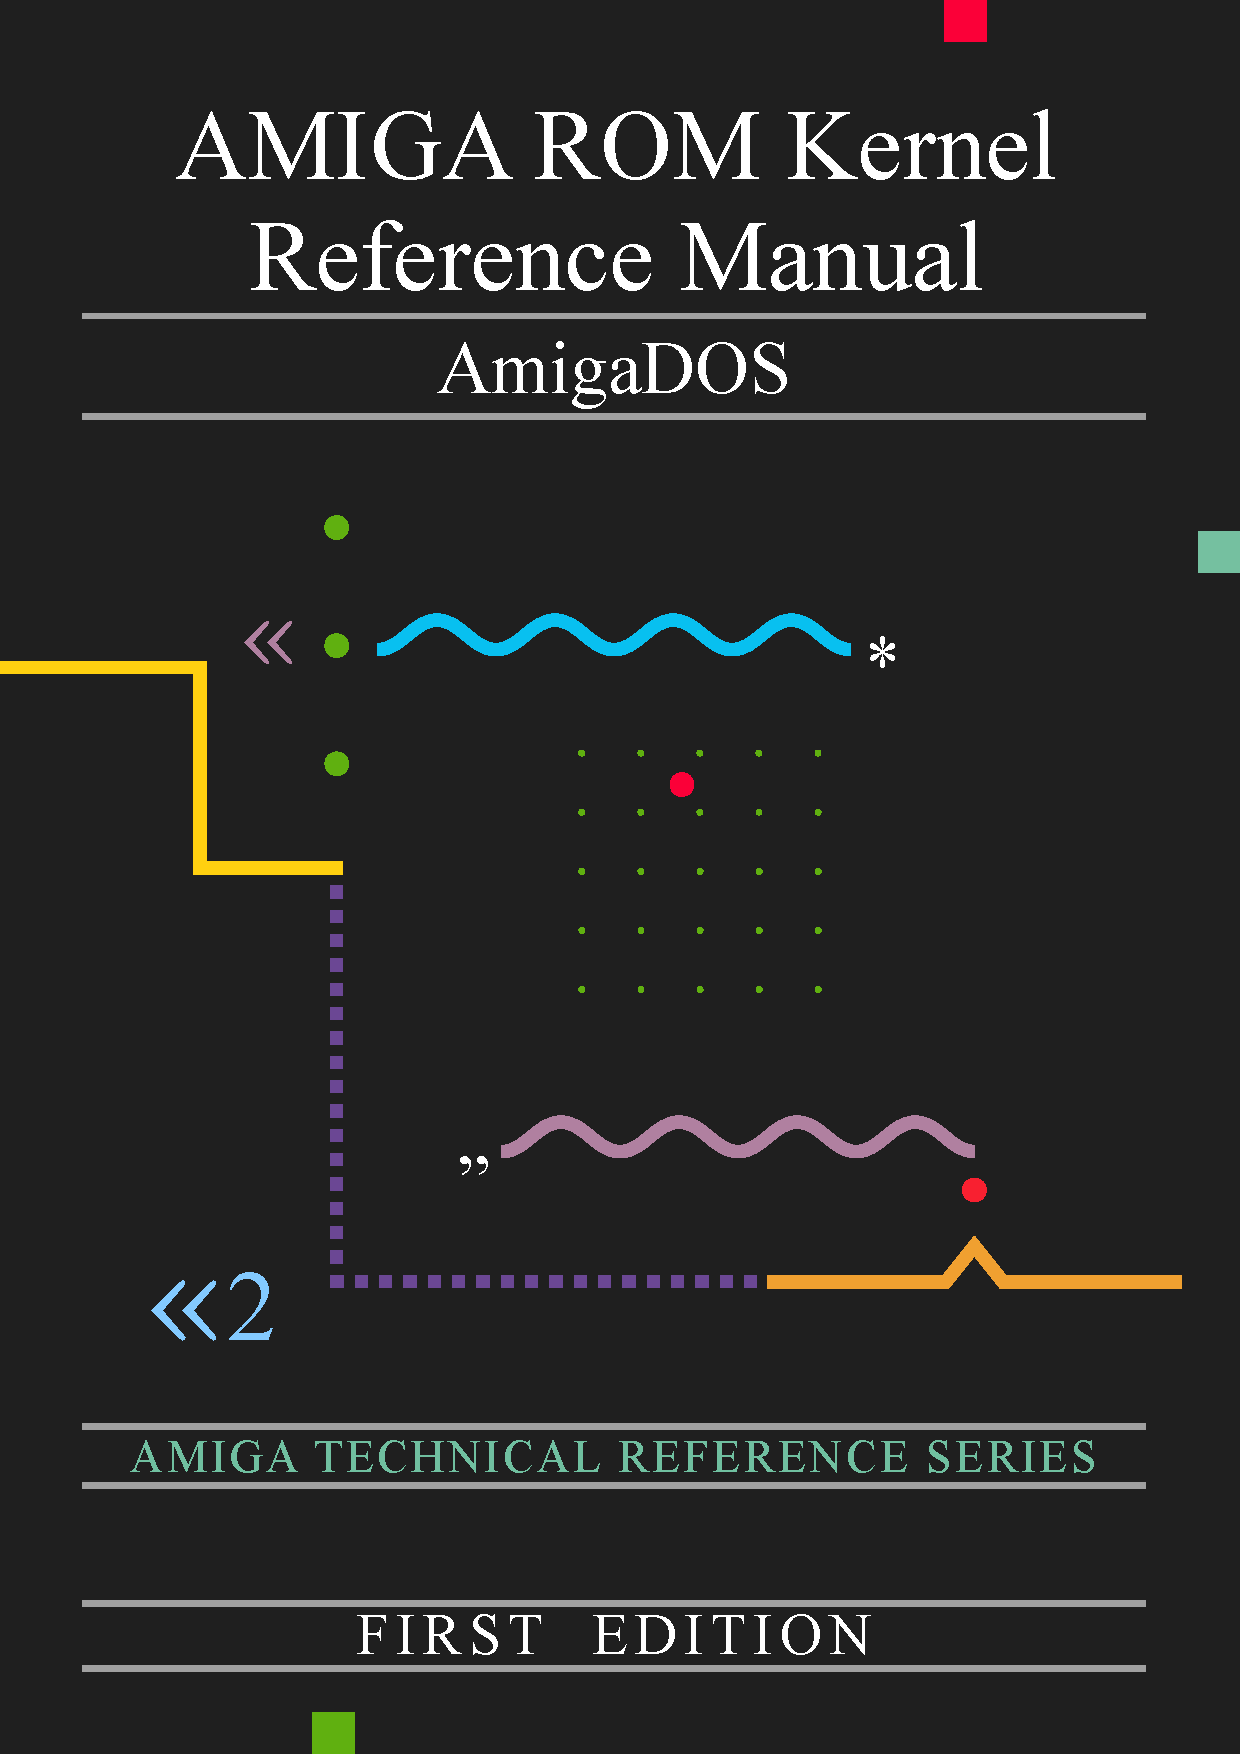
\includepdf[offset=-0.3cm -1cm]{front-page.pdf}
\newpage
\thispagestyle{empty}
\pagenumbering{roman}
\begin{center}
\vspace*{\fill}
{\Huge Amiga ROM Kernel Reference Manual\\}
\bigskip
{\Huge AmigaDOS\\}
\bigskip
{\huge\sc
Thomas Richter\\}
\bigskip
\end{center}
\bigskip
\vspace*{\fill}
\bigskip
{\small Copyright � 2024 by Thomas Richter, all rights reserved. This
publication is freely distributable under the restrictions stated below, but is
also Copyright � Thomas Richter.

Distribution of the Publication by a commercial organization without written
permission from the author to any third party is prohibited if any payment is
made in connection with such distribution, whether directly (as in payment for a
copy of the Publication) or indirectly (as in payment for some service related
to the Publication, or payment for some product or service that includes a
copy of the Publication ``without charge''; these are only examples, and
not an exhaustive enumeration of prohibited activities).

However, the following methods of distribution involving payment shall not in
and of themselves be a violation of this restriction:
\begin{enumerate}
\item Distributing the Publication on a physical data carrier (e.g.\ CD-ROM,
  DVD, USB-Stick, Disk...) provided that:
  \begin{enumerate}
  \item the Publication is reproduced entirely and verbatim on such data carrier,
    including especially this license agreement;
  \item the data carrier is made available to the public for a nominal
    fee only, i.e.\ for a fee that covers the costs of the data carrier,
    and shipment of the data carrier;
  \item a data carrier with the Publication installed is made available to the
    author for free except for shipment costs, and
  \item provided further that all information on said data carrier is
    redistributable for non-commercial purposes without charge.
  \end{enumerate}
\end{enumerate}

Redistribution of a modified version of the publication is prohibited in any
way, by any organization, regardless whether commercial or non-commercial.
Everything must be kept together, in original and unmodified form. }

\bigskip

{\small \sc Disclaimer: This publication is provided ``as is'' without any
warranty of any kind, either expressed or implied, including, but not limited
to, the implied warranties of merchantability and fitness for any particular
purpose. Further, the author does not warrant, guarantee, or make any
representation regarding the use of, or the results of the use of, the
information contained herein in term of correctness, accuracy, reliability,
currentness, or otherwise; the entire risk as to its quality and accuracy is
assumed solely by the user. Should the information prove inaccurate, the user
(and not the author) assumes the either cost of all necessary correction. In no
event will the author be liable for direct, indirect, incidental, or
consequential damages resulting from any defect or inaccuracy in this
publication, even if advised of the possibility of such damages. Some laws do
not allow the exclusion or limitation of implied warranties or liabilities for
incidental or consequential damages, so the above limitation or exclusion may
not apply.}

\bigskip

{\small {\it Amiga} is a registered trademark, {\it Amiga-DOS}, {\it Exec} and
{\it Kickstart} are registered trademarks of Amiga Intl. {\it Motorola} is a
registered trademark of Motorola, inc. {\it Unix} is a trademark of
the Open Group.}
\newpage
\vspace*{\fill}
\newpage
\tableofcontents
\pagenumbering{arabic}
%
%
\chapter{Introduction}
\section{Foreword}
The purpose of this manual is to provide a comprehensive documentation of
the AmigaDOS subsystem of the Amiga Operation System. AmigaDOS provides
elementary services similar to other contemporary operating systems, such as
file systems and handlers implementing stream-based input and output,
process management, volume and device management, command line execution and
command line parsing. Its interface to applications is the
\emph{dos.library}, a ROM based shared library that provides an interface
between such applications and AmigaDOS subsystems such as file systems or
the Shell.
\smallskip{}

While the Amiga ROM Kernel Reference Manuals~\cite{rkrmlib} document major
parts of the AmigaOs, they do not include a volume on AmigaDOS and its
subsystems. This is due to the history of AmigaDOS which is nothing but a
port of Tripos, an experimental operating system developed
at the University of Cambridge. Instead, its documentation became available
as the AmigaDOS manual~\cite{Bantam} separately. This book is, similar to
AmigaDOS, based on the Tripos manual which has been augmented and updated to
reflect the changes that were necessary to fit Tripos into
AmigaOs. Unfortunately, the book is now out of print, does not reflect the
current state of AmigaDOS anymore, and leaves multiple parts of AmigaDOS
undocumented.
\smallskip{}

Good third party documentation is available in the form of the Guru
Book~\cite{guru}, though this source is also out of print and even harder to
obtain. It also covers aspects of AmigaOs that go beyond AmigaDOS and its
focus is a bit different than that of this work.
\smallskip{}

This book attempts to fill this gap and attempts to provide a comprehensive
and complete documentation of AmigaDOS library and its subsystems, closely
following the style of the ROM Kernel Reference Manuals.

\subsection{Acknowledgments}

A book of this size would be impossible without additional help from
others. I want to thank in particular Frank Wille for helping me to compile
the description of the Amiga binary format and Olaf Barthel for many
fruitful discussions and for answering many questions while compiling many
chapters of this volume. Special thank goes to Rainer M{\"u}ller for
proof-reading the manuscript and providing many fixes and corrections.

\section{Language and Type Setting Conventions}
The words \emph{shall} and \emph{shall not} indicate normative
requirements software shall or shall not follow or in order to satisfy the
interface requirements of AmigaDOS. The words \emph{should} and
\emph{should not} indicate best practice and recommendations that are
advisable, but not strictly necessary to satisfy a particular
interface. The word \emph{may} provides a hint to a possible
implementation strategy.
\smallskip{}

The word \emph{must} indicates a logical consequence from existing
requirements or conditions that follows necessarily without
introducing a new restriction, such as in ``if $a$ is 2, $a+a$
\emph{must} be 4''.

\punchline{Worth remembering!}{Important aspects of the text are
  indicated with a bold vertical bar like this.}

Terms are indicated in \emph{italics}, e.g.\ the \emph{dos.library}
implements an interface of \emph{AmigaDOS}, and are also used when new terms are
introduced for the first time. Data structures and source code are printed
{\tt in courier} in fixed-width font, reassembling the output of a terminal,
e.g.\

\begin{verbatim}
typedef unsigned char UBYTE; /* an 8-bit unsigned integer */
typedef long LONG;           /* a 32-bit integer          */
\end{verbatim}

\chapter{Elementary Data Types}
\section{Purpose of the dos.library}
\emph{AmigaDOS} is part of the \emph{Amiga Operating System} or short
\emph{AmigaOs}. The \emph{dos.library} provides the application interface to
AmigaDOS, even though it consists of components beyond this library,
e.g.\ the \emph{AmigaDOS Shell} and the \emph{Fast File System}
\key{Fast File System (FFS)}, which is the default (ROM-based) file system organizing the
data on data carriers such as floppy disks or hard disks.
\smallskip{}

Unlike many other operating systems, the \emph{dos.library} does not manage
disks or files itself, neither does it provide access to hardware interface
components. It rather implements a \emph{virtual file system} which forwards
requests to its subsystems, called \emph{handlers}\mkey{Handler} or
\emph{file systems}\mkey{File System}. The FFS\key{Fast File System (FFS)} is only one of the multiple
file systems AmigaDOS is able to handle; instead, it provides an abstract
interface to handlers that allows its extension by third-party file systems
and handlers. Handlers and file systems are introduced in
section~\ref{sec:handlerovv}, and the interface between the
\emph{dos.library} and such handlers is specified in
chapter~\ref{sec:handlers}.

\section{The DosLibrary Object}

The \emph{dos.library} is typically opened by the startup code of most
compilers, and its base pointer is placed into the {\tt DOSBase}
object by such startup code:
\begin{verbatim}
struct DosLibrary *DOSBase;
\end{verbatim}
Hence, in general, there is no need to open this library manually.
\smallskip{}

The \emph{\mkey{DosLibrary}DosLibrary} structure is defined in
{\tt dos/dosextens.h}, but its elements are usually not required and should not
be accessed directly. However, chapter~\ref{sec:dosbase} provides further
details and provides information on its structure. The most important
function of the library is to provide functions to applications due to its
library vector offsets --- or short {\tt \_LVO}s --- which are made
available to a C compiler by including {\tt proto/dos.h}:

\begin{verbatim}
#include <proto/dos.h>
\end{verbatim}

This book is organized around groups of functions defined through the above
file, roughly by functionality and by increasing complexity.
\medskip{}

If you do not link with compiler startup code, the base pointer of the
\emph{dos.library} is obtained similar to any other AmigaOs library:
\begin{verbatim}
#include <proto/exec.h>
#include <proto/dos.h>
#include <exec/libraries.h>
#include <dos/dos.h>

struct DosLibrary *DOSBase;
struct ExecBase *SysBase;

int __saveds startup(void)
{
  SysBase = *((struct ExecBase **)(4L);
  ...
  if ((DOSBase = (struct DosLibrary *)(OpenLibrary(DOSNAME,47)))) {
    ...
    CloseLibrary((struct Library *)DOSBase);
  }
  ...
}
\end{verbatim}
The most up to date version of the \emph{dos.library} also discussed in this
book is~$47$, as indicated by the second argument of
{\tt OpenLibrary()}. Not all
programs will require its most recent version,
though; the version in which a particular function of the \emph{dos.library}
appeared is indicated behind the function definition. Rather
than requesting the maximum version, program authors should identify which
functions of the library they require, identify for each of them the minimum
version number in which they became available, and then take the maximum of
all the version numbers and supply this maximum as second argument of
{\tt OpenLibrary()}. Table~\ref{table:dosversions} provides the relation
between AmigaDOS versions and the corresponding library
version:

\begin{rkrmtable}{AmigaDOS Version Numbers} \label{table:dosversions}
{\bf AmigaDOS version} & {\bf dos.library version}\\ \hline \hline
1.2 & 33 \\ \hline
1.3 & 34 \\ \hline
1.4 {\small (RAM-based, with Hedley support)} & 35 \\ \hline
2.0 & 36 \\ \hline
2.04 & 37 \\ \hline
2.1 & 38 \\ \hline
3.0 & 39 \\ \hline
3.1 & 40 \\ \hline
3.1 {\small (unpublished, with support for Japanese locale)} & 41 \\ \hline
3.1 {\small (unpublished alpha release)} & 42 \\ \hline
3.2 {\small (unpublished release for the Walker)} & 43 \\ \hline
3.5 & 44 \\ \hline
3.9 & 45 \\ \hline
3.1.4 & 46 \\ \hline
3.2 & 47 \\ \hline
\end{rkrmtable}

Version 35 was an extension of version 34 with
integrated support for the A2024 Hedley monitor that was entirely
RAM-loaded. Most important changes were made in version 36 in which the library was
largely extended, though the release contained many defects that were
addressed in version 37. Version 38 was a pure software update that added
localization support. Versions 41 to 43 were never published, with the exception of
some beta versions of the FFS which shipped as version 43. Version 44 was used for
AmigaOs 3.5, and 45 for AmigaOs 3.9 and most modules of 3.1.4. Some modules
with extended features such as the FFS\key{Fast File System (FFS)} with long
file name support received the version number 46.

\section{Booleans}

AmigaDOS uses a convention for Booleans that differs from the one
imposed by the C programming language; it uses the following truth
values defined in the file {\tt dos/dos.h}:

\begin{rkrmtable}{DOS Truth Values} \label{table:dosbool}
{\bf Define} & {\bf Value}\\ \hline \hline
DOSFALSE & \phantom{-}0  \\ \hline
DOSTRUE  & -1 \\ \hline
\end{rkrmtable}

Note that the C language instead uses the value~$1$ for
{\tt TRUE}. Code that checks for zero or non-zero return codes will
function normally, however code shall not compare to {\tt TRUE} in
Boolean tests. Instead, tests shall be made whether particular values are~0
or different from~0, avoiding this discrepancy between the conventions of
AmigaDOS and the C language.

\section{Pointers and BPTRs} \label{sec:bptrs}
AmigaDOS is a descendant of the \emph{Tripos} operating system and as such
was originally implemented in the BCPL language. As of Kickstart 2.0,
i.e.\ version 36 of the \emph{dos.library}, AmigaDOS was re-implemented in C
and assembler, but this implementation had to preserve the existing
interface based on BCPL conventions.
\smallskip{}

BCPL is a type-less language that structures the memory of its host system as
an array of 32-bit elements enumerated contiguously from zero up. Rather
than pointers, BCPL communicates the position of its data structures in the
form of the index of the first 32-bit element of a structure in memory. As
each 32-bit group is assigned its own index, one can obtain this index by
dividing the byte-address of an element by 4, or equivalently, by
right-shifting the address as given by a pointer of the C language by two
bits. This also has the consequence that (most) data structures passed into
and out of the \emph{dos.library} shall be aligned to 32-bit boundaries. Similarly,
in order to obtain the byte-address of a BCPL structure, its index is
multiplied by 4, or left-shifted by 2 bits.

\punchline{Not on the Stack!}{Since BCPL structures must have an address
  that is divisible by 4, using automatic storage duration for AmigaDOS
  objects is inappropriate. Compilers will typically keep such objects on
  the hardware stack of the 68K processor~\cite{mcfam,yuchen}, but usually do not
  ensure that their addresses are aligned to long word boundaries. In case a
  particular AmigaDOS object cannot be constructed by
  \key{AllocDosObject()}{\tt AllocDosObject()} (see
  section~\ref{sec:allocdosobject}), a safe strategy is use \emph{exec.library}
  memory allocation functions such as {\tt AllocMem()} or
  {\tt AllocVec()} to obtain memory for holding them. All
  three functions ensure proper alignment.}

Indices to 32-bit memory cells in the BCPL abstraction of computer memory
are called \emph{BCPL pointers} or short \emph{\key{BPTR}BPTR}s, even though
they are not pointers in the sense of the C language; they are rather
integer numbers as indices to an array of {\tt LONG} (i.e.\ 32-bit)
integers. In order to communicate this fact more clearly, the
{\tt dos/dos.h} include file defines the following data type:

\mkey{BPTR}
\begin{verbatim}
typedef long  BPTR;                 /* Long word pointer */
\end{verbatim}

The include file {\tt exec/types.h} contains the definition of an untyped C
pointer as follows:
\mkey{APTR}
\begin{verbatim}
typedef void *APTR;                 /* 32-bit untyped pointer */
\end{verbatim}
This is, unlike a BPTR a real pointer, though the data type it points to
remains undefined.
\smallskip{}

Conversion from BCPL pointers to conventional C pointers and back are
realized by the following macros, also defined in {\tt dos/dos.h}:

\mkey{BADDR()} \mkey{MKBADDR()}
\begin{verbatim} 
/* Convert BPTR to typical C pointer */
#define BADDR(x)        ((APTR)((ULONG)(x) << 2))
/* Convert address into a BPTR */
#define MKBADDR(x)      (((LONG)(x)) >> 2)
\end{verbatim}

Luckily, in most cases callers of the \emph{dos.library} do not need to
convert from and to BPTRs but can rather use such ``pointers'' as
\emph{opaque values} or \emph{handles} representing some AmigaDOS
object. Examples for those objects are \emph{file handles}\key{FileHandle} specified in
chapter~\ref{sec:file}, and \emph{locks}\key{Lock}, see chapter~\ref{sec:locks}. Both
are represented as BPTRs to some structure the caller usually does not need
to care about.
\smallskip{}

It is certainly a burden to always allocate temporary BCPL objects from the
heap through the \emph{exec.library} or the \emph{dos.library}, and doing so
can also fragment the AmigaOs memory unnecessarily. However, allocation of
automatic objects from the stack does not ensure long-word alignment in
general. To work around this burden, one can use a trick and instead request
from the compiler a somewhat longer object with automatic storage duration
and align the requested object manually within the memory obtained this
way. The following macro performs this trick:

\mkey{D\_S() macro}
\begin{verbatim}
#define D_S(type,name) char a_##name[sizeof(type)+3]; \
                       type *name = (type *)((ULONG)(a_##name+3) & ~3UL)
\end{verbatim}

It is used as follows:
\begin{verbatim}
D_S (struct FileInfoBlock, fib); 
\end{verbatim}

At this point, fib is a pointer to a properly aligned {\tt struct
FileInfoBlock}, e.g.\ this is equivalent to
\begin{verbatim}
struct FileInfoBlock _tmp;
struct FileInfoBlock *fib = &tmp;
\end{verbatim}
except that the created pointer is properly aligned and can safely be
passed into the \emph{dos.library}.
\smallskip{}

Similar to the C language, a pointer to a non-existing element is
expressed by the special pointer value~$0$. While this is called the
{\tt NULL} pointer in C, it is better to reserve another name for it
in BCPL as BPTRs are indices instead. The following convention
is suggested to express an invalid BPTR:

\begin{verbatim}
#define ZERO 0L
\end{verbatim}

Clearly, with the above convention, the BCPL {\tt \mkey{ZERO}ZERO} pointer
converts to the C {\tt \mkey{NULL}NULL} pointer and back, even though the two are
conceptually something different: The first being the index to the
first element of the host memory array, the later the pointer to the
first address.

\section{C Strings and BSTRs}
While the C language defines \emph{\mkey{String (C)}strings} as
0-terminated arrays of {\tt char}, and AmigaOs in particular to
0-terminated arrays of {\tt UBYTE}s, that is, unsigned characters, the
BCPL language uses a different convention. Instead, a BCPL
string\mkey{String (BCPL)} is a {\tt UBYTE} array whose first element
contains the size of the string to follow. They are not necessarily
0-terminated either. If BCPL strings
are passed into BCPL functions, or are part of BCPL data structures,
then typically in the form of a BPTR\key{BPTR} to the 32-bit
element containing the size of the string its 8 most significant
bits. The include file {\tt dos/dos.h} provides its own data type for
such strings:

\mkey{BSTR}
\begin{verbatim}
typedef long  BSTR;   /* Long word pointer to BCPL string  */
\end{verbatim}

Luckily, functions of the \emph{dos.library} take C strings as
arguments and perform the conversion from C strings to their BCPL
representation as \emph{BSTR}s internally, such that one rarely gets
in contact with this type of strings. They appear as part of some
AmigaDOS structures to be discussed, and as part of the interface
between the \emph{dos.library} and its handlers, e.g.\ file systems.
However, even though users of the \emph{dos.library} rarely come in
contact with BSTRs themselves, the BCPL convention has
an important consequence, namely that (most) strings handled by the
\emph{dos.library} cannot be longer than 255 characters as this is the
maximum value an byte-sized length value can take.

\punchline{Length-Limited Strings}{Remember that most strings that are
  passed into the \emph{dos.library} are internally converted to
  BSTRs and thus cannot exceed a length of 255 characters.}

Unfortunately, even in the latest version of \emph{AmigaDOS}, the
\emph{dos.library} is ill-prepared to take longer strings, and will
likely fail or mis-interpret if such strings are passed in. If longer strings
are required, e.g.\ as part of a \emph{path}, it is
(unfortunately) in the responsibility of the caller to take this path
apart into components and iterate through the components manually,
see also section~\ref{sec:paths}.
\smallskip{}

Finally, the {\tt NUL} character --- note the single ``{\tt L}'' --- is the
name of the ASCII character with code~0 by which all C strings are
terminated. A C string is therefore a {\tt NUL}-terminated string. This
notation will be used throughout this volume.

\punchline{All Zero, but of a Different Kind}{{\tt ZERO},
{\tt NULL} and {\tt NUL} all encode the value 0, but the first is the name
of the first BCPL memory index and indicates an invalid BPTR.
Its C equivalent is {\tt NULL}, which however denotes a pointer
and not a memory cell index. {\tt NUL} is the first code
point of the ASCII code set and represented by a byte of value~0.}

\section{Elementary Conversion Functions}

Functions in this section perform conversions between the elementary data
types listed in this chapter, and convert between strings representing numbers as
human-readable decimals and their binary machine representations. The
{\tt StrToLong()}\key{StrToLong()} takes such a string and converts it to an
integer. There is no function in the \emph{dos.library} to perform the
inverse conversion of an integer into a string, though the \emph{exec.library}
function {\tt RawDoFmt()}\key{RawDoFmt()} may be used to implement it as a by-product of a
more general family of functions. Section~\ref{sec:printf} provides a very
compact and in many cases sufficient implementation of a function that
closely reassembles the {\tt sprintf()}\key{sprintf()} function of ANSI-C;
it prints and formats many elementary data types, including integers, into an output
buffer, and as such, can also convert an integer into a decimal number.

\subsection{Convert a String to a Number} \label{sec:strtolong}

The {\tt StrToLong()}\mkey{StrToLong()} function converts an ASCII encoded
decimal number to a signed 32 bit integer.

\begin{verbatim}
characters = StrToLong(string,value) /* since V36 */
D0                      D1    D2

LONG StrToLong(STRPTR, LONG *)
\end{verbatim}

This function converts the {\tt NUL}-terminated {\tt string} containing a
decimal number encoded in ASCII and converts it to a signed integer. The
return value is the number of characters it could interpret from the string,
or $-1$ if not a single valid digit could be found. The converted number is
placed into the 32-bit long word pointed to by {\tt value}.
\smallskip{}

The function skips leading spaces and tabs, they are included in
{\tt characters}. It also interprets a leading minus sign
(``{\tt -}'') to indicate negative numbers, but \emph{does not} accept a
leading plus sign (``{\tt +}''). This function also aborts in case the
conversion overflows, i.e.\ the absolute value of the number is larger than
$2^{31}$, and then returns the number of characters up to which the
conversion could be performed without overflow. The output of the conversion
filled into {\tt value} is in this case meaningless.
\smallskip{}

Even in case of error, this function does not alter {\tt IoErr()}\key{IoErr()}.

\subsection{Print Formatted into a Buffer} \label{sec:sprintf}

While not a function of the \emph{dos.library}, the code segment in this
section implements a function similar to the {\tt sprintf()} function of the
ANSI C library; it converts many elementary data types to
strings. It is based on the {\tt RawDoFmt()}\mkey{RawDoFmt()} function of the
\emph{exec.library}, which is also patched by the \emph{locale.library} and
thus converts numbers according to the currently loaded locale.

\mkey{sprintf()}\mkey{vsprintf()}\mkey{LongToStr()}
\begin{verbatim}
#include <stdarg.h> /* for va_list macros */

static void prbuf(char c)
{
  __builtin_emit(0x16c0);   /* move.b D0,(A3)+ */
}

/*
** convert a list of arguments to a string using an
** ANSI-C format template.
*/
void vsprintf(char *buffer, const char *ctlstr, void *args)
{
  RawDoFmt((char *)ctlstr, args, prbuf, buffer);
}

/*
** Convert multiple arguments to a string, using
** an ANSI-C format template.
*/
void sprintf(char *buffer, const char *ctrl,...)
{
  va_list args;

  va_start(args,ctrl);
  vsprintf(buffer,ctrl,args);
  va_end(args);
}

/*
** Convert a signed integer to a string
*/
void LongToStr(char buffer *buf, LONG val)
{
  sprintf(buffer,"%ld",val);
}
\end{verbatim}
The {\tt vsprintf()} function defined above takes a target {\tt buffer}, an ANSI-C
conversion string {\tt ctlstr} containing formatting directives, see~\cite{kernrichie},
and a buffer of primitive integer data types or strings in {\tt args}. It
converts these arguments to strings, formats them according to {\tt ctlstr}
and places the result in the target buffer. The full set of conversion
directives is found in the description of
{\tt RawDoFmt()}\key{RawDoFmt()} in~\cite{rkrmlib}, though the most elementary directives
are shown here:

\begin{itemize}
\item[\tt \%s] The next argument in {\tt args} is a pointer to a
  {\tt NUL}-terminated string that is inserted into {\tt buffer}. To limit
  the number of characters copied into the target buffer, an ANSI-C
  precision field should
  be included in the format directive, e.g.\ {\tt \%.30s} truncates the
  input string to 30 characters.
\item[\tt \%b] The next argument is a BPTR to a BSTR that is inserted into the
  {\tt buffer}. This formatting directive was added in AmigaOs version~36. Again,
  it is recommended to truncate the string length by the ANSI-C precision
  format directive, see above.
\item[\tt \%ld] The next argument in {\tt args} is a 32-bit signed integer
  that is converted to a decimal string.
\item[\tt \%lu] Convert a 32-bit unsigned integer to a decimal string --- this formatting directive was added in
  AmigaOs~37.
\item[\tt \%lx] Convert a 32-bit unsigned integer to hexadecimal. If needed,
  a leading {\tt 0x} must be inserted manually, it is not part of the output
  of the conversion.
\item[\tt \%lc] Interpret a 32-bit integer as an ISO-Latin or ASCII code
  point and insert a single character this code point represents.
\end{itemize}

As also seen above, the ANSI-C flags, field width, precision and length
modifiers may be included in the format directive starting
with ``{\tt \%}'', see~\cite{rkrmlib} for more details. 

\punchline{Think Long}{The knowledgeable C developer will notice that many
  of the above conversion directives include an {\tt l} length modifier
  which has been added here on purpose, even causing strange directives such
  as {\tt \%lc}. This is because the {\tt RawDoFmt()} function assumes a
  16-bit integer model, whereas most compilers operate with 32-bit
  integers. The length modifier ensures that the \emph{exec.library} removes
  32-bit arguments from {\tt args}, corresponding to the integer
  size of many C implementations. Some older compilers use, in fact, a 16-bit
  integer model in which case the {\tt l} shall be dropped (but only
  then!). Not following this guideline will cause hard to find bugs
  resulting in incorrect output.}

The {\tt vsprintf()}\key{vsprintf()} function from the above code segment implements the function
of the same name in the ANSI-C library only approximately, and the
formatting directives need to be adjusted carefully to avoid problems. There
is, as in the ANSI-C standard library, no check whether the target buffer is
large enough. In particular, string formatting directives should be selected
carefully to avoid buffer overruns that can lead to system crashes. As the
{\tt FPrintf()}\key{FPrintf()} function from section~\ref{sec:fprintf} and
the {\tt Printf()}\key{Printf()} function from section~\ref{sec:printf} are
based on the same exec function, the same peculiarities apply there as well.
\smallskip{}

The {\tt sprintf()}\key{sprintf()} function is an --- albeit basic ---
re-implementation of the C standard library function {\tt sprintf()} which
prints all its arguments to a buffer. The same formatting directives apply.
It uses the varargs macros of ANSI-C from {\tt stdarg.h} to forward its
arguments to {\tt vsprintf()}.
\smallskip{}

The {\tt LongToStr()}\key{LongToStr()} function is a simple application
of {\tt sprintf()} to convert a signed integer to a string. It does the inverse of the
{\tt StrToLong()}\key{StrToLong()} function of the \emph{dos.library}
introduced in section~\ref{sec:strtolong}.
\smallskip{}

The {\tt prbuf()} function is hack using a built-in function of the SAS/C
compiler. Its function body consists only of the {\tt \_\_builtin\_emit()}
function which injects the object code of the {\tt MOVE.B D0,(A3)+}
instruction into the function body. It takes
the function argument placed in register {\tt D0}
by {\tt RawDoFmt()}\key{RawDoFmt()} and pushes it into the target buffer pointed to by
register {\tt A3}. Other compilers will need a small assembler stub function
of the same name that consists only of this instruction, and an {\tt RTS}.

\section{Files}
Files\key{File} are streams of bytes together with a file pointer that
identifies the next position to be read, or the next byte position to write
to. Files are explained in more detail in chapter~\ref{sec:file}. AmigaDOS
represents files through \emph{file handles}\key{FileHandle} in the form of
a BPTR to a \emph{FileHandle}\mkey{FileHandle} structure, though most of the
time, the elements of the structure are not needed and it is sufficient to
pass the BPTRs around.

\section{Locks}
Locks\key{Lock} are access rights to a particular object on a file system,
such as a file or a directory. A locked file cannot be overwritten or removed by
any other process, a locked directory can be altered, but not be
deleted. Chapter~\ref{sec:locks} provides more details on locks. AmigaDOS
represents locks through the \emph{FileLock}\key{FileLock} structure also
introduced in the above chapter, though in most cases, locks\key{Lock} are passed
around as BPTRs to this structure.

\section{Processes}
AmigaDOS is a multi-tasking system operating on top of the \emph{exec}
kernel~\cite{rkrmlib}. As such, it can operate multiple tasks at once, where
the tasks are assigned to the CPU in a round-robin fashion. A
\emph{Process}\key{Process} is an extension of an AmigaOs
\emph{Task}\mkey{Task}; it includes additional state information relevant
to AmigaDOS, such as a \emph{current directory}, a default file
system, a \emph{console}\key{Console} it is connected to, and default input,
output and error streams. Most important, each process includes a {\tt
  MsgPort}, see~\cite{rkrmlib}, through which it communicates with other
AmigaDOS components such as handlers or file systems. Processes are
explained in more detail in chapter~\ref{sec:process}.

\section{Handlers and File Systems} \label{sec:handlerovv}
\emph{Handlers} are special processes that perform input or output
operations to logical or physical devices, such as the serial port, a
printer, the floppy or even the RAM. The \emph{dos.library} delegates most
operations, such as reading from a stream or file to such handlers. Handlers
are explained in more detail in chapter~\ref{sec:handlers}.
\smallskip{}

\emph{File systems} are special handlers that organize the contents of data
carriers such as hard disks, floppies or CD-Roms in the form of files and
(optionally) directories. File systems interpret paths (see~\ref{sec:paths})
in order to locate objects such as files and directories on data
carriers. Thus, every file system is a handler --- i.e.\ the Fast File System
(FFS) is a handler, discussed in section~\ref{sec:ffs} --- but not every
handler implements a file system. The console window, for example, is
provided by the CON-Handler\key{CON-Handler} in the form of the
{\tt CON} device, even though it surely does not organize
files. Section~\ref{sec:console} provides more details on this
particular handler.

\section{The AmigaDOS Shell}

The AmigaDOS Shell is a command line interpreter and implements a (basic)
programming language through which the user can communicate with the
system. Historically, the Shell was also called the \emph{CLI} for
\emph{Command Line Interface}, and it is the primary user interface of
AmigaDOS. Unlike the graphical user interface, the Workbench, it is purely
text based and available even without a boot medium.
\smallskip{}

The Shell reads lines from the console, which is a handler of its own, and
interprets them as commands, potentially along with additional
arguments to them. Commands are binary executable files (see
chapter~\ref{sec:binary} for their structure) that are contained in a
special directory of an AmigaDOS installation, though some elementary
commands are built into the Shell and do not require access to a medium.
\smallskip{}

The Shell is not restricted to reading commands from the console. Any other
handler can serve as source as well, for example in the form of a
\emph{Shell Script} or \emph{Batch File} located on a partition operated by
the Fast File System (FFS)\key{Fast File System (FFS)}, the Amiga ROM file
system. The most important Shell script\key{Shell Script} is the
\emph{Startup-Sequence}\key{Startup-Sequence} which is interpreted by the Shell when booting
AmigaOs. Chapter~\ref{sec:shell} provides more details on the AmigaDOS Shell.
\smallskip{}

AmigaDOS is not limited to its own Shell\key{Shell}, which is also called the Boot
Shell\key{Boot Shell}; even though this feature is rarely used, users may install additional
alternative shells. The AmigaDO
S interface to shells is specified in
section~\ref{sec:usershells}.

\chapter{Date and Time} \label{sec:dates}

Due to its history, AmigaOs uses two incompatible representations of date
and time. The {\tt timer.device} represents a date as the number of seconds
and microseconds since January $1^{\mbox{\tiny st}}$ 1978. As AmigaDOS is
based on Tripos as an independently developed operating system, the
\emph{dos.library} uses a different representation as {\tt DateStamp}
structure defined in {\tt dos/dos.h}: \mkey{DateStamp (struct)}
\begin{verbatim}
struct DateStamp {
   LONG  ds_Days;
   LONG  ds_Minute;
   LONG  ds_Tick;
};
\end{verbatim}

The elements of this structure are as follows:
\smallskip{}

{\tt ds\_Days}\mkey{ds\_Days} counts the number of days since January
$1^{\mbox{{\tiny st}}}$ 1978. It includes intercalary days added
approximately all four years at the end of February.
\smallskip{}

{\tt ds\_Minute}\mkey{ds\_Minute} counts the number of minutes past midnight, i.e.\ the start of the day.
\smallskip{}

{\tt ds\_Tick}\mkey{ds\_Tick} counts the ticks since the start of the minute. The number of
ticks per second is defined as {\tt TICKS\_PER\_SECOND} in {\tt
  dos/dos.h}. The ticks, and the seconds that can be derived from it, do not
include leap seconds that are added from time to time. In case leap seconds
are added, the Amiga clock needs to be adjusted manually.
\smallskip{}

\punchline{Ticking 50 Times a Second}{A system ``tick'' is always
$1/50^{\mbox{\tiny th}}$ of a second, regardless whether the system is an
NTSC or PAL system. AmigaDOS detects the clock basis during setup and will
scale times appropriately such that the definition of the ``tick'' is
independent of the clocking of the system or the monitor refresh frequency.}

The system date, or rather the functions to convert between the Amiga
{\tt timer.device} representation and the AmigaDOS {\tt DateStamp}\key{DateStamp (struct)}
representation is currently limited to $31^{\mbox{\tiny th}}$ December
2045. There is no function in AmigaDOS to set the date, this needs to be
done through the {\tt timer.device} with the {\tt TR\_SETSYSTIME}
command. The Kickstart, during bootstrap, takes the current time from the
real time clock, if it is present. If no real time clock is present, then
all elements of the {\tt rn\_Time} structure in the {\tt RootNode} structure
(see section~\ref{sec:rootnode}) of the \emph{dos.library} remain~0,
corresponding to a system date of January $1^{\mbox{\tiny st}}$ 1978. The
boot file system shall check this condition and provide a better
approximation in such a case. The FFS\key{Fast File System (FFS)} will use in this case the creation
time of the boot volume recorded in the root block, see
section~\ref{sec:rootblock} and adjusts the system time then through the
{\tt timer.device}.

\section{Elementary Time and Date Functions}

The functions in this section obtain the current system time, compare two
times, or delay the system for a given time. They represent times --- and
dates if appropriate --- in the {\tt DateStamp}\key{DateStamp (struct)} structure as a triple of
days, minutes and ticks.

\subsection{Obtaining the Time and Date} \label{sec:datestamp}

The {\tt DateStamp()}\mkey{DateStamp()} function obtains the current date
and time from AmigaDOS:

\begin{verbatim}
ds = DateStamp( ds );
D0              D1

struct DateStamp *DateStamp(struct DateStamp *)
\end{verbatim}

This function retrieves the current system time and fills it into a
{\tt DateStamp}\key{DateStamp (struct)} structure pointed to by {\tt ds}. It also
returns a pointer to the structure passed in. This function cannot fail.
\smallskip{}

Unlike many other \emph{dos.library} functions, there is no requirement to
align {\tt ds} to a long-word boundary.

\subsection{Comparing two Times and Dates}

The {\tt CompareDates()}\mkey{CompareDates()} function compares two dates as
given by {\tt DateStamp}\key{DateStamp (struct)} structures and returns an indicator
which of the dates are earlier.

\begin{verbatim}
result = CompareDates(date1,date2) /* since V36 */
D0                     D1     D2

LONG CompareDates(struct DateStamp *,struct DateStamp *)
\end{verbatim}

This function takes two pointers to {\tt DateStamp} structures as
{\tt date1} and {\tt date2} and returns a negative number if {\tt date1} is later
than {\tt date2}, a positive number if {\tt date2} is later than {\tt date1},
or~0 if the two dates are identical.
\smallskip{}

This function does not check the dates for validity, and it also assumes
that difference between the days does not exceed $2^{31}$ days. Note that
the logic of this function is different from {\tt strcmp()} and related
functions of ANSI-C, which return a positive number if its first argument is
larger than its second.

\subsection{Delaying Program Execution} \label{sec:delay}

The {\tt Delay()}\mkey{Delay()} function delays the execution of the calling
process by a specific amount of ticks.

\begin{verbatim}
Delay( ticks )
       D1

void Delay(ULONG)
\end{verbatim}

This function suspends execution of the calling process by {\tt ticks}
AmigaDOS ticks. The delay is system-friendly and does not burn CPU cycles;
instead, the process is suspended from the CPU the indicated amount of time,
making it available to other processes. Thus, this function is the
preferred way of delaying program execution. A tick is
$1/50^{\mbox{\tiny th}}$ of a second.
\smallskip{}

AmigaDOS variants below version 36 could not handle delays of~0 ticks
appropriately, thus passing a~0 argument should be avoided.

\section{Conversion Into and From Strings} \label{sec:dateconv}

Functions in this section convert date and time in the (binary) AmigaDOS
representation to human-readable strings, and in the reverse direction.
Both the input and output of these functions are kept in the
{\tt DateTime} structure that is defined in {\tt dos/datetime.h}
and reads as follows:
\mkey{DateTime}
\begin{verbatim}
struct DateTime {
        struct DateStamp dat_Stamp;
        UBYTE   dat_Format;        
        UBYTE   dat_Flags;         
        UBYTE   *dat_StrDay;       
        UBYTE   *dat_StrDate;      
        UBYTE   *dat_StrTime;      
};
\end{verbatim}

{\tt dat\_Stamp}\mkey{dat\_Stamp} contains the input or output date
represented as a {\tt DateStamp}\key{DateStamp (struct)} structure.
\smallskip{}

{\tt dat\_Format}\mkey{dat\_Format} defines the format of the date string to create, and the
order in which days, months and years appear within the string. The
following formats are available, all defined in {\tt dos/datetime.h}:

\begin{rkrmtable}{Date Formatting Options} \label{table:dateformats}
{\bf Format Definition} & {\bf Description} \\ \hline \hline
{\tt FORMAT\_DOS} & The AmigaDOS default format \\ \hline
{\tt FORMAT\_INT} & International (ISO) format \\ \hline
{\tt FORMAT\_USA} & USA date format \\ \hline
{\tt FORMAT\_CDN} & Canadian and European format \\ \hline
{\tt FORMAT\_DEF} & The format defined by the locale \\ \hline
\end{rkrmtable}

{\tt FORMAT\_DOS}\mkey{FORMAT\_DOS} represents the date as day of the month in two digits,
followed by the month as three-letter abbreviation, followed by a two-digit
year counting from the start of the century. An example of this formatting
is {\tt 30-Sep-23}.
\smallskip{}

{\tt FORMAT\_INT}\mkey{FORMAT\_INT} starts with a two-digit year, followed by the month
represented as two digits starting from 01 for January, followed by two
digits for the day of the month. An example of such a date is
{\tt 23-09-30}.
\smallskip{}

{\tt FORMAT\_USA}\mkey{FORMAT\_USA} places the month first, encoded as two numerical digits,
followed by two digits of the day of the month, followed by two digits of
the year. An example of this formatting is {\tt 09-30-23}.
\smallskip{}

{\tt FORMAT\_CDN}\mkey{FORMAT\_CDN} follows the European convention and places the day of the
month first, followed by the month represented as two numerical digits,
followed by the year as two digits.
\smallskip{}

{\tt FORMAT\_DEF}\mkey{FORMAT\_DEF} uses the format defined by the locale
settings of the system if the \emph{locale.library} is installed. Otherwise,
it falls back to {\tt FORMAT\_DOS}.
\smallskip{}

Unfortunately, it seems that the current NDK does not seem to define this
format, yet it is properly handled. Its definition should therefore be
performed manually as such:
\begin{verbatim}
#ifndef FORMAT_DEF
# define FORMAT_DEF 4
#endif
\end{verbatim}
\medskip{}

{\tt dat\_Flags}\mkey{dat\_Flags} defines additional flags that control the conversion
process. They are also defined in {\tt dos/datetime.h}:

\begin{rkrmtable}{Date Conversion Flags} \label{table:dateflags}
{\bf Flag} & {\bf Description} \\ \hline \hline
{\tt DTF\_SUBST} & Substitute dates by relative description if possible \\ \hline
{\tt DTF\_FUTURE} & Reference direction for relative dates is to the future\\ \hline
\end{rkrmtable}

The include file {\tt dos/datetime.h} define in addition also bit numbers
for the above flags that start with {\tt DTB} instead of {\tt DTF}. The
meaning of these flags are as follows:
\smallskip{}

{\tt DTF\_SUBST}\mkey{DTF\_SUBST} allows, if set, the conversion to
substitute dates nearby today's date by descriptions relative to today. This
flag is only honored when converting a time and date in AmigaDOS
representation to human-readable strings, and is for example used by the
{\tt List} command. In particular, the following substitutions are made:
\smallskip{}

If the date provided is identical to the system date, the output date is set
to ``{\tt Today}'', or a corresponding localized string if the
\emph{locale.library} is loaded.
\smallskip{}

If the date is one day later than the current system date, the output date
is set to ``{\tt Tomorrow}'', or to an appropriate localized version of this string.
\smallskip{}

If the date is one day before the current system date, the output date is set
to ``{\tt Yesterday}'', or a localized version of this string.
\smallskip{}

If the date is in the past week, the function substitutes it by the name of the
day of the week, e.g.\ ``{\tt Saturday}'', or its localized version.
\smallskip{}

A date in the future is substituted by ``{\tt Future}'', or its localized version.
\medskip{}

{\tt DTF\_FUTURE}\mkey{DTF\_FUTURE} is only only honored when converting a string to the
AmigaDOS representation, that is into {\tt DateStamp} structure. It
indicates whether weekdays such as ``{\tt Monday}'' are interpreted as dates in
the past, i.e.\ ``last Monday'', or as dates in the future, i.e.\ ``next
Monday''. If the flag is cleared, weekdays are interpreted as being in the
past, same as the {\tt DateToStr()}\key{DateToStr()} function would generate
them. If the flag is set, weekdays are assumed as references to the
future.
\medskip{}

{\tt dat\_StrDay}\mkey{dat\_StrDay}: This buffer is only used when converting {\tt DateStamps}
to strings, and --- if present --- is then filled by the week of the day,
e.g.\ ``{\tt Saturday}''. This buffer, as well as all other output buffers, needs to be at least
{\tt LEN\_DATSTRING} bytes long.
\smallskip{}

{\tt dat\_StrDate}\mkey{dat\_StrDate}: This element points to a buffer that is either filled
with the human-readable date, or is input to the conversion then containing
a human-readable date. The buffer is formatted, or expected to be formatted
according to {\tt dat\_Format} and {\tt dat\_Flags}.
\smallskip{}

{\tt dat\_StrTime}\mkey{dat\_StrTime}: This element points to a buffer that is either filled
with a human-readable time, or is the input time to be converted. AmigaDOS
expects and provides here a 24h clock, hours, minutes and seconds in this order,
separated by colon, e.g.\ {\tt 21:47:16}. If this element is {\tt NULL}, then
the time is not converted.
\medskip{}

The functions in this section are patched by the \emph{locale.library} once
it is loaded. The \emph{dos.library} then also offers and recognizes
localized strings of the corresponding locale, including four-digit
representation of the year.

\subsection{Converting a Time and Date to a String} \label{sec:datetostr}

The {\tt DateToStr()} function converts a date and time into a human
readable string. The date and time, as well as formatting instructions are
given by a {\tt DateTime}\key{DateTime} structure.\mkey{DateToStr()}

\begin{verbatim}
success = DateToStr( datetime ) /* since V36 */
D0                      D1

BOOL DateToStr(struct DateTime *)
\end{verbatim}

This function takes the date and time in the AmigaDOS binary representation
contained in {\tt dat\_Stamp} of the passed in {\tt DateTime} structure
introduced in section~\ref{sec:dateconv} and converts it into human readable
strings. The elements of this structure shall be populated as follows:
\smallskip{}

{\tt dat\_Stamp}\key{dat\_Stamp} shall be initialized to the date and time to be converted.
\smallskip{}

{\tt dat\_Format}\key{dat\_Format} defines the format of the date string to create. It shall be
a value from table~\ref{table:dateformats}.
\smallskip{}

{\tt dat\_Flags}\key{dat\_Flags} defines additional flags that control the conversion
process. This function only honors the {\tt DTF\_SUBST} flag which indicates
that {\tt DateToStr()} is supposed to represent the date relative to the
current system date if possible. That is, if possible, the date is
represented as ``{\tt Today}'', ``{\tt Tomorrow}'', ``{\tt Yesterday}'' or a weekday. Week
days always correspond to past days, e.g.\ ``{\tt Friday}'' corresponds to the past
Friday, not a day in the future.
\smallskip{}

{\tt dat\_StrDay}\key{dat\_StrDay}: If this pointer is non-{\tt NULL}, it shall point to a
string buffer at least {\tt LEN\_DATSTRING} bytes large into which the day
of the week is filled, e.g.\ ``{\tt Saturday}''.
\smallskip{}

{\tt dat\_StrDate}\key{dat\_StrDate}: If this pointer is non-{\tt NULL}, it
shall point to a string buffer at least {\tt LEN\_DATSTRING} bytes large;
this constant is defined in {\tt dos/datetime.h}. This buffer will then be
filled by a description for the date according to the format selected by
{\tt dat\_Format} and {\tt dat\_Flags}.
\smallskip{}

{\tt dat\_StrTime}\key{dat\_StrTime}: This buffer, if the pointer is
non-{\tt NULL}, is filled by the time of the day, using a 24h clock. The
format is always hours, minutes, seconds, separated by colons.
\medskip{}

This function is patched by the \emph{locale.library} once it is loaded, and
then replaces the English output by the corresponding localized output.
\smallskip{}

The function returns~0 on error; the only source of error here is if {\tt
  dat\_Stamp} is invalid, e.g.\ the number of minutes is larger than $60
\times 24$ or the number of ticks is larger than $50 \times 60$. This makes
this function probably unsuitable to handle leap seconds correctly. This
function does not touch~{\tt IoErr()}, even in case of failure.
\smallskip{}

The {\tt FormatDate()} function of the \emph{locale.library} is more
powerful than this function and should probably be preferred if this library
is available.

\subsection{Convert a String to a Date and Time}

The {\tt StrToDate()}\mkey{StrToDate()} function converts a date and time
from a human-readable string to its binary AmigaDOS representation.

\begin{verbatim}
success = StrToDate( datetime ) /* since V36 */
D0                      D1

BOOL StrToDate( struct DateTime * )
\end{verbatim}

This function takes a {\tt DateTime}\key{DateTime} structure as defined in
section~\ref{sec:dateconv} and converts the date and/or time strings in this
structure to a {\tt DateStamp}\key{DateStamp (struct)} structure in {\tt dat\_Stamp}. In particular,
the elements of the {\tt DateTime}\key{DateTime (struct)} shall be initialized as
follows:
\smallskip{}

{\tt dat\_DateTime}\mkey{dat\_DateTime} provides a default time and date that
are partially or fully overwritten by output of the conversion process from
{\tt dat\_StrDate} and {\tt dat\_StrTime}. In other words, this element
provides the result of this function.
\smallskip{}

{\tt dat\_Format}\key{dat\_Format} shall be initialized by the format that is used by the
input date. Table~\ref{table:dateformats} lists the available input
formats. In particular, the ROM code within the \emph{dos.library} only
accepts two-digit years and interprets the anything between 78 and 99 as
1978 to 1999, and years between 00 and 45 as 2000 to 2045. It refuses all
other numbers. However, {\tt StrToDate()}\key{StrToDate()} is patched by the
\emph{locale.library} whose replacement implementation also accepts
four-digit years.
\smallskip{}

{\tt dat\_Flags}\key{dat\_Flags} shall be initialized by a combination of the flags from
table~\ref{table:dateflags}. As {\tt StrToDate()} always accepts relative
dates such as ``{\tt Yesterday}'', the {\tt DTF\_SUBST} flag is ignored and only
{\tt DTF\_FUTURE} is honored. This flag indicates whether weekdays are
considered to correspond to a date in the past or in the future.

{\tt dat\_StrDay}\key{dat\_StrDay} is ignored by this function. If a relative date given by a
day of a week is to be converted, this weekday goes directly into {\tt dat\_StrDate}.
\smallskip{}

{\tt dat\_StrDate}\key{dat\_StrDate}, if it is non-{\tt NULL}, points to a
string describing the date, in the format according to {\tt dat\_Format}. If
this string is not given, {\tt ds\_Days} of the {\tt dat\_Stamp} passed in
remains unaltered.
\smallskip{}

{\tt dat\_StrTime}\key{dat\_StrTime}, if it is non-{\tt NULL}, points to a
human-readable string describing the time of the day. This time shall be
formatted as a 24h clock, in the order hours, minutes and seconds, each
separated by colon. If this pointer is {\tt NULL}, then {\tt ds\_Minute} and
{\tt ds\_Ticks} remain unchanged from the time passed in.
\smallskip{}

This function returns non-zero on success, and~0 on error. It does not set
{\tt IoErr()} in case of error. Possible errors include ill-formatted input
strings the function cannot interpret.
\smallskip{}

Also note that this function is patched by the \emph{locale.library} once
loaded. It adds date and time conventions according to the current locale
when setting {\tt dat\_Format} to {\tt FORMAT\_DEF}.
\smallskip{}

The {\tt ParseDate()} function of the \emph{locale.library} is more powerful
than this function and should probably be preferred if this library is
available.

\chapter{Files} \label{sec:file}

\section{What are Files?}
\emph{Files}\mkey{File} are streams of sequences of bytes that can be read
from and written to, along with a file pointer that points to the next byte
to be read, or the next byte to be written or overwritten. Files can run
into an \emph{end of file condition} upon reaching it no further data can be
read from them.
\smallskip{}

For files that represent an interface of the computer system with its
environment, such as the console, the end of file condition depends on
factors beyond the control of the system. If more data becomes available
through the interface, e.g.\ as being typed into the console, additional data
can be read from the stream. For files stored on a disk, the condition is
triggered when the file pointer reaches the last byte of the file, the
\emph{end of file position}. It can be adjusted by writing additional bytes
into the file, or by setting the file size.

\section{Interactive vs. non-Interactive Files} \label{sec:interactive}

AmigaDOS knows two types of files: \emph{Interactive} and
\emph{non-interactive} files.
\smallskip{}

\emph{Non-interactive} files are stored on some persistent data carrier
whose contents only changes due to processes within the computer system
itself. They also have a defined \emph{file size}, which is the number of
bytes between the start of the file and the end-of-file position, or short
\emph{EOF position}\mkey{EOF}. It is possible to open the same file by two
or more processes in parallel, and in such a case, the file content and its
size can change unpredictably, depending on how AmigaOs schedules the
processes accessing the file. Such situations should be avoided, and
AmigaDOS provides mechanisms to request exclusive access to a file (see
section~\ref{sec:open} and chapter~\ref{sec:locks}), or even parts of a file
(see section~\ref{sec:recordlocking}).
\smallskip{}

Examples for non-interactive files are data on a disk, such as on a floppy
or a harddisk. Such files have a name, possibly a path within a hierarchical
file system, possibly a creation date, a file comment and multiple
protection flags that define which type of actions can be applied to a file;
such flags define whether the file can be read from, written to, deleted,
executed; this so-called \emph{meta-information} is discussed in more detail
in section~\ref{sec:fib}.
\smallskip{}

\emph{Interactive} files depend on the interaction of the computer system
with the outside world, and their contents can change due to such
interaction. Interactive files do not have a well-defined file size as the
number of bytes that can be read from them depends on events in the
environment. An attempt to read from them or write to them can block an
indefinite amount of time until triggered by an external event.
\smallskip{}

Examples for interactive files are the console\key{Console}, where reading
from it depends on the user entering data in a console window and output
corresponds to printing to the console. Another example is the serial port,
where read requests are satisfied by data arriving at the serial port
and written bytes are transmitted out of the port. The parallel port is a
third example of an interactive file. Requests to read from it result in an
error condition, while writing prints data on a printer connected to the
port. Writing may block indefinitely if the printer runs out of paper or is
turned off.

\section{Paths and File Names} \label{sec:paths}
Files are identified by \emph{\mkey{Path}paths}, which are strings
identifying a particular file, and from which AmigaDOS also locates a
process\key{Process} through which access to the file is managed. Such
processes are called \emph{\key{Handler}handlers}, or, in case of
non-interactive files organized on a persistent data carrier,
\emph{\key{File System}file systems}. The \emph{dos.library} does not
operate on files directly, but delegates such work to handlers and file
systems.
\smallskip{}

A \emph{path} is broken up into two parts: An optional device, volume or
assign name terminated by a colon (``:''), followed by a string that allows
the handler to locate the file and/or defines its properties.
\smallskip{}

The first part, if present, is interpreted by the \emph{dos.library}
itself. It relates to the name of a handler (or file system) of the given
name, or a known disk volume\mkey{Volume}, or a logical volume of the name
within the AmigaDOS \emph{device list}\key{Device List}. These concepts are
presented in further detail in chapter~\ref{sec:devicelist}.
\smallskip{}

The second, or only part is interpreted by the handler or file system
identified by the first part.

\subsection{Devices, Volumes and Assigns}
The first part of a path, up to the colon, identifies the device, the
volume or the assign\key{Assign} a file is located in.

\punchline{30 Characters Max!}{For legacy reasons, device, volume and assign
  names can be at most 30 characters long. The AmigaDOS functions that
  locate handlers, most notably {\tt GetDeviceProc()}\key{GetDeviceProc()},
  are not able to handle longer names, and the {\tt Assign} command suffers
  from a similar restriction. This 30 character limit does not hold for file
  names or paths in general as the corresponding AmigaDOS components have
  been augmented. However, additional limits also arise, unfortunately, for
  paths.}

\subsubsection{Devices} \label{sec:deviceoverview}
A \emph{\mkey{Device name}device name} identifies the handler or file system
directly. Handlers are typically responsible for particular hardware units,
or partitions on such units within the system, for example for the first
floppy drive, or the second partition of a harddisk. For example, {\tt DF0}
is the name of the handler responsible for the first floppy drive,
regardless of which disk is inserted into it.
\smallskip{}

Table~\ref{table:romdevices} lists all device names AmigaDOS creates itself
even without a boot volume available. They can be assumed to be present any time
as they are created by the AmigaDOS ROM components:

\begin{rkrmtable}{System Defined Devices} \label{table:romdevices}
{\bf Device Name} & {\bf Description}\\ \hline \hline
{\tt DF0}              & First floppy drive\\ \hline
{\tt PRT}              & Printer\\ \hline
{\tt PAR}              & Parallel port\\ \hline
{\tt SER}              & Serial port\\ \hline
{\tt CON}              & Line-interactive console\\ \hline
{\tt RAW}              & Character based console\\ \hline
{\tt PIPE}             & Pipeline between processes\\ \hline
{\tt RAM}              & RAM-based file system\\ \hline
\end{rkrmtable}

If more than one floppy drive is connected to the system, they are named
{\tt DF1} through {\tt DF3}. If a hard disk is present, then the device
name(s) of the harddisk partitions depend on the contents of Rigid Disk
Block\key{Rigid Disk Block (RDB)}, see~\cite{rkrmdev}. These names can be selected upon installation of
the harddisks, e.g.\ through the HDToolBox. The general convention is to
assign hard disk partitions the device names {\tt DH0} and following. As for floppy
disks, partitions \emph{also} have a volume name, see
section~\ref{sec:volumelist}, which should be different from its device
name. The Workbench shows the latter, and \emph{not} the device name, on its
screen.
\smallskip{}

The devices {\tt SER}, {\tt PAR}, {\tt PRT} and {\tt PIPE} are created by
the Kickstart ROM, but the corresponding handler is disk-based and
loaded from disk as soon as the device is needed. The addition of {\tt PIPE}
to this list is relatively recent, AmigaDOS V47 (Kickstart 3.2) includes it
in the ROM-mounted devices as the Boot Shell requires it. Its handler is
neither included in the Kickstart.
\medskip{}

The following device names have a special meaning and do not belong to
a particular handler:

\begin{rkrmtable}{System Defined Devices} \label{table:specialdevices}
{\bf Name} & {\bf Description} \\ \hline \hline
{\tt *}\key{* (file name)}          & the console of the current process\\ \hline  
{\tt CONSOLE}    & the console of the current process\\ \hline
{\tt NIL}        & the data sink\\ \hline
\end{rkrmtable}

The {\tt NIL}\mkey{NIL} device is a special device without a handler that is
maintained by the \emph{dos.library} itself. Any data written into it
vanishes completely, and any attempt to read data from it results in an
end-of-file\key{EOF} condition. It does not take nor allow any file name
behind its name.
\smallskip{}

The {\tt *}\mkey{* (file name)}, if used as complete path name without a
trailing colon and without a file name, is the current console of the
process\key{Process}, if such a console\key{Console} exists. Any data output
to the file named {\tt *} will be printed on the console. Reading from
{\tt *} will wait for the user to input data on the console, and will return
such data. If no console exists, for example for processes run from the
Workbench, then AmigaDOS versions 36 and later fall back to opening
{\tt NIL:} which absorbs any output. Earlier versions failed to
open {\tt *} in such a case.

\punchline{Not a wildcard!}{Unlike other operating systems, the
  asterisk {\tt *} is \emph{not} a wildcard under AmigaDOS. It rather
  identifies the current console of a process, or is used as escape
  character in AmigaDOS Shell scripts\key{Shell Script}.}

The {\tt CONSOLE}\mkey{CONSOLE (device)} device is the default console of
the process\key{Process}. This special device name exists since AmigaDOS
version~36. Unlike {\tt *}\key{* (file name)}, but like any other device name, it shall be
followed by a colon. It also takes an optional name behind the colon that
identifies a job, and allows the console to block the input and output of
all but the active foreground job. While the AmigaDOS ROM CON-Handler\key{CON-Handler}
does not provide job control features, some third party consoles do.

\punchline{Prefer the stars}{The difference between ``{\tt *}'' and
  ``{\tt CONSOLE:}'' is subtle, and the former should be preferred as it
  identifies the process as part of a particular shell job. An attempt
  to output to {\tt CONSOLE:} may block the current process as it does
  not identify it properly as part of its job, but rather denotes the
  job started when creating the shell\key{Shell}. Thus, in case of doubt, use the
  ``{\tt *}'' without any colon if you mean the console.}

Additional devices can be announced to the system by the
\emph{Mount}\mkey{Mount (command)} command, see
chapter~\ref{sec:handlers}. Device names for custom mount handlers and file
systems can be chosen freely as long as they do not conflict with system
mounted devices, the special names listed in
table~\ref{table:specialdevices} or
the system-defined assigns in section~\ref{sec:volumelist}.


\subsubsection{Volumes} \label{sec:volumelist}
A \emph{volume name}\mkey{Volume name}\key{Volume} identifies a particular data
carrier within a physical drive. For example, it may identify a
particular floppy disk, regardless of the drive it is inserted it. For
example, the volume name ``Workbench3.2'' relates always to the same
floppy, regardless of whether it is inserted in the first {\tt DF0} or
second {\tt DF1} drive. Partitions on a harddisk also have a volume name by
which they can be identified.

\subsubsection{Assigns} \label{sec:assignlist}
An \emph{assign}\mkey{Assign} or \emph{logical volume} identifies a subset
of a files within a file system under a unique name. Such assigns are
created by the system or by the user helping to identify portions of the
file system containing files that are of particular relevance for the
system. For example, the assign {\tt C} contains all commands of the Boot
Shell, and the assign {\tt LIBS} contains dynamically loadable system
libraries. Such assigns can be changed or relocated, and by that the system
can be instructed to take system resources from other parts of a file
system, or entirely different file systems. Assigns can be used
interchangeably with device or volume names and thus form logical volumes
within volumes, or even across volumes.
\medskip{}

Assigns can be of three types: \emph{Regular assigns}, \emph{non-binding
assigns}\mkey{Non-binding Assign} and \emph{late binding assigns}\mkey{Late Binding
  Assign}. \emph{Regular assigns} bind to a particular directory or multiple
directories on a particular volume. If the assign is accessed, and the
original volume the bound directory is not available, the system will ask to
insert this particular volume, and no other volume, even of identical name,
will be accepted.
\smallskip{}

Regular assigns\key{Assign} can also bind to multiple directories at once, in which case
a particular file or directory within such a
\emph{multi-assign}\mkey{Multi-Assign} is searched in all directories
included in the assign. A particular use case for this is the {\tt FONTS}
assign, containing all system-available fonts. Adding another directory to
{\tt FONTS} makes additional fonts available to the system without loosing
the original ones.
\medskip{}

Regular assigns have the drawback that the volume remains known to the
system, and the corresponding volume icon will not vanish from the
Workbench. They also require the volume to be present at the time the assign
is created.
\smallskip{}

\emph{Non-binding assigns}\key{Non-binding Assign} avoid these problems by
only storing the symbolic path the assign points to; whenever a file or path
within the assign is accessed, any volume of the name given by the assign
target will satisfy the request. However, this also implies that the
target of the assign is not necessarily consistent, i.e.\ if the assign is
accessed again at a later time, another volume of the same name, but
potentially different content will also satisfy the request.
\smallskip{}

\emph{Late binding assigns}\key{Late Binding Assign} are a compromise between regular
assigns and non-binding assigns. AmigaDOS initially only stores a symbolic
path for such a late binding assign, but when the assign is accessed the first time, the
assign is converted to a regular assign and then binds to the accessed
volume and directory from this point on.
\medskip{}

Table~\ref{table:romassigns} lists the assigns made by AmigaDOS
automatically during bootstrap; except for the {\tt SYS} assign, they
all go to a directory of the same name on the boot volume. They are
all regular assigns, except for {\tt ENVARC}, which is
late binding assign\key{Late Binding Assign}. {\tt ENVARC} was added in version 36 of AmigaDOS.

\begin{rkrmtable}{System Defined Assigns} \label{table:romassigns}
{\bf Assign Name} & {\bf Description}\\ \hline \hline
{\tt C}           & Boot Shell\key{Shell} commands\\ \hline
{\tt L}           & AmigaDOS handlers and file systems\\ \hline
{\tt S}           & AmigaDOS Scripts \\ \hline
{\tt LIBS}        & AmigaOs libraries \\ \hline
{\tt DEVS}        & AmigaOs hardware drivers \\ \hline
{\tt FONTS}       & AmigaOs fonts \\ \hline
{\tt ENVARC}      & AmigaOs preferences (late)\\ \hline
{\tt SYS}         & The boot volume \\ \hline
\end{rkrmtable}

In addition to the above table, the following (pseudo-)assign is handled by
the \emph{dos.library} internally and is not part of the \emph{device
list}\key{Device List}, (see chapter~\ref{sec:devicelist}), it was also
added in version 36 of AmigaDOS:

\begin{rkrmtable}{System Defined Assigns} \label{table:specialassigns}
{\bf Assign Name} & {\bf Description}\\ \hline \hline
{\tt PROGDIR}     & Location of the executable\\ \hline
\end{rkrmtable}

Thus, {\tt PROGDIR}\mkey{PROGDIR} is the directory the currently
executed binary was loaded from. Note that {\tt PROGDIR} does not
exist in case an executable was not loaded from disk, probably
because it was either taken from ROM or was made resident. More on
resident executables is found in section~\ref{sec:resident}\footnote{Unfortunately,
attempting to access a file relative to {\tt PROGDIR} if it does not exist,
e.g.\ from within resident
executables, will create a requester to insert a volume of this name. This is
likely a defect as this requester is not particularly instructive.}.
\smallskip{}

Additional assigns\key{Assign} can become necessary for a fully operational
system, though these assigns are created through the
\emph{Startup-sequence}\mkey{Startup-Sequence}, a particular AmigaDOS
script\key{Shell Script} residing in the {\tt S} assign which is executed by the Boot Shell.
Table~\ref{table:startupassigns} lists some of them.

\begin{rkrmtable}{Assigns Created During Bootstrap} \label{table:startupassigns}
{\bf Assign Name} & {\bf Description}\\ \hline \hline
{\tt ENV}         & Storage for active preferences and global variables\\ \hline
{\tt T}           & Storage for temporary files\\ \hline
{\tt CLIPS}       & Storage for clipboard contents\\ \hline
{\tt KEYMAPS}     & Keymap layouts\\ \hline
{\tt PRINTERS}    & Printer drivers\\ \hline
{\tt REXX}        & ARexx scripts\\ \hline
{\tt LOCALE}      & Catalogs and localization\\ \hline
{\tt CLASSES}     & Boopsi GUI components\\ \hline
\end{rkrmtable}

The assigns\key{Assign} {\tt ENV}, {\tt REXX}, {\tt LOCALE} and {\tt
  CLASSES} became part of AmigaDOS in releases 36, 38 and 39,
respectively. Additional assigns can always be made with the
{\tt Assign}\key{Assign} command or the AmigaDOS functions discussed in
section~\ref{sec:assigns}.

\subsection{Relative and Absolute Paths}

As introduced in section~\ref{sec:paths}, a path consists of an optional
device, volume or assign name and a colon (``{\tt :}''), followed by a
string describing a file or directory within the accessed volume, device or
assign\key{Assign}. If the colon is present, such a path is said to be an \emph{absolute
path} because it identifies a location within a logical or physical volume
relative to the topmost or \emph{root directory}\key{Root Directory} of the
volume. If the device name and the colon are not present, such a path is
called a \emph{relative path} because it corresponds to a location in the file system
relative to the \emph{current directory} of the process using the path.
\smallskip{}

If only a colon is present but the device, volume or assign\key{Assign} name is omitted,
the path is still an absolute path and is relative to the root directory of
volume that contains the current directory of the running
processing. Details on this are provided in section~\ref{sec:process}.
\smallskip{}

If neither a colon nor a device, volume or assign name is present, the path
is a relative path.
\smallskip{}

The path name behind the colon, or the entire relative path is forwarded to
the handler or file system identified by either the current directory or the
device, volume or assign\key{Assign} name and is not interpreted by the
\emph{dos.library}. It is within the responsibility of the handler to
interpret this path and locate a file within the data carrier it manages, or
to configure an interface to the outside world according to this path. For
example, while the Fast File System (FFS)\key{Fast File System (FFS)} ---
the Amiga ROM file system --- interprets this path as a location within the
file system directory hierarchy, the CON-Handler\key{CON-Handler} reads it as a
specification of the dimensions and configuration of the window it is
supposed to open.
\smallskip{}

In general, the \emph{dos.library} does not impose a particular syntax
on how this second part looks like. However, several support functions
of AmigaDOS implicitly define conventions file systems should follow
to make these support functions workable and it is therefore advisable
for file system implementers to follow these
conventions. Section~\ref{sec:flathierarchical} provides them.

\subsection{Maximum Path Length} \label{sec:pathlimit}

The maximum path length that can be safely used with most functions of the
\emph{dos.library} is 255 characters. This is because the library has to
convert such paths internally to BSTRs to communicate them to handlers and
file systems. The functions from section~\ref{sec:workpaths} and the
{\tt ReadLink()} function of section~\ref{sec:readlink} are some notable
exceptions.
\smallskip{}

How large the name of a directory or a file, i.e.\ a component of a path,
can be is a matter of the file system itself. The Fast File
System\key{Fast File System (FFS)} includes variants that limit component (file or
directory) names to 30, 54 or 106 characters. The latter is the upper limit
that is imposed by the {\tt FileInfoBlock}\key{FileInfoBlock} structure, see
section~\ref{sec:fib}.
\smallskip{}

File systems typically do not report an error if the maximum component name
length is exceeded; instead, the name is clamped to the maximum size without
further notice, which may lead to undesired side effects. For example, a
file system may clip or remove a trailing {\tt .info} from a Workbench icon
file name without ever reporting this, resulting in unexpected side
effects. The \emph{icon.library} and \emph{workbench.library} of AmigaOs
take care of this problem to avoid such file names and double check created
objects for correct names.

\subsection{Flat vs. Hierarchical File Systems} \label{sec:flathierarchical}
A flat file system organizes files as a single list of all files
available on a physical data carrier. For large amounts of files, such
a representation is clearly burdensome as files may be hard to find
and hard to identify.

For this reason, all file systems provided by AmigaOs are
\emph{hierarchical} and organize files in nested sets of
\emph{directories}\mkey{Directory}, where each directory contains files or
more directories. The topmost directory of a volume forms the \emph{root
directory}\mkey{Root Directory} of this volume.
\smallskip{}

While AmigaDOS itself does not enforce a particular convention, all
file systems included in AmigaDOS follow the convention that a path
consists of a sequence of zero or more directory names separated by a
forwards slash (``/''), and a final file or directory name. Note that this
is different from some other operating system that use a backslash as
component separator.

\subsection{Locating Files or Directories} \label{sec:locate}

When attempting to locate a particular file or directory, the
\emph{dos.library} first checks whether an absolute path name is
present. If so, it starts from the root directory on the device,
physical or logical volume identified by the device or volume name and
delegates the interpretation of the path to the handler.
\smallskip{}

Otherwise, it uses the \emph{current directory} of the calling
process\key{Process} to locate a handler responsible for the
interpretation of the path name. If this current directory is
{\tt ZERO} (see section~\ref{sec:bptrs}), it uses the
\emph{default file system} of the process, which by itself,
defaults to the file system that booted the system.
\smallskip{}

The second part of the path interpretation is up to the file system
identified by the first step and is performed there, outside of the
\emph{dos.library}. If the path name includes a colon (``{\tt :}''), then
locating a file starts from the root of the inserted volume.
\medskip{}

The following paragraphs describe a recommended set of operations an
AmigaDOS file system should follow. A path consists of a sequence of
components separated by forward slashes (``{\tt /}'').
\smallskip{}

To locate a file, the file system should work iteratively through the
path, component by component: A single isolated ``{\tt /}'' without a
preceding component indicates the parent directory of the current
directory. The parent directory of the root directory\key{Root Directory} is the root
directory itself.
\smallskip{}

Otherwise, a component followed by ``{\tt /}'' instructs the file system to
enter the directory of given by the component, and continue searching there.
\smallskip{}

Scanning terminates when the file system reaches the last component. The
file or directory to find is then the given by the last component
reached during the scan.
\smallskip{}

As scanning through directories starts with the current directory and
stops when the end of the path has been reached, the empty string
indicates the current directory.

\punchline{No Dots Here}{Unlike other operating systems, AmigaDOS does
  not use ``.'' and ``..'' to indicate the current directory or the
  parent directory. Rather, the current directory is represented by
  the empty string, and the parent directory is represented by an
  isolated forwards slash without a preceding component.}

Thus, for example, ``{\tt :S}'' is a file or directory named ``{\tt S}'' in
the root directory\key{Root Directory} of the current directory of the process, and ``{\tt
  //Top/Hi}'' is a file or directory named ``{\tt Hi}'' two directories up
from the current directory, in a directory named ``{\tt Top}''.

\subsection{Case Sensitivity and Character Encoding} \label{sec:charencoding}

Device, volume or assign\key{Assign} names are always case-insensitive. The
\emph{dos.library} uses the service of the currently loaded locale to
compare the path component with their names, and by default assumes the
ISO-Latin 1 encoding. Whether all other components of a path are case
sensitive and how directory and file names are compared to the names of file
system objects is dependent on the file system. While file systems
\emph{should} be case-insensitive, some variants of the Fast File
System\key{Fast File System (FFS)} do not handle case-insensitive
comparisons correctly on non-ASCII characters, i.e.\ on ISO-Latin code points
whose most-significant bit is set, see section~\ref{sec:rootblock} for
details. These variants of the FFS should be avoided and the ``international'' variants
should be preferred, see table~\ref{table:ffsflavours} in
section~\ref{sec:envec}. While the string comparison performed by the
library and the string comparison of the international variants of the FFS
as implied by the hashing algorithm of section~\ref{sec:rootblock} agree for
printable ISO-Latin characters, this is \emph{not necessarily} the case for
other encodings or components containing non-printable characters. 
\smallskip{}

In general, AmigaDOS support functions such as the pattern matching
functions discussed in chapter~\ref{sec:patternmatch} also assume that file
systems are case-insensitive, and use the ISO-Latin character set. Thus,
what a file system considers an identical file name can, actually, be
something different from what the \emph{dos.library} considers a matching
name. Code points from the control set of ISO-Latin, i.e.\ codes between
{\tt 0x01} to {\tt 0x1f} or {\tt 0x7f} to {\tt 0x9f} should be avoided
\footnote{Unfortunately, the file systems in the Amiga Kickstart are currently inconsistent on which
characters they accept. The FFS does not accept any control characters,
the RAM-Handler (probably erraneously) accepts characters in the C1 control set from {\tt 0x80} to {\tt 0x9f}.}, and
the code point {\tt 0x00} ASCII {\tt NUL} shall not be used at all as it terminates
C strings and therefore cannot be part of a file name anyhow\footnote{To be very
precise, it actually \emph{could} be as this character does not have a
special meaning in a BSTR, though any type of C interface as for example the
one of the \emph{dos.library} would be heavily confused by such a file
name.}.
\smallskip{}

The remaining code points from the control sets of ISO-Latin are
non-printable characters and multiple modules of AmigaDOS will behave
erratically if component names containing them are encountered. In
particular, the pattern matcher of chapter~\ref{sec:patternmatch} uses them
as tokens for its wildcards and misbehaves if they are encountered as
input. While the Workbench may attempt to display such control characters if
the icon font contains glyphs at the above code points, such codes
form control sequences of the console and thus, in general, do not result in
useful console output if printed by the Shell, regardless of the console
font.
\smallskip{}

Other than the colon (``{\tt :}'') and the slash (``{\tt /}''), names of
file system objects on FFS\key{Fast File System (FFS)} volumes may contain
all printable ISO-Latin characters, that is, code points between {\tt 0x20}
and {\tt 0x7e} and {\tt 0xa0} to {\tt 0xff}. Some file systems can, however,
impose additional restrictions that origin from their native operating
system. Regardless of the file system, some characters should be
nevertheless avoided as the AmigaDOS Shell and some functions of the
\emph{dos.library} assign special meaning to them; paths containing such characters are hard to
reach from the AmigaDOS Shell:

\begin{list}{}{}
\item[{\tt * }] The asterisk as stand-alone file name represents the current
  console of the calling process\key{* (file name)}, see also
  section~\ref{sec:deviceoverview}. It is \emph{in addition} also the
  escape character of the AmigaDOS Shell that becomes active within double
  quotes, see section~\ref{sec:shellquotes}. While it can always escaped by
  another asterisk, this can trigger hard to find defects in Shells scripts.
\item[{\tt >},{\tt <},{\tt |}] While the angle brackets and the vertical bar are
  allowed within file names, they are also operators of the AmigaDOS Shell
  that redirect the input, output or error stream of a command,
  or form compound commands as defined in sections~\ref{sec:redirection}
  and~\ref{sec:binaryops}. While they can be used in file names, such
  names require quoting within the Shell as they could be misinterpreted
  as syntax elements otherwise.
\item[{\tt SPC}] The ASCII blank space at code point {\tt 0x20} can be
  used within file names, though also separates arguments and commands in
  the AmigaDOS Shell and therefore requires proper quoting of paths within
  Shell scripts and within the Shell. 
\item[{\tt \#},{\tt ?},{\tt [},{\tt ]},{\tt '}, {\tt
      \textasciitilde{}},{\tt (},{\tt )},{\tt \%}] These characters are
  syntax elements of the pattern matcher described in
  chapter~\ref{sec:patternmatch}. The pattern matcher syntax also defines
  the apostrophe (``{\tt '}'') as escape character and therefore allows, in
  principle, to use them in paths, though there is unfortunately no method
  to identify whether a particular shell command passes its arguments
  through the pattern matcher, thus requiring to escape them, or uses its
  arguments literally. Thus, again, for the sake of simplicity, these
  characters should be better avoided.
\end{list}

The Workbench is less critical in this regard and allows all characters in
the above list without requiring escaping or quoting --- the only
non-working name for a Workbench disk object is the string consisting of a
single asterisk (``{\tt *}'') as the \emph{dos.library} and not the Shell
assigns a meaning to it.

\punchline{Avoid Odd File Names}{While AmigaDOS provides mechanisms to
  include functional characters in file names such as quoting and
  escaping, characters forming syntax elements of the Shell or the pattern
  matcher should be avoided as they can trigger hard to find defects in Shell
  scripts. Characters from the non-printable C0 and C1 control set of
  ISO-Latin 1 shall not be used at all, even if they seem to display
  correctly on the Workbench; they may trigger side effects of the pattern
  matcher.}

\section{Opening and Closing Files}

To open a file, an absolute or relative path name needs to be provided. The
{\tt Open()}\key{Open()} function uses this information to construct a
\emph{file handle}\key{FileHandle} through which the contents of the file can be accessed or
modified. Depending on how the file is opened, multiple processes may access
the same file simultaneously, or may even alter the file simultaneously.
\smallskip{}

Once done with the file, file handles\key{FileHandle} shall be released
again with {\tt Close()}. This not only returns system resources, it
also makes files opened for exclusive access available to other processes,
and ensures that all modifications are written back to the medium the
file is located, or written out through the interface the file represents.

\subsection{Opening Files} \label{sec:open}
To read data from or write data to a file, it first needs to be opened
by the {\tt Open()}\mkey{Open()} function:

\begin{verbatim}
file = Open( name, accessMode )
D0           D1    D2

BPTR Open(STRPTR, LONG)
\end{verbatim}
The {\tt name} argument is the \emph{path} of the file to be opened,
which is interpreted according to the rules given in
section~\ref{sec:paths}. The argument {\tt accessMode} identifies how
the file is opened. The function returns a {\tt BPTR} to a
file handle\key{FileHandle} on success, or {\tt ZERO} on failure. A secondary result
code can be retrieved from {\tt IoErr()}; this function is introduced in
section~\ref{sec:ioerr}. This result code should be~$0$ on success, though unfortunately
not all handlers set it correctly on success.
In case opening the file failed, {\tt IoErr()}\key{IoErr()}
delivers one of the error codes from {\tt dos/dos.h},
section~\ref{sec:ioerr} lists the system defined codes.

\punchline{Length Limited}{As this function needs to convert the path
  argument from a C string to a BSTR, path names longer than 255
  characters are not supported and results are unpredictable if
  passed into {\tt Open()}. It is the responsibility of the caller to
  split oversized paths and potentially walk through the directories
  manually by the functions in chapter~\ref{sec:locks} if necessary.
  Note that this strategy may not be suitable
  for interactive files or for handlers that follow conventions of the
  path name that are different from the conventions described in
  section~\ref{sec:locate}.}

The access mode shall be one of modes in table~\ref{table:openmodes}, they
are also defined in {\tt dos/dos.h}:

\begin{rkrmtable}{Access Modes for Opening Files} \label{table:openmodes}
{\bf Access Name} & {\bf Description}\\ \hline \hline
{\tt MODE\_OLDFILE}\key{MODE\_OLDFILE}   & Shared access to existing files\\ \hline
{\tt MODE\_READWRITE}\key{MODE\_READWRITE} & Shared access to new or existing files\\ \hline
{\tt MODE\_NEWFILE}\key{MODE\_NEWFILE}   & Exclusive access to new files\\ \hline
\end{rkrmtable}

The access mode {\tt MODE\_OLDFILE}\mkey{MODE\_OLDFILE} attempts to find an existing
file. If the file does not exist, the function fails. If the file
exists, it can be read from or written to, and simultaneous
access from multiple processes is possible and does not create an
error condition. If multiple processes write to the same file
simultaneously, the result is undefined and no particular order of the
write operations is imposed.
\smallskip{}

Under AmigaDOS version 36 and above, the access mode
{\tt MODE\_READWRITE}\mkey{MODE\_READWRITE} first attempts to find an existing
file, but if the file does not exist, it will be created under the name
given by the last component of the path. The function does not attempt to
create directories in the middle of the path if they do not exist. Once the file is
opened, access to the file is shared, even if it has been just created. That
is, multiple processes may then access it for reading or writing. If
multiple processes write to the file simultaneously, the order in which the
writes are served is undefined and depends on the scheduling of the
processes.
\smallskip{}

For AmigaDOS versions 34 and below, {\tt MODE\_READWRITE}\key{MODE\_READWRITE} implements a
somewhat different access mode. Under these releases, a file system
attempting to open a file in this mode does not attempt to create files
that do not exist, and exclusive access is granted. Due to these
inconsistencies, {\tt MODE\_READWRITE} should probably be best avoided. If
exclusive access without deleting existing file content is required, it is
best to first obtain an exclusive lock\key{Lock}, see section~\ref{sec:lock}, and then
use this lock to create a file handle\key{FileHandle} from it though {\tt OpenFromLock()},
see section~\ref{sec:openfromlock}.
\smallskip{}

The access mode {\tt MODE\_NEWFILE}\mkey{MODE\_NEWFILE} creates a new file, potentially
erasing an already existing file of the same name if it already
exists. The function does not attempt to create directories within the
path if they do not exist. Access to the file is exclusive, that is,
any attempt to access the file from a second process fails with the error
code {\tt ERROR\_OBJECT\_IN\_USE}\key{ERROR\_OBJECT\_IN\_USE}.

\punchline{No Wildcards}{The Open() function, similar to most
  \emph{dos.library} functions, does not attempt to resolve wildcards. That
  is, any character potentially reassembling a wildcard, such as
  ``?'' or ``\#'' will taken as a literal and will be used as part of
  the file name. While these characters are valid, they should be
  avoided as they make it hard to access such files from the Shell\key{Shell}.}

\subsection{Closing Files} \label{sec:close}

The {\tt Close()}\mkey{Close()} function writes all internally
buffered data back and makes an exclusively opened file accessible
to other processes again.

\begin{verbatim}
success = Close( file )
D0               D1

BOOL Close(BPTR)
\end{verbatim}

The {\tt file} argument is a BPTR to a file handle\key{FileHandle} identifying the
file to close. The return code indicates whether the file system could successfully
close the file and write back any data. If the result code is
{\tt DOSFALSE}, an error code can be obtained through {\tt IoErr()} described
in section~\ref{sec:ioerr}. Otherwise, {\tt IoErr()} will not be
altered. Under version 34 and below, this function does not return a result
code and the contents of register {\tt d0} cannot be depended upon.
\smallskip{}

File handles that had been obtained through {\tt Input()}, {\tt Output()} or
{\tt ErrorOutput()} should, in general, not be closed as they had been
created by the environment running the process, i.e.\ the shell\key{Shell} or the
Workbench. These handles will automatically be closed when the running
program terminates. Attempting to close the same file twice will most likely
result in a crash.
\smallskip{}

If closing a file fails, e.g.\ because internal buffers of the file system
cannot be written back if the volume became inaccessible, unfortunately
not much can be done and no general advice is possible how to handle this
situation. At the time {\tt Close()} returns with an error, an error
requester has already been shown to the user --- unless it has been
explicitly disabled --- and thus retrying {\tt Close()} does not provide an
advantage.
\smallskip{}

Attempting to close the {\tt ZERO} file handle\key{FileHandle} under AmigaDOS version 36 or
later returns success immediately. Under earlier versions, closing
{\tt ZERO} caused a crash.

\section{Testing for Interactive Files}

As introduced in \ref{sec:interactive}, AmigaDOS distinguishes between
non-interactive files managed by file systems and interactive files that
interact with the outside world. File systems create non-interactive files;
all other handlers\key{Handler} create interactive or non-interactive
files, depending on the nature of the handler.

\subsection{Obtaining the Type from a File} \label{sec:isinteractive}

A file can be either interactive, in which case attempts to read or write
data to the file may block indefinitely and the contents and state of the
file depends on conditions of the outside world, or non-interactive where
the amount of available data is determined by file itself. The
{\tt IsInteractive()} function returns the nature of an already opened file.

\begin{verbatim}
status = IsInteractive( file )
 D0                      D1

BOOL IsInteractive(BPTR)
\end{verbatim}

The {\tt IsInteractive()}\mkey{IsInteractive()} function returns
a non-zero result code in case the file handle\key{FileHandle} passed in is interactive, or
{\tt FALSE} in case it corresponds to a non-interactive stream of
bytes, potentially on a file system.
This function cannot fail and does not alter {\tt IoErr()}.
\smallskip{}

The Port-Handler\key{Port-Handler} and the devices {\tt PRT}, {\tt SER} and {\tt PAR} managed
by it generate interactive file handles, and so does the CON-Handler\key{CON-Handler} and
the {\tt CON}, {\tt RAW} and {\tt AUX} devices it implements. The
Queue-Handler and its {\tt PIPE} device is another example of a handler
generating interactive files. The FFS\key{Fast File System (FFS)} and the
RAM-Handler\key{RAM-Handler} are file systems and thus create non-interactive files.
\smallskip{}

While reading from interactive files may block indefinitely, the
{\tt WaitForChar()}\key{WaitForChar()} function introduced in
section~\ref{sec:waitforchar} may be used to test for the availability of
data. Interactive files typically do not support repositioning the file
pointer through {\tt Seek()}\key{Seek()} (see~\ref{sec:seek})
or changing the file size through {\tt SetFileSize()}\key{SetFileSize()},
see section~\ref{sec:setfilesize}.

\subsection{Obtaining the Handler Type from a Path} \label{sec:isfilesystem}

A handler\key{Handler} that manages physical data carriers and allows to
access named files on such data carriers is a file system. Such handlers
will generally create non-interactive files. The
{\tt IsFileSystem()}\mkey{IsFileSystem()} function determines the nature of a
handler given a path (see~\ref{sec:paths}) to a candidate handler.

\begin{verbatim}
result = IsFileSystem(name) /* since V36 */
D0                     D1

BOOL IsFileSystem(STRPTR)
\end{verbatim}
The {\tt name} argument is a path that does not need to identify a
physically existing object. Instead, it is used to identify a handler
that would be responsible to such a hypothetical object regardless
whether it exists or not.
\smallskip{}

It is advisable to provide a path that identifies the handler uniquely,
i.e.\ a device or volume name that is terminated by a colon (``{\tt :}''). Otherwise, the
call checks whether the handler responsible for the current directory of the
calling process is a file system.
\smallskip{}

The returned result is non-zero in case the handler identified by the
path is a file system, and as such allows access to multiple files on a
physical data carrier and examining directories. Otherwise, it
returns {\tt DOSFALSE}.
\smallskip{}

This function does not exist prior to version 36 of the
\emph{dos.library}. A possible workaround to check whether a candidate
handler is a file system is to attempt to lock the root directory\key{Root Directory} of the
handler, i.e.\ call {\tt Lock()}\key{Lock()} on the device name that is to be
checked, see section~\ref{sec:lock} for this function. If this function
succeeds, the handler corresponding to the provided path is likely a file
system. A similar workaround
is also used internally by the library for handlers that do not support the
identification natively. A side effect of this workaround, but also
of {\tt IsFileSystem()} is that it will load and start the corresponding handler
if it is not already active.

\section{Unbuffered Input and Output} \label{sec:unbuffered}

The functions described in this section read bytes from or write bytes to
opened files. These functions are \emph{unbuffered}, that is, any request
goes directly to the handler. Since a request performs necessarily a task
switch from the caller to the handler managing the file, these functions are
inefficient for small amounts of data and should then be avoided. Instead,
files should be read or written in larger chunks, either by buffering data
manually, or by using the buffered I/O functions described in
section~\ref{sec:bufferedio}.

\subsection{Reading Data} \label{sec:read}
The following function reads data from an opened file by directly
invoking the handler for performing the read operation:

\begin{verbatim}
actualLength = Read( file, buffer, length )
D0                   D1    D2      D3

LONG Read(BPTR, void *, LONG)
\end{verbatim}

The {\tt Read()}\mkey{Read()} function reads {\tt length} bytes from an opened
file identified by the file handle\key{FileHandle} {\tt file} into the buffer pointed
to by {\tt buffer}. The buffer is a regular C pointer, not a BPTR.
\smallskip{}

The return code {\tt actualLength} is the amount of bytes actually read,
which may be less bytes than requested, or -1 for an error condition. A
secondary return code can be retrieved from {\tt IoErr()} described in
section~\ref{sec:ioerr}. It is $0$ on success, or an error code from
{\tt dos/dos.h} in case reading failed.
\smallskip{}

The amount of data read may be less (but not more) data than requested by
the {\tt length} argument, either because the EOF position has been reached
(see section \ref{sec:interactive}) for non-interactive files, or because
the interactive source is depleted. Note that for interactive files, the
function may block indefinitely until sufficient data or a fraction of the
requested data becomes available.

\subsection{Testing for Availability of Data} \label{sec:waitforchar}

An issue of the {\tt Read()}\key{Read()} function is that it may block
indefinitely on an interactive file if the user or the environment does not
provide any input. The {\tt WaitForChar()}\mkey{WaitForChar()} tests for the
availability of at least one byte on an interactive file for limited amount of
time and returns either if data becomes available or if it runs out of time.

\begin{verbatim}
status = WaitForChar( file, timeout )
  D0                    D1    D2

BOOL WaitForChar(BPTR, LONG)
\end{verbatim}

This function waits for a maximum of {\tt timeout} microseconds for the
availability of at least one character on {\tt file}. If data is already
available, or becomes available within or before this time, the function
returns a non-zero result. In such a case, a subsequent {\tt Read()}\key{Read()}
is able to retrieve at least one byte from the stream without
blocking. Otherwise, and also in case of an error, the function returns
{\tt DOSFALSE}.
\smallskip{}

This function does not remove any bytes from the stream, it only checks for
the availability of bytes at the level of the handler. This function is
neither aware of any bytes buffered in the file handle\key{FileHandle} the buffered IO
functions of section~\ref{sec:bufferedio} would be able to read.
\smallskip{}

A secondary return code can be obtained from {\tt IoErr()}. If the function
returns {\tt DOSFALSE}, then {\tt IoErr()}\key{IoErr()} returns~0 if
no bytes became available and the handler was able to complete the
function. On failure, {\tt WaitForChar()}\key{WaitForChar()} returns
{\tt DOSFALSE} and {\tt IoErr()} returns an error code.
\smallskip{}

If {\tt WaitForChar()}\key{WaitForChar()} returns a non-zero code, then for
some handlers, in particular for the CON-Handler\key{CON-Handler}, a secondary result
code is provided through {\tt IoErr()}\key{IoErr()}. The CON-Handler
provides here the number of lines available in the input buffer. In
particular, one \emph{shall not} depend on {\tt IoErr()}\key{IoErr()}
returning~0 on success.
\smallskip{}

This function requires an interactive file to operate, file systems
will typically not implement this function as they do not block.
It then returns {\tt DOSFALSE} and sets {\tt IoErr()} to
{\tt ERROR\_ACTION\_NOT\_KNOWN}\key{ERROR\_ACTION\_NOT\_KNOWN}.
\smallskip{}

Under AmigaDOS versions prior to V36, a timeout value of~0 does not function
properly. This was fixed in V36.

\subsection{Writing Data} \label{sec:write}
The {\tt Write()}\mkey{Write()} function writes an array of bytes unbuffered
to a file, interacting directly with the corresponding handler.

\begin{verbatim}
returnedLength =  Write( file, buffer, length )
 D0                       D1    D2      D3

LONG Write(BPTR, void *, LONG)
\end{verbatim}

The Write\key{Write()} function writes {\tt length} bytes in the buffer
pointed to by {\tt buffer} to the file handle\key{FileHandle} given by the {\tt file}
argument. On success, it returns the number of bytes written as
{\tt returnedLength}, and advances the file pointer of the file by this
amount. The number of bytes written can be less than the number of bytes
requested, and in extreme cases, can even be~$0$ in case the file cannot
absorb any more bytes. On error,~$-1$ is returned.
\smallskip{}

A secondary return code can be retrieved from {\tt IoErr()}\key{IoErr()}
described in section~\ref{sec:ioerr}. It is~$0$ on success, or an error code
from {\tt dos/dos.h} in case writing failed.
\smallskip{}

For interactive files, this function may block indefinitely until the
corresponding handler is able to take additional data, e.g.\ the {\tt PRT}
device can block until an out-of-paper condition is resolved.

\subsection{Adjusting the File Pointer} \label{sec:seek}

The {\tt Seek()}\mkey{Seek()} adjusts the file pointer of a
non-interactive file such that subsequent reading or writing is
performed from an alternative position within the file.

\begin{verbatim}
oldPosition = Seek( file, position, mode )
 D0                  D1    D2        D3

LONG Seek(BPTR, LONG, LONG)
\end{verbatim}

This function adjusts the file pointer of {\tt file} relative to the
position determined by {\tt mode} by {\tt position} bytes. The value
of {\tt mode} shall be one of the following value, defined in
{\tt dos/dos.h}:

\begin{rkrmtable}{Seek Modes} \label{table:seekmode}
{\bf Mode Name} & {\bf Description}\\ \hline \hline
{\tt OFFSET\_BEGINNING} & Seek relative to the start of the file\\ \hline
{\tt OFFSET\_CURRENT}   & Seek relative to the current file position\\ \hline
{\tt OFFSET\_END}       & Seek relative to the end of the file\\ \hline
\end{rkrmtable}

\punchline{Undefined on Interactive Files}{The {\tt Seek()} function will
  typically indicate failure if applied to interactive files. Some
  (interactive) handlers may nevertheless assign to this function a
  particular meaning --- see the handler documentation for details. The only way
  how to find out whether {\tt Seek()} is supported is to call it and check
  its return code.}
  
If {\tt mode} is {\tt OFFSET\_BEGINNING}\mkey{OFFSET\_BEGINNING}, then the new file pointer is
placed {\tt position} bytes from the start of the file. For that, the
{\tt position} shall be non-negative and smaller or equal than the size of the
file.
\smallskip{}

If {\tt mode} is {\tt OFFSET\_CURRENT}\mkey{OFFSET\_CURRENT}, then
{\tt position} is added to the current file pointer. That is, the file pointer
is advanced if {\tt position} is positive, or rewinded if {\tt position} is
negative.
\smallskip{}

If {\tt mode} is {\tt OFFSET\_END}\mkey{OFFSET\_END}, then the end-of-file
position\key{EOF} is determined, and {\tt position} is added to the size of
the file. This, in particular, requires that {\tt position} shall be
non-positive, and larger or equal than the negative file size.
\smallskip{}

The {\tt Seek()}\key{Seek()} function returns the (absolute) file pointer
relative to the beginning of the file before its adjustment, or $-1$ in case
of an error.
\smallskip{}

A secondary return code can be retrieved from {\tt IoErr()}\key{IoErr()} described
in section~\ref{sec:ioerr}. It is~$0$ on success, or an error code from
{\tt dos/dos.h} in case adjusting the file pointer failed. Unfortunately,
it is not too uncommon that handlers that \emph{do not} implement
{\tt Seek()} erroneously return~0 instead of~-1 to report this problem
and then set {\tt IoErr()} to
{\tt ERROR\_ACTION\_NOT\_KNOWN}\key{ERROR\_ACTION\_NOT\_KNOWN}.

\punchline{Not 64bit safe}{Unfortunately, it is not quite clear how
  {\tt Seek()} operates on files that are larger than 2GB, and it is
  file system dependent how such files could be handled.
  {\tt OFFSET\_BEGINNING} can probably only reach the first 2GB of a
  larger file as the file system may interpret negative values as an
  attempt to reach a file position upfront the start of the file and
  may return an error. Similarly, {\tt OFFSET\_END} may possibly only
  reach the last 2GB of the file. Any other position within the file
  may be reached by splitting the seek into chunks of at most 2GB and
  perform multiple {\tt OFFSET\_CURRENT} seeks. However, whether such a
  strategy succeeds is pretty much file system dependent. Note in
  particular that the return code of the function does not allow to
  distinguish between a file pointer just below the 4GB barrier and an
  error condition. A zero result code of {\tt IoErr()} should be then
  used to learn whether a result of -1 indicates a file position of
  {\tt 0xffffffff} instead. Most AmigaDOS file systems may not be able
  to handle files larger than 2GB.}

Even though {\tt Seek()}\key{Seek()} is an unbuffered function, it is aware of a
buffer and implicitly flushes the file handle internal buffer. That
is, it can be safely used by buffered and unbuffered functions.

\subsection{Setting the Size of a File} \label{sec:setfilesize}

The {\tt SetFileSize()}\mkey{SetFileSize()} function truncates or
extends the size of an opened file to a given size. Not all handlers
support this function, and it is generally limited to file systems.

\begin{verbatim}
newsize = SetFileSize(fh, offset, mode) /* since V36 */
D0                    D1    D2     D3

LONG SetFileSize(BPTR, LONG, LONG)
\end{verbatim}
This function extends or truncates the size of the file identified by
the file handle\key{FileHandle} {\tt fh}; the target size is determined by the
current file pointer, {\tt offset} and the {\tt mode}. Interpretation
of {\tt mode} and {\tt offset} is similar to {\tt Seek()}, except that
the end-of-file position\key{EOF} of the file is adjusted. The file pointer
is only adjusted if its position lies beyond the new end of file
position.
\medskip{}

The {\tt mode} argument shall be selected from
table~\ref{table:seekmode}. In particular, it is interpreted as
follows:
\smallskip{}

If {\tt mode} is {\tt OFFSET\_BEGINNING}\key{OFFSET\_BEGINNING}, then the file size is set to
the value of {\tt offset}, irrespectively of the current file pointer.
\smallskip{}

If {\tt mode} is {\tt OFFSET\_CURRENT}\key{OFFSET\_CURRENT}, then the new end-of-file position
is set {\tt offset} bytes relative to the current file pointer. That
is, the file is truncated if {\tt offset} is negative, and possibly
truncated or extended if {\tt offset} is positive.
\smallskip{}

If {\tt mode} is {\tt OFFSET\_END}\key{OFFSET\_END}, the new file size is given by the
current file size plus {\tt offset}. That is, the file is extended by
{\tt offset} bytes if positive, or truncated otherwise. The value of the
current file pointer is irrelevant and ignored.
\smallskip{}

If the file pointer of any file handle\key{FileHandle} opened on the affected file is,
after a potential truncation, beyond the new end-of-file, it is clamped to
the end-of-file. File pointers remain unaltered otherwise.
\smallskip{}

If the file is enlarged, the content of the file beyond the
previous end-of-file position is undetermined. Some handlers set these
bytes to zero, but AmigaDOS does not enforce this.
\smallskip{}

On success, the return value {\tt newsize} is the size of the file after the
adjustment, i.e.\ the updated file size, and {\tt IoErr()} is set to~0. On
error, this function returns~$-1$ and an error code from {\tt dos/dos.h}
through {\tt IoErr()}\key{IoErr()}. Unfortunately, handlers that do not
implement this function can erroneously also return~0, and thus callers
should also check {\tt IoErr()}\key{IoErr()} if~0 is the primary result
code. Handlers that do not implement this function will set {\tt IoErr()} to
{\tt ERROR\_ACTION\_NOT\_KNOWN}\key{ERROR\_ACTION\_NOT\_KNOWN}.

\punchline{Not 64bit safe}{Similar to {\tt Seek()},
  {\tt SetFileSize()} cannot be assumed to work properly if the (old or
  new) file size is larger than 2GB. What exactly happens if an
  attempt is made to adjust the file by more than 2GB depends on
  the file system performing the operation. A possible strategy to
  adjust the file size to a value above 2GB is to first seek to the
  closest position, potentially using multiple seeks of maximal size,
  and then perform a call to {\tt SetFileSize()} with
  the {\tt mode} set to {\tt OFFSET\_CURRENT}. However, whether this
  strategy succeeds is file system dependent.}

\section{Buffered Input and Output} \label{sec:bufferedio}

AmigaDOS also offers buffered input and output functions that stores data in
an intermediate buffer. It then transfers data only in larger chunks between
the buffer and the handler, minimizing the task switching overhead and
offering better performance if data is to be read or written in smaller
units. All file handles\key{FileHandle} of AmigaDOS allow buffered input and output, and are
equipped with a file buffer of a default size of 204 bytes as soon as
buffered input or output is requested. The {\tt SetVBuf()}\key{SetVBuf()}
function in section~\ref{sec:setvbuf} should be used to request larger
buffers.

\punchline{Performance Improved}{While buffered I/O functions of
  AmigaDOS~45 and below were based on single-byte functions
  and thus caused massive overhead, the functions in this
  section were redesigned in AmigaDOS~47 and now provide significantly better
  performance. Unfortunately, the default buffer size AmigaDOS uses is
  quite small and should be significantly increased by
  {\tt SetVBuf()}\key{SetVBuf()}. A suggested buffer size is 4096 bytes
  which corresponds to a disk block of modern hard drives.}

While most buffered I/O functions closely reassemble those of ANSI-C, there
is one important difference: Unlike many ANSI-C functions, the buffered I/O
functions of the \emph{dos.library} retrieve the file handle\key{FileHandle} as first and
not as last parameter.
\smallskip{}

The standard input file handle of a shell\key{Shell} command provided by
{\tt Input()}\key{Input()} is unfortunately a special case as its input buffer
contains the command line parameters where the {\tt ReadArgs()}\key{ReadArgs()} function specified in
section~\ref{sec:readargs} retrieves them. Thus, any buffered read function
from the input stream will receive the command line parameters and not the
data from the actual stream. To release these buffers and synchronize the
buffer of the input stream with the actual file contents, an
{\tt Flush()}\key{Flush()} would be necessary. Unfortunately, the input
buffer containing the command line parameters is allocated manually
following the algorithm in section~\ref{sec:stringstreams}, and an
{\tt Flush()}\key{Flush()} is not necessarily functional if the original
stream was unbuffered. Instead, the input stream first needs to be converted
to a buffered stream, and then flushed. The following code sequence performs
this:

\begin{verbatim}
  FGetC(Input());  /* convert to buffered mode        */
  Flush(Input());  /* release the cmd line parameters */
\end{verbatim}

The include file {\tt dos/stdio.h} also defines a couple of additional
macros for buffered I/O that are slightly inefficient by requiring an
additional call to {\tt Input()} or {\tt Output()}. If called in a tight
loop, the target file handle\key{FileHandle} should be obtained first and the functions
should be called manually rather than through the following macros:

\mkey{ReadChar()}\mkey{WriteChar()}\mkey{UnReadChar()}\mkey{UnReadChar()}
\mkey{ReadLn()}\mkey{WriteStr()}\mkey{VWritef()}
\begin{verbatim}
#define ReadChar()           FGetC(Input())
#define WriteChar(c)         FPutC(Output(),(c))
#define UnReadChar(c)        UnGetC(Input(),(c))
#define ReadChars(buf,num)   FRead(Input(),(buf),1,(num))
#define ReadLn(buf,len)      FGets(Input(),(buf),(len))
#define WriteStr(s)          FPuts(Output(),(s))
#define VWritef(format,argv) VFWritef(Output(),(format),(argv))
\end{verbatim}

While buffered I/O functions had always been part of AmigaDOS, they were
only available to BCPL programs through the Global Vector\key{Global Vector}
prior to version 36. In version 36, the \emph{dos.library} was rewritten in
assembler and C, and as part of this rewrite, they became available as part
of the library interface.
\medskip{}

AmigaDOS provides buffered record-oriented read and write functions similar to
ANSI-C {\tt fread()} and {\tt fwrite()}; they are introduced in
the next two sections. They read or write one or multiple records, each of
the same size. There is no advantage of setting the record size to a
particular value, in effect they read or write the number of bytes given by
the product of record size and record count, though return only the total
number of complete records that could be received or written. Thus, a block
of bytes can be read or written by setting the record size to~1.

\subsection{Buffered Read From a File} \label{sec:fread}

The {\tt FRead()}\mkey{FRead()} function reads multiple equally-sized
records from a file through a buffer, and returns the number of
records retrieved.

\begin{verbatim}
count = FRead(fh, buf, blocklen, blocks) /* since V36 */
 D0           D1  D2     D3        D4

LONG FRead(BPTR, STRPTR, ULONG, ULONG)
\end{verbatim}

This function reads {\tt blocks} records each of {\tt blocklen} bytes from
the file {\tt fh} into the buffer {\tt buf}. It returns the number of
complete records retrieved from the file. If the file runs out of data, the
last record may be incomplete. Such an incomplete record is \emph{not}
included in {\tt count}.
\smallskip{}

From AmigaOs~47 onward, {\tt FRead()} first attempts to satisfy the
request from the file handle\key{FileHandle} internal buffer, but if the number of
remaining bytes is larger than the buffer size, the handler will be
invoked directly for ``bursting'' the data into the target buffer,
bypassing the file buffer.
\smallskip{}

This function does not modify {\tt IoErr()}\key{IoErr()} in case the
request can be satisfied completely from the file handle\key{FileHandle} buffer. It
neither returns $-1$ in case of an error. Callers should instead use
{\tt SetIoErr(0)} to clear the error state before calling this
function, and then use {\tt IoErr()} to learn if any error occurred when
the number of records read is smaller than the number of records
requested.

\subsection{Buffered Write to a File}

The {\tt FWrite()}\mkey{FWrite()} function writes multiple equally-sized
records to a file through a buffer, and returns the number of
records it could write.

\begin{verbatim}
count = FWrite(fh, buf, blocklen, blocks) /* since V36 */
D0             D1  D2     D3        D4

LONG FWrite(BPTR, STRPTR, ULONG, ULONG)
\end{verbatim}

This function write {\tt blocks} records each of {\tt blocklen} bytes
from the buffer {\tt buf} to the file {\tt fh}. It returns the number
of complete records written to the file. On an error, the last record
written may be incomplete. Such an incomplete record is \emph{not} included
in {\tt count}.
\smallskip{}

From AmigaDOS~47 onward, {\tt FWrite()} first checks whether the file
handle\key{FileHandle} internal buffer is partially filled. If so, the file handle
internal buffer is filled from {\tt buf}. If any bytes remain to be
written, and the number of bytes is larger than the internal buffer
size, the handler will be invoked to write the data in a single block,
bypassing the buffer. Otherwise, the data will be copied into the
internal buffer.
\smallskip{}

This function does not modify {\tt IoErr()}\key{IoErr()} in case the
request can be satisfied completely by using the file handle\key{FileHandle}
buffer. It neither returns~$-1$ in case of an error. Callers should
instead use {\tt SetIoErr(0)} to clear the error state before calling
this function, and then use {\tt IoErr()} to learn if any error
occurred if the number of records written is smaller than the number of
records passed in.

\subsection{Buffered Write to the Output Stream}

The {\tt WriteChars()}\mkey{WriteChars()} writes an array of bytes buffered
to the output stream. 

\begin{verbatim}
count = WriteChars(buf, buflen) /* since V36 */
D0                 D1   D2

LONG WriteChars(STRPTR, LONG)
\end{verbatim}

This function is equivalent to {\tt FWrite(Output(),buf,1,buflen)}, that is,
it writes {\tt buflen} bytes from {\tt buf} to the output stream of the
calling process. The number of characters written is returned. Therefore,
this function has similar quirks concerning error reporting as
{\tt FWrite()}\key{FWrite()}: It does not set {\tt IoErr()}\key{IoErr()}
consistently, namely only when the buffer is written to the stream. It
neither returns~$-1$ on an error\footnote{The information in~\cite{Bantam}
on returning~$-1$ on error is incorrect.}. It is therefore recommended to
reset the error upfront with {\tt SetIoErr(0)}\key{SetIoErr()}.

\subsection{Adjusting the Buffer} \label{sec:setvbuf}

The {\tt SetVBuf()}\mkey{SetVBuf()} function allows to adjust the
internal buffer size for buffered input/output functions such as
{\tt FRead()}\key{FRead()} or {\tt FWrite()}\key{FWrite()}. It also sets
the buffer mode. The default buffer size is 204 characters, which is
too low for many applications.

\begin{verbatim}
error = SetVBuf(fh, buff, type, size) /* since V39 */
D0              D1   D2    D3    D4

LONG SetVBuf(BPTR, STRPTR, LONG, LONG)
\end{verbatim}

This function sets the internal buffer of the file handle\key{FileHandle}
{\tt fh} to {\tt size} bytes. Sizes smaller than 204 bytes will be rounded up to
204 bytes\footnote{While the official autodocs and~\cite{guru} reports a default
buffer size of 208 characters, this information is not correct.}. If
{\tt buff} is non-{\tt NULL}, it is a pointer to a user-provided buffer that
will be used for buffering. This buffer shall be aligned to a
32-bit boundary. A user provided buffer will not be released when the file
is closed or another buffer is provided.
\smallskip{}

Otherwise, if {\tt buff} is {\tt NULL}, AmigaDOS will allocate the buffer
for you, and will also release it when the file is closed or the buffer is
updated.
\smallskip{}

The {\tt type} argument identifies the type of buffering according to
Table~\ref{table:buffmode}; the modes there are defined in the include
file {\tt dos/stdio.h}.

\begin{rkrmtable}{Buffer Modes} \label{table:buffmode}
{\bf Buffer Name} & {\bf Description}\\ \hline \hline
{\tt BUF\_LINE} & Buffer up to end of line\\ \hline
{\tt BUF\_FULL} & Buffer everything\\ \hline
{\tt BUF\_NONE} & No buffering\\ \hline
\end{rkrmtable}

The buffer mode {\tt BUF\_LINE}\mkey{BUF\_LINE} automatically flushes the buffer when
writing a line feed (0x0a), carriage return (0x0c) or ASCII NUL (0x00)
character to the buffer, and the target file is
interactive. Otherwise, the characters remain in the buffer until it
either overflows or is flushed manually, for this see the definition of
{\tt Flush()}\key{Flush()} in section~\ref{sec:flush}.
\smallskip{}

The buffer mode {\tt BUF\_FULL}\mkey{BUF\_FULL} buffers all characters until the
buffer either overflows or is flushed.
\smallskip{}

The buffer mode {\tt BUF\_NONE}\mkey{BUF\_NONE} effectively disables the buffer and
writes all characters to the target file immediately.
\smallskip{}

On reading, {\tt BUF\_LINE} and {\tt BUF\_FULL} are equivalent and
fill the entire buffer from the file; {\tt BUF\_NONE} disables
buffering.
\medskip{}

The function returns~0 on success, and non-zero on error, unlike most
other functions of the \emph{dos.library}. Error conditions
are either out-of-memory, an invalid buffer mode or an invalid file
handle\key{FileHandle}. Unfortunately, {\tt IoErr()}\key{IoErr()} is only set on an
out-of-memory condition and remains otherwise unchanged.
\smallskip{}

Even though this function is documented since AmigaDOS version~36, it was
only implemented from version~39 onward. AmigaDOS prior version~39 always
returned~0. Due to another defect, currently present in all versions of
AmigaDOS, this function cannot be safely applied to file handles\key{FileHandle} opened to
the {\tt NIL} pseudo-device. As a workaround, the caller should check first
the {\tt fh\_Type} element of the file handle, and should not call this
function if this element is {\tt NULL}, see also section~\ref{sec:filehandle}.

\subsection{Synchronize the File to the Buffer} \label{sec:flush}

The {\tt Flush()}\mkey{Flush()} function flushes the internal buffer
of a file handle\key{FileHandle} and synchronizes the file pointer to the
buffer position.

\begin{verbatim}
success = Flush(fh) /* since V36 */
D0              D1

LONG Flush(BPTR)
\end{verbatim}

This function synchronizes the file pointer to the buffer, that is, if data
were written to the buffer, it writes buffer content out to the file. If
data were read from the file and non-read files remained in the buffer,
such bytes are dropped and the function attempts to seek back to the
position of the last read byte. This can fail for interactive files.
\smallskip{}

The return code is currently always {\tt DOSTRUE} and thus cannot be
used as an indication of error, even if not all bytes could be
written, or if seeking failed. If error detection is desired, the
caller should first use {\tt SetIoErr(0)}\key{SetIoErr()} to erase an
error condition, then call flush, and then use {\tt IoErr()} to
check whether an error occurred.

\punchline{Flush when switching between reading and writing}{The
  {\tt Flush()} function shall be called when switching from writing to a
  file to reading from the same file, or vice versa. The internal
  buffer logic is unfortunately not capable to handle this case
  correctly. Also, {\tt Flush()}\key{Flush()} shall be called when switching from
  buffered to unbuffered input/output.}

For flushing the command line parameters of the input stream of a process, a
simple {\tt Flush()} is not necessarily sufficient, see the code sequence at
the beginning of section~\ref{sec:bufferedio} for further details.

\subsection{Write a Character Buffered to a File}

The {\tt FPutC()}\mkey{FPutC()} function writes a single character to
a file, using the file handle\key{FileHandle} internal buffer.

\begin{verbatim}
char = FPutC(fh, char) /* since V36 */
D0           D1   D2

LONG FPutC(BPTR, LONG)
\end{verbatim}

This function writes the single character {\tt char} to the file
handle\key{FileHandle} {\tt fh}.  Depending on the buffer mode, the character and
the type of file, the character may go to the buffer first, or may
cause the buffer to be emptied. See {\tt SetVBuf()}\key{SetVBuf()} for
details on buffer modes and conditions for implicit buffer flushes.
\smallskip{}

It returns the character written, or {\tt ENDSTREAMCH}\mkey{ENDSTREAMCH} on an
error. The latter constant is defined in the include file
{\tt dos/stdio.h} and equals to~$-1$.
\smallskip{}

This function does not touch {\tt IoErr()}\key{IoErr()} if the character only goes
into the internal buffer and is only updated when the buffer contents is
written out.

\subsection{Write a String Buffered to a File} \label{sec:fputs}

The {\tt FPuts()}\mkey{FPuts()} function writes a {\tt NUL}-terminated
string to a file, using the file handle\key{FileHandle} internal buffer.

\begin{verbatim}
error = FPuts(fh, str) /* since V36 */
D0            D1  D2

LONG FPuts(BPTR, STRPTR)
\end{verbatim}

This function writes the NUL-terminated (C-style) string {\tt str} to
the file handle\key{FileHandle} {\tt fh}. The terminating {\tt NUL} character
is not written.
\smallskip{}

Depending on the buffer mode, the string will first go into the
buffer, or may be written out immediately. See
{\tt SetVBuf()}\key{SetVBuf()} for details on buffer modes and conditions
for implicit buffer flushes.
\smallskip{}

This function returns~$0$ on success, or {\tt ENDSTREAMCH}\key{ENDSTREAMCH} on an error. The
latter constant is defined in {\tt dos/stdio.h} and equals to~$-1$. The
error code {\tt IoErr()}\key{IoErr()} is only updated when the buffer is
flushed.

\subsection{Write a String Buffered to the Output Stream}

The {\tt PutStr()}\mkey{PutStr()} function writes a {\tt NUL}-terminated
string to the standard output of the calling process. No newline is
appended.

\begin{verbatim}
error = PutStr(str) /* since V36 */
D0             D1

LONG PutStr(STRPTR)
\end{verbatim}

This function is equivalent to {\tt FPuts(Output(),str)}, that is, it writes
the {\tt NUL}-terminated string pointed to by {\tt str} to the output. It
returns~$0$ on success and~$-1$ on error. The {\tt IoErr()}\key{IoErr()} is
only adjusted when the buffer of the {\tt Output()}\key{Output()}
file handle\key{FileHandle} is flushed. When this happens depends on the buffer mode
installed by {\tt SetVBuf()}\key{SetVBuf()}.

\subsection{Read a Character from a File}

The {\tt FGetC()}\mkey{FGetC()} function reads a single character from
a file through the internal buffer of the file handle\key{FileHandle}.

\begin{verbatim}
char = FGetC(fh) /* since V36 */
D0           D1

LONG FGetC(BPTR)
\end{verbatim}

This function attempts to read a single character from the file
handle\key{FileHandle} {\tt fh} using the buffer of the handle. If characters are
present in the buffer, the request is satisfied from the buffer first,
then the function attempts to refill the buffer from the file and
tries again.
\smallskip{}

The function returns the character read, or {\tt ENDSTREAMCH}\mkey{ENDSTREAMCH} on an
end of file condition or an error. The latter constant is defined in
{\tt dos/stdio.h} and equals~$-1$.
\smallskip{}

To distinguish between the error and the end of file case, the caller should
first reset the error condition with {\tt SetIoErr(0)}\key{SetIoErr()}, and
then check {\tt IoErr()} when the function returns with
{\tt ENDSTREAMCH}\key{ENDSTREAMCH}.
\smallskip{}

This function had a defect in version 36 where, after receiving an EOF once,
would continue to return {\tt ENDSTREAMCH} regardless whether new data became
available in the (potentially interactive) input stream. This was fixed in
version~37.

\subsection{Read a Line from a File}

The {\tt FGets()}\mkey{FGets()} function reads a newline-terminated
string from a file, using the file handle\key{FileHandle} internal buffer.

\begin{verbatim}
buffer = FGets(fh, buf, len) /* since V36 */
D0             D1  D2   D3

STRPTR FGets(BPTR, STRPTR, ULONG)
\end{verbatim}

This function reads a line from the file handle\key{FileHandle} into the buffer
pointed to by {\tt buf}, capable of holding {\tt len} characters.
\smallskip{}

Reading terminates either if {\tt len}-1 characters have been read, filling
up the buffer completely; or a line-feed character is found, which is
copied into the buffer; or if an end of file condition or an error
condition is encountered. In either event, the string is {\tt NUL}
terminated.
\smallskip{}

The function returns {\tt NULL} in case not even a single character
could be read. Otherwise, the function returns the buffer passed in.
\smallskip{}

To distinguish between the error and end-of-file condition, the caller
should first use {\tt SetIoErr(0)}\key{SetIoErr()}, and then test
{\tt IoErr()} in case the function returns {\tt NULL}.
\smallskip{}

In AmigaDOS versions prior to version 39, this function would copy one byte
too much if no line terminator such as a newline or end of file is found,
and it thus overflowed the input buffer by the {\tt NUL} termination of the
string. This was fixed in version 39. To work around this defect, the
{\tt len} parameter should be set to the size of the buffer minus~1.

\subsection{Revert a Single Byte Read}

The {\tt UnGetC()}\mkey{UnGetC()} function reverts a single byte read from a
stream and makes this byte available for reading again.

\begin{verbatim}
value = UnGetC(fh, ch) /* since V36 */
D0             D1  D2

LONG UnGetC(BPTR, LONG)
\end{verbatim}

The character {\tt ch} is pushed back into the file handle\key{FileHandle} {\tt fh} such
that the next attempt to read a character from {\tt fh} returns {\tt ch}. If
{\tt ch} is $-1$, the last character read will be pushed back. If the last
read operation indicated an error or end of file condition,
{\tt UnGetC(fh,-1)} pushes an end-of-file condition back.
\smallskip{}

This function returns non-zero on success or~$0$ if the character
could not be pushed back. At most a single character can be pushed
back after each read operation, an attempt to push back more
characters can fail.
\smallskip{}

Under AmigaDOS version~36, it was not possible to push back an end of file
condition. This was fixed in version~37.

\section{File Handle Documentation}

So far, the file handle\key{FileHandle} has been used as an opaque value bare
any meaning. However, the {\tt BPTR}, once converted to a regular
pointer, is a pointer to {\tt FileHandle}\mkey{FileHandle} structure:

\begin{verbatim}
BPTR file = Open("S:Startup-Sequence",MODE_OLDFILE);
struct FileHandle *fh = BADDR(file);
\end{verbatim}

In the following sections, this structure and its functions are documented.

\subsection{The struct FileHandle} \label{sec:filehandle}

A file is represented by a {\tt FileHandle} structure. For example, the
{\tt Open()}\key{Open()} function returns a BPTR to such a structure.  It is
allocated by the \emph{dos.library} through
{\tt AllocDosObject()}\key{AllocDosObject()}, and then forwarded to the file
system or handler for second-level initialization. It is defined by the
include file {\tt dos/dosextens.h} as replicated here: \mkey{FileHandle}
\begin{verbatim}
struct FileHandle {
   struct Message *fh_Link;	 
   struct MsgPort *fh_Port;
   struct MsgPort *fh_Type;
   BPTR fh_Buf;       
   LONG fh_Pos;
   LONG fh_End;
   LONG fh_Funcs;
#define fh_Func1 fh_Funcs
   LONG fh_Func2;
   LONG fh_Func3;
   LONG fh_Args;
#define fh_Arg1 fh_Args
   LONG fh_Arg2;
};
\end{verbatim}
{\tt fh\_Link}\mkey{fh\_Link} is actually not a pointer, but an AmigaDOS internal
value that shall not be interpreted or touched, and of which one
cannot make productive use.
\smallskip{}

{\tt fh\_Port}\mkey{fh\_Port} is similarly not a pointer, but a
{\tt LONG}. If it is non-zero, the file is interactive, otherwise it is
non-interactive and probably representing a file on a file system.
{\tt IsInteractive()}\key{IsInteractive()} makes use of this element. The file
system or handler will initialize this value when opening a file
according to the nature of the handler.
\smallskip{}

{\tt fh\_Type}\mkey{fh\_Type} points to the {\tt MsgPort} of the handler or
file system that implements all input and output
operations. Chapter~\ref{sec:handlers} provides additional information on
how handlers and file systems work. If this pointer is {\tt NULL}, no
handler is associated to the file handle\key{FileHandle}. AmigaDOS will deposit this value
here when opening a file to the {\tt NIL} (pseudo-)device. Attempting to
{\tt Read()}\key{Read()} from such a handle results in an end-of-file
situation, and calling {\tt Write()}\key{Write()} on such a handle does nothing, ignoring
any data written.
\smallskip{}

{\tt fh\_Buf}\mkey{fh\_Buf} is a {\tt BPTR} to the file handle\key{FileHandle} internal buffer all
buffered I/O function documented in section~\ref{sec:bufferedio} use.
\smallskip{}

{\tt fh\_Pos}\mkey{fh\_Pos} is the byte offset of the next byte to be read
or the next available index for absorbing the next written byte
within {\tt fh\_Buf}.
\smallskip{}

{\tt fh\_End}\mkey{fh\_End} is the size of the buffer in bytes.
\smallskip{}

{\tt fh\_Func1}\mkey{fh\_Func1} is a function pointer that is called whenever the
buffer is to be filled through the handler. Users shall not call this
function itself, and the function prototype is intentionally not
documented.
\smallskip{}

{\tt fh\_Func2}\mkey{fh\_Func2} is a second function pointer that is called
whenever the buffer is full and is to be written out by the handler. Users
shall not call this function itself, and the function prototype is
neither documented.
\smallskip{}

{\tt fh\_Func3}\mkey{fh\_Func3} is a function pointer that is called whenever
the file handle\key{FileHandle} is closed. This function potentially writes the
buffer content out when dirty, releases the buffer if it is
system-allocated, and finally forwards the close request to the
handler.
\smallskip{}

{\tt fh\_Arg1}\mkey{fh\_Arg1} is a file-system specific value the handler or
file system uses to identify the file. The interpretation of this value is
up to the file system or handler, and the \emph{dos.library} does not
attempt to interpret it. The handler deposits the file identification here
when opening a file, and the \emph{dos.library} forwards it to the handler
on {\tt Read()}, {\tt Write()}\key{Write()} and many other requests. See chapters~\ref{sec:handlers}
and~\ref{sec:packettypes} for details.
\smallskip{}

{\tt fh\_Arg2}\mkey{fh\_Arg2} is currently unused.
\smallskip{}

Additional elements have been added at the end of the {\tt FileHandle}
structure in release 39. They are not publicly documented. For this reason,
this structure shall never be allocated manually, but shall rather be
obtained by opening a file, or through
{\tt AllocDosObject()}\key{AllocDosObject()}, see section~\ref{sec:allocdosobject}.

\subsection{String Streams} \label{sec:stringstreams}
It is sometimes useful to provide programs with (temporary) input not coming
from a file system or handler directly, even though the program uses a file
interface to access it. One solution to this problem is to deposit the input
data in a file of the {\tt RAM} disk, then opening this file and providing it as input
to such a program. The drawback of this approach is that additional tests
are necessary to ensure that the file name is unique, and to avoid that any 
other than the intended program accesses or modifies it.
\smallskip{}

A better alternative is to place the data to be read in a file handle\key{FileHandle} and
thus hide them from other programs. AmigaDOS uses a similar technique
internally, for example to provide the command to be executed to the
{\tt Run}\key{Run} command. There, the string stream contains the command(s) to
be run in background, which is provided as command stream input file to the
shell\key{Shell}. The {\tt System()}\key{System()} function of the \emph{dos.library}
discussed in section~\ref{sec:system} makes use of the same trick to
feed the command(s) to be executed to the shell\key{Shell} as well.
Thus, even though the shell\key{Shell} reads its commands from a file
only, AmigaDOS generates such file handles\key{FileHandle} from strings.
\smallskip{}

The Shell\key{Shell} uses the same technique to pass arguments to the commands it
executes; it deposits the command arguments in the file handle\key{FileHandle} buffer of the
input stream where the {\tt ReadArgs()}\key{ReadArgs()} function called from the
command collects them; more on this in sections~\ref{sec:readargs} and~\ref{sec:runcommand}.
\medskip{}

The following program demonstrates this technique: It creates a dummy file
handle\key{FileHandle} from a {\tt NIL:} stream and replaces its input buffer with a pointer
to the string. Since the buffer must be representable as BPTR, it is in the
example program below allocated through {\tt AllocVec()} which ensures
proper alignment. This step is not necessary if alignment can be guaranteed
by other means.
\smallskip{}

\begin{verbatim}
#include <exec/memory.h>
#include <dos/dos.h>
#include <dos/stdio.h>
#include <string.h>

int main(int argc,char **argv)
{
  UBYTE *buf       = NULL;
  const char *test = "Hello World!\n";
  const int len    = strlen(test);
  struct FileHandle *fh;
  BPTR file;

  buf  = AllocVec(len,MEMF_PUBLIC);
  if (buf) {
    memcpy(buf,test,len);
    
    file         = Open("NIL:",MODE_OLDFILE);
    if (file) {
      fh         = BADDR(file);
      fh->fh_Buf = MKBADDR(buf);
      fh->fh_Pos = 0;
      fh->fh_End = len;
      /* Now read the buffer as a file */
      {
        BPTR out = Output();
        LONG ch;
        while((ch = FGetC(file)) >= 0) {
          FPutC(out,ch);
        }
      }
      Close(file);
    }
    FreeVec(buf);
  }
  
  return 0;
}
\end{verbatim}

\subsection{Cloning File Handles} \label{sec:clonehandle}

Unlike locks\key{Lock} (see~\ref{sec:duplock}), file handles cannot be duplicated in
general. However, if the file is interactive (see~\ref{sec:isinteractive}),
or a {\tt NIL:} handle, a copy can be made. Thus, for
example, files of the the CON-Handler\key{CON-Handler} and the
Port-Handler\key{Port-Handler} can be duplicated and then access the same
console, or the same port, with identical parameters and accessing the same
console window or physical device.
\smallskip{}

The following function creates a copy of a file handle, and is also able to
duplicate a handle to the {\tt NIL} (pseudo-)device. It returns {\tt ZERO}
if no copy can be made; see section~\ref{sec:setconsoletask} for the
{\tt SetConsoleTask()}\key{SetConsoleTask()} function:

\begin{verbatim}
#include <dos/dos.h>
#include <dos/dosextens.h>

BPTR CloneHandle(BPTR handle)
{
  struct MsgPort *ctask;
  struct MsgPort *fport;
  BPTR newhandle = ZERO;

  if (handle) {
    fport = ((struct FileHandle *)BADDR(handle))->fh_Type;
    if (IsInteractive(handle)) {
      ctask     = SetConsoleTask(fport);
      newhandle = Open("*",MODE_OLDFILE);
      SetConsoleTask(ctask);
    } else if (fport == NULL) {
      newhandle = Open("NIL:",MODE_OLDFILE);
    }
  }

  return newhandle;
}
\end{verbatim}

The above function returns {\tt ZERO} for files opened to a file system;
they cannot be duplicated with the above algorithm. An alternative
algorithm that, however, only works if the source file is opened in shared
mode (see table~\ref{table:openmodes} of section~\ref{sec:open}) is to first
obtain the file name through {\tt NameFromFH()}\key{NameFromFH()} (see
section~\ref{sec:namefromfh}) and then to re-open another file handle
from the same name.

\subsection{An FSkip() Implementation} \label{sec:fskip}

Unlike most unbuffered functions, {\tt Seek()}\key{Seek()} can be safely
mixed with buffered input and output functions. However, it is not very
efficient, and seeking should be avoided if buffer manipulation is
sufficient. Buffer manipulation has the advantage that small amounts of
bytes can be skipped easily without going through a file system; skipping
over larger amounts of bytes can be performed by a single function without
requiring to read bytes.
\smallskip{}

The following function implements an {\tt FSkip()}\mkey{FSkip()}
function that selects the most viable option and is more efficient
that {\tt Seek()}\key{Seek()} for buffered streams.
\begin{verbatim}
LONG FSkip(BPTR file,LONG skip)
{
  LONG res;
  struct FileHandle *fh = BADDR(file);
  if (fh->fh_Pos >= 0 && fh->fh_End > 0) {
    LONG newpos = fh->fh_Pos + skip;
    if (newpos >= 0 && newpos < fh->fh_End) {
      fh->fh_Pos = newpos;
      return DOSTRUE;
    }
  }
  skip += fh->fh_Pos - fh->fh_End;
  fh->fh_Pos = -1;
  fh->fh_End = -1;
  if (Seek(file,skip,OFFSET_CURRENT) != -1)
   return DOSTRUE;
  return DOSFALSE;
}
\end{verbatim}

The first if-condition checks whether the buffer is actually
present. Then, the new buffer position is computed. If it is within
the buffer, the new buffer position is installed as the work is done.
\smallskip{}

Otherwise, the skip distance is adjusted by the buffer
position. Initializing the buffer size and position to~$-1$ ensures
that the following {\tt Seek()} does not attempt to call {\tt Flush()}
internally.
\smallskip{}

There is one particular catch, namely that the {\tt file}
needs to be initialized for reading immediately after opening the
file, or the buffer will not be in the right state for the trick:
\begin{verbatim}
BPTR file = Open(filename,MODE_OLDFILE);
UnGetC(file,-1); /* initialize buffer */
\end{verbatim}
This is only necessary if the first access to the file could be an
{\tt FSkip()}.

\subsection{An FGet() Implementation}

While the {\tt FRead()}\key{FRead()} function already provides a
buffered read function, it is not very efficient prior version 47 of
AmigaDOS. The following simple function provides in such cases a
faster implementation that even allows inlining:

\begin{verbatim}
LONG FGet(BPTR f,void *buf,LONG size)
{
  struct FileHandle *cis = BADDR(f);

  if (cis->fh_Pos > 0) {
    LONG end = cis->fh_Pos + size;
    if (end < cis->fh_End) {
      memcpy(buf,(UBYTE *)BADDR(cis->fh_Buf) + 
                  cis->fh_Pos,(size_t)(size));
      cis->fh_Pos = end;
      return size;
    }
  }

  return FRead(f,buf,1,size);
}
\end{verbatim}

It reads {\tt size} bytes from the file {\tt fh} into the buffer {\tt
  buf}, and returns the number of bytes read.
\smallskip{}

As seen from this implementation, the function attempts to satisfy the
read if a partial buffer is present. If not, the above implementation
runs into the operating system function. As for the {\tt FSkip()}
implementation presented in section~\ref{sec:fskip}, the file handle\key{FileHandle}
requires some preparation by a dummy {\tt UnGetC()}, see there.

\section{Formatted Output}

The functions in this section print strings formatted to a file. All 
functions use the internal buffer of the file handle\key{FileHandle} and are thus buffered.

\subsection{Print Formatted using C-Syntax to a File} \label{sec:fprintf}

The {\tt VFPrintf()}\mkey{VFPrintf()} function prints multiple
datatypes using a format string that closely reassembles the syntax of
the C language. {\tt FPrintf()}\mkey{FPrintf()} is based on the same
entry point of the \emph{dos.library}, though the prototype for the C
language is different and thus arguments are expected directly as function
arguments instead of requiring them to be collected in an array upfront.

\begin{verbatim}
count = VFPrintf(fh, fmt, argv) /* since V36 */
D0               D1  D2    D3

LONG VFPrintf(BPTR, STRPTR, LONG *)

count = FPrintf(fh, fmt, ...)

LONG FPrintf(BPTR, STRPTR, ...)
\end{verbatim}

This function uses the {\tt fmt} string to format an array of
arguments pointed to by {\tt argv} and outputs the result to the file
{\tt fh}. The syntax of the format string is identical to that of the
exec function {\tt RawDoFmt()}\key{RawDoFmt()}, and shares its problems,
see also section~\ref{sec:sprintf}.
In particular, format strings indicating integer arguments such as
{\tt \%d} and {\tt \%u} assume 16-bit integers, independent of the integer
model of the compiler. On compilers working with 32-bit integer
models, the format modifier {\tt l} must be used, e.g.\ {\tt \%ld}
for signed and {\tt \%lu} for unsigned integers, and {\tt \%lc} for
writing a single character provided as argument.
\smallskip{}

As {\tt RawDoFmt()}\key{RawDoFmt()} is also patched by the
\emph{locale.library}, syntax elements from the {\tt FormatString()}
function of this library become available for {\tt VFPrintf()} and
{\tt FPrintf()}.
\smallskip{}

The result {\tt count} delivers the number of characters written to
the file, or $-1$ for an error. In the latter case,
{\tt IoErr()}\key{IoErr()} provides an error code.

\subsection{Print Formatted using C-Syntax to the Output Stream} \label{sec:printf}

The {\tt VPrintf()}\mkey{VPrintf()} function prints multiple
datatypes using a format string to the {\tt Output()}\key{Output()} stream
of the calling process. {\tt Printf()}\mkey{Printf()} is based on the same
entry point of the \emph{dos.library}, though the prototype for the C
language is different and thus arguments are expected directly as function
arguments instead of requiring them to be collected in an array upfront.

\begin{verbatim}
count = VPrintf(fmt, argv) /* since V36 */
D0              D1    D2

LONG VPrintf(STRPTR, LONG *)

count = Printf(fmt, ...)

LONG Printf(STRPTR, ...)
\end{verbatim}

The {\tt Printf()} function is the closest analog of the ANSI-C library
function {\tt printf()} within AmigaDOS, but cannot be directly substituted
for it.  The formatting directives in the {\tt fmt} argument are interpreted
according to a 16-bit integer model, see also sections~\ref{sec:sprintf}
and~\ref{sec:fprintf}. Format strings indicating integer arguments such as
{\tt \%d} and {\tt \%u} assume 16-bit integers, independent of the integer
model of the compiler. On compilers working with 32-bit integer models, the
format modifier {\tt l} must be used, e.g.\ {\tt \%ld} for signed and {\tt
  \%lu} for unsigned integers, and {\tt \%lc} for printing a single
character provided as argument.
\smallskip{}

Since the functions are based on {\tt RawDoFmt()}\key{RawDoFmt()} which is
patched by the \emph{locale.library}, syntax elements from the
{\tt FormatString()} function of this library become also available for
{\tt VPrintf()} and {\tt Printf()}.
\smallskip{}

The result {\tt count} delivers the number of characters written to
the file, or $-1$ for an error. In the latter case,
{\tt IoErr()}\key{IoErr()} provides an error code.

\subsection{BCPL Style Formatted Print to a File}

The {\tt VFWritef()}\mkey{VFwrite()} function formats its
arguments according to a format string similar to
{\tt VFPrintf()}\key{VFPrintf()}, but uses the formatting syntax of the
BCPL language. The main purpose of this function is to offer formatted
output for legacy BCPL programs where this function appears as an
entry of the BCPL Global Vector. New code
should not use this function but rather depend on {\tt VFPrintf()}
which also gets enhanced by the \emph{locale.library}.
\smallskip{}

The {\tt FWritef()}\mkey{FWritef()} uses the same entry point of the
\emph{dos.library}, though the compiler prototype imposes a different
calling syntax where the objects to be formatted are directly
delivered as function arguments rather requiring the caller to collect
them in an array upfront.

\begin{verbatim}
count = VFWritef(fh, fmt, argv) /* since V36 */
D0               D1  D2    D3

LONG VFWritef(BPTR, STRPTR, LONG *)

count = FWritef(fh, fmt, ...)

LONG FWritef(BPTR, STRPTR, ...)
\end{verbatim}

This function formats the arguments from the array pointed to by
{\tt argv} according to the format string in {\tt fmt} and writes the
output to the file {\tt fh}. The format string follows the syntax of
the BCPL language. The following format identifiers are supported:

\begin{itemize}
\item[{\tt \%S }] Write a {\tt NUL} terminated string from the array to the output.
\item[{\tt \%Tx}] Writes a {\tt NUL} terminated string left justified
  in a field whose width is given by the character {\tt x}. The length
  indicator is always a single character; a digit from {\tt 0} to
  {\tt 9} indicates the field widths from $0$ to $9$ directly. Characters
  {\tt A} to {\tt Z} indicate field widths from $10$ onward. Strings
  that are too long to fit into the field width are not truncated.
\item[{\tt \%C }] Writes a single character whose ISO-Latin-1 code is given
  as a 32-bit integer on the {\tt argv} array.
\item[{\tt \%Ox}] Writes an integer in octal to the output where
  {\tt x} indicates the maximal field width. The field width is a single
  character that is encoded similarly to the {\tt \%T} format string.
  If padding is required on the left, the number is padded with 0 digits,
  if the number is too long to fit into the field, it is truncated.
\item[{\tt \%Xx}] Writes an integer in hexadecimal to the output in a field
  that is at most {\tt x} characters long. {\tt x} is a single character and
  encodes the width similar to the {\tt \%T} format string. If padding is
  required, the number is 0-padded on the left. If the number is too long,
  it is truncated.
\item[{\tt \%Ix}] Writes a (signed) integer in decimal to the output
  in a field that is at most {\tt x} characters long. The field length
  is again indicated by a single character. If the number is shorter than
  the field width, it is padded with spaces on the left. It is not truncated
  if the number is longer than the field width.
\item[{\tt \%N }] Writes a (signed) integer in decimal to the output
  without any length limitation.
\item[{\tt \%Ux}] Writes an unsigned integer in decimal to the output,
  limiting the field length to at most {\tt x} characters, where
  {\tt x} is encoded in a single character. If padding is required, the
  number is padded with spaces on the left. If the number is too long, it is
  not truncated.
\item[{\tt \%\$ }] Ignores the next argument, i.e.\ skips over it.
\item[{\tt \%\% }] Prints a literal percent sign.
\end{itemize}

This function is \emph{not} patched by the \emph{locale.library} and
therefore is not localized nor enhanced.
\smallskip{}

While the same function can also be found in the BCPL
Global Vector\key{Global Vector}, it there takes BSTRs instead of regular
C strings for the format string and the arguments of the {\tt \%S} and
{\tt \%T} formats.

\subsection{Setting the Console Buffer Mode} \label{sec:setmode}

The {\tt SetMode()}\mkey{SetMode()} function sets the buffer mode of an interactive
handler. It is typically used in conjunction with the graphical or serial
console, i.e.\ the CON-Handler\key{CON-Handler} and the AUX-Handler\key{AUX-Handler}, and there sets the input
buffer mode of the console. Depending on this mode, the console either waits
for an entire line to be completed to satisfy an input, provides each
individual key as input to programs, or provides a line buffer with the
exception of some special control keys that are transmitted
immediately. Section~\ref{sec:conmodes} contains further details on the
console and its modes.

\begin{verbatim}
success = SetMode(fh, mode) /* since V36 */
D0                D1  D2

BOOL SetMode(BPTR, LONG)
\end{verbatim}

This function sets the mode of the handler addressed by the
FileHandle {\tt fh} to the {\tt mode} provided as second
argument. The meaning of the modes is specific to the handler; however, this
function is typically used in conjunction with both consoles provided by
AmigaDOS, the graphical console of the {\tt CON} and {\tt RAW} device, and
the serial console corresponding to the {\tt AUX} device. All three devices
are, actually, implemented by the CON-Handler\key{CON-Handler}, while
the AUX-Handler\key{AUX-Handler} is just a simple wedge to the first for
historical reasons, see also section~\ref{sec:console}.
\smallskip{}

For the console(s), the interpretation of the {\tt mode} argument is as
follows:

\begin{rkrmtable}{Console Modes} \label{table:conmodes}
{\bf Buffer Mode} & {\bf Description}\\ \hline \hline
\tt 0 & Cooked mode\key{Cooked Mode} \\ \hline
\tt 1 & Raw mode\key{Raw Mode} \\ \hline
\tt 2 & Medium mode\key{Medium Mode} (V47) \\ \hline
All other values & Reserved for future use \\ \hline
\end{rkrmtable}

In the \emph{cooked mode}\key{Cooked Mode}, the console buffers entire lines, provides
line-editing features, but only makes the input data available to clients when the user
terminates the input with the {\tt RETURN} key. The {\tt CON} and
{\tt AUX} devices operate by default in this mode, but can be switched to
any other buffer mode by this function.
\smallskip{}

In the \emph{raw mode}\key{Raw Mode}, every single keystroke is made available
immediately, including control sequences corresponding to all cursor and
function keys. That implies, however, that line editing is not available and
pressed keys are not echoed on the console, but rather transmitted directly.
If echoing is desired, the application reading from the console needs to
print out each typed key again. This mode corresponds to the {\tt RAW} device
which is nothing but a console operating in this mode by default.
\smallskip{}

In the \emph{medium mode}\key{Medium Mode}, the console also buffers lines, but some
keystrokes are directly transmitted without requiring the user to press the
{\tt RETURN} key. In specific, the key-combinations consisting of the up- and down cursor
keys as well as the {\tt TAB} key are reported immediately to the caller through
control sequences. These sequences are documented in
section~\ref{sec:conmodes}. The Amiga Shell uses this mode to offer a history and
provides by it {\tt TAB} expansion of commands and command line
arguments. No device name corresponds to this mode; instead, the Shell
switches a regular {\tt CON:} window to this mode in order to offer its
services.
\smallskip{}

Both the CON-Handler\key{CON-Handler} and the AUX-Handler\key{AUX-Handler}
implement this function, supporting all three modes. However, there is ---
unless explicitly mounted by the user --- no device name that corresponds to
the \emph{medium mode} and no device name that corresponds to an {\tt AUX:}
console in the \emph{raw mode}.
\smallskip{}

The {\tt SetMode()}\key{SetMode()} function returns a Boolean success code,
which is non-zero if the function could change the console mode, or~0 if it
failed. In case of success, {\tt IoErr()}\key{IoErr()} is set to~1 if the
console is attached to a window of the Amiga graphical user interface, or
to~0 if the window is currently closed or the console is attached to some
other device, such as the serial port. In case of failure, {\tt IoErr()}
returns an error code from {\tt dos/dos.h}.
\medskip{}

As an application, the following function attempts to read a keystroke from
a given file handle\key{FileHandle}, supposed to be connected to the console, without
waiting for the return key; it returns~$-1$ on an error or otherwise the
code of the pressed key:

\begin{verbatim}
LONG getch(BPTR file)
{
  UBYTE c;
  LONG err = -1;

  /* switch to raw */
  if (SetMode(file,1)) { 
   if (Read(file,&c,1) == 1)
    err = 0;
   /* back to cooked */
   SetMode(file,0); 
  }

  return (err < 0)?err:c;
}
\end{verbatim}

\section{Record Locking} \label{sec:recordlocking}

While locks\key{Lock}, see chapter~\ref{sec:locks}, control access to a file
system object in total, record locks provide access control on contiguous
regions of a file. Unlike locks, however, the file system does not block
read or write access to the locked region and does not attempt to enforce
record locks during read or write operations. Instead, a record lock on a
file region only prevents another conflicting record lock on a region
that overlaps with the locked region. Record locks therefore require the
locking processes to follow the same locking protocol.
\smallskip{}

Record locks are a relatively modern protocol not all file systems
implement. The RAM-Handler\key{RAM-Handler} and the Fast File
System\key{Fast File System (FFS)} support it.

\subsection{Locking a Region of a File} \label{sec:lockrecord}

The {\tt LockRecord()}\mkey{LockRecord()} function locks a single region
of a file, potentially waiting for a timeout for the region to become
available.

\begin{verbatim}
success = LockRecord(fh,offset,length,mode,timeout) /* since V36 */
D0                   D1   D2     D3    D4    D5

BOOL LockRecord(BPTR,ULONG,ULONG,ULONG,ULONG)
\end{verbatim}

This function attempts to lock the region of the file identified by
{\tt fh} starting from the byte offset {\tt offset} and having the byte size
{\tt length}. The {\tt mode} shall be taken from the 
constants defined in {\tt dos/record.h}:

\begin{rkrmtable}{Record Locking Modes} \label{table:reclockmode}
{\bf Record Locking Mode} & {\bf Description}\\ \hline \hline
{\tt REC\_EXCLUSIVE} & Exclusive access to a region, honoring the timeout\\ \hline
{\tt REC\_EXCLUSIVE\_IMMED} & Exclusive access to a region, ignoring the timeout\\ \hline
{\tt REC\_SHARED} & Shared access to a region, honoring the timeout\\ \hline
{\tt REC\_SHARED\_IMMED} & Shared access to a region, ignoring the timeout\\ \hline
\end{rkrmtable}

While the same byte within a file can be included in multiple regions
locked through a shared record lock, only a single exclusive lock can
be held on each byte of a file. Or put differently, shared regions can
overlap with each other without blocking or failure, exclusively locked regions
cannot overlap with shared locked regions or with each other.
\smallskip{}

For the {\tt REC\_EXCLUSIVE}\mkey{REC\_EXCLUSIVE} and
{\tt REC\_SHARED}\mkey{REC\_SHARED} modes, the {\tt timeout}
arguments provides a time limit in ticks,
i.e.\ $1/50^{\mbox{\tiny th}}$ of a second, after which an attempt to
obtain a record lock times out. This time limit may also be~$0$ in which case
an attempt to lock a conflicting region fails immediately.
\smallskip{}

The {\tt REC\_EXCLUSIVE\_IMMED}\mkey{REC\_EXCLUSIVE\_IMMED} and
{\tt REC\_SHARED\_IMMED}\mkey{REC\_SHARED\_IMMED} modes
ignore the timeout, i.e.\ they act as if the timeout is~$0$ and fail as
soon as they can determine that the requested record cannot be locked.
\smallskip{}

This function returns~$0$ in case of failure and then returns a
non-zero error code with {\tt IoErr()}\key{IoErr()}. In case the record lock cannot
be obtained because the region overlaps with another locked region,
the error will be {\tt ERROR\_LOCK\_COLLISION}\key{ERROR\_LOCK\_COLLISION}. If the region can be
locked, the call returns a non-zero result code. Even though
{\tt IoErr()}\key{IoErr()} is altered in case of success, its value
cannot be relied upon.

\subsection{Locking Multiple Regions of a File} \label{sec:lockrecords}

The {\tt LockRecords()}\mkey{LockRecords()} function locks multiple
records at once, potentially within multiple files.

\begin{verbatim}
success = LockRecords(record_array,timeout) /* since V36 */
D0                       D1           D2

BOOL LockRecords(struct RecordLock *,ULONG)
\end{verbatim}

This function attempts to lock multiple records at once that are
included in the the {\tt RecordLock} structure. This structure is
defined in {\tt dos/record.h} and looks as follows: \mkey{RecordLock}
\begin{verbatim}
struct RecordLock {
        BPTR    rec_FH;         /* filehandle */
        ULONG   rec_Offset;     /* offset in file */
        ULONG   rec_Length;     /* length of file to be locked */
        ULONG   rec_Mode;       /* Type of lock */
};
\end{verbatim}

The {\tt record\_array} is a pointer to an array of the above
structure that is terminated by a {\tt RecordLock} structure with
{\tt rec\_FH} equal to {\tt NULL}. The elements of this structure
correspond to the arguments of the {\tt LockRecord()}\key{LockRecord()} function:
\smallskip{}

{\tt rec\_FH}\mkey{rec\_FH} is the file handle\key{FileHandle} to the file within which a record is
to be locked. It shall be {\tt NULL} for the last element in the array.
\smallskip{}

{\tt rec\_Offset}\mkey{rec\_Offset} and {\tt rec\_Length} specify the region
in the file to be locked as start position within the file and the number of
bytes in the region.
\smallskip{}

{\tt rec\_Mode}\mkey{rec\_Mode} specifies the type of the lock that is to be
obtained. It shall be one of the modes listed in
table~\ref{table:reclockmode}; the modes are all defined in {\tt dos/record.h}.
\smallskip{}

The {\tt timeout} argument specifies how long each of the attempts to obtain a lock
is supposed to wait for a record to become available if a non-immediate
record lock is requested, it is measured in ticks. The {\tt timeout} is applied to each of the
records in the {\tt RecordLock} array sequentially until either all records
could be locked, or until locking one of the records fail. In such a case,
the call unlocks all locks obtained so far, and then returns with
failure. That is, the maximal time {\tt LockRecords()}\key{LockRecords()}
blocks is the sum of all timeouts.
\smallskip{}

On failure, i.e.\ if one of the records cannot be locked, the function
returns~0 and sets {\tt IoErr()}\key{IoErr()} to an error code. On success,
the function returns a non-zero result. Even though
{\tt IoErr()}\key{IoErr()} is altered in case of success, its value
cannot be relied upon.
\smallskip{}

Unlike what the function prototype suggests, this function is \emph{not
atomic}. Instead, it attempts to lock the records sequentially one after
another, applying the same timeout for each call, unless {\tt rec\_Mode}
indicates that no timeout shall be applied to a particular record. Thus, it
can happen that another task attempts for a lock of a conflicting region
while the first caller is executing this function. It is therefore
recommended to establish an order in which records within a file are locked,
e.g.\ from smallest to largest start offset.

\subsection{Unlocking a Region of a File}

The {\tt UnLockRecord()}\mkey{UnLockRecord()} function unlocks a region of a
file, making it available for other record locks. The provided region shall
match one of the regions locked before, i.e.\ it is not possible to partially
unlock a region and leave the remaining bytes of the region locked.

\begin{verbatim}
success = UnLockRecord(fh,offset,length) /* since V36 */
D0                     D1   D2     D3

BOOL UnLockRecord(BPTR,ULONG,ULONG)
\end{verbatim}

This function unlocks a region of a file locked before by
{\tt LockRecord()}\key{LockRecord()} or {\tt LockRecords()}\key{LockRecords()}.
The region starts {\tt offset} bytes within the file identified by {\tt fh} and
is {\tt length} bytes large.
\smallskip{}

This function returns~0 on failure and sets an error code that can be
obtained by {\tt IoErr()}\key{IoErr()}. A possible error code is
{\tt ERROR\_RECORD\_NOT\_LOCKED}\key{ERROR\_RECORD\_NOT\_LOCKED} if an
attempt is made to unlock a record
that has not been not locked before, or to partially unlock a record. On
success, the function returns a non-zero result code. Even though
{\tt IoErr()}\key{IoErr()} is altered in case of success, its value
cannot be relied upon.

\subsection{Unlocking Multiple Records of a File}

The {\tt UnLockRecords()}\mkey{UnLockRecords()} function unlocks multiple
records provided in an array of {\tt RecordLock} structures at once,
sequentially releasing one record after another.

\begin{verbatim}
success = UnLockRecords(record_array) /* since V36 */
D0                           D1

BOOL UnLockRecords(struct RecordLock *)
\end{verbatim}

This function releases multiple records provided in an array of
{\tt RecordLock}\key{RecordLock} structures. The last element of the structure is
indicated by its {\tt rec\_FH} element set to {\tt NULL}. This
structure is defined in section~\ref{sec:lockrecords}.
\smallskip{}

The function calls {\tt UnLockRecord()}\key{UnLockRecord()} in a loop, and is therefore
\emph{not atomic}. In case unlocking any of these records fails, the
function returns~0 but attempts to unlock also any remaining records
in the array. On success, it returns a non-zero result code.
Unfortunately, the function does not set {\tt IoErr()}\key{IoErr()} consistently
in case of failure as the error code is not saved on a failed unlock.
  
\chapter{Locks} \label{sec:locks}

\emph{Locks}\mkey{Lock} are access rights to file system objects, such as
files or directories. Once an object has been locked, it can no longer be
deleted, or in case of files, they cannot be overwritten either. Depending on
the file system, locks may also prevent other forms of changes of the
object as well.
\medskip{}

Locks come in two types: \emph{Exclusive locks}\key{EXCLUSIVE\_LOCK} and
\emph{shared locks}\key{SHARED\_LOCK}. Only a single exclusive lock can
exist on a file system object at a time, and no other locks on an
exclusively locked object can exist. An attempt to lock an exclusively
locked object results in failure with the error code
{\tt ERROR\_OBJECT\_IN\_USE}\key{ERROR\_OBJECT\_IN\_USE}, and attempting to
exclusively lock an object that is already locked by a shared lock will also
fail with the same error.
\smallskip{}

Unlike exclusive locks, multiple shared locks can be kept on the same object
simultaneously, though once a shared lock has been obtained, any attempt to
lock the same object exclusively fails.
\smallskip{}

One particular use case of locks\key{Lock} is to serve as an identifier of a
particular directory or file on a file system. Since most functions of the
\emph{dos.library} limit the length of paths to~255 characters,
see~\ref{sec:paths}, locks are the preferred method of point to a directory
within a file system. Even though paths are length limited, there is no
restriction on the depth within the directory structure of a file
system. The {\tt ZERO} lock\mkey{ZERO lock} identifies the boot volume, also
known as {\tt SYS:}, see also section~\ref{sec:assignlist}\footnote{Or, at
least, it should. The {\tt ZERO} lock actually corresponds to the root
directory of the file system in {\tt pr\_FileSystemTask}, and {\tt SYS:} is
an assign independent of it, though typically the two are identical,
see chapter~\ref{sec:process}.}.
\smallskip{}

Locks are related to files: From a lock, a file can be opened through by
{\tt OpenFromLock()}\key{OpenFromLock()}, see~\ref{sec:openfromlock}, and a
lock associated to an open file can be obtained
from {\tt DupLockFromFH()}\key{DupLockFromFH()}, see
section~\ref{sec:duplockfromfh}. A typical file system design is to
associate each open file handle with an internal hidden lock to the file.
\smallskip{}

As long as at least a single lock\key{Lock} is held of an object on a particular
volume, the file system will keep the volume within the
device list\key{Device List} of the \emph{dos.library}, see chapter~\ref{sec:devicelist}.
This has, for example, the consequence that the Workbench will
continue to show an icon representing the volume in its window.
\smallskip{}

Locks cannot be held on links (see chapter~\ref{sec:links}) because the link
--- regardless of whether it is a soft or a hard link\key{Hard Link} --- is resolved as
soon as the lock is acquired, and thus only the link target and not the link
itself will be locked.

\section{Obtaining and Releasing Locks}

Locks can be obtained either explicitly from a path, or can be
derived from another lock\key{Lock} or file. As locks block exclusive access to
an object of a file system, locks need to be released as early as
possible to allow other processes to access to the locked object.

\subsection{Obtaining a Lock from a Path} \label{sec:lock}

The {\tt Lock()}\mkey{Lock()} function obtains a lock on an object given a
path to the object. The path can be either absolute, or relative to the
current directory of the calling process, see section~\ref{sec:paths}.

\begin{verbatim}
lock  = Lock( name, accessMode )
D0             D1       D2

BPTR Lock(STRPTR, LONG)
\end{verbatim}

This function locks the object identified by {\tt name}, which is the
path to the object. The type of the lock is identified by
{\tt accessMode}. This mode shall be one of the two following modes,
defined in {\tt dos/dos.h}:

\begin{rkrmtable}{Lock Access Modes} \label{table:lockmodes}
{\bf Access Mode} & {\bf Description}\\ \hline \hline
{\tt SHARED\_LOCK} & Lock allowing shared access from multiple sources\\ \hline
{\tt ACCESS\_READ} & Synonym of the above, identical to {\tt SHARED\_LOCK} \\ \hline
{\tt EXCLUSIVE\_LOCK} & Exclusive lock, only allowing a single lock on the object \\ \hline
{\tt ACCESS\_WRITE} & Synonym of the above, identical to {\tt EXCLUSIVE\_LOCK} \\ \hline
\end{rkrmtable}

The access mode {\tt SHARED\_LOCK}\mkey{SHARED\_LOCK} or
{\tt ACCESS\_READ}\mkey{ACCESS\_READ} allows multiple shared locks on the
same object. This type of lock should be preferred. The access mode
{\tt EXCLUSIVE\_LOCK}\mkey{EXCLUSIVE\_LOCK} or
{\tt ACCESS\_WRITE}\mkey{ACCESS\_READ} only allows a single, exclusive
lock on the same object.
\smallskip{}

The return code {\tt lock} identifies the lock\key{Lock} as a BPTR to a
{\tt FileLock} structure, see section~\ref{sec:filelock}. It is non-{\tt ZERO}
(see~\ref{sec:bptrs}) on success, or {\tt ZERO} on failure. In either
case, {\tt IoErr()}\key{IoErr()} is set, to an undefined value on success or
an error code on failure. See section~\ref{sec:ioerr} for a list of error codes.

\subsection{Duplicating a Lock} \label{sec:duplock}

The {\tt DupLock()}\mkey{DupLock()} function replicates a given
lock\key{Lock}, returning a copy of a lock on the same object. This
requires that the original lock is a shared lock, and it returns a shared
lock if successful.

\begin{verbatim}
copy = DupLock( lock )
D0               D1

BPTR DupLock(BPTR)
\end{verbatim}

This function copies the (shared) lock passed in as {\tt lock} and
returns a copy of it in {\tt copy}. It is not possible to copy a lock by any
other means, e.g.\ copying the {\tt FileLock} structure \emph{does not}
work and attempting to do so can crash the system.
\smallskip{}

In case of error, {\tt DupLock()}\key{DupLock()} returns {\tt ZERO}, and
then {\tt IoErr()}\key{IoErr()} returns an error code identifying the
error. On success, {\tt IoErr()} is set to an undefined value.
It is not possible to copy an exclusive lock, in such a case the error
{\tt ERROR\_OBJECT\_IN\_USE}\key{ERROR\_OBJECT\_IN\_USE} is generated.
\smallskip{}

Attempting to duplicate the {\tt ZERO} lock\key{ZERO lock} has its pitfalls.
While AmigaDOS up to its most recent version returns {\tt ZERO} as the
result of {\tt DupLock(ZERO)}, it leaves {\tt IoErr()} untouched, making it
hard to distinguish this result from the error case. If an application
program requires to cover this situation, a possible workaround is to call
{\tt SetIoErr(0)} upfront to reset the secondary return code, then call
{\tt DupLock()} and test {\tt IoErr()} if the result was {\tt ZERO}.
If {\tt IoErr()} is still~0, the {\tt ZERO} lock was duplicated and the
{\tt ZERO} result of {\tt DupLock()} was not an indication of an error.

\subsection{Obtaining the Parent of an Object} \label{sec:parentdir}

The {\tt ParentDir()}\mkey{ParentDir()} function obtains a shared lock on
the directory containing the object that is described by the lock passed
in. For directories, this is the parent directory, for files, this is the
directory containing the file.

\begin{verbatim}
newlock = ParentDir( lock )
D0                    D1

BPTR ParentDir(BPTR)
\end{verbatim}

The {\tt lock} argument identifies the object whose parent is to be
determined; this argument \emph{is not released} by this function. The function
returns a shared lock\key{Lock} on the directory containing this object,
regardless of the type of the lock passed in. If such parent does not exist,
or an error occurs, the function returns {\tt ZERO}. The former case applies
to the topmost directory of a file system, i.e.\ the root
directory\key{Root Directory}, or the {\tt ZERO}\key{ZERO lock} lock itself.
\smallskip{}

To distinguish the two cases, the caller should check the
{\tt IoErr()}\key{IoErr()} function; if this function returns~$0$, then no
error occurred and the passed in object is the topmost directory and does
not have a parent directory. If {\tt IoErr()}\key{IoErr()} returns a
non-zero error code, then the file system failed to lock the parent
directory. Possible reasons are lack of memory, or an exclusive lock on the
the parent that prevents to obtain a second shared lock on this directory.

\subsection{Creating a Directory} \label{sec:createdir}

The {\tt CreateDir()}\mkey{CreateDir()} object creates a new empty directory whose name is
given by the last component of the path passed in. It does not create any
intermediate directories between the first component of the path and its
last component, such directories need to be created iteratively by multiple
calls to this function.

\begin{verbatim}
lock = CreateDir( name )
D0                 D1

BPTR CreateDir(STRPTR)
\end{verbatim}

The {\tt name} argument is the path to the new directory to be created; that
is, a directory whose name is given by the last component of the path (see
section~\ref{sec:paths}) will be created. If a file or directory of the same
name already exists, this function will fail with the error code
{\tt ERROR\_OBJECT\_EXISTS}\key{ERROR\_OBJECT\_EXISTS}\footnote{The information
in~\cite{guru} that in such a case a conflicting file or directory is
deleted is not correct.}. If successful, the function returns an exclusive
lock to the created directory, otherwise it returns {\tt ZERO}.
\smallskip{}

In either case, {\tt IoErr()}\key{IoErr()} is set to an error code,
or to an undefined value in case the function succeeds.
\smallskip{}

Note that file systems do not need to support directories, i.e.\ flat file
systems (see section~\ref{sec:flathierarchical}) do not.

\subsection{Releasing a Lock} \label{sec:unlock}

Once a lock\key{Lock} is no longer required, it should be released as soon
as possible to allow other functions or processes to access, overwrite
or delete the previously locked object. Note that setting the
{\tt CurrentDir()}\key{CurrentDir()} to a particular lock implies usage of the
lock, i.e.\ the lock installed as {\tt CurrentDir()} shall not be unlocked.\mkey{UnLock()}

\begin{verbatim}
UnLock( lock )
         D1

void UnLock(BPTR)
\end{verbatim}

This function releases the lock passed in as {\tt lock}
argument. Passing {\tt ZERO} as a lock is fine and performs no
action. This function does not return an error code, and neither
alters {\tt IoErr()}\key{IoErr()}.

\subsection{Changing the Type of a Lock} \label{sec:changemode}

Once a lock\key{Lock} has been granted, it is possible to change the
nature of the lock, either from
{\tt EXCLUSIVE\_LOCK}\key{EXCLUSIVE\_LOCK} to
{\tt SHARED\_LOCK}\key{SHARED\_LOCK}, or --- if this is the only lock on
the file system object --- vice versa.\mkey{ChangeMode()}

\begin{verbatim}
success = ChangeMode(type, object, newmode) /* since V36 */
D0                    D1     D2      D3

BOOL ChangeMode(ULONG, BPTR, ULONG)
\end{verbatim}

This function changes the access mode of {\tt object} whose type is
identified by {\tt type} to the access mode {\tt newmode}. The
relation between {\tt type} and the nature of the object shall be as
in table~\ref{table:changemode}, where the types are defined
in {\tt dos/dos.h}:

\begin{rkrmtable}{Object Types for ChangeMode()} \label{table:changemode}
{\bf {\tt \bf type}} & {\bf {\tt \bf object} Type}\\ \hline \hline
{\tt CHANGE\_LOCK}\mkey{CHANGE\_LOCK} & {\tt object} shall be a lock\\ \hline
{\tt CHANGE\_FH}\mkey{CHANGE\_FH} & {\tt object} shall be a file handle\key{FileHandle}\\ \hline
\end{rkrmtable}

The argument {\tt newmode} shall be one of the modes indicated in
Table~\ref{table:lockmodes}, i.e.\ {\tt SHARED\_LOCK}\key{SHARED\_LOCK}
to make either the file or the lock accessible for shared access, and
{\tt EXCLUSIVE\_LOCK}\key{SHARED\_LOCK} for exclusive access.

On success, the function returns a non-zero result code, and
{\tt IoErr()} is set an undefined value. Otherwise, the function returns $0$ and sets
{\tt IoErr()}\key{IoErr()} to an appropriate error code.
\smallskip{}

Unfortunately, this function does not work reliable for file handles\key{FileHandle}
under all versions of AmigaDOS. In particular, the
RAM-Handler\key{RAM-Handler} does not interpret {\tt newmode} correctly for
{\tt CHANGE\_FH}.

\subsection{Comparing two Locks} \label{sec:samelock}

The {\tt SameLock()}\mkey{SameLock()} function compares two locks and
returns information whether they refer to the same file system object, or at
least are locks to objects on the same volume.

\begin{verbatim}
value = SameLock(lock1, lock2) /* since V36 */
D0                D1     D2

LONG SameLock(BPTR, BPTR)
\end{verbatim}

This function compares {\tt lock1} with {\tt lock2}. The return code
can be one of the following values, all defined in {\tt dos/dos.h}:

\begin{rkrmtable}{Lock Comparison Return Code} \label{table:lockcompare}
{\bf Return Code} & {\bf Description}\\ \hline \hline
{\tt LOCK\_SAME}\mkey{LOCK\_LOCK} & Both locks are on the same object\\ \hline
{\tt LOCK\_SAME\_VOLUME}\mkey{LOCK\_SAME\_VOLUME} & Locks are on different objects, but on the same volume\\ \hline
{\tt LOCK\_DIFFERENT}\mkey{LOCK\_DIFFERENT} & Locks are on different volumes\\ \hline
\end{rkrmtable}

This function does not set {\tt IoErr()}\key{IoErr()} consistently,
and callers cannot depend on its value. Furthermore, the function does
not identify the {\tt ZERO} lock\key{ZERO lock} as identical with a lock on
the root directory of the boot volume, i.e.\ {\tt SYS:}.
It is recommended not to pass in the {\tt ZERO} lock for
either {\tt lock1} or {\tt lock2}.
\medskip{}

Under AmigaDOS versions 34 and below, this function is not available. The
following code may be used as a (limited) workaround:

\begin{verbatim}
#include <dos/dos.h>
#include <dos/dosextens.h>

LONG SameLockV34(BPTR lock1,BPTR lock2)
{
  struct FileLock *fl1 = BADDR(lock1);
  struct FileLock *fl2 = BADDR(lock2);

  /* This implies two ZERO locks */
  if (fl1 == fl2)
    return LOCK_SAME;

  /* Does not indicate SYS: == NULL */
  if (fl1 && fl2) {
    if (fl1->fl_Volume != fl2->fl_Volume)
      return LOCK_DIFFERENT;
    if (fl1->fl_Task   != fl2->fl_Task)
      return LOCK_DIFFERENT;
    if (fl1->fl_Key    != fl2->fl_Key)
      return LOCK_SAME_VOLUME;
    return LOCK_SAME;
  }
  /* Not fully correct */
  return LOCK_DIFFERENT;
}
\end{verbatim}
The above function will work correctly for the AmigaDOS ROM file system, the
FFS\key{Fast File System (FFS)} and the RAM-Handler\key{RAM-Handler}
versions 34 and below \emph{only}. For other file systems, and newer
variants of the above file systems, proper results cannot be expected as the
above algorithm depends on {\tt fl\_Key} uniquely identifying the locked
object. This is, however, not necessarily true as {\tt fl\_Key} is,
actually, a file system internal value that cannot be safely interpreted,
see also section~\ref{sec:filelock}. AmigaDOS version 36 introduced a new
interface to request comparing two locks from the file system, see
section~\ref{sec:actionsamelock}. However, even the current
\emph{dos.library} falls back to the above algorithm in case this interface
is not implemented by the target file system.

\subsection{Compare two Locks for their Device}

The {\tt SameDevice()}\mkey{SameDevice()} function checks whether two
locks\key{Lock} refer to file system objects that reside on the same physical
device, even if on potentially different partitions on the same medium.

\begin{verbatim}
same = SameDevice(lock1, lock2) /* since V36 */
D0                 D1     D2

BOOL SameDevice( BPTR, BPTR )
\end{verbatim}

The {\tt SameDevice()} function takes two locks {\tt lock1} and
{\tt lock2} and checks whether they were created by file systems that operate
on the same physical device, even if the two locks refer to different
file systems or different partitions. Only the exec device and the
corresponding unit is compared, that is, this function is not able to
determine whether whether the locks refer to file systems on the same or
different physical volumes.
\smallskip{}

This function returns a non-zero result if the file systems handling the
locks operate on the same unit of the same exec device, and it returns~$0$
otherwise. If the function is not able to identify the file systems, or
cannot identify the lower level exec {\tt device} on which the file systems
operate, the function also returns~$0$.
\smallskip{}

Unfortunately, this function is not necessarily fully reliable as locks can
be transferred from one medium to another, e.g.\ if a disk is removed from
the first floppy drive and re-inserted into the second, and thus, the
physical device the locked object is located on can change even \emph{after}
this function has been called.
\smallskip{}

A possible use case of this function is to determine whether the involved
file systems can operate in parallel without imposing speed penalties
due to conflicting medium accesses. Thus, copy functions may be optimized
depending on the result as no intermediate buffering need to be used if
source and destination are on different physical devices.
\smallskip{}

This function does not set {\tt IoErr()}\key{IoErr()}, even if it cannot
determine the device a file system operates on.

\section{Locks and Files}

While it is not a necessary implementation strategy for file systems, each
file handle\key{FileHandle} can be considered to be associated to a
lock\key{Lock} on the file that has been opened. The functions in this
section allow to copy a lock from a file handle, and to open a file handle
from a lock. The type of the lock corresponds to the access mode a file has
been opened with, table~\ref{table:modelock} shows this relation:

\begin{rkrmtable}{Lock and File Access Modes} \label{table:modelock}
{\bf Access Mode} & {\bf Lock Type}\\ \hline \hline
{\tt MODE\_OLDFILE}\key{MODE\_OLDFILE} & {\tt SHARED\_LOCK}\key{SHARED\_LOCK} \\ \hline
{\tt MODE\_READWRITE}\key{MODE\_READWRITE} & {\tt SHARED\_LOCK}\key{SHARED\_LOCK} \\ \hline
{\tt MODE\_NEWFILE}\key{MODE\_NEWFILE} & {\tt EXCLUSIVE\_LOCK}\key{EXCLUSIVE\_LOCK} \\ \hline
\end{rkrmtable}

The association of {\tt MODE\_READWRITE} to {\tt SHARED\_LOCK} is
unfortunate, and due to a defect in the RAM-Handler\key{RAM-Handler}
implementation in AmigaDOS version 36 which was then later copied by the Fast
File System implementation. In AmigaDOS versions 34 and below, this mode was
associated to an {\tt EXCLUSIVE\_LOCK}. For versions 36 and above, exclusive
access to a file without deleting its contents can, however, be established
through the {\tt OpenFromLock()}\key{OpenFromLock()} function by providing an
exclusive lock to the file to be opened as argument.

\subsection{Duplicate the Implicit Lock of a File} \label{sec:duplockfromfh}

The {\tt DupLockFromFH()}\mkey{DupLockFromFH()} function creates a lock from
a file handle\key{FileHandle} of an opened file. For this function to
succeed, the file must have been opened in the modes
{\tt MODE\_OLDFILE}\key{MODE\_OLDFILE} or
{\tt MODE\_READWRITE}\key{MODE\_READWRITE}.
Files opened with {\tt MODE\_NEWFILE}\key{MODE\_NEWFILE} are based on
an implicit exclusive lock that cannot be duplicated.

\begin{verbatim}
lock = DupLockFromFH(fh) /* since V36 */
D0                   D1

BPTR DupLockFromFH(BPTR)
\end{verbatim}

This function creates a lock from the file handle\key{FileHandle} {\tt fh}
and returns it in {\tt lock}; that is, the returned lock is a lock on the
file which is accessed through the handle {\tt fh}. This file handle remains
valid and usable after this call. In case of failure, {\tt ZERO} is
returned. In either case, {\tt IoErr()} is set to an undefined value in case
of success, or to an error code on failure.

\subsection{Obtaining the Directory a File is Located in} \label{sec:parentoffh}

The {\tt ParentOfFH()}\mkey{ParentOfFH()} function obtains a
shared lock\key{Lock} on the parent directory of the file associated to
the file handle\key{FileHandle} passed in. That is, this function it is roughly
equivalent to first obtaining a lock on the file through
{\tt DupLockFromFH()}\key{DupLockFromFH()}, and then calling
{\tt ParentDir()}\key{ParentDir()} on it, except that it also
succeeds on files opened in the {\tt MODE\_NEWFILE}\key{MODE\_NEWFILE}
mode.

\begin{verbatim}
lock = ParentOfFH(fh) /* since V36 */
D0                D1

BPTR ParentOfFH(BPTR)
\end{verbatim}

This function returns a shared lock\key{Lock} on the directory containing
the file opened through the {\tt fh} file handle\key{FileHandle}. The file handle remains
valid and usable after this call. This function returns {\tt ZERO} in case
of failure. {\tt IoErr()}\key{IoErr()} is set to an error code from
{\tt dos/dos.h} in case of failure, or to an undefined value in
case of success.

\subsection{Opening a File from a Lock} \label{sec:openfromlock}

The {\tt OpenFromLock()}\mkey{OpenFromLock()} function uses a lock\key{Lock} to a file and opens
the locked file, returning a file handle\key{FileHandle}. If the lock is associated to a
directory, the function fails. The lock passed in is then absorbed into the
file handle and shall not be unlocked anymore. It will be released by the file
system upon closing the returned file handle.

\begin{verbatim}
fh = OpenFromLock(lock) /* since V36 */
D0                 D1

BPTR OpenFromLock(BPTR)
\end{verbatim}

This function attempts to open the object locked by {\tt lock} as
file, and creates the file handle\key{FileHandle} {\tt fh} from it. It fails in
case the {\tt lock} argument belongs to a directory and not a file.
\smallskip{}

In case of success, the lock\key{Lock} becomes an implicit part of the file
handle\key{FileHandle} and shall not be unlocked by the caller anymore.  In case of failure,
the function returns {\tt ZERO} and the lock remains available to the
caller. This function always sets {\tt IoErr()}, to an error code in case of
failure, or to an undefined value in case of success.
\smallskip{}

This function allows to open files in exclusive mode without deleting its
contents. For that, obtain an exclusive lock on the file to be opened, and
then call {\tt OpenFromLock()} in a second step.
\medskip{}

While this function is not available in AmigaDOS versions 34 and below, the
following workaround may be used, which, however, only operates on shared
locks and cannot open files from exclusive locks:
\begin{verbatim}
BPTR OpenFromLockV34(BPTR lock)
{
  /* Yes, really, change the directory to a file! */
  BPTR dir = CurrentDir(lock); 
  BPTR fh  = Open("",MODE_OLDFILE);

  if (fh)
    UnLock(lock);

  CurrentDir(dir);

  return fh;
}
\end{verbatim}

This function depends on the empty string describing the object locked by
the current directory of the calling process, even if this locked object
turns out to be a file. This is a feature every AmigaDOS file system
supports, see also section~\ref{sec:actionfindinput}.

\subsection{Get Information on the State of the Medium} \label{sec:info}

The {\tt Info()}\mkey{Info()} function returns information on the
file system on which the locked object is located, and fills an
{\tt InfoData}\key{InfoData} structure with the status of the file system.
If it is instead intended to retrieve information on the currently inserted
volume, i.e.\ without requiring a lock, direct communication
with the file system on the packet level is required by sending
a packet type of {\tt ACTION\_DISK\_INFO}, see
section~\ref{sec:packetdiskinfo}. Since this packet fills also fills
an {\tt InfoData} structure, some information in this section applies
to it as well.

\begin{verbatim}
success = Info( lock, parameterBlock )
D0               D1    D2

BOOL Info(BPTR, struct InfoData *)
\end{verbatim}

The {\tt lock} is a lock\key{Lock} to an arbitrary object on the volume
to be queried; its only purpose is to identify it. The function fills
an {\tt InfoData}\key{InfoData} structure that shall be aligned to long-word
boundaries.
\smallskip{}

This structure is defined in {\tt dos/dos.h} and reads as follows:
\mkey{InfoData}
\begin{verbatim}
struct InfoData { 
   LONG	  id_NumSoftErrors;
   LONG	  id_UnitNumber;
   LONG	  id_DiskState;
   LONG	  id_NumBlocks;
   LONG	  id_NumBlocksUsed;
   LONG	  id_BytesPerBlock;   
   LONG	  id_DiskType;		
   BPTR	  id_VolumeNode;
   LONG	  id_InUse;
};
\end{verbatim}
The elements of this structure are interpreted as follows:
\smallskip{}

{\tt id\_NumSoftErrors}\mkey{id\_NumSoftErrors} counts the number of read or write errors the
file system detected during its life-time. It is not particularly
bound to the currently inserted medium.
\smallskip{}

{\tt id\_UnitNumber}\mkey{id\_UnitNumber} is the unit number of the exec device on which
the file system operates, and hence into which the volume
identified by the lock\key{Lock} is inserted.
\smallskip{}

{\tt id\_DiskState}\mkey{id\_DiskState} identifies the status of the file system, whether
the volume is writable and whether it is consistent. Disk states are
defined in {\tt dos/dos.h} and set according to the following table:

\begin{rkrmtable}{Disk States} \label{table:diskstate}
{\bf Disk State} & {\bf Description}\\ \hline \hline
{\tt ID\_WRITE\_PROTECTED} & The volume is write protected \\ \hline
{\tt ID\_VALIDATING} & The volume is currently validating \\ \hline
{\tt ID\_VALIDATED} & The volume is consistent and read- and writable \\ \hline
\end{rkrmtable}

A volume in the state {\tt ID\_WRITE\_PROTECTED}\mkey{ID\_WRITE\_PROTECTED} has been identified as
consistent, but does not accept modifications, either because the
medium is physically write-protected, or because it has been locked by
software, see section~\ref{sec:packetlock}.
\smallskip{}

A volume gets the state {\tt ID\_VALIDATING}\mkey{ID\_VALIDATING} if its file system
detected inconsistencies; some file systems, including the Fast File
System\key{Fast File System (FFS)}, then trigger a consistency check
of the volume. The Fast File System rebuilds the bitmap of the volume
that describes which blocks are allocated and which are free. It cannot
fix more severe errors; if some are detected, it presents a requester
to the user indicating the problem. During validation, file systems typically
refuse to accept write requests. If validation cannot bring the
volume into a consistent state, the disk state remains {\tt ID\_VALIDATING}.
\smallskip{}

A volume in state {\tt ID\_VALIDATED}\mkey{ID\_VALIDATED} is consistent and
read- and writable.
\medskip{}

{\tt id\_NumBlocks}\mkey{id\_NumBlocks} is the total number of blocks into which the
medium is divided. This includes both free and occupied blocks, and
thus indicates the total capacity of the volume. This number is not
necessarily constant. The RAM-Handler\key{RAM-Handler} adjusts this value according to
the available memory; RAM-Handler versions prior version 45 set this
to~0. This means, in particular, that care needs to be taken when the
disk fill state in percent is computed by a dividing the number of
used blocks by this number.
\smallskip{}

{\tt id\_NumBlocksUsed}\mkey{id\_NumBlocksUsed} is the number of blocks occupied by file
system on the disk. As it is dependent on the file system how many
blocks it needs in addition to the actual payload data, no conclusion
can be derived from this number whether a particular file fits on the
volume. RAM-Handlers prior to release 45 did not even fill this with a
useful value. This element does not contain a useful number for file systems
that are currently in the state {\tt ID\_VALIDATING}.
\smallskip{}

{\tt id\_BytesPerBlock}\mkey{id\_BytesPerBlock} is the number of bytes
available for payload data in a physical block of the medium, and not
necessarily the physical block size into which the storage medium is
divided. Some file systems require additional bytes of the physical block
for administration.  Even the RAM-Handler\key{RAM-Handler} segments data into
blocks and provides in this element the number of data bytes stored there.
\smallskip{}

{\tt id\_DiskType}\mkey{id\_DiskType} identifies whether the file system that
generated the {\tt lock} argument can identify the disk structure and
claims responsibility for it. Unlike what the name suggests, it is
\emph{not} a general identifier of the file system type itself
and shall not be used to identify a particular file system. For legacy
reasons, the various flavors of the Fast File System also leave their
identifier here, though this principle should not be carried over to
new designs. Instead, a file system should rather return the generic
{\tt ID\_DOS\_DISK}\key{ID\_DOS\_DISK} if it finds a medium for which it claims
responsibility. Even if the file system recognizes the disk structure
as one of its own, it is possible that the structure is
considered inconsistent by setting {\tt id\_DiskState} to
{\tt ID\_VALIDATING}.
\smallskip{}

AmigaDOS currently defines the following disk types in {\tt dos/dos.h}:
\begin{rkrmtabular}{Disk Types} \label{table:disktype}
\begin{longtable}{|ll|} \hline
{\bf Disk Type} & {\bf Description}\\ \hline \hline
{\tt ID\_NO\_DISK\_PRESENT} & No disk is inserted \\ \hline
{\tt ID\_UNREADABLE\_DISK} & Reading disk data failed at exec device level \\ \hline
{\tt ID\_DOS\_DISK} & The disk is in a format the file system is able to interpret \\ \hline
{\tt ID\_NOT\_REALLY\_DOS} & While physically accessible, the disk structure is invalid\\ \hline
{\tt ID\_KICKSTART\_DISK} & A disk containing an A1000 Kickstart \\ \hline
{\tt 'BUSY'} & The file system is currently inhibited \\ \hline
{\tt 'CON\textbackslash0'} & Not a file system, but returned by the CON-Handler\key{CON-Handler} \\ \hline
{\tt 'RAW\textbackslash0'} & Not a file system, but returned by the CON-Handler\key{CON-Handler} \\ \hline
All others & The first long word of boot block of the medium or partition \\ \hline
\end{longtable}
\end{rkrmtabular}

As mentioned above {\tt ID\_DOS\_DISK}\mkey{ID\_DOS\_DISK} is the
{\tt id\_DiskType} file systems should return in case they recognize the
structure and attempt to interpret them. Despite this fact, the Fast File
System returns erroneously the {\tt DOSTYPE} of its mountlist\key{Mountlist} entry as
reported in table~\ref{table:ffsflavours} of section~\ref{sec:envec}.
\smallskip{}

\punchline{Not the DosType}{While mountlists include a {\tt DOSTYPE}
  field that identifies the file system uniquely, the
  {\tt id\_DiskType} element \emph{does not} represent this
  {\tt DOSTYPE}. That it coincides with the {\tt DOSTYPE} for 
  variants of the FFS\key{Fast File System (FFS)} is a historical error
  that shall not be mirrored by new file system designs. It is therefore
  advisable to check the first 3 bytes of the {\tt id\_DiskType} for
  the characters {\tt DOS}, and if so, assume that the disk is
  valid and can be interpreted by the file system. Unfortunately,
  some third-party designs do not follow this convention.}

{\tt ID\_NOT\_REALLY\_DOS}\mkey{ID\_NOT\_REALLY\_DOS} and
{\tt ID\_UNREADABLE\_DISK}\mkey{ID\_UNREADABLE\_DISK} both
indicate disks the file system cannot make use of. The first because
the logical structure of the disk content cannot be interpreted, and
the second because the underlying exec device cannot gain access to
the contents of the blocks, i.e.\ the physical layer of the disk is not
readable. The {\tt Info()} function cannot return either of these disk types
as the corresponding file system interface fails then with the error code
{\tt ERROR\_NOT\_A\_DOS\_DISK}\key{ERROR\_NOT\_A\_DOS\_DISK}. However, the
packet type {\tt ACTION\_DISK\_INFO}\key{ACTION\_DISK\_INFO} not requiring a
lock but analyzing the inserted volume directly can return these two disk
types, see section~\ref{sec:packetdiskinfo}.
\smallskip{}

{\tt ID\_NO\_DISK\_PRESENT} indicates that the drive currently does not
contain any disk. Similar to the above, {\tt Info()} cannot return this disk
type as the file system interface fails early with
{\tt ERROR\_NO\_DISK}\key{ERROR\_NO\_DISK}, but the packet type
{\tt ACTION\_DISK\_INFO}\key{ACTION\_DISK\_INFO} of the packet level interface
filling the same {\tt InfoData} structure can. See again
section~\ref{sec:packetdiskinfo}.
\smallskip{}

{\tt 'BUSY'} is a four-character constant that is not documented in
{\tt dos/dos.h}, but returned whenever a file system has been
inhibited, i.e.\ its access to the physical layer has been
stopped. Thus, any\footnote{except low-level initialization and serializing
the disk, see sections~\ref{sec:actionformat}
and~\ref{sec:actionserializedisk}} attempt to access this file system is currently
suspended, probably because some program attempts to modify the
medium on the device level. Disk editors or disk salvage programs will
typically make use of this practice to avoid file systems from
touching the medium while they work on it. The
{\tt Inhibit()}\key{Inhibit()} function of section~\ref{sec:inhibit}
blocks file system access to the physical layer and thus causes
this disk type.
\smallskip{}

{\tt 'CON\textbackslash0'} and {\tt 'RAW\textbackslash0'} are indicators
left by the CON-Handler\key{CON-Handler}
(or console-type handlers) which use the {\tt InfoData} structure for
other purposes, see section~\ref{sec:diskinfoconsole}. As such handlers do not (in
general) hand out locks\key{Lock}, the {\tt Info()} function cannot
return these two types, but only direct handler communication with a packet
type of {\tt ACTION\_DISK\_INFO} can.
\smallskip{}

All other types are returned in case the file system cannot
interpret the disk structure, and are then copied from the first 4
bytes of the boot block, see~\ref{sec:bootblock}, into {\tt id\_DiskType}. In case
these bytes are all~0, the disk type {\tt ID\_NOT\_REALLY\_DOS} is returned
instead. One special case is {\tt ID\_KICKSTART\_DISK}
which identifies a disk containing the A1000 Kickstart. This is, however,
just a side effect of the first four bytes of the floppy containing the
characters {\tt 'KICK'}. As above, the {\tt Info()} function cannot return
such disk types, but instead aborts with the error code
{\tt ERROR\_NOT\_A\_DOS\_DISK}\key{ERROR\_NOT\_A\_DOS\_DISK}, but the similar
packet level interface based on {\tt ACTION\_DISK\_INFO}\key{ACTION\_DISK\_INFO} can.
\medskip{}

{\tt id\_VolumeNode}\mkey{id\_VolumeNode} in the {\tt InfoData} structure is a BPTR to the
{\tt DosList}\key{DosList} structure corresponding to the volume on
which the object identified by the {\tt lock} is located. For this
structure, see chapter~\ref{sec:devicelist}.
\smallskip{}

{\tt id\_InUse}\mkey{id\_InUse} counts the number of locks\key{Lock} and files currently open on
the medium identified by {\tt lock}.
\medskip{}

The {\tt Info()} function returns a non-zero result code on success and sets then
{\tt IoErr()}\key{IoErr()} to an undefined value.
On failure, it returns~0 and sets {\tt IoErr()} to an error code.

\subsection{The struct FileLock} \label{sec:filelock}

Locks have been discussed so far as being opaque identifiers. They are,
however, BPTRs to {\tt FileLock} structures as defined in
{\tt dos/dosextens.h}, as obtained by the following code fragment:

\begin{verbatim}
BPTR lock = Lock("S:Startup-Sequence",SHARED_LOCK);
struct FileLock *fl = BADDR(lock);
\end{verbatim}

The definition of the structure is as follows:

\mkey{FileLock}
\begin{verbatim}
struct FileLock {
    BPTR                fl_Link;
    LONG                fl_Key;   
    LONG                fl_Access; 
    struct MsgPort *    fl_Task; 
    BPTR                fl_Volume; 
};
\end{verbatim}

Locks are not allocated nor released by the \emph{dos.library} but by file
systems when locking or unlocking files or directories. A file system may
therefore allocate objects that are somewhat larger than the officially
documented structure and that may carry additional elements that are not
shown here.
\smallskip{}

The structure elements are described in the following; the first two
elements are file system internal and should not be used by application
programs.
\smallskip{}

The {\tt fl\_Link}\mkey{fl\_Link} element has no practical value for users;
file systems use it to keep locks on objects located on the same volume in a
singly linked list. Such lists does not exist permanently, but are created
once a volume is ejected; all links on an ejected volume are queued up in
the {\tt dol\_LockList} element of the {\tt DosList} structure describing
the volume. Another file system responsible for the same medium, but
potentially managing a different drive will pick the locks up from there
once the volume is reinserted, see also chapter~\ref{sec:devicelist}, and
then claims responsibility for them by updating their {\tt fl\_Task}
elements, see below. This mechanism of transferring file system access
rights from one medium to another is rather unique to AmigaDOS.
\smallskip{}

The {\tt fl\_Key}\mkey{fl\_Key} element can be used by the file system to identify the
object that has been locked. It may not necessarily be an integer, but
can be any data type, potentially a pointer to some internal
management object. It shall not be interpreted in any particular way as its
meaning is file system dependent. The Fast File
System\key{Fast File System (FFS)} stores here the block number (the ``key'') of the file
header block or directory block that has been locked, see
sections~\ref{sec:rootblock}, \ref{sec:userdirblock} and
\ref{sec:fileheaderblock} for the structure of these blocks.
\smallskip{}

The {\tt fl\_Access}\mkey{fl\_Access} element keeps the access type of the lock and
reflects the {\tt accessMode} parameter of the {\tt Lock()}\key{Lock()}
function. It is either {\tt SHARED\_LOCK}\key{SHARED\_LOCK} or
{\tt EXCLUSIVE\_LOCK}\key{EXCLUSIVE\_LOCK}.
\smallskip{}

The {\tt fl\_Task}\mkey{fl\_Task} element points to the message port of the
file system contacted for processing requests to the lock\key{Lock}. Any
activity on the lock goes through this port, see also~\ref{sec:dopkt}. In
case the medium has been ejected and the lock has not yet been reclaimed by
any other file system, this is the pointer to the port of the most recent
file system responsible for the lock. It will be updated once another
file system claims the lock.
\smallskip{}

The {\tt fl\_Volume}\mkey{fl\_Volume} is a BPTR to the {\tt DosList}
structure on the device list\key{Device List} identifying the volume the
locked object is located on. Chapter~\ref{sec:devicelist} provides further
information on this list and its entries.

\chapter{Working with Directories}

Hierarchical file systems organize their contents in \emph{directories}
where each directory contains files, and possibly directories which can
contain further directories and files, and so on. The structure of the data
on a file system is thus organized as a \emph{tree} where the directories are
nodes, and the files form the leaves of tree. The root of this tree is the
root directory\key{Root Directory} of the medium or partition. In contrast, a flat file system
contains only a single directory that can only contain files, see also
section~\ref{sec:flathierarchical}.
\smallskip{}

AmigaDOS also supports \emph{links}, that is, entries in the file system
that point to some other object in the same, or some other file
system. Therefore, links circumvent the hierarchy otherwise imposed by the
tree structure of the file system\footnote{This turns, strictly speaking,
the tree structure into a graph.}.
\smallskip{}

AmigaDOS provides functions to list the directory contents, to move
objects in the file system hierarchy or change their name, and to
access or adjust their metadata, such as comments, protection bits, or
creation dates.
\smallskip{}

\section{Examining Objects on File Systems} \label{sec:fib}

Given a lock\key{Lock} on a file or a directory, information on the locked
object can be requested by the {\tt Examine()}\key{Examine()} function of
the \emph{dos.library}. {\tt ExNext()}\key{ExNext()} iterates
through the contents of a directory entry by entry, starting from a lock on
a directory. The {\tt ExAll()}\key{ExAll()} function is an
advanced interface that allows to read multiple directory entries at once,
potentially filter them, and thus minimize the call overhead.

\punchline{May go away while you look!}{As AmigaDOS is a multitasking
  operating system, the contents may change anytime while scanning a
  directory; in particular, entries received through the above functions may
  not be up to date, may have been deleted already when the above functions
  return, or new entries may have been added the current scan will not
  reach. While a lock\key{Lock} on a directory prevents that this directory
  goes away, it does \emph{not} prevent other processes to add or remove
  objects to this directory, so beware.}

While {\tt ExAll()} seems to provide an advantage by reading multiple
directory entries in one go, the AmigaOs ROM file system --- the
FFS\key{Fast File System (FFS)} --- does usually not profit from this
feature, at least not unless a variant of the FFS is used that utilizes a
directory cache. The latter has, however, other drawbacks and should be
avoided as it creates overhead when creating or deleting objects, see
section~\ref{sec:ffs}. Actually, {\tt ExAll()} is (even more) complex to
implement, and it is probably not surprising that its implementation in
multiple file systems have issues. The {\tt dos.library} provides an
{\tt ExAll()} fall-back implementation for those file systems that do not
implement it, but even this (ROM-based) implementation had (and still has)
issues. Therefore, {\tt ExAll()} has probably less to offer than it seems.
\medskip{}

{\tt Examine()} and {\tt ExNext()} fill a {\tt FileInfoBlock}\mkey{FileInfoBlock}
structure that provides all information on an examined object in a
directory.  It is defined in {\tt dos/dos.h} and reads as follows:
\begin{verbatim}
struct FileInfoBlock {
   LONG   fib_DiskKey;
   LONG   fib_DirEntryType;
   char   fib_FileName[108];
   LONG   fib_Protection;
   LONG   fib_EntryType;
   LONG   fib_Size;
   LONG   fib_NumBlocks;
   struct DateStamp fib_Date;
   char   fib_Comment[80];
   UWORD  fib_OwnerUID;
   UWORD  fib_OwnerGID;
   char   fib_Reserved[32];
};
\end{verbatim}
The semantics of the elements of this structure are as follows:
\medskip{}

{\tt fib\_DiskKey}\mkey{fib\_DiskKey} is a file system internal identifier
of the object. It shall not be used, and programs shall not make any
assumptions on its meaning. The Fast File System\key{Fast File System (FFS)}
stores here the disk key\key{Key (FFS)}, see section~\ref{sec:key},
administrating the object. Note that this key need not to be identical
to the {\tt fl\_Key} element of the {\tt FileLock} structure, for example
if the directory entry is a link which will be transparently resolved
by {\tt Lock()}\key{Lock()}. The RAM-Handler\key{RAM-Handler} stores here
a pointer to a structure administrating the object. Some file
systems do not even fill this element at all, and thus, it cannot be
used to uniquely identify a file system object.
\smallskip{}

{\tt fib\_DirEntryType}\mkey{fib\_DirEntryType} identifies the type of an object. The types
are defined in {\tt dos/dosextens.h}, replicated the following table:

\begin{rkrmtable}{Directory Entry Types} \label{table:direntrytypes}
{\bf Value of {\tt \bf fib\_DirEntryType}} & {\bf Description}\\ \hline \hline
{\tt ST\_SOFTLINK}\mkey{ST\_SOFTLINK} & Object is a soft link\key{Soft Link} to another object \\ \hline
{\tt ST\_LINKDIR}\mkey{ST\_LINKDIR} & Object is a hard link\key{Hard Link} to a directory \\ \hline
{\tt ST\_LINKFILE}\mkey{ST\_LINKFILE} & Object is a hard link\key{Hard Link} to a file \\ \hline
> 0 & A regular directory \\ \hline
< 0 & A regular file \\ \hline
\end{rkrmtable}
Note that {\tt Lock()}\key{Lock()} resolves soft and hard links
transparently, and thus, {\tt Examine()}\key{Examine()} will never identify
such types, only {\tt ExNext()}\key{ExNext()} specified in section
\ref{sec:exnext} and {\tt ExAll()}\key{ExAll()} of section~\ref{sec:exall}
can, when iterating over the contents of a directory. While the
FFS\key{Fast File System (FFS)} implements hard links\key{Hard Link} through
separate types, other file systems cannot identify hard links at all as they
are implemented as duplicate directory entries pointing to the same file
system object; hard links then only appear as regular directory entries. This
applies for example to all variants of the Linux {\tt ext} file
system. Thus, one cannot depend on hard links being easily identifiable. The
external links\key{External Link} implemented by the
RAM-Handler\key{RAM-Handler} can neither be identified by the
{\tt fib\_DirEntryType} and they also appear as regular files or directories.
\smallskip{}

All other types larger than zero indicate directories, and all other types
smaller than zero indicate files. Section~\ref{sec:links} provides more
details on all types of links\key{Hard Link}.
\smallskip{}

{\tt fib\_FileName}\mkey{fib\_FileName} is the name of the object as {\tt NUL} terminated
string. For the FFS\key{Fast File System (FFS)}, this name can be at most
30, 56 or 106 characters long, depending on the flavor of the FFS, see
table~\ref{table:ffsflavours} in section~\ref{sec:envec}.
\smallskip{}

{\tt fib\_Protection}\mkey{fib\_Protection} are the protection bits of the object. It
defines which operations can be performed on it. The following
protection bits are defined in {\tt dos/dos.h}:
\begin{rkrmtable}{Protection Bits} \label{table:protectionbits}
{\bf Protection Bits} & {\bf Description}\\ \hline \hline
{\tt FIBB\_DELETE} & If this bit is $0$, the object can be deleted.\\ \hline
{\tt FIBB\_EXECUTE} & If this bit is $0$, the file is an executable binary.\\ \hline
{\tt FIBB\_WRITE} & If this bit is $0$, the file can be written to.\\ \hline
{\tt FIBB\_READ} & If this bit is $0$, the file content can be read. \\ \hline
{\tt FIBB\_ARCHIVE} & This bit is set to $0$ on every write access. \\ \hline
{\tt FIBB\_PURE} & If $1$, the executable is reentrant and can be made resident. \\ \hline
{\tt FIBB\_SCRIPT} & If $1$, the file is a script\key{Shell Script}. \\ \hline
{\tt FIBB\_HOLD} & If $1$, the file is made resident on first execution. \\ \hline
\end{rkrmtable}
The flags {\tt FIBB\_DELETE}\key{FIBB\_DELETE} to
{\tt FIBB\_READ}\mkey{FIBB\_READ} are shown inverted in the output of most
tools, i.e.\ they are shown active if the corresponding flag is~$0$, i.e.\ if a
particular protection function is \emph{not} active.
\smallskip{}

If the {\tt FIBB\_DELETE}\mkey{FIBB\_DELETE} is set, then the file or directory is delete
protected. This not only prevents erasing a file completely through
{\tt DeleteFile()}\key{DeleteFile()}, but also erasing it by creating a new file on
top through the {\tt Open()}\key{Open()} mode
{\tt MODE\_NEWFILE}\key{MODE\_NEWFILE}. Attempting to delete a protected file system
object creates the error code {\tt ERROR\_DELETE\_PROTECTED}\key{ERROR\_DELETE\_PROTECTED}.
\smallskip{}

The {\tt FIBB\_EXECUTE}\mkey{FIBB\_EXECUTE} flag is only interpreted by the
Shell\key{Shell} (see chapter~\ref{sec:shell}). If the bit is set, the Shell
refuses to load the file as command. This bit is respected by Shell versions
34 and up. It is ignored for directories and by the Workbench.
\smallskip{}

If the {\tt FIBB\_WRITE}\mkey{FIBB\_WRITE} bit is set, then the file system
refuses to modify the file, including to overwrite it by opening it with the
mode {\tt MODE\_NEWFILE}\key{MODE\_NEWFILE}. An attempt to modify or
overwrite the file will instead return the error code
{\tt ERROR\_WRITE\_PROTECTED}\key{ERROR\_WRITE\_PROTECTED}. Deleting the file
is, however, still permitted. This flag was ignored by the ROM file system
of AmigaDOS versions 34 and below, i.e.\ by the OFS, and the flag is
meaningless for directories.
\smallskip{}

If the {\tt FIBB\_READ}\mkey{FIBB\_READ} bit is set, then opening the file
for reading fails with 
{\tt ERROR\_READ\_PROTECTED}\key{ERROR\_READ\_PROTECTED}. This flag
is also unsupported by the AmigaDOS ROM file system versions 34 and below,
i.e.\ the OFS, and it is meaningless for directories.
\smallskip{}

The {\tt FIBB\_ARCHIVE}\mkey{FIBB\_ARCHIVE} flag is typically used by
archival software. Such software will set this flag when archiving a file,
whereas the file system will reset the flag when writing to or modifying a
file, or when creating new files. The archiving software is thus able to
learn which files had been altered since the last backup. While this flag is
also cleared for directories whenever one of the files contained in is
modified, modifications in any of its sub-directories are \emph{not}
reflected in the parent directory. In other words, this bit is not
recursively updated. As a result, archival software still needs to work through
directories whose {\tt FIBB\_ARCHIVE} is set because some of its (indirect)
children could have been modified.
\smallskip{}

The {\tt FIBB\_PURE}\mkey{FIBB\_PURE} flag indicates reentrant executable
binaries; if the flag is set, the binaries do not alter their
segments\key{Segment} and their code can be loaded in RAM and stay there to
be executed from multiple processes in parallel; in other words, such code
is \emph{reentrant}. This implies, in particular, that the binary must
allocate all its modifiable objects from the stack or the heap. As most C
compilers will, however, place objects with external linkage in {\tt DATA}
or {\tt BSS} sections and will thus cause the compiled executable to modify
its own segments, such code is typically \emph{not pure}. Some compilers
provide, however, options where such objects are manually allocated through
the compiler startup code, and thus allow to generate pure code.
\smallskip{}

The Shell\key{Shell} command {\tt Resident} loads pure binaries into RAM for
future usage and thus reduces loading time, see
sections~\ref{sec:cmdexecution} and~\ref{sec:resident}. Unfortunately,
nothing in the shell\key{Shell} actually \emph{checks} whether a binary is,
actually pure, and its segment have potentially been modified. Thus, the
AmigaDOS Shell depends on the user setting this flag properly. This flag is
supported and recognized from version 34 of the AmigaDOS Shell\key{Shell}
and up.
\smallskip{}

The {\tt FIBB\_SCRIPT}\mkey{FIBB\_SCRIPT} flag indicates whether a file is a Shell\key{Shell Script}
or an ARexx script. If this flag is set, and the script is
given as command to the Shell, it will forward this file to a
suitable script interpreter, such as ARexx or {\tt Execute}. AmigaDOS
versions 45 and up also allow additional script interpreters, to be indicated in
the first line of a script, see section~\ref{sec:cmdexecution} for the details.
\smallskip{}

The {\tt FIBB\_HOLD}\mkey{FIBB\_HOLD} flag indicates whether a command 
is made resident upon loading it the first time. If the flag is set, and the
shell\key{Shell} loads the file as executable binary, and the
{\tt FIBB\_PURE} bit is also set, the file is kept in RAM and stays there for
future execution. This bit was introduced in version~36 of AmigaDOS, but
stripped again from the sources in release~40 due to ROM space
limitations. It was reintroduced in AmigaDOS version~45.
\smallskip{}

Protection bits of links are not necessarily synchronized with the bits of
the corresponding link target. The FFS\key{Fast File System (FFS)} and the
RAM-Handler\key{RAM-Handler}, however, keep the protection of the link and
the link target identical for hard links\key{Hard Link}. For soft
links\key{Soft Link}, the situation is more complicated as the FFS does not
allow to set protection bits of the link and rather updates the bits of the
link target, whereas the RAM-Handler keeps separate protection bits for the
link itself. Separate protection bits for links have only a questionable
value as they cannot be easily checked without iterating through a directory
--- this is because links are resolved automatically if an object is locked
for inspection.
For external links\key{External Link} as provided by the
RAM-Handler\key{RAM-Handler}, linked objects are equipped with their own set
of protection bits as the handler creates a copy of the linked object on
an attempt to lock or open it, see also section~\ref{sec:links}.
\medskip{}

The {\tt fib\_EntryType}\mkey{fib\_EntryType} element shall not be used; it
can be identical to the {\tt fib\_DirEntryType}, but its use is not
documented and it therefore should be left alone.
\smallskip{}

The {\tt fib\_Size}\mkey{fib\_Size} element indicates the size of the file in
bytes. It should have probably be defined as an unsigned type, and it is
unclear how files larger than 2GB (or 4GB) could be represented. Its value
is undefined for directories, hard links\key{Hard Link} to directories or
soft links\key{Soft Link}.
\smallskip{}

The {\tt fib\_NumBlocks}\mkey{fib\_NumBlocks} element indicates now many
blocks a file occupies on the storage medium, if such a concept applies at
all. Disks and harddisk organize their storage in blocks of equal size, and
the file system manages these blocks to store data on the medium. The number
of blocks can be meaningless for directories or file systems that organizes
their contents differently, e.g.\ network file systems. The Fast File
System\key{Fast File System (FFS)} includes in the block count also the file
extension blocks, see section~\ref{sec:fileextensionblock}, and not only
counts the data blocks. Unfortunately, not much can be concluded from the block count
as it need not to be consistent across different file systems, or even
different flavors of the same file system. For some file systems, it need
not to be consistent even for identical file contents.
\smallskip{}

The {\tt fib\_Date}\mkey{fib\_Date} element indicates when the file was
changed last; depending on the file system, the date may also indicate when
the last modification was made for a directory, such as creating or deleting
files or directories within. For the Fast File
System\key{Fast File System (FFS)} modification of file or directory metadata, such as file comments
or protection bits are not reflected here. Which operations exactly trigger
an update of the modification date of a directory is file system dependent. The
{\tt DateStamp}\key{DateStamp (struct)} structure is specified in section~\ref{sec:datestamp}.
\smallskip{}

As for protection bits, the AmigaDOS ROM file systems (FFS and RAM)
synchronize the date of hard links\key{Hard Link} and their link targets,
but keep separate creation dates for soft links\key{Soft Link}. The FFS
will, however, update the date of the soft link target upon attempting to
modify the date of the link. This is not necessarily true for other file
systems but rather an implementation choice.
\smallskip{}

The {\tt fib\_Comment}\mkey{fib\_Comment} element contains a {\tt NUL}
terminated string to a comment on the object. Not all file systems support
comments. The comment has no particular meaning, it is only shown by some
Shell commands or utilities and can be set by the user. Hard-\key{Hard Link}
and Soft Links\key{Soft Link} on the
FFS\key{Fast File System (FFS)} and the RAM-Handler\key{RAM-Handler} are equipped with
file comments of their own and do not mirror the file comment of their link
target. However, this is an implementation detail of the file system and not
necessarily true for other file systems.
\smallskip{}

The {\tt fib\_OwnerUID}\mkey{fib\_OwnerUID} and
{\tt fib\_OwnerGID}\mkey{fib\_OwnerGID} elements are filled in by some multi-user aware
file systems. They are opaque values representing the owner and group ID
owning the file or directory. While the FFS\key{Fast File System (FFS)}
stores such information, no provision is made to moderate access to a particular
file according to its owner or its group. The two concepts are alien to
AmigaDOS itself. These elements were introduced in AmigaDOS version~43.
\smallskip{}

The {\tt fib\_Reserved}\mkey{fib\_Reserved} element is currently unused and shall not be
accessed.

\subsection{Retrieving Information on an Directory Entry} \label{sec:examine}

The {\tt Examine()}\mkey{Examine()} function fills information on an
object identified by a lock\key{Lock} into a {\tt FileInfoBlock}\key{FileInfoBlock}.

\begin{verbatim}
success = Examine( lock, FileInfoBlock )
D0                  D1        D2

BOOL Examine(BPTR,struct FileInfoBlock *)
\end{verbatim}

This function fills out the {\tt FileInfoBlock}\key{FileInfoBlock} providing information
on the object identified by {\tt lock}. The structure is discussed in
section~\ref{sec:fib} in more detail. As the {\tt Lock()}\key{Lock()}
function always resolves links, this function will not return a
{\tt fib\_DirEntryType} that corresponds to a link.
\smallskip{}

If the {\tt lock} is {\tt ZERO}\key{ZERO lock}, this function will
examine the root directory of the default file system of the calling
process, i.e.\ typically {\tt SYS:}.
\smallskip{}

The function returns non-zero in case of success, and~$0$ for failure. In
either case, {\tt IoErr()} is set, to an undefined value on success, or to
an error code on failure.

\punchline{Keep it Aligned!}{As with most BCPL structures, the
  {\tt FileInfoBlock}\key{FileInfoBlock} shall be aligned to a long-word boundary. For that
  reason, it should be allocated from the heap. Section~\ref{sec:bptrs}
  provides some additional hints on how to allocate such structures.}

\subsection{Retrieving Information from a File Handle} \label{sec:examinefh}

While {\tt Examine()}\key{Examine()} retrieves information a locked
object, {\tt ExamineFH()}\mkey{ExamineFH()} retrieves the same
information from a file handle\key{FileHandle}.

\begin{verbatim}
success = ExamineFH(fh, fib) /* since V36 */
D0                  D1  D2

BOOL ExamineFH(BPTR, struct FileInfoBlock *)
\end{verbatim}

This function examines the object accessed through the
file handle {\tt fh}, and returns the information in the
{\tt FileInfoBlock}\key{FileInfoBlock}\key{FileInfoBlock}. Note that
the file content can be changed any time, and thus
the information returned by this function may not be fully up-to-date,
see also the general information in section~\ref{sec:fib}.
\smallskip{}

Currently, throughout all versions, the \emph{dos.library} is not able to
handle an attempt to examine a {\tt NIL} file handle\key{FileHandle} gracefully; it will
just crash. Callers should therefore check the {\tt fh\_Type} element of the
file handle upfront and fail if it is {\tt NULL}.
\smallskip{}

This function returns non-zero in case of success, or~$0$ on error. In
either case, {\tt IoErr()}\key{IoErr()} is set, namely to an undefined value
on success or to an error code otherwise.
\smallskip{}

As for {\tt Examine()}\key{Examine()}, the
{\tt FileInfoBlock}\key{FileInfoBlock} shall be aligned to a 4-byte boundary.

\subsection{Scanning through a Directory Step by Step} \label{sec:exnext}

The {\tt ExNext()}\mkey{ExNext()} function iterates through the entries of
a directory, retrieving information on one object after another
contained in this directory. For scanning through a directory, first
{\tt Lock()}\key{Lock()} the directory itself. Then use
{\tt Examine()}\key{Examine()} on the lock\key{Lock}. This provides
information on the directory itself.
\smallskip{}

To learn about the objects in the directory, iteratively call {\tt ExNext()}
on the same {\tt lock} and on the same {\tt FileInfoBlock}\key{FileInfoBlock}
until the function returns {\tt DOSFALSE}. Each iteration provides
then information on the subsequent element in the directory represented by
the {\tt lock}.

\begin{verbatim}
success = ExNext( lock, FileInfoBlock )
D0                 D1        D2

BOOL ExNext(BPTR, struct FileInfoBlock *)
\end{verbatim}

This call returns information on the subsequent entry of a directory
identified by {\tt lock} and deposits this information in the
{\tt FileInfoBlock}\key{FileInfoBlock} described in~\ref{sec:fib}. The
{\tt lock} shall be a lock\key{Lock} on a directory, in particular, and
shall have been prepared for a directory scan by calling
{\tt Examine()}\key{Examine()} before. The {\tt ZERO} lock\key{ZERO lock} to identify
the root directory of a volume is typically \emph{not sufficient} here.
\smallskip{}

Unlike {\tt Examine()}\key{Examine()} and {\tt ExamineFH()}\key{ExamineFH()},
this function is, depending on the file
system, able to identify soft-\key{Soft Link} and hard links\key{Hard Link}
and does not attempt to resolve them. Whether file systems are actually able
to distinguish between a link and its target is another matter, see also
section~\ref{sec:fib} for more information.
\smallskip{}

On success, {\tt ExNext()} returns non-zero. If there is no further
element in the scanned directory, or on an error, it returns
{\tt DOSFALSE}. In either event, {\tt IoErr()}\key{IoErr()} is set,
namely to an undefined value in case of success, or to an
error code otherwise.
\smallskip{}

At the end of the directory, {\tt ExNext()}\key{ExNext()} returns
{\tt DOSFALSE}, and error code returned by {\tt IoErr()} is set to
{\tt ERROR\_NO\_MORE\_ENTRIES}\key{ERROR\_NO\_MORE\_ENTRIES}.

\punchline{Same Lock, Same FIB}{To iterate through a directory, a lock
  to the same directory as passed into {\tt Examine()}\key{Examine()}
  shall be used. Actually, the same lock should be used, and
  the same {\tt FileInfoBlock} should be used. As important state
  information is associated to the lock and
  {\tt FileInfoBlock}, {\tt UnLock()}ing the original lock and
  obtaining a new lock on the same directory looses this
  information; using a different {\tt FileInfoBlock} also looses this
  state information, requiring the file system to rebuild this
  state information, which is not only complex, but also slows down
  scanning the directory. In particular, you shall \emph{not} use the
  same {\tt FileInfoBlock} you used for scanning one directory for
  scanning a second, different directory as this can confuse the
  file system. Also, as for {\tt Examine()}\key{Examine()}, the
  {\tt FileInfoBlock}\key{FileInfoBlock} shall be aligned to a long-word
  boundary. Similarly, the same lock should not be used by more than one
  directory scan at the same time. This is particularly important for locks
  returned by {\tt GetDeviceProc()}\key{GetDeviceProc()} for
  assigns\key{Assign}. As the same lock will be provided to each caller, the
  returned lock should be duplicated first by {\tt DupLock()}\key{DupLock()}
  before initiating a directory scan on the assign target.}

The following example code lists the contents of the directory represented
by a lock on the console. It uses the {\tt D\_S}\key{D\_S() macro} macro of
section~\ref{sec:bptrs} to allocate a temporary {\tt FileInfoBlock}
structure on the stack, and returns a Boolean success indicator.
\begin{verbatim}
LONG ScanDirectory(BPTR lock)
{
  D_S(struct FileInfoBlock,fib);

  if (Examine(lock,fib)) {
    while(ExNext(lock,fib)) {
      Printf("%s\n",fib->fib_FileName);
    }
    if (IoErr() == ERROR_NO_MORE_ENTRIES)
      return DOSTRUE;
  }
  return DOSFALSE;
}
\end{verbatim}

\subsection{Examine Multiple Entries at once} \label{sec:exall}

While scanning a directory with {\tt ExNext()}\key{ExNext()} requires
one interaction with the file system for each entry and is
therefore potentially slow, {\tt ExAll()}\mkey{ExAll()} retrieves as
many entries as possible through a single call.

\begin{verbatim}
continue = ExAll(lock, buffer, size, type, control) /* since V36 */
D0               D1     D2     D3    D4     D5

BOOL ExAll(BPTR,STRPTR,LONG,LONG,struct ExAllControl *)
\end{verbatim}

This function examines as many directory entries belonging to the directory
identified by {\tt lock} as fit into the buffer {\tt buffer} of {\tt size}
bytes. The {\tt buffer} shall be aligned to a word boundary. It is filled by
a linked list of {\tt ExAllData} structures, see below for their
elements. The {\tt type} argument determines which elements of the
{\tt ExAllData} is filled, and {\tt size} is the byte size of the buffer into
which such structures will be filled. It should be large enough to hold
at least one such structure, a file name and a comment.
\smallskip{}

The {\tt lock} shall be a lock\key{Lock} on the directory to be examined. It shall not
be~{\tt ZERO}.
\smallskip{}

To start a directory scan, first allocate a {\tt ExAllControl}\mkey{ExAllControl} structure
through {\tt AllocDosObject()}\key{AllocDosObject()},
see~\ref{sec:allocdosobject} and the example below. This structure looks as follows:

\mkey{ExAllControl}
\begin{verbatim}
struct ExAllControl {
  ULONG        eac_Entries;
  ULONG        eac_LastKey;
  UBYTE       *eac_MatchString;
  struct Hook *eac_MatchFunc;
};
\end{verbatim}

{\tt eac\_Entries}\mkey{eac\_Entries} is provided by the file system upon
returning from {\tt ExAll()} and then contains the number of entries
that were fit into the {\tt buffer}. Note that this number may well be~$0$,
which does not need to indicate termination of the scan. Callers shall
instead check the return code of {\tt ExAll()}\key{ExAll()} to learn on whether
scanning may continue or not.
\smallskip{}

{\tt eac\_LastKey}\mkey{eac\_LastKey} is a file system internal identifier
of the current state of the directory scanner. This element shall not be
interpreted nor modified in any way. This element shall be set to zero
upfront a scan. As it is already initialized by {\tt
  AllocDosObject()}\key{AllocDosObject()}, re-initialization is only
necessary if the {\tt ExAllControl} structure is re-used for another scan.
\smallskip{}

{\tt eac\_MatchString}\mkey{eac\_MatchString} filters the directory entry
names, and fills only those into {\tt buffer} that match the wildcard pointed to by this
element. This entry shall be either {\tt NULL}, or a pre-parsed pattern as
generated by {\tt ParsePatternNoCase()}\key{ParsePatternNoCase()}, see
section~\ref{sec:parsepatternnocase} for more details on this function.
\smallskip{}

{\tt eac\_MatchFunc}\mkey{eac\_MatchFunc} is a even more flexible option to filter
directory entries. It shall be either {\tt NULL} or point to a {\tt Hook}
structure as defined in {\tt utility/hooks.h}. If set, then for
each directory entry the hook function {\tt h\_Entry} is called as
follows:

\begin{verbatim}
match = (hook->h_Entry)(struct Hook *hook, LONG *datap,
d0                                    a0          a2

                        struct ExAllData *buf )
                                          a1
\end{verbatim}
that is, register {\tt a0} points to the hook structure being used for the
call, register {\tt a1} to the data buffer that is part of the {\tt buffer}
supplied by the caller of {\tt ExAll()} and which is already filled in with
a candidate {\tt ExAllData} structure to be checked for acceptance. Register
{\tt a2} points to a {\tt LONG}, which is a copy of the {\tt type} argument
supplied to {\tt ExAll()}. If the hook function returns non-zero, a match is
assumed and the directory entry remains in the output buffer. Otherwise, the
provisionally filled data is discarded.
\smallskip{}

{\tt eac\_MatchFunc}\key{eac\_MatchFunc} and {\tt eac\_MatchString}\key{eac\_MatchString}
shall not be filled in simultaneously, only one of the two shall be non-
{\tt NULL}. If both elements are {\tt NULL}, all directory entries match.
\medskip{}

The {\tt buffer} supplied to {\tt ExAll()} is filled by a singly
linked list of {\tt ExAllData} structures that look as follows:
\mkey{ExAllData}
\begin{verbatim}
struct ExAllData {
   struct ExAllData *ed_Next;
   UBYTE  *ed_Name;
   LONG    ed_Type;
   ULONG   ed_Size;
   ULONG   ed_Prot;
   ULONG   ed_Days;
   ULONG   ed_Mins;
   ULONG   ed_Ticks;
   UBYTE  *ed_Comment;
   UWORD   ed_OwnerUID;
   UWORD   ed_OwnerGID;
};
\end{verbatim}

The elements of this structure are as follows:
\smallskip{}

{\tt ed\_Next}\mkey{ed\_Next} points to the next {\tt ExAllData} structure within
{\tt buffer}, or is {\tt NULL} for the last structure filled in.
\smallskip{}

{\tt ed\_Name}\mkey{ed\_Name} points to the file or directory name of a directory entry, and
supplies the same name as {\tt fib\_FileName}\key{fib\_FileName} in the {\tt FileInfoBlock}\key{FileInfoBlock}.
\smallskip{}

{\tt ed\_Type}\mkey{ed\_Type} identifies the type of the entry. It identifies
directory entries according to table~\ref{table:direntrytypes} in section~\ref{sec:fib} and
corresponds to {\tt fib\_DirEntryType}\key{fib\_DirEntryType}.
\smallskip{}

{\tt ed\_Size}\mkey{ed\_Size} is the size of the directory element for files. It is
undefined for directories. It corresponds to {\tt fib\_Size}\key{fib\_Size}.
\smallskip{}

{\tt ed\_Prot}\mkey{ed\_Prot} collects the protection bits of the directory
entry according to table~\ref{table:protectionbits} in section~\ref{sec:fib}
and by that corresponds to {\tt fib\_Protection}.
\smallskip{}

{\tt ed\_Days}\mkey{ed\_Days}, {\tt ed\_Mins}\mkey{ed\_Mins} and {\tt ed\_Ticks}\mkey{ed\_Ticks} identifies the date
of the last change to the directory element. It corresponds to {\tt fib\_Date}\key{fib\_Date}.
Section~\ref{sec:setfiledate} defines these elements more rigorously.
\smallskip{}

{\tt ed\_Comment}\mkey{ed\_Comment} points to a potential comment of the
file system element and therefore corresponds to {\tt fib\_Comment}\key{fib\_Comment}.
\smallskip{}

{\tt ed\_ed\_OwnerUID} and {\tt ed\_OwnerGID} contain potential user
and group IDs if the file system is able to provide such
information. The FFS~\key{Fast File System (FFS)} stores such information
on disk, but does not check it or makes any other use of it.
\medskip{}

Which elements of the {\tt ExAllData} structure are filled in is
selected by the {\tt type} argument. It shall be selected according to
table~\ref{table:exalltypes}. The values are defined in {\tt dos/exall.h}:

\begin{rkrmtable}{Type Values} \label{table:exalltypes}
{\bf Type} & {\bf Filled Members}\\ \hline \hline
{\tt ED\_NAME} & Fill only {\tt ed\_Next} and {\tt ed\_Name}\\ \hline
{\tt ED\_TYPE} & Fill all elements up to {\tt ed\_Type} \\ \hline
{\tt ED\_SIZE} & Fill all elements up to {\tt ed\_Size} \\ \hline
{\tt ED\_PROTECTION} & Fill all elements up to {\tt ed\_Prot} \\ \hline
{\tt ED\_DATE} & Fill all elements up to {\tt ed\_Ticks}, i.e.\ up to the date \\ \hline
{\tt ED\_COMMENT} & Fill all elements up to {\tt ed\_Comment} \\ \hline
{\tt ED\_OWNER} & Fill all elements up to {\tt ed\_OwnerGID} \\ \hline
\end{rkrmtable}

The return code {\tt continue} of {\tt ExAll()}\key{ExAll()} is non-zero in
case the directory contents was too large to fit into the supplied
{\tt buffer} completely. In such a case,
either {\tt ExAll()} shall be called again to read additional entries, or
{\tt ExAllEnd()}\key{ExAllEnd()} shall be called to terminate the call and
release all internal state information.
\smallskip{}

If {\tt ExAll()} is called again, the {\tt lock} shall be identical to
the {\tt lock} passed into the first call, and not only a new lock on the
same directory.
\smallskip{}

The return code {\tt continue} is {\tt DOSFALSE} in case the scan
result fit entirely into {\tt buffer} or in case an error occurred.
The {\tt IoErr()}\key{IoErr()} function then provides an error code
identifying the reason for the termination.
If this error code is
{\tt ERROR\_NO\_MORE\_ENTRIES}\key{ERROR\_NO\_MORE\_ENTRIES}, then
{\tt ExAll()}\key{IoErr()} terminated because all entries have been read and
scanning the directory completed.
The error code {\tt ERROR\_BAD\_NUMBER}\key{ERROR\_BAD\_NUMBER} is generated
in case the {\tt type} argument passed in is not supported by the file
system. Additional errors can be generated if the file system is corrupt or
the medium is not accessible.
If {\tt ExAll()}\key{ExAll()} terminates either because the end of the
directory has been reached, or an error had been detected,
{\tt ExAllEnd()}\key{ExAllEnd()} shall not be called.
\medskip{}

Not all file systems support {\tt ED\_OWNER}; while the
FFS\key{Fast File System (FFS)} supports it, it does not interpret its
value. If {\tt continue} is {\tt DOSFALSE} and {\tt IoErr()} is
{\tt ERROR\_BAD\_NUMBER}, try to reduce {\tt type} and call {\tt ExAll()} again.
\smallskip{}

Some file systems do not implement {\tt ExAll()} themselves; in such a
case, the \emph{dos.library} provides a fall-back implementation
keeping {\tt ExAll()} workable regardless of the target file system.
\smallskip{}

The following example code lists the directory contents through {\tt
  ExAll()}\key{ExAll()}; for demonstration, the matcher here removes all
soft links\key{Soft Link} from the listing.
\begin{verbatim}
ULONG __asm Matcher(register __a0 struct Hook *h,
                    register __a2 LONG *type,
                    register __a1 struct ExAllData *ead)
{
  if (ead->ed_Type != ST_SOFTLINK)
    return DOSTRUE;
  return DOSFALSE;
}

LONG ExamineDirectory(BPTR lock)
{
  struct ExAllControl *eac;
  struct ExAllData    *ead;
  static const LONG buffersize = 2048;
  struct Hook hk;
  LONG result = ERROR_NO_FREE_STORE;

  hk.h_Entry = (ULONG (* )())&Matcher;

  if ((ead = AllocVec(buffersize,MEMF_PUBLIC))) {
    if ((eac = AllocDosObject(DOS_EXALLCONTROL,NULL))) {
      BOOL cont;
      eac->eac_LastKey   = 0;
      eac->eac_MatchFunc = &hk;
      do {
        struct ExAllData *ed = ead;
        cont   = ExAll(lock,ead,buffersize,ED_NAME,eac);
        result = IoErr();
        while(eac->eac_Entries) {
          Printf("%s\n",ed->ed_Name);
          ed = ed->ed_Next;
          eac->eac_Entries--;
        }
      } while(cont);
      if (result == ERROR_NO_MORE_ENTRIES)
        result = 0;
      FreeDosObject(DOS_EXALLCONTROL,eac);
    }
    FreeVec(ead);
  }

  return result;
}
\end{verbatim}

Unfortunately, the {\tt ExAll()}\key{ExAll()} implementation had 
defects. In AmigaDOS version 36 where this function was
introduced, {\tt eac\_MatchString} was used incorrectly by the
RAM-Handler\key{RAM-Handler} which also failed to initialize {\tt ed\_Next}
properly. Similar issues existed in the fall-back implementation of
version 36 of the \emph{dos.library}. The FFS\key{Fast File System (FFS)}
did not fill in {\tt ed\_Comment} correctly prior to version 39, and the FFS flavors supporting
directory caches broke {\tt ExAll()} up to release 40 where the defect of
older FFS versions is addressed by
{\tt SetPatch}. AmigaDOS versions up to version 37 cannot handle
{\tt ED\_OWNER} and then fail with the error code {\tt ERROR\_BAD\_NUMBER}\key{ERROR\_BAD\_NUMBER}.
As a workaround, a smaller value should be passed as {\tt type} if this
error is detected.  The fallback implementation within the
\emph{dos.library} up to version 45 did not provide useful arguments to the
error requester in case a failure was detected. {\tt SetPatch} also provides
here a workaround for earlier versions.
\smallskip{}

There was no possibility to abort a running directory scan prior to version
39 of AmigaDOS which introduced {\tt ExAllEnd()}\key{ExAllEnd()} (see
section~\ref{sec:exallend}). Unfortunately, the fallback implementation of
this function in the \emph{dos.library} in case the file system does not
support abortion is corrupt in currently all known AmigaDOS versions,
including the patch included in {\tt SetPatch}.
\smallskip{}

Of all the AmigaDOS file systems, only the directory-cache enabled flavors
of the FFS\key{Fast File System (FFS)}, see Table~\ref{table:ffsflavours} in
section~\ref{sec:envec}, and the RAM-Handler\key{RAM-Handler} profit
noticeably from this function. Thus, despite the well-motivated attempt to provide a
better design for a directory scanner, {\tt ExAll()}\key{ExAll()} should probably be
better left alone.

\subsection{Aborting a Directory Scan} \label{sec:exallend}

To abort an {\tt ExAll()}\key{ExAll()} scan through a directory,
{\tt ExAllEnd()}\mkey{ExAllEnd()} shall be called to explicitly release
all state information associated to the scan. This is unlike an
item-by-item scan through {\tt ExNext()}\key{ExNext()} which does not
require explicit termination.

\begin{verbatim}
ExAllEnd(lock, buffer, size, type, control) /* since V39 */
          D1     D2     D3    D4     D5

void ExAllEnd(BPTR,STRPTR,LONG,LONG,struct ExAllControl *)
\end{verbatim}

This function aborts an {\tt ExAll()} driven directory scan before it
terminates due to an error or due to the end of the directory. That is,
{\tt ExAllEnd()} shall be called whenever a scan is to be aborted even though
{\tt ExAll()} returned a non-zero result code.
\smallskip{}

{\tt ExAllEnd()} is also be the fastest way to terminate a running directory
scan, for example of a network file systems where the scan can proceed
offline on a separate server. The arguments to {\tt ExAllEnd()} shall be
exactly those supplied to the {\tt ExAll()}\key{ExAll()} call which it is supposed to
terminate. Note in particular that the {\tt lock} shall be identical to the
lock\key{Lock} passed into {\tt ExAll()}, and not just a lock to the same
object.
\smallskip{}

This function first attempts to terminate a directory scan through the file
system; however, if the file system performing a scan does not support
abortion directly, the \emph{dos.library} provides a fall-back
implementation. Unfortunately, even the most recent implementation of this
fall-back function is corrupt and not reliable in all situations.
\smallskip{}

This function will modify {\tt IoErr()}\key{IoErr()} and set it to an
undefined value.

\section{Modifying Directory Entries}

While the functions in section~\ref{sec:fib} read directory entries,
the functions listed in this section modify the directory and its entries,
that is, they delete entries, or adjust metadata of directory entries.

\subsection{Delete Objects on the File System} \label{sec:deletefile}

The {\tt DeleteFile()}\mkey{DeleteFile()} function removes --- despite its
name --- not only files, but also directories and links from a
directory. For this to succeed, the object need to allow deletion through
its protection bits (see section~\ref{sec:fib}), and the object must not be
locked (see section~\ref{sec:locks}) or accessed through a file
handle\key{FileHandle}\footnote{This typically implies that a file system
internal lock is held on the object, thus is equivalent to the first condition.}. To
be able to delete a directory, it also needs to be empty.

\begin{verbatim}
success = DeleteFile( name )
 D0                    D1

BOOL DeleteFile(STRPTR)
\end{verbatim}

This function deletes the object given by the last component of the
path passed in as {\tt name}. It returns non-zero in case of success,
or~$0$ in case of error. In either case, {\tt IoErr()}\key{IoErr()} is
set, namely to an error code on failure and an undefined value on success.

\subsection{Rename or Relocate an Object} \label{sec:rename}

The {\tt Rename()}\mkey{Rename()} function changes the name of an
object, or relocates it from one directory to another provided both
directories are on the same volume.

\begin{verbatim}
success = Rename( oldName, newName )
  D0                D1       D2

BOOL Rename(STRPTR, STRPTR)
\end{verbatim}

This function renames and optionally relocates an object between
directories. The {\tt oldName} is the current path to the object, and
its last component is the current name of the object to relocate and
rename; {\tt newName} is the target path and its last component the
target name of the object. The target directory may be different from
the directory the object is currently located in, and the target name
may be different from the current name. However, current path and
target path shall be on the same volume, and the target directory
shall not already contain an object of the target name; otherwise,
current and target path may be either relative or absolute paths.
A third condition is that if the object to relocate is a directory,
then the target path shall not be a location within the object to
relocate, i.e.\ you cannot move a directory into itself.
\smallskip{}

This function returns a Boolean success indicator. It is non-zero on
success, or~$0$ on error. In either case, {\tt IoErr()}\key{IoErr()}
is set, to an error code on failure or to an undefined value otherwise.
\smallskip{}

Versions 34 and below of the OFS allowed to rename directories into itself,
and thus made them vanish completely without, actually, deleting them. This
was fixed in at least version 36.
\smallskip{}

All versions of AmigaDOS up to version~47 cannot handle soft
links\key{Soft Link} in the old or new path and instead fail with
{\tt ERROR\_IS\_SOFT\_LINK}\key{ERROR\_IS\_SOFT\_LINK} if one is detected.

\subsection{Set the File Comment} \label{sec:setcomment}

The {\tt SetComment()}\mkey{SetComment()} function sets the comment of a
file system object, i.e.\ a file or directory, provided the file system
supports comments.

\begin{verbatim}
success = SetComment( name, comment )
D0                     D1    D2

BOOL SetComment(STRPTR, STRPTR)
\end{verbatim}

This function sets or replaces the comment of the file system object whose
path is given by {\tt name} to {\tt comment}. It depends on the file
system whether or how long comments can grow. The maximum comment
length AmigaDOS supports is 79 characters, due to the available space
in the {\tt FileInfoBlock}\key{FileInfoBlock} structure.
\smallskip{}

Whether or to which degree soft\key{Soft Link} or hard links\key{Hard Link}
support comments is up to the file system. For the FFS\key{Fast File System (FFS)}
and the RAM-Handler\key{RAM-Handler}, links can carry their own
comments that are separate from the comment on the corresponding link
target.
\smallskip{}

This function returns non-zero on success and~$0$ on error. In either
case, the function sets {\tt IoErr()}\key{IoErr()} to an undefined value
on success or to an error code otherwise.

\subsection{Setting Protection Bits} \label{sec:setprotection}

The {\tt SetProtection()}\mkey{SetProtection()} function modifies the
protection bits of a file system object, i.e.\ either a file or a
directory.

\begin{verbatim}
success = SetProtection( name, mask )
D0                         D1    D2

BOOL SetProtection(STRPTR, LONG)
\end{verbatim}

This function sets the protection bits of the file system object identified
by the path {\tt name} to the combination given by {\tt mask}. The
protection bits are defined in {\tt dos/dos.h} and their function is listed
in table~\ref{table:protectionbits} of section~\ref{sec:fib}. The {\tt mask} value corresponds to
what {\tt Examine()}\key{Examine()} returns in the {\tt FileInfoBlock}\key{FileInfoBlock}
structure in {\tt fib\_Protection}\key{fib\_Protection}, see also
section~\ref{sec:fib}. In particular, remember that the four least
significant bits are shown inverted by Shell commands and the Workbench.
\smallskip{}

The current versions of the AmigaDOS file systems allow changes of the
protection bits of locked or open files.
\smallskip{}

It is file system dependent whether links carry protection bits, even though
they are there not very useful as upon locking an object through a link
resolves the link and thus allows only to retrieve the protection bits of
the link target. The FFS\key{Fast File System (FFS)} and the
RAM-Handler\key{RAM-Handler} mirror any protection bits of a
hard link\key{Hard Link} target in the link. For soft links\key{Soft Link},
the RAM-Handler supports a separate set of protection bits.
\smallskip{}

This function returns a non-zero result code on success, or zero on
error. In either case, {\tt IoErr()}\key{IoErr()} is altered, either to
an undefined value on success or to an error code otherwise.

\subsection{Set the Modification Date} \label{sec:setfiledate}

The {\tt SetFileDate()}\mkey{SetFileDate()} function sets the
modification date of an object on a file system. Despite its
name, the function can also set the modification date of directories
if the file system supports them.

\begin{verbatim}
success = SetFileDate(name, date) /* since V36 */
D0                     D1    D2

BOOL SetFileDate(STRPTR, struct DateStamp *)
\end{verbatim}

This function adjusts the modification date of the file system
object identified by the path as given by {\tt name} to {\tt date}. The
{\tt DateStamp}\key{DateStamp (struct)} structure is specified in
section~\ref{sec:datestamp}.
\smallskip{}

For links, it is file system dependent whether a link carries a modification
date different from the modification date of the link target. The Amiga DOS
Fast File System\key{Fast File System (FFS)} and the
RAM-Handler\key{RAM-Handler} synchronize the modification date of a hard
link\key{Hard Link} with that of the link target. For soft
links\key{Soft Link}, the FFS updates the link target if the modification date of link is
updated, whereas the RAM-Handler keeps a separate date for the link. The
modification date of a link is, however, of limited use as the
{\tt Lock()}\key{Lock()} function implicitly resolves links and thus cannot
gain access to the link itself.
\smallskip{}

This function returns~$0$ on error or non-zero on success. In either
case, {\tt IoErr()} is set, either to an undefined value on success
or to an error code otherwise.
\smallskip{}

Note that not all file systems may be able to set the date precisely
to ticks, e.g.\ {\tt FAT} has only a precision of 2 seconds. Some file
systems can refuse to set the modification date if an object is
exclusively locked, this is unfortunately not handled consistently.
\smallskip{}

Even though even AmigaDOS releases 34 and earlier supported setting the
modification date of file system objects through the packet interface, see
section~\ref{sec:packetsetdate}, a convenient interface on the level of the
\emph{dos.library} did not exist.

\subsection{Set User and Group ID} \label{sec:setowner}

The {\tt SetOwner()}\mkey{SetOwner()} function sets the user and group
ID of an object within a file system. Both are concatenated to
a 32-bit ID value. While this function seems to imply that the file
system or AmigaDOS seems to offer some multi-user capability, this is
not the case. User and group ID are pure metadata that are returned
by the functions discussed in section~\ref{sec:fib}. AmigaDOS has
no concept of the current user of a file system and thus cannot
decide whether a user is privileged to access an object on a file
system. While versions~43 and later of the FFS\key{Fast File System (FFS)}
support this function, the RAM-Handler\key{RAM-Handler} does not.

\begin{verbatim}
success = SetOwner( name, owner_info ) /* since V39 */
D0                   D1       D2

BOOL SetOwner(STRPTR, LONG)
\end{verbatim}

This function sets the user and group ID of the file system
object identified by the path in {\tt name} to the value
{\tt owner\_info}. How exactly the {\tt owner\_info} is encoded is
file system specific. Typically, the owner is encoded in the
topmost 16 bits, and the group in the least significant 16 bits.
\smallskip{}

This function returns a Boolean success indicator which is non-zero on
success and~$0$ on error. This function always sets {\tt IoErr()},
either to an undefined value on success or to an error code otherwise.

\section{Working with Paths} \label{sec:workpaths}

The \emph{dos.library} contains a couple of support functions that help
working with paths, see also section~\ref{sec:paths}. What is different from
many other functions in the library is that the paths are not interpreted by the
file system, but rather by the \emph{dos.library} itself. This has several
consequences: First, there is no 255 character limit (see
section~\ref{sec:pathlimit}) as the path is never communicated to a file
system and thus never converted to a BSTR. Second, as the paths are
constructed or interpreted by the library and not the file system, the
syntax of the path is also that imposed by the library.
\smallskip{}

That is, for these functions to work, the separator between component
must be the forwards slash ('{\tt /}') and the parent directory must
be indicated by an isolated single forward slash without a component
upfront. This implies, in particular, that the involved file systems
need to follow these conventions.

\subsection{Find the Path From a Lock} \label{sec:namefromlock}

The {\tt NameFromLock()}\mkey{NameFromLock()} function constructs a
path from a locked object, i.e.\ if the constructed path is used to
create a lock\key{Lock}, it will refer to the locked object.

\begin{verbatim}
success = NameFromLock(lock, buffer, len) /* since V36 */
D0                      D1     D2    D3

BOOL NameFromLock(BPTR, STRPTR, LONG)
\end{verbatim}

This function constructs in {\tt buffer} an absolute path that identifies
the object locked by {\tt lock}. This lock remains usable after the call. At
most {\tt len} bytes will be filled into {\tt buffer}, including {\tt NUL}
termination of the string. The created string is always
{\tt NUL}-terminated, even if the buffer is too short. However,
in such a case the function returns~$0$, and
{\tt IoErr()}\key{IoErr()} is set to {\tt ERROR\_LINE\_TOO\_LONG}.
\smallskip{}

The returned path is not necessarily identical to the path through which
{\tt lock} has been obtained; first, the created path is always absolute,
and second, if links were involved in the original path, the created path
refers to the link target(s) and not the link itself.
\smallskip{}

If the path cannot be constructed due to an error, {\tt success} is also set
to~$0$ and {\tt IoErr()}\key{IoErr()} is set to an error code. In such a
case, the buffer content is not useful. In case of success, {\tt IoErr()} is
not set consistently and cannot be depended upon. Possible cases of failure
are that the volume the locked object is located on is currently not
inserted. The {\tt ZERO} lock\key{ZERO lock} is resolved into the string
{\tt SYS:}, which is not necessarily correct if the {\tt SYS}
assign\key{Assign} or the default file system of the calling process had
been modified.

\subsection{Find the Path from a File Handle} \label{sec:namefromfh}

The {\tt NameFromFH()}\mkey{NameFromFH()} function constructs a path name
from a file handle\key{FileHandle}, i.e.\ it finds a path that is suitable to open
the file corresponding to the passed in file handle.

\begin{verbatim}
success = NameFromFH(fh, buffer, len) /* since V36 */
D0                   D1    D2    D3

BOOL NameFromFH(BPTR, STRPTR, LONG)
\end{verbatim}

This function takes a file handle\key{FileHandle} in {\tt fh} and from that
constructs an absolute path of the file corresponding to {\tt fh} in the
supplied {\tt buffer} capable of storing {\tt len} bytes, including a
terminating {\tt NUL} byte. This even works if the file has been opened for
exclusive access.
\smallskip{}

The returned path is not necessarily identical to the path through which the file
was opened; first, the created path is always absolute, and second, if links
were involved in the original path, the created path refers to the link
target(s) and not the link itself.
\smallskip{}

On success, the function returns a non-zero return code and sets
{\tt IoErr()}\key{IoErr()} to~0. On error, it returns~$0$ and sets
{\tt IoErr()} to an error code. In particular, if the supplied buffer
is not large enough, it is set to {\tt ERROR\_LINE\_TOO\_LONG}\key{ERROR\_LINE\_TOO\_LONG}.
Even in the latter case, the created path is {\tt NUL} terminated, though
not useful.

\subsection{Append a Component to a Path} \label{sec:addpart}

The {\tt AddPart()}\mkey{AddPart()} adds an absolute or relative path
to an existing path; the resulting path is constructed as if the input
path is a directory, and the attached (second) path identifies an object
relative to this given directory. The function handles special cases
such as the colon (``{\tt :}'') and one or multiple leading slashes
(``{\tt /}'') correctly and interprets according to the rules
explained in section~\ref{sec:paths}; the colon identifies the root of
the volume\key{Root Directory}, and a leading slash the parent directory
which removes the trailing component of the directory path.

\begin{verbatim}
success = AddPart( dirname, filename, size ) /* since V36 */
D0                   D1        D2      D3

BOOL AddPart( STRPTR, STRPTR, ULONG )
\end{verbatim}

This function attaches to the directory path in {\tt dirname} another
path in {\tt filename}. The constructed path will overwrite the buffer
in {\tt dirname}, which is able to hold {\tt size} bytes, including a
terminating {\tt NUL} byte.
\smallskip{}

If the required buffer for the constructed path, including
termination, is larger than {\tt size} bytes, then the function
returns~$0$ and {\tt IoErr()} is set to {\tt ERROR\_LINE\_TOO\_LONG}\key{ERROR\_LINE\_TOO\_LONG},
and the input buffers are not altered. Otherwise, the function returns
non-zero, and {\tt IoErr()}\key{IoErr()} is not altered.
\smallskip{}

This function does not interact with file systems and does not check
whether the paths passed in correspond to accessible objects. The output
path is constructed purely based on the AmigaDOS path syntax. Version 36 of
AmigaDOS did not handle leading slashes and absolute paths in {\tt filename}
correctly, this was fixed in release 37.

\subsection{Find the Last Component of a Path}

The {\tt FilePart()}\mkey{FilePart()} function finds the last
component of a path; the function name is a bit misleading since the
last component does not necessarily correspond to a file, but could
also correspond to a directory (or link) once identified by a file
system. If there is only a single component in the path passed in,
this component is returned. If the path passed in terminates with at
least two slashes (``{\tt /}'') indicating that the last component is at
least one level above, a pointer to the terminating slash is returned.

\begin{verbatim}
fileptr = FilePart( path ) /* since V36 */
D0                   D1

STRPTR FilePart( STRPTR )
\end{verbatim}

This function returns in {\tt fileptr} a pointer to the last component
of the path passed in as {\tt path}, or a pointer to ``{\tt /}'' in case
the input path terminates with at least two slashes.
\smallskip{}

This function cannot fail, and does not touch {\tt IoErr()}.

\subsection{Find End of Next-to-Last Component in a Path}

The {\tt PathPart()}\mkey{PathPart()} identifies the end of the next-to-last
component in a path. That is, if a {\tt NUL} is injected at the pointer
returned by this function, the resulting string starting at the passed in
buffer forms a path that corresponds to the directory containing the last
component of the original path. If the passed in path consists only of a
single component, the returned pointer is identical to the pointer passed
in.

\begin{verbatim}
fileptr = PathPart( path ) /* since V36 */
D0                   D1

STRPTR PathPart( STRPTR )
\end{verbatim}

This function returns in {\tt fileptr} a pointer to the end of the
next-to-last component of the {\tt path} passed in. This function
cannot fail and does not alter {\tt IoErr()}.
\smallskip{}

The only difference between this function and {\tt FilePath()}\key{FilePart()}
is that the latter advanced over a trailing slash if it present.
That is, if the last character of the input
path of {\tt PathPart()} is a slash, then {\tt PathPart()} would
return a pointer to this slash, but {\tt FilePart()} would advance
beyond this slash. Therefore, the ``file part'' of a path that
explicitly indicates a directory is empty, though the ``path part'' is
the same path without the trailing slash.

\subsection{Extract a Component From a Path}

The {\tt SplitName()}\mkey{SplitName()} function extracts a component
starting at a given offset from a path and delivers the component in a
buffer. It also returns a new position at which to continue parsing the path
for the next component. By iteratively calling {\tt SplitName()}, a path can
be resolved directory by directory, walking the file system tree from top to
bottom.

\begin{verbatim}
newpos = SplitName(name, separator, buf, oldpos, size) /* since V36 */
D0                  D1      D2      D3     D4     D5

WORD SplitName(STRPTR, UBYTE, STRPTR, WORD, LONG)
\end{verbatim}

This function scans a path as given by {\tt name} starting from position
{\tt oldpos}. It copies all characters starting from this position into the
buffer {\tt buf} which is {\tt size} bytes large, terminating either at the
end of the path, or at {\tt separator}, or when {\tt buf} runs full. The
component string constructed in {\tt buf} is {\tt NUL}-terminated in either
case. If the provided separator is found, the separator is not copied into
{\tt buf}. 
\smallskip{}

If no separator is found, the function returns~$-1$ as {\tt newpos}
indicating that the entire path has been scanned. Otherwise, it returns the
offset into {\tt name} at which the next component starts, i.e.\ the offset
behind the found separator. The return value is also valid in case
the found component was too large to fit into {\tt buf} and had to be
truncated.
\smallskip{}

This function does not provide error codes, even in case {\tt buf} was too
small.
\smallskip{}

The intended purpose of this function is to walk a path component by
component, extracting the components as scanning progresses. That is, if
result code {\tt newpos} is not negative, it should be passed back into this
function as {\tt oldpos} for a subsequent scan which then extracts the next
component of the path. Typical users of this function are file systems
that locate objects in the file system tree. For most (if not all)
AmigaDOS file systems the separator is therefore the forwards slash
(``{\tt /}''). Another use case is to identify the device name of an absolute path
by splitting it at the colon (``{\tt :}'').
\smallskip{}

In AmigaDOS version 37 and below, components larger or equal than {\tt size}
characters terminated by a separator are truncated one character too early,
causing the last character to be lost. The returned index then points at the
separator rather than behind it. This was fixed in release~39.

\section{Links} \label{sec:links}

\emph{Links}\mkey{Link (see also Soft Link, Hard Link, External Link)}
escape the tree-like hierarchy of directories, sub-directories
and files. A \emph{link} mirrors an object of a file system to another
location such that if the object is changed using the path of one location,
the changes are reflected in another location. Put differently, creating a
link is like copying an object except that copy and original remain always
identical. The storage for the file (or directory) content is only required
once, the link just points to the same data as the original directory entry. The same
goes for links between directories: Whenever a new entry is made in the
directory, the change also appears in the link and vice versa.
\smallskip{}

AmigaDOS supports two (or, actually, three) types of links:
\emph{Hard links}\mkey{Hard Link} and \emph{Soft links}\mkey{Soft Link}. The
RAM-Handler\key{RAM-Handler} supports a third type that will be discussed
below. \emph{Hard links} establish the relation between two objects on the
level of the file system, and thus the two objects must be located on the
same volume. That is, whenever a link is accessed, the file system resolves
the link, transparent to its user and transparent to the \emph{dos.library}.
While for the Amiga Fast File System\key{Fast File System (FFS)} and the
RAM-Handler\key{RAM-Handler} a hard link\key{Hard Link} is a distinct
directory entry type, some other file systems do not distinguish between the
original object and a hard link to it. For such file systems, the same file
content is just referenced by two directory entries. If the target of a link
is deleted on the Fast File System or the RAM-Handler, and (at least one)
link to the object still exists, then (one of) the link(s) takes over and
becomes the object itself. For other file systems, only an internal
reference counter is decreased, and the file content or directory is
removed only if this counter indicates that no further references exist.
\smallskip{}

Soft links\key{Soft Link} work differently and can also be established
between file systems, or between different volumes. Here, the soft
link is a type of its own that contains the path of the referenced
object. Unlike hard links\key{Hard Link}, soft links are resolved through an
interaction of the file system and the \emph{dos.library}. Due to defects in
the Fast File System\key{Fast File System (FFS)}, soft links did not work
correctly prior to AmigaDOS version 45, and soft links containing two
components of which the first (directory) component is a soft link do not
work correctly in the RAM-Handler\key{RAM-Handler} even in its latest
version. Unfortunately, soft links accessed through a multi
assign\key{Multi-Assign} also fail to work correctly due a defect even in
the latest version of the \emph{dos.library}.
\smallskip{}

The \emph{dos.library} supports soft links\key{Soft Link} through the
functions listed in Table~\ref{table:softenabled}:

% This table is not complete. Also check functions that call these functions
\begin{rkrmtabular}{Soft link aware functions} \label{table:softenabled}
\begin{longtable}{|ll|} \hline
{\bf Function} & {\bf Purpose}\\ \hline \hline
{\tt CreateDir()} & Create a directory\\ \hline
{\tt DeleteFile()} & Delete an object on a file system\\ \hline
{\tt MakeLink()} & Create a link to an object\\ \hline
{\tt Lock()} & Obtain access rights to an object\\ \hline
{\tt Open()} & Open a file\\ \hline
{\tt SetComment()} & Modify object comment\\ \hline
{\tt SetFileDate()} & Set the modification date of a file\\ \hline
{\tt SetOwner()} & Set User and Group ID\\ \hline
{\tt SetProtection()} & Modify protection bits\\ \hline \hline
{\tt DeleteVar()} & Delete an environment variable \\ \hline
{\tt Execute()} & Execute a shell script (legacy)\key{Shell Script} \\ \hline
{\tt GetVar()} & Read an environment variable \\ \hline
{\tt LoadSeg()} & Load an executable \\ \hline
{\tt MatchFirst()} & Resolve a lock\key{Lock} to a path\footnote{This function 
works only partially with soft links - it fails if the pattern is not a wildcard
and the soft link cannot be resolved.}\\ \hline
{\tt NewLoadSeg()} & Load an executable with parameters \\ \hline
{\tt SetVar()} & Set an environment variable \\ \hline
{\tt System()} & Execute a shell script\key{Shell Script} \\ \hline
\end{longtable}
\end{rkrmtabular}

All of the above functions take a path as one of their arguments. If the path
consists of multiple components, i.e.\ identifies an object in a nested
directory tree, and one of the intermediate components is a soft
link\key{Soft Link}, the \emph{dos.library} will automatically resolve such an
intermediate link and constructs a resolved path to the link
destination. Whether a soft link as the last component of a path is resolved
is file system and function dependent. For example, {\tt Open()}\key{Open()}
and {\tt Lock()}\key{Lock()} will always resolve soft links, but
{\tt SetProtection()}\key{SetProtection()} may not and may instead affect the
link, not the target object. Here, the Fast File System\key{Fast File System (FFS)}
resolves soft links, whereas the RAM-Handler\key{RAM-Handler} does
not. {\tt DeleteFile()}\key{DeleteFile()} will never resolve a link at the
final component of the path, and will therefore delete the link and not the
link target.
\smallskip{}

Note that {\tt Rename()}\key{Rename()} is currently not on the list of functions
supporting soft links as part of the path to the object to be renamed, or as
part of the target path. Thus, if the source or destination argument of
{\tt Rename()} contain a soft link, the function will
fail. Section~\ref{sec:readlink} provides source code for a (partial) workaround.
\smallskip{}

If the target of a soft link\key{Soft Link} is deleted, soft links pointing
to it become invalid, even though they remain in the file system. Any
attempt to resolve such a link fails, and AmigaDOS does not
attempt to identify invalid links upon deletion of the link target. The same
issue does not exist for hard links\key{Hard Link} as in such a case one of the
links will take the role of the link target.
\smallskip{}

Soft link resolution works as follows: Functions of the \emph{dos.library}
create a packet of a type that corresponds to the called function, and send
a packet to the handler responsible for the target volume; the packet
mechanism is explained in more detail in chapter~\ref{sec:directpkts}, and
packet types are listed in chapter~\ref{sec:packettypes}. If the handler
addressed by the packet determines that the path provided by the user
contains a soft link, it will respond with failure and the error
{\tt ERROR\_IS\_SOFT\_LINK}\key{ERROR\_IS\_SOFT\_LINK}.
\smallskip{}

The \emph{dos.library} requests the handler to resolve the soft link via
the {\tt ReadLink()}\key{ReadLink()} function, which is explained in more
detail in section~\ref{sec:readlink}. It sends a packet of type
{\tt ACTION\_READ\_LINK}\key{ACTION\_READ\_LINK} back to the handler to
resolve the link, see section~\ref{sec:actionreadlink}. The handler then
creates from the original path and the link target stored in the
soft link\key{Soft Link} an updated path. When the packet is returned,
the updated path is received by the \emph{dos.library}, which
attempts again to perform the requested function. Details on how a file
system merges a path and a soft link is provided in
section~\ref{sec:actionreadlink}. The additional round-trip is unfortunately
necessary as the file system addressed by the link target can be a different
from the file system on which the soft link is stored.
\smallskip{}

The process of link resolution continues until either the requested action
could be performed, or a maximum number of attempts failed. Currently, the
\emph{dos.library} will try at most~15 times to resolve a soft link until it
finally fails. The reason for introducing such a limit is that nothing in
the system prevents the user from creating a circular graph of soft links
that point to each other, and the process of link resolution would never
terminate.
\medskip{}

Finally, the RAM-Handler\key{RAM-Handler} supports a special type of
hard link\key{Hard Link} that goes across volumes called
\emph{external link}\mkey{External Link}. Such a link copies the link target
on read-access into the link, i.e.\ the RAM-Handler
implements a \emph{copy on access}. This feature is used
for the {\tt ENV} assign\key{Assign} containing all active system
settings. The assign points to a directory in the RAM disk which
itself is externally linked to {\tt ENVARC:}. Thus, whenever a program
attempts to access its settings --- such as the preferences programs
--- the RAM-Handler automatically copies the data from {\tt ENVARC:} to {\tt ENV:},
avoiding a manual copy and also saving RAM space for settings
that are currently not accessed and thus unused. This process is
completely transparent to the \emph{dos.library}. External links were added
to AmigaDOS in version~47.
\medskip{}

The {\tt FileInfoBlock}\key{FileInfoBlock} introduced in section~\ref{sec:fib} identifies
links through the {\tt fib\_DirEntryType}\key{fib\_DirEntryType} element. As seen from
table~\ref{table:direntrytypes}, hard links to files are
indicated by {\tt ST\_LINKFILE}\key{ST\_LINKFILE} and hard links\key{Hard Link} to directories
by {\tt ST\_LINKDIR}\key{ST\_LINKDIR}. Note, however, that not all file systems are
able to distinguish hard links from regular directory entries,
so the above directory entry types cannot be depended upon. In particular,
external links\key{External Link} of the RAM-Handler\key{RAM-Handler} cannot be identified
by any particular value of the {\tt fib\_DirEntryType}\key{fib\_DirEntryType}.
\smallskip{}

Table~\ref{table:direntrytypes} also provides the
{\tt fib\_DirEntryType}\key{fib\_DirEntryType} for soft links, namely
{\tt ST\_SOFTLINK}. As the target of a soft link may not under control of the
file system containing the link, it cannot know whether the link target is a
file or a directory (or maybe another link), and therefore a single type is
sufficient to identify them.

\subsection{Creating Links} \label{sec:makelink}

The {\tt MakeLink()}\mkey{MakeLink()} function creates a hard
link\key{Hard Link}, soft link\key{Soft Link} or external
link\key{External Link} to another file system object.

\begin{verbatim}
success = MakeLink( name, dest, soft ) /* since V36 */
D0                   D1    D2    D3

BOOL MakeLink( STRPTR, LONG, LONG )
\end{verbatim}

This function creates a new link at the path {\tt name} of the type given by
{\tt soft}. The destination the link points to, i.e.\ the link target, is
given by {\tt dest}.
\smallskip{}

The third argument, {\tt soft}, identifies the type of the link to be
created. It shall be taken from table~\ref{table:linktypes}, defined in
{\tt dos/dos.h}:

\begin{rkrmtable}{\tt Link Types} \label{table:linktypes}
{\bf Link Types} & {\bf Description}\\ \hline \hline
\tt LINK\_HARD & Hard link\key{Hard Link}, or external link\key{External Link} \\ \hline
\tt LINK\_SOFT & Soft link\key{Soft Link} \\ \hline
\end{rkrmtable}

If {\tt soft} is {\tt LINK\_HARD}\mkey{LINK\_HARD}, {\tt dest} is a lock
represented by {\tt BPTR}. For most file systems, {\tt dest} shall be on the
same volume as the one identified by the path in {\tt name}. The only
exception is currently the RAM-Handler\key{RAM-Handler} for which the
destination lock\key{Lock} may be on a different volume. In such a case, an
external link\key{External Link} is created. While the file system object representing
the external link will be created immediately, it may look initially like an
empty file or an empty directory, depending on the type of the link
destination. Its contents is copied, potentially creating intermediate
directories, on attempts accessing the link contents. Thus, the link becomes a mirror
of the link destination whenever an object within the link or the link
itself is accessed. From that point on, the copied object is detached from
its original, and may be overwritten without affecting the link
target. External links were added to AmigaDOS in version~47.
\smallskip{}

If {\tt soft} is {\tt LINK\_SOFT}\mkey{LINK\_SOFT}, {\tt dest} is a {\tt const UBYTE *}~that
shall be casted to a {\tt LONG}. Then, this function creates a
\emph{soft link} that is relative to the path of the link, i.e.\  {\tt
  name}. For details on soft link resolution, see
section~\ref{sec:readlink}. In case of soft links, the target does not even
need to exist. Soft links did not work reliable prior to version 45 of AmigaDOS.
\medskip{}

The {\tt MakeLink()}\key{MakeLink()} function returns non-zero in {\tt success} if creation of the
lock\key{Lock} succeeded, or~$0$ in case of failure. In either case,
{\tt IoErr()} is set to an error code on failure, or to an undefined value on success.

\subsection{Resolving Soft Links} \label{sec:readlink}

The {\tt ReadLink()}\mkey{ReadLink()} function locates the target of a
soft link\key{Soft Link} and constructs from the path and directory containing the
link a new path that resolves the link within the original path. In most cases,
namely for the functions listed in table~\ref{table:softenabled}, the
\emph{dos.library} calls this function itself internally and their users do
not need to worry about soft links.
\smallskip{}

If, however, a \emph{dos.library} function or a packet in direct
communication with a handler (see chapter~\ref{sec:handlers}) returns 
the error {\tt ERROR\_IS\_SOFT\_LINK}\key{ERROR\_IS\_SOFT\_LINK}, then this
function helps to resolve a soft link within the path. The access is then
typically retried with an updated path constructed by this function. Note well the
updated path can contain yet another soft link, requiring recursive
resolution of the link. To avoid endless recursion, this loop should be
aborted after a maximum number of attempts, and should then generate the error
{\tt ERROR\_TOO\_MANY\_LEVELS}\key{ERROR\_TOO\_MANY\_LEVELS}. A suggested
maximum level of nested soft links, also used by the \emph{dos.library}, is
15~links.

\begin{verbatim}
success = ReadLink( port, lock, path, buffer, size) /* since V36 */
D0                   D1    D2    D3     D4     D5

LONG ReadLink( struct MsgPort *, BPTR, STRPTR, STRPTR, ULONG)
\end{verbatim}

This function creates an updated path in {\tt buffer} from an input
{\tt path} whose resolution failed due to a soft link as one of its
components. The input path is relative to the directory represented
by {\tt lock}. The output path constructed in {\tt buffer}, which is {\tt size}
bytes large, is again relative to {\tt lock}, but can also be an absolute
path.
\smallskip{}

The {\tt port} is the message port of the file system containing the soft
link\key{Soft Link} and which is requested to resolve this link. In typical
cases, this port and {\tt lock} are obtained from {\tt dvp\_Port} and
{\tt dvp\_Link} of the {\tt DevProc} structure returned by
{\tt GetDeviceProc()}\key{GetDeviceProc()} called on {\tt path}, see
section~\ref{sec:getdeviceproc} for this structure and the function.
\smallskip{}

Due to various inconsistencies in file system implementations, the return
code is hard to interpret. If the return code is positive, the function
completed with success and its value is then the string length of the
updated path in {\tt buffer}, not including the terminating {\tt NUL}. On success,
{\tt IoErr()} is always set, but to an undefined value.
\smallskip{}

If {\tt size} is too small to hold the adjusted path, the function
should\footnote{The information in~\cite{Bantam} and~\cite{guru} that the
result code is a Boolean success indicator is incorrect.} return~$-2$ and the
{\tt IoErr()}\key{IoErr()} function indicates
{\tt ERROR\_LINE\_TOO\_LONG}\key{ERROR\_LINE\_TOO\_LONG}. Unfortunately,
some file system implementations set the return code erroneously to $0$ or $-1$ in
this case instead. The FFS\key{Fast File System (FFS)} returns~$0$ for
versions 46 and below, and $-1$ for version~47 to indicate a buffer overflow.
\smallskip{}

If some other error was detected, then the function should
return~$-1$ and {\tt IoErr()}\key{IoErr()} is set to an error code
identifying the source of the error; error codes are listed in
section~\ref{sec:ioerr}. Again, some file systems erroneously return~0
to indicate an error, for example FFS versions 46 and below.
\smallskip{}

Due to these problems, it is recommended to interpret all positive values as
success, and 0 and negative values as failure. To identify the cause of the
failure in the latter case, the error code from {\tt IoErr()} should be
checked, and if it is {\tt ERROR\_LINE\_TOO\_LONG}, then the buffer size
needs to be increased and the function should be called again with the
enlarged buffer.
\smallskip{}

Section~\ref{sec:actionreadlink} provides further details on the file system
side of the implementation of this function, in particular how to combine
the {\tt path} with the link target stored in the soft link\key{Soft Link}.
\medskip{}

The following source demonstrates how to use {\tt ReadLink()} to implement a
{\tt Rename()} function that accepts source paths that contain soft links. Unlike
the implementation in the \emph{dos.library}, this code also works correctly
in case the soft link is accessed through a multi-assign:

\begin{verbatim}
#define BUFSIZE 256
#define MAX_LINKS 15

LONG RenameWithLinks(UBYTE *srcpath,UBYTE *dstpath)
{
  UBYTE *buf         = NULL;
  UBYTE *newbuf      = NULL;
  ULONG bufsize      = BUFSIZE;
  struct DevProc *dp = NULL;
  LONG levels        = MAX_LINKS;
  LONG error         = 0;
  LONG success;
 
  while (!(success = Rename(srcpath,dstpath)) && 
           IoErr() == ERROR_IS_SOFT_LINK) {
    /* If too many levels passed, fail */
    if (--levels < 0) {
      SetIoErr(ERROR_TOO_MANY_LEVELS);
      break;
    }
    /* Allocate a target buffer for the new name */
    if (!(newbuf = AllocVec(bufsize,MEMF_PUBLIC)))
      break;
    /* Find the device and lock                  */
    do {
      if ((dp = GetDeviceProc(srcpath,dp))) {
        /* Ok, attempt to resolve the link */
        if ((success = ReadLink(dp->dvp_Port,dp->dvp_Lock,
                                srcpath,newbuf,bufsize)) > 0) {
          /* rotate buffers */
          srcpath  = newbuf;
          newbuf   = buf;
          buf      = srcpath;
          error    = 0;
          break;
        } else {
          error = IoErr(); /* get the error */
          /*
          ** Check whether the supplied buffer was too short.
          ** Redo with larger buffer next round.
          */
          if (error == ERROR_LINE_TOO_LONG) {
            bufsize <<= 1;
            success   = 1;
            break;
          }
          /* If the error was ERROR_OBJECT_WRONG_TYPE or 
          ** ERROR_OBJECT_NOT_FOUND, then the source is no link, 
          ** or the source was a multi-assign and the source was 
          ** not contained in the assign, so re-iterate potentially.
          ** Unfortunately, RAM does not return the correct error.
          */
          if (error != ERROR_OBJECT_WRONG_TYPE &&
              error != ERROR_OBJECT_NOT_FOUND)
            break;
          /* Make this a more sensible error */
          error = ERROR_IS_SOFT_LINK;
        }
      } else {
        /* Get the error why GetDeviceProc() failed */
        error = IoErr();
        break;
      }
      /* Retry if the path is a multi-assign */
    } while(dp && (dp->dvp_Flags & DVPF_ASSIGN));
    /* Release the DeviceProc, NULL is fine  */
    FreeDeviceProc(dp);
    dp = NULL;
    /* Release the old or the new buffer */
    if (newbuf)
      FreeVec(newbuf);
    /* Fixup or reset the error          */
    SetIoErr(error);
    /* Abort if link resolution failed   */
    if (success <= 0)
      break;
  }

  /* Release the temporary/last buffer */
  if (buf)
    FreeVec(buf);

  return success;
}
\end{verbatim}
The above code does not check whether the target goes into a soft linked
directory --- this would need to be added.

\section{Notification Requests} \label{sec:notification}

Notification requests allow programs to monitor file or directory
changes. If a change is detected, either a signal or a message can be send
to a specific task or port. Notification requests were added in version 36
of AmigaDOS, and while the RAM-Handler\key{RAM-Handler} supported it right
from the start, the Fast File System\key{Fast File System (FFS)} included
support for it from version 37 onward. However, be aware that not
all file systems are able to support this mechanism; network file systems,
for example, need to operate on the basis of existing protocols that do not
provide a mechanism to monitor file or directory changes on the server
side.
\smallskip{}

If issued on a file, the notification request is only triggered
after the modified file is closed to avoid sending too many requests at
once for each single change made.
\smallskip{}

If issued on a directory, attempts to add or remove files or links will
trigger the request. Renaming files within the monitored directory are also
recognized and can therefore be monitored. Whether changes of metadata such
as protection bits or comments are considered modifications is not clearly
defined and not all versions of all AmigaDOS file systems handle such
cases. The most recent version of AmigaDOS will consider them sufficient to
trigger a notification.
\smallskip{}

A typical application of notification requests is the {\tt IPrefs} program
which uses them to monitor changes of the preferences files. If it detects
a changed preferences definition, it reloads the contents of the affected
settings file and re-installs the preferences into the components it serves,
most importantly the \emph{intuition.library}.

\subsection{Request Notification on File or Directory Changes} \label{sec:startnotify}

The {\tt StartNotify()}\mkey{StartNotify()} function starts monitoring
a file or directory for changes, and if such modifications are found,
a signal is send to a task or a message is put into a port.

\begin{verbatim}
success = StartNotify(notifystructure) /* since V36 */
D0                          D1

BOOL StartNotify(struct NotifyRequest *)
\end{verbatim}

This function starts a notification request as described by the
{\tt notifystructure} argument. This structure shall be initialized by the
caller, and is then enqueued in the file system until the notification
request is canceled by {\tt EndNotify()}\key{EndNotify()}. Once issued,
the structure shall not be touched anymore as the file system can access it
any time. As some elements require zero-initialization, it is advisable to
allocate it from the exec memory pool with the {\tt MEMF\_CLEAR} flag set.
\smallskip{}

The {\tt NotifyRequest} structure is defined in {\tt dos/notify.h} and reads as follows:
\mkey{NotifyRequest}
\begin{verbatim}
struct NotifyRequest {
    UBYTE *nr_Name;
    UBYTE *nr_FullName;
    ULONG nr_UserData;
    ULONG nr_Flags;
    union {
        struct {
            struct MsgPort *nr_Port;
        } nr_Msg;

        struct {
           struct Task *nr_Task;
           UBYTE nr_SignalNum;
           UBYTE nr_pad[3];
        } nr_Signal;
    } nr_stuff;
    ULONG nr_Reserved[4];
    /* internal use by handlers */
    ULONG nr_MsgCount;            
    struct MsgPort *nr_Handler;
};
\end{verbatim}

The elements of this structure shall be initialized as follows:
\smallskip{}

{\tt nr\_Name}\mkey{nr\_Name}: The path to the object to be monitored,
relative to the current directory. While it seems plausible to issue a
notification request on an object that does not yet exist to get notified
once it is created, this feature is currently not supported by AmigaDOS.
\smallskip{}

The file system will neither inform notification requests when an assign
is created to a monitored directory, nor if the volume containing the object
is removed, reinserted or access to it is inhibited (see section~\ref{sec:inhibit}).
\smallskip{}

{\tt nr\_FullName}\mkey{nr\_FullName} is initialized by the
\emph{dos.library} for the file system and shall be left alone by the
caller. It stores the full path of the object to monitor. This element is
supposed to be used by the file system only, see section~\ref{sec:packetaddnotify}.
\smallskip{}

{\tt nr\_UserData}\mkey{nr\_UserData} is free for the calling application. It may
be used to distinguish multiple notification requests that have been
issued in parallel. This is most useful for {NRF\_SEND\_MESSAGE} requests as
the {\tt NotifyMessage} structure contains a pointer back to the request.
\smallskip{}

{\tt nr\_Flags}\mkey{nr\_Flags} identifies the activity that is performed when a
change on the monitored object has been detected by a file system. Currently, the
following flags are defined in {\tt dos/notify.h}:

\begin{rkrmtable}{Notification Flags} \label{table:notifyflags}
{\bf Flag} & {\bf Purpose}\\ \hline \hline
{\tt NRF\_SEND\_MESSAGE} & Send a message on a file system change \\ \hline
{\tt NRF\_SEND\_SIGNAL} & Set a signal on a change \\ \hline
{\tt NRF\_WAIT\_REPLY} & Wait for a reply before notifying again \\ \hline
{\tt NRF\_NOTIFY\_INITIAL} & Notify immediately when queuing the request \\ \hline
\end{rkrmtable}

All other bits are currently reserved. In specific, bits 16 upwards
are free for the file system to use and shall not be set by the caller.
\smallskip{}

The flags {\tt NRF\_SEND\_MESSAGE}\mkey{NRF\_SEND\_MESSAGE} and {\tt NRF\_SEND\_SIGNAL}\mkey{NRF\_SEND\_SIGNAL} are
mutually exclusive. Exactly one of the two shall be included in the
request to identify the activity that is performed when the monitored
object changes. As the names suggest, in the first case a message is send to
{\tt nr\_Port}, and in the second case a signal bit is set in the task {\tt nr\_Task}.
\smallskip{}

{\tt NRF\_WAIT\_REPLY}\mkey{NRF\_WAIT\_REPLY} indicates to the file system
that it should not continue to send a notification message until the last
one send has been replied. Thus, setting this flag prevents
notification requests to pile up at the recipient. However, if one or
multiple changes were detected while the first request was triggered but not
yet responded, replying to this first notification message will immediately
trigger a \emph{single} subsequent request for the file system object monitored.
\smallskip{}

{\tt NRF\_NOTIFY\_INITIAL}\mkey{NRF\_NOTIFY\_INITIAL} instructs the file system to trigger a
notification message or signal immediately after the request has been
issued. This allows applications to roll both the initial action and
the response of the notification into a single function --- for
example, for loading an initial version or re-reading a preferences file.
\medskip{}

{\tt nr\_Port}\mkey{nr\_Port} is only used if the {\tt NRF\_SEND\_MESSAGE}\mkey{NRF\_SEND\_MESSAGE} flag is
set in {\tt nr\_Flags}\key{nr\_Flags}. It points to a {\tt MsgPort} structure to
which a {\tt NotifyMessage} is send when a change has been
detected. This structure is specified at the end of this section.
\smallskip{}

{\tt nr\_Task}\mkey{nr\_Task} and {\tt nr\_SignalNum}\mkey{nr\_SignalNum}
are only used if the {\tt NRF\_SEND\_SIGNAL} flag is set in {\tt nr\_Flags}.
{\tt nr\_Task} is a pointer to the {\tt Task} that will be informed, and
{\tt nr\_SignalNum} the bit number of the signal that is set. It is not a
bit mask. Clearly, {\tt NRF\_WAIT\_REPLY}\key{NRF\_WAIT\_REPLY} does not work in combination
with signal bits.
\smallskip{}

{\tt nr\_Pad}\mkey{nr\_Pad} is only present for alignment and shall be left alone.
\smallskip{}

{\tt nr\_Reserved}\mkey{nr\_Reserved} shall be zero-initialized; it is
reserved for future extensions.
\smallskip{}

{\tt nr\_MsgCount}\mkey{nr\_MsgCount} shall not be touched by the caller and
is reserved purely for the purpose of the file system, see
section~\ref{sec:packetaddnotify}. It is there used to count the number of
messages that have been send out to the client, but have not yet been
replied. The client, i.e.\ the caller, shall not interpret or modify this
element.
\smallskip{}

{\tt nr\_Handler}\mkey{nr\_Handler} shall neither be touched by the caller; it is used
by AmigaDOS to store the {\tt MsgPort} of the file system
responsible for this notification request, and in particular, the file system to
contact for ending a notification request.
\medskip{}

If {\tt NRF\_SEND\_MESSAGE}\key{NRF\_SEND\_MESSAGE} is set, then the file system sends
a {\tt NotifyMessage} to {\tt nr\_Port} upon detection of a change of the
monitored object; this structure is also defined in {\tt dos/notify.h} and looks as
follows:
\mkey{NotifyMessage}
\begin{verbatim}
struct NotifyMessage {
    struct Message nm_ExecMessage;
    ULONG  nm_Class;
    UWORD  nm_Code;
    struct NotifyRequest *nm_NReq;
    ULONG  nm_DoNotTouch;
    ULONG  nm_DoNotTouch2;
};
\end{verbatim}

{\tt nm\_ExecMessage}\mkey{nm\_ExecMessage} is a standard {\tt exec} message as documented in {\tt exec/ports.h}.
\smallskip{}

{\tt nm\_Class}\mkey{nm\_Class} is always set to {\tt NOTIFY\_CLASS}\mkey{NOTIFY\_CLASS}, also defined in
{\tt dos/notify.h}, to identify this message as a notification.
\smallskip{}

{\tt nm\_Code}\mkey{nm\_Code} is always set to {\tt NOTIFY\_CODE}\mkey{NOTIFY\_CODE}, again defined in
{\tt dos/notify.h}. It may be used to identify a notification message.
\smallskip{}

{\tt nm\_NReq}\mkey{nm\_NReq} is a pointer to the {\tt NotifyRequest}\key{NotifyRequest} through which
this message was triggered. This allows clients to identify the source of
the request and by that the object that has been changed.
\smallskip{}

{\tt nm\_DoNotTouch}\mkey{nm\_DoNotTouch} and {\tt nm\_DoNotTouch2}\mkey{nm\_DoNotTouch2} are strictly for use by
the file system and shall not be touched nor interpreted by the
caller or the client.
\smallskip{}

By design, the {\tt NotifyMessage} reassembles the layout of an
{\tt IntuiMessage} and thus allows reusing an IDCMP port (see~\cite{rkrmlib})
of an intuition window for receiving messages --- as long as it can be
ensured that the port remains available until the notification request is canceled.
\medskip{}

{\tt StartNotify()} returns a Boolean success indicator. It returns a
non-zero result code on success and then sets
{\tt IoErr()}\key{IoErr()} to an undefined value. On error, the function returns~0 and
sets {\tt IoErr()} to a non-zero error code.

\subsection{Canceling a Notification Request} \label{sec:endnotify}

The {\tt EndNotify()}\mkey{EndNotify()} function cancels an issued
notification request.

\begin{verbatim}
EndNotify(notifystructure) /* since V36 */
                D1

void EndNotify(struct NotifyRequest *)
\end{verbatim}

This function cancels the notification request identified by {\tt
  notifystructure}. This function shall only be called on notification
requests that have been successfully issued by {\tt
  StartNotify()}\footnote{The information in~\cite{Bantam} on this is
incorrect, {\tt EndNotify()} is \emph{not} safe to call on requests that
failed to start.}. If the issuer of a request did not yet reply all {\tt
  NotifyMessage}\key{NotifyMessage} messages and some are still piled up in
the {\tt nr\_Port}\key{nr\_Port}, the file system will manually dequeue them
from {\tt nr\_Port}. However, callers should make sure that they have
replied all {\tt NotifyMessage}s they already dequeued from their port
themselves before terminating the request.
\smallskip{}

Afterwards, the {\tt notifystructure} is again available for the
caller, for example to either release its memory, or to start another
notification request.

\chapter{Administration of Volumes, Devices and Assigns} \label{sec:devicelist}

To the \emph{dos.library}, a handler or a file system is represented by an
exec {\tt MsgPort} (or short ``port'') to which it sends requests to the
handler, e.g.\ to read bytes from a file or to iterate through a directory
(see also chapter~\ref{sec:directpkts} and section~\ref{sec:dospacket}). The
library, however, also needs to obtain these ports somehow from a device
name as included in absolute paths. For example, if the file
``{\tt S:Startup-Sequence}'' is to be opened, the relation between the
``{\tt S}'' assign and the handler responsible for implementing opening and
reading from this file must be established.
\smallskip{}

Each volume, assign, handler or file system is therefore represented by a
{\tt DosList}\key{DosList} structure which provides both the name as used in
an absolute path, e.g.\ {\tt S}, and the {\tt MsgPort} responsible for
it. All {\tt DosList} structures are queued in a global list within the
\emph{dos.library} (see also section~\ref{sec:dosinfo}) named the
\emph{device list}\mkey{Device List}. If the library requires to contact a handler through its
device name, it calls internally the
{\tt GetDeviceProc()}\key{GetDeviceProc()} function
(see~\ref{sec:getdeviceproc}) which searches this list
for a matching name and provides a suitable port for the caller. Thus, the
relation between a name and a port is established through this function and
the global device list.
\medskip{}

Entries on the device list are created in multiple ways: The {\tt Mount}\key{Mount (command)}
command adds entries representing handlers and file systems from a mountlist\key{Mountlist}
stored typically in {\tt DEVS:DosDrivers}, see
section~\ref{sec:mountlist}. Any non-ROM resident handler, such as for
example {\tt CD0} for the ISO Rock Ridge\key{Rock Ridge File System} file system is announced to AmigaDOS
in this way. Some devices, such as {\tt DF0} for the first floppy
drive are created by the ROM itself through the ``System-Startup'' process
as explained in section~\ref{sec:sysstartupdetails},
or --- in AmigaDOS versions 45 and before --- through the ``Initial CLI''
and the \emph{dos.library}.
\smallskip{}

The {\tt Assign} command creates assigns\key{Assign}, i.e.\ logical volume
names bound to one or multiple directories, which utilizes
the functions listed in section~\ref{sec:assigns} and by that also creates
a {\tt DosList} structure representing the assign. Some assigns, namely
those listed in table~\ref{table:romassigns} of
section~\ref{sec:assignlist}, are also already created by the System-Startup
process when booting.
\smallskip{}

File systems itself also announce their volumes, i.e.\ the media, data carriers
and partitions they handle, through entries in the device
list\key{Device List}. {\tt DosList} structures representing volumes
are added and removed by file systems as media are inserted or removed.
\smallskip{}

Finally, auto-booting hardware expansions also mount their boot partitions
here through the \emph{expansion.library} and its {\tt MakeDosNode()}\key{MakeDosNode()} and
{\tt AddBootNode()}\key{AddBootNode} functions.
The System-Startup process picks them up from
the \emph{expansion.library} and adds them to \emph{dos.library} when
booting the system. This mechanism is explained in more detail
in~\cite{rkrmdev}, and details on the boot process are found in
section~\ref{sec:sysstartup}.
\smallskip{}

Some special names such as {\tt NIL} or {\tt *}\key{* (file name)} from
table~\ref{table:specialdevices} in~\ref{sec:deviceoverview} are hard-coded
into {\tt GetDeviceProc()}\key{GetDeviceProc()} and are not represented by a
{\tt DosList} structure. They form an exception because the relation between
handler and device name is dependent on the calling process, or the target
device is not representable as a handler at all.
\smallskip{}

Thus, in short, the {\tt DosList} structure is central to the
\emph{dos.library} and establishes the link between the device name as it
appears on an absolute path upfront the colon (``{\tt :}'') and the port
behind it responsible for implementing functions on such a device. This
structure, defined in {\tt dos/dosextens.h}, reads as follows:

\mkey{DosList}
\begin{verbatim}
struct DosList {
    BPTR                dol_Next;
    LONG                dol_Type;
    struct MsgPort     *dol_Task;
    BPTR                dol_Lock;
    union {
      struct {
        BSTR    dol_Handler; 
        LONG    dol_StackSize;
        LONG    dol_Priority;  
        ULONG   dol_Startup;    
        BPTR    dol_SegList;    
        BPTR    dol_GlobVec;    
      } dol_handler;

      struct {
        struct DateStamp        dol_VolumeDate;
        BPTR                    dol_LockList;  
        LONG                    dol_DiskType;  
      } dol_volume;

      struct {
        UBYTE             *dol_AssignName;     
        struct AssignList *dol_List;
      } dol_assign;

    } dol_misc;

    BSTR                dol_Name;
};
\end{verbatim}

Confusingly, the same data is also accessible through the
{\tt DeviceList}\mkey{DeviceList (structure)} structure, which is nothing
than a {\tt DosList} in disguise, but only represents volumes, with elements at the
same byte offsets under different names. Thus, for example {\tt dl\_VolumeDate}
in the {\tt DeviceList} structure accesses the same elements as
{\tt dol\_volume.dol\_VolumeDate} and the two may be used
interchangeably for volumes.
\smallskip{}

The {\tt DevInfo}\mkey{DevInfo} structure is another incarnation of a
{\tt DosList} that is only able to represent handlers; e.g\ {\tt dvi\_Handler}
and {\tt dol\_handler.dol\_Handler} access the same elements.
The {\tt DevInfo} and the {\tt DeviceList} structures are defined
in {\tt dos/dosextens.h}.
\smallskip{}

Finally, {\tt dos/filehandler.h} contains a third structure, named
{\tt DeviceNode}\mkey{DeviceNode}, which is a fourth representation of a
{\tt DosList}, and only to be used for file systems, and thus equivalent to
a {\tt DevInfo}. For example, {\tt dn\_Handler} and {\tt dvi\_Handler} are
equivalent elements, just available under different names.
\smallskip{}

In the following, these alternative structures will not be discussed as they
offer no new functionality and just add confusion. It is suggested to just
leave them alone and access entries of the device list\key{Device List} consistently through
the {\tt DosList} structure. If necessary, pointers to these structures can
be casted to each other without loss of information\footnote{The reason for
this confusion lies likely again in the history of AmigaDOS actually being a
port of Tripos, written in BCPL. This language represent structures through
long word indices relative to a base index in manifests, and thus does not
offer structures as known from C.}.
\medskip{}

The elements of a {\tt DosList} have the following interpretation:
\smallskip{}

{\tt dol\_Next}\mkey{dol\_Next} is a BPTR to the next entry in the singly
linked list of {\tt DosList}\key{DosList} structures forming the device
list\key{Device List}, or {\tt ZERO} for the last entry on the list.
The order of the entries has no particular meaning. The head of this list
is in the {\tt DosInfo}\key{DosInfo} structure specified in
section~\ref{sec:dosinfo}. However, this list should not be walked manually,
but instead {\tt FindDosEntry()}\key{FindDosEntry()}
(see~\ref{sec:finddosentry} should be used for iterating through this list.
\smallskip{}

{\tt dol\_Type}\mkey{dol\_Type} identifies the type of the entry, and by that also the
layout of the structure, i.e.\ which elements of the unions are
used. The following types are defined in {\tt dos/dosextens.h}:

\begin{rkrmtable}{\emph{DosList} Entry Types} \label{table:doslisttypes}
{\tt \bf dol\_Type} & {\bf Description}\\ \hline \hline
{\tt DLT\_DEVICE}\mkey{DLT\_DEVICE} & A file system or handler, see~\ref{sec:deviceoverview}\\ \hline
{\tt DLT\_DIRECTORY}\mkey{DLT\_DIRECTORY} & A regular\key{Assign} or multi-assign\key{Multi-Assign}, see~\ref{sec:assignlist}\\ \hline
{\tt DLT\_VOLUME}\mkey{DLT\_VOLUME} & A volume, see~\ref{sec:volumelist}\\ \hline
{\tt DLT\_LATE}\mkey{DLT\_LATE} & A late binding assign\key{Late Binding Assign}, see~\ref{sec:assignlist}\\ \hline
{\tt DLT\_NONBINDING}\mkey{DLT\_NONBINDING} & A non-binding
assign\key{Non-binding Assign}, see~\ref{sec:assignlist}\\ \hline
{\tt DLT\_PRIVATE}\mkey{DLT\_PRIVATE} & Used internally for resolving late binding assigns\\ \hline
\end{rkrmtable}

{\tt dol\_Task}\mkey{dol\_Task} is the {\tt MsgPort} of the handler to
contact for the particular handler, assign\key{Assign} or volume. If the
{\tt DosList} represents a handler or file system, this element can be
{\tt NULL} if the handler is not running, and a new handler process is
supposed to be started. It depends on the handler whether this element will
ever be populated. The CON-Handler\key{CON-Handler} leaves this element at
{\tt NULL} as it requires a new process for each window it handles, but file
systems such as the FFS\key{Fast File System (FFS)} deposit here its
{\tt MsgPort} as all activities on the same medium or partition go through
a single process.
\smallskip{}

Volumes keep here the {\tt MsgPort} of the file system that operates the
volume, but set it to {\tt NULL} in case the volume goes away, e.g.\ is ejected,
but locks on the volume remained and thus the volume itself remains known
to AmigaDOS.
\smallskip{}

For regular assigns\key{Assign}, {\tt dol\_Task}\key{dol\_Task} is also the
pointer to the port of the file system the assign binds to; in case the
assign is a multi-assign\key{Multi-Assign}, this is the port of the first
target directory. All additional ports can be reached through the locks
that are are part of the {\tt dol\_List}\key{dol\_List} discussed below. For
late binding assigns\key{Late Binding Assign} this element is initially
{\tt NULL}, but will be filled in as soon as the assign in bound to a
particular directory, and then becomes the pointer to the port of the
handler managing the volume the assign is located on. Finally, for
non-binding assigns\key{Non-binding Assign} this element always stays
{\tt NULL}.
\medskip{}

{\tt dol\_Lock}\mkey{dol\_Lock} is only used for assigns\key{Assign}, and
only if it is bound to a particular directory. It is then the lock\key{Lock}
(see chapter~\ref{sec:locks}) to the directory forming the assign, or for
multi-assigns\key{Multi-Assign}, the first directory within the assign.
This element remains {\tt ZERO} for non-binding
assigns\key{Non-binding Assign} and is initially {\tt ZERO}
for late binding assigns\key{Late Binding Assign}.
For all other types, this element stays {\tt ZERO}.
\smallskip{}

{\tt dol\_Name}\mkey{dol\_Name} is a BPTR to a BSTR is the name under which
the handler, volume or assign is accessed. That is, this string corresponds
to the path component upfront the colon. In particular, it \emph{does not
include} the colon. As a courtesy to C and assembler functions, AmigaDOS
ensures that this string is also {\tt NUL} terminated, i.e.\
{\tt dol\_Name+1} is a regular C string whose length is available in
{\tt dol\_Name[0]}.
\medskip{}

The elements within {\tt dol\_handler}\mkey{dol\_handler} are used by
handlers and file systems, that is if {\tt dol\_Type}\key{dol\_Type} equals
{\tt DLT\_DEVICE}\key{DLT\_DEVICE}.
\smallskip{}

{\tt dol\_Handler}\mkey{dol\_Handler} is a BPTR to a BSTR containing the
file name from which the handler or file system is loaded if
{\tt dol\_SegList} is {\tt ZERO}. As the file name is interpreted by the first
process attempting to access an unloaded handler, and this path is thus
relative to the current directory of this process, it should be an absolute
path. Typically, handlers reside in the {\tt L} assign. Clearly, the path
should not be on a file system described by its own {\tt DosList}
structure. This element corresponds to the {\tt HANDLER}\key{HANDLER},
{\tt FILESYSTEM}\key{FILESYSTEM} and {\tt EHANDLER}\key{EHANDLER} entries of the
mountlist\key{Mountlist}, see section~\ref{sec:mountdoslist}.
\smallskip{}

{\tt dol\_StackSize}\mkey{dol\_StackSize} specifies the size of the stack
for creating the handler or file system process. The unit of the stack size
depends on the {\tt dol\_GlobVec} entry. If {\tt dol\_GlobVec}\key{dol\_GlobVec}
indicates a C or assembler handler, {\tt dol\_StackSize} is in bytes.
Otherwise, that is, for BCPL handlers, it is
in long words\footnote{The information in~\cite{guru} is not accurate, the
stack size is dependent on the GLOBVEC.}. Table~\ref{table:gvvalues}
indicates the type of the handler. This element corresponds to the
{\tt STACKSIZE}\key{STACKSIZE} entry of the mountlist\key{Mountlist}.
\smallskip{}

{\tt dol\_Priority}\mkey{dol\_Priority} is priority of the handler
process. Even though it is a {\tt LONG}, it shall be a number between
$-128$ and $127$ because priorities of the exec task scheduler are
{\tt BYTE}s. For all practical purposes, the priority should be a
value between $0$ and $19$. It corresponds to the {\tt PRIORITY} entry
of the mountlist\key{Mountlist}.
\smallskip{}

{\tt dol\_Startup}\mkey{dol\_Startup} is a handler-specific startup value
that is used to communicate a configuration to the handler. For example, the
CON-Handler\key{CON-Handler} uses this element to distinguish
whether it is used as {\tt CON} or {\tt RAW} device (see
section~\ref{sec:constartup} for details). The Fast File
System\key{Fast File System (FFS)} and most other file systems
expect here a BPTR to a {\tt FileSysStartupMsg} structure. While this value
may be whatever the handler requires, the {\tt Mount}\key{Mount (command)} command either
deposits here a BPTR to the {\tt FileSysStartupMsg} structure, a BPTR to a
BSTR, or a small integer.
Section~\ref{sec:handlerstartup} provides more details on mounting handlers
and how the startup mechanism works. Unfortunately, it is hard to
interpret {\tt dol\_Startup} correctly as its interpretation is dependent
on the file system, though section~\ref{sec:accessfssm} provides
additional hints and a recommended algorithm for interpreting this element.
One way to set it is through the {\tt STARTUP}\key{STARTUP} keyword in the
mountlist\key{Mountlist}, see~\ref{sec:filesysstartup} for details.
\smallskip{}

{\tt dol\_SegList}\mkey{dol\_SegList} is a BPTR to the chained
segment\key{Segment} list of the handler if it is loaded, see
chapter~\ref{sec:binary} for additional details how binaries are represented
in memory. For disk-based handlers, this element is initially
{\tt ZERO}. When a program attempts to access an object identified by an
absolute path starting with the device name {\tt dol\_Name}\key{dol\_Name}, the
\emph{dos.library} first checks whether this element is {\tt ZERO}, and if so,
attempts to load a binary from the path stored in
{\tt dol\_Handler}\key{dol\_Handler}. Upon success, its segment is stored
here. If the {\tt FORCELOAD}\key{FORCELOAD} entry of the mountlist\key{Mountlist} is
non-zero, the {\tt Mount}\key{Mount (command)} command already attempts to load the handler or
file system from disk; otherwise, it attempts to reuse an existing file
system by first scanning the \emph{FileSystem.resource} for an entry whose {\tt DOSTYPE}\key{DOSTYPE}
matches. If nothing is found there, loading the handler remains to the first
process requiring it. Details depend on nature of the handler or file system
and are provided in section~\ref{sec:handlerstartup}.
\smallskip{}

{\tt dol\_GlobVec}\mkey{dol\_GlobVec} identifies the nature of the handler
as AmigaDOS (still) supports BCPL and C/assembler handlers; this element also defines how
access to the device list\key{Device List} is secured during handler loading and startup.
BCPL handlers use a somewhat more complex loading and linking mechanism as
their BCPL-specific \emph{global vector}\key{Global Vector} needs to be populated. This is
not required for C or assembler handlers where a simpler mechanism is
sufficient, more on this in sections~\ref{sec:handlerstartup} and
\ref{sec:bcplbinding}. Another aspect of the startup process is how the
device list is protected from conflicting accesses through multiple
processes. Two types of access protection are possible: Exclusive access to
the list, or shared access to the list. Exclusive access protects the device
list from any changes while the handler is loaded and until handler startup
completed. This prevents any other modification to the list, but also from read
access through any other process to the list. Shared access allows read
accesses to the list while preventing exclusive access to it.
\smallskip{}

The value in {\tt dol\_GlobVec}\key{dol\_GlobVec} corresponds to the {\tt GLOBVEC} entry
in the mountlist\key{Mountlist}. It shall be one of the values in
table~\ref{table:gvvalues}:

\begin{rkrmtable}{GlobVec Values} \label{table:gvvalues}
{\tt \bf dol\_Type} & {\bf Description}\\ \hline \hline
{\tt -1} & C/assembler handler, exclusive access to the device list\key{Device List} \\ \hline
{\tt -2} & C/assembler handler, shared access to the device list\key{Device List} \\ \hline
{\tt \phantom{-}0} & BCPL handler using system GV, exclusive access to the device list\key{Device List} \\ \hline
{\tt -3} & BCPL handler using system GV, shared access to the device list\key{Device List} \\ \hline
{\tt >0} & BCPL handler with custom GV, exclusive access to the device list\key{Device List} \\ \hline
\end{rkrmtable}

The values $0$, $-3$ and $>0$ all setup a BCPL handler, but differ in
the access type to the device list\key{Device List} and how the BCPL
global vector\key{Global Vector} is populated. This vector contains all global
objects and all globally reachable functions of a BCPL program,
including functions of the \emph{dos.library}. The values~$0$ and~$-3$
fill this vector with the system functions first, and then use the
BCPL binding mechanism to extend or override entries in this vector
with the values found in the loaded code, see
section~\ref{sec:bcplbinding} for further details. Any values $>0$ require a
BPTR to a custom vector which is used instead for initializing
the handler. This startup mechanism has never been used in AmigaDOS
and is not quite practical as this vector needs to be communicated into
the \emph{dos.library} somehow. For new code, BCPL linkage and binding
should not be used anymore.
\medskip{}

Elements of the {\tt dol\_volume}\mkey{dol\_volume} structure are used if
{\tt dol\_Type}\key{dol\_Type} is {\tt DLT\_VOLUME}\key{DLT\_VOLUME},
identifying this entry as belonging to a known specific data carrier.
\smallskip{}

{\tt dol\_VolumeDate}\mkey{dol\_VolumeDate} is the creation date of the volume. It is a
{\tt DateStamp}\key{DateStamp (struct)} structure that is specified in
section~\ref{sec:datestamp}. It is used to uniquely identify the volume,
and to distinguish this volume from any other volume of the same name.
\smallskip{}

{\tt dol\_LockList}\mkey{dol\_LockList} is a pointer to a singly-linked list
of locks. This list is created by the file system when the volume is
ejected, and contains all still active locks on this volume. It is stored
here to allow a similar file system to pick up the locks once the volume is
re-inserted, even if it is re-inserted into another device. The linkage is
performed with BPTRs and the {\tt fl\_Link}\key{fl\_Link} element of the
{\tt FileLock}\key{FileLock} structure, see also
section~\ref{sec:filelock}.
For inserted volumes, this element remains {\tt ZERO}, and the information
whether a volume is inserted or not comes from
the {\tt dol\_Task}\key{dol\_Task} element being {\tt NULL} or a valid
pointer, see there.
\smallskip{}

{\tt dol\_DiskType}\mkey{dol\_DiskType} is indented to be an identifier of
the file system type that operates (or operated, for ejected media) the
volume. The value is placed here such that an alternative process of the same file
system operating on a different exec device is able to pick up or refuse the
locks\key{Lock} stored in {\tt dol\_LockList} if a medium is re-inserted
into a different physical device. Unfortunately, even the latest version of
the Fast File System\key{Fast File System (FFS)} does not fill this element
such that it remains~0, though other file systems leave their traces here to
identify their own volumes. Note that the value placed here is \emph{not}
the identifier found in {\tt id\_DiskType} of the {\tt InfoData} structure
as the latter rather identifies the availability of a file system but not
its type\footnote{This is not accurately stated in~\cite{guru}.}, see section~\ref{sec:info}.
\medskip{}

Elements of the {\tt dol\_assign}\mkey{dol\_assign} structure are used for
all types of assigns\key{Assign}:
\smallskip{}

{\tt dol\_AssignName}\mkey{dol\_AssignName} is pointer (and not a BPTR) to a
{\tt NUL}-terminated target path of non-binding\key{Non-binding Assign}
and late binding assigns\key{Late Binding Assign}. It remains {\tt NULL}
otherwise. The \emph{dos.library} uses this string to locate the target
directory of the assign. For late binding assigns, this element is used only
on the first attempt to access the assign\key{Assign} at which
{\tt dol\_Lock}\key{dol\_Lock} is populated, then this element is released with
{\tt FreeVec()} and set to {\tt NULL}.
\smallskip{}

{\tt dol\_List}\mkey{dol\_List} contains additional locks\key{Lock} for
multi-assigns\key{Multi-Assign} and is thus only used if
{\tt dol\_Type}\key{dol\_Type} equals {\tt DLT\_DIRECTORY}\key{DLT\_DIRECTORY}.
A regular assign\key{Assign} is a multi-assign\key{Multi-Assign} whose
{\tt dol\_List} element is {\tt NULL} and thus consists of only a single directory.
For multi-assigns, {\tt dol\_Lock}\key{dol\_Lock} is the lock to the first
directory of the multi-assign\key{Multi-Assign}, while {\tt dol\_List}
is a regular C pointer to a singly-linked list of the locks of all subsequent
directories, represented as a {\tt AssignList} structures, defined in~{\tt dos/dosextens.h}:

\mkey{AssignList}
\begin{verbatim}
struct AssignList {
  struct AssignList *al_Next;
  BPTR               al_Lock;
};
\end{verbatim}

{\tt al\_Next}\mkey{al\_Next} points to the next lock\key{Lock} that is part
of the multi-assign. This is \emph{not} a BPTR. It is {\tt NULL} for the
last directory in a multi-assign.
\smallskip{}

{\tt al\_Lock}\mkey{al\_Lock} is the lock to (another) directory
participating in the multi-directory assign.
\smallskip{}

The {\tt AssignList}\key{AssignList} structures shall not be allocated or
released directly; rather, they shall be created through
{\tt AssignAdd()}\key{AssignAdd()} and removed through
{\tt RemAssignList()}\key{RemAssignList()}, see sections~\ref{sec:assignadd}
and~\ref{sec:remassignlist}.

\section{The Device List and the Mountlist} \label{sec:mountlist}

One way to create entries of the type {\tt DLT\_DEVICE}\key{DLT\_DEVICE} on
the device list\key{Device List} is through a {\tt mountlist}\mkey{Mountlist} and the
{\tt Mount}\mkey{Mount (command)} command. Many keywords in the mountlist map directly to
entries in the {\tt DosList}\key{DosList} structure, others to entries in
the {\tt FileSysStartupMsg}\key{FileSysStartupMsg} and the
{\tt DosEnvec}\key{DosEnvec} structure pointed to from there. The latter two
structures will be introduced in sections~\ref{sec:filesysstartup}
and~\ref{sec:envec}.

\subsection{Keywords defining the DosList structure} \label{sec:mountdoslist}

The {\tt HANDLER}\mkey{HANDLER}, {\tt EHANDLER}\mkey{EHANDLER} and
{\tt FILESYSTEM}\mkey{FILESYSTEM} keywords in the mountlist\key{Mountlist} all
define the {\tt dol\_Handler}\key{dol\_Handler} element and thus the path
from which the handler will be loaded. This is by convention a file within
the {\tt L} assign containing all handlers and file systems\footnote{This
{\tt L} is probably short for ``libraries'', not to be confused with the
exec type of shared libraries, and of course this convention goes back to
Tripos.}. Which keyword is used impacts,
however, other elements of the {\tt DosList}\key{DosList} structure, most notably
the {\tt dol\_Startup}\key{dol\_Startup} entry.
\smallskip{}

The {\tt STACKSIZE}\mkey{STACKSIZE} keyword sets
{\tt dol\_StackSize}\key{dol\_StackSize} element. This is in bytes for C and
assembler handlers, and in long-words for BCPL handlers. The type of the
handler is determined by {\tt GLOBVEC}\key{GLOBVEC}.
\smallskip{}

The {\tt PRIORITY}\mkey{PRIORITY} keyword sets
{\tt dol\_Priority}\key{dol\_Priority} and with that the priority of the
process running the handler. Useful values are between~0 and~19.
\smallskip{}

The {\tt GLOBVEC}\mkey{GLOBVEC} keyword sets
{\tt dol\_GlobVec}\key{dol\_GlobVec} element, and by that also the type
of the handler. Table~\ref{table:gvvalues} in chapter~\ref{sec:devicelist}
lists the possible values and their interpretation. Positive values, even
though a meaning is assigned to them, are not useful as an absolute RAM
location for the BCPL global vector\key{Global Vector} would then be needed.
\smallskip{}

If the {\tt HANDLER}\key{HANDLER} keyword is present, the
{\tt STARTUP}\mkey{STARTUP} entry in the mountlist\key{Mountlist} sets
{\tt dol\_Startup}\key{dol\_Startup}. It can be either an integer value, or a string, optionally
enclosed in double quotes. In the latter case, {\tt dol\_Startup} is set to a BPTR to a
BSTR which is, to ease handler implementation, also {\tt NUL} terminated.
If present, the quotes become part of the string, and the handler has to remove them
when interpreting it. The {\tt NUL} terminator is, even though always
present, not included in the size of the BSTR. It is up to the user to
ensure that the arguments in the mountlist\key{Mountlist} are
what the handler expects.

\subsection{Keywords controlling the FileSysStartupMsg} \label{sec:filesysstartup}

If the {\tt EHANDLER}\key{EHANDLER} or {\tt FILESYSTEM}\key{FILESYSTEM}
keyword is present, the {\tt dol\_Startup}\key{dol\_Startup} element is
instead a BPTR to a {\tt FileSysStartupMsg}
structure, defined in the include file {\tt dos/filehandler.h}:
\mkey{FileSysStartupMsg}
\begin{verbatim}
struct FileSysStartupMsg {
  ULONG       fssm_Unit;
  BSTR        fssm_Device;
  BPTR        fssm_Environ;
  ULONG       fssm_Flags;
};
\end{verbatim}
It is again up to the user to ensure that the handler is really expecting
such a structure and create the mountlist\key{Mountlist} appropriately.
\medskip{}

The elements of the above structure identify an exec type device on top of
which the handler or file system is supposed to operate, thus for example
the \emph{trackdisk.device} to mount a file system on the floppy. Some
extended handlers, i.e.\ those that accept the {\tt EHANDLER} keyword, also
use this structure; the V43 Port-Handler\key{Port-Handler} can be setup this
way to operate on top of a third-party serial device driver, see
section~\ref{sec:portstartup} for details.
\smallskip{}

The {\tt DEVICE}\mkey{DEVICE} keyword of the mountlist\key{Mountlist} sets
{\tt fssm\_Device}\mkey{fssm\_Device} entry. This element is initialized to
a BSTR containing the device name (without quotes). To avoid conversion to a
C string when passing it to {\tt OpenDevice()}, this BSTR is also always
{\tt NUL}-terminated.
\smallskip{}

The {\tt UNIT}\mkey{UNIT} keyword sets {\tt fssm\_Unit}\mkey{fssm\_Unit} and
therefore the unit number of the exec device on top of which the file system
or handler should operate. The unit number enumerates several hardware units
handled by the same device. For example, SCSI device drivers map it to the
SCSI ID of the drive they address.
\smallskip{}

The {\tt FLAGS}\mkey{FLAGS} keyword sets {\tt fssm\_Flags}\mkey{fssm\_Flags}
element, and thus the flags for opening an exec device. Its purpose and
meaning is specific to the device identified by {\tt fssm\_Device}\key{fssm\_Device}.
It is typically~0.
\smallskip{}

The {\tt fssm\_Environ}\key{fssm\_Environ} element is a BPTR to another
structure explained in section~\ref{sec:envec}.

\subsection{Keywords controlling the Environment Vector} \label{sec:envec}

The {\tt fssm\_Environ}\mkey{fssm\_Environ} element of the {\tt
  FileSysStartupMsg}\key{FileSysStartupMsg} is a BPTR to another structure
that describes, amongst others, the layout (or ``geometry'') of a file
system on a disk; beyond file systems, extended handlers mounted by the {\tt
  EHANDLER}\key{EHANDLER} keyword also make use of it.
\smallskip{}

This structure is also defined in {\tt dos/filehandler.h} and looks as
follows: \mkey{DosEnvec}
\begin{verbatim}
struct DosEnvec {
    ULONG de_TableSize;
    ULONG de_SizeBlock;
    ULONG de_SecOrg;
    ULONG de_Surfaces;
    ULONG de_SectorPerBlock;
    ULONG de_BlocksPerTrack;
    ULONG de_Reserved;
    ULONG de_PreAlloc;
    ULONG de_Interleave;
    ULONG de_LowCyl;
    ULONG de_HighCyl; 
    ULONG de_NumBuffers;
    ULONG de_BufMemType;
    ULONG de_MaxTransfer;
    ULONG de_Mask;
    LONG  de_BootPri;
    ULONG de_DosType;
    ULONG de_Baud;
    ULONG de_Control;
    ULONG de_BootBlocks;
};
\end{verbatim}
All elements in this structure, except the first one which is set
implicitly, are also represented by keywords in the mountlist\key{Mountlist}.
\smallskip{}

{\tt de\_TableSize}\mkey{de\_TableSize} defines how many elements in
this structure are actually valid and thus are accessible by a
handler or file system. It is \emph{not} a byte count, but an element
count, excluding {\tt de\_TableSize}. In other words, the {\tt
  DosEnvec} is a typical BCPL vector whose vector size is indicated in
its first element --- note that all elements of the structure are
32-bits wide. For AmigaDOS version~32 and below, at least all elements up to {\tt
  de\_NumBuffers} shall be present, and thus {\tt de\_TableSize} is at
least~11. AmigaDOS version~33 added {\tt de\_BufMemType}, and AmigaDOS version 34
{\tt de\_MaxTransfer} and {\tt de\_Mask}. Version 36 added the remaining
elements. 
\smallskip{}

The keyword {\tt SECTORSIZE}\mkey{SECTORSIZE} and
{\tt BLOCKSIZE}\mkey{BLOCKSIZE} set both {\tt de\_SizeBlock}\mkey{de\_SizeBlock}.
While the mountlist\key{Mountlist} keywords take a byte count, this
byte count is divided by 4 to form a long-word count that is inserted into
{\tt de\_SizeBlock}. As the name suggests, it defines the size of a storage
unit on a medium. Typical values are 128 for 512 byte sectors, or 1024 for
4096 byte sectors. However, not all file systems support all sectors sizes,
most of them restrict them to powers of 2, and some only support the
default value of 128, i.e.\ 512 byte sectors. This is
also what the {\tt Mount}\key{Mount (command)} command fills in by default.
\smallskip{}

{\tt de\_SecOrg}\mkey{de\_SecOrg} is not used and shall be~0;
consequently, the {\tt Mount}\key{Mount (command)} command
does not provide a keyword to set it.
\smallskip{}

The {\tt SURFACES}\mkey{SURFACES} keyword sets {\tt de\_Surfaces}\mkey{de\_Surfaces}.
A possible interpretation for this element is the number of read-write heads of a
magnetic disk drive. However, as the exec device {\tt trackdisk} interface
for magnetic storage media does not access media on such a low level and
instead expects byte counts to address sectors, file systems
use this value along with {\tt de\_BlocksPerTrack}\key{de\_BlocksPerTrack}
and the number of cylinders computed from {\tt de\_LowCyl}
and {\tt de\_HighCyl} to determine the capacity of the medium they operate on.
\smallskip{}

The {\tt SECTORSPERBLOCK}\mkey{SECTORSPERBLOCK} keyword
sets the {\tt de\_SectorsPerBlock}\mkey{de\_SectorsPerBlock}, and
thus the number of physical sectors on a disk the file system
combines to one logical storage block. Not all file systems support
values different from~1 here and most restrict this value to powers of 2,
including the FFS\key{Fast File System (FFS)}. File systems
read and write data in units of {\tt de\_SectorsPerBlock} times {\tt de\_SizeBlock} of
long words. For the exec {\tt trackdisk} interface, only this product
matters; however, the ``direct SCSI'' transfer the FFS\key{Fast File System (FFS)}
version~45 and above offer addressing the disk in terms of physical sectors, and then
{\tt de\_SizeBlock}\key{de\_SizeBlock} defines the size of a sector in long words as accessed
by SCSI commands, whereas {\tt de\_SectorsPerBlock}\key{de\_SectorsPerBlock} is the number of
physical sectors the FFS\key{Fast File System (FFS)} reads for one logical
block. For many purposes, only the product of the sector size as defined by {\tt de\_SizeBlock}
and the block size in sectors defined by this keyword matters, though both
enter in different places when relating the block, i.e.\ the
so-called \emph{key}\key{Key (FFS)} the FFS uses for administration, to the byte offset on the
medium where information is found. Section~\ref{sec:key} provides the
details. In general, {\tt de\_BlocksPerTrack} is measured in physical
sectors (despite its confusing name) as defined by {\tt de\_SizeBlock}, and
not in logical blocks as computed from {\tt de\_SectorsPerBlock}.
\smallskip{}

The {\tt SECTORSPERTRACK}\mkey{SECTORSPERTRACK} and {\tt BLOCKSPERTRACK}\mkey{BLOCKSPERTRACK} keywords set both the
{\tt de\_BlocksPerTrack}\mkey{de\_BlocksPerTrack} element of the {\tt DosEnvec}\key{DosEnvec} structure. The first
name is actually more appropriate as this element defines the number of
physical sectors --- and not the number of logical blocks --- a track of a disk
contains. Thus, the naming is a historical accident. As for the {\tt SURFACES}\key{SURFACES}
keyword, the number of sectors per track is only in so far relevant as it
defines along with the first and last cylinder the storage capacity of the
medium or partition, and the location where the root block\key{Root Block} of an FFS\key{Fast File System (FFS)}
partition is located, see section~\ref{sec:rootblock}. The values never
enter the exec device layer directly.
\smallskip{}

The {\tt RESERVED}\mkey{RESERVED} keyword sets the
{\tt de\_Reserved}\mkey{de\_Reserved} element of {\tt DosEnvec}\key{DosEnvec}
and defines the number of (logical) blocks not used by the file system at
the start of the disk or partition. For floppies, these reserved blocks hold
a (minimal) boot procedure that initializes the \emph{dos.library},
see section~\ref{sec:bootblock}. As the FFS\key{Fast File System (FFS)}
reserves the block number~0 (actually, the
key~0, see~\ref{sec:key}) to indicate a free or non-existing linkage, the
very first block of a partition cannot be made use of anyhow, and thus a
positive number is required here. By convention, the value is~2, which is
the number of boot blocks on a floppy.
\smallskip{}

The {\tt PREALLOC}\mkey{PREALLOC} keyword installs the
{\tt de\_PreAlloc}\mkey{de\_PreAlloc} element, which is supposed to be the
number of logical blocks set aside at the end of the partition\footnote{This
is what is also documented in~\cite{guru}, though the purpose of this entry
changed over time.}. However, current FFS\key{Fast File System (FFS)}
versions completely ignore it and no
traces of its use are found in the current source. Historically, the BCPL
implementation of the OFS shipped with AmigaDOS 34 and before used this
value instead to compute the number of blocks the file system could pre-read
from the disk and store in its internal buffers without imposing a penalty for
repositioning the drive head. Thus, this value was~11 for
the (ROM-created) mountlist\key{Mountlist} of the floppy as a track
there consists of~11 (physical) sectors and these~11 sectors are in the
internal buffer of the \emph{trackdisk.device} anyhow. At present, one can
only recommend to leave this value alone as its interpretation seem to have
changed over time.
\smallskip{}

The {\tt INTERLEAVE}\mkey{INTERLEAVE} keyword defines the lower 16 bits of
the {\tt de\_Interleave}\mkey{de\_Interleave} element. Tripos and AmigaDOS
versions prior version 45 reserved the entire long word to define the
interleave factor of the disk, which is the difference between two sector
addresses the file system is supposed to use for subsequent
storage. This interleave factor historically helped to speed up data rates
of slow harddisk interfaces; as data is transferred, sectors on the rotating
disk passed under read head and the harddisk controller would have to wait
for almost an entire disk rotation for the numerically next sector to
reappear. Setting an interleave factor larger than~1 helped in such cases.
However, neither the original BCPL implementation of the OFS nor the latest
FFS\key{Fast File System (FFS)} make use of this mechanism and allocate
sectors contiguously, i.e.\ with an interleave of~1, regardless of what is
set here. The upper 16 bits of {\tt de\_Interleave}\key{de\_Interleave} suit
now a different purpose and are set by separate keywords in the mountlist\key{Mountlist}.
Thus, for all practical purposes, this keyword serves no purpose,
and even the legacy BCPL implementation ignored it.
\smallskip{}

The {\tt LOWCYL}\mkey{LOWCYL} keyword initializes the {\tt de\_LowCyl}\mkey{de\_LowCyl} element of the
{\tt DosEnvec} structure. It sets the lower end of the partition on the
storage medium, i.e.\ {\tt de\_LowCyl} $\times$ {\tt de\_Surfaces} $\times$
{\tt de\_BlocksPerTrack} + {\tt de\_Reserved}
$\times$ {\tt de\_SectorsPerBlock}\key{de\_SectorsPerBlock} is the first physical sector number on a disk that
can carry payload data of the file system.
\smallskip{}

The {\tt HIGHCYL}\mkey{HIGHCYL} keyword sets the {\tt de\_HighCyl}\mkey{de\_HighCyl} element;
it defines the
(inclusive) upper end of the partition in units of cylinders. That is,
({\tt de\_HighCyl} + 1) $\times$ {\tt de\_Surfaces} $\times$
{\tt de\_BlocksPerTrack} $- 1$ is the last sector of the partition or medium the
file system can allocate for storing data.
\smallskip{}

The {\tt BUFFERS}\mkey{BUFFERS} keyword sets the
{\tt de\_NumBuffers}\mkey{de\_NumBuffers} element; it defines the (initial)
number of file system buffers allocated for caching metadata and storing
data not directly accessible through the exec device driver. The number of
buffers may be changed later with {\tt AddBuffers()}\key{AddBuffers()}, see
section~\ref{sec:addbuffers}. Each buffer holds data of one (logical) block,
though a small administrative overhead is required on top. Initially,~5
buffers are reserved for the floppies, and while a larger number of buffers
generally help, especially when seeking in large files, the overhead of
administrating the cache has a negative impact from a certain amount of
buffers onward. For the FFS, larger blocks (rather than a larger number of
buffers) are recommended as more data and administration overhead can be
stored per block. That is, the block size even enters inversely quadratic
into the FFS overhead.
\smallskip{}

The {\tt BUFMEMTYPE}\mkey{BUFMEMTYPE} defines the
{\tt de\_BufMemType}\mkey{de\_BufMemType} element. It defines the memory type,
i.e.\ the second argument of {\tt AllocMem()}, for allocating memory keeping
the file system buffers. It cannot, of course, control the memory type into
which users require the file system to read data. While exec device
drivers should be able read from and write data to any memory type, several
legacy drivers are not able reach every memory type; this is often due to
limitations of the hardware such that Zorro-II hardware cannot reach 32-bit
memory on CPU expansion boards. Depending on limitations of the
{\tt fssm\_Device}\key{fssm\_Device}, it is unfortunately up to the user to
provide a suitable {\tt BUFMEMTYPE}\key{BUFMEMTYPE}. While it seems
plausible to provide here a memory type of the memory that sits ``closer''
to the physical interface in order to improve transfer speed, this is not
necessarily the case as the CPU still has to access this data anyhow, in
worst case over the slow Zorro-II bus. Thus, only insignificant performance
improvements can be expected from playing with this value. Historically, the
\emph{trackdisk.device} could only access buffers in chip memory and
required a value of~3 (=~{\tt MEMF\_CHIP|MEMF\_PUBLIC}) here, though this
defect was fixed in AmigaOs~36. This is also the default installed by
{\tt Mount}\key{Mount (command)}, unless a better value is provided by the
user. Fully operational device drivers will accept a
value of~1 (=~{\tt MEMF\_PUBLIC}) here.

\punchline{Make Mask and Buffer Match}{It makes little sense to provide a
  very restrictive {\tt BUFMEMTYPE} without also adjusting the {\tt MASK}
  and vice versa. The {\tt MASK} (see next paragraph) defines under which
  conditions a file system performs single-block I/O, and the
  {\tt BUFMEMTYPE} the memory type from which such buffers are taken. If the
  latter does not fit the former, the file system would attempt to perform
  single block I/O into memory it cannot reach, or restrict I/O into
  single-block I/O for memory it would be able to reach. Thus, the two
  should match. A mask of {\tt 0x001fffff} fits to a {\tt MEMF\_CHIP}
  buffer, i.e. a value of~3 for the {\tt BUFMEMTYPE}, and a mask of
  {\tt 0x00ffffff} to Zorro-II memory, namely a value of~513 of the
  {\tt BUFMEMTYPE}. FFS 47 onward aligns buffers it allocates to
  multiples of~16 bytes, suitable for a mask whose last digit
  is~0. Requiring even more least significant bits to~0 thus makes no
  sense. FFS versions 45 and below could only ensure that the last two
  significant bits of its own buffer memory are~0.}

The {\tt MASK}\mkey{MASK} keyword defines the {\tt de\_Mask}\mkey{de\_Mask}
element of the {\tt DosEnvec}\key{DosEnvec} structure. It is a
workaround for defect device drivers that cannot read from or write to all
memory types. If the address of the host memory buffer has bits set in
positions where the mask contains 0 bits, the file system assumes that
the device cannot reach memory of such an address. Instead, it performs
input or output indirectly through its buffers, allocated from
{\tt BUFMEMTYPE} memory, and copies the data manually (i.e.\ by the CPU)
to or from the target memory address. Historically,
the~\emph{trackdisk.device} required here a mask value restricting access to
chip memory, though this requirement has been removed in AmigaOs~36. The
{\tt Mount}\key{Mount (command)} command enforces that bit~0 is always~0, i.e. enforces that
direct transfers are only possible to word-aligned buffers; the default
value is~{\tt 0xfffffffe}, which unfortunately does not fit to the default
buffer memory type. Thus, users should probably provide more useful values
and override such defaults.

\punchline{Masking Defects}{The purpose of the mask is to hide defects in
  device drivers and provide a working system in the absence of a fully
  functional device driver. If a mask is set, {\tt BUFMEMTYPE} shall be set
  as well as it determines which (alternative) memory will be allocated for
  buffers in case the intended target memory is not suitable. A rather
  typical value for the mask is {\tt 0x00ffffff}, indicating that the device
  cannot reach 32-bit memory. A suitable memory type would then be
  {\tt MEMF\_24BITDMA}{\tt|}{\tt MEMF\_PUBLIC}, i.e.\ 513 as decimal value.
  This requests 24-bit memory for the buffers.}

The {\tt MAXTRANSFER}\mkey{MAXTRANSFER} keyword sets the
{\tt de\_MaxTransfer}\mkey{de\_MaxTransfer} element of the {\tt DosList}.
This value sets the maximum number of bytes the file system shall read or
write in a single transfer. Similar to {\tt MASK}\key{MASK}, it is a
workaround required to support defect device driver implementations that
corrupt data if too many bytes are read or written in one go.
The {\tt Mount}\key{Mount (command)} command installs here {\tt 0x7fffffff}
as default value, the \emph{scsi.device} of AmigaDOS 45 and below required
here due to multiple defects a value of {\tt 0x0001fe00}.

\punchline{MaxTransfer is not a rate}{The MaxTransfer keyword or element
  defines a byte count that, when exceeded, requests the file system to
  break up transfers into smaller blocks. While that implicitly limits the throughput of the
  device, it does not define a rate (i.e.\ in units of bytes per second). It
  is the \emph{amount of bytes to read or write} and not the number of
  bytes transferred per second that imposes a problem.}

The {\tt BOOTPRI}\mkey{BOOTPRI} keyword sets the {\tt de\_BootPri}\mkey{de\_BootPri}
element which defines the order in which
the system attempts to boot from a partition or medium. Clearly, it makes
little sense to set this keyword in a mountlist\key{Mountlist} that is
interpreted after the system had already booted. However, auto-booting
devices may install an appropriate value in the {\tt DosList} they create
through the \emph{expansion.library} from the {\tt DosEnvec} structure
installed in the RDB. The file system itself does not make use of this value
anyhow, but the auto-booting device. The default value {\tt Mount}\key{Mount (command)} leaves
here is~0.
\smallskip{}

The {\tt DOSTYPE}\mkey{DOSTYPE} keyword sets the {\tt de\_DosType}\mkey{de\_DosType} element, identifying
the type and flavor of the file system to use for the medium or
partition. If the {\tt FILESYSTEM}\key{FILESYSTEM} keyword is present, but
the {\tt FORCELOAD}\key{FORCELOAD} is either not present or set to 0,
then the {\tt Mount}\key{Mount (command)} command first attempts to find a
suitable file system in the
{\tt FileSystem.resource} whose {\tt fse\_DosType} matches {\tt de\_DosType}\key{de\_DosType},
avoiding to load the same file system again. If a match is found, the
{\tt FileSysEntry} of the resource is used to initialize the {\tt DosEnvec}\key{DosEnvec}, in
particular {\tt dol\_SegList}\key{dol\_SegList} from {\tt fse\_SegList}. The {\tt Format} command
uses the value deposited here to initialize a partition for a mounted file
system, whereas the file system determines its type from the boot block,
i.e. the first block of a partition, see section~\ref{sec:bootblock}. Table~\ref{table:ffsflavours}
lists some AmigaDOS file systems:
\smallskip{}

\begin{rkrmtabular}{File System Types} \label{table:ffsflavours}
\begin{longtable}{|ll|} \hline
{\bf FFS Flavor} & {\bf Description} \\ \hline \hline
{\tt ID\_DOS\_DISK} & Original file system (OFS) \\ \hline
{\tt ID\_FFS\_DISK} & First version of FFS\key{Fast File System (FFS)} \\ \hline
{\tt ID\_INTER\_DOS\_DISK} & International variant of OFS \\ \hline
{\tt ID\_INTER\_FFS\_DISK} & International variant of FFS \\ \hline
{\tt ID\_FASTDIR\_DOS\_DISK} & OFS variant with directory cache \\ \hline
{\tt ID\_FASTDIR\_FFS\_DISK} & FFS variant with directory cache \\ \hline
{\tt ID\_LONG\_DOS\_DISK} & OFS variant with 106 character file name size \\ \hline
{\tt ID\_LONG\_FFS\_DISK} & FFS variant with 106 character file name size \\ \hline
{\tt ID\_COMPLONG\_FFS\_DISK} & FFS with 54 character file names \\ \hline \hline
{\tt 'MSD\textbackslash0'} & FAT on a disk without partition table \\ \hline
{\tt 'MDD\textbackslash0'} & identical to the above, FAT on a floppy \\ \hline
{\tt 'MSH\textbackslash0'} & FAT on a partition \\ \hline
{\tt 'FAT\textbackslash0'} & FAT, used on a partition or a SuperFloppy \\ \hline \hline
{\tt 'CD0\textbackslash0'} & Original CD File system \\ \hline
{\tt 'CD0\textbackslash1'} & CD File System with Joliet support \\ \hline \hline
{\tt 'UNI\textbackslash0'} & AT\&T System-V file system \\ \hline
{\tt 'UNI\textbackslash1'} & Dummy boot ``file system'' for UNIX boot \\ \hline
{\tt 'UNI\textbackslash2'} & Berkeley file system for System-V \\ \hline
{\tt 'resv'} & reserved partition, e.g. swap \\ \hline
\end{longtable}
\end{rkrmtabular}

The first part of the table indicates various variants of the ROM file
system; the original version from Tripos is here denoted as OFS, though this
name mostly distinguishes it from its later re-implementation, the
FFS\key{Fast File System (FFS)}.
\smallskip{}

The OFS variants embed additional administration information (see
section~\ref{sec:datablock}) into the data blocks and thus carry less
payload data per block. For that, they are are more robust, but slower as
the data cannot be transmitted by DMA into the host memory but requires an
additional copy. The FFS\key{Fast File System (FFS)} variant immediately
below addressed this issue; due to its re-implementation in assembler, it
also provided significantly faster disk access. Both first types use,
however, a non-suitable algorithm for case-insensitive comparison of file
names and thus do not interpret character in the extended ISO-Latin-1 set
(i.e.\ printable characters outside the ASCII range) correctly (see also
section~\ref{sec:rootblock} for details on the hashing algorithm). Thus, the
first two types should not be used anymore.
\smallskip{}

Proper case-insensitive interpretation of file names was added afterwards,
leading to the next two flavors which are, despite the layout of data
blocks, otherwise identical. All types from that point on in
table~\ref{table:ffsflavours} until its end use a proper (ISO-Latin aware)
algorithm to compare file names.
\smallskip{}

The next two versions administrate an additional directory cache;
while this cache typically speeds up listing the directory, it also
requires additional update steps when adding or renaming files, making
such operations slower and more error prone. These variants
unfortunately also lack a good algorithm to clean up the cache if
objects are continuously added and removed from directories. These
variants are not generally recommended and should be considered
experimental. Sections~\ref{sec:dircacheblock} and following provide details
on the directory cache.
\smallskip{}

The {\tt LONG} variants of OFS and FFS\key{Fast File System (FFS)} allow
file names of up to 106 characters by using a slightly modified block syntax
which overcomes the 30 character file name limit all above variants suffer
from. This variant was introduced in version 45 of AmigaDOS. They also use
the ISO-Latin aware file name comparison. In some rare cases, the
administration information is augmented by one additional block keeping a
long comment. This block is specified in section~\ref{sec:commentblock}.
\smallskip{}

The last variant offers longer file names in a way that is backwards
compatible to earlier versions of the FFS, i.e. no reformatting is necessary
as all block types, except for those holding longer names, remain
unchanged. The file name length limit is here 54 characters, though older
versions of the FFS\key{Fast File System (FFS)} can still read the disk
correctly, even though they will not be able to locate or list longer file
names. This variant is also experimental. While it was already introduced in
AmigaDOS 43, it was never officially announced.
\medskip{}

The next group of types indicates various flavors of the MS-DOS FAT file
system\mkey{FAT File System}. The first two types are identical and
correspond to a file system on a single disk without a master boot
record (MBR)\mkey{Master Boot Record (MBR)} type partition table, as found on
floppy disks. They are unsuitable for harddisk and thumb-drive partitions
as both typically include a MBR.
\smallskip{}

The second type indicates a FAT system on a Master Boot Record (MBR) partition as
used on (legacy) PC hardware. As AmigaDOS does not natively support the MBR,
the file system here (as an architectural tweak) interprets the partition
table. Which partition is used depends on the last character of
the device name, i.e.\ {\tt dol\_Name}. The {\tt C} character indicates the
first partition, adopting the convention of the operating system to which
FAT is native, the second partition is indicated by the last character of
{\tt dol\_Name} being {\tt D} and so on.
\smallskip{}

The {\tt FAT\textbackslash0} type indicates a file system either on a floppy
or the first partition of a MBR-formatted disk, depending on the {\tt
  SUPERFLOPPY}\key{SUPERFLOPPY} keyword, see below.
\smallskip{}

The next group of file system types indicates various versions of the CD-Rom
--- actually ISO Rock Ridge\mkey{Rock Ridge File System} --- file system. The first type
is the original file system that came with Version 40 of AmigaDOS, the
second the extended version that includes support for Joliet\mkey{Joliet
  Extension} extensions and audio track support. Otherwise, the types are
identical.
\smallskip{}

The last group indicates various file systems for Amiga Unix installations
that are not found in mount\-lists, but in the RDB of the booting
harddisk. These file systems do not run under AmigaDOS but rather under Unix
variants, and thus do not appear in AmigaDOS mountlists\key{Mountlist}. A {\tt
  UNI\textbackslash1} partition appears as an entry in the boot menu,
booting an Amiga Unix installation.
\medskip{}

The {\tt BAUD}\mkey{BAUD} keyword fills the {\tt de\_Baud}\mkey{de\_Baud}
element; it is not used by file systems but extended handlers that
are mounted by the {\tt EHANDLER}\key{EHANDLER} keyword. For them, it
provides the baud rate for an (assumed) serial connection. This keyword
first appeared for serial handlers delivered with the CBM A2232 multi-serial
port, but is also interpreted by the AmigaDOS Port-Handler\key{Port-Handler}
from version 43 onward and by the AUX-Handler\key{AUX-Handler} version~47 onward.
\smallskip{}

The {\tt CONTROL}\mkey{CONTROL} keyword sets the {\tt de\_Control}\mkey{de\_Control}
element of the {\tt DosList} structure. Even though this element is
here indicated as an {\tt ULONG}, it
can be either an integer or a string, optionally enclosed in double quotes,
similar to {\tt dol\_Startup}. It is encoded alike either as integer or
a {\tt NUL} terminated BSTR. It is up to the user to learn from the handler
documentation what the handler expects here as the
{\tt Mount}\key{Mount (command)} command has no means of
checking the correctness of the value. The Port-Handler\key{Port-Handler},
see section~\ref{sec:portstartup}, and AUX-Handler\key{AUX-Handler}
(see section~\ref{sec:constartup}) interpret this entry as the
definition of the serial connection parameters.
\smallskip{}

The {\tt BOOTBLOCKS}\mkey{BOOTBLOCKS} keyword initializes the {\tt
  de\_BootBlocks}\mkey{de\_BootBlocks} element; it is not interpreted by the
file system itself, but by the boot code of the auto-booting device. As
such, this makes only sense if the {\tt DosEnvec} structure is loaded from
the RDB of an auto-booting disk. If non-zero, the device reads the indicated
number of boot blocks from the booting partition and runs the code within
the boot-block, thus implements boot-block booting similar to booting from
the \emph{trackdisk.device}, and by that replaces boot-point booting
performed otherwise on auto-booting devices. For
details, see~\cite{rkrmdev}. The implied value for the floppies is thus~2,
and zero for partitions that follow the boot-point protocol. This value has,
in particular, no impact on the disk layout, though the number of bootblocks
shall be smaller or equal than the number of reserved blocks indicated by
{\tt de\_Reserved}\key{de\_Reserved} as otherwise the file system could
overwrite the boot code.
\smallskip{}

The {\tt SUPERFLOPPY}\mkey{SUPERFLOPPY} keyword takes a Boolean 0 or 1
argument and by that either sets or clears the
{\tt ENVF\_SUPERFLOPPY}\mkey{ENVF\_SUPERFLOPPY} flag,
defined in {\tt dos/filehandler.h}. This flag has been cut off (or reserved) from the
otherwise deprecated and thus unused
{\tt de\_Interleave}\key{de\_Interleave} element in version~45 of AmigaDOS. It
is by default cleared.
\smallskip{}

If this flag in {\tt de\_Interleave}\key{de\_Interleave} is set, then the file system is
informed that the partition extends over the entire medium and no partition
table or RDB is present. Instead, to find the size of the medium, the file
system is authorized to issue a {\tt TD\_GETGEOMETRY} command to the exec
level device driver which will report the layout of the disk. This driver
information is then used to adjust {\tt de\_LowCyl}\key{de\_LowCyl}, {\tt de\_HighCyl}\key{de\_HighCyl},
{\tt de\_SizeBlock}\key{de\_SizeBlock} and
{\tt de\_Surfaces}\key{de\_Surfaces} within the {\tt DosEnvec} structure. 
Thus, a file system mounted with this flag enabled adjusts the disk geometry directly from the
hardware driver. Details on this procedure are found in
section~\ref{sec:configffs}. This is important for drives that allow variably sized
media, such as floppy disks (supporting both DD and HD disks) as well as ZIP
drives (supporting 100MB to 250MB drives).
\smallskip{}

AmigaDOS up to release 40 hardwired this special case to ROM-based devices
that supported variably sized media, namely to the {\tt trackdisk.device}
and {\tt carddisk.device}, i.e.\ floppies and memory cards in the PCMCIA
slot. Newer releases allow to enable this mechanism for other device drivers
as well. As of version 45, the FAT\key{FAT File System} and the
FFS\key{Fast File System (FFS)} both support this mechanism.
\smallskip{}

The FAT system is a special case and only honors {\tt SUPERFLOPPY} if the
dos type is set to {\tt 'FAT\textbackslash0'}. If {\tt SUPERFLOPPY} is set
to 1, a FAT file system mounted with the dos type {\tt 'FAT\textbackslash0'}
receives the partition size from the physical layer
and ignores the MBR, whereas if this this keyword is set to 0, the MBR is
interpreted. All other dos types of the FAT system ignore this keyword.
\medskip{}

The {\tt SCSIDIRECT}\mkey{SCSIDIRECT} keyword is also a Boolean indicator
and controls the {\tt ENVF\_SCSIDIRECT}\mkey{ENVF\_SCSIDIRECT} flag which is
also part of the otherwise deprecated {\tt de\_Interleave}\key{de\_Interleave}
element. Similar to the above flags, it is also defined in {\tt dos/filehandler.h}.
This flag is cleared by default, indicating that the file system
should use the trackdisk command set to access data. This keyword
was also introduced in AmigaDOS version~45.
\smallskip{}

If this flag is set, the file system is instructed to communicate with the
underlying device through the {\tt HD\_SCSICMD} interface, i.e.\ by SCSI
commands instead of trackdisk commands. This helps some legacy device
drivers that do not speak the 64-bit dialect of the trackdisk commands
to access data beyond the~4GB barrier. Very ancient device drivers may not
even support this command set, and it is therefore not enabled by default.
\medskip{}

The {\tt ENABLENSD}\mkey{ENABLENSD} keyword is again a Boolean
indicator for the {\tt ENVF\_DISABLENSD}\mkey{ENVF\_DISABLENSD} flag
cut out off from the {\tt de\_Interleave}\key{de\_Interleave} element;
it is, however, set in inverse logic, i.e.\ the
{\tt ENVF\_DISABLENSD}\key{ENVF\_DISABLENSD} is set if the mount
parameter is 0, and reverse. This flag is also defined in {\tt dos/filehandler.h}.
\smallskip{}

If this flag is set in {\tt de\_Interleave}\mkey{de\_Interleave}, and
thus {\tt ENABLENSD}\mkey{ENABLENSD} is set to~$0$ in the mountlist\key{Mountlist},
the file system is instructed not to attempt to use {\tt NSD}-style
commands to access data beyond the~4GB barrier. This could be necessary
on some device drivers that ignore the most significant bits of the
{\tt io\_Command} element or react otherwise allergic to commands beyond
their supported command range. This flag was also introduced in AmigaDOS version~45.
\smallskip{}

Unfortunately, multiple command sets exist to access (moderately) large
disks. If {\tt DIRECTSCSI}\key{DIRECTSCSI} is enabled, SCSI commands will
always be used, even for probing the medium size if
{\tt SUPERFLOPPY}\key{SUPERFLOPPY} is set. If SCSI commands are not enabled,
the FFS\key{Fast File System (FFS)} first attempts to use regular 
trackdisk commands if the partition does not cross the~4GB barrier. If
it does, it probes the {\tt TD64} command set as it is
historically the most popular extension. As last resort, it tries {\tt NSD}
commands. This last step can be disabled by setting the {\tt ENABLENSD} in
the mountlist\key{Mountlist} to 0 should NSD create problems.
\medskip{}

The {\tt ACTIVATE}\mkey{ACTIVATE} keyword in the mountlist\key{Mountlist} is
synonym to the {\tt MOUNT}\mkey{MOUNT} keyword, and it also takes a Boolean indicator. If it is set,
then the {\tt Mount}\key{Mount (command)} command will already load and initiate the handler
corresponding to the mount entry. Otherwise, the handler or file system will be loaded the first time
it is accessed through a path. This option is most useful for testing device drivers, or load
them from a disk that is not necessarily accessible later on. It does not
affect the {\tt DosEnvec} structure.
\smallskip{}

The {\tt FORCELOAD}\mkey{FORCELOAD} keyword of the mountlist\key{Mountlist} is
also a Boolean flag, that, if set to 1, indicates to the
{\tt Mount}\key{Mount (command)} command not to scan the {\tt FileSystem.resource} for a
fitting dos type but rather forcibly load the file system from
the path indicated by the {\tt FILESYSTEM}\key{FILESYSTEM}
keyword. This option is also useful for testing, namely to enforce that a
particular version of the file system is loaded from disk. This keyword does
neither impact the {\tt DosEnvec} structure.

\section{Finding Handler or File System Ports}

The following functions find the {\tt MsgPort} of a handler
or file system that is responsible for a given path. The
functions search the device list\key{Device List}, check whether the handler is
already loaded or load it if necessary, then check whether the handler
is already running, and if not, launch an instance of it. If
multi-assigns\key{Multi-Assign} are involved, it can become necessary to contact
multiple file systems to resolve the path and thus to iterate
through multiple potential file systems to find the right one.

\subsection{Iterate through Devices Matching a Path} \label{sec:getdeviceproc}

The {\tt GetDeviceProc()}\mkey{GetDeviceProc()} finds a handler, or the
next handler responsible for a given path. Once the handler has been
identified, or iteration through matching handlers is to be aborted,
{\tt FreeDeviceProc()} shall be called to release temporary resources.

\begin{verbatim}
devproc = GetDeviceProc(name, devproc) /* since V36 */
D0                       D1     D2

struct DevProc *GetDeviceProc(STRPTR, struct DevProc *)
\end{verbatim}

This function takes a path in {\tt name} and either {\tt NULL} on the first
iteration or a {\tt DevProc} structure from a previous iteration and returns
a {\tt DevProc} structure identifying a suitable handler or file system.
It returns {\tt NULL} if no matching handler could be found or all
possible directories of a multi-assign\key{Multi-Assign} have been
visited. It is not necessary that the path given by {\tt name} is an
absolute path containing a colon (``{\tt :}''), this function will also
operate properly for relative paths and then identifies the file system and
lock responsible for it.

\punchline{Give back what you got}{To release all temporary resources,
  the {\tt DevProc} structure returned by {\tt GetDeviceProc()} shall be
  either be released through {\tt FreeDeviceProc()}, then aborting the scan,
  or used as second argument for a subsequent {\tt GetDeviceProc()} call.
  In case of failure, this function will return {\tt NULL} and then
  also release all resources, including the {\tt DevProc} structure provided
  as second argument.}
\smallskip{}

The {\tt DevProc} structure, defined in {\tt dos/dosextens.h}
looks as follows:

\mkey{DevProc}
\begin{verbatim}
struct DevProc {
        struct MsgPort *dvp_Port;
        BPTR            dvp_Lock;
        ULONG           dvp_Flags;
        struct DosList *dvp_DevNode;
};
\end{verbatim}

{\tt dvp\_Port}\mkey{dvp\_Port} is a pointer to a candidate {\tt MsgPort} of
a handler or file system that is potentially responsible for the path in
{\tt name}. If the file system object in {\tt name} cannot be reached through this file
system relative to {\tt dvp\_Lock}, iteration over possible candidate file
systems should continue and {\tt GetDeviceProc()} called again with the same
name as first and the return code of the current iteration as second
argument.
\smallskip{}

{\tt dvp\_Lock}\mkey{dvp\_Lock} is a directory represented as a lock\key{Lock} relative to which the
path in {\tt name} could be resolved. If this lock is {\tt ZERO}, the path
is relative to the root directory\key{Root Directory} of the file system that can be contacted
through {\tt dvp\_Port}. Beware! In this case,
a {\tt ZERO} lock\key{ZERO lock} does not identify the root
directory of the boot volume, but the root directory of the file system in {\tt dvp\_Port}. 
\smallskip{}

The lock, if non-{\tt ZERO}, is owned by the \emph{dos.library} and shall
neither be released, nor used for a directory scan
by {\tt Examine()}\key{Examine()} or {\tt ExAll()}\key{ExAll()}. If this is desired, it
shall be copied first through {\tt DupLock()}\key{DupLock()}, see also
section~\ref{sec:fib}.
\smallskip{}

{\tt dvp\_Flags}\mkey{dvp\_Flags} identifies properties of the found port
and lock, though there is typically no need to test them.
The flags are defined in the include file {\tt dos/dosextens.h}. The
currently defined flags are also listed in table~\ref{table:devprocflags}:
  
\begin{rkrmtable}{GetDeviceProc Flags} \label{table:devprocflags}
{\tt Flags} & {\bf Description}\\ \hline \hline
{\tt DVPF\_ASSIGN} & Path is part of a multi-assign \\ \hline
{\tt DVPF\_UNLOCK} & Internal, do not interpret \\ \hline
\end{rkrmtable}

If the bit {\tt DVPB\_ASSIGN} is set, i.e {\tt dvp\_Flags \& DVPF\_ASSIGN} is
non-zero, then the found port and lock are part of a
multi-assign\key{Multi-Assign}. The pair returned does not necessarily
contain the (or an) object identified by the {\tt name}; if it does not,
another iteration through {\tt GetDeviceProc()}\key{GetDeviceProc()} is
necessary. From this one can conclude that an object in a directory scanned
earlier will hide an object of the same name in a directory of a
multi-assign scanned later.
\smallskip{}

The bit {\tt DVPB\_UNLOCK} in the flags is an internal bit and
indicates whether the lock in {\tt dvp\_Lock} will be released by the next
iteration or {\tt FreeDeviceProc()}\key{FreeDeviceProc()}. This flag shall not be
interpreted or altered by the caller.
\medskip{}

The element {\tt dvp\_DevNode} shall not be touched or used. It is actually a
pointer to the {\tt DosList} the function identified as being responsible
for the path --- if there is one.
\medskip{}

A typical use case for this function is to identify a handler or file system
for direct-packet I/O, see also chapter~\ref{sec:handlers} and in particular
section~\ref{sec:dopkt}. The packets listed in chapter~\ref{sec:packettypes}
typically take a lock/path combination to identify a file system object, and
for them, the lock will be taken from {\tt dvp\_Lock} and the path from
{\tt name}. The target {\tt MsgPort} of the packet is taken from {\tt dvp\_Port}. The interface
functions of the \emph{dos.library}, such as {\tt Open()}\key{Open()} and
{\tt Lock()}\key{Lock()}, call through {\tt GetDeviceProc()} and therefore
perform all these steps within the library. The following code
example demonstrates this on an (albeit limited, because it does not handle soft
links\key{Soft Link}) re-implementation of the {\tt Lock()}\key{Lock()}
function of the \emph{dos.library}:

\begin{verbatim}
BPTR myLock(const UBYTE *path)
{
  struct DevProc *dp = 0;
  BPTR lock          = 0;
  LONG error         = 0;
  size_t len         = strlen(path);
  struct Buffer {
    UBYTE buf[256];
  };
  D_S(struct Buffer,buf);
  /*
  ** Convert to BSTR on the stack.
  ** Size check not performed by dos.library.
  */
  if (len > 255) {
   error = ERROR_INVALID_COMPONENT_NAME;
  } else {
    buf->buf[0] = len;
    memcpy(&buf->buf[1],path,len);
    while(dp = GetDeviceProc(path,dp)) {
      lock = DoPkt(dp->dvp_Port,ACTION_LOCATE_OBJECT,dp->dvp_Lock,
                   MKBADDR(buf->buf),SHARED_LOCK,0,0);
      if (lock)
        break;
      error = IoErr();
      if (error != ERROR_OBJECT_NOT_FOUND)
        break;
    }
  }

  /* Free devproc. NULL is ok */
  FreeDeviceProc(dp);

  SetIoErr(error);

  return lock;
}
\end{verbatim}
It uses the {\tt D\_S}\key{D\_S() macro} macro from section~\ref{sec:bptrs} to create a
long word aligned buffer on the stack, here for the converted name of the
object to be locked. Unlike what official documentation has to say, it is
not necessary to check the {\tt DVPF\_ASSIGN} flag.
{\tt GetDeviceProc()}\key{GetDeviceProc()} may be called again even with this
flag cleared, though it then always returns {\tt NULL}.
\medskip{}

The {\tt GetDeviceProc()}\key{GetDeviceProc()} function has a couple of side
effects: First, if the corresponding handler is not yet loaded, i.e.
{\tt dol\_SegList}\key{dol\_SegList} in the {\tt DosList}\key{DosList} is
{\tt ZERO}, it will be loaded from the path in {\tt dol\_Handler}\key{dol\_Handler}
in the context of the calling process. The
{\tt Mount}\key{Mount (command)} command uses this side effect to implement the
{\tt ACTIVATE}\key{ACTIVATE} keyword in mountlists\key{Mountlist}.
\smallskip{}

If {\tt dol\_Task}\key{dol\_Task} is {\tt NULL}, then an instance of the
file system or handler is also started, with the {\tt name} converted to a
BSTR in the startup packet, see section~\ref{sec:handlerstartup}. This
mostly affects handlers such as the CON-Handler\key{CON-Handler} which leave
{\tt dol\_Task} at {\tt NULL} and use the path in the startup packet to
configure itself. The CON-Handler versions 37 and before already opened the
window from this path without ever (or before) receiving a packet requesting
a file (see sections~\ref{sec:actionfindinput} and following), causing the side
effect of creating a stray window or even an error on an invalid window
specification. This was fixed in version 39. Still, without sending any
further packet to the handler, its process remains active.
\smallskip{}

Thus, as a fairly general recommendation, {\tt GetDeviceProc()} should only
be called to find the target {\tt MsgPort} for a subsequent packet
transmission, see also chapter~\ref{sec:handlers}. Handlers such as the
CON-Handler\key{CON-Handler} will process this packet, and if after
processing this packet, no file handle is open, will terminate itself again,
see also section~\ref{sec:handlerstartup}.
\medskip{}

If {\tt GetDeviceProc()}\key{GetDeviceProc()} returns {\tt NULL}, then {\tt IoErr()}\key{IoErr()}
provides additional information on the failure. If the error code is
{\tt ERROR\_NO\_MORE\_ENTRIES}\key{ERROR\_NO\_MORE\_ENTRIES}, then the last directory of a
multi-assign\key{Multi-Assign} has been reached.
If the error code is {\tt ERROR\_DEVICE\_NOT\_MOUNTED}\key{ERROR\_NO\_MORE\_ENTRIES},
then no matching device could be found. Other errors can be
returned, e.g.\ if the function could not allocate sufficient memory for its operation.
\smallskip{}

Unfortunately, the function does not set {\tt IoErr()} consistently if
{\tt GetDeviceProc()} is called again with an existing {\tt DevProc} structure as
second argument with the {\tt DVPB\_ASSIGN}\mkey{DVPB\_ASSIGN} bit
cleared. {\tt IoErr()} remains in this case unaltered and it is therefore
advisable to clear it upfront.
\smallskip{}

The function also returns {\tt NULL} if {\tt name} corresponds to the
{\tt NIL} pseudo-device and then sets {\tt IoErr()} to
{\tt ERROR\_DEVICE\_NOT\_MOUNTED}\key{ERROR\_DEVICE\_NOT\_MOUNTED}.
This error code is not fully correct, and callers need to be aware of this defect.
\smallskip{}

If the path starts with {\tt CONSOLE:}, then this function reports the port
of the current console, see~\ref{sec:getconsoletask}, and a {\tt ZERO} lock,
but sets {\tt IoErr()} (incorrectly) to an error code even if process is
equipped with a console. The same happens for paths relative to
{\tt PROGDIR:}, the home directory of the calling process. Thus, {\tt IoErr()}
shall not be interpreted in case of success. In case the calling process
does not have a home directory, probably because it is executing a resident
command, see section~\ref{sec:resident}, then {\tt GetDeviceProc()}
erroneously shows a requester asking the user to insert a volume of the name
{\tt PROGDIR} instead of indicating failure, unless requesters are
disabled by setting  {\tt pr\_WindowPtr}\key{pr\_WindowPtr} to $-1$, see
also chapter~\ref{sec:process}. This defect persists in even the latest
version of AmigaDOS.
\smallskip{}

Also, {\tt GetDeviceProc()} does not handle the path ``{\tt *}''\key{* (file name)} at all,
even though this path corresponds to the current console and the
CON-Handler\key{CON-Handler} is responsible for it. This case also needs to
be detected by the caller, and in such a case, the port of the console
should be obtained through {\tt GetConsoleTask()}\key{GetConsoleTask()}
specified in section~\ref{sec:getconsoletask}.

\punchline{Does not like all paths}{The {\tt GetDeviceProc()} function
  unfortunately does not handle all paths correctly, and some
  special cases need to be filtered out by the caller. Namely ``{\tt *}''\key{* (file name)}
  indicating the current console, and {\tt NIL:} for the {\tt NIL}
  pseudo-device are not handled here.}

Unfortunately, the {\tt GetDeviceProc()}\key{GetDeviceProc()} handling of assigns
includes a race condition, namely that assigns can be added or
removed under its feed, i.e.\ while one process received {\tt dvp\_Lock} from an
assign\key{Assign}, a second process is able to remove the directory being
visited by {\tt RemAssignList()}\key{RemAssignList()}, see
section~\ref{sec:remassignlist}. A use-count identifying how often a lock has
been passed out to a client is still missing.
\smallskip{}

Another defect of this function is that it cannot handle device, volume or
assign\key{Assign} names longer than 30 characters, even though no limit on
the path name in total is imposed, at least not by this function. This is
because this function extracts the device name into a temporary buffer of
this size, and truncates it if it is longer.
\smallskip{}

{\tt GetDeviceProc()} and the algorithm by which it loads and starts
handlers are also discussed in section~\ref{sec:locatehandler}, see there for
further details.

\subsection{Releasing DevProc Information}

The {\tt FreeDeviceProc()}\mkey{FreeDeviceProc()} function releases a
{\tt DevProc}\key{DevProc} structure acquired by {\tt
  GetDeviceProc()}\key{GetDeviceProc()} and releases all temporary
resources allocated by this function. It shall be called as soon as
the {\tt DevProc} structure is no longer needed.

\begin{verbatim}
FreeDeviceProc(devproc) /* since V36 */
                 D1

void FreeDeviceProc(struct DevProc *)
\end{verbatim}

This function releases the {\tt DevProc}\key{DevProc} structure and all its
resources from an iteration through one or multiple {\tt
  GetDeviceProc()}\key{GetDeviceProc()} calls. It shall be called only to
abort an iteration over devices, not within each iteration, see
section~\ref{sec:getdeviceproc} for an example. In particular, if calling
{\tt GetDeviceProc()} had returned {\tt NULL} it released such
resources itself already and {\tt FreeDeviceProc()} need not
to be called.
\smallskip{}

The {\tt dvp\_Port}\key{dvp\_Port} or {\tt dvp\_Lock}\key{dvp\_Lock} within the {\tt DevProc}
structure shall not be used after releasing it with {\tt
  FreeDeviceProc()}\key{FreeDeviceProc()}. If the lock\key{Lock} is required after releasing a
{\tt DevProc}\key{DevProc} structure, a copy of {\tt dvp\_Lock} shall be made with
{\tt DupLock()}\key{DupLock()}. If the port of the handler or
file system is needed afterwards, a resource of this handler
shall be obtained, e.g.\ by opening a file or obtaining a lock on
it. Both the {\tt FileHandle}\key{FileHandle} and the {\tt
  FileLock}\key{FileLock} structures contain a pointer to the port of
the corresponding handler, see sections~\ref{sec:filehandle}
and~\ref{sec:filelock}.
\smallskip{}

It is safe to call {\tt FreeDeviceProc()} with a {\tt NULL} argument;
this performs no activity.
\smallskip{}

This function does not set {\tt IoErr()}\key{IoErr()} consistently and no
particular value may be assumed. It may or may not alter its value.

\subsection{Legacy Handler Port Access}

The {\tt DeviceProc()}\mkey{DeviceProc()} function is a legacy variant
of {\tt GetDeviceProc()}\key{GetDeviceProc()} that should not be used
anymore. It is not able to resolve non-binding assigns\key{Non-binding Assign}
and will not work through all directories of a multi-assign\key{Multi-Assign}.

\begin{verbatim}
process = DeviceProc( name )
 D0                    D1

struct MsgPort *DeviceProc(STRPTR)
\end{verbatim}

This function returns a pointer to a port of a handler responsible for
the path {\tt name}. It returns {\tt NULL} on error in which case it sets
{\tt IoErr()}\key{IoErr()}.
\smallskip{}

If the passed in {\tt name} indicates an assign\key{Assign}, the handler
port responsible for the directory the assign binds to is returned, and {\tt
  IoErr()}\key{IoErr()} is set to the lock\key{Lock} of the assign. Similar
to {\tt GetDeviceProc()}\key{GetDeviceProc()}, this lock is owned by the
\emph{dos.library} and shall be duplicated before it is used to iterate over
a directory.

\punchline{Obsolete and not fully functional}{The {\tt DeviceProc()} function
  does not operate properly on multi-assigns\key{Multi-Assign} where it only provides
  the port and lock\key{Lock} to the first directory participating in the
  assign. It also returns {\tt NULL} for non-binding assigns\key{Non-binding Assign} as there
  is no way to release a temporary lock obtained on the target of the
  assign. Similar to {\tt GetDeviceProc()}, it does not handle the paths
  {\tt NIL:} and ``{\tt *}''\key{* (file name)} properly.}

As this function is based on {\tt GetDeviceProc()}\key{GetDeviceProc()}, it
suffers from the same race conditions and limitations. It cannot handle
device, volume or assign\key{Assign} names longer than 30 characters and
does not handle situations gracefully within which an assign\key{Assign} is
removed after a lock on its target directory has been passed out.

\subsection{Obtaining the Current Console Handler} \label{sec:getconsoletask}

The {\tt GetConsoleTask()}\mkey{GetConsoleTask()} function returns the
{\tt MsgPort} of the handler responsible for the console of the
calling process, that is, the process that takes care of the file name
``{\tt *}''\key{* (file name)} or paths relative to {\tt CONSOLE:}.

\begin{verbatim}
port = GetConsoleTask() /* since V36 */
D0

struct MsgPort *GetConsoleTask(void)
\end{verbatim}

This function returns a port to the handler of the console of the
calling process, or {\tt NULL} in case there is no console associated
to the calling process. The latter holds for example for programs started from
the Workbench. It does not alter {\tt IoErr()}\key{IoErr()}.

\subsection{Obtaining the Default File System} \label{sec:getfilesystask}

The {\tt GetFileSysTask()}\mkey{GetFileSysTask()} function returns the
{\tt MsgPort} of the default file system of the caller. The
default file system is used as fall-back if a
file system is required for a path relative to the {\tt ZERO} lock\key{ZERO lock}, and
the path itself does not contain an indication of the responsible
handler, i.e.\ is a relative path.
\smallskip{}

The default file system is typically the boot file system, or
the file system of the {\tt SYS} assign\key{Assign}, though it can be
changed with {\tt SetFileSysTask()} at any point.

\begin{verbatim}
port = GetFileSysTask() /* since V36 */
 D0

struct MsgPort *GetFileSysTask(void)
\end{verbatim}

This function returns the port of the default file system of this
task. It does not alter {\tt IoErr()}. Note that {\tt SYS} itself is
an assign\key{Assign} and paths starting with {\tt SYS:} do therefore not
require resolution through this function, though the default
file system and the file system handling {\tt SYS:} are
typically identical. However, as the former is returned by
{\tt GetFileSysTask()}\key{GetFileSysTask()} and the latter is part
of the device list\key{Device List} assign\key{Assign}, they can be different.

\section{Iterating and Accessing the Device List} \label{sec:devlistaccess}

While {\tt GetDeviceProc()}\key{GetDeviceProc()} uses the device
  list\key{Device List} to locate a particular {\tt MsgPort} and lock\key{Lock}, all
other elements of the {\tt DosList}\key{DosList} structure remain unavailable. For
them, the device list\key{Device List} containing these structures need to be
scanned manually. The \emph{dos.library} provides functions to grant
access, search and release access to this list.

\subsection{Gaining Access to the Device List} \label{sec:lockdoslist}

The {\tt LockDosList()}\mkey{LockDosList()} function requests shared
or exclusive access to a subset of entries of the device list\key{Device List}
containing all handlers, volumes and assigns\key{Assign} and
blocks until access is granted. It requires as input flags that define
which parts of the list are requested:

\begin{verbatim}
dlist = LockDosList(flags) /* since V36 */
 D0                  D1

struct DosList *LockDosList(ULONG)
\end{verbatim}

This function grants read (shared) or write (exclusive) access to a subset of entries of the device
list\key{Device List} indicated by {\tt flags}, and returns an opaque handle through
which elements of the list can be accessed. Unlike what the function
prototype implies, the returned value \emph{is not} a pointer to a
{\tt DosList} structure. For locating a particular entry on the device list, see
{\tt FindDosEntry()}\key{FindDosEntry()} in section~\ref{sec:finddosentry}.
\smallskip{}

The {\tt flags} value shall be combination of the following values, all
defined in {\tt dos/dosextens.h}:

\begin{rkrmtable}{LockDosList Flags} \label{table:lockdoslistflags}
{\tt Flags} & {\bf Description}\\ \hline \hline
{\tt LDF\_DEVICES}\mkey{LDF\_DEVICES} & Access handlers and file system entries, see~\ref{sec:deviceoverview} \\ \hline
{\tt LDF\_VOLUMES}\mkey{LDF\_VOLUMES} & Access volumes, see~\ref{sec:volumelist} \\ \hline
{\tt LDF\_ASSIGNS}\mkey{LDF\_ASSIGNS} & Access assigns\key{Assign}, see~\ref{sec:assignlist} \\ \hline
{\tt LDF\_ALL}\mkey{LDF\_ALL} & Combination of all of the above \\ \hline \hline
{\tt LDF\_ENTRY}\mkey{LDF\_ENTRY}  & Handler startup access the device list\key{Device List} \\ \hline
{\tt LDF\_DELETE}\mkey{LDF\_DELETE} & Lock device list\key{Device List} for deletion \\ \hline \hline
{\tt LDF\_READ}\mkey{LDF\_READ} & Shared access to the device list\key{Device List} \\ \hline
{\tt LDF\_WRITE}\mkey{LDF\_WRITE} & Exclusive access to the device list\key{Device List} \\ \hline
\end{rkrmtable}

At least {\tt LDF\_READ}\key{LDF\_READ} or {\tt LDF\_WRITE}\key{LDF\_WRITE} shall be included in the
flags, they shall not be set both. For example, {\tt GetDeviceProc()}\key{GetDeviceProc()} performs a read
access on the list while looking for a particular device, while adding
assigns through {\tt AssignLock()}\key{AssignLock()} (see
section~\ref{sec:assignlock}) requires
write access with {\tt LDF\_ASSIGNS}. The three first flags may also be
combined to access multiple types, e.g. as {\tt LDF\_ALL} to request all entries.
\smallskip{}

{\tt LDF\_ENTRY}\key{LDF\_ENTRY} and {\tt LDF\_DELETE}\key{LDF\_DELETE} are
additional flags that moderate access to entries of the device
list\key{Device List}.
{\tt LDF\_ENTRY} locks the list while loading and starting new
handlers and file systems. If {\tt LDF\_DELETE} is set, then access is
granted for removing entries.  Both flags are only set internally by the
\emph{dos.library} and shall not be used by applications, handlers or file
systems.
\medskip{}

The result code {\tt dlist} is \emph{not} a pointer to
a {\tt DosList}\key{DosList} structure, but only a handle
that may be passed into {\tt FindDosEntry()}\key{FindDosEntry()}
or {\tt NextDosEntry()}\key{NextDosEntry()}. If {\tt dlist} is {\tt NULL},
then locking failed because the combination of {\tt flags} passed in
was invalid.
\smallskip{}

Application programs \emph{should not} keep the device list\key{Device List}
locked while sending a packet to a handler or file system. This is because
handlers or file systems need access to the device list\key{Device List}
themselves under certain conditions, for example to add or remove a {\tt
  DosList} entry representing a volume inserted into or ejected from the
drive maintained by the file system. Unfortunately, the \emph{dos.library}
within {\tt GetDeviceProc()}\key{GetDeviceProc()} itself also locks the list
when attempting to load a handler or file system,
potentially from the same handler that requires to modify the list at the same
moment. If the handler requests access using {\tt LockDosList()},
this can result in a deadlock, as the \emph{dos.library} waits for
the handler to open the file, and the handler waits for the lock to become
available to add or remove a volume. To avoid this problem, handler and file
system implementations should rather call
{\tt AttemptLockDosList()}\key{AttemptLockDosList()} specified
in section~\ref{sec:attemptlockdoslist} and defer modifying the list
until after the semaphore becomes available; in the meantime, they should
continue to serve incoming requests \emph{without waiting for them}, and
defer the modification of the device list until after the list could be
successfully locked.

\punchline{Not for Handlers and File Systems}{Handlers and File Systems
  should not request blocking access to the device list as this
  can deadlock the system. Instead, {\tt AttemptLockDosList()} should be
  used to request access to the list, while continuing to serve incoming
  packets other processes depend upon before they can release the lock.}

For backwards compatibility to AmigaDOS versions 34 and earlier, this
function also calls {\tt Forbid()}, implementing the access protocol of such
earlier versions.
\smallskip{}

This function does not alter {\tt IoErr()}\key{IoErr()}.

\subsection{Requesting Access to the Device List} \label{sec:attemptlockdoslist}

The {\tt AttemptLockDosList()}\mkey{AttemptLockDosList()} requests
access to the device list or a subset of its entries, and, in
case it cannot gain access, returns {\tt NULL}. Unlike
{\tt LockDosList()}\key{LockDosList()}, it does not block, but fails if the
list is not accessible.

\begin{verbatim}
dlist = AttemptLockDosList(flags) /* since V36 */
D0                          D1

struct DosList *AttemptLockDosList(ULONG)
\end{verbatim}

The {\tt flags} argument specifies which elements of the device
list\key{Device List} are requested for access, and which type of access is
required. The flags are a combination of the flags listed in
table~\ref{table:lockdoslistflags}, and the semantics of the flags are
exactly as specified for {\tt LockDosList()}\key{LockDosList()}, see
table~\ref{table:lockdoslistflags} there for details.
\smallskip{}

This function should be used within handlers to check whether access to a
(subset) of the device list\key{Device List} is possible as blocking
access through {\tt LockDosList()}\key{LockDosList()} may lead
to a deadlock, see also section~\ref{sec:lockdoslist}.
\smallskip{}

On success, the result code is a non-{\tt NULL} handle that may be
passed into the {\tt FindDosEntry()}\key{FindDosEntry()} function for
finding a handler, file system, volume or assign\key{Assign} matching a name, or
into the {\tt NextDosEntry()}\key{NextDosEntry()} function for
iterating the device list\key{Device List} manually. On error, the result
code is {\tt NULL}, either because the list is currently locked and access
cannot be granted without blocking, or flags are invalid. These two
cases of failure cannot be distinguished unfortunately.
\smallskip{}

Up to AmigaDOS versions~39, this function could return either {\tt NULL} or
{\tt (struct DosList *)1} on failure\footnote{That is, the numerical value 1
casted to a {\tt DosList} pointer.}, and thus --- if compatibility to such versions is
intended --- both return codes would need to be checked. This was fixed in
release 40.
\smallskip{}

This function does not alter {\tt IoErr()}\key{IoErr()}.

\subsection{Release Access to the Device List}

The {\tt UnLockDosList()}\mkey{UnLockDosList()} function releases
access to the device list\key{Device List} obtained by {\tt LockDosList()}\key{LockDosList()}
or {\tt AttemptLockDosList()}\key{AttemptLockDosList()}.

\begin{verbatim}
UnLockDosList(flags) /* since V36 */
               D1

void UnLockDosList(ULONG)
\end{verbatim}

This function releases access to the device list\key{Device List}. The
{\tt flags} argument shall be identical to the {\tt flags} argument
provided to {\tt LockDosList()}\key{LockDosList()} or
{\tt AttemptLockDosList()}\key{AttemptLockDosList()}.
\smallskip{}

As a compatibility kludge to AmigaDOS versions~34 and before, this function
also calls {\tt Permit()}, implementing the legacy access protocol to the
device list\key{Device List}.

\subsection{Iterate through the Device List} \label{sec:nextdosentry}

The {\tt NextDosEntry()}\mkey{NextDosEntry()} iterates to the next
entry in the device list\key{Device List} given the current entry or the handle
returned by {\tt LockDosList()}\key{LockDosList()} or {\tt AttemptLockDosList()}\key{AttemptLockDosList()}.

\begin{verbatim}
newdlist = NextDosEntry(dlist,flags) /* since V36 */
 D0                      D1    D2

struct DosList *NextDosEntry(struct DosList *,ULONG)
\end{verbatim}

This function returns the {\tt DosList}\key{DosList} structure following the
{\tt dlist} handle on the device list\key{Device List}. The device list shall be locked
either by {\tt LockDosList()} or {\tt AttemptLockDosList()}. The
{\tt dlist} argument shall be either the return value of a previous
{\tt NextDosEntry()} or {\tt FindDosEntry()}\key{FindDosEntry()}
call, or the handle returned by {\tt LockDosEntry()} or {\tt AttemptLockDosList()}.
\smallskip{}

{\tt flags} shall be a subset of the flags requested from
{\tt LockDosList()} or {\tt AttemptLockDosList()} and specifies the type of
{\tt DosList} structures that shall be iterated over. Only the first~3 elements
of table~\ref{table:lockdoslistflags} are relevant here, all other flags are
ignored but may be included.
\smallskip{}

The {\tt newdlist} result is either a pointer to a subsequent {\tt DosList}
structure of the requested type, or {\tt NULL} if the end of list has been
reached. This function does not alter {\tt IoErr()}.
\smallskip{}

The following example code demonstrates how to iterate over all device list\key{Device List}
entries:

\begin{verbatim}
void IterateDosList(void)
{
  struct DosList *dl;

  dl = LockDosList(LDF_ALL|LDF_READ);
  while((dl = NextDosEntry(dl,LDF_ALL))) {
    const UBYTE *name = ((UBYTE *)BADDR(dl->dol_Name)) + 1;
    ...
  }
  UnLockDosList(LDF_ALL|LDF_READ);
}
\end{verbatim}
Note that the {\tt name} is stored as a BSTR that is, conveniently,
always {\tt NUL} terminated. The {\tt name} \emph{cannot} be safely printed
in the loop as printing implies the transfer of a packet to the console while
the device list\key{Device List} is at this point locked, see also the notes in
section~\ref{sec:lockdoslist}. If the names are required, they shall be
copied within the loop and then printed later.

\subsection{Find a Device List Entry by Name} \label{sec:finddosentry}

The {\tt FindDosEntry()}\mkey{FindDosEntry()} function finds a
{\tt DosList}\key{DosList} structure of a particular type and 
name, searching the list starting at a given entry, or the handle returned by
{\tt LockDosList()}\key{LockDosList()} or {\tt AttemptLockDosList()}\key{AttemptLockDosList()}.

\begin{verbatim}
newdlist = FindDosEntry(dlist,name,flags) /* since V36 */
D0                       D1    D2   D3

struct DosList *FindDosEntry(struct DosList *,STRPTR,ULONG)
\end{verbatim}

This function scans through the device list\key{Device List} starting at the
entry {\tt dlist}, or the handle returned by {\tt LockDosList()} or
{\tt AttemptLockDosList()}\key{AttemptLockDosList()}, and returns the next
{\tt DosList}\key{DosList} structure, potentially \emph{including} the one
pointed to by {\tt dlist}, that is of the type indicated by {\tt flags} and
has the name {\tt name}.
\smallskip{}

{\tt flags} shall be a subset of the flags requested from
{\tt LockDosList()}\key{LockDosList()} or {\tt AttemptLockDosList()}\key{AttemptLockDosList()}.
Only the first 3 elements of table~\ref{table:lockdoslistflags} are relevant
here, all other flags are ignored but may be included.
\smallskip{}

The {\tt name} argument is the (case-insensitive) name of the
assign\key{Assign}, handler, file system or volume to be found. The name
\emph{shall not} include the colon ('{\tt :}') that separates the name from
the remaining components of a path, see section~\ref{sec:paths}. It may be
{\tt NULL} in which case every entry of the requested type matches.
\smallskip{}

Note that it is possible that more than one entry on the device list matches
a given name. Duplicate entries of the same name on the device list
\emph{are} possible as AmigaDOS does supports identically named volumes; they
are distinguished by their creation date. This is not possible for handlers
or assigns, their names are unique.
\smallskip{}

The returned {\tt newdlist} is a pointer to a {\tt DosList}\key{DosList} structure
that matches the name (if provided) and flags passed in, or {\tt NULL}
in case no match could be found and the entire list has been
scanned. Note that the returned {\tt DosList} may be identical to the
{\tt dlist} passed in if it already fits the requirements. Thus
potentially, {\tt NextDosEntry()}\key{NextDosEntry()} may be called upfront to
continue the scan from the previous entry found.
\smallskip{}

Passing {\tt NULL} as {\tt dlist} is safe and returns {\tt NULL},
i.e.\ the end of the list. Note that the (pseudo\Hyphdash*) devices from
table~\ref{table:specialdevices} in section~\ref{sec:deviceoverview} and
assigns from table~\ref{table:specialassigns} in section~\ref{sec:assignlist} are
not part of the device list\key{Device List}, i.e.\ {\tt NIL}, {\tt CONSOLE},
{\tt *}\key{* (file name)} and {\tt PROGDIR}\key{PROGDIR} cannot be found
and are special cases handled within
{\tt GetDeviceProc()}\key{GetDeviceProc()} and other functions of the
\emph{dos.library}.
\smallskip{}

{\tt FindDosEntry()} does not alter {\tt IoErr()}.

\subsection{Accessing Mount Parameters} \label{sec:accessfssm}

Once a {\tt DosList}\key{DosList} structure has been identified, e.g.\ by
{\tt FindDosEntry()}\key{FindDosEntry()}, it is tempting to understand
whether the entry belongs to an assign\key{Assign}, a volume, a handler or
file system, and in the latter two cases, to find their mount parameters to
regenerate a mountlist entry from the mounted partition or volume.
\smallskip{}

The type of the entry is easily found in the {\tt dol\_Type} element of the
{\tt DosList}\key{DosList} structure; table
\ref{table:doslisttypes} in section~\ref{sec:devicelist} lists the possible
entry types. The type {\tt DLT\_DEVICE}\key{DLT\_DEVICE} indicates both file
systems and handlers.
\smallskip{}

The mount information, or to be more precise, the configuration of the
handler or file system is found in the {\tt dol\_Startup}\key{dol\_Startup}
element; it is, however, up to the handler to interpret it, and AmigaDOS does
not define its syntax. The {\tt Mount}\key{Mount (command)} command can
place four different types of objects here: An integer value, a BPTR to a
BSTR, or a BPTR to a {\tt FileSysStartupMsg}\key{FileSysStartupMsg}, though
even other types could be deposited here by handler-specific tools.
\smallskip{}

Unfortunately, there is no completely safe way how to distinguish these
types, and AmigaDOS does not provide any further source of information to
learn what a handler expects here --- thus a heuristics is needed to tell
them apart and access the mount information.
\smallskip{}

The following algorithm attempts to detect the nature of the information
provided in {\tt dol\_Startup} given a pointer to a {\tt DosList}, that
has been, for example, returned by {\tt FindDosEntry()}\key{FindDosEntry()}:

\begin{verbatim}
void AnalyzeDosList(struct DosList *dl)
{
 LONG *s;
 UBYTE *text;

 s = (LONG *)(dl->dol_misc.dol_handler.dol_Startup);
 if (((LONG)s & 0xc0000000)==0 && TypeOfMem(BADDR(s))) {
   LONG *startupmsg = BADDR(s);
   /* Looks like a plausible BPTR */
   /* This checks whether fssm_Device 
   ** is meaningful in order to derive
   */
   if ((startupmsg[1] & 0xc0000000)==0) {
     /* Hopefully, a BPTR to a BSTR,
     ** namely the device name.
     */
     text = ((char *)BADDR(startupmsg[1]))+1;
     if (TypeOfMem(text)) {
       /* Now check the want-to-be fssm_Envion */
       if ((startupmsg[2] & 0xc0000000) == 0 && 
           TypeOfMem(BADDR(startupmsg[2]))) {
         struct FileSysStartupMsg *fssm;
         struct DosEnvec *env;
         fssm = (struct FileSysStartupMsg *)startupmsg;
         env  = (struct DosEnvec *)BADDR(fssm->fssm_Environ);
         /*
         ** Access fssm->fssm_Device,fssm_Unit,fssm_Flags
         */
         /* Hopefully an environment */
         if (env->de_TableSize >= 11) {
           UBYTE *device = (UBYTE *)(BADDR(fssm->fssm_Device)) + 1;
           ULONG  unit   = fssm->fssm_Unit;
           /* 
           ** By convention, fssm_Device is a NUL-terminated
           ** BSTR, thus no need to convert it to a CSTR.
           **
           ** Thus, likely a file system startup message.
           ** This is good enough, now use the elements 
           ** of the environment up to the one indicated 
           ** by env->de_TableSize.
           */
           ...
           return;
         }
       }
     }
   }
   /* This is probably a string.
   ** "mount" puts NUL-terminated strings in 
   ** here.
   */
   text = ((UBYTE *)startupmsg)+1;
   ...
   return;
 } else {
   /* Likely some sort of handler, and s is
   ** probably some integer
   */
   ...
   return;
 }
}
\end{verbatim}

In the first step, the algorithm above attempts to find out whether
{\tt dol\_Startup}\key{dol\_Startup} is an integer or a BPTR. It uses
{\tt TypeOfMem()} to test whether a pointer goes into valid memory, and also
checks the topmost two bits of the BPTR. As BPTRs are created by
right-shifting a pointer by 2 bits, the two MSBs should be zero. Even for
ROM-mounted devices like the floppies, the {\tt DosList} structure and all
structures and strings associated to it are located in RAM and thus the
above test also works for them.
\smallskip{}

In the second step, the heuristics attempts to understand whether the
BPTR in {\tt dol\_Startup}\key{dol\_Startup} actually points to a
{\tt FileSysStartupMsg}\key{FileSysStartupMsg} or to a BSTR. For that, it attempts to learn
whether the {\tt fssm\_Device}\key{fssm\_Device} element is a valid BSTR and whether
the {\tt fssm\_Environ}\key{fssm\_Environ} element is also a valid BPTR.
\smallskip{}

If these conditions are not true, but {\tt dol\_Startup} is a valid
BPTR, the algorithm assumes that it points to a BSTR. In all other cases,
the value is assumed to be an integer.
\smallskip{}

Even if this function is able to identify an {\tt DosEnvec}\key{DosEnvec} structure
with high probability, the environment vector found in this way does
not need to be complete and does not need to contain all the elements listed in
section~\ref{sec:envec}; instead, only the first {\tt de\_TableSize}\key{de\_TableSize}
elements are present, and everything beyond this point shall not be
interpreted or modified. AmigaDOS versions~32 and above allocate at least 11 entries
here\footnote{...and so does Tripos.}, for every additional entry a test of
{\tt de\_TableSize}\key{de\_TableSize} shall be performed.
\smallskip{}

While the above is just a heuristic and is therefore not guaranteed to work,
practical experience of the author has shown that it has so far been able to
extract environment information from all handlers or file systems that came
into his hand.
\smallskip{}

Nevertheless, getting hands on the {\tt FileSysStartupMsg}\key{FileSysStartupMsg}
from an unknown handler is not completely waterproof at this moment, and to this end the author
of~\cite{guru} proposed to introduce a {\tt DosPacket}\key{DosPacket} (see
table~\ref{table:thirdpartypackets}~in section~\ref{sec:thirdpartypackets})
by which a handler could be requested to reveal its startup
message. Unfortunately, to date this packet has not found wide adoption, and
the above heuristic can be used as an interim solution.
\smallskip{}

Authors of handlers and file systems have less to worry about. When
they document their requirements properly, e.g.\ by including an
example mountlist\key{Mountlist} with their product, ``only'' user errors can
generate startup messages the handler cannot interpret properly. Thus,
in general, handlers should be written in an ``optimistic'' way
(unlike the above heuristic) assuming that {\tt dol\_Startup}\key{dol\_Startup}
is what they do expect. All AmigaDOS handlers are designed this way,
e.g.\ the FFS\key{Fast File System (FFS)} expects without
verification that the value in {\tt dol\_Startup} is, indeed, a
{\tt FileSysStartupMsg}\key{FileSysStartupMsg}, even though it can be
fooled by an incorrect mountlist\key{Mountlist} and by that crash the system.

\section{Adding or Removing Entries to the Device List}

The \emph{dos.library} provides two service functions to add or remove
{\tt DosList}\key{DosList} structures from the device list\key{Device List}. They secure the
\emph{dos.library} internal state from inconsistencies as other processes
may attempt to access the device list simultaneously, and they also ensure
proper linkage of the structures. They cannot prevent, however, that an
entry is removed whose resources, such as locks of an assign, are currently
in use by a another process. Locks recorded in a {\tt DosEntry} therefore
cannot be safely released without causing a race condition.
\smallskip{}

A second potential race condition exists when launching handlers. At this
time, {\tt GetDeviceProc()}\key{GetDeviceProc()} requires access to the
device list\key{Device List} and secures it through
{\tt LockDosList()}\key{LockDosList()}. The list will be unlocked only after
the handler process has been started and replied the startup
packet. Thus, handlers need not (and shall not) call {\tt LockDosList()} to
secure access to the device list while processing the startup packet, see also
section~\ref{sec:handlerstartup} for details on handler startup.
Attempting to lock the device list with {\tt LockDosList()} would
result in a deadlock situation as the \emph{dos.library} waits for the
handler to reply its startup packet, and the handler waits for the
\emph{dos.library} to get access to the device list.
\smallskip{}

A similar race condition exists if a file system is used to \emph{load}
another handler. At this point, the device list is also already locked by
the \emph{dos.library}, and an attempt to lock it within the file system
would deadlock as well as the library can only unlock the list after loading
completed.

\punchline{Locking the device list in file systems}{Handlers shall not
  attempt to lock the device list\key{Device List} through
  {\tt LockDosList()}\key{LockDosList()} as this function may block and cause a
  deadlock if the \emph{dos.library} or an application program is accessing
  the list simultaneously while reaching out for the handler. Instead,
  {\tt AttemptLockDosList()}\key{AttemptLockDosList()} shall be used, and if
  getting access to the list fails, the operation requiring the lock,
  e.g.\ adding a volume to the device list, shall be delayed until after
  the list becomes accessible.}

\subsection{Adding an Entry to the Device List}

The {\tt AddDosEntry()}\mkey{AddDosEntry()} adds an initialized {\tt
  DosList} structure to the device list\key{Device List}.

\begin{verbatim}
success = AddDosEntry(dlist) /* since V36 */
D0                     D1

LONG AddDosEntry(struct DosList *)
\end{verbatim}

This function takes an initialized {\tt DosList}\key{DosList} pointed to by
{\tt dlist} and attempts to add it to the device list\key{Device List}. For
this, it requests write access to the list, i.e.\ locking of the
device list through the caller is not necessary.
The {\tt DosList}\key{DosList} may be either created manually, by
{\tt MakeDosEntry()}\key{MakeDosEntry()} of the \emph{dos.library}
or by {\tt MakeDosNode()}\mkey{MakeDosNode()} of the \emph{expansion.library}.
While there the structure is called a {\tt DeviceNode}\mkey{DeviceNode}, it is still a
particular incarnation of a {\tt DosList} and may be safely used here.
\medskip{}

Assigns \emph{shall not} be added to the device list\key{Device List}
through this function, but rather through the functions in
section~\ref{sec:assigns}. This avoids memory management problems when
releasing or changing assigns\key{Assign}.
\smallskip{}

Particular care needs to be taken if this function is called from
within a handler or file system, e.g.\ to add a
volume representing an inserted medium. As the list may be
locked by the \emph{dos.library} to secure the list from modifications
within a {\tt GetDeviceProc()}\key{GetDeviceProc()} function, a
deadlock may result where file system and \emph{dos.library}
mutually block access. To prevent this from happening handlers shall
check upfront whether the device list\key{Device List} is available for
modifications by {\tt AttemptLockDosList()}\key{AttemptLockDosList()}, e.g.\

\begin{verbatim}
if (AttemptLockDosList(LDF_VOLUMES|LDF_WRITE)) {
  rc = AddDosEntry(volumenode);
  UnLockDosList(LDF_VOLUMES|LDF_WRITE);
}
\end{verbatim}
when adding a {\tt DosList}\key{DosList} entry of type
{\tt DLT\_VOLUME}\key{DLT\_VOLUME}. If
attempting to get write access failed, the handler should check for
incoming requests, handle them, and attempt adding the entry later.
\smallskip{}

The function fails if an attempt is made to add an entry of name to the list
that is already present, regardless whether the types are identical or not.
The only exception is that the list may contain two volumes of the same
name, provided provided their creation date {\tt dol\_VolumeDate} differs,
see chapter~\ref{sec:devicelist}.
\smallskip{}

If successful, the function returns non-zero, and then does not alter
{\tt IoErr()}\key{IoErr()}. In case of success, the {\tt DosList}\key{DosList}
is enqueued in the \emph{dos.library} database and it and its elements shall
no longer be altered or released by the caller. On failure, the function
returns $0$ and {\tt IoErr()}\key{IoErr()} is set to
{\tt ERROR\_OBJECT\_EXISTS}\key{ERROR\_OBJECT\_EXISTS}.

\subsection{Removing an Entry from the Device List} \label{sec:remdosentry}

The {\tt RemDosEntry()}\mkey{RemDosEntry()} removes a {\tt DosList}\key{DosList}
entry from the device list\key{Device List}, making it inaccessible for AmigaDOS.

\begin{verbatim}
success = RemDosEntry(dlist) /* since V36 */
D0                     D1

BOOL RemDosEntry(struct DosList *)
\end{verbatim}

This function attempts to find the {\tt DosList}\key{DosList} structure pointed to
by {\tt dlist} in the device list\key{Device List} and, if present, removes
it. The device list shall be locked upfront depending on the type of the entry that
is to be removed, e.g.\ if the entry is a volume, an
{\tt LDF\_VOLUMES|LDF\_DELETE|LDF\_ENTRY|LDF\_WRITE} lock on the device list is required,
either through {\tt LockDosList()} or through {\tt AttemptLockDosList()},
see also the example below.
\smallskip{}

The function does \emph{not} attempt to release the memory allocated for the
{\tt DosList}\key{DosList} passed in, or any of its resources such as locks,
it just removes the {\tt DosList} from the device list\key{Device List}. While file systems
may know how they allocated the {\tt DosList}\key{DosList} structures
representing their volumes and hence should be aware how to release the
memory taken by them, there is no good solution on how to recycle memory for
{\tt DosList}\key{DosList} structures representing handlers, file systems or
assigns\key{Assign}. Some manual footwork is currently required, see also
{\tt FreeDosEntry()}\key{FreeDosEntry()} in~\ref{sec:releaseentry}. In particular, as entries
representing handlers and file systems may have been created in multiple
ways, their memory cannot be safely recycled. Assigns \emph{shall not} be
manipulated through this function, but rather through the functions in
section~\ref{sec:assigns}.
\smallskip{}

Particular care needs to be taken if this function is called from
within a handler or file system, e.g.\ to remove a
volume representing a removed medium. As the list may be
locked by the \emph{dos.library} to secure the list from modifications
within the {\tt GetDeviceProc()}\key{GetDeviceProc()} function, a
deadlock can result where file system and \emph{dos.library}
mutually block access. To prevent this from happening handlers shall
check upfront whether the device list\key{Device List} is available for
modifications by {\tt AttemptLockDosList()}\key{AttemptLockDosList()}, e.g.\

\begin{verbatim}
if (AttemptLockDosList(LDF_VOLUMES|LDF_DELETE|LDF_ENTRY|LDF_WRITE)) {
  rc = RemDosEntry(volumenode);
  UnLockDosList(LDF_VOLUMES|LDF_DELETE|LDF_ENTRY|LDF_WRITE);
}
\end{verbatim}
when removing a {\tt DosList}\key{DosList} entry. If attempting to get write access
failed, the handler should check for incoming requests, handle them,
and attempt removing the entry later.
\smallskip{}

This function returns a success indicator; it returns non-zero if the
function succeeds, and~$0$ in case it fails. The only reason for
failure is that {\tt dlist} is not a element of the
device list\key{Device List}. This function does not touch {\tt IoErr()}\key{IoErr()}.

\punchline{Locking protocol differs}{While {\tt AddDosEntry()}\key{AddDosEntry()} 
locks the device list itself, this is \emph{not} the case for
{\tt RemDosEntry()}\key{RemDosEntry()} which requires the caller to obtain a
{\tt LDF\_WRITE|LDF\_DELETE|LDF\_ENTRY} lock combined with the flags
corresponding to the type of the entry to be removed, see
table~\ref{table:lockdoslistflags} for the flags corresponding to volumes,
devices or assigns.}
  
\section{Creating and Deleting Device List Entries}

AmigaOs offers multiple functions to create {\tt DosList}\key{DosList}
structures. The {\tt MakeDosEntry()}\key{MakeDosEntry()} function is a
low-level function that allocates a {\tt DosList} but only performs
minimal initialization of the structure. For assigns\key{Assign}, the functions in
section~\ref{sec:assigns} shall be used as they include complete
initialization of the {\tt DosList}\key{DosList}, and for handlers and
file systems, the \emph{expansion.library} function
{\tt MakeDosNode()}\key{MakeDosNode()} is a proper alternative.
\medskip{}

Releasing {\tt DosList}s along with all its resources is unfortunately much
harder. For assigns\key{Assign}, regardless of their type,
{\tt AssignLock()}\key{AssignLock()} from section~\ref{sec:assignlock} with a
{\tt ZERO} lock is a better solution.
\smallskip{}

{\tt DosList} structures representing volumes are build and released by
file systems; it depends on them which resources need to be
released along with the {\tt DosList}\key{DosList} structure. While it is
recommended that file systems should go through
{\tt MakeDosEntry()}\key{MakeDosEntry()} and {\tt FreeDosEntry()}\key{FreeDosEntry()},
it is not a requirement.
\smallskip{}

Releasing a {\tt DosList}\key{DosList} representing a handler or file system
is currently not possible in a completely robust way. It is suggested to
only unlink such nodes from the device list\key{Device List} if absolutely
necessary, but tolerate the memory leak.

\subsection{Creating a Device List Entry}

The {\tt MakeDosEntry()}\mkey{MakeDosEntry()} creates an empty {\tt DosList}
structure of the given type, and performs elementary initialization. It
does not acquire any additional resources despite the {\tt DosList}
structure and the name, and neither inserts the created structure into the
device list\key{Device List}.
\smallskip{}

If an assign\key{Assign} is to be created, the functions in
section~\ref{sec:assigns} are better alternatives and should be
preferred as they perform a more complete initialization.

\begin{verbatim}
newdlist = MakeDosEntry(name, type) /* since V36 */
D0                       D1    D2

struct DosList *MakeDosEntry(STRPTR, LONG)
\end{verbatim}

This function allocates a {\tt DosList}\key{DosList} structure and
initializes its {\tt dol\_Type} to {\tt type}. The {\tt type} argument
shall be one of the values from table~\ref{table:doslisttypes} in
chapter~\ref{sec:devicelist}. The function also initializes the
{\tt dol\_Name} element to a {\tt NUL}-terminated BSTR, copied from
the (regular C string) argument {\tt name}.
\smallskip{}

Note that this function performs only minimal initialization of the
{\tt DosList} structure. All elements except {\tt dol\_Type} and
{\tt dol\_Name} are initialized to~$0$. This makes additional initialization 
necessary by the caller.
\smallskip{}

\punchline{Limit to 30 Characters}{While this function does not impose a
  limit on the size on the {\tt name}, multiple other components of AmigaDOS
  are not able to handle device, volume or assign\key{Assign} names longer than 30
  characters. Thus, the length of {\tt name} shall be limited to this size.}

This function either returns the allocated structure, or {\tt NULL}
for failure. In the latter case, {\tt IoErr()} is set to
{\tt ERROR\_NO\_FREE\_STORE}. On success, {\tt IoErr()} remains
unaltered.

\subsection{Releasing a Device List Entry} \label{sec:releaseentry}

The {\tt FreeDosEntry()}\mkey{FreeDosEntry()} function releases
a {\tt DosList} structure allocated by {\tt MakeDosEntry()}\key{MakeDosEntry()}.
The {\tt DosList} shall be already removed from the device list\key{Device List} by
{\tt RemDosEntry()}\key{RemDosEntry()} specified in
section~\ref{sec:remdosentry}.
While {\tt FreeDosEntry()} releases the memory holding the name of the entry
and the {\tt DosList} structure itself, it does not release any other
resources. They shall be released by the caller of this function
upfront. Furthermore, this function shall not be called if the
{\tt DosList}\key{DosList} structure was allocated by any other means than
{\tt MakeDosEntry()}\key{MakeDosEntry()}.

\begin{verbatim}
FreeDosEntry(dlist) /* since V36 */
               D1

void FreeDosEntry(struct DosList *)
\end{verbatim}

This function releases the {\tt DosList}\key{DosList} structure pointed to by
{\tt dlist} and its name, but only these two and no other resources.
\smallskip{}

Unfortunately, the \emph{expansion.library} function
{\tt MakeDosNode()}\key{MakeDosNode()} uses a memory allocation policy that is
different from {\tt MakeDosEntry()}\key{MakeDosEntry()} and thus {\tt DosList} structures
created by the \emph{expansion.library} cannot be safely released by
{\tt FreeDosEntry()}\key{FreeDosEntry()}.
If {\tt dol\_Type}\key{dol\_Type} is {\tt DLT\_DEVICE}\key{DLT\_DEVICE}, corresponding to
handlers or file systems, this function should better
not be called at all as the means of how the {\tt DosList}\key{DosList} was
allocated is unclear. In such a case, a memory leak is the least
dangerous side effect.
\smallskip{}

If {\tt dol\_Type}\key{dol\_Type} is {\tt DLT\_DIRECTORY}\key{DLT\_DIRECTORY},
{\tt DLT\_NONBINDING}\key{DLT\_NONBINDING} or {\tt DLT\_LATE}\key{DLT\_LATE},
this function should not be used. Instead, the functions from
section~\ref{sec:assigns} are more appropriate; in specific,
{\tt AssignLock()} with the name of the assign to
remove and the {\tt lock} argument set to {\tt ZERO} will remove the
assign from the device list\key{Device List} and release all resources
associated to it, including the name and all locks.
\smallskip{}

If the type is {\tt DLT\_VOLUME}\key{DLT\_VOLUME}, it is up to the file system
to release any resources it allocated along with the
{\tt DosList}\key{DosList} entry representing the volume. It is file
system dependent which resources can or should be released. {\tt DosList}
entries of this type should only be allocated and released by the
file system that created them.

\punchline{Only for Internal Use}{The {\tt FreeDosEntry()}\key{FreeDosEntry()}
function has limited uses. It should not be called on handler or file system
entries as (at least) two incompatible functions exist that create such
{\tt DosList} structures. For assigns\key{Assign}, the functions from
section~\ref{sec:assigns} are more appropriate, and for volumes, only the
file system managing the volume may call it. That leaves no practical use
for this function by application programs. It is, however,
called internally from other functions of the \emph{dos.library}.}

{\tt FreeDosEntry()}\key{FreeDosEntry()} cannot fail, and it does not touch {\tt IoErr()}\key{IoErr()}.

\section{Creating and Updating Assigns} \label{sec:assigns}
While {\tt MakeDosEntry()}\key{MakeDosEntry()} creates a {\tt DosList}\key{DosList}
entry for the device list\key{Device List}, it only performs minimal
initialization of the structure. For assigns\key{Assign}, specifically, the
\emph{dos.library} provides specialized functions that allocate,
initialize and enqueue and remove {\tt DosList}\key{DosList} structures representing assigns
in a single call and are thus easier to use. They also lock and unlock the
device list appropriately, and thus {\tt LockDosList()}\key{LockDosList()}
does not need to be called.
\smallskip{}

Unfortunately, all the functions provided in this section have a race
condition in handling locks\key{Lock} representing the target directory (or
directories) of an assign. As locks representing such directories are passed out by
{\tt GetDeviceProc()}\key{GetDeviceProc()} (see section~\ref{sec:getdeviceproc})
or {\tt DeviceProc()}\key{DeviceProc()} without any internal reference counting, it can happen
that they are still in use when they are released by canceling,
updating or converting an assign to another type.
\smallskip{}

Multi-Assigns\key{Multi-Assign} are created by starting from a regular assign
to one target directory with {\tt AssignLock()}\key{AssignLock()},
see section~\ref{sec:assignlock}, and then iteratively adding directory
after directory to the assign with the {\tt AssignAdd()}\key{AssignAdd()}
function specified in section~\ref{sec:assignadd}.

\subsection{Create, Update or Remove an Assign} \label{sec:assignlock}

The {\tt AssignLock()}\mkey{AssignLock()} function scans the device
list\key{Device List} for an assign of a given name. If this assign is not
yet present, it adds a regular assign to the directory as represented by a
lock\key{Lock}. If the assign is already present, the assign is converted to
a regular assign to the target directory. If the target lock is {\tt ZERO},
the assign is canceled.

\begin{verbatim}
success = AssignLock(name,lock) /* since V36 */
D0                    D1   D2

BOOL AssignLock(STRPTR,BPTR)
\end{verbatim}
This function creates, updates or cancels the assign identified by
{\tt name} which shall not include a trailing colon (``{\tt :}'').
The {\tt lock} argument shall be either {\tt ZERO} or a
shared lock\key{Lock} to a directory.
\smallskip{}

If no {\tt DosList} of the given {\tt name} exists, and {\tt lock} is not
{\tt ZERO}, the function creates a new regular assign under the given name
that points to the target directory given by {\tt lock}.
\smallskip{}

If an assign {\tt name} already exist and {\tt lock} is not {\tt ZERO}, then
the assign, regardless of its type, is converted into a regular assign
pointing to the target directory given by {\tt lock}. Any resources
associated to multi-assigns\key{Multi-Assign} or late-\key{Late Binding
  Assign} or non-binding\key{Non-binding Assign} assigns are released.
\smallskip{}

If the assign {\tt name} already exists and {\tt lock} is {\tt ZERO}, then
any type of assign is canceled, that is, all its resources --- including
locks --- are released and the assign is removed from the device
list\key{Device List}.
\smallskip{}

Unfortunately, even in the most present release of AmigaDOS, this function
has a race condition if an attempt is made to cancel an assign whose lock is
currently in use by an application program, for example because it has been
passed out through {\tt GetDeviceProc()}\key{GetDeviceProc()}, see
section~\ref{sec:getdeviceproc}.
\smallskip{}

If the function is successful, it returns a non-zero result code. The
{\tt lock}, if non-{\tt ZERO}, is then absorbed into the assign\key{Assign} and
should no longer be used by the calling program. On success, {\tt IoErr()}
is not consistently set and its value cannot be relied upon.
\smallskip{}

On error, the function returns $0$ and the {\tt lock} remains
available to the caller. {\tt IoErr()}\key{IoErr()} is set to an error code
identifying the cause of the failure.
{\tt ERROR\_NO\_FREE\_STORE}\key{ERROR\_NO\_FREE\_STORE} is
returned if the function run out of memory, and
{\tt ERROR\_INVALID\_COMPONENT\_NAME}\key{ERROR\_INVALID\_COMPONENT\_NAME}
if the assign name is longer than~30 characters. If a volume, handler or file system of the
same name already exists, the error code is
{\tt ERROR\_OBJECT\_EXISTS}\key{ERROR\_OBJECT\_EXISTS}.

\subsection{Create or Update a Non-Binding Assign}

The {\tt AssignPath()}\mkey{AssignPath()} function creates or updates a
non-binding assign\key{Non-binding Assign} and adds it to the device
list\key{Device List} if it is not yet present. This type of
assign\key{Assign} binds to a path independent of the volume the path is
located on; that is, the assign resolves to whatever volume, handler or even
other assign matches the path.

\begin{verbatim}
success = AssignPath(name,path) /* since V36 */
D0                    D1   D2

BOOL AssignPath(STRPTR,STRPTR)
\end{verbatim}
This function scans the device list\key{Device List} for an assign given by 
{\tt name}. The {\tt name} shall not contain a trailing colon (``{\tt :}'').
If such an assign does not yet exit, it creates a non-binding
assign\key{Non-binding Assign} to {\tt path}. While not a formal requirement of the function or
non-binding assigns\key{Non-binding Assign}, the {\tt path} should better be an
absolute path as otherwise resolution of the created assign can
be very confusing --- it is then resolved relative to the current
directories of the processes using the assign.
\smallskip{}

If an assign {\tt name} already exists, it is canceled, all of its
resources, including one or multiple locks are released, and it is converted
into a non-binding assign\key{Non-binding Assign} to {\tt path}.
\smallskip{}

Unfortunately, even in the most present release of AmigaDOS, this function
has a race condition if locks of a previous assign are released and these
locks are still in use by an application program.
\smallskip{}

If the function is successful, it returns a non-zero result code. On
success, {\tt IoErr()}\key{IoErr()} is not set consistently and cannot be
relied upon. The string {\tt path} then has been copied into a buffer
allocated by the function, and {\tt path} remains available to the caller.
\smallskip{}

On error, the function returns~$0$ and {\tt IoErr()}\key{IoErr()} is set to
an error code identifying the cause of the failure. {\tt ERROR\_NO\_FREE\_STORE}\key{ERROR\_NO\_FREE\_STORE}
is returned if the function run out of memory. If the assign name is longer
than~30 characters, the error code is set to
{\tt ERROR\_INVALID\_COMPONENT\_NAME}\key{ERROR\_INVALID\_COMPONENT\_NAME}.
If a {\tt DosList} entry
representing a handler, file system or volume of the same name already
exists, the error code is {\tt ERROR\_OBJECT\_EXISTS}\key{ERROR\_OBJECT\_EXISTS}.

\subsection{Create a Late Binding Assign}

The {\tt AssignLate()}\mkey{AssignLate()} function creates or converts an
assign into late binding assign\key{Late Binding Assign} whose target is
initially given by a path. After its first access, the assign reverts to a
regular assign\key{Assign} to the directory {\tt path} refers to at this
time. From that point on, the assign binds to the same target directory on
the same volume, even if the volume is ejected or re-inserted into another
drive. This has the advantage that the target of the assign does not need to
be available at creation time of the assign, yet remains unchanged after its
first usage.

\begin{verbatim}
success = AssignLate(name,path) /* since V36 */
D0                    D1   D2

BOOL AssignLate(STRPTR,STRPTR)
\end{verbatim}
This function scans the device list\key{Device List} for an assign given by
{\tt name}. The {\tt name} shall not contain a trailing colon (``{\tt :}'').
If such an assign does not yet exit, it creates a late-binding
assign\key{Late-binding Assign} to {\tt path}. While not required by this
function, the {\tt path} should better be an absolute path as otherwise
resolution of the created assign can be very confusing --- it is then
relative to the current directory of the first process using the assign.
\smallskip{}

If an assign {\tt name} already exists, it is canceled, all of its
resources, including one or multiple locks are released, and it is converted
into a late-binding assign\key{Late-Binding Assign} to {\tt path}.
\smallskip{}

Unfortunately, even in the most present release of AmigaDOS, this function
has a race condition if locks of a previous assign are released and these
locks are still in use by an application program.
\smallskip{}

If the function is successful, it returns a non-zero result code. On
success, {\tt IoErr()}\key{IoErr()} is not set consistently and cannot be
relied upon. The string {\tt path} then has been copied into a buffer
allocated by the function, and {\tt path} remains available to the caller.
\smallskip{}

On error, the function returns~$0$ and {\tt IoErr()}\key{IoErr()} is set to
an error code identifying the cause of the failure. {\tt ERROR\_NO\_FREE\_STORE}\key{ERROR\_NO\_FREE\_STORE}
is returned if the function run out of memory. If the assign name is longer
than~30 characters, the error code is set to
{\tt ERROR\_INVALID\_COMPONENT\_NAME}\key{ERROR\_INVALID\_COMPONENT\_NAME}.
If a {\tt DosList} entry
representing a handler, file system or volume of the same name already
exists, the error code is {\tt ERROR\_OBJECT\_EXISTS}\key{ERROR\_OBJECT\_EXISTS}.

\subsection{Add a Directory to a Multi-Assign} \label{sec:assignadd}

The {\tt AssignAdd()}\mkey{AssignAdd()} function adds a directory,
identified by a lock\key{Lock}, to an already existing regular or
multi-assign\key{Multi-Assign}. On success, a regular assign is
converted into a multi-assign.

\begin{verbatim}
success = AssignAdd(name,lock) /* since V36 */
D0                   D1   D2

BOOL AssignAdd(STRPTR,BPTR)
\end{verbatim}
This function adds the {\tt lock} at the end of the target directory
list of the assign identified by {\tt name}. The {\tt name}
shall not contain a trailing colon (``{\tt :}''), and the lock shall be a
shared lock to a directory.
\smallskip{}

A {\tt DosList}\key{DosList} of the given {\tt name} shall already when
entering this function, and this {\tt DosList} shall be a regular or a
multi-assign. Attempting to add a directory to a handler, file system,
volume or any other type of assign fails.
\smallskip{}

On success, the function returns a non-zero result code. In such a
case, the {\tt lock} is absorbed into the assign and shall no
longer be used by the caller. The assign is converted into a
multi-assign if it is not already one. The {\tt lock}
is added at the end of the directory list, i.e.\ the new directory is
scanned last when resolving the assign.

On error, the function returns $0$ and the {\tt lock} remains
available to the caller. Unfortunately, this function does not set
{\tt IoErr()}\key{IoErr()} consistently, i.e.\ it is unclear on failure
what caused the error, i.e.\ whether the function run out of memory,
whether no fitting device list\key{Device List} entry was found, or whether the
entry found was an unsuitable type of assign.

\subsection{Remove a Directory From a Multi-Assign} \label{sec:remassignlist}

The {\tt RemAssignList()}\mkey{RemAssignList()} function removes a
directory, represented by a lock\key{Lock}, from a multi-assign. If
only a single directory remains in the multi-assign\key{Multi-Assign}, it is
converted into a regular assign. If the assign was a
regular assign, and the only directory is removed from it, the
assign itself is removed from the device list\key{Device List} and
released, destroying it and releasing all resources.

\begin{verbatim}
success = RemAssignList(name,lock) /* since V36 */
D0                       D1   D2

BOOL RemAssignList(STRPTR,BPTR)
\end{verbatim}
This function removes the directory identified by {\tt lock} from a
regular or multi-assign identified by {\tt name}. The
name shall not contain a trailing colon (``{\tt :}''). If only a
single directory remains in the assign, it is converted to a
regular assign. If no directory remains at all, the
assign is deleted along with all remaining resources and removed from the device list\key{Device List}.
\smallskip{}

The {\tt lock} remains available to the caller, regardless of the return
code, its only purpose is to identify the directory to be removed; it does
not need to be identical to the lock\key{Lock} contained in the assign, but
it shall be a lock on the same directory. This function uses the {\tt SameLock()}\key{SameLock()}
function to compare {\tt lock} and the candidate locks within the assign.
\smallskip{}

Identified locks to be removed from the assign are released with
{\tt UnLock()}\key{UnLock()}, which causes, even in the most recent version of
AmigaDOS, a race condition if these locks are still in use by an application
program, e.g.\ because it received them through {\tt GetDeviceProc()}\key{GetDeviceProc()}.
\smallskip{}

On success, the function returns a non-zero result code in
{\tt success}. On error, the function returns~$0$. Unfortunately, it
does not set {\tt IoErr()}\key{IoErr()} consistently in all cases, and thus, the
cause of an error cannot be determined upon return. Possible causes
of error are that {\tt name} does not exist, or that it is not a
assign or a multi-assign.

\section{File System Support Functions} \label{sec:filesysmisc}

Functions in this section act on a file system as a whole;
thus, they do not need a file or a lock\key{Lock} to operate on, but modify the
file system globally given a volume or device name.

\subsection{Adjusting File System Buffers} \label{sec:addbuffers}

The {\tt AddBuffers()}\mkey{AddBuffers()} function increases or
reduces the number of buffers of a file system.

\begin{verbatim}
buffers = AddBuffers(filesystem, number) /* since V36 */
D0                     D1          D2

LONG AddBuffers(STRPTR, LONG)
\end{verbatim}

This function adds {\tt number} buffers to the file system responsible for
the path given by {\tt filesystem}. This should be an absolute path,
e.g.\ the name of the device followed by a colon (``{\tt :}''), such as
``{\tt DF0:}''.  In case a relative path is provided, the buffer count of
the file system responsible for the current directory of the calling process is
modified. The file system object identified by this argument does not
actually matter and does not even need to exist, and providing a complete
path is not an error either. See also
{\tt GetDeviceProc()}\key{GetDeviceProc()} in section~\ref{sec:getdeviceproc}
how a file system is determined from a path.
\smallskip{}

The {\tt number} argument may be both positive --- for adding buffers
to the file system --- or negative, to reduce the number of buffers.
The purpose of these buffers is file-system dependent. The Fast File
System\key{Fast File System (FFS)} in ROM uses it to buffer administrative information such as
directory contents, and also blocks that describe the location of file
content on the disk; thus adding more buffers can help to improve the
performance of random-access into the file with {\tt Seek()}\key{Seek()}.
\smallskip{}

A third purpose of the buffers is to store input and output data of the
{\tt Read()}\key{Read()} or {\tt Write()}\key{Write()} functions if the source
or target memory block is not aligned to block boundaries or if the source
or target buffer is considered unsuitable for direct transfer to the
underlying hardware exec device.
\medskip{}

Even though this function only exists from AmigaDOS version 36 onward, the
underlying packet, see section~\ref{sec:packetmorecache}, is also supported
in all earlier versions of AmigaDOS, it is just not exposed as a function of
the \emph{dos.library}.
\smallskip{}

This function returns a non-zero result on success and~0 on
failure. In first case, the \emph{dos.library} autodocs state that the
number of buffers is returned in {\tt IoErr()}, though the
FFS\key{Fast File System (FFS)} returns it as (primary) result code of
this function instead, and the {\tt AddBuffers} command of the
Workbench also expects it there. On error, the return code is 0 and
{\tt IoErr()}\key{IoErr()} delivers an error code. As Workbench
programs depend on the primary result code, it is therefore suggested
to accept this defect as a specification change\footnote{\cite{guru}
recommends to check the return code for this function for
{\tt DOSTRUE} or {\tt DOSFALSE}, and if it is unequal to these
two values, accept it as buffer count. Otherwise, the buffer count is
expected in {\tt IoErr()} as described in the autodocs.}.

\subsection{Change the Name of a Volume} \label{sec:relabel}

The {\tt Relabel()}\mkey{Relabel()} function changes the name of a volume a file
system operates on.

\begin{verbatim}
success = Relabel(volumename,name) /* since V36 */
D0                    D1      D2

BOOL Relabel(STRPTR,STRPTR)
\end{verbatim}

This function relabels the volume that resides on the file system
corresponding to the {\tt volumename} path. This path is resolved through
{\tt GetDeviceProc()}\key{GetDeviceProc()} and thus may be a relative or
absolute path based on the device or volume name. As {\tt volumename} is
interpreted as a path, a device or volume name passed in shall include a
colon (``{\tt :}'') as it would be otherwise interpreted as a path relative
to the current directory, and thus relabel the volume on which the current
directory is located. The file system object identified by the path does
not matter and does not even need to exist.
\smallskip{}

Beware, multiple volumes of the same name, but differing creation dates,
can be known to the system. In case a volume name is
provided, this function (and in general, {\tt GetDeviceProc()} on which this
function is based) affects the \emph{first} volume of the given name on the
device list\key{Device List}. Thus, in case of doubt, a path based on a
file system or handler name (e.g. ``{\tt DF0:}'') should be preferred.
\smallskip{}

The volume name of the medium or partition is then changed to
{\tt name}. Unlike the first argument, {\tt name} is \emph{not} a path and
therefore shall \emph{not} contain a colon (``{\tt :}'') nor a slash
(``{\tt /}'') (or the component separator, in general). Note that not all file systems
support volume names; this function fails if a file system does not.
\smallskip{}

Even though this function only exists from AmigaDOS version 36 onward, the
underlying packet, see section~\ref{sec:packetrenamedisk}, is also supported
in all earlier versions of AmigaDOS, it is just not exposed through a function of
the \emph{dos.library}.
\smallskip{}

This function returns a non-zero result code for success or~0 for an
error. In case of failure, it sets {\tt IoErr()}\key{IoErr()} to an error
code, otherwise to an undefined value.

\subsection{Initializing a File System} \label{sec:format}

The {\tt Format()}\mkey{Format()} function initializes a complete file
system. The initialized medium or partition appears afterwards as completely empty, even
though not all blocks are overwritten and only the previous administration
information (if any) is lost.

\begin{verbatim}
success = Format(filesystem, volumename, dostype) /* since V36 */
D0                   D1          D2         D3

BOOL Format(STRPTR, STRPTR, ULONG)
\end{verbatim}

This function erases all information on the medium or partition
identified by {\tt filesystem}, which is interpreted as a path. Thus,
it may be a device or volume name, which shall then be terminated by a
colon (``{\tt :}''). However, all other paths also work; however,
if they do not include a colon, the argument is interpreted as path
relative to the current directory, and thus will initialize the file system
responsible for the current directory.
\smallskip{}

Beware, multiple volumes of the same name, but differing creation dates, can
be known to the system. In case a volume name is
provided, this function (and in general, {\tt GetDeviceProc()} on which this
function is based) affects the \emph{first} volume of the given name on the
device list\key{Device List}. Thus, in case of doubt, a path based on a
file system or handler name (e.g. ``{\tt DF0:}'') should be preferred.
\smallskip{}

To block processes from accessing information on the file system while
it is initializing, it shall be inhibited upfront, e.g by
{\tt Inhibit(filesystem,DOSTRUE)} or by lower level packet communication to
the handler, see section~\ref{sec:packetinhibit}. Initializing
and serializing the disk, i.e.\ making it unique, by the packet defined in
section~\ref{sec:actionserializedisk} are the only operations file
systems are able to perform while being inhibited.
\smallskip{}

The {\tt Format()}\key{Format()} function \emph{does not} attempt a low-level
initialization of the corresponding medium; that is, it does not
attempt to low-level format it at the physical layer as
for example required when a floppy disk is prepared for
initial use. This step needs to be
performed manually by first blocking access of the file system to the
floppy through {\tt Inhibit()}\key{Inhibit()}, then initializing the physical
layer through the exec device driver, e.g.\ by a
{\tt TD\_FORMAT} IORequest, and then finally by calling this function.
\medskip{}

The volume name of the medium or partition is initialized to
{\tt volumename}, which \emph{shall not} contain a colon (``{\tt :}'') nor a
slash (``{\tt /}'') (or the component separator, in general). Note that not
all file systems support volume names. In such cases, this argument is
ignored.
\smallskip{}

The {\tt dostype} defines the flavor of file system created on the device
if the file system allows multiple variations. The flavors the Fast File
System\key{Fast File System (FFS)} supports along with other file systems are listed in
table~\ref{table:ffsflavours} in section~\ref{sec:envec}. This corresponds
to the {\tt DOSTYPE} in the mountlist\key{Mountlist}. File systems may also
ignore this argument if they only support a single flavor.
\smallskip{}

Unfortunately, AmigaDOS does not provide an easy way to access the flavors
supported by a file system. The {\tt Format} command of the Workbench offers
the types listed in the first half of table~\ref{table:ffsflavours} if the
mount entry of the file system indicates that it is the
FFS\key{Fast File System (FFS)}, and otherwise does not offer any
choices and just copies the {\tt dostype} from the
{\tt de\_DosType}\key{de\_DosType} of the {\tt DosEnvec}\key{DosEnvec}
structure, see also section~\ref{sec:mountlist}.
\smallskip{}

After initializing the file system, use
{\tt Inhibit(filesystem,DOSFALSE)}\key{Inhibit()} or the corresponding
packet {\tt ACTION\_INHIBIT}\key{ACTION\_INHIBIT} to grant the file
system access to the partition or medium again. See sections~\ref{sec:inhibit}
and~\ref{sec:packetinhibit}.
\smallskip{}

After making the volume accessible again, it is possible that write access
is not permitted immediately afterwards as the file system has to go through
an initial validation phase. This usually takes only seconds as the FFS, for
example, creates the bitmap only after the volume becomes available.
\medskip{}

The {\tt Format()}\key{Format()} function and its underlying packet did not
exist in AmigaDOS versions below~36. In such versions, the layout of the FFS
and OFS was hard-coded into the {\tt Format} command which wrote the root
block\key{Root Block} manually, depending on file-system internals.
\smallskip{}

This function returns a Boolean success indicator that is non-zero on
success or~0 on error. In either case, {\tt IoErr()}\key{IoErr()} is to an
error code on failure, and to an undefined value on success.

\subsection{Inhibiting a File System} \label{sec:inhibit}

The {\tt Inhibit()}\mkey{Inhibit()} function disables or enables access of
the file system to the underlying exec device driver. Typical application
for this function are disk editors or file system salvage tools
that require exclusive access to the file system structure; initializing
a file system also requires this function, see section~\ref{sec:format}.

\begin{verbatim}
success = Inhibit(filesystem, flag) /* since V36 */
D0                    D1       D2

BOOL Inhibit(STRPTR,LONG)
\end{verbatim}

This call controls whether the file system identified by the path name given
as {\tt filesystem} is allowed to access the medium or partition it operates
on. The {\tt filesystem} argument is interpreted as a path through
{\tt GetDeviceProc()}\key{GetDeviceProc()}. That is, the function resolves
relative and absolute paths, device and volume names, and even
assigns\key{Assign}. As {\tt filesystem} is interpreted as a path, a device
or volume name passed in shall include a colon (``{\tt :}'') as it would be
otherwise interpreted as a path relative to the current
directory and thus inhibit the file system responsible for the
current directory of the caller.
\smallskip{}

Beware, multiple volumes of the same name, but differing creation dates, can
be known to the system. In case a volume name is
provided, this function (and in general, {\tt GetDeviceProc()} on which this
function is based) affects the \emph{first} volume of the given name on the
device list\key{Device List}. Thus, in case of doubt, a path based on a
file system or handler name (e.g. ``{\tt DF0:}'') should be preferred.
\smallskip{}

The {\tt flag} argument controls whether access to the medium is allowed or
disallowed. If {\tt flag} is set to {\tt DOSTRUE}, access is inhibited and
the file system stops accessing the partition or volume. It also sets
{\tt id\_DiskType}\key{id\_DiskType} to the four-character code {\tt 'BUSY'},
see also section~\ref{sec:info}. Once a file system is inhibited,
application programs may access the exec device driver directly to access or
modify blocks within the partition managed by the inhibited file system.
\smallskip{}

If {\tt flag} is set to {\tt DOSFALSE}, the file system is allowed to access
to the medium again. The file system then performs a consistency
check of the file system structure of the disk, i.e.\ validates it. This
will require a couple of seconds within which write access to the medium is
not possible.
\smallskip{}

Even though this function only exists from AmigaDOS version 36 onward, the
underlying packet, see section~\ref{sec:packetinhibit}, is also supported
in all earlier versions of AmigaDOS, it is just not exposed as a function of
the \emph{dos.library}.
\smallskip{}

This function returns a non-zero result code for success and then sets
{\tt IoErr()}\key{IoErr()} to an undefined value. On error, it
returns~0 and provides an error code in {\tt IoErr()}.

\subsection{Receive Information when a Volume is Requested}

The {\tt VolumeRequestHook()}\mkey{VolumeRequestHook()} function is
called by the \emph{dos.library} whenever it attempts to request the
user to insert a volume.

\begin{verbatim}
res = VolumeRequestHook(volume) /* since V47 */
D0                        D1

LONG VolumeRequestHook(UBYTE *volume)
\end{verbatim}

This function is not supposed to be called by clients, it is rather
called by the \emph{dos.library} and provided to be patched by
application programs that want to learn whenever AmigaDOS is about to
show a requester to ask for a specific volume.
\smallskip{}

The argument this function receives is the name of the volume AmigaDOS
is about to ask for, without a trailing colon (``{\tt :}''). If this
function returns {\tt DOSTRUE}, then the \emph{dos.library} progresses
to show a requester to ask the user to insert {\tt volume}. If this
function returns {\tt DOSFALSE}, the requester is suppressed as if the
user pressed ``Cancel'' on it, thus refusing to insert the volume.
\smallskip{}

The purpose of this function is to provide assign-wedge functionality that
allows users to create an assign to a directory at the first time it is
accessed by a program, or to suppress requesters to a volume
that is never going to be inserted.

\chapter{Pattern Matching} \label{sec:patternmatch}
Unlike other operating systems, it is neither the file system nor the
shell\key{Shell} that expands wildcards --- or patterns as they are also
called. Instead, separate functions exist that, given a wildcard, scan a
directory or an entire directory tree and deliver all files, links and
directories that match a given pattern. The pattern matcher can also be
used to check whether a given string matches a pattern and thus can also be
used to search for patterns within a text file.
\smallskip{}

The pattern matcher syntax is build on special characters or
\emph{wild cards} that define the rules by which strings match. A sequence
of regular (non-wild card) characters and wild cards forms a pattern.
AmigaDOS recognizes the following wild cards, defined in {\tt dos/dosasl.h}:
\begin{itemize}
  \item[{\tt ?}] The question mark matches a single, arbitrary character
    within a string. When using the pattern matcher for scanning
    directories, the question mark does not match the component separator,
    i.e.\ the slash (``{\tt /}) and the colon (``{\tt :}'') that separates
    the path from the device name. Note in particular that the question mark
    also matches the dot (``{\tt .}'') which is not a special character
    in AmigaDOS.
  \item[{\tt \#}] The hash mark matches zero or more repeats of the wild card
    immediately following it. In particular, the combination ``{\tt \#?}''
    matches zero or more arbitrary characters. If a group of more than one
    wild card is required to describe which strings match, this
    group needs to be enclosed in brackets, see the next item.
  \item[{\tt ()}] The brackets bind a pattern together forming a single
    wild card. This is particularly useful for the hash mark ``{\tt \#}'' as it
    allows to formulate repeats of character sequences or patterns. For
    example, {\tt \#(ab)} indicates zero or more repeats of the character
    sequence {\tt ab}, such as {\tt ab}, {\tt abab} or {\tt ababab}.
  \item[{\tt \textasciitilde{} }] The ASCII tilde (``{\tt \textasciitilde{}}'') matches names that do not
    match the next wild card. This is particularly valuable for filtering out
    the Workbench icon files that end on {\tt .info}, i.e.\ {\tt \textasciitilde{}(\#?.info)}
    matches all files that do not end with {\tt .info}.
  \item[{\tt[]}] The square brackets (``{\tt []}'') matches a single
    character from a range, e.g.\ {\tt [a-z]} matches a single alphabetic
    character and {\tt [0-9]} matches a single digit. Multiple ranges and
    individual characters can be combined, for example {\tt [ab]} matches
    the characters {\tt a} and {\tt b}, whereas {\tt [a-cx-z]} matches the
    characters from {\tt a} to {\tt c} and from {\tt x} to {\tt z}. If the
    minus sign (``{\tt -}'') is supposed to be part of the range, it shall
    appear first, directly within the bracket, e.g.\ {\tt [-a-c]} matches the
    dash and the characters {\tt a} to {\tt c}. If the dash is the last
    character in the range, all characters up to the end of the ASCII range,
    i.e.\ {\tt 0x7f} match, but none of the extended ISO Latin 1 characters
    match. If the closing square bracket (``{\tt ]}'') is to matched, it
    shall be escaped by an apostrophe (``{\tt '}''), i.e.\ {\tt [[-']]}
    matches the backslash (``\textbackslash{}''), the opening and the closing bracket. If the first character
    of the range is an ASCII tilde (``{\tt \textasciitilde{}}''), then the
    character class matches all characters \emph{not} in the class,
    i.e.\ {\tt [\textasciitilde{}a-z]} matches all characters except
    alphabetic characters. In all other places, the tilde stands for itself.
  \item[{\tt '}] The apostrophe ({\tt '}) is the escape character of the
    pattern matcher and indicates that the next character is not a wild card of
    the matcher, but rather stands for itself. Thus, {\tt '?} matches the
    question mark, and only the question mark, and no other character.
    The apostrophe only escapes the wild cards in this list, if a non-wild card
    character follows the apostrophe, it stands for itself. That is, the
    pattern {\tt 'a} stands for itself, i.e.\ a two-character sequence
    starting with the apostrophe.
  \item[{\tt \%}] The percent sign (``{\tt \%}'') matches the empty string.
    This is most useful with the vertical bar (see below) formulating
    alternatives. For example, {\tt Tool(\%|.info)} matches the file {\tt Tool} and
    its icon.
  \item[{\tt |}] The vertical bar (``{\tt |}'') defines alternatives and
    matches the pattern to its left or the pattern to its right. The
    alternatives along with the vertical bar shall be enclosed in round
    brackets to bind them, i.e.\ {\tt (a|b)} is either the character {\tt a}
    or {\tt b} and therefore matches the same strings {\tt [ab]} matches. A
    particular example is {\tt \textasciitilde{}((\#?.info)|.backdrop)}
    which matches all files not used by the Workbench for storing
    meta-information. 
\end{itemize}   

\punchline{The Asterisk {\tt *} is not a Wildcard}{Unlike many other
  operating systems, the asterisk (``{\tt *}'') has a (two) other meanings
  under AmigaDOS. It rather refers to the current console as file name\key{*
    (file name)}, or is the escape character for quotation and control
  sequences of the Shell; those are properties AmigaDOS inherited from the BCPL syntax and
  Tripos. While there is a flag in the \emph{dos.library} that makes the
  asterisk \emph{also} available as a wildcard, such usage is discouraged
  because it can lead to situations where the the asterisk would be
  interpreted differently than potentially intended --- as it has already
  two other meanings.}

Pattern matching works in in two steps: In the first step, the pattern is
tokenized into an internal representation, which is then later on used to
match a string against a pattern. The directory scanning function
{\tt MatchFirst()}\key{MatchFirst()} performs this conversion internally, and
thus no additional preparation is required by the caller in this
case. However, if the pattern matcher is used to search for strings or
wildcards within a text file, the pattern tokenizers
{\tt ParsePattern()}\key{ParsePattern()} or its case-insensitive counterpart
{\tt ParsePatternNoCase()}\key{ParsePatternNoCase()} shall be called first
to pre-process the pattern.

\punchline{Only ISO-Latin Code points}{The pre-parsing step that prepares
  from the input pattern its tokenized version uses the code points
  {\tt 0x80} to {\tt 0x9f} for tokenized versions of wild-cards and other
  instructions for the pattern matcher. This is identical to the extended
  ISO-Latin control sequence region. The code points in this range do not represent printable
  characters. The Fast File System\key{Fast File System (FFS)} also
  disallows such characters in file names. Compare also to
  section~\ref{sec:charencoding} defining usable characters in paths.}

\section{Scanning Directories} \label{sec:dirscanner}

The prime purpose of the pattern matcher is to scan a directory, identifying
all file system objects such as files, links or directories that match a
given pattern. The pattern matcher can even descend recursively into
sub-directories if instructed to do so. This service is used by many
shell\key{Shell} commands stored in the {\tt C} assign.
\medskip{}

Scanning a directory requires the following steps:
\smallskip{}

First, the user shall initialize an {\tt AnchorPath}\key{AnchorPath}
structure. Only the elements {\tt ap\_Flags}, {\tt ap\_Strlen}, {\tt
  ap\_BreakBits} and {\tt ap\_FoundBreak} require initialization by the
caller; the element {\tt ap\_Reserved} shall also be set to zero for
forwards compatibility. All remaining elements are initialized by the
\emph{dos.library} itself. In the simplest case, the structure is allocated
from exec with the {\tt MEMF\_CLEAR} flag.
\smallskip{}

This structure contains the state of the directory scanner, including a
{\tt FileInfoBlock}\key{FileInfoBlock} structure (see section~\ref{sec:fib})
describing the matched object. Optionally, the
{\tt AnchorPath}\key{AnchorPath} structure can also be configured to contain its complete
(relative) path. The following paragraphs describe this structure in more
detail.

\punchline{Shall be Long-Word Aligned}{As the {\tt AnchorPath}\key{AnchorPath} structure
  embeds a {\tt FileInfoBlock}\key{FileInfoBlock} structure that requires long-word alignment,
  the {\tt AnchorPath} structure shall be aligned to long-word boundaries as
  well. The simplest way to ensure this is to allocate it with either
  {\tt AllocMem()} or {\tt AllocVec()}, see also section~\ref{sec:bptrs}.}

Then {\tt MatchFirst()} shall be called, retrieving an {\tt AnchorPath}
structure as second argument, see section~\ref{sec:matchfirst}. It returns
the first match of the pattern if there is any. Upon return, the
{\tt AnchorPath} structure contains information on the found object.
\smallskip{}

If there is any match, and the match is a directory the caller wants
to enter recursively, the {\tt APF\_DODIR}\key{APF\_DODIR} flag of the
{\tt AnchorPath}\key{AnchorPath} structure may be set. Then,
{\tt MatchNext()}\key{MatchNext()} may be called to continue the scan,
entering this directory if the flag is set, see section~\ref{sec:matchnext}.
Once the end of a recursively entered directory has been
reached, {\tt MatchNext()}\key{MatchNext()}
sets the {\tt APF\_DIDDIR}\key{APF\_DIDDIR} flag, then reverts back to
the parent directory continuing the scan there. As
{\tt APF\_DIDDIR}\key{APF\_DIDDIR} is never cleared by the pattern
matcher, the caller should clear it once the end of a sub-directory
had been noticed.
\smallskip{}

The above iterative procedure of {\tt MatchNext()}\key{MatchNext()}
may continue, either until the user or the running program requests
termination, or until {\tt MatchNext()}\key{MatchNext()} returns an
error. Then, finally, the scan is aborted and all resources shall be
released by calling {\tt MatchEnd()}\key{MatchEnd()} described in
section~\ref{sec:matchend}. The {\tt AnchorPath}\key{AnchorPath}
structure is \emph{not} released by this function, but must be disposed manually, e.g.\ by {\tt FreeMem()}.
\medskip{}

The {\tt AnchorPath} structure is defined in {\tt dos/dosasl.h} and looks as
follows:

\mkey{AnchorPath}
\begin{verbatim}
struct AnchorPath {
        struct AChain        *ap_Base;
#define ap_First              ap_Base
        struct AChain        *ap_Last;
#define ap_Current            ap_Last
        LONG                  ap_BreakBits;
        LONG                  ap_FoundBreak;
        BYTE                  ap_Flags;
        BYTE                  ap_Reserved;
        WORD                  ap_Strlen;
        struct  FileInfoBlock ap_Info;
        UBYTE                 ap_Buf[1];
};
\end{verbatim}

The semantics of the elements of this structure are as follows:
\smallskip{}

{\tt ap\_Base}\mkey{ap\_Base} and {\tt ap\_Last}\mkey{ap\_Last} are
pointers to an {\tt AChain}\key{AChain} structure that is also defined
in {\tt dos/dosasl.h}. These structures are allocated and released by the
\emph{dos.library}, transparently to the caller. The
{\tt AChain}\key{AChain} structure describes a directory in the
potentially recursive scan through a directory tree. The
{\tt ap\_Base}\key{ap\_Base} element describes the topmost directory at which the
scan started, whereas {\tt ap\_Last}\key{ap\_Last} describes the
directory which is currently being scanned.
\smallskip{}

The {\tt AChain} structure is also defined in {\tt dos/dosasl.h}:

\mkey{AChain}
\begin{verbatim}
struct AChain {
  struct AChain       *an_Child;
  struct AChain       *an_Parent;
  BPTR                 an_Lock;
  struct FileInfoBlock an_Info;
  BYTE                 an_Flags;
  UBYTE                an_String[1];
};
\end{verbatim}

{\tt an\_Child}\mkey{an\_Child} and {\tt an\_Parent}\mkey{an\_Parent} are only used internally and shall not
be interpreted by the caller.
\smallskip{}

{\tt an\_Lock}\mkey{an\_Lock} is a lock\key{Lock} to the directory
corresponding to the
{\tt AChain}\key{AChain} structure, i.e.\ {\tt ap\_Last->an\_Lock} is a lock to
the directory that is currently being scanned, and
{\tt ap\_Base->an\_Lock} a lock to the topmost directory at which the
scan started. These two locks have been obtained and will be unlocked
by the \emph{dos.library}; they may be used by the caller provided
they are not unlocked manually.
\smallskip{}

{\tt an\_Info}\mkey{an\_Info} is only used internally and is the
{\tt FileInfoBlock}\key{FileInfoBlock} of the directory described by the
{\tt AChain}\key{AChain} structure, see section~\ref{sec:fib} for its definition.
\smallskip{}

{\tt an\_Flags}\mkey{an\_Flags} is only used internally, and
{\tt an\_String}\mkey{an\_String} contains potentially the path to the
directory; both shall not be modified or interpreted by the caller.
\medskip{}

{\tt ap\_BreakBits}\mkey{ap\_BreakBits} of the
{\tt AnchorPath}\key{AnchorPath} structure shall be initialized to a signal
mask that defines which signal bits abort a directory scan. This is
typically a combination of signal masks defined in the {\tt dos/dos.h}
include file, e.g.\ {\tt SIGBREAKF\_CTRL\_C}\key{SIGBREAKF\_CTRL\_C} to
abort on the {\tt Ctrl-C} key combination in the console.
\smallskip{}

{\tt ap\_FoundBreak}\mkey{ap\_FoundBreak} contains, if {\tt MatchNext()}\key{MatchNext()} aborts with
{\tt ERROR\_BREAK}\key{ERROR\_BREAK}, the signal mask that caused the abortion.
\smallskip{}

{\tt ap\_Flags}\mkey{ap\_Flags} contains multiple flags that can be
set or inspected by the caller while scanning a directory. In
particular, the following flags are defined in {\tt dos/dosasl.h}:
\smallskip{}

{\tt APF\_DOWILD}\mkey{APF\_DOWILD} while documented, is not used nor
set at all by the pattern matcher.
\smallskip{}

{\tt APF\_ITSWILD}\mkey{APF\_ITSWILD} is set by
{\tt MatchFirst()}\key{MatchFirst()} if the pattern includes a wildcard
and more than a single file system object can match. Otherwise, no
directory scan is performed and the pattern is delivered as only match.
The user may also set this flag to enforce a scan. This resolves
situations in which matching an explicit path without a wildcard
is not possible because the object is locked exclusively.
\smallskip{}

{\tt APF\_DODIR}\mkey{APF\_DODIR} may be set or reset by the caller of
{\tt MatchNext()} to enforce entering a directory recursively, or
avoid entering a directory. This flag is cleared by {\tt MatchNext()}\key{MatchNext()}
when entering a directory, and it shall only be set by the caller if
{\tt ap\_Info} indicates that a directory was found.
\smallskip{}

{\tt APF\_DIDDIR}\mkey{APF\_DIDDIR} is set by
{\tt MatchNext()}\key{MatchNext()} if the end of a recursively entered
directory has been reached, and thus the parent directory is
re-entered. As this flag is never cleared by the pattern matcher itself, it
shall be cleared by the caller.
\smallskip{}

{\tt APF\_NOMEMERR}\mkey{APF\_NOMEMERR} is an internal flag that shall not
be interpreted; it is set if an error is encountered while scanning a
directory. Errors indicated by this flag are not restricted to memory
allocation errors.
\smallskip{}

{\tt APF\_DODOT}\mkey{APF\_DODOT} is, even though documented, not actually
used. Its intended purpose was probably to emulate the Unix-style directory
entries ``{\tt .}'' and ``{\tt ..}'' indicating the current and the parent directory.
\smallskip{}

{\tt APF\_DirChanged}\mkey{APF\_DirChanged} is a flag that is set by
{\tt MatchNext()}\key{MatchNext()} if the scanned directory changed, either by
entering a directory recursively via {\tt APF\_DODIR}, or by leaving a
recursively entered directory. It is also cleared if the directory is the
same as in the previous iteration.
\smallskip{}

{\tt APF\_FollowHLinks}\mkey{APF\_FollowHLinks} may be set by the caller to
indicate that hard links\key{Hard Link} to directories shall be recognized
as regular directories and may be recursively entered by setting
{\tt APF\_DODIR}\key{APF\_DODIR}. Otherwise, hard links to directories are never
entered. Note that not all file systems are able to distinguish between
hard links\key{Hard Link} and regular entries, so this functionality does not work reliable
for all file systems.
\smallskip{}

Soft links\key{Soft Link} to directories are never entered, this this cannot
be enforced by any flag. A potential danger of links is that they can cause
endless recursion if a link within a directory points to a parent
directory. Thus, callers should be aware of such situations and store
directories that have already been analyzed. It is safer to keep
the {\tt APF\_FollowHLinks} flag cleared.
\medskip{}

{\tt ap\_Strlen}\mkey{ap\_Strlen} is the size of the buffer
{\tt ap\_Buf}\key{ap\_Buf} that is optionally filled with the complete path of the matched
entry, see below for a more detailed description. Unlike what the name suggests, this is not
a string length, but the byte size of the buffer, including the
terminating {\tt NUL} byte of a string. If the complete path of the match
does not fit into this buffer, it is truncated \emph{without} proper
string termination and the error
code {\tt ERROR\_BUFFER\_OVERFLOW}\key{ERROR\_BUFFER\_OVERFLOW} is
reported. If, however, the complete path is not required, this element shall be set
to~$0$.
\smallskip{}

{\tt ap\_Info}\mkey{ap\_Info} contains the {\tt FileInfoBlock}\key{FileInfoBlock} of the
matched file system object, including all metadata the file system has available for
it. Note that {\tt fib\_FileName}\key{fib\_FileName} only contains the name of the object, not
its complete path.
\smallskip{}

{\tt ap\_Buf}\mkey{ap\_Buf} is filled with the complete path to the matched
object if {\tt ap\_Strlen}\key{ap\_Strlen} is non-zero.
This buffer shall be allocated by the caller at
the end of the {\tt AnchorPath}\key{AnchorPath} structure, i.e.\ for a buffer of $s$ bytes,
in total {\tt sizeof(AnchorPath)+s-1} bytes are required to store the
structure and the buffer. The byte size of this additional buffer shall be
placed in {\tt ap\_Strlen}. If this buffer is not present, {\tt ap\_Strlen}\key{ap\_Strlen}
shall be set to~$0$.

\subsection{Starting a Directory Scan} \label{sec:matchfirst}

The {\tt MatchFirst()}\mkey{MatchFirst()} function starts a directory scan,
locating the first object in a directory matching a pattern.

\begin{verbatim}
error = MatchFirst(pat, AnchorPath) /* since V36 */
D0                 D1       D2

LONG MatchFirst(STRPTR, struct AnchorPath *)
\end{verbatim}

This function starts a directory scan, locating the first object matching the
pattern {\tt pat}. This pattern does \emph{not} require pre-parsing
(e.g.\ the functions in section~\ref{sec:stringpat}), i.e.\ {\tt MatchFirst()}\key{MatchFirst()}
performs the initial step of pre-parsing the pattern and converting it to
something suitable for the lower level pattern matcher.
\smallskip{}

{\tt AnchorPath}\key{AnchorPath} shall be a pointer to an {\tt AnchorPath} structure
allocated and initialized by the caller. In particular,
{\tt ap\_BreakBits} shall be initialized to a signal mask on which the
scan terminates. Furthermore, {\tt ap\_FoundBreak}\key{ap\_FoundBreak} shall be set
to~$0$, and {\tt ap\_Strlen}\key{ap\_Strlen} to the size of the buffer {\tt ap\_Buf}\key{ap\_Buf}
which is filled by the full path of the matching objects. If the path
is not required, {\tt ap\_Strlen}\key{ap\_Strlen} shall be set to~$0$.
{\tt ap\_Flags}\key{ap\_Flags} shall be set to the flags you need, see the parent
section. For forward compatibility, {\tt ap\_Reserved} shall also be set to zero.
\smallskip{}

Unlike many other functions, {\tt MatchFirst()}\key{MatchFirst()} returns an
error code directly, and not a success/failure indicator. That is,~$0$
indicates success, and everything else an error code
{\tt IoErr()}\key{IoErr()} would provide for many other functions of the
\emph{dos.library}. In particular, if {\tt ERROR\_BREAK}\key{ERROR\_BREAK}
is returned in case any of the signal bits in {\tt ap->ap\_BreakBits} have
been received during the scan. If {\tt pat} is a wild card that could match
multiple objects and not a single match is found, the error code will be
{\tt ERROR\_NO\_MORE\_ENTRIES}\key{ERROR\_NO\_MORE\_ENTRIES}. If {\tt pat}
does not contain a wild card, the function will attempt to {\tt Lock()}\key{Lock()} the
provided object name {\tt pat} directly, and {\tt ERROR\_OBJECT\_NOT\_FOUND} will be returned instead
in this situation. Unfortunately, this has the side effect that a dangling
soft link\key{Soft Link}, i.e.\ a link whose target is not available, will
also trigger a return code of  {\tt ERROR\_OBJECT\_NOT\_FOUND}.
In some cases, this is undesirable, e.g.\ if a scan is made to delete such a
link. To work around this issue, the input should be forcefully turned into
a pattern and the access should be retried:

\begin{verbatim}
#define ENVMAX 112
LONG MyMatchFirst(const UBYTE *name,struct AnchorPath *ac) 
{
    LONG error,trc;
    UBYTE path[ENVMAX];

    error = MatchFirst(name,ac);
    if (error == ERROR_OBJECT_NOT_FOUND && 
        (trc = strlen(name)) + 4 < ENVMAX) {
      strcpy(path,name);
      strcpy(path + trc,"(|)");
      MatchEnd(ac);
      error = MatchFirst(path,ac);
    }

    return error;
}
\end{verbatim}
The above code checks the return code for the first attempt to match, and if
an error code is generated that indicates that a single object could not be
found, ``{\tt (|)}'' is attached to the pattern. This matches the same
object as the original name, but is a wildcard the pattern matcher will
resolve by scanning a directory instead of locking the object itself.
\medskip{}

On success, {\tt ap->ap\_Info.fib\_FileName} contains the name of the first
matched object; the directory containing the found object is available
in {\tt ap->ap\_Current->an\_Lock}, represented as a lock\key{Lock}. You
would typically set the current directory to this lock, then access
the found object, and then revert the directory. This
lock \emph{shall not} be released; it is implicitly released
by the pattern matching functions when changing the directory or terminating
the scan.
\smallskip{}

If the full path of the matching object is needed, an additional buffer
shall be allocated at the end of the {\tt AnchorPath}\key{AnchorPath}, and the size of the
buffer shall be placed into {\tt ap\_Strlen}\key{ap\_Strlen}. The function then fills in the
path into {\tt ap\_Buf}\key{ap\_Buf}. Note that {\tt ap\_Strlen} is the byte size of
the buffer, i.e.\ an additional {\tt NUL} for string termination shall be
accounted for.
\smallskip{}

If the matching object is a directory, i.e.\ {\tt ap->ap\_Info.fib\_DirEntryType} is
positive and not equal to
{\tt ST\_SOFTLINK}\key{ST\_SOFTLINK} identifying it as a soft
link\key{Soft Link}, the caller may request to enter it by setting
{\tt APF\_DODIR}\key{APF\_DODIR} in {\tt ap\_Flags}\key{ap\_Flags}.
If the matching object can be identified as a hard link to a directory, that its
type is {\tt ST\_LINKDIR}\key{ST\_LINKDIR}, and {\tt APF\_FollowHLinks}\key{APF\_FollowHLinks}
is set, then {\tt APF\_DODIR} will also enter such linked directories.
\smallskip{}

Beware, however, that first not all file systems are able to distinguish
between regular directories and links to directories, i.e. the {\tt ext2}
and related systems from the Unix world will not; furthermore, entering hard
links can cause an endless recursion if the hard link goes to a parent
directory of the current directory.

\subsection{Continuing a Directory Scan} \label{sec:matchnext}

The {\tt MatchNext()}\mkey{MatchNext()} function continues a directory scan
initiated by {\tt MatchFirst()}\key{MatchNext()}, returning the next
matching object, if any, or an error.

\begin{verbatim}
error = MatchNext(AnchorPath) /* since V36 */
D0                    D1

LONG MatchNext(struct AnchorPath *)
\end{verbatim}

This function takes an existing {\tt AnchorPath}\key{AnchorPath} structure, as prepared by a
previous {\tt MatchFirst()}\key{MatchFirst()} or {\tt MatchNext()}\key{MatchNext()} function, and finds the
next matching object. Unlike most other functions of the \emph{dos.library},
this function returns an error code on failure and~$0$ for success. It does
\emph{not} return a Boolean success indicator. In particular, if
{\tt ERROR\_BREAK}\key{ERROR\_BREAK} is returned in case any of the signal bits in
{\tt ap\_BreakBits}\key{ap\_BreakBits} have been received.
\smallskip{}

As for {\tt MatchFirst()}\key{MatchFirst()}, this call fills {\tt ap\_Info}\key{ap\_Info} with meta
information on the found object, in particular its file name, and in
{\tt ap->ap\_Current->an\_Lock} the lock\key{Lock} of the directory containing the
object. As for {\tt MatchFirst()}, {\tt APF\_DODIR}\key{APF\_DODIR} may be set to enter
directories recursively, and {\tt ap\_Buf}\key{ap\_Buf} will be filled with the
full path of the found object if {\tt ap\_Strlen}\key{ap\_Strlen} is non-zero.
\smallskip{}

The following code provides a simple example for a directory scan. It uses
the {\tt D\_S}\key{D\_S() macro} macro from section~\ref{sec:bptrs} to place the
{\tt AnchorPath} structure on the stack and align it properly.
\begin{verbatim}
/*
** Scan a directory tree recursively for entries matching
** the supplied pattern, and print the objects found.
*/
LONG ScanDirectories(const UBYTE *pat)
{
  LONG error;
  D_S(struct AnchorPath,ac);

  /* Minimal initialization */
  ac->ap_BreakBits  = SIGBREAKF_CTRL_C;
  ac->ap_FoundBreak = 0;
  ac->ap_Flags      = 0;
  ac->ap_Reserved   = 0;
  ac->ap_Strlen     = 0;

  for(error = MatchFirst(pat,ac);error == 0;error = MatchNext(ac)) {
    if (ac->ap_Flags & APF_DIDDIR) {
      Printf("leaving %s\n",ac->ap_Info.fib_FileName);
      ac->ap_Flags &= ~APF_DIDDIR;
    } else if (ac->ap_Info.fib_DirEntryType > 0 &&
	       ac->ap_Info.fib_DirEntryType != ST_SOFTLINK &&
	       ac->ap_Info.fib_DirEntryType != ST_LINKDIR) {
      Printf("entering %s\n",ac->ap_Info.fib_FileName);
      ac->ap_Flags |= APF_DODIR;
    } else {
      BPTR lock = CurrentDir(ac->ap_Current->an_Lock);
      Printf("%s\n",ac->ap_Info.fib_FileName);
      /* Do something on ac->ap_Info.fib_FileName */
      CurrentDir(lock);
    }
  }
  MatchEnd(ac);

  return error;
}
\end{verbatim}
This function returns the error code that lead to abortion of the scan, it
does not attempt to detect a dangling soft link\key{Soft Link} if {\tt pat}
does not contain a wildcard, see section~\ref{sec:matchfirst} for a
workaround. It neither attempts to detect endless recursions on file systems
that cannot identify hard links to directories. Note that each directory
will be visited twice: Once when entering it, and once when leaving it.
\smallskip{}

The {\tt MatchFirst()}\key{MatchFirst()} and
{\tt MatchNext()}\key{MatchNext()} functions compare file names with the
pattern in a case-insensitive way, thus upper and lower case are considered
identical. For that, characters of the file name and the pattern are
converted to upper case by means of the {\tt ToUpper()} function of the
\emph{utility.library} which is potentially localized by the
\emph{locale.library} if loaded. Note that this is potentially
\emph{different} from how the Fast File System\key{Fast File System (FFS)}
converts characters to upper case, namely by the algorithm that is used in
computing the hash key, see section~\ref{sec:rootblock}. Thus, the pattern
matcher can potentially identify file system objects as matching the pattern
the file system itself would consider non-matching, and vice versa. This is
most critical for the non-international versions of the FFS and OFS, i.e.\ the
first two (legacy) entries of table~\ref{table:ffsflavours} in
section~\ref{sec:envec} which consider upper and lower characters from the
ISO-Latin-1 supplement block as non-identical. For the remaining flavors, the FFS
interpretation of case-insensitive comparison is, most likely, the correct
one assuming the locale is also based on ISO-Latin-1. Compare also with
section~\ref{sec:charencoding} for similar quirks.

\subsection{Terminating a Directory Scan} \label{sec:matchend}

The {\tt MatchEnd()}\mkey{MatchEnd()} function terminates a running
directory scan started with {\tt MatchFirst()}\key{MatchFirst()}, and
releases all resources associated with the scan. It does not release the
{\tt AnchorPath}\key{AnchorPath} structure.

\begin{verbatim}
MatchEnd(AnchorPath) /* since V36 */
             D1

VOID MatchEnd(struct AnchorPath *)
\end{verbatim}

This function ends a directory scan started by
{\tt MatchFirst()}\key{MatchFirst()} and releases all resources associated
to the scan. This function shall be called regardless whether the scan is
aborted due to exhaustion (i.e.\ {\tt ERROR\_NO\_MORE\_ENTRIES}\key{ERROR\_NO\_MORE\_ENTRIES},
by error, or by choice of the scanning program (e.g.\ the desired object has
been detected and no further matches are required, or the scan has been
aborted by {\tt Ctrl-C}).
\smallskip{}

This function does not release the {\tt AnchorPath} structure, and it may be
reused after re-initializing it as described in section~\ref{sec:matchfirst}.

\section{Matching Strings against Patterns} \label{sec:stringpat}

While the prime purpose of the pattern matcher is to scan directories, it
can also be used to check whether an arbitrary string matches a wildcard,
for example to scan for a pattern within a text document. This requires two
steps: In the first step, the wildcard is pre-parsed, generating a tokenized
version of the pattern. The second step checks whether a given input string
matches the pattern. You would typically tokenize the pattern once, and then
use it to match multiple strings against the pattern. The wild cards
possible in a pattern are those from the start of chapter~\ref{sec:patternmatch}. While
the token encoding is documented in {\tt dos/dosasl.h}, it should be
considered internal, see also the warning at the end of the introduction in
chapter~\ref{sec:patternmatch} and and also
section~\ref{sec:charencoding}. As the tokens use the C1 control set of
ISO-Latin 1, patterns should be restricted to printable ISO-Latin characters.
\smallskip{}

Two versions of the tokenizer and pattern matcher exist: One pair that is
case-sensitive, and a second pair that is case-insensitive. Note that AmigaDOS
file names are case-insensitive, so the {\tt MatchFirst()}\key{MatchFirst()}
and {\tt MatchNext()}\key{MatchNext()} functions internally only use the
second pair.
\smallskip{}

The buffer for the tokenized version of the pattern shall be allocated by
the caller. It requires a buffer that is at least {\tt 2 + (n <{}< 1)} bytes
large, where $n$ is the length of the input wildcard. 

\subsection{Tokenizing a Case-Sensitive Pattern}

The {\tt ParsePattern()}\mkey{ParsePattern()} function tokenizes a pattern
for case-sensitive string matching. This tokenized version is then later on
used to test a string for a match.

\begin{verbatim}
IsWild = ParsePattern(Source, Dest, DestLength)
d0                      D1     D2      D3

LONG ParsePattern(STRPTR, STRPTR, LONG)
\end{verbatim}

This function tokenizes a wildcard pattern in {\tt Source}, generating a
tokenized version of the pattern in {\tt Dest}. The size (capacity) of the
target buffer is {\tt DestLength} bytes. The buffer shall be at least {\tt 2
  + (n <{}< 1)} bytes large, where {\tt n} is the length of the input
pattern. While this buffer size is currently sufficient, future
implementations can require larger buffers; the result code shall
therefore be checked for~$-1$ to determine possible buffer overruns (see
below) and the buffer should then be enlarged and the call retried. The
result code {\tt IsWild} is one of the following:
\smallskip{}

{\tt 1} is returned if the source contained wildcards and was tokenized
successfully.
\smallskip{}

{\tt 0} is returned if the source contains no wildcards. In this case, the
tokenized pattern may still be used to match a string against the pattern,
though a simple string comparison would also work.
\smallskip{}

{\tt -1} is returned in case of an error, either because the input pattern
is ill-formed, or because {\tt DestLength} is too short. Then,
{\tt IoErr()}\key{IoErr()} provides an error code. Possible errors include
{\tt ERROR\_LINE\_TOO\_LONG}\key{ERROR\_LINE\_TOO\_LONG} if the target
buffer is not large enough to keep the parsed pattern, and
{\tt ERROR\_BAD\_TEMPLATE}\key{ERROR\_BAD\_TEMPLATE} if the template is
ill-formed, for example if the ``{\tt |}'' token is not enclosed in brackets.

\subsection{Tokenizing a Case-Insensitive Pattern} \label{sec:parsepatternnocase}

The {\tt ParsePatternNoCase()}\mkey{ParsePatternNoCase()} function tokenizes
a pattern for case-insensitive string matching. This tokenized version is then
later on used to test a string for a match. This version is suitable for
matching file names, but is otherwise similar to {\tt
  ParsePattern()}\key{ParsePattern()}.

\begin{verbatim}
IsWild = ParsePatternNoCase(Source, Dest, DestLength)
d0                            D1     D2      D3

LONG ParsePatternNoCase(STRPTR, STRPTR, LONG)
\end{verbatim}

This function tokenizes a wildcard pattern in {\tt Source}, generating a
tokenized version of the pattern in {\tt Dest}. The size (capacity) of the
target buffer is {\tt DestLength} bytes. The buffer shall be at least
{\tt 2 + (n <{}< 1)} bytes large, where {\tt n} is the length of the input
pattern. While this buffer size is currently sufficient, future
implementations can require larger buffers; the result code shall
therefore be checked for~$-1$ to determine possible buffer overruns (see
below) and the buffer should then be enlarged and the call retried. The
result code {\tt IsWild} is one of the following:
\smallskip{}

{\tt 1} is returned if the source contained wildcards.
\smallskip{}

{\tt 0} is returned if the source contains no wildcards. In this case, the
tokenized pattern may still be used to match a string against the pattern,
though a simple case-insensitive string comparison would also work.
\smallskip{}

{\tt -1} is returned in case of an error, either because the input pattern
is ill-formed, or because {\tt DestLength} is too short. Then,
{\tt IoErr()}\key{IoErr()} provides an error code. Possible errors include
{\tt ERROR\_LINE\_TOO\_LONG}\key{ERROR\_LINE\_TOO\_LONG} if the target
buffer is not large enough to keep the parsed pattern, and {\tt
  ERROR\_BAD\_TEMPLATE}\key{ERROR\_BAD\_TEMPLATE} if the template is
ill-formed, for example if the ``{\tt |}'' token is not enclosed in brackets.

\subsection{Match a String against a Pattern}

{\tt MatchPattern()}\mkey{MatchPattern()} matches a string against a
tokenized pattern prepared by {\tt ParsePattern()}\key{ParsePattern()},
taking the case of the string and the pattern into consideration.

\begin{verbatim}
match = MatchPattern(pat, str)
D0                   D1   D2

BOOL MatchPattern(STRPTR, STRPTR)
\end{verbatim}

This function matches the string {\tt str} against the tokenized pattern
{\tt pat}, returning an indicator whether the string matches the
pattern. This function is case-sensitive. The pattern {\tt pat} shall have
been tokenized by {\tt ParsePattern()}\key{ParsePattern()}.
\smallskip{}

The result code {\tt match} is non-zero in case the string matches, or~$0$
in case either the string did not match, or the function run out of
stack. The latter two cases can be distinguished by
{\tt IoErr()}\key{IoErr()}. In case the string did not match, {\tt IoErr()}
returns~$0$, or a non-zero error code otherwise. A possible error code is
{\tt ERROR\_TOO\_MANY\_LEVELS}\key{ERROR\_TOO\_MANY\_LEVELS} indicating
that the pattern matcher run out of stack due to too many levels of recursion.
\smallskip{}

The caller shall have at least~$1500$ bytes of stack space available to
avoid race conditions, despite the function checking for out-of-stack
conditions.

\subsection{Match a String against a Pattern ignoring Case}

The {\tt MatchPatternNoCase()}\mkey{MatchPatternNoCase()} function matches
an input string against a tokenized pattern prepared by
{\tt ParsePatternNoCase()}\key{ParsePatternNoCase()}, ignoring the case of the
string and the pattern.

\begin{verbatim}
match = MatchPatternNoCase(pat, str)
D0                         D1   D2

BOOL MatchPatternCase(STRPTR, STRPTR)
\end{verbatim}

This function matches the string {\tt str} against the tokenized pattern
{\tt pat}, returning an indicator whether the string matches the
pattern. This function is case-insensitive. The pattern {\tt pat} shall have
been tokenized by {\tt ParsePatternNoCase()}\key{ParsePatternNoCase()}.
\smallskip{}

Case-insensitive comparison is defined by converting characters of the
string and the pattern to upper case by the {\tt ToUpper()} function of the
\emph{utility.library} which is potentially localized by the
\emph{locale.library} if loaded.
\smallskip{}

The result code {\tt match} is non-zero in case the string matches, or~$0$
in case either the string did not match, or the function run out of
stack. The latter two cases can be distinguished by
{\tt IoErr()}\key{IoErr()}. In case the string did not match, {\tt IoErr()}
returns~$0$, or a non-zero error code otherwise. A possible error
code is {\tt ERROR\_TOO\_MANY\_LEVELS}\key{ERROR\_TOO\_MANY\_LEVELS}
indicating that the pattern matcher run out of stack due to too
many levels of recursion.
\smallskip{}

The caller shall have at least~$1500$ bytes of stack space available to
avoid race conditions, despite the function checking for out-of-stack
conditions.

\chapter{Processes} \label{sec:process}

\emph{Processes}\key{Process} are extensions of exec \emph{tasks}.
They include a message port in the form of a {\tt MsgPort} structure
for inter-process communication to handlers, a current directory to resolve
relative paths, the standard input, output and error streams and the last
input/output error as returned by the {\tt IoErr()}\key{IoErr()}
function. 
\smallskip{}

\emph{Processes} are represented by the {\tt Process} structure documented
in {\tt dos/dosextens.h}. It reads as follows:
\mkey{Process}
\begin{verbatim}
struct Process {
    struct  Task    pr_Task;
    struct  MsgPort pr_MsgPort;
    WORD    pr_Pad;
    BPTR    pr_SegList;
    LONG    pr_StackSize;
    APTR    pr_GlobVec;
    LONG    pr_TaskNum;
    BPTR    pr_StackBase;
    LONG    pr_Result2;
    BPTR    pr_CurrentDir;
    BPTR    pr_CIS;
    BPTR    pr_COS;
    APTR    pr_ConsoleTask;
    APTR    pr_FileSystemTask;
    BPTR    pr_CLI;
    APTR    pr_ReturnAddr;
    APTR    pr_PktWait;        
    APTR    pr_WindowPtr;

    /* the following definitions are new in V36 */
    BPTR    pr_HomeDir;
    LONG    pr_Flags;
    void    (*pr_ExitCode)();
    LONG    pr_ExitData;
    UBYTE   *pr_Arguments;
    struct MinList pr_LocalVars;
    ULONG   pr_ShellPrivate;
    BPTR    pr_CES;
};  /* Process */
\end{verbatim}

Many functions of the \emph{dos.library} can only be called from
processes as they depend on and update the elements of the process
structure shown above. The {\tt AddPart()}\key{AddPart()},
{\tt FilePart()}\key{FilePart()} and {\tt PathPart()}\key{PathPart()}
functions from sections~\ref{sec:addpart} and following are noteworthy exceptions as they
do not interface to handlers but only operate on strings. The
{\tt DoPkt()}\key{DoPkt()} function from section~\ref{sec:dopkt} is also
prepared to accept ordinary exec tasks as callers, but then cannot set the
secondary result code, i.e.\ the return value of {\tt IoErr()}\key{IoErr()},
as it is represented as an element in the process structure. To be able to
initiate processes, {\tt CreateNewProc()}\key{CreateNewProc()} and
{\tt CreateProc()}\key{CreateProc()} specified in
sections~\ref{sec:createnewproc} and~\ref{sec:createproc} are also callable
from tasks; the latter function also existed in AmigaDOS versions 34 and
below, but was \emph{not} task-callable there.
\medskip{}

The elements of this structure are as follows:
\smallskip{}

{\tt pr\_Task}\mkey{pr\_Task} is the exec task structure defined in
{\tt exec/tasks.h} and discussed in more detail in~\cite{rkrmlib}. To
distinguish between an exec \emph{Task} and a \emph{Process}, the
{\tt pr\_Task.tc\_Node.ln\_Type} element of the latter is set
to {\tt NT\_PROCESS} instead to {\tt NT\_TASK}. Prior starting the
process, the \emph{dos.library} also pushes the stack size onto the
stack, i.e.\ {\tt (ULONG *)(pr\_Task.tc\_Upper)[-1]} contains
the size of the stack in bytes. Some binaries, in particular
those compiled with the Aztec (Manx) compiler depend on this value deposited
there.
\smallskip{}

The \emph{dos.library} also installs a custom exception handler into
the {\tt tc\_TrapCode} element of the {\tt Task} structure which is called
upon CPU exceptions caught by the exec kernel. It shows the ``Software
Failure'' requester, allowing users to suspend the process or reboot the
system. When selecting suspension, the code runs into a {\tt Wait(0)} which
waits forever. Otherwise, the exception handler runs into the
{\tt Alert()} function of exec which will show the usual red software failure,
with the option to enter the ROM debugger. Unfortunately, AmigaDOS versions
45 and below had a defect here that did not interpret the 68K exception
stack frames correctly and thus left unusable data on the stack before
entering the ROM debugger.
\medskip{}

{\tt pr\_MsgPort}\mkey{pr\_MsgPort} is a message port structure as
defined in {\tt exec/ports.h}. This port is used by
many functions of the \emph{dos.library} to communicate with
handlers and \emph{file systems}. Details of the communication
protocol are given in chapters~\ref{sec:directpkts} and~\ref{sec:handlers}.
\smallskip{}

{\tt pr\_Pad}\mkey{pr\_Pad} is unused and only included in the structure to ensure that
all following elements are aligned to long word boundaries.
\medskip{}

{\tt pr\_SegList}\mkey{pr\_SegList} contains an array of
segments\key{Segment} which are used to populate the BCPL Global
Vector\key{Global Vector} (see below) by the BCPL runtime binder. The usage
of the segment array\mkey{Segment Array} and the Global Vector is
questionable as version~47 removed the last BCPL compiled handler and by
that also the last BPCL compiled program from the system. Its contents will
be briefly described in the following for historical purposes:
\smallskip{}

The first entry in the segment array is a 32-bit integer indicating the number of
elements the BCPL runtime binder scans for populating the Global Vector, the
remaining entries are BPTRs to segment lists\key{Segment}. A segment list
is a BPTR linked list of program sections, its structure is explained in more detail in
chapter~\ref{sec:binary}. Some entries in the segment array can also
be {\tt ZERO} indicating that the corresponding entry is currently not
used. Entries~$1$ and~$2$ are system segments containing AmigaDOS functions,
namely the BCPL ``kernel library'' \emph{klib} and the BCPL
support library \emph{blib}. Functions in these two segments are either
trivial (e.g.\ long multiplication) or available as functions
the \emph{dos.library} as well. They are always included in the
count at offset~0 of the segment array.
\smallskip{}

Entry~3 is populated by the segment list of the program, see
chapter~\ref{sec:binary}, the process is executing. It is only
included in the count if the started process requested BCPL binding, thus
for handlers with a {\tt GLOBVEC}\key{GLOBVEC} entry in their mountlist
of~$0$ or~$-3$, see table~\ref{table:gvvalues} in
chapter~\ref{sec:devicelist}. For BCPL code, the program segments are also
used to populate the Global Vector, see section~\ref{sec:bcplbinding} for
details, and thus the count value is then~3. Segments of C and assembler
programs lack BCPL runtime binding information, they are excluded from the
count and thus ignored by the binder. The count for them is therefore~2.
\smallskip{}

Entry~4 contains the segment list\key{Segment} of the shell\key{Shell} if the process
represents a shell, or is currently executing a command line program
overlaying the shell process. The shell startup code moves its own segment
from entry~3 to~4, see also section~\ref{sec:usershells}, leaving room for
the segment of command line programs in entry~3.
\smallskip{}

The above only reflects the current (version 47) usage of the
{\tt pr\_SegList}, and later versions of AmigaDOS can populate this vector
differently or abandon it completely as it does not contain relevant
information for non-BCPL programs, and the BCPL runtime binding mechanism
will likely be phased out at some point, too.
\medskip{}

{\tt pr\_StackSize}\mkey{pr\_StackSize} is the size of the process stack in
bytes which is always a multiple of 4. In case the process is executing a
command line program, the stack size recorded here is the stack size of the
shell\key{Shell}, and not the stack size of the command line tool executing in the
context of the shell. Thus, this element is unsuitable to retrieve the stack
size of the currently running process in general. Instead, the elements
{\tt tc\_SPLower} and {\tt tc\_SPUpper} of the task structure shall be used,
which are updated properly when providing a new stack by {\tt StackSwap()},
or {\tt RunCommand()} is used to execute commands in the context of the
shell and provides a custom stack for them. The latter, namely the stack
size for command execution, is adjustable by means of the {\tt Stack}
command.
\smallskip{}

{\tt pr\_GlobVec}\mkey{pr\_GlobVec} is another BCPL legacy. It contains the
\emph{Global Vector} of the process. For binaries using the BCPL linkage,
this is a custom-build array of global data and function entry points
populated from the {\tt pr\_SegList}\key{pr\_SegList} array through the BCPL
runtime binder introduced in section~\ref{sec:bcplbinding}.
For C and assembler binaries, the Global Vector\key{Global Vector} is the
system shared vector; it contains \emph{dos.library} global
(BCPL) functions and data required by the \emph{dos.library}, such as base
pointers to system libraries. As no particular advantage can be taken from
this vector (anymore), it should be left alone and its entries are not
documented here.
\smallskip{}

{\tt pr\_TaskNum}\mkey{pr\_TaskNum} is an integer allocated by the system
for processes that execute a shell\key{Shell}, or command line programs
executed in the context of a shell. The number here corresponds to the
integer printed by the {\tt Status} command. It is the closest AmigaDOS
analog of a process ID. The {\tt FindCliProc()}\key{FindCliProc()}
function can be used to retrieve the process corresponding to a task number,
it is specified in section~\ref{sec:findcliproc}. Note that AmigaDOS does
not use task numbers consistently, i.e.\ processes that are started from the
Workbench, handlers, file systems or processes that have been created by
{\tt CreateNewProc()}\key{CreateNewProc()} or {\tt CreateProc()}\key{CreateProc()} are not
identified by a task number. In such a case, this element remains~$0$.
\smallskip{}

{\tt pr\_StackBase}\mkey{pr\_StackBase} is a BPTR to the address of the
lower end of the stack, i.e.\ the end of the C or assembler stack. As the
BCPL stack grows in opposite direction, it is the start of the BCPL
stack. While it is initialized, it is not used by the \emph{dos.library} at
all. It neither reflects the lower end of the stack of a command line
program executing in the context of a shell process. In such a case,
{\tt pr\_StackBase} is the lower end of the stack of the shell\key{Shell}. The lower end
of the stack of the process may instead be found in the {\tt tc\_SPLower}
element of {\tt pr\_Task}, which is always correct, regardless of whether
the process is run from the Workbench, or executing a command overlaying the
shell process. {\tt pr\_StackBase} should thus be left alone as it serves
no practical purpose.
\smallskip{}

{\tt pr\_Result2}\mkey{pr\_Result2} is the secondary result code set by many
functions of the \emph{dos.library}. The value stored here is delivered by
{\tt IoErr()}\key{IoErr()} specified in section~\ref{sec:ioerr}, and it can
be altered by {\tt SetIoErr()}\key{SetIoErr()}, see
section~\ref{sec:setioerr}. The above two accessor functions should be
preferred to accessing this element directly.
\smallskip{}

{\tt pr\_CurrentDir}\mkey{pr\_CurrentDir} is the lock\key{Lock} representing
the current directory of the process. All relative paths are resolved through this lock,
i.e.\ they are relative to {\tt pr\_CurrentDir}. If this element is {\tt ZERO},
the current directory is the root directory\key{Root Directory} of the
file system whose {\tt MsgPort} pointer is stored in {\tt pr\_FileSystemTask}.
As the latter is (unless altered) the file system
of the boot volume, this is usually identical to the directory identified by
the {\tt SYS} assign\key{Assign}. As for the above, this element should not
be read or modified directly, instead the accessor functions
{\tt GetCurrentDir()}\key{GetCurrentDir()} from
section~\ref{sec:getcurrentdir} and {\tt CurrentDir()}\key{CurrentDir()}
from section~\ref{sec:currentdir} should be preferred.
\smallskip{}

{\tt pr\_CIS}\mkey{pr\_CIS} is file handle\key{FileHandle} of the standard
input stream of the process. It should preferably accessed through the
{\tt Input()}\key{Input()} function specified in section~\ref{sec:input}.
The input file handle can be {\tt ZERO} in case the process does not have a
standard input stream. This is \emph{not} equivalent to a {\tt NIL:} input
handle --- in fact, any attempt to read from a non-existing input stream
will crash. Processes\key{Process} started from the Workbench do not have an
input stream, unless one is installed here with {\tt SelectInput()}\key{SelectInput()},
see section~\ref{sec:selectinput}.
\smallskip{}

{\tt pr\_COS}\mkey{pr\_COS} is the file handle\key{FileHandle} of the standard output stream of the
process. It should preferably be obtained through the {\tt Output()}\key{Output()} function of
the \emph{dos.library} specified in section~\ref{sec:output}. The output
file handle can be {\tt ZERO} in case the process does not
have a standard output stream, which is \emph{not} equivalent to a {\tt NIL:} file
handle. Any attempt to output to {\tt ZERO} will crash the system. Processes\key{Process}
started from the Workbench do not have an output stream, unless one is
installed with {\tt SelectOutput()}\key{SelectOutput()}, see section~\ref{sec:selectoutput}.
\smallskip{}

{\tt pr\_ConsoleTask}\mkey{pr\_ConsoleTask} is the {\tt MsgPort} of
the console within which this process is run, if such a console
exists. This handler is contacted when opening ``{\tt *}''\key{* (file name)} or a path
relative to {\tt CONSOLE:}. Processes\key{Process} started from the Workbench do
not have a console, unless one is installed with {\tt SetConsoleTask()}\key{SetConsoleTask()}
from section~\ref{sec:setconsoletask}. The pointer stored in this element should
be preferably obtained by {\tt GetConsoleTask()}\key{GetConsoleTask()},
see section~\ref{sec:getconsoletask}.
\smallskip{}

{\tt pr\_FileSystemTask}\mkey{pr\_FileSystemTask} is the {\tt MsgPort}
of the file system that is contacted in case a path relative to
the {\tt ZERO} lock\key{ZERO lock} is resolved, i.e.\ if {\tt pr\_CurrentDir} is {\tt ZERO}. 
This element is initialized to the {\tt MsgPort} of the file system the system was booted from,
but can be changed by {\tt SetFileSysTask()}\key{SetFileSysTask()}, see
section~\ref{sec:setfilesystask}. This element is also
returned by {\tt GetFileSysTask()}\key{SetFileSysTask()} specified in
section~\ref{sec:getfilesystask}, and access through this function should be preferred.
\smallskip{}

{\tt pr\_CLI}\mkey{pr\_CLI} is a BPTR to the {\tt CommandLineInterface}
\key{CommandLineInterface} structure containing information on the shell\key{Shell}
this process is running in. If this process is not part of a shell, this
element is {\tt ZERO}. This is for example the case for programs started from
the Workbench, or handlers and file systems. This structure is specified in
in section~\ref{sec:getcli}, and it should preferably be obtained
through the {\tt Cli()}\key{Cli()} function of the same section.
There is no corresponding setter function, indicating that this
element shall not be modified by user code at all.
\smallskip{}

{\tt pr\_ReturnAddr}\mkey{pr\_ReturnAddr} is another BCPL legacy and should not be used by
new implementations. It points to the BCPL stack frame of the process or the
command overlaying the process, and used there to restore the previous
stack frame by the {\tt Exit()}\key{Exit()} function from section~\ref{sec:exit}. This is typically the
process cleanup code for processes initialized by {\tt CreateProc()}\key{CreateProc()} or
{\tt CreateNewProc()}\key{CreateNewProc()}, or the shell\key{Shell} command shutdown code
placed there by {\tt RunCommand()}\key{RunCommand()}. This cleanup code does not, however,
release any resources obtained by user code, and for C programs the C
standard library function {\tt exit()} (with a small-case ``{\tt e}'') is in
almost all cases the better (and correct) choice. BCPL code or custom
startup code could deposit here a pointer to a BCPL stack frame for a custom
shutdown code, but as the entire BCPL activation and shutdown mechanism
is a legacy construction, this element should be better left alone.
\smallskip{}

The BCPL stack frame is described by the following (undocumented) structure:
\mkey{BCPL stack frame}
\begin{verbatim}
struct BCPLStackFrame {
       ULONG bpsf_StackSize; /* in bytes */
       APTR  bpsf_PreviousStack;
};
\end{verbatim}
where {\tt bpsf\_StackSize}\mkey{bpsf\_StackSize} is the stack size 
of the current (active) stack, and {\tt bpsf\_PreviousStack}\mkey{bpsf\_PreviousStack}
the stack of the caller; to restore the previous stack, the latter value is
placed in the CPU register {\tt A7}.
\medskip{}

{\tt pr\_PktWait}\mkey{pr\_PktWait} is a function that is called by the
\emph{dos.library} when waiting for a packet to return from a handler or
file system. Packets are used by the \emph{dos.library} to communicate with
handlers, see also chapters~\ref{sec:directpkts} and~\ref{sec:handlers}. If this
is {\tt NULL}, the system default function is used, which waits on the
arrival of a message on {\tt pr\_MsgPort}. The signature of this function is
\begin{verbatim}
msg = (*pr_PktWait)(void)
D0

struct Message *(*pr_PktWait)(void)
\end{verbatim}
that is, no particular arguments are delivered, the process structure of the
calling process must be obtained
from the \emph{exec.library}, and the message received shall be delivered back into
register {\tt D0}. From this, the \emph{dos.library} retrieves the packet.
The returned pointer shall not be {\tt NULL}, rather,
this function shall block until a message has been retrieved. For details on
packets and inter-process communication through packets, see the {\tt DoPkt()}\key{DoPkt()} function in
section~\ref{sec:dopkt} and chapter~\ref{sec:handlers} in general.
\smallskip{}

{\tt pr\_WindowPtr}\mkey{pr\_WindowPtr} is a pointer to an \emph{intuition}
{\tt Window} structure, see {\tt intuition/intuition.h}, which will borrow
its title and its screen to error requesters. If this is {\tt NULL}, error
requesters appear on the default public screen, usually the Workbench
screen; if this is set to {\tt (APTR)(-1L)}, error requesters will be
suppressed at all, and the implied response to them is to cancel the
operation. All other values will redirect the requester to the same
screen the window pointed to by this element is located on. The workings of error
requesters is specified in more detail in the description of the
{\tt ErrorReport()}\key{ErrorReport()} function in section~\ref{sec:errorreport}.
\smallskip{}

Particular care shall be taken when replacing {\tt pr\_WindowPtr} within
command line executables as commands only overlay the shell process, and
thus share the same process with the shell\key{Shell} and all other commands executing
within the same shell. If, upon termination of a command, the window pointed to
by this element is closed, the next command could find an invalid
{\tt pr\_WindowPtr} in its process. The generation of an error requester would then crash the
machine. Shell commands shall therefore store the initial value of this
pointer prior to modification, and restore it back when exiting.
\smallskip{}

Also, redirection of error requesters only works for requesters that are
generated in the context of the calling process. Requesters the file system
itself displays, for example if a particular block on a medium is corrupt
and unreadable, cannot be redirected by means of {\tt pr\_WindowPtr}.
\smallskip{}

At present, there are no accessor functions for this pointer, it can only be
read and modified by accessing the process structure itself.
\medskip{}

All subsequent elements were added in AmigaDOS version 36 and are not
available for earlier releases:
\smallskip{}

{\tt pr\_HomeDir}\mkey{pr\_HomeDir} is the lock\key{Lock} to the directory
containing the command or binary that is currently executing as this
process, if such a directory exists.
It is {\tt ZERO} if the command was taken from the list of resident commands,
see section~\ref{sec:resident}, or is a shell built-in command. This
lock\key{Lock} is filled in by the shell\key{Shell} or the Workbench when
loading an executable program. It is used
to resolve paths relative to the {\tt PROGDIR}\key{PROGDIR} pseudo-assign, see
chapter~\ref{table:specialassigns}. If this lock is {\tt ZERO}, any attempt
to resolve a path within {\tt PROGDIR:} will create a request
to insert a volume named {\tt PROGDIR}\footnote{This is probably unintended
and a defect of {\tt GetDeviceProc()}.}. This lock shall not be released nor
altered by the process; instead, the \emph{dos.library} unlocks it when the
process dies.
\smallskip{}

{\tt pr\_Flags}\mkey{pr\_Flags} are system-use only flags that shall not be
accessed, modified or interpreted. They are used by the system process
shutdown code to identify which resources need to be released, but
future systems may find additional uses for this element or extend the
flags stored here. Table~\ref{table:processflags} lists the currently
used flags defined in {\tt dos/dosextens.h}:

\begin{rkrmtable}{Process Flags} \label{table:processflags}
{\bf Flag} & {\bf Meaning}\\ \hline \hline
PRF\_FREESEGLIST & Unload the segment {\tt pr\_SegList[3]} \\ \hline
PRF\_FREECURRDIR & Unlock the current directory {\tt pr\_CurrentDir} \\ \hline
PRF\_FREECLI     & Unlink the CLI structure {\tt pr\_CLI} \\ \hline
PRF\_CLOSEINPUT  & Close the standard input stream {\tt pr\_CIS}\\ \hline
PRF\_CLOSEOUTPUT & Close the standard output stream {\tt pr\_COS}\\ \hline
PRF\_FREEARGS    & Release CLI arguments {\tt pr\_Arguments} \\ \hline
PRF\_CLOSEERROR  & Close the standard error output {\tt pr\_CES} \\ \hline
\end{rkrmtable}

The {\tt PRF\_FREESEGLIST}\mkey{PRF\_FREESEGLIST} flag requests that the program segment is
released with {\tt UnLoadSeg()}\key{UnLoadSeg()} when the process
terminates. This segment\key{Segment} is taken from {\tt pr\_SegList[3]}, see
above. This flag corresponds to the {\tt NP\_FreeSeglist}\key{NP\_FreeSeglist} tag of the
{\tt CreateNewProc()}\key{CreateNewProc()} function from
section~\ref{sec:createnewproc}.
\smallskip{}

The {\tt PRF\_FREECURRDIR}\mkey{PRF\_FREECURRDIR} flag
releases {\tt pr\_CurrentDir} via {\tt UnLock()}\key{UnLock()} upon
termination of the process. This flag is set when creating processes by
{\tt CreateNewProc()}\key{CreateNewProc()} and a non-{\tt ZERO} lock is installed
as current directory. The only way how to clear this
flag is to install a {\tt ZERO} lock by the {\tt NP\_CurrentDir} tag, see
also section~\ref{sec:createnewproc} and the description of this tag.
\smallskip{}

The {\tt PRF\_FREECLI}\mkey{PRF\_FREECLI} flag requests to release
the {\tt CommandLineInterface}\key{CommandLineInterface} structure and all
structures referenced by it upon termination of the process. This flag is set if
building a CLI structure is requested by the {\tt NP\_Cli}\key{NP\_Cli} tag.
\smallskip{}

The {\tt PRF\_CLOSEINPUT}\mkey{PRF\_CLOSEINPUT} flag closes the {\tt pr\_CIS}
standard input stream upon termination of the process. This flag
corresponds to the {\tt NP\_CloseInput}\key{NP\_CloseInput} tag of
{\tt CreateNewProc()}\key{CreateNewProc()}.
\smallskip{}

The {\tt PRF\_CLOSEOUTPUT}\mkey{PRF\_CLOSEOUTPUT} flag closes
the {\tt pr\_COS} standard output stream upon termination of
the process. It corresponds to the {\tt NP\_CloseOutput}\key{NP\_CloseOutput}
tag of {\tt CreateNewProc()}\key{CreateNewProc()}.
\smallskip{}

The {\tt PRF\_FREEARGS}\mkey{PRF\_FREEARGS} flag requests to release the
command line arguments stored in {\tt pr\_Arguments} upon process
termination. This flag is set implicitly by providing arguments
through the {\tt NP\_Arguments}\key{NP\_Arguments} tag
of {\tt CreateNewProc()}\key{CreateNewProc()}.
\smallskip{}

The {\tt PRF\_CLOSEERROR}\mkey{PRF\_CLOSEERROR} flag closes the {\tt pr\_CES}
standard error stream upon termination of the process. This flag
was introduced in AmigaDOS version~47. It corresponds to
the {\tt NP\_CloseError}\key{NP\_CloseError} tag of
{\tt CreateNewProc()}\key{CreateNewProc()}.
\medskip{}

{\tt pr\_ExitCode()}\mkey{pr\_ExitCode()} is a pointer to a function that is called by AmigaDOS
as part of the process shutdown code, and as such more useful that
{\tt pr\_ReturnAddr}\key{pr\_ReturnAddr}. The function prototype is as follows:

\begin{verbatim}
returncode = ExitFunc(rc, exitdata)
D0                    D0  D1

LONG ExitFunc(LONG,LONG)
\end{verbatim}

The value of {\tt rc} is the process return code, i.e.\ the value left in
register {\tt D0} when the code drops off the final {\tt RTS}.
{\tt exitdata} is taken from {\tt pr\_ExitData}\key{pr\_ExitData}. The
{\tt returncode} allows the exit function to modify the process return value;
however, currently this value has no use as the \emph{dos.library}
shutdown code directly runs into {\tt RemTask()} of the \emph{exec.library}
which discards all register values of the terminating task. The process exit
function is defined by the {\tt NP\_ExitCode}\key{NP\_ExitCode} tag of the
{\tt CreateNewProc()}\key{CreateNewProc()} function, see
section~\ref{sec:createnewproc}.
\smallskip{}

{\tt pr\_ExitData}\mkey{pr\_ExitData} is used as argument
for the {\tt pr\_ExitCode()}\key{pr\_ExitCode()}
function, see above. It is defined by the
{\tt NP\_ExitData}\key{NP\_ExitData} tag
of {\tt CreateNewProc()}\key{CreateNewProc()}.
\smallskip{}

{\tt pr\_Arguments}\mkey{pr\_Arguments} is a pointer to the command line arguments of the
process if it executes a command started from the shell\key{Shell}. It is a
{\tt NUL} terminated string \emph{not} including the command name
itself. The latter can be retrieved from {\tt cli\_CommandName}, see
section~\ref{sec:getcli}. The argument string can also be found in
register {\tt A0}, or in the buffer of the
{\tt pr\_CIS} file handle\key{FileHandle}. The {\tt ReadArgs()}\key{ReadArgs()} function takes it from
the latter source, and not from {\tt pr\_Arguments}\key{pr\_Arguments}. If
the process does not execute a command from the shell, this element
remains {\tt NULL}. The command line arguments can also be retrieved through
{\tt GetArgStr()}\key{GetArgStr()} specified in
section~\ref{sec:getargstr}. Even though this is possibly a bit pointless,
the argument string can also be set
by {\tt SetArgStr()}\key{SetArgStr()} from section~\ref{sec:setargstring},
though arguments installed by this function will not reach
{\tt ReadArgs()}\key{ReadArgs()}.
\smallskip{}

{\tt pr\_LocalVars}\mkey{pr\_LocalVars} is a {\tt MinList} structure, as
defined in {\tt exec/lists.h}, that contains all local variables and alias
definitions specific to the shell\key{Shell Variable} and commands executed
by it in the context of this process, see section~\ref{sec:variableexpansion} and following.
The structure of a node in this list is specified in
section~\ref{sec:findvar} and defined in {\tt dos/var.h}. Access to this
list is not protected by a semaphore, and thus, it shall not be accessed
from any other process but the one represented by the containing
{\tt Process} structure. Even more so, the list and its contents should not be
accessed directly at all, but through the accessor functions listed in
section~\ref{sec:shellvariables}.
\smallskip{}

{\tt pr\_ShellPrivate}\mkey{pr\_ShellPrivate} is reserved for the
Shell and its value shall not be used, modified or interpreted. It is
currently unused, but can be used by future releases.
\smallskip{}

{\tt pr\_CES}\mkey{pr\_CES} is the file handle\key{FileHandle} to be used for error output. This
stream goes usually to the console the process runs in, if such a console
exists. This handle can be changed by {\tt SelectError()}\key{SelectError()}
specified in section~\ref{sec:selecterror}.
If {\tt pr\_CES}\key{pr\_CES} is {\tt ZERO}, processes should print
errors through {\tt pr\_COS}\key{pr\_COS} instead; preferably, processes should use the
{\tt ErrorOutput()}\key{ErrorOutput()} function defined in
section~\ref{sec:erroroutput} to get access to the standard error stream. This function
will also implement the fall-back to the standard output stream in case no
standard error stream is available. Even though this element already existed
in AmigaDOS version~36, it only came in use from AmigaDOS version~47 onward.

\punchline{Prefer Accessor Functions}{The elements of the {\tt Process}
  structure should not be accessed directly if an accessor function is
  available. Thus, prefer {\tt Input()} to {\tt pr\_CIS} and {\tt Cli()} to
  {\tt pr\_CLI}, etc. There are only very few elements in this structure which
  should be accessed directly: {\tt pr\_WindowPtr} controls the generation
  of error requesters, and {\tt pr\_TaskNum} provides the task ID of a shell
  process. All remaining elements are either accessible through functions of
  the \emph{dos.library} or are BCPL legacies that serve little practical
  purpose today.}

\section{Creating and Terminating Processes}

AmigaDOS provides several functions to create processes:
{\tt CreateNewProc()}\key{CreateNewProc()} is the newer and most flexible
function for launching a process, taking parameters in the form of a tag
list. The legacy function {\tt CreateProc()}\key{CreateProc()} supports less
options, but is available under all AmigaDOS versions. Creating shells and
running shell scripts by the {\tt System()}\key{System()} function
implicitly also creates processes, but it is not discussed here,
but in chapter~\ref{sec:shell}. However, {\tt System()} shares a
couple of tags with {\tt CreateNewProc()}\key{CreateNewProc()} to create the
process running the shell.
\smallskip{}

There is not a single function to delete a process. Processes\key{Process}
die whenever their execution drops off at the end of the {\tt main()}
function, or whenever execution reaches the final {\tt RTS} instruction of
their program code. The {\tt Exit()}\key{Exit()} function only terminates
the calling program, but cannot be used to shut down any other process. As
it neither releases any resources beyond those allocated implicitly by
AmigaDOS when starting the process or command, its practical use is
limited. Processes shall not be terminated by the \emph{exec.library}
function {\tt RemTask()} either as this function will miss to release even
the resources allocated by the \emph{dos.library} when creating processes,
leave alone resources allocated within the executed program code.
\smallskip{}

{\tt CreateProc()}\key{CreateProc()} and {\tt CreateNewProc()}\key{CreateNewProc()}
alone are not sufficient to launch applications intended to be run from the
Workbench, nor to start command line programs expecting a shell
environment\key{Shell}. While the Workbench also goes through
{\tt CreateNewProc()}, the delivery of a {\tt WBStartup}
message as documented in {\tt workbench/startup.h} is necessary in
addition. Such a message can be created manually and send to the
process once started. The {\tt WBLoad} program added to AmigaOs version~45
emulates the Workbench startup mechanism by such a technique.
\smallskip{}

For shell commands, the {\tt RunCommand()}\key{RunCommand()} function of
section~\ref{sec:runcommand} or the {\tt System()}\key{System()} function
described in section~\ref{sec:system} are more appropriate. The former
overlays the calling process with a command represented by a segment\key{Segment} list,
e.g.\ obtained from {\tt LoadSeg()}\key{LoadSeg()}, but requires already the
presence of a shell environment on the caller side. The latter creates a
shell\key{Shell}, loads one or multiple commands from within this new
shell and executes them there. More details on these functions are
found in sections~\ref{sec:runcommand}
and~\ref{sec:system}.

\subsection{Creating a New Process from a TagList} \label{sec:createnewproc}

The {\tt CreateNewProc()}\mkey{CreateNewProc()} function takes a
{\tt TagItem} array as defined in {\tt utility/tagitem.h} and launches a new
process taking parameters from this list. 

\begin{verbatim}
process = CreateNewProc(tags) /* since V36 */
D0                       D1

struct Process *CreateNewProc(struct TagItem *)

process = CreateNewProcTagList(tags) /* since V36 */
D0                              D1

struct Process *CreateNewProcTagList(struct TagItem *)

process = CreateNewProcTags(Tag1, ...) /* since V36 */

struct Process *CreateNewProcTags(ULONG, ...)
\end{verbatim}

The above functions go all through the same entry point of the
\emph{dos.library}, only the calling conventions are different.
For {\tt CreateNewProcTags()}, the {\tt TagList} is created by the
compiler on the stack and a pointer is then implicitly passed into the
function. The first two functions are identical and differ only by name.
\medskip{}

The following tags are recognized by the function and are defined in
{\tt dos/dostags.h}:
\smallskip{}

{\tt NP\_Seglist}\mkey{NP\_Seglist} takes a BPTR to a segment list as returned
by {\tt LoadSeg()} and launches the process at the first byte of the first segment\key{Segment}
of the list.
\smallskip{}

{\tt NP\_FreeSeglist}\mkey{NP\_FreeSeglist} is a Boolean indicator that defines whether the
provided segment list is released via {\tt UnLoadSeg()}\key{UnLoadSeg()} when the process
terminates. Unlike what the official documentation claims, the default value
of this tag is {\tt DOSFALSE}, i.e.\ the segment list is \emph{not}
released by default. The segment list is never released if creating the process failed,
regardless of this tag.
\smallskip{}

{\tt NP\_Entry}\mkey{NP\_Entry} is mutually exclusive to {\tt NP\_Seglist}\key{NP\_Seglist}
and defines an absolute address (and not a segment) as entry point of the process to be
created. Either {\tt NP\_Entry} or {\tt NP\_Seglist} shall be included in
the tags. If {\tt NP\_Entry} tag is present, then {\tt NP\_FreeSeglist} shall
\emph{not} be included, or shall be set to {\tt DOSFALSE}.
\smallskip{}
     
{\tt NP\_Input}\mkey{NP\_Input} sets the input file handle\key{FileHandle},
i.e.\ {\tt pr\_CIS}\key{pr\_CIS}, of the process to be created. This tag takes a
BPTR to a {\tt FileHandle} structure. The default is to open a file handle to
{\tt NIL:}.
\smallskip{}

{\tt NP\_CloseInput}\mkey{NP\_CloseInput} selects whether the input file handle\key{FileHandle}
will be closed when the process terminates. If non-zero, the input file handle\key{FileHandle}
will be closed, otherwise it remains opened. The default is to close the
input file handle, no matter which handle the process left in
{\tt pr\_CIS} when terminating. If creating the process failed, a handle
provided by {\tt NP\_Input} remains available to the caller and will not be
closed. The handle to {\tt NIL:} that is used as default will, however, be
cleaned up on error.
\smallskip{}

{\tt NP\_Output}\mkey{NP\_Output} sets the output file handle\key{FileHandle},
i.e.\ {\tt pr\_COS}\key{pr\_COS}, of the process to be created. This tag
takes a BPTR to a {\tt FileHandle} structure. The default is to open a file
handle to {\tt NIL:}.
\smallskip{}

{\tt NP\_CloseOutput}\mkey{NP\_CloseOutput} selects whether the output file
handle\key{FileHandle} will be closed when the process terminates. If
non-zero, the output file handle will be closed, otherwise it remains
open. The default is to close the output file handle in {\tt pr\_COS} when
the created process terminates, even if it is not the file handle passed
into {\tt NP\_Output}. If creating the process failed, a file handle
provided through {\tt NP\_Output} remains open and available to the
caller. The file handle to {\tt NIL:} that is used as default will, however,
be cleaned up on error.
\smallskip{}

{\tt NP\_Error}\mkey{NP\_Error} sets the error file handle\key{FileHandle}, i.e.\
{\tt pr\_CES}\key{pr\_CES}, of the process to be created. This tag also
takes a BPTR to a {\tt FileHandle} structure. The default is to set
the error output handle to {\tt ZERO}. This tag was not implemented prior
to AmigaDOS version~47.
\smallskip{}

{\tt NP\_CloseError}\mkey{NP\_CloseError} selects whether the error file
handle\key{FileHandle} will be closed when the process terminates, no matter
whether it was set by a tag or by the process itself during its
life-time. If non-zero, the error file handle will be closed, otherwise it
remains open. The default is \emph{not} to close the error file handle. This
(different) default is to ensure backwards compatibility. This tag was
also introduced in AmigaDOS version~47.
\smallskip{}

{\tt NP\_CurrentDir}\mkey{NP\_CurrentDir} sets the current directory of the process to be
created. The argument is a lock\key{Lock} which is absorbed into the created
process, and will also be released by it. The default is to duplicate the
current directory of the caller with {\tt DupLock()}\key{DupLock()} if the
caller is a process, or set it to {\tt ZERO} if the caller is only a task.
The current directory of the process, i.e.\ {\tt pr\_CurrentDir}, is released
when the process terminates, unless the initial current directory is {\tt ZERO}.
The provided lock is also released if creating the new process failed.
\smallskip{}

{\tt NP\_StackSize}\mkey{NP\_StackSize} sets the stack size of the
process to be created in bytes. The default is a stack size of $4000$ bytes.
\smallskip{}

{\tt NP\_Name}\mkey{NP\_Name} is a pointer to a {\tt NUL} terminated string
determining the name of the new process. This string is copied before the
process is launched, and the copy is released automatically when the process
terminates or creating the process fails; thus, the original string remains
available to the caller. The default process name is ``{\tt New Process}''.
\smallskip{}

{\tt NP\_Priority}\mkey{NP\_Priority} sets the priority of the process to be created. The tag
value shall be an integer in the range~$-128$ to~$127$, though useful values
are in the range of~$0$ to~$19$. The default is~$0$.
\smallskip{}

{\tt NP\_ConsoleTask}\mkey{NP\_ConsoleTask} specifies a pointer to a {\tt MsgPort} to the handler
that is responsible for the console of the process to be created. That is,
if the created process opens ``{\tt *}''\key{* (file name)} or a path
relative to {\tt CONSOLE:}, it will use the specified handler. The default is to use the
console handler of the caller if it is process, or {\tt NULL} if the caller is 
only a task.
\smallskip{}

While not explicitly available as a tag, the {\tt pr\_FileSystemTask}\key{pr\_FileSystemTask} of
the created process is set to the default file system of the calling
process, or to the default file system from
the \emph{dos.library} if the caller is a task. This file system is contacted to resolve paths
relative to the {\tt ZERO} lock\key{ZERO lock}, and is typically also the
file system responsible for the {\tt SYS} assign\key{Assign}.
\smallskip{}

{\tt NP\_WindowPtr}\mkey{NP\_WindowPtr} specifies a pointer to a
{\tt Window} structure that determines the title of and the screen on which error requesters
will be displayed, see also section~\ref{sec:errorreport}. If this pointer
is~{\tt NULL}, requesters will be shown on the
default public screen --- that is, typically the Workbench --- and if it
is~$-1$, error requesters are suppressed and the \emph{dos.library} reacts
as if the user canceled the requester. The argument of the tag will be installed in the
{\tt pr\_WindowPtr}\key{pr\_WindowPtr} of the new process. If no
tag is provided, the default is to copy the value from the calling process if its window
pointer is {\tt NULL} or $-1$, or set to {\tt NULL}
otherwise. To set the {\tt pr\_WindowPtr} of the created process to that of
the caller, the tag and the window pointer shall be explicitly provided. If called from a task and not a
process, the default is {\tt NULL}. The reason why {\tt pr\_WindowPtr} is
not explicitly copied is that otherwise the calling process need to ensure
that its own window remains at least as long open as the created
process keeps running.
\smallskip{}

{\tt NP\_HomeDir}\mkey{NP\_HomeDir} sets the {\tt pr\_HomeDir}\key{pr\_HomeDir}
lock\key{Lock} which is used to resolve paths relative to the {\tt PROGDIR}\key{PROGDIR} pseudo-assign.
The default is to duplicate {\tt pr\_HomeDir} of the calling process, or {\tt ZERO} in
case the caller is a task. This lock\key{Lock} is released when the process
terminates, even if it is the lock of the caller. Should the
caller still require the lock, it needs to be copied by
{\tt DupLock()}\key{DupLock()} upfront. The provided lock is released even
if creating the new process fails.
\smallskip{}

{\tt NP\_CopyVars}\mkey{NP\_CopyVars} determines if the local
shell\key{Shell Variable} variables and alias definitions in
{\tt pr\_LocalVars}\key{pr\_LocalVars} of the calling process are copied
into the new process. If set to non-zero, a deep copy of the variables of the
calling process are made, otherwise the new process does not receive any
shell variables and alias definitions. The latter also happens if the caller is a task
and not a process. The variables are automatically released when the new
process terminates, and once the new process is running, two independent
sets of variables and alias definitions exist.
\smallskip{}

{\tt NP\_Cli}\mkey{NP\_Cli} determines whether the new process will receive a new shell\key{Shell}
environment in the form of a {\tt CommandLineInterface}\key{CommandLineInterface} structure. If
non-zero, a new CLI structure will be created and a BPTR to this
structure will be filled into the {\tt pr\_CLI}\key{pr\_CLI} element.
The new shell environment will be a copy of the shell environment
of the caller if one is present, or a shell environment initialized with all
defaults. This means that the prompt, the path, and the command name will be
copied over if possible. If the tag value is~$0$, no CLI structure will be
created. The latter is also the default.
\smallskip{}

{\tt NP\_Path}\mkey{NP\_Path} provides a chained list of locks\key{Lock}
within which commands for shell\key{Shell} execution are searched.
This is the same list the {\tt Path} command adjusts, see
section~\ref{sec:getcli} for details on this structure. This tag only applies
if {\tt NP\_Cli}\key{NP\_Cli} is non-zero to request a shell environment. This chained
list is \emph{not} copied, only referenced, and will be released when the created process
terminates; hence, the locks provided here are \emph{no longer} available to
the caller if {\tt CreateNewProc()}\key{CreateNewProc()} succeeds. If {\tt CreateNewProc()}
fails, the entire lock list remains a property of the caller and thus needs
to be potentially released there. The default, if this tag is not provided, is
to copy the paths of the caller if the calling process is equipped with a
CLI structure. This (implicit) copy is, of course, released on error.
\smallskip{}

{\tt NP\_CommandName}\mkey{NP\_CommandName} provides the name of the command being executed within
the shell\key{Shell} environment if {\tt NP\_Cli}\key{NP\_Cli} indicates that one is to be
created. This tag does not actually \emph{load} any command, it only
provides an identification within the shell which command is running, see also
section~\ref{sec:getcli}. The default is to copy the command name of the shell environment of
the calling process if one exists, or to leave the command name empty if the
caller is not part of a shell or is a task. The string is copied, and the
original thus remains available to the caller. More on
the shell environment is found in section~\ref{sec:getcli}.
\smallskip{}

{\tt NP\_Arguments}\mkey{NP\_Arguments} provides command line arguments for
the process to be created. This is a {\tt NUL} terminated string containing
all arguments to be received by the created process, \emph{excluding} the
command name itself which is set by the above tag. If provided, the
arguments are copied into {\tt pr\_Arguments}\key{pr\_Arguments} of the new
process, and the string and its lengths will be loaded into registers
{\tt A0} and {\tt D0} before execution of the process begins.  If
{\tt NP\_Arguments} are non-{\tt NULL}, the tag value of {\tt NP\_Input}, if it is
included, shall not be {\tt ZERO}. This is because the arguments are
additionally copied into the buffer of the input file handle to make them
available to {\tt ReadArgs()}\key{ReadArgs()}, or any other function that
reads from {\tt pr\_CIS}\key{pr\_CIS} using buffered I/O functions, see
section~\ref{sec:bufferedio} for details. The arguments are always copied by
this function and the string thus remains available to the caller, the copy
will released when the created process terminates or when creation of the
process failed.
\smallskip{}

{\tt NP\_ExitCode}\mkey{NP\_ExitCode} determines a pointer to function that is called
when the created process terminates. It is installed into
{\tt pr\_ExitCode}. See chapter~\ref{sec:process} for the description and
the signature of this function.
\smallskip{}

{\tt NP\_ExitData}\mkey{NP\_ExitData} provides an argument that will
be passed into the {\tt NP\_ExitCode}\key{NP\_ExitCode} function in
register {\tt D1} when the process terminates. Details are again at the
beginning of chapter~\ref{sec:process}.
\smallskip{}

While {\tt dos/dostags.h} also defines the tags
{\tt NP\_NotifyOnDeath}\mkey{NP\_NotifyOnDeath} and
{\tt NP\_Synchronous}\mkey{NP\_Synchronous}, these tags are currently
ignored and do not perform any function.
\medskip{}

The {\tt CreateNewProc()}\key{CreateNewProc()} function returns on
success a pointer to the {\tt Process}\key{Process} structure just created. At this
stage, the process has already been launched and, depending on its
priority, may already be running. On failure, the function returns
{\tt NULL}. Unfortunately, it does not set {\tt IoErr()}\key{IoErr()} consistently
on failure, thus one cannot easily determine the cause of the error.

\punchline{What's Released on Error?}{Unfortunately,
  {\tt CreateNewProc()}\key{CreateNewProc()} is not very consistent on which
  resources it releases in case it cannot create a process. The locks
  representing the current directory and the home directory are released in
  such a case, all other resources remain available to the caller.}

\subsection{Create a Process (Legacy)} \label{sec:createproc}

The {\tt CreateProc()}\mkey{CreateProc()} function creates a process from a
segment\key{Segment} list, a name, a priority and a stack size. It is a legacy function that
is not as flexible as {\tt CreateNewProc()}\key{CreateNewProc()}.

\begin{verbatim}
process = CreateProc( name, pri, seglist, stackSize )
D0                    D1    D2   D3       D4

struct MsgPort *CreateProc(STRPTR, LONG, BPTR, LONG)
\end{verbatim}

This function creates a process of the name {\tt name} running at priority
{\tt pri}. The process starts at the first byte of the first segment\key{Segment} of the
segment list passed in as {\tt seglist}, and a stack of {\tt stackSize}
bytes will be allocated for the process.
\smallskip{}

The {\tt Process} structure is initialized as follows: The task name is set to a copy of
{\tt name}, and this copy is released when the process terminates. {\tt pr\_ConsoleTask}\key{pr\_ConsoleTask} and
{\tt pr\_WindowPtr}\key{pr\_WindowPtr} are copied from the calling process, or are set
to {\tt NULL} respective~$0$ if called from a task. The element
{\tt pr\_FileSystemTask}\key{pr\_FileSystemTask} is also copied from the calling process, or
is initialized from the default file system from the
\emph{dos.library} if called from a task. AmigaDOS versions 34 and below
\emph{do not} support calling {\tt CreateTask()} from a task at all and
would simply crash.
\smallskip{}

Input, output and error file handles\key{FileHandle} are set to {\tt ZERO}, and no shell\key{Shell}
environment is created either. The current directory and home directory are
also not initialized and left at {\tt ZERO}. No command line arguments are provided to the process,
and no shell variables\key{Shell Variable} are copied from the caller either.
\smallskip{}

The passed in {\tt seglist} is \emph{not} released upon termination. This
should be done manually, though {\tt CreateProc()} does not offer a protocol
to learn when the created process terminates and the segment\key{Segment} list containing
the running code can be safely released again. The Workbench startup protocol
described in~\cite{rkrmlib} may be used as a blue-print for a similar
mechanism, though {\tt CreateNewProc()}\key{CreateNewProc()} offers a more
practical solution by the {\tt NP\_FreeSeglist} tag and should be preferred,
unless compatibility to AmigaDOS 34 and below is required.
\medskip{}

If {\tt CreateProc()}\key{CreateProc()} succeeds, the returned value
{\tt process} is a pointer to the {\tt MsgPort} of the created process. It is
\emph{not} a pointer to a process itself.
\smallskip{}

On failure, the function returns {\tt NULL}. Unfortunately, it does not set
{\tt IoErr()} consistently in case of failure, thus the cause of the problem
cannot be easily identified.

\subsection{Terminating a Process} \label{sec:exit}

The {\tt Exit()}\mkey{Exit()} function terminates the calling process or the
calling command line program. In the latter case, control is returned to
the shell\key{Shell}, in the former case, the process is removed from the exec
scheduler.
\smallskip{}

However, this function does not release any resources except those
implicitly allocated when creating the process through
{\tt CreateNewProc()}\key{CreateNewProc()} or {\tt CreateProc()}\key{CreateProc()},
or the resources created when starting the program from the shell\key{Shell}
through {\tt RunCommand()}\key{RunCommand()}. As it misses to release
resources allocated by the program itself or the compiler startup code, this
function \emph{should not be used} and rather a compiler or language
specific shutdown function should be preferred. Ideally, programs should
simply return from their {\tt main()} function to the operating system. The C
standard library provides {\tt exit()} (with smaller case ``{\tt e}'') which
releases resources obtained through the ANSI C environment.

\begin{verbatim}
Exit( returnCode )
      D1

void Exit(LONG)
\end{verbatim}

This call either terminates the calling process, in which case the argument
is ignored, or returns to the shell\key{Shell}, then delivering
{\tt returnCode} as result code. It locates the BCPL stack frame at
{\tt pr\_ReturnAddr}\key{pr\_ReturnAddr}, removes it,
initializes the previous stack linked there and then returns to
whatever function created the previous stack frame; see the beginning of
chapter~\ref{sec:process} how the stack frame looks like. The function
returned to is typically either the process shutdown code of AmigaDOS, or
the shell command shutdown code installed by {\tt RunCommand()}. In the
former case, {\tt pr\_ExitCode()}\key{pr\_ExitCode()} may be used to
implement additional cleanup activities.
\smallskip{}

This function is a BCPL legacy function that is also part of the
Global Vector\key{Global Vector} and historically exported from
there to the \emph{dos.library} interface; BCPL programs would typically
overload its entry to customize their shutdown
activities. ANSI-C offers with the {\tt atexit()} function a similar
mechanism. {\tt Exit()} is therefore less relevant (if relevant at all) to C
or assembler programs.

\section{Process Properties Accessor Functions}

Many elements of the {\tt Process} structure described in
section~\ref{sec:process} are accessible through getter and setter
functions. They implicitly relate to the calling process, and are the
preferred way of getting access to its properties and state.  The functions
listed in this section do not touch {\tt IoErr()}\key{IoErr()} unless
explicitly stated.

\subsection{Retrieve the Process Input File Handle} \label{sec:input}

The {\tt Input()}\mkey{Input()} function returns the input file handle\key{FileHandle} of
the calling process if one is installed. If no input file handle is provided,
the function returns {\tt ZERO}.

\begin{verbatim}
file = Input()
D0

BPTR Input(void)
\end{verbatim}

This function returns a BPTR to the input file handle\key{FileHandle} of the
calling process, or {\tt ZERO} if none is defined. It returns
{\tt pr\_CIS}\key{pr\_CIS} of the calling process, which is approximately the
{\tt stdin} of ANSI-C. Depending on process creation, this file
handle\key{FileHandle} will be closed by the process shutdown code or the
calling shell\key{Shell} and thus should not be closed explicitly by the
caller. The standard input stream may be changed through {\tt SelectInput()}\key{SelectInput()}.
\smallskip{}

For command line programs started from the shell\key{Shell}, this file handle is
connected to the console, unless it has been redirected by the ``{\tt <}'', ``{\tt <{}<}''
or ``{\tt <>}'' operators, see section~\ref{sec:redirection}. Programs started from the
Workbench do not receive an input file handle at all, {\tt pr\_CIS} remains
{\tt ZERO} unless explicitly set\footnote{The information in~\cite{guru}
that programs run from the Workbench receive a {\tt NIL:} handle is
incorrect.}.

\subsection{Replace the Input File Handle} \label{sec:selectinput}

The {\tt SelectInput()}\mkey{SelectInput()} function replaces the input
file handle\key{FileHandle} of the calling process with its argument and returns the
previously used input handle.

\begin{verbatim}
old_fh = SelectInput(fh) /* since V36 */
D0                   D1

BPTR SelectInput(BPTR)
\end{verbatim}

This call replaces the input file handle\key{FileHandle} of the calling process with
the file handle given by {\tt fh} and returns the previously used input
file handle. It sets {\tt pr\_CIS}\key{pr\_CIS} of the calling process. It
is advisable to replace the input file handle to its original value before
terminating a running program.

\subsection{Retrieve the Output File Handle} \label{sec:output}

The {\tt Output()}\mkey{Output()} function returns the output file handle\key{FileHandle} of
the calling process if one is installed. If no output file handle is provided,
the function returns {\tt ZERO}.

\begin{verbatim}
file = Output()
D0

BPTR Output(void)
\end{verbatim}

This function returns a BPTR to the output file handle\key{FileHandle} of the
calling process, or {\tt ZERO} if none is defined. It returns
{\tt pr\_COS}\key{pr\_COS} of the calling process, which is approximately
the {\tt stdout} of ANSI-C. Depending on process creation, this file
handle\key{FileHandle} will be closed by the process shutdown code or the calling shell\key{Shell}
and thus should not be closed explicitly by the caller. The standard output
stream may be changed through {\tt SelectOutput()}\key{SelectOutput()}.
\smallskip{}

For command line programs started from the shell\key{Shell}, this file handle is
connected to the console, unless it has been redirected by the ``{\tt >}'',
``{\tt >{}>}'' or ``{\tt <>}'' operators, see section~\ref{sec:redirection}. Programs started from the
Workbench do not receive an output file handle at all, {\tt pr\_COS} remains
{\tt ZERO} unless explicitly set\footnote{Again, while~\cite{guru}
claims that programs run from the Workbench receive a {\tt NIL:} handle,
this is not the case.}.

\subsection{Replace the Output File Handle} \label{sec:selectoutput}

The {\tt SelectOutput()}\mkey{SelectOutput()} function replaces the output
file handle\key{FileHandle} of the calling process with its argument and returns the
previously used output handle.

\begin{verbatim}
old_fh = SelectOutput(fh) /* since V36 */
D0                    D1

BPTR SelectOutput(BPTR)
\end{verbatim}

This call replaces the output file handle\key{FileHandle} of the calling process with
the file handle given by {\tt fh} and returns the previously used output
file handle. It sets {\tt pr\_COS}\key{pr\_COS} of the calling process. It
is advisable to replace the output file handle to its original value before
terminating a running program.

\subsection{Retrieve the Error File Handle} \label{sec:erroroutput}

The {\tt ErrorOutput()}\mkey{ErrorOutput()} function returns the file
handle\key{FileHandle} through which diagnostic or error outputs should be printed. It
returns either {\tt pr\_CES}\key{pr\_CES} if this handle is
non-{\tt ZERO}, or {\tt pr\_COS}\key{pr\_COS} otherwise. If neither an error output
nor a regular output is available, this function returns {\tt ZERO}.

\begin{verbatim}
file = ErrorOutput() /* since V47 */
D0

BPTR ErrorOutput(void)
\end{verbatim}

This function returns a BPTR to the error file handle\key{FileHandle} of the
calling process, or falls back to the BPTR of the output file
handle if the former is not available. This is the file handle through
which diagnostic output should be printed and corresponds therefore to
{\tt stderr} of ANSI-C. Depending on process creation, this file
handle can be closed by the process shutdown code or the calling shell\key{Shell} and
thus should not be closed explicitly. The standard error stream may be changed through
{\tt SelectError()}\key{SelectError()}.

For command line programs started from the shell\key{Shell}, this file handle is
connected to the console. It is by the workings of
{\tt ErrorOutput()}\key{ErrorOutput()} redirected along with the output file
handle as typically a standard error stream is not supplied --- note that
this is different from how shells under Unix type operating systems work.
The standard error stream of command line executables can be explicitly
redirected to a different file by means of the ``{\tt *>}'', ``{\tt *<>}''
or ``{\tt *>{}>}'' operators, see section~\ref{sec:redirection}. Programs
started from the Workbench do not receive an error file, {\tt pr\_CES}
remains {\tt ZERO} unless explicitly set.

\subsection{Replace the Error File Handle} \label{sec:selecterror}

The {\tt SelectError()}\mkey{SelectError()} function replaces the error
file handle\key{FileHandle} of the calling process with its argument and returns the
previously used error handle.

\begin{verbatim}
old_fh = SelectError(fh) /* since V47 */
D0                   D1

BPTR SelectError(BPTR)
\end{verbatim}

This call replaces the error file handle\key{FileHandle} of the calling
process with the file handle given by {\tt fh} and returns the previously
used error file handle. It sets {\tt pr\_CES} of the calling process. It is
advisable to replace the error file handle to its original value before
terminating a running program.

\subsection{Retrieve the Current Directory} \label{sec:getcurrentdir}

The {\tt GetCurrentDir()}\mkey{GetCurrentDir()} function returns the current
directory of the calling process, represented by a lock\key{Lock}. This
lock\key{Lock}, and the file system that manages the lock are used to
resolve relative paths, see also section~\ref{sec:paths}.

\begin{verbatim}
lock = GetCurrentDir(void) /* since V47 */
D0

BPTR GetCurrentDir()
\end{verbatim}

This function returns the lock\key{Lock} to the current directory, unlike the
{\tt CurrentDir()}\key{CurrentDir()} function which also changes
it. It returns the {\tt pr\_CurrentDir}\key{pr\_CurrentDir} element of the calling
process. The original current directory supplied to a program should not be
released in general, see also the warnings in section~\ref{sec:currentdir}.

\subsection{Replace the Current Directory} \label{sec:currentdir}

The {\tt CurrentDir()}\mkey{CurrentDir()} function updates the current
directory of the calling process and returns the previously installed
current directory. The directory is represented by a lock\key{Lock}. This
lock, and the file system that created the lock are used to resolve relative
paths, see also section~\ref{sec:paths}.

\begin{verbatim}
oldLock = CurrentDir( lock )
D0                     D1

BPTR CurrentDir(BPTR)
\end{verbatim}
This function sets the current directory to {\tt lock} and returns in
{\tt oldLock} the previously installed current directory. It updates the
{\tt pr\_CurrentDir}\key{pr\_CurrentDir} element of the {\tt Process}
structure. The passed in {\tt lock} then becomes part of the process and
shall not be released by {\tt UnLock()}\key{UnLock()} until another
lock\key{Lock} is installed as current directory. For programs started from
the shell\key{Shell}, the original lock (and not just a
lock to the same directory) shall be restored back before the
program terminates as otherwise the shell would be confused, i.e.\ the
current directory shown by the prompt would then be no longer corresponding to the current
directory the shell operates in. The only exception is the {\tt CD} command
and related commands such as {\tt PushCD}, {\tt PopCD} and {\tt SwapCD}
which modify the current directory on purpose, but also update the prompt,
see sections~\ref{sec:getcurrentdirname} and following for further details.
\smallskip{}

If the current directory is {\tt ZERO}, paths are relative to the root
directory\key{Root Directory} of the file system accessible through the {\tt pr\_FileSystemTask}
element of the calling process. AmigaDOS installs there the file system of
the boot volume, unless changed by a user.

\subsection{Return the Error Code of the Previous Operation, List of Error Codes} \label{sec:ioerr}

The {\tt IoErr()}\mkey{IoErr()} function returns the secondary result code
of the most recent AmigaDOS operation. This code is, in case of failure,
an error code indicating the nature of the failure.

\begin{verbatim}
error = IoErr()
D0

LONG IoErr(void)
\end{verbatim}
This function returns the secondary result code from the last call to the
\emph{dos.library}. Unfortunately, not all functions set {\tt IoErr()}, and
some only set it in particular cases and leave it untouched otherwise. All
unbuffered operations in section~\ref{sec:unbuffered} provide an error code
in case of failure, though still modify {\tt IoErr()} in case of success to
an undefined value. Reading and writing bytes, and the {\tt Seek()}\key{Seek()}
function can be expected to set {\tt IoErr()} to~0 on success.
\smallskip{}

The buffered functions in section~\ref{sec:bufferedio} generally
only set a secondary result code in case an (unbuffered) I/O operation is required, but
do not touch {\tt IoErr()} if the call can be satisfied from the buffer of
the file handle. Whether a function of the \emph{dos.library} touches
{\tt IoErr()} is stated in the description of the corresponding function.
\smallskip{}

Some rare functions of the \emph{dos.library} also provide a secondary result
code differing from an error code in case of success. Such unconventional
use of {\tt IoErr()} is explicitly mentioned in the description of the
corresponding function. A particular example is
{\tt DeviceProc()}\key{DeviceProc()}, which returns the (first) lock\key{Lock}
of a regular assign\key{Assign} through {\tt IoErr()}.
\medskip{}

Most error codes are defined in {\tt dos/dos.h}, with some additional error
codes only used by the pattern matcher (see chapter~\ref{sec:patternmatch})
in {\tt dos/dosasl.h}. While those include files define the error codes
within AmigaDOS, some file systems forward errors generated by an underlying
device driver directly to the caller, and thus, for example, the errors from
{\tt devices/trackdisk.h} can also appear as {\tt IoErr()} return
codes. This design is probably not ideal as a caller has in general no idea
which underlying device is used by a handler or file system, and thus lacks
the proper interpretation of such codes. Instead, handlers and file systems
should rather attempt to restrict the delivered error codes to those defined
in the above two files and potentially translate errors from a lower level
to those defined within AmigaDOS, i.e.\ should only report codes from the list below.
\smallskip{}

Generally, handlers and file systems can select error codes as they seem
fit, the list below provides a general indication how the codes are used by
the \emph{dos.library} itself, or what their suggested usage is:
\smallskip{}

{\tt ERROR\_QPKT\_FAILURE}\mkey{ERROR\_QPKT\_FAILURE}: This
non-documented error code of value {\tt 101} is generated if an
attempt is made to send a DosPacket\key{DosPacket} whose {\tt dp\_Link} element is {\tt NULL}
and thus is not carried by a message. See also section~\ref{sec:dospacket} for
the definition of the {\tt DosPacket} structure and its usage.
\smallskip{}

{\tt ERROR\_NO\_FREE\_STORE}\mkey{ERROR\_NO\_FREE\_STORE}: This error
code is set if the system runs out of memory. Actually, this error code
is not set by the \emph{dos.library}, but rather by the
\emph{exec.library} memory allocation functions if the caller is a process.
\smallskip{}

{\tt ERROR\_TASK\_TABLE\_FULL}\mkey{ERROR\_TASK\_TABLE\_FULL}: This
error code was generated by AmigaDOS versions 34 and before
if more than~$20$ shell\key{Shell} processes were about to be created. It
used a fixed-size table to store CLI processes that could not hold more than~20
processes. See also section~\ref{sec:findcliproc} and following for more details. As this
limitation was removed, the error code is unused in AmigaDOS version~36 and
above.
\smallskip{}

{\tt ERROR\_GLOBALS}\mkey{ERROR\_GLOBALS}: This undocumented error
code of the value {\tt 111} is generated when the initialization of
the Global Vector\key{Global Vector} fails because an entry beyond the
vector bounds is supposed to be populated. This error is generated by the runtime binder
described in section~\ref{sec:bcplbinding}.
\smallskip{}

{\tt ERROR\_BAD\_TEMPLATE}\mkey{ERROR\_BAD\_TEMPLATE}: This error code
indicates that the argument template for {\tt ReadArgs()}\key{ReadArgs()}
is syntactically incorrect, see section~\ref{sec:readargs}. It is also set
by the pattern matcher in case the pattern is syntactically
incorrect, see~\ref{sec:stringpat}.
\smallskip{}

{\tt ERROR\_BAD\_NUMBER}\mkey{ERROR\_BAD\_NUMBER}: This error code
indicates that a string could not be converted to a number. It is for
example set by {\tt ReadArgs()}\key{ReadArgs()} if a command line
argument of type {\tt /N} is requested, but the user failed to provide
a valid number. It is also set by
{\tt ExAll()}\key{ExAll()} if its {\tt type} argument is beyond the
supported range, see section~\ref{sec:exall}. Surprisingly, the
{\tt StrToLong()}\key{StrToLong()} function of section~\ref{sec:strtolong}
does not touch {\tt IoErr()} and thus does not generate this error.
\smallskip{}

{\tt ERROR\_REQUIRED\_ARG\_MISSING}\mkey{ERROR\_REQUIRED\_ARG\_MISSING}:
This error code is set by {\tt ReadArgs()}\key{ReadArgs()} if a non-optional
argument is not provided.
\smallskip{}

{\tt ERROR\_KEY\_NEEDS\_ARG}\mkey{ERROR\_KEY\_NEEDS\_ARG}: This error code
is also used by the argument parser {\tt ReadArgs()}\key{ReadArgs()}
if an argument key is provided on the command line, but a
corresponding argument value is missing.
\smallskip{}

{\tt ERROR\_TOO\_MANY\_ARGS}\mkey{ERROR\_TOO\_MANY\_ARGS}: This error code
can also be set by {\tt ReadArgs()}\key{ReadArgs()}. It indicates that
more arguments are provided on the command line than requested by the template.
\smallskip{}

{\tt ERROR\_UNMATCHED\_QUOTES}\mkey{ERROR\_UNMATCHED\_QUOTES}: This error code indicates that a closing
quote is missing for at least one opening quote. It is created by the
argument parser and {\tt ReadItem()}\key{ReadItem()}, see section~\ref{sec:readitem}.
\smallskip{}

{\tt ERROR\_LINE\_TOO\_LONG}\mkey{ERROR\_LINE\_TOO\_LONG}: This error code is a general indicator that a
user provided buffer is too small to contain a string. It is for example used
by the argument parser, the path manipulation functions in
section~\ref{sec:workpaths} and the soft link\key{Soft Link} resolver
{\tt ReadLink()}\key{ReadLink()} of
section~\ref{sec:readlink}. Surprisingly, the \emph{dos.library} internal
function that uses {\tt ReadLink()} to resolve soft links for functions such
as {\tt Lock()}\key{Lock()} or {\tt Open()}\key{Open()} raises the error
code {\tt ERROR\_INVALID\_COMPONENT\_NAME} if its internal buffer is too
small to hold the target of a link.
\smallskip{}

{\tt ERROR\_FILE\_NOT\_OBJECT}\mkey{ERROR\_FILE\_NOT\_OBJECT}: This error
code is generated by the shell\key{Shell} if an attempt is made to load a
file that is neither a script, nor an executable nor a file that can be
opened by a viewer. Surprisingly, the Workbench uses the code
{\tt ERROR\_NOT\_EXECUTABLE} if an attempt is made to load a tool whose
{\tt FIBB\_EXECUTE} bit (see section~\ref{sec:fib}) is set to indicate a
non-executable file.
\smallskip{}

{\tt ERROR\_INVALID\_RESIDENT\_LIBRARY}\mkey{ERROR\_INVALID\_RESIDENT\_LIBRARY}: AmigaDOS
versions up to release 34 generated this error code if an attempt was made
to open a non-existent or invalid system library as a segment of a binary file
(see chapter~\ref{sec:binary}). The structure of such files allowed runtime
linking to libraries, further information on this obsolete mechanism is
found in~\cite{guru}. This mechanism was phased out in AmigaDOS version~36 as it is incompatible
with the AmigaOs library calling conventions expecting the library base in
register~{\tt A6}. Today, several handlers and other AmigaOs components
use this error code to indicate that a required library or device is not available.
\smallskip{}

{\tt ERROR\_NO\_DEFAULT\_DIR}\mkey{ERROR\_NO\_DEFAULT\_DIR}: This is
error code is not in use by the current version(s) of AmigaDOS.
Its intended purpose is unclear.
\smallskip{}

{\tt ERROR\_OBJECT\_IN\_USE}\mkey{ERROR\_OBJECT\_IN\_USE}: This error
code is used by multiple AmigaDOS components to indicate that a particular
operation cannot be performed because the object to be modified is in
use. It is for example raised to indicate that an attempt was made to
lock\key{Lock} an object that is exclusively locked by another process, or
an request for an exclusive lock on an already locked object was made.
\smallskip{}

{\tt ERROR\_OBJECT\_EXISTS}\mkey{ERROR\_OBJECT\_EXISTS}: This error
code is a generic error indicator that an operation could not be
performed because another object already exists in a place where an object
is to be created. AmigaDOS file systems use it, for
example, when attempting to create a directory, but a file or a
directory of the requested name is already present.
\smallskip{}

{\tt ERROR\_DIR\_NOT\_FOUND}\mkey{ERROR\_DIR\_NOT\_FOUND}: This error code
indicates that the target directory is not found. Of the AmigaDOS ROM
components, only the shell\key{Shell} --- or rather the {\tt CD}, {\tt PopCD},
{\tt PushCD} and {\tt SwapCD} commands of the AmigaDOS Shell --- use this error
code on an attempt to change the working directory to a non-existing target
directory.
\smallskip{}

{\tt ERROR\_OBJECT\_NOT\_FOUND}\mkey{ERROR\_OBJECT\_NOT\_FOUND}: This
is a generic error code that indicates that the object on which a
particular operation is to be performed does not exist. It is for
example generated on an attempt to open a non-existing file or to lock\key{Lock}
a file or directory that could not be found. It is also generated on an
attempt to resolve a soft link\key{Soft Link} whose target has been renamed,
moved or deleted.
\smallskip{}

{\tt ERROR\_BAD\_STREAM\_NAME}\mkey{ERROR\_BAD\_STREAM\_NAME}: This
error code is currently not in use by AmigaDOS ROM
components. AmigaDOS versions~45 and before generated it if an attempt
was made to provide a non-interactive input file to the {\tt NewShell}
command. The CON-Handler\key{CON-Handler} version~34 and below also used this error
code if it could not parse the path.
\smallskip{}

{\tt ERROR\_OBJECT\_TOO\_LARGE}\mkey{ERROR\_OBJECT\_TOO\_LARGE}: This
error could be used to indicate that an object is beyond the size a
handler or file system is able to handle. Note that a full disk (or
full storage medium) is indicated by {\tt ERROR\_DISK\_FULL}, and not
this error. However, currently no AmigaDOS component uses this error,
even though the FFS\key{Fast File System (FFS)} should probably return
it on an attempt to create or access files larger than~2GB.
\smallskip{}

{\tt ERROR\_ACTION\_NOT\_KNOWN}\mkey{ERROR\_ACTION\_NOT\_KNOWN}: This
is a generic error code that is returned by many handlers or file
systems when an action (in the form of a DosPacket\key{DosPacket}, see
section~\ref{sec:dospacket}) is requested the handler does not support or
understand. For example, this error is created when attempting to create a
directory on a console handler. 
\smallskip{}

{\tt ERROR\_INVALID\_COMPONENT\_NAME}\mkey{ERROR\_INVALID\_COMPONENT\_NAME}:
This is an error that is raised by file systems when providing an invalid
path, or a path that contains components that are syntactically
incorrect. For example, the colon (``{\tt :}'') shall only appear once in a
path as separator between the device name and the path components, a
colon within a component is therefore a syntactical error; also, the forwards
slash (``{\tt /}'') shall not appear in a volume name. All Amiga
ROM file systems do not accept code points below {\tt 0x20} in file names, i.e.\ ASCII
control characters. It is also generated if the temporary
buffer used by the \emph{dos.library} to resolve a soft link\key{Soft Link}
is too small to keep the link target.
\smallskip{}

{\tt ERROR\_INVALID\_LOCK}\mkey{ERROR\_INVALID\_LOCK}: This error is
raised if a value is passed in as a lock\key{Lock} that is, in fact, not a valid
lock of the target file system. For example, an attempt to use
a file handle\key{FileHandle} as a lock can result in such an error. Note,
however, that file systems can, but do not need to check locks for
validity. Passing incorrect objects to file systems can raise multiple
error conditions of which this error code is probably the most
harmless.
\smallskip{}

{\tt ERROR\_OBJECT\_WRONG\_TYPE}\mkey{ERROR\_OBJECT\_WRONG\_TYPE}:
This error code indicates that a particular operation is not
applicable to a target object, even though the target object is valid
and existing. For example, an attempt to open an existing directory
for reading as file or an attempt create a hard link\key{Hard Link} to the
root directory\key{Root Directory} of a FFS volume\key{Fast File System (FFS)} will raise this error.
\smallskip{}

{\tt ERROR\_DISK\_NOT\_VALIDATED}\mkey{ERROR\_DISK\_NOT\_VALIDATED}:
This error indicates that the inserted medium is currently not
validated, i.e.\ not checked for consistency, and the consistency check
either failed or is still ongoing. This error is for example
generated if a write operation is attempted on an FFS\key{Fast File System (FFS)} volume whose
validation has not yet completed. In such a case, retrying the operation
later may solve the problem.
\smallskip{}

{\tt ERROR\_DISK\_WRITE\_PROTECTED}\mkey{ERROR\_DISK\_WRITE\_PROTECTED}: This
indicates that an attempt was made to write to a medium, e.g.\ a disk,
that is write-protected, or that cannot be written to, such as an
attempt to write to a CD-ROM. It is also generated if the medium is write protected
by software, e.g.\ through the {\tt Lock} command, see section~\ref{sec:packetlock}.
\smallskip{}

{\tt ERROR\_RENAME\_ACROSS\_DEVICES}\mkey{ERROR\_RENAME\_ACROSS\_DEVICES}:
Generated if an attempt is made to move an object to a target
directory that is located on a different medium or different file
system than the source directory. This cannot succeed, instead the
object (and its sub-objects) need to be copied.
\smallskip{}

{\tt ERROR\_DIRECTORY\_NOT\_EMPTY}\mkey{ERROR\_DIRECTORY\_NOT\_EMPTY}:
Indicates that an attempt was made to delete a directory that is not
empty. First, all objects within a directory must be deleted before
the directory itself may be deleted.
\smallskip{}

{\tt ERROR\_TOO\_MANY\_LEVELS}\mkey{ERROR\_TOO\_MANY\_LEVELS}: This
error code is generated if too many soft links\key{Soft Link} refer iteratively to
other soft links. In order to avoid an endless indirection of links
referring to each other, the \emph{dos.library} aborts following
links after 15 passes; application programs attempting to resolve
soft links themselves through {\tt ReadLink()}\key{ReadLink()} should
implement a similar mechanism, see also section~\ref{sec:readlink}. This
error is also generated by the {\tt MatchNext()}\key{MatchNext()} function
of the directory scanner specified in section~\ref{sec:dirscanner} if
directories are nested too deeply and the function runs out of stack space.
\smallskip{}

{\tt ERROR\_DEVICE\_NOT\_MOUNTED}\mkey{ERROR\_DEVICE\_NOT\_MOUNTED}:
This error indicates that an access was attempted to either a handler,
file system or assign\key{Assign} that is not known to the system, or to 
a volume that is currently not available in any mounted drive. If, however, a known drive
is accessed through an absolute path name but no medium is inserted, then the error
{\tt ERROR\_NO\_DISK}\key{ERROR\_NO\_DISK} is generated instead.
\smallskip{}

{\tt ERROR\_SEEK\_ERROR}\mkey{ERROR\_SEEK\_ERROR}: This error is
generated by an attempt to {\tt Seek()} to a file position that is
either negative, or behind the end of the file. It is also signaled
if the mode of {\tt Seek()}\key{Seek()} or
{\tt SetFileSize()}\key{SetFileSize()} is none of the modes indicated in
table~\ref{table:seekmode} of section~\ref{sec:seek}. The FFS\key{Fast File System (FFS)}
also sets this error if it cannot read one of its administration blocks and
thus is unable to find the data blocks of a file.
\smallskip{}

{\tt ERROR\_COMMENT\_TOO\_BIG}\mkey{ERROR\_COMMENT\_TOO\_BIG}: This
error is raised if the size of the comment is too large to be stored
in the file system. Note that while file
systems shall validate the size of the comment, it shall silently
truncate file names to the maximal size possible. The
FFS\key{Fast File System (FFS)} allows comments of at most~79 characters.
\smallskip{}

{\tt ERROR\_DISK\_FULL}\mkey{ERROR\_DISK\_FULL}: Generated by file
systems when an attempt is made to write more data to a medium than it
can hold, i.e.\ when the target medium or partition is full.
\smallskip{}

{\tt ERROR\_DELETE\_PROTECTED}\mkey{ERROR\_DELETE\_PROTECTED}: This
error is generated by file systems if an attempt is made to
delete an object that is delete protected, i.e.\ whose {\tt FIBB\_DELETE}
protection bit is set. This bit is also defined in table~\ref{table:protectionbits} of
section~\ref{sec:fib}.
\smallskip{}

{\tt ERROR\_WRITE\_PROTECTED}\mkey{ERROR\_WRITE\_PROTECTED}: This error is
raised by file systems if a write is attempted to a file that is write
protected, i.e.\ whose {\tt FIBB\_WRITE} bit is set. Physical or software
write protection through {\tt Lock} is, however, indicated by the error
code {\tt ERROR\_DISK\_WRITE\_PROTECTED}\key{ERROR\_DISK\_WRITE\_PROTECTED}.
\smallskip{}

{\tt ERROR\_READ\_PROTECTED}\mkey{ERROR\_READ\_PROTECTED}: This error
is generated on an attempt to read from a file that is protected from
reading, i.e.\ by having its {\tt FIBB\_READ} bit is set.
\smallskip{}

{\tt ERROR\_NOT\_A\_DOS\_DISK}\mkey{ERROR\_NOT\_A\_DOS\_DISK}: This
error is raised by a file system on an attempt to access a
disk that is not structured according to the requirements of the file
system, e.g.\ because it is initialized by another incompatible file system
different from the mounted one. Unfortunately, AmigaDOS does not have
a control instance that selects file systems according to the disk
structure.
\smallskip{}

{\tt ERROR\_NO\_DISK}\mkey{ERROR\_NO\_DISK}: This error indicates that
an attempt was made to access an object on an empty physical drive
through an absolute path based on its device name. If the access to a file system object on an
empty drive is made through a lock or a file handle, then the error
code {\tt ERROR\_DEVICE\_NOT\_MOUNTED}\key{ERROR\_DEVICE\_NOT\_MOUNTED} is
reported instead.
\smallskip{}

{\tt ERROR\_NO\_MORE\_ENTRIES}\mkey{ERROR\_NO\_MORE\_ENTRIES}: This
secondary result code does not really indicate an error condition, it
just reports to the caller that the end of a directory has been
reached when scanning it by {\tt ExNext()}\key{ExNext()} or
{\tt ExAll()}\key{ExAll()}.
\smallskip{}

{\tt ERROR\_IS\_SOFT\_LINK}\mkey{ERROR\_IS\_SOFT\_LINK}: This error
code is generated by file systems on an attempt to access a soft
link\key{Soft Link}. For many functions, the \emph{dos.library} recognizes this
error and then resolves the link by {\tt ReadLink()}\key{ReadLink()} within the library, not requiring
intervention of the caller. However, not all functions of the
\emph{dos.library} are aware of soft links, see
table~\ref{table:softenabled} of section~\ref{sec:links} for the list.
\smallskip{}

{\tt ERROR\_OBJECT\_LINKED}\mkey{ERROR\_OBJECT\_LINKED}: This error
code is currently not used by AmigaDOS and its purpose is not
known.
\smallskip{}

{\tt ERROR\_BAD\_HUNK}\mkey{ERROR\_BAD\_HUNK}: Generated by
{\tt LoadSeg()}\key{LoadSeg()} and {\tt NewLoadSeg()}\key{NewLoadSeg()},
this error code indicates that the binary file includes a hunk\key{Hunk} type
that is not supported or recognized by AmigaDOS. The Hunk format for
binary executables is documented in section~\ref{sec:execfmt}.
\smallskip{}

{\tt ERROR\_NOT\_IMPLEMENTED}\mkey{ERROR\_NOT\_IMPLEMENTED}: This
error code is not used by any ROM component, but several Workbench
components signal this error for indicating that the requested function is
not supported by this component. For example, the {\tt Format} command
generates it on an attempt to format a disk with long file names if
the target file system does not support them. This error could also be
generated by file systems that are able to interpret a packet, but do not
implement it. The borderline between {\tt ERROR\_ACTION\_NOT\_KNOWN}
and this error is not well defined, and handlers should report the
former and not this error if they receive a packet they do not understand.
\smallskip{}

{\tt ERROR\_RECORD\_NOT\_LOCKED}\mkey{ERROR\_RECORD\_NOT\_LOCKED}:
Issued by file systems and their record-locking subsystem if an
attempt is made to release a record that is, actually, not locked. See
section~\ref{sec:recordlocking} for more information on record locking.
\smallskip{}

{\tt ERROR\_LOCK\_COLLISION}\mkey{ERROR\_LOCK\_COLLISION}: This error is
also created by the record-locking subsystem of file systems if an attempt
is made to lock the same region within a file by two conflicting locks, that
is, request an exclusive lock on a region that is overlapping with an
already locked region, or request a shared lock on a region overlapping with
an exclusively locked region. See section~\ref{sec:recordlocking} for more
details.
\smallskip{}

{\tt ERROR\_LOCK\_TIMEOUT}\mkey{ERROR\_LOCK\_TIMEOUT}: Also generated by the
record-locking mechanism of file systems if an attempt was made to lock a
region of a file that is locked already by a conflicting lock, and the
attempt failed because the region did not became available before the request
timed out.
\smallskip{}

{\tt ERROR\_UNLOCK\_ERROR}\mkey{ERROR\_UNLOCK\_ERROR}: This error is
currently not generated by any file system, though could be used to
indicate that an attempt to unlock a record failed for an unknown
reason. It was used by earlier versions of the
RAM-Handler\key{RAM-Handler}.
\smallskip{}

{\tt ERROR\_BUFFER\_OVERFLOW}\mkey{ERROR\_BUFFER\_OVERFLOW}: This
error is raised by the pattern matcher and indicates that the buffer
allocated in the {\tt AnchorPath} structure is too small to keep the
fully expanded matching file name, see also
chapter~\ref{sec:patternmatch} and the functions in section~\ref{sec:stringpat}.
\smallskip{}

{\tt ERROR\_BREAK}\mkey{ERROR\_BREAK}: This error is also raised by the
pattern matcher if it received an external signal for aborting a directory
scan, see section~\ref{sec:dirscanner}. Such signals are raised, for
example, by pressing {\tt Ctrl-C} to {\tt Ctrl-F} on the console.
\smallskip{}

{\tt ERROR\_NOT\_EXECUTABLE}\mkey{ERROR\_NOT\_EXECUTABLE}: This error
is generated by the Workbench on an attempt to start an application
icon from a file whose {\tt FIBB\_EXECUTE} protection bit is set, indicating that the
file is not executable. Why the Workbench does not use the same error
code as the shell\key{Shell}, namely
{\tt ERROR\_FILE\_NOT\_OBJECT}\key{ERROR\_FILE\_NOT\_OBJECT} is unclear.

\subsection{Setting IoErr} \label{sec:setioerr}

The {\tt SetIoErr()}\mkey{SetIoErr()} function sets the value returned by
the next call to {\tt IoErr()}\key{IoErr()} and thus initializes or resets
the IO error code.

\begin{verbatim}
oldcode = SetIoErr(code) /* since V36 */
D0                 D1

LONG SetIoErr(LONG);
\end{verbatim}

This function sets the next value returned by {\tt IoErr()}\key{IoErr()} by
updating the {\tt pr\_Result2} element of the {\tt Process} structure of the
calling process; this can be necessary because some functions of the
\emph{dos.library} do not update this value in all cases. A particular
example are the buffered I/O functions introduced in
section~\ref{sec:bufferedio} that do not touch {\tt IoErr()}\key{IoErr()} in
case the input or output operation can be satisfied from the buffer. A good
practice is to call {\tt SetIoErr(0)} upfront to ensure that these functions
leave~a $0$ in {\tt IoErr()}\key{IoErr()} on success.
\smallskip{}

This function returns the previous value of {\tt IoErr()}, and thus the same
value {\tt IoErr()}\key{IoErr()} would return. See section~\ref{sec:ioerr}
for the specified error codes. This function may also be used by command
line tools to set the error code the {\tt Why} command will report on.

\subsection{Select the Console Handler} \label{sec:setconsoletask}

The {\tt SetConsoleTask()}\mkey{SetConsoleTask()} function selects the
handler responsible for the ``{\tt *}''\key{* (file name)} file name
and the {\tt CONSOLE} pseudo-device.

\begin{verbatim}
oldport = SetConsoleTask(port) /* since V36 */
D0                        D1

struct MsgPort *SetConsoleTask(struct MsgPort *)
\end{verbatim}

This function selects the {\tt MsgPort} of the console handler. AmigaDOS
contacts this handler for opening the ``{\tt *}''\key{* (file name)} as file name, or a
path relative to the {\tt CONSOLE} pseudo-device. Note that the argument is
not a pointer to the handler process, but rather to a {\tt MsgPort}
through which this process can be contacted. The function returns the previously used
console handler in {\tt oldport}. It sets the
{\tt pr\_ConsoleTask}\key{pr\_ConsoleTask} element of the calling process.
\smallskip{}

This function is the setter function corresponding to the
{\tt GetConsoleTask()}\key{GetConsoleTask()} getter function introduced in
section~\ref{sec:getconsoletask}.
\smallskip{}

A particular use case for this function to clone a file handle, i.e.\ to
create a duplicate of an already open handle, see the code in
section~\ref{sec:clonehandle}.
\smallskip{}

In command line executables, any modification to the console task shall be
reverted before the program returns to the shell.

\subsection{Select the Default File System} \label{sec:setfilesystask}

The {\tt SetFileSysTask()}\mkey{SetFileSysTask()} function selects the
handler responsible for resolving paths relative to the {\tt ZERO} lock\key{ZERO lock}.

\begin{verbatim}
oldport = SetFileSysTask(port) /* since V36 */
D0                        D1

struct MsgPort *SetFileSysTask(struct MsgPort *)
\end{verbatim}

This function selects the {\tt MsgPort} of the default file
system. AmigaDOS will contact this file system if a path relative to
the {\tt ZERO} lock\key{ZERO lock} is resolved, e.g.\ a relative path name if the current
directory is {\tt ZERO}. This file system should be identical to the
file system of the {\tt SYS} assign\key{Assign}, and should therefore not be
replaced as otherwise resolving file names may be inconsistent between
processes.
\smallskip{}

Note that the argument is not a pointer to the handler process, but
rather to a {\tt MsgPort} through which this process can be contacted. It
returns the previously used default file system in {\tt oldport}. This
function is the setter equivalent of {\tt GetFileSysTask()}\key{GetFileSysTask()}
introduced in section~\ref{sec:getfilesystask}. It sets the {\tt pr\_FileSystemTask}\key{pr\_FileSystemTask}
element of the {\tt Process}\key{Process} structure of the calling process.

\subsection{Retrieve the Lock to the Program Directory}

The {\tt GetProgramDir()}\mkey{GetProgramDir()} returns a lock\key{Lock} to the
directory that contains the binary the calling process executes, if
such a directory exists. If the executable was taken from the list of
resident segments\key{Segment (resident)} (see section~\ref{sec:resident}), this function
returns {\tt ZERO}.

\begin{verbatim}
lock = GetProgramDir() /* since V36 */
D0

BPTR GetProgramDir(void)
\end{verbatim}

The lock returned by this function corresponds to the {\tt PROGDIR}\key{PROGDIR}
(pseudo)-assign and the {\tt pr\_HomeDir} element of the {\tt Process}\key{Process}
structure, with the only exception that {\tt ZERO} does not correspond
to the root directory\key{Root Directory} of the boot volume, but rather indicates that no
home directory exists. This lock may be used to access data that are stored
along with the executing binary. It is allocated --- and will be released --- by
the AmigaDOS component that loaded the executable, e.g.\ the Workbench or
the shell; it shall therefore \emph{not} be unlocked by the caller.

\subsection{Set the Program Directory}

The {\tt SetProgramDir}\mkey{SetProgramDir()} sets the directory
within which the executing program is made to believe of getting
started from, and the directory that corresponds to the {\tt PROGDIR}\key{PROGDIR}
pseudo-assign.

\begin{verbatim}
oldlock = SetProgramDir(lock) /* since V36 */
D0                       D1

BPTR SetProgramDir(BPTR)
\end{verbatim}

This function installs {\tt lock}\key{Lock} into {\tt pr\_HomeDir} of the
{\tt Process}\key{Process} structure and returns the lock that was
previously installed there. The passed {\tt lock} indicates the directory
the currently executing program was loaded from and is used to resolve the
{\tt PROGDIR}\key{PROGDIR} pseudo-assign. If {\tt ZERO} is installed, the
current process will be unable to resolve this pseudo-assign.
\smallskip{}

Application programs should rarely have a reason to call this
function. However, if the home directory of the caller is modified, the
original lock shall be restored back before the program terminates.

\subsection{Retrieve Command Line Arguments} \label{sec:getargstr}

The {\tt GetArgStr()}\mkey{GetArgStr()} function returns the command line
arguments, if any, of the calling process. If the calling process was
launched from from the Workbench, this function returns {\tt NULL}.

\begin{verbatim}
ptr = GetArgStr() /* since V36 */
D0

STRPTR GetArgStr(void)
\end{verbatim}

This function returns the command line arguments of the calling process as
{\tt NUL}-terminated string. The same string is found in register {\tt a0}
on startup, and is also located in the buffer of the {\tt Input()} file
handle\key{FileHandle}. While this string contains all arguments provided on the
command line, it does \emph{not} include the program name itself.

This function returns {\tt NULL} if the program was run from the
Workbench. This function is the accessor function of the {\tt pr\_Arguments} element
in the {\tt Process}\key{Process} structure.

\subsection{Set the Command Line Arguments} \label{sec:setargstring}

The {\tt SetArgStr()}\mkey{SetArgStr()} function sets the string
returned by {\tt GetArgStr()}\key{GetArgStr()}. It cannot set the
command line arguments as seen by {\tt ReadArgs()}\key{ReadArgs()}.

\begin{verbatim}
oldptr = SetArgStr(ptr) /* since V36 */
D0                 D1

STRPTR SetArgStr(STRPTR)
\end{verbatim}

This function requires a pointer to a {\tt NUL} terminated string as
{\tt ptr} and installs it in the {\tt pr\_Arguments} element of the
{\tt Process}\key{Process} structure of the calling process. This function
has limited use as {\tt ReadArgs()}\key{ReadArgs()} takes the command line
arguments from a different source, namely the input buffer of the
{\tt Input()} file handle\key{FileHandle}, and it rarely makes sense to
adjust the command line arguments in first place as the functions
{\tt RunCommand()}\key{RunCommand()} and
{\tt CreateNewProc()}\key{CreateNewProc()} can set them in a more consistent
way before a loaded program starts up.

\chapter{Direct Packet Communication} \label{sec:directpkts}

The \emph{dos.library} communicates with handlers or file systems via
DosPackets\key{DosPacket} --- more on this structure in
section~\ref{sec:dospacket} --- which ride on top of
exec messages. The message-based inter-process communication system of the
exec kernel is described in more detail in~\cite{rkrmlib}.
DosPackets are send to a {\tt MsgPort} of a handler or file system to request a particular action,
such as to open a file or read data. The
port is typically the process port {\tt pr\_MsgPort} of the handler
process. Chapter~\ref{sec:process} provides more details on processes
and the {\tt Process} structure containing this port. Once the handler has
performed the requested action, it replies to the packet and delivers
through it also a primary and a secondary result code. The primary result
code in the packet is typically delivered as result code of a corresponding
function of the \emph{dos.library}, whereas the secondary result code is
often the error code that can be retrieved by {\tt IoErr()}\key{IoErr()}.
\smallskip{}

While it is in many cases more practical to interact with handlers
through the functions of the \emph{dos.library} listed so far, it is
also possible and sometimes even necessary to communicate with the
handler on a lower level directly; this becomes necessary if the
desired activity is not exposed as function in the library.
\smallskip{}

The functions and structures in this chapter perform direct
communication with handlers through packets and thus form the lower
level interface between the \emph{dos.library} and its handlers. Many of the
higher level functions such as {\tt Open()}\key{Open()} or
{\tt Read()}\key{Read()} call through the functions in this
section.
\smallskip{}

While most functions of the \emph{dos.library} are synchronous, i.e.\ wait
for the handler to perform the requested action, the direct packet interface
also allows asynchronous input and output. This keeps the process initiating
an operation running while the handler is working on the requested operation
in parallel. The result of the operation is delivered to a
{\tt MsgPort} of the originating process at a later time.

\section{Request an Action from a Handler and Wait for Reply} \label{sec:dopkt}

The {\tt DoPkt()}\mkey{DoPkt()} function requests an activity from a
handler, including arguments, waits for the handler to perform this
activity and returns the result. This is the generic synchronous
input/output request function through which the \emph{dos.library}
routes most of its function\footnote{Unfortunately, the functions of
the library do not call through the {\tt DoPkt()} library vector. This is
probably a defect.}.

\begin{verbatim}
result1 = DoPkt(port,action,arg1,arg2,arg3,arg4,arg5) /* since V36 */
D0               D1    D2    D3   D4   D5   D6   D7

LONG DoPkt(struct MsgPort *,LONG,LONG,LONG,LONG,LONG,LONG)
\end{verbatim}

This function performs low-level communication to a target message
port representing a handler. The {\tt port} is the {\tt MsgPort} of
the handler to contact. Depending on the context, this port should be
taken from various sources. If low-level file I/O is to be performed,
the best source for the port is the {\tt fh\_Type}\key{fh\_Type}
pointer in the {\tt FileHandle}\key{FileHandle} structure. If the
communication is related to a lock\key{Lock}, the
{\tt fl\_Task}\key{fl\_Task} element of the {\tt FileLock}\key{FileLock}
is the recommended source. For activities unrelated to locks or files,
the {\tt dol\_Task}\key{dol\_Task} element of the {\tt DosList}
structure is another source. To obtain such a structure from a path,
use the {\tt GetDeviceProc()}\key{GetDeviceProc()} function, see
section~\ref{sec:getdeviceproc}.
\smallskip{}

{\tt action} identifies the activity to be performed by the handler or file
system. Chapter~\ref{sec:packettypes} lists the packet types and how they
relate to the functions of the \emph{dos.library}.
\smallskip{}

{\tt arg1} through {\tt arg5} are arguments to the handler. Even
though the packet interface supports up to 7 arguments, only up to~5
can be provided by this function. If more arguments become necessary,
the packet interface needs to be used manually, see
section~\ref{sec:dospacket} for the raw packet interface.
\medskip{}

This function returns the primary result code of the handler, and
installs the secondary result code in {\tt IoErr()}\key{IoErr()}, see
also section~\ref{sec:dospacket}. In particular, {\tt IoErr()} is
always set, even if the handler does not deliver a meaningful secondary
result code.
\smallskip{}

If the caller is a process and the {\tt pr\_PktWait}\key{pr\_PktWait}
pointer in the {\tt Process}\key{Process} structure is set,
{\tt DoPkt()}\key{DoPkt()} calls through it to wait for the
packet (or rather the message carrying it) to return, see
chapter~\ref{sec:process}.
Otherwise, {\tt DoPkt()} waits on {\tt pr\_MsgPort}\key{pr\_MsgPort}
with {\tt WaitPort()} and removes the message through {\tt GetMsg()}.
If the caller is a task, the function builds an exec {\tt MsgPort}
on the fly and waits on this temporary port --- unlike
many other functions of the \emph{dos.library}, this function is even
callable from tasks.
\smallskip{}

If the return {\tt MsgPort} contains a message different from the one
carrying the issued packet, {\tt DoPkt()}\key{DoPkt()} aborts with a dead-end alert of
type {\tt AN\_QPktFail}\mkey{AN\_QPktFail}, defined in {\tt exec/alerts.h}. Note that this is
quite different from exec style communications with (exec) devices through
{\tt DoIO()}; the latter function is able to extract the send {\tt IORequest} from
the port without creating a conflict if another message is still pending in
the port. This problem of packet communication manifests itself, for example,
when attempting to perform I/O operations through the \emph{dos.library}
while the Workbench startup message is still queued in the process message
port.
\medskip{}

Because packets typically require less than 5 arguments, additional
function prototypes are supplied that take less arguments. They all access the
same vector within the \emph{dos.library}, the only difference is that the
function prototypes do not enforce initialization of the data registers
carrying the unneeded arguments. These functions are named {\tt DoPkt0()} to
{\tt DoPkt5()} and carry 2 to 7 arguments: The target {\tt port}, the requested
{\tt action} and~0 to~5 additional arguments.

\section{Asynchronous Packet Interface}

The functions in this section implement the asynchronous packet
interface of the \emph{dos.library} and reassemble to a large degree
the device interface of the \emph{exec.library} (see also~\cite{rkrmdev}),
though the functions and structures are somewhat
different\footnote{Historically, it seems plausible that the
exec design is a copy of the Tripos design and not vice versa.}.
\smallskip{}

To trigger an asynchronous input or output operation, the caller first
needs to create a {\tt DosPacket}\key{DosPacket}, see section~\ref{sec:dospacket},
fill this packet with the action requested from the handler and zero
or more additional arguments, and then send the packet to the handler
with~{\tt SendPkt()}, see section~\ref{sec:sendpkt}.  The sending
process keeps running after the packet has been submitted to the
handler, and is then free to perform other activities, for example
initiating another operation from a second handler.
\smallskip{}

The {\tt WaitPkt()}\key{WaitPkt()} function in
section~\ref{sec:waitpkt} waits for the packet to return and
make it accessible to the initiator again. Unfortunately, the
\emph{dos.library} does not provide a function to abort an issued
packet, even though the {\tt AbortPkt()}\key{AbortPkt()} function of
section~\ref{sec:abortpkt} suggests otherwise. It is currently
non-functional. Also, the library neither provides a function to test
whether a packet has already been replied and is thus completed. To do
so, the initiator of a packet needs to check its {\tt MsgPort}
manually for such a packet. Unfortunately, {\tt WaitPkt()}\key{WaitPkt()}
is not able to test multiple ports for incoming packets or test the status
of a packet.

\subsection{The DosPacket Structure} \label{sec:dospacket}

Communication with handlers is based on \emph{packets}. For example,
the {\tt DoPkt()}\key{DoPkt()} function creates a packet on the fly on
the stack, submits it to the handler via the given port, and waits for
it to return. This section describes the packet structure and its elements.
\smallskip{}

A packet is represented by a {\tt DosPacket}\mkey{DosPacket} structure
documented in {\tt dos/dosextens.h}:
\begin{verbatim}
struct DosPacket {
   struct Message *dp_Link;
   struct MsgPort *dp_Port;
   LONG dp_Type; 
   LONG dp_Res1;
   LONG dp_Res2; 
   LONG dp_Arg1;
   LONG dp_Arg2;
   LONG dp_Arg3;
   LONG dp_Arg4;
   LONG dp_Arg5;
   LONG dp_Arg6;
   LONG dp_Arg7;
};
\end{verbatim}
\emph{Packets} ride on top of exec messages, see~\cite{rkrmlib} and {\tt exec/ports.h},
but they do not extend the {\tt Message} structure as it would be
usually the case. Instead, {\tt mn\_Node.ln\_Name} of the exec message
is (mis-)used to point to the {\tt DosPacket}\key{DosPacket} and its {\tt dp\_Link}
element points back to the message, thus establishing a two-way
linkage between packet and message. The reply port of the message in
{\tt mn\_ReplyPort} is \emph{not} used; instead, the message carrying
the packet is send back to {\tt dp\_Port} once the handler is done.
\medskip{}

Members of the {\tt DosPacket} structure shall be initialized as
follows:
\smallskip{}

{\tt dp\_Link}\mkey{dp\_Link} shall point to the message which is used for transmitting the
{\tt DosPacket}. The message node name in {\tt mn\_Node.ln\_Name} shall be
initialized to point back to the {\tt DosPacket}.
\smallskip{}

{\tt dp\_Port}\mkey{dp\_Port} shall point to the {\tt MsgPort}
structure to which the packet shall be send back after the handler has
completed the requested activity. This is typically, but not necessary
{\tt pr\_MsgPort} of the process sending the packet. See
chapter~\ref{sec:process} for the definition of the
{\tt Process}\key{Process} structure. {\tt DoPkt()}\key{DoPkt()} uses
the process message port of the caller as reply port for the
packet if the caller is a process, otherwise a temporary port is created
just for the purpose of sending a packet.
\smallskip{}

{\tt dp\_Type}\mkey{dp\_Type} identifies the action requested from the handler. It shall be
filled by the process requesting an activity from a handler and is
interpreted by the handler. Chapter~\ref{sec:packettypes} lists the documented packet types.
This element corresponds to the {\tt action} argument of {\tt DoPkt()}\key{DoPkt()}.
\smallskip{}

{\tt dp\_Res1}\mkey{dp\_Res1} is the primary result code of the
requested activity and filled by the handler before returning the
packet. For many, but not for all packet types, this is a Boolean
result code that is~0 for failure and non-zero for success. Many
packet-based functions of the \emph{dos.library} including {\tt DoPkt()}\key{DoPkt()}
return {\tt dp\_Res1} as their (primary) result.
\smallskip{}

{\tt dp\_Res2}\mkey{dp\_Res2} is the secondary result code filled by
the handler and is typically an error code on
failure. Many functions of the \emph{dos.library} install this error
code into {\tt IoErr()}, and so does {\tt DoPkt()}\key{DoPkt()}.
Section~\ref{sec:ioerr} lists the error codes defined by the
\emph{dos.library} handlers should use to communicate error
conditions.
\smallskip{}

{\tt dp\_Arg1} to {\tt dp\_Arg7} provide additional
arguments to the handler. They shall be filled by the issuer of a
packet; which and how many arguments are required depends on the packet
type encoded by {\tt dp\_Type}. Most packet types do not
require all 7 possible arguments; in such a case, only the necessary
arguments may be initialized. The first~5 arguments correspond
to {\tt arg1} to {\tt arg5} of the {\tt DoPkt()} function.

\subsection{Send a Packet to a Handler Asynchronously} \label{sec:sendpkt}

The {\tt SendPkt()}\mkey{SendPkt()} function transmits a packet to a target
message port of a handler without waiting for it to return. Instead, a reply
port is provided to which the packet will be returned once the handler acted
upon it.

\begin{verbatim}
SendPkt(packet, port, replyport) /* since V36 */
         D1     D2        D3

void SendPkt(struct DosPacket *,struct MsgPort *,struct MsgPort *)
\end{verbatim}

This function transmits {\tt packet} to the handler {\tt port}, requesting
to return it to {\tt replyport}. The function returns immediately without
waiting for the completion of the requested action.
\smallskip{}

The {\tt packet} shall be partially initialized; in particular,
{\tt dp\_Link} shall point to an exec {\tt Message} whose
{\tt mn\_Node.ln\_Name} element points back to {\tt packet}.
{\tt SendPkt()}\key{SendPkt()} \emph{does not} supply or initialize such a
message. It is recommended to create packets through
{\tt AllocDosObject()}\key{AllocDosObject()} which also initializes them properly, see below and
section~\ref{sec:allocdosobject}.
\smallskip{}

{\tt dp\_Type} shall be filled with the requested action, i.e.\ an
identifier specifying the type of activity requested from the handler,
see chapter~\ref{sec:packettypes}. Depending on this type, a subset of
the packet arguments {\tt dp\_Arg1} through {\tt dp\_Arg7}
carry additional information for the requested action and
shall be initialized accordingly.
\medskip{}

{\tt DosPackets} can be constructed in multiple ways:
{\tt AllocDosObject(DOS\_STDPKT,NULL)}\key{AllocDosObject()} allocates a packet along
with a message and initializes the linkage between the structures,
see~\ref{sec:allocdosobject} for the full description of this function.
It creates a {\tt StandardPacket}\mkey{StandardPacket} which contains both a
{\tt Message} and a {\tt DosPacket}\key{DosPacket}. This structure is defined in
{\tt dos/dosextens.h} and looks as follows:
\begin{verbatim}
struct StandardPacket {
   struct Message   sp_Msg;
   struct DosPacket sp_Pkt;
};
\end{verbatim}
{\tt AllocDosObject()} returns a pointer to
a {\tt DosPacket} structure, i.e.\ the address of the {\tt sp\_Pkt}
element, and \emph{not} a pointer to a {\tt StandardPacket}, see also
section~\ref{sec:allocdosobject}.
\smallskip{}

Another option is to allocate memory for the packet from the heap
and initialize the linkage between the structures manually:
\begin{verbatim}
struct StandardPacket *CreatePacket(void)
{
  struct StandardPacket *sp;

  sp  = AllocMem(sizeof(struct StandardPacket),MEMF_PUBLIC);

  sp->sp_Msg.mn_Node.ln_Name = (UBYTE *)&(sp->sp_Pkt);
  sp->sp_Pkt.dp_Link         = &(sp->sp_Msg);

  return sp;
}
\end{verbatim}
At least the {\tt DosPacket}\key{DosPacket} structure shall be aligned to a long
word boundary to make it and its elements accessible to BCPL
handlers. As the {\tt Message} structure occupies an integer number of
long words, the above code is sufficient to ensure this requirement.
\smallskip{}

Even though it is in principle possible to allocate the packet on
the stack with the {\tt D\_S()}\key{D\_S() macro} macro from section~\ref{sec:bptrs},
this idea is discouraged. It only works if the same function or one of
its callees also wait for the packet to return, which is
hard to enforce in a design based on asynchronous packet
communication. Otherwise, the stack frame containing the packet would
be destroyed upon returning from the packet constructing function.

\subsection{Waiting for a Packet to Return} \label{sec:waitpkt}

The {\tt WaitPkt()}\mkey{WaitPkt()} function waits on the
{\tt pr\_MsgPort} of the calling process (see chapter~\ref{sec:process})
for a packet to return and returns a pointer to the received packet.

\begin{verbatim}
packet = WaitPkt() /* since V36 */
D0

struct DosPacket *WaitPkt(void);
\end{verbatim}

This function receives a packet returning from a handler; it is also
implicitly called by {\tt DoPkt()}\key{DoPkt()} after sending the
messages to the handler\footnote{Unfortunately, {\tt DoPkt()} and the
rest of the \emph{dos.library} does not call through the {\tt WaitPkt()} function
vector. This is probably a defect.}.
\smallskip{}

If the {\tt pr\_PktWait}\key{pr\_PktWait} pointer in the {\tt Process}\key{Process}
structure is set, {\tt WaitPkt()} calls through this function to wait for the arrival of a
message, see chapter~\ref{sec:process} for details. Otherwise, the {\tt WaitPkt()} function
calls {\tt WaitPort()} to wait for a
arrival of a message on {\tt pr\_MsgPort}\key{pr\_MsgPort} of the calling process, and then
calls {\tt GetMsg()} to remove it from the port. The function then returns
{\tt mn\_Node.ln\_Name} of the received message, i.e.\ the packet
corresponding to the message.
\smallskip{}

This function does not test whether the received message does,
actually, belong to a packet. The caller shall ensure that only
messages corresponding to {\tt DosPacket}s\key{DosPacket} can arrive at the process
message port, and shall remove all other messages from this port
upfront.
\smallskip{}

As {\tt WaitPkt()}\key{WaitPkt()} always waits on the process message
port of the caller, this only works if the packet was send with the
{\tt replyport} argument of {\tt SendPkt()}\key{SendPkt()} set to
{\tt pr\_MsgPort} of the calling process.

\subsection{Aborting a Packet} \label{sec:abortpkt}

The purpose of the {\tt AbortPkt()}\mkey{AbortPkt()} function is to attempt
to abort a packet already send to a handler. However, as of the current Os
release, it does nothing and is not functional.

\begin{verbatim}
AbortPkt(port, pkt) /* since V36 */
          D1    D2

void AbortPkt(struct MsgPort *, struct DosPacket *)
\end{verbatim}

What this function should do is to scan {\tt port}, presumably the
{\tt MsgPort} of the handler to which {\tt pkt} was send, and dequeue it there
if the handler is not yet working on it. Then, it would be placed back into
the port of its initiator. However, as of V47, \emph{this function does nothing}.

\section{Reply a Packet to its Sender}

The {\tt ReplyPkt()}\mkey{ReplyPkt()} function returns a packet to its
initiator, filling the primary and secondary result codes. This function is
intended to be used by handlers and file systems.

\begin{verbatim}
ReplyPkt(packet, result1, result2) /* since V36 */
           D1      D2       D3

void ReplyPkt(struct DosPacket *, LONG, LONG)
\end{verbatim}

This function fills {\tt dp\_Res1}\key{dp\_Res1} and {\tt dp\_Res2}\key{dp\_Res2} of the {\tt packet}
with {\tt result1} and {\tt result2}, and sends the packet back to the port
pointed to by the {\tt dp\_Port} element of the packet, i.e.\ the initiating port.
Note that {\tt mn\_ReplyPort} of the message pointed to by {\tt dp\_Link} is
ignored, i.e.\ packets do \emph{not} follow the exec protocol for replying messages.
\smallskip{}

The {\tt pkt} argument may be {\tt NULL} in which case this function does nothing.
\smallskip{}

The {\tt result1} argument is the primary result code and identical to the
return code of many \emph{dos.library} functions. {\tt dp\_Res2} is the
secondary result code and typically accessible through {\tt IoErr()}\mkey{IoErr()}
if the packet is received in {\tt DoPkt()}\key{DoPkt()}, see section~\ref{sec:dopkt}.

\chapter{Binary File Structure} \label{sec:binary}

The AmigaDOS \emph{Hunk} format represents executable, linkable object files
and link libraries. The first type includes application programs that are
loaded from the Workbench or the shell\key{Shell}. Their structure is specified in
section~\ref{sec:execfmt}. Object files are intermediate files that are
generated by compilers from a translation unit, i.e.\ typically one source
file and its headers. Object files still contain references to other
parts of the compiled source which are resolved by linking, upon which they
are merged together to an executable file. Object files are introduced in
section~\ref{sec:objfile}. Link libraries are collections of small utility
functions that are linked into an application during its building process
and then become part of the final executable; unlike AmigaDOS libraries
stored in the {\tt LIBS} assign\key{Assign}, they are not loaded at runtime
and not shared between applications. The code in link libraries is instead
merged into the final executable. Section~\ref{sec:linkfmt} specifies their
format. 
\smallskip{}

A file in either format, i.e.\ regardless whether it is an executable, an
object file or a link library, consists of multiple \emph{hunks}\mkey{Hunk}, each of
which defines either payload data as an indivisible segment\key{Segment} of code or data
that is initialized or loaded from disk, or additional meta-information.
This format is interpreted by the AmigaDOS loader --- i.e.\ the
{\tt LoadSeg()}\key{LoadSeg()} function --- or consists of references resolved
by the linker. Meta information within executables is used to relocate the
payload to their final position in memory, to define the size of the
segments, to select the memory type that is allocated for the segment, or to
interrupt or terminate the loading process. Meta information only present in
object files or link libraries is required for resolving references across
files when linking them together to form a final executables.
\medskip{}

Once an executable file has been loaded to memory by the
{\tt LoadSeg()}\key{LoadSeg()} function --- see section~\ref{sec:loader} for
details on this process --- it is represented there as a singly linked list
of \emph{segments}. Each node in this list looks as follows:

\mkey{SegmentList}
\begin{verbatim} 
struct SegmentList {
    BPTR  NextSegment; /* BPTR to next segment or ZERO */
    ULONG Data[1];     /* Payload data */
};
\end{verbatim}
The {\tt LoadSeg()}\key{LoadSeg()} function returns a BPTR to the first node
of this list. While the entire list is called the \emph{segment list} in the
following, each of its nodes will be called a \emph{segment}\mkey{Segment}.
The long word immediately preceeding the {\tt NextSegment} element contains
the byte size of the allocated memory block including overhead, i.e.\
compatible to {\tt AllocVec()} and {\tt FreeVec()} --- which is sometimes helpful to
derive the size of the segment.
\smallskip{}

The above structure is \emph{not} documented and is not identical to the
{\tt Segment} in {\tt dos/dosextens.h}, neither to the
{\tt pr\_SegList}\key{pr\_SegList} stored in the {\tt Process} structure.  The
former describes a resident executable, see section~\ref{sec:resident}, but
also contains a BPTR to a segment list in the above sense. The
{\tt pr\_SegList} element is an array\key{Segment Array} where each entry
except the first consists of a BPTR to a
segment list\key{SegmentList} in the above sense. The segment array is
defined in chapter~\ref{sec:process}.
\smallskip{}

The Hunk format represents each segment\key{Segment} by a hunk\key{Hunk},
but distinguishes three different types: \emph{code hunks} that should contain constant
data, most notably executable machine code and constant data
associated to this code, \emph{data hunks} that contain (variable)
data, and so called \emph{BSS} hunks that contain data that is
initialized to zero. Thus, the contents of \emph{BSS} hunks is not
represented on disk, but only their size is.

\punchline{Const is not enforced}{While code hunks should
  contain executable code and other constant data, and data
    hunks should contain variable data, nothing in AmigaDOS is able
  to enforce these conventions. In principle, data hunks may
  contain executable machine code, and code hunks may contain
  variable data. Note, however, that some third party tools may
  require programs to follow the above conventions. Many commercial
  compilers structure their object code according to these
  conventions, or at least do so in their default configuration.}

Additional hunks\key{Hunk} describe how to relocate the loaded code and
data. Relocation means that data within each hunk is corrected according to
the addresses the hunks are loaded to. The relocation process takes an offset
into one hunk, and adds to the long word at this offset the absolute address
of another hunk, see section~\ref{sec:hunk_reloc32} and following. That
is, hunks on disk are represented as if their first byte is placed at
address~0, and relocation adjusts the pointers within hunks such that they
point to their target positions into other loaded hunks.
\smallskip{}

An extension of the executable file format is the \emph{overlay format} also
supported by the AmigaDOS loader, i.e.\ {\tt LoadSeg()}\key{LoadSeg()}. Here
initially only a part of the file is brought into memory, while the remaining
parts are only loaded on demand, potentially releasing other already loaded
parts from memory. Overlaid executables thus take less memory, though
require that the volume containing the executable remains available for
loading additional hunks. The format is specified in more detail in
section~\ref{sec:overlayfmt}.
\smallskip{}

AmigaDOS also contains a simple run-time binder that is only used by
executables written in BCPL, or by code that operates under BCPL
conventions. The purpose of this binder is to populate the BCPL Global
Vector\key{Global Vector} of the loaded program. While this runtime binder
implements a legacy protocol, certain parts of AmigaDOS still depend on
it. These are handlers or file systems that use the
{\tt dol\_GlobVec}\key{dol\_GlobVec} value of $0$ or $-3$, or the corresponding
{\tt GLOBVEC}\key{GLOBVEC} entry in the mountlist\key{Mountlist}. While new
handlers should not use this BCPL legacy protocol, the ROM file system (the
FFS) and the Port-Handler\key{Port-Handler} currently still depend (or
require) it, despite not being written in BCPL. This mechanism is described
in section~\ref{sec:bcplbinding}.

\section{Conventions and Pseudo-Code} \label{sec:tablesyntax}

In the following, the syntax of files and its hunks\key{Hunk} is represented as
pseudo-code in a three-column table that reflects approximately the inner
workings of the AmigaDOS loader, or the implementation of an Amiga linker.
In such tables, the first column identifies the
number of bits a syntax element takes. Bits within a byte are read from most
significant to least significant bit, and bytes within a structure that
extends over multiple bytes are read from most significant to least
significant bit. That is, the binary file format follows the big-endian
convention. If the first column contains a question mark (``?''), the
structure is variably-sized, and the number of removed bits is defined by
the second column, or the section it refers to. If the first column is
empty, no bits are removed from the file.
\smallskip{}

The second column either identifies the variable or element of a structure
to which the value removed from the stream is assigned to; if it is empty,
the read data is ignored. If a constant number is listed, then the bits
read from the stream shall have this value, otherwise the file is
ill-formed. This column can also contain pseudo-code that describes the
flow of operations during interpretation of files. Such flow control
elements follow closely the convention of the C language~\cite{kernrichie}.
In their absence, the contents of the tables shall be interpreted top to
bottom, where the topmost elements are removed from the file first, or executed first.
\smallskip{}

In particular, {\tt if({\it cond})} formulates a condition that is only
executed if {\it cond} is true, {\tt else} describes code that is
executed following an {\tt if} clause that is executed if {\it cond}
is false. The statements executed in each case are enclosed in curly
brackets, i.e. {\tt \{} and {\tt \}}.
\smallskip{}

The {\tt do} $\ldots$ {\tt while({\it cond})} control structure indicates a
loop that continues as long as {\tt cond} is true, and that may
alternatively be terminated by a {\tt break} within the body of the
loop. The body of the loop is again enclosed in curly brackets. The syntax
element {\tt for(init;cond;incr)} also represents a loop where {\tt init} are
statements executed initially, {\tt cond} are conditions that are
checked before each loop is entered, and {\tt incr} are statements that are
executed at the end of each iteration. If {\tt cond} is false, the loop is
aborted; as this test is also made before the first loop, the body of the
loop is possibly not executed at all. Similar to the first type of loop,
{\tt break} aborts the loop, and the loop body is enclosed in curly brackets.
\smallskip{}

Statements starting with {\tt parse\_} continue the parsing process in other
sections that are referenced in the rightmost column and return to the
execution path when done there. Thus, they are the analog of a function call
in the C programming language. A statement such as
{\tt ERROR\_BAD\_HUNK}\key{ERROR\_BAD\_HUNK}
aborts the loading process completely and signals the indicated error
code. The symbols starting with {\tt HUNK\_} are defined in the include file
{\tt dos/doshunks.h}, but their values are conveniently also presented at
the top of each table in square brackets.
\smallskip{}

The conditional operator {\tt ==} checks for equality, and {\tt !=} checks
for inequality. Similarly {\tt $<$}, {\tt $>$}, {\tt $\le$} and {\tt $\ge$}
check whether the left hand expression is smaller, greater, smaller or equal
or greater or equal than the right hand side, and return either true or
false. The condition {\tt EOF} is true if the end of the file has been
reached, it is false otherwise. Unlike its C counterpart, the condition
becomes true \emph{at} the end of the file, and not when an attempt is made
to read beyond its end. The operator {\tt !} inverts the result of the
condition behind it. An expression such as $t \in [a,b]$ first removes the
number of bits as indicated in the left-hand column from the stream, assigns
it to the variable~$t$, and then checks whether the resulting value is
greater or equal than~$a$ and smaller or equal than~$b$. If this is not the
case, the file is ill-formed. Unfortunately, the AmigaDOS loader does not
always perform these checks and can crash the system if the formulated constrains
are violated.
\smallskip{}

Arithmetic operators follow the conventions of the C language, $+$ is
addition, $-$ is subtraction and $\times$ indicates multiplication of the
left hand side with the right hand side, where multiplication binds stronger
than addition or subtraction, i.e.\ is executed first. The $\&$ operator is
the binary ``and'', i.e.\ $p \& 1$ is true if $p$ is odd. The expression
{\tt i++} increments an internal state variable {\tt i}, and the expression
{\tt -{}-j} decrements an internal state variable. The value of {\tt i++} is
the value of $i$ before the increment, and the value of {\tt -{}-j} is the
value of $j$ after decrementing it. The expressions {\tt +=} and {\tt -=} add or
subtract the value on its right to the variable on its left.

\section{Executable File Format} \label{sec:execfmt}

The Hunk format of executable files consists of 4-byte (long word) hunk\key{Hunk}
identifiers and subsequent data that is interpreted by the AmigaDOS loader
according to the introducing hunk identifier. The following pseudo-code
describes the top-level syntax of a binary executable file AmigaDOS is able
to bring to memory by means of {\tt LoadSeg()}\key{LoadSeg()}. The table
defines the file format using the pseudo-code introduced in section~\ref{sec:tablesyntax}:

\begin{rkrmtabular}{Regular Executable File} \label{table:executable}
\begin{longtable}{|l|p{7.4cm}|p{5.5cm}|} \hline
{\bf Size} & {\bf Code} & {\bf Syntax} \\ \hline \hline
? & \tt parse\_HEADER\key{HUNK\_HEADER} & Defines all segments, see section~\ref{sec:hunk_header} for details \\ \hline
 & \tt $i = t_{\mbox{num}}$ & Start with the first hunk, $t_{\mbox{num}}$ is defined in the {\tt HUNK\_HEADER} \\ \hline
 & \tt do \{ & Repeat until all hunks done \\ \hline
2  & \tt $\quad$ $\hat{m}_t[i]$ & These two bits are unused, but some utilities set it identical to $m_t[i]$, the memory type of the hunk, see~\ref{sec:hunk_header} \\ \hline
1  & \tt $\quad$ $a_f$ & Advisory hunk flag. \\ \hline
29 & \tt $\quad$ $h$ & This is the hunk type \\ \hline
& \tt $\quad$ if ($a_f$) \{ & Check for bit $29$, these are advisory hunks \\ \hline
32 & \tt $\quad\quad$ $l$ & Read length of advisory hunk \\ \hline
32 $\times$ $l$ & & $l$ long words of hunk contents ignored \\ \hline
& \tt $\quad$ \} & \\ \hline
& \tt $\quad$ else if ($h$ == HUNK\_END)\key{HUNK\_END} \par \qquad $i$++ & Advance to next segment, see~\ref{sec:hunk_end} \\ \hline
& \tt $\quad$ else if ($h$ == HUNK\_BREAK)\key{HUNK\_BREAK} \par \qquad break & Terminate an overlay, see~\ref{sec:hunk_break} \\ \hline
? & \tt $\quad$ else if ($h$ == HUNK\_NAME)\key{HUNK\_NAME} \par \qquad parse\_NAME & See section~\ref{sec:hunk_name} \\ \hline
? & \tt $\quad$ else if ($h$ == HUNK\_CODE)\key{HUNK\_NAME} \par \qquad parse\_CODE & See section~\ref{sec:hunk_code} \\ \hline
? & \tt $\quad$ else if ($h$ == HUNK\_DATA)\key{HUNK\_DATA} \par \qquad parse\_DATA & See section~\ref{sec:hunk_data} \\ \hline
? & \tt $\quad$ else if ($h$ == HUNK\_BSS)\key{HUNK\_BSS} \par \qquad parse\_BSS & See section~\ref{sec:hunk_bss} \\ \hline
? & \tt $\quad$ else if ($h$ == HUNK\_RELOC32)\key{HUNK\_RELOC32} \par \qquad parse\_RELOC32 & See section~\ref{sec:hunk_reloc32} \\ \hline
? & \tt $\quad$ else if ($h$ == HUNK\_SYMBOL)\key{HUNK\_SYMBOL} \par \qquad parse\_SYMBOL & See section~\ref{sec:hunk_symbol} \\ \hline
? & \tt $\quad$ else if ($h$ == HUNK\_DEBUG)\key{HUNK\_DEBUG} \par \qquad parse\_DEBUG & See section~\ref{sec:hunk_debug} \\ \hline
? & \tt $\quad$ else if ($h$ == HUNK\_OVERLAY)\key{HUNK\_OVERLAY} \par \qquad \{ parse\_OVERLAY; break \} & See section~\ref{sec:hunk_overlay} \\ \hline
? & \tt $\quad$ else if ($h$ == HUNK\_DREL32)\key{HUNK\_DRELOC32} \par \qquad parse\_RELOC32SHORT & Compatibility kludge \par Use {\tt HUNK\_RELOC32SHORT} instead\par See section~\ref{sec:hunk_reloc32short} \\ \hline
? & \tt $\quad$ else if ($h$ == HUNK\_RELOC32SHORT)\key{HUNK\_RELOC32SHORT} \par \qquad parse\_RELOC32SHORT & See section~\ref{sec:hunk_reloc32short} \\ \hline
? & \tt $\quad$ else if ($h$ == HUNK\_RELRELOC32)\key{HUNK\_RELRELOC32} \par \qquad parse\_RELRELOC32 & See section~\ref{sec:hunk_relreloc32} \\ \hline
& \tt $\quad$ else ERROR\_BAD\_HUNK\key{ERROR\_BAD\_HUNK} & Everything else is invalid \\ \hline
& \tt \} while(!EOF) & repeat until end of file \\ \hline
\end{longtable}
\end{rkrmtabular}

In particular, every executable shall start with the
{\tt HUNK\_HEADER}\key{HUNK\_HEADER} identifier, the big-endian long-word {\tt 0x3f3}. The
following stream contains long-word identifiers of which the first
$2$~bits are ignored and masked out. Some tools (e.g.\ the {\tt Atom}
tool by CBM) places there memory requirements similar to what is
indicated in the body of the {\tt HUNK\_HEADER}. They have there, however, no
effect as the segments\key{Segment} are allocated within the {\tt HUNK\_HEADER} and
not at times the hunk\key{Hunk} type is encountered.
\smallskip{}

Bit $29$ ({\tt HUNKB\_ADVISORY})\mkey{HUNKB\_ADVISORY} has a special
meaning. If this bit is set, then the hunk contents is ignored. The
size of such an \emph{advisory} hunk is defined by a long-word
following the hunk type, and the contents of this hunk is skipped
over. Currently, there is no publicly known use of such hunks, and AmigaDOS
versions 34 and below do not support them.
\smallskip{}

Loading a binary executable terminates on three conditions. Either, if
an end of file is encountered. This closes the file handle\key{FileHandle} and returns
to the caller with the loaded segment\key{Segment} list. Or, if a {\tt
  HUNK\_BREAK}\key{HUNK\_BREAK} or {\tt HUNK\_OVERLAY} are found. This
mechanism is used for \emph{overlaid} files. In this case,
the file remains open, and for {\tt HUNK\_OVERLAY}\key{HUNK\_OVERLAY},
information on the loaded file is injected into the first hunk of the
loaded data. More information on this mechanism is provided in
section~\ref{sec:overlays}. Finally, an error condition or an attempt to
read past the end of file also aborts loading the file.

\subsection{HUNK\_HEADER} \label{sec:hunk_header}

The {\tt HUNK\_HEADER}\mkey{HUNK\_HEADER} shall be the first hunk\key{Hunk} of every
executable file. It identifies the number of segments\key{Segment} in an
executable, and the amount of memory to reserve for each
segment.
    
\begin{rkrmtabular}{Hunk Header Syntax} \label{table:hunk_header}
\begin{longtable}{|l|p{7.4cm}|p{5.5cm}|} \hline
{\bf Size} & {\bf Code} & {\bf Syntax} \\ \hline \hline
32 & \tt HUNK\_HEADER [0x3f3] & Every executable file shall start with this hunk \\ \hline
32 & \tt $0$ & Number of resident libraries, BCPL legacy, shall be zero \\ \hline
32 & \tt $t_{\mbox{size}} \in [1,2^{31}-1]$ & Number of segments in binary \\ \hline
32 & \tt $t_{\mbox{num}} \in [0,t_{\mbox{size}}-1]$ & First segment to load \\ \hline
32 & \tt $t_{\mbox{max}} \in [t_{\mbox{num}},t_{\mbox{size}}-1]$ & Last segment to load (inclusive) \\ \hline
   & \tt for($j$=$t_{\mbox{num}}$;$j \le t_{\mbox{max}}$;$j$++) \{ & Iterate over all hunks \\ \hline
2  & \tt $\quad$ $m_t[j]$ & Read memory type of the segment \\ \hline
30 & \tt $\quad$ $m_s[j]$ & Read memory size in long words \\ \hline
   & \tt $\quad$ if ($m_t[j]$ == 3) \{ & if the memory type is $3$ \\ \hline
32 & $\quad \quad \mu_t$ & Memory type is explicitly provided \\ \hline
   & \tt $\quad$ \tt \} else \{ & \\ \hline
   & $\quad \quad \mu_t$ = $m_t[j]$ <{}< 1 & Regular memory requirement \\ \hline
   & \tt $\quad$ \tt \} & \\ \hline
   & \tt $\quad$ $m_a[j]$ = AllocVec( \par \qquad sizeof(BPTR)+%\par \qquad
$m_s[j]\times$sizeof(LONG), \par \qquad $\mu_t \; | \; $\mbox{MEMF\_PUBLIC})+sizeof(BPTR) &
Get memory for segment \\ \hline
   & \tt \} & End of loop over segments \\ \hline
\end{longtable}
\end{rkrmtabular}

The first member of a {\tt HUNK\_HEADER}\key{HUNK\_HEADER} shall always be $0$; it was
used by a legacy mechanism which allowed run-time binding of the
executable with dynamic libraries. While first versions of AmigaDOS
inherited this mechanism from Tripos, it was not particularly useful
as the calling conventions for such libraries did not follow the usual
conventions of AmigaDOS, i.e.\ requiring the library base in register
{\tt A6}. Later versions of AmigaDOS, in particular its re-implementation
as of Kickstart v36, removed support for such libraries. As this
mechanism is no longer supported, it is not documented here. More
information is found in~\cite{guru}.
\smallskip{}

The second entry $t_{\mbox{size}}$ contains the number of segments\key{Segment} the
executable consists of. In case of overlays, it is the total number of
segments that can be resident in memory in total. See
section~\ref{sec:overlays} for more information. This value shall be
consistent for all {\tt HUNK\_HEADER}s within an overlaid file. In
regular executables, only a single {\tt HUNK\_HEADER} exists at the
beginning of the file.
\smallskip{}

The members $t_{\mbox{num}}$ and $t_{\mbox{max}}$ define the 0-based index of
the first and last segment\key{Segment} to load within the branch of the overlay
tree described by this {\tt HUNK\_HEADER}\key{HUNK\_HEADER}. For a regular
(non-overlaid) file and for the root node\key{Root Node} of the overlay tree,
$t_{\mbox{num}}$ shall be $0$, that is, the first segment to load
is~$0$, the first index in the segment table. 
\smallskip{}

For regular files, $t_{\mbox{max}}$ shall be identical to
$t_{\mbox{size}}-1$, that is, the last segment\key{Segment} to load is the last entry
in the segment table described by this {\tt HUNK\_HEADER}. For
overlaid files, the number may be smaller, i.e.\ not all segments may
be populated initially and loading may continue later on when
executing the binary.
\smallskip{}

The remaining data in the hunk\key{Hunk} define the sizes of the segments along with
their memory type. The memory type is indicated by two bits that map
directly to {\tt MEMF\_ANY}, {\tt MEMF\_CHIP} and {\tt MEMF\_FAST} for the
bit combinations $00$, $01$ and $10$, see also {\tt exec/memory.h}. If the
two memory type bits are both~$1$, an additional long word contains the
memory type explicitly. This combination was introduced in AmigaDOS version~33.

\subsection{HUNK\_CODE} \label{sec:hunk_code}

This hunk\key{Hunk} should contain executable machine code and constant data. As
executables are started from the first byte of the first segment\key{Segment}, the
first hunk of an executable should be a {\tt HUNK\_CODE}, and it should
start with a valid opcode. \mkey{HUNK\_CODE}
\smallskip{}

Compilers use typically this hunk to represent {\tt text} segments\key{Segment},
i.e.\ compiled code and constant data, such as strings.
\smallskip{}

The structure of this hunk is as follows:
\begin{rkrmtabular}{Hunk Code Syntax} \label{table:hunk_code}
\begin{tabular}{|l|p{7.4cm}|p{5.5cm}|} \hline
{\bf Size} & {\bf Code} & {\bf Syntax} \\ \hline \hline
   & \tt HUNK\_CODE [0x3e9] & A hunk describing a segment of code and constant data \\ \hline
32 & \tt $l \le m_s[i]$ & Size of the payload\\ \hline
$l$ $\times$ 32 & \tt Code & $l$ long words of payload \\ \hline
\end{tabular}
\end{rkrmtabular}

Note that the size of the payload loaded from the file may be less
than the size of the allocated segment as defined in
{\tt HUNK\_HEADER}\key{HUNK\_HEADER}. In such a case, all bytes of the segment not included
in the {\tt HUNK\_CODE}\key{HUNK\_CODE} are zero-initialized. AmigaDOS
versions earlier than~36 skipped this initialization. Due to a bug in the
loader in later versions, the initialization is also skipped if
the hunk length~$l$ is~$0$.

\subsection{HUNK\_DATA} \label{sec:hunk_data}

This hunk\key{Hunk} should contain variable data, and it should not contain
executable code. Compilers typically use this hunk to represent
initialized non-constant data. \mkey{HUNK\_DATA}
\smallskip{}

The structure of this hunk is otherwise identical to {\tt HUNK\_CODE}:
\begin{rkrmtabular}{Hunk Data Syntax} \label{table:hunk_data}
\begin{tabular}{|l|p{7.4cm}|p{5.5cm}|} \hline
{\bf Size} & {\bf Code} & {\bf Syntax} \\ \hline \hline
   & \tt HUNK\_CODE [0x3ea] & A hunk describing a segment of data\\ \hline
32 & \tt $l \le m_s[i]$ & Size of the payload\\ \hline
$l$ $\times$ 32 & \tt Data & $l$ long words of payload \\ \hline
\end{tabular}
\end{rkrmtabular}

Similar to {\tt HUNK\_CODE}\key{HUNK\_CODE}, the size of the payload defined by this
hunk may be less than the size of the segment\key{Segment} allocated by
{\tt HUNK\_HEADER}\key{HUNK\_HEADER}. Excess bytes are zero-initialized in all AmigaDOS
releases from~36 onward. Due to a bug in the loader in later
versions, the initialization is also skipped if the hunk length~$l$ is~$0$.

\subsection{HUNK\_BSS} \label{sec:hunk_bss}

This hunk\key{Hunk} contains zero-initialized data; it does not define actual
payload. \mkey{HUNK\_BSS}
\smallskip{}

The structure of this hunk is as follows:
\begin{rkrmtabular}{Hunk BSS Syntax} \label{table:hunk_bss}
\begin{tabular}{|l|p{7.4cm}|p{5.5cm}|} \hline
{\bf Size} & {\bf Code} & {\bf Syntax} \\ \hline \hline
   & \tt HUNK\_CODE [0x3eb] & A hunk describing zero-initialized data\\ \hline
32 & \tt $l \le m_s[i]$ & Size of the segment in long-words\\ \hline
\end{tabular}
\end{rkrmtabular}

Note that this hunk does not contain any payload; the segment
allocated from this hunk is always zero-initialized.
\smallskip{}

Due to a defect in AmigaDOS prior release~36, the BSS segment will not be
completely initialized to zero if the segment\key{Segment} size is larger than 256K,
i.e.\ if $l > 2^{16}$. Also, these releases do not initialize long words
beyond the $l^{\mbox{\tiny th}}$ long-word to zero, i.e.\ the excess bytes
included if $l < m_s[i]$.

\subsection{HUNK\_RELOC32} \label{sec:hunk_reloc32}

This hunk\key{Hunk} contains relocation information for the previously loaded
segment; that is, it corrects addresses within this segment\key{Segment} by
adding the absolute address of this or other segments to long words at
indicated offsets of the previous segments. As it needs to fix up offsets
within an already loaded segment, it shall appear \emph{behind} the hunk
carrying the payload data it is supposed to relocate, i.e.\ behind
{\tt HUNK\_CODE} or {\tt HUNK\_DATA}. While it is also possible to relocate
data within BSS hunks, this is at least unusual. \mkey{HUNK\_RELOC32}
\smallskip{}

The structure of this hunk is as follows:
\begin{rkrmtabular}{Hunk Reloc32 Syntax} \label{table:hunk_reloc32}
\begin{longtable}{|l|p{7.4cm}|p{5.5cm}|} \hline
{\bf Size} & {\bf Code} & {\bf Syntax} \\ \hline \hline
   & \tt HUNK\_RELOC32 [0x3ec] & A hunk containing relocation information\\ \hline
   & \tt do \{ & Loop over relocation entries \\ \hline
32 & \tt $\quad$ $c$ & Number of relocation entries \\ \hline
   & \tt $\quad$ if ($c$ == 0) break & Terminate the hunk if the count is zero \\ \hline
32 & \tt $\quad$ $j \in [0,t_{\mbox{size}}-1]$ & Read the hunk to which the relocation is relative to \\ \hline
   & \tt $\quad$ do \{ & Loop over the relocation entries \\ \hline
32 & \tt $\quad\quad$ $r_o \in [0,m_s[i] \times 4 - 4]$ & Relocation offset into this hunk as byte offset \\ \hline
   & \tt $\quad\quad$ (UBYTE **)($m_a[i]+r_o$) += $m_a[j]$ & Fix-up this hunk by the start
address of the selected hunk \\ \hline
   & \tt $\quad$ \} while(-{}-$c$) & until all entries are used \\ \hline
   & \tt \} while(true) & until a zero-count is read. \\ \hline
\end{longtable}
\end{rkrmtabular}

That is, the hunk\key{Hunk} consists first of a counter that indicates the
number of relocation entries, followed by the hunk index relative to
which an address should be relocated. Then relocation entries follow;
each long-word defines an offset into the previously loaded segment\key{Segment} to
relocate, that is, to fix up the address. As this hunk relocates pointers
into other hunks, the relocation offsets $r_o$ shall all be even; the
AmigaDOS loader does not check this condition, and would crash on an odd
offset if executed on an 68000 or 68010 processor.
\smallskip{}

For AmigaDOS versions~36 and up (Kickstart 2.0 and later), the number of
relocation entries~$c$ shall not be larger than $2^{16}$. This is a known
defect of the loader that has currently not yet been fixed. If more relocation
entries are needed, they need to be split into multiple hunks.

\subsection{HUNK\_RELOC32SHORT} \label{sec:hunk_reloc32short}

This hunk\key{Hunk} contains relocation information for the previously loaded
segment\key{Segment}, similar to {\tt HUNK\_RELOC32}\key{HUNK\_RELOC32}, except that hunk indices,
counts and offsets are only~16 bits in size. To ensure that all hunks
start at long-word boundaries, the hunk contains an optional padding
field at its end to align the next hunk
appropriately. This hunk type was introduced\footnote{But see
also the note at the end of the table for defects.} in AmigaDOS version 36.\mkey{HUNK\_RELOC32SHORT}
Similar to all hunks carrying relocation information, this hunk shall appear
after the hunk carrying the payload data it relocates.
\smallskip{}

The structure of this hunk is as follows:
\begin{rkrmtabular}{Hunk Reloc32Short Syntax} \label{table:hunk_reloc32short}
\begin{longtable}{|l|p{7.4cm}|p{5.5cm}|} \hline
{\bf Size} & {\bf Code} & {\bf Syntax} \\ \hline \hline
   & \tt HUNK\_RELOC32SHORT [0x3fc] & A hunk containing relocation information\\ \hline
   & \tt $p$=$1$ & Padding count\\ \hline
   & \tt do \{ & Loop over relocation entries \\ \hline
16 & \tt $\quad$ $c$ & Number of relocation entries \\ \hline
   & \tt $\quad$ if ($c$ == 0) break & Terminate the hunk if the count is zero \\ \hline
16 & \tt $\quad$ $j \in [0,t_{\mbox{size}}-1]$ & Read the hunk to which the relocation is relative to \\ \hline
   & \tt $\quad$ $p$ += $c$ & Update padding count \\ \hline
   & \tt $\quad$ do \{ & Loop over the relocation entries \\ \hline
16 & \tt $\quad\quad$ $r_o \in [0,m_s[i] \times 4 - 4]$ & Relocation offset into this hunk as byte offset \\ \hline
   & \tt $\quad\quad$ (UBYTE **)($m_a[i]+r_o$) += $m_a[j]$ & Fix-up this hunk by the start
address of the selected hunk \\ \hline
   & \tt $\quad$ \} while(-{}-$c$) & until all entries are used \\ \hline
   & \tt \} while(true) & until a zero-count is read. \\ \hline
   & \tt if ($p$ \& $1$) \{ & check whether padding is required. \\ \hline
16 & \tt $\quad$ & dummy for long-word alignment \\ \hline
   & \tt \} & \\ \hline
\end{longtable}
\end{rkrmtabular}

Similar to its long counterpart, the relocation offsets $r_o$ shall all be
even as otherwise the AmigaDOS loader crashes on the smaller processors.
\smallskip{}

Due to an oversight, versions 36 to 38 of AmigaDOS do not understand the
hunk type {\tt 0x3fc} properly and use instead {\tt 0x3f7}. This
alternative (but incorrect) hunk type for the short version of the
relocation hunk is still supported currently. 

\subsection{HUNK\_RELRELOC32} \label{sec:hunk_relreloc32}

This hunk\key{Hunk} contains relocation information for 32-bit relative displacements
the {\tt 68020} and later processors offer. Its purpose is to adjust the
offsets of a 32-bit wide PC-relative branches between
segments\key{Segment}. This hunk was introduced in AmigaDOS~39.\mkey{HUNK\_RELRELOC32}
Similar to all hunks carrying relocation information, this hunk shall appear
after the hunk carrying the payload data it relocates.
\smallskip{}

The structure of this hunk is as follows:
\begin{rkrmtabular}{Hunk RelReloc32 Syntax} \label{table:hunk_relreloc32}
\begin{tabular}{|l|p{7.4cm}|p{5.5cm}|} \hline
{\bf Size} & {\bf Code} & {\bf Syntax} \\ \hline \hline
   & \tt HUNK\_RELRELOC32 [0x3fd] & A hunk containing relocation information\\ \hline
   & \tt do \{ & Loop over relocation entries \\ \hline
32 & \tt $\quad$ $c$ & Number of relocation entries \\ \hline
   & \tt $\quad$ if ($c$ == 0) break & Terminate the hunk if the count is zero \\ \hline
32 & \tt $\quad$ $j \in [0,t_{\mbox{size}}-1]$ & Read the hunk to which the relocation is relative to \\ \hline
   & \tt $\quad$ do \{ & Loop over the relocation entries \\ \hline
32 & \tt $\quad\quad$ $r_o \in [0,m_s[i] \times 4 - 4]$ & Relocation offset into this hunk as byte address \\ \hline
   & \tt $\quad\quad$ (UBYTE **)($m_a[i]+r_o$) += \par \qquad $m_a[j] - m_a[i] - r_o$ & Fix-up this hunk by the start
address of the selected hunk \\ \hline
   & \tt $\quad$ \} while(-{}-$c$) & until all entries are used \\ \hline
   & \tt \} while(true) & until a zero-count is read. \\ \hline
\end{tabular}
\end{rkrmtabular}

Even if this hunk\key{Hunk} only makes sense for processes from the 68020 onward, odd
relocation offsets make little sense as the instructions it relocates are
still word-aligned.
\smallskip{}

For AmigaDOS versions 36 and up (Kickstart 2.0 and later), the number of
relocation entries~$c$ shall not be larger than $2^{16}$. This is a known
defect of the loader that has currently not yet fixed. If more relocation
entries are needed, they shall be split into multiple chunks.
\smallskip{}

Due to another defect in AmigaDOS 39 onward, all elements of this hunk, namely $c$, $r_o$, $j$ and
$r_o$ are only read as 16 bit wide elements, even though they should be (as
documented) 32 bits wide, which limits the usefulness of this hunk. It is
therefore recommended not to depend on this hunk type at all and avoid
32-bit wide branches between segments\key{Segment}. Luckily, the support and demand for this hunk
type is very limited.

\subsection{HUNK\_NAME} \label{sec:hunk_name}

This hunk\key{Hunk} defines a name for the current segment\key{Segment}. The AmigaDOS loader
completely ignores this name, and it does not serve a particular
purpose for the executable file format. This hunk shall always appear
upfront the hunk carrying the payload data, i.e.\ before {\tt HUNK\_CODE}\key{HUNK\_CODE},
{\tt HUNK\_DATA}\key{HUNK\_DATA} or {\tt HUNK\_BSS}\key{HUNK\_BSS}. Linkers that bind
object files together use the name to decide which segments to merge
to a single segment\key{Segment}, more details on this in section~\ref{sec:objfile}.
\mkey{HUNK\_NAME}
\smallskip{}

The structure of this hunk is as follows:
\begin{rkrmtabular}{Hunk Name Syntax} \label{table:hunk_name}
\begin{tabular}{|l|p{7.4cm}|p{5.5cm}|} \hline
{\bf Size} & {\bf Code} & {\bf Syntax} \\ \hline \hline
   & \tt HUNK\_NAME [0x3e8] & A hunk assigning a name to the current segment\\ \hline
32 & \tt $l$ & Size of the name in long-words \\ \hline
32 $\times$ $l$ & \tt $h_n$ & Hunk name \\ \hline
\end{tabular}
\end{rkrmtabular}

The size of the name is not given in characters, but in 32-bit
units. The name is zero-padded to the next 32-bit boundary if necessary to
fill an integer number of long-words. If the name fills an entire
number of long-words already, it is \emph{not} zero-terminated.
\smallskip{}

While the specification does not define a maximum size of the name,
the AmigaDOS loader fails on names longer than 124 character, i.e.\ 31
long-words.

\subsection{HUNK\_SYMBOL} \label{sec:hunk_symbol}

This hunk\key{Hunk} defines symbol names and corresponding symbol offsets or
values within the currently loaded segment\key{Segment}. Again, the AmigaDOS loader
ignores this hunk, but the linker uses it to resolve symbols with
external linkage to bind multiple object files together. If the
symbol information is retained in the executable file, it may be used
for debugging purposes. This hunk should appear behind the payload data it
annotates. \mkey{HUNK\_SYMBOL}
\smallskip{}

The syntax of this hunk reads as follows:
\begin{rkrmtabular}{Hunk Symbol Syntax} \label{table:hunk_symbol}
\begin{tabular}{|l|p{7.4cm}|p{5.4cm}|} \hline
{\bf Size} & {\bf Code} & {\bf Syntax} \\ \hline \hline
   & \tt HUNK\_SYMBOL [0x3f0] & A hunk assigning symbols to offsets within a segment\\ \hline
   & \tt do \{ & Repeat $\ldots$ \\ \hline
8  & \tt $\quad$ $s_t$ & Symbol type \\ \hline
24 & \tt $\quad$ $s_l$ & Symbol length in long-words \\ \hline
   & \tt $\quad$ if ($s_l$ == 0) break & Terminate the hunk \\ \hline
32 $\times$ $s_l$ & \tt $\quad$ $s_n$ & Symbol name, potentially zero-padded \\ \hline
32 & \tt $\quad$ $s_v$ & Symbol value \\ \hline
   & \tt \} while(true) & until zero-sized symbol \\ \hline
\end{tabular}
\end{rkrmtabular}

The length of the symbol name is encoded in long-words, not in
characters. If it does not fill an integer number of long-words, it is
zero-padded; the name is not zero-terminated if it does fill an
integer number of long-words, though. The AmigaDOS loader is currently
limiting the maximum size of the symbol name to 124 characters,
i.e.\ $s_l = 31$.
\medskip{}

The symbol type $s_t$ defines the nature of the symbol. The symbol
types are defined in the include file {\tt dos/doshunks.h} and shared
with the {\tt HUNK\_EXT}\key{HUNK\_EXT} hunk; the latter hunk type shall not appear
in an executable file, but may only appear in an object file; it is defined in
section~\ref{sec:hunk_ext}.
\smallskip{}

Only a single type is permitted here, namely {\tt EXT\_SYMB}, which
corresponds to the value $s_t=0$. The address of the symbol is given
by $s_v + m_a[i]$, i.e. the symbol value is the offset into the
segment represented by the hunk to which the {\tt HUNK\_SYMBOL} hunk
belongs. All other types only appear in {\tt HUNK\_EXT}.

\subsection{HUNK\_DEBUG} \label{sec:hunk_debug}

This hunk\key{Hunk} contains debug information such as function names and line number
information. Generally, the contents of this hunk is compiler or assembler
specific, and the AmigaDOS loader does not interpret the contents of this
hunk at all, it is just skipped over. Similar to {\tt
  HUNK\_SYMBOL}\key{HUNK\_SYMBOL}, this hunk should appear behind the
payload data it annotates. \mkey{HUNK\_DEBUG}
\smallskip{}

The debug information emitted by the SAS/C compiler for the
``line-debug'' option is also shared by other development tools such
as the DevPac assembler and will be documented here. In this format,
the debug hunk contains for each line of the source file an offset
into the hunk to the code that was compiled from this line.
\smallskip{}

The syntax of this hunk is as follows:
\begin{rkrmtabular}{Hunk Debug Syntax} \label{table:hunk_debug}
\begin{longtable}{|l|p{7.4cm}|p{5.5cm}|} \hline
{\bf Size} & {\bf Code} & {\bf Syntax} \\ \hline \hline    
   & HUNK\_DEBUG [0x3f1] & Hunk including debug information \\ \hline
32 & $l \in [3,2^{31}-1]$ & Size of the hunk in long words \\ \hline
32 & \tt $h_o$ & Offset of symbols into the hunk \\ \hline
\multicolumn{3}{|l|}{Compiler- and configuration specific data for line-debug data:} \\ \hline
32 & \tt 'LINE' & Identifies the type of debug information \\ \hline
32 & \tt $l_n$ & Size of the source file name in long-words \\ \hline
32 $\times l_n$ & $n_f$ & source file name that compiled to the current segment in $l_n$ long-words \\ \hline
   & \tt $l$ {\tt -=} $3 + l_n$ & Remove long-words read so far \\ \hline
   & \tt while($l$ > 0) \{ & Repeat for all entries \\ \hline
8  & \tt $\quad$ & Dummy byte \\ \hline
24 & \tt $\quad$ $l_l$ & Line number within the source file \\ \hline
8  & \tt $\quad$ & Dummy byte \\ \hline
24 & \tt $\quad$ $l_v$ & Offset into the source file. The source file
at line $l_l$ is compiled or assembled to the code at at address
$m_a[i] + l_v + h_o$ and following. \\ \hline
   & \tt $\quad$ $l$ {\tt -=} $2$ & Remove the read data \\ \hline
   & \tt \} & Loop over the hunk. \\ \hline
\end{longtable}
\end{rkrmtabular}

The file name $n_f$ is encoded in $l_n$ long-words, and potentially
padded with $0$-bytes to fill an integer number of long-words. If it
already is an integer number of long-words sized, it is \emph{not}
zero-terminated.
\smallskip{}

The hunk\key{Hunk} offset $h_o$ is added to all offsets $l_v$ into the hunk to
determine the position of a symbol in the hunk.
\smallskip{}

While~\cite{Bantam} and~\cite{guru} document the entire hunk contents except the hunk
length~$l$ to be compiler dependent, it is is recommended for custom
debug hunks to always include the hunk offset $h_o$ and the ID field ---
{\tt 'LINE'} in this case --- to simplify linker designs.

\subsection{HUNK\_END} \label{sec:hunk_end}

This hunk\key{Hunk} terminates the current segment\key{Segment} and advances to the next
segment, if any. It does not contain any data. \mkey{HUNK\_END}

\begin{rkrmtabular}{Hunk End Syntax} \label{table:hunk_end}
\begin{tabular}{|l|p{7.4cm}|p{5.5cm}|} \hline
{\bf Size} & {\bf Code} & {\bf Syntax} \\ \hline \hline
  & \tt HUNK\_END [0x3f2] & Terminate a segment\\ \hline
\end{tabular}
\end{rkrmtabular}

\section{The AmigaDOS Loader} \label{sec:loader}

The \emph{dos.library} provides service functions for loading and
releasing binary executables in the \emph{Hunk} format introduced in
section~\ref{sec:execfmt}. The functions discussed in this section load
such binaries into memory, constructing a segment\key{Segment} list from the hunks\key{Hunk}
found in the files, or release such files. Overlay files are discussed
separately in section~\ref{sec:overlays} due to their additional
complexity.
\smallskip{}

A segment list is a linearly linked list of segments\key{Segment} as defined in
the beginning of chapter~\ref{sec:binary}, i.e.\ the first four bytes of every segment
form a BPTR to the following segment of the loaded binary, or
{\tt ZERO} for the last segment.
\smallskip{}

Segment lists are the representation of loaded executables. The loaded code
can be, for example, either launched as a new process through
{\tt CreateNewProc()}\key{CreateNewProc()} explained in
chapter~\ref{sec:createnewproc} or run as command overloading the current
process via {\tt RunCommand()}\key{RunCommand()} introduced in
section~\ref{sec:runcommand}. Processes\key{Process} and commands using the C or
assembler binding are started from offset 0 of the first segment
loaded. Segments loaded as BCPL handlers as indicated by their
{\tt GLOBVEC}\key{GLOBVEC} mountlist\key{Mountlist} entry, see table~\ref{table:gvvalues}
in chapter~\ref{sec:devicelist}, use the mechanism of
section~\ref{sec:bcplbinding} instead.

\subsection{Loading an Executable} \label{sec:loadseg}

The {\tt LoadSeg()}\mkey{LoadSeg()} function loads an executable
binary in the Hunk format and returns a BPTR to the first
segment\key{Segment}:

\begin{verbatim}
seglist = LoadSeg( name )
D0                 D1

BPTR LoadSeg(STRPTR)
\end{verbatim}
This function loads the binary executable from the path {\tt name} and returns
a BPTR to its first segment in case of success, or {\tt ZERO}
in case of failure. The {\tt name} is passed into the
{\tt Open()}\key{Open()} function, accessing
the file in the {\tt MODE\_OLDFILE} (shared) mode, and follows the
conventions of this function for locating the file.
\smallskip{}

When done, the segment\key{Segment} list shall be released from memory via {\tt
  UnLoadSeg()}\key{UnLoadSeg()}, see section~\ref{sec:unloadseg}.
\smallskip{}

Unfortunately, this function has a series of defects: For AmigaDOS 34 and
below, the function only zero-initialized the first 256K of BSS segments,
and it failed to zero-initialize the regions behind the payload data of code
and data segments. AmigaDOS 36 and up fixed the initialization problem, but
the implicit BSS space at the end of code and data segments is only initialized if they
\emph{do} contain payload. Due to another bug in AmigaDOS 36 and up, at most
$2^{16}$ relocation entries are supported. While this version also
introduced a new and more efficient relocation hunk with 16 bit offsets for
short executables, see section~\ref{sec:hunk_reloc32short}, the wrong hunk
identifier was picked for it. AmigaDOS 39 fixed this problem (but none of
the others), and also introduced another hunk type for 32-bit relative
relocation as specified in section~\ref{sec:hunk_relreloc32}. Unfortunately,
its implementation is defect and limited to 16 bit relocation offsets.
\smallskip{}

To work around these issues, one should first clear the (implicit) BSS
regions of code and data hunks manually, or avoid them. BSS hunks larger
than 256K should also be avoided, memory of this size should probably be
allocated through the \emph{exec.library} anyhow. While more than $2^{16}$
relocation entries are rare, authors of linker tools should break such
relocation lists up into multiple arrays, all going to the same
hunk. While {\tt HUNK\_RELOC32SHORT} is more efficient, it shall not be used
for executables that are supposed to execute under AmigaDOS 34 and below,
and for better compatibility, the (albeit incorrect) hunk type {\tt
  HUNK\_DRELOC32} {\tt [0x3f7]} should be preferred as such binaries also
load under AmigaDOS 36, including the fixed version~39. The new 32-bit relative
relocation by {\tt HUNK\_RELRELOC32} should be avoided altogether.
\medskip{}

The {\tt LoadSeg()}\key{LoadSeg()} function sets {\tt IoErr()}\key{IoErr()} to an error code in case
of failure, or to an undefined value in case of success.

\subsection{Loading an Executable with Additional Parameters} \label{sec:newloadseg}

The {\tt NewLoadSeg()}\mkey{NewLoadSeg()} function loads an
executable providing additional data for loading, and receiving additional
data from the binary if available.

\begin{verbatim}
seglist = NewLoadSeg(file, tags) /* since V36 */
D0                    D1    D2

BPTR NewLoadSeg(STRPTR, struct TagItem *)

seglist = NewLoadSegTagList(file, tags) /* since V36 */
D0                           D1    D2

BPTR NewLoadSegTagList(STRPTR, struct TagItem *)

seglist = NewLoadSegTags(file, ...) /* since V36 */

BPTR NewLoadSegTags(STRPTR, ...)
\end{verbatim}

This function loads a binary executable from {\tt file} and returns a
BPTR to its first segment\key{Segment}, similar to {\tt LoadSeg()}\key{LoadSeg()}.
\smallskip{}

Additional parameters may be provided in the form of a TagList, passed in as
{\tt tags}. The first two functions are identical and differ only by their
name; the last function prototype also refers to the same entry
within the \emph{dos.library}, though uses a different calling convention
where the second and all following arguments form the tag list, i.e.\ the
last argument shall be {\tt TAG\_DONE}. This tag list is build on the stack,
and the pointer to this stack-based TagList is passed in.
\smallskip{}

While this function looks quite useful, AmigaDOS does currently not define
any tags for this function, and thus no additional functionality exceeding
that of {\tt LoadSeg()} is made available. Version and stack information is instead extracted
from by the loaded segments by the mechanisms specified in
sections~\ref{sec:versioncookie} and~\ref{sec:stackcookie}.
\smallskip{}

The segment\key{Segment} list returned by this function shall be removed from
memory via {\tt UnLoadSeg()}\key{UnLoadSeg()}, a specialized unloader
function is not required for this call.
\smallskip{}

As this function shares the implementation with
{\tt LoadSeg()}\key{LoadSeg()}, it unfortunately also
shares its defects, see section~\ref{sec:loadseg}. Thus function returns {\tt ZERO} on error, and
then sets {\tt IoErr()}\key{IoErr()} to an error code. Otherwise, it returns
the BPTR to the loaded segment\key{Segment} list and sets
{\tt IoErr()}\key{IoErr()} to an undefined value.

\subsection{Loading an Executable through Call-Back Functions} \label{sec:internalloadseg}

The {\tt InternalLoadSeg()}\mkey{InternalLoadSeg()} function loads a
binary executable, retrieving data and memory through call-back
functions. While {\tt LoadSeg()}\key{LoadSeg()} always goes through
the \emph{dos.library} and the \emph{exec.library} for file access
and allocating memory, this function instead calls through
user-provided functions.

\begin{verbatim}
seglist = InternalLoadSeg(fh,table,funcs) /* since V36 */
D0                        D0  A0   A1   

BPTR InternalLoadSeg(BPTR,BPTR,struct LoadSegFuncs *)
\end{verbatim}
This function loads a binary executable in the Hunk format from an
opaque handle\key{FileHandle} {\tt fh} through functions in the
{\tt funcs} argument. The {\tt table} argument shall be {\tt ZERO} when loading regular binaries
or the root node\key{Root Node} of an overlay file, and shall be a BPTR to the
array containing pointers to all segments\key{Segment} when loading a non-root
overlay node, see section~\ref{sec:overlays} for more details.
\smallskip{}

The {\tt LoadSegFuncs} structure contains function pointers through which
this function reads data or retrieves memory. It is unfortunately not
officially documented, though is defined as follows:
\mkey{LoadSegFuncs}
\begin{verbatim}
struct LoadSegFuncs {
    LONG __asm ReadFunc (register __d1 BPTR fh,
                         register __d2 APTR buffer,
                         register __d3 ULONG size,
                         register __a6 struct DosLibrary *DOSBase);
    APTR __asm AllocFunc(register __d0 ULONG size,
                         register __d1 ULONG flags,
                         register __a6 struct ExecBase *SysBase);
    void __asm FreeFunc (register __a1 APTR mem,
                         register __d0 ULONG size,
                         register __a6 struct ExecBase *SysBase);
}
\end{verbatim}
The {\tt ReadFunc()}\mkey{ReadFunc()} function retrieves {\tt d3} bytes from an opaque
handle\key{FileHandle} passed into register {\tt d1} and places the read bytes
into the buffer pointed to by register {\tt d2}, it shall return the
number of bytes read in register {\tt d0}, or a negative value in case
of error. Note that the file handle {\tt d1} need not to be a file
handle as returned by the {\tt Open()}\key{Open()} function, it is
only a copy of the {\tt fh} argument provided to {\tt
  InternalLoadSeg()}. Register {\tt a6} is loaded by a pointer to the
\emph{dos.library}. Clearly, the {\tt Read()}\key{Read()} function of the
\emph{dos.library} (see section~\ref{sec:read}) satisfies this interface, 
\smallskip{}

The {\tt AllocFunc()}\mkey{AllocFunc()} function allocates {\tt d0} bytes of memory,
requiring the memory type in {\tt d1}. The requirements
are encoded as flags from {\tt exec/memory.h} such as {\tt MEMF\_CHIP}
to request chip memory or {\tt MEMF\_FAST} for fast memory. This
function shall return a pointer to the allocated memory in register
{\tt d0}, or {\tt NULL} in case of failure. Register {\tt a6} is
loaded with a pointer to the \emph{exec.library}. The {\tt
  AllocMem()} function is suitable for this interface.
\smallskip{}

The {\tt FreeFunc()}\mkey{FreeFunc()} function releases a block of {\tt d0} bytes
pointed to by {\tt a1}. Register {\tt a6} is loaded with a pointer to
the \emph{exec.library}. The {\tt FreeMem()} function works according to
this interface.
\medskip{}

The purpose of this function is to load a segment\key{Segment} or a binary
without having access to a file or a file system, or for loading binaries
into dedicated memory areas; for example, this function could load
binaries from ROM-space, or from the Rigid Disk Block\key{Rigid Disk Block (RDB)} of a boot
partition. In particular, the {\tt fh} argument does not need to be a
regular file handle\key{FileHandle}; it is rather an opaque value
identifying the source. This argument is not interpreted, it is
forwarded to {\tt funcs->ReadFunc()} in register {\tt d1}.
\smallskip{}

The {\tt InternalLoadSeg()}\key{InternalLoadSeg()} function follows the
conventions of the {\tt AllocVec()} function and stores the number of
allocated bytes in the first long word of every memory block by itself. In specific,
the memory allocator and memory releaser functions provided in the
{\tt LoadSegFuncs} structure \emph{do not need} to keep track of the memory sizes, and
the {\tt AllocMem()} and {\tt FreeMem()} functions of the
\emph{exec.library} satisfy the interfaces for {\tt InternalLoadSeg()}
function already. All necessary size and pointer adjustments are made within
the \emph{dos.library}.
\smallskip{}

This function does not set {\tt IoErr()}\key{IoErr()} consistently, unless
the functions within {\tt LoadSegFuncs} do. Callers should potentially use
{\tt SetIoErr(0)} upfront this function to have the possibility to identify
errors. This function also shares its implementation, and thus its defects, with
{\tt LoadSeg()}\key{LoadSeg()}.

\subsection{Unloading a Binary} \label{sec:unloadseg}

The {\tt UnLoadSeg()}\mkey{UnLoadSeg()} function releases a linked
list of segments\key{Segment} as returned the AmigaDOS segment loaders.

\begin{verbatim}
success = UnLoadSeg( seglist )
D0                     D1

BOOL UnLoadSeg(BPTR)
\end{verbatim}
This function releases all segments\key{Segment} chained together by {\tt
  LoadSeg()}\key{LoadSeg()} and {\tt NewLoadSeg()}\key{NewLoadSeg()} and returns their memory back into
the system pool. This function \emph{also} accepts overlaid segments,
see section~\ref{sec:overlays}, and releases additional resources
acquired for them. Clearly, the segments shall be no longer in use,
i.e. executed by the CPU, at the time they are unloaded. AmigaDOS does not
provide a protocol to learn when a process started from a segment
terminates, but also see the notes on the {\tt CreateProc()}\key{CreateProc()}
function in section~\ref{sec:createproc} and the {\tt NP\_FreeSeglist}\key{NP\_FreeSeglist} tag of the
{\tt CreateNewProc()}\key{CreateNewProc()} function in section~\ref{sec:createnewproc}.
\smallskip{}

Segment lists loaded through {\tt
  InternalLoadSeg()}\key{InternalLoadSeg()} require in general a more
generic unloader. They shall be be released through {\tt
  InternalUnLoadSeg()}\key{InternalUnLoadSeg()} instead,
see~\ref{sec:internalunloadseg}.
\smallskip{}

This function returns a non-zero result in case of success, or~$0$ in case
of error. Currently, the only source of error is passing in {\tt ZERO} as
segment\key{Segment} list, and {\tt IoErr()}\key{IoErr()} will not be
touched in this case; all other cases will indicate success. In particular,
this function does not attempt to check return codes of the function calls
required to release resources associated to overlaid files.

\subsection{UnLoading a Binary through Call-Back Functions} \label{sec:internalunloadseg}

The {\tt InternalUnLoadSeg()}\mkey{InternalUnLoadSeg()} function
releases a segment\key{Segment} list loaded through
{\tt InternalLoadSeg()}\key{InternalLoadSeg()}.

\begin{verbatim}
success = InternalUnLoadSeg(seglist,FreeFunc) /* since V36 */
D0                          D1       A1

BOOL InternalUnLoadSeg(BPTR,
                       void __asm (*)(register __a1 APTR,
                                      register _d0 ULONG,
                                      register __a6 struct ExecBase 
                                                    *SysBase))
\end{verbatim}
This function releases a segment\key{Segment} list created by {\tt
  InternalLoadSeg()} passed in as {\tt seglist}. To release memory, it
uses a function pointed to by {\tt a1}. This function expects the
memory block to release in register {\tt a1} and its size in register
{\tt d0}. Additionally, register {\tt a6} will be populated by a
pointer to the \emph{exec.library}.
\smallskip{}

The pointer in {\tt a1} should be identical to the {\tt FreeFunc()}
function pointer in the {\tt LoadSegFuncs}\key{LoadSegFuncs} structure provided to {\tt
  InternalLoadSeg()}\key{InternalLoadSeg()}, or at least shall be able to release memory
allocated by the {\tt AllocFunc()} function pointer in the same structure.
Note that the {\tt InternalLoadSeg()}\key{InternalLoadSeg()} stores the sizes of the
allocated memory blocks itself and that the memory release function does not need
to retrieve them.
\smallskip{}

This function is also able to release overlaid binaries, but then
closes the file stored in the root node\key{Root Node} of the overlay tree (see
section~\ref{sec:overlays}) through the {\tt Close()}\key{Close()} function of the
\emph{dos.library}. It therefore can only release overlaid files that
were loaded from regular file handles\key{FileHandle} obtained through {\tt
  Open()}\key{Open()}\footnote{Loading overlays through {\tt
  InternalLoadSeg()} is probably a bad idea anyhow.}.
\smallskip{}

This function returns a non-negative result code in case of success,
or~$0$ in case of failure. Currently, the only cause of failure is to
pass in a {\tt ZERO} segment\key{Segment} list; the function does not check of the
result code of {\tt Close()}\key{Close()} on the file handle\key{FileHandle}
of overlaid files.
It therefore neither sets {\tt IoErr()}\key{IoErr()} consistently in case of failure.

\section{Overlays} \label{sec:overlays}

While regular binary executables are first loaded to memory in entity and
then brought to execution, overlaid binaries only keep a fraction of the
executable code in memory and then load additional code parts as required,
potentially releasing code fragments no longer needed; thus, more memory
remains available for the program. Overlaid binaries therefore allow
execution of large and complex programs under constrained memory conditions.
\smallskip{}

Overlays are an extension of the AmigaDOS Hunk format that splits the
executable into a root node\mkey{Root Node} that is loaded initially and
stays resident for the lifetime of the program, and one or multiple
extension or overlay nodes that are loaded and unloaded on demand. If the
program calls a function that is located in a segment residing in an
overlay mode, this call is routed through the
\emph{overlay manager}\key{Overlay Manager} which determines whether
the function is in memory. If not so, it locates the overlay node containing
the requested function, potentially releases unused nodes, loads the required node
into memory and then calls into the target function.
\smallskip{}

AmigaDOS does not provide a ROM-resident overlay manager, i.e.\ the
\emph{dos.library} does not contain an overlay manager, though it provides
services for overlay managers. Instead, the overlay manager is part of the
root node\key{Root Node} of an overlaid binary, and thus overlay management
is fully under control of the application.
\smallskip{}

As it would be bothersome to redesign an overlay manager for each
application, compiler vendors equip their development kits with suitable
implementations. The Amiga linker \emph{ALink}\mkey{ALink}, the Software
Distillery linker \emph{BLink}\mkey{BLink} and the SAS/C linker
\emph{SLink}\mkey{SLink} include a hierarchical overlay manager; except for
minor details in the calling convention, their designs and data structures
are all alike and discussed in detail in section~\ref{sec:alinkmgr}.
\smallskip{}

An alternative to the hierarchical ALink overlay manager was provided by the
MANX (Aztec) C compiler. Its design is roughly based on the
Resource Manager of the 68K MacOs, which organizes applications in
multiple resources that can be loaded and unloaded
independently. Unfortunately, as the overlay manager uses self-modifying
code without being aware of CPU caches, it is no longer functional from the
68040 (or even 68030) onward, but will nevertheless be described here as a
historical artifact. Section~\ref{sec:manxovl} provides details on this flat
overlay manager.

\subsection{The Overlay File Format} \label{sec:overlayfmt}

A binary file making use of overlays consists of several nodes, one root
node\key{Root Node} and several overlaid nodes. Nodes contain one or
multiple segments\key{Segment}, represented by hunks such as
{\tt HUNK\_CODE}\key{HUNK\_CODE}, {\tt HUNK\_DATA}\key{HUNK\_DATA} or
{\tt HUNK\_BSS}\key{HUNK\_BSS}, similar to regular (non-overlaid) binary files.
Additional hunk types provide data to the overlay manager and steer the
loading process.
\smallskip{}

Each node, the root node\key{Root Node} and all overlaid nodes start with a
{\tt HUNK\_HEADER}\key{HUNK\_HEADER} identifying which segments\key{Segment} are
contained in the node. The root node is terminated by a
{\tt HUNK\_OVERLAY}\key{HUNK\_OVERLAY} on which loading stops; this hunk
contains additional data for the purpose of the overlay manager\key{Overlay Manager}, and
the organization of this hunk therefore depends on the overlay manager
contained in the first hunk of the root node\key{Root Node}.
\smallskip{}

Every other overlay node terminates with a
{\tt HUNK\_BREAK}\key{HUNK\_BREAK} where {\tt LoadSeg()}\key{LoadSeg()}
interrupts loading as well. Unlike {\tt HUNK\_OVERLAY}\key{HUNK\_OVERLAY},
this hunk\key{Hunk} does not contain any data.
\medskip{}

The overall structure of an overlaid binary looks as
follows:

\begin{rkrmtabular}{Overlay File Format} \label{table:overlayformat}
\begin{longtable}{|l|p{7.4cm}|} \hline
{\bf Hunk Type}   & {\bf Description}\\ \hline \hline
\tt HUNK\_HEADER  & Defines segments for the root node \\ \hline
\tt HUNK\_CODE    & Contains the overlay manager and other resident code \\ \hline
\tt \vdots        & Other hunks, such as relocation information \\ \hline
\tt HUNK\_END     & Terminates the previous segment \\ \hline
\tt HUNK\_OVERLAY & Metadata for the overlay manager, see~\ref{sec:hunk_overlay} \\ \hline
\tt do \{         & Repeats over all overlay nodes \\ \hline
\tt $\quad$ HUNK\_HEADER  & Defines the segments in this overlay node \\ \hline
{\tt $\quad$ HUNK\_CODE} or {\tt HUNK\_DATA} & First segment of the overlay node \\ \hline
\tt $\quad$ \vdots & Other hunks of this overlay node \\ \hline
\tt $\quad$ HUNK\_END    & Terminates the previous segment \\ \hline
\tt $\quad$ HUNK\_BREAK  & Terminates the overlay node, see~\ref{sec:hunk_break} \\ \hline
\tt \} while(!EOF) & This pattern repeats until end of file \\ \hline
\end{longtable}
\end{rkrmtabular}

\subsection{The Hierarchical Overlay Manager} \label{sec:alinkmgr}

The overlay manager that comes with the standard Amiga linkers
\emph{ALink}\key{ALink}, \emph{BLink}\key{BLink} and \emph{SLink}\key{SLink} structures overlay nodes
into a tree such as the following:

\begin{center}
\begin{forest}
  [root
    [a [b] [c [d] [e]] [f] [g]] [h] [k [l] [m]]
  ]
\end{forest}
\end{center}

Only those nodes that form a path from the root to one of the nodes of
the tree can be in memory at a time. Thus, for the above example, the
root node\key{Root Node} and nodes $a$, $c$ and $e$ can be in memory simultaneously,
or the root node, and nodes $k$ and $m$ can be loaded at the same
time, but not the nodes $a$, $g$ and $h$ because they do not form a
path from the root to one of the nodes.
\smallskip{}

Thus, in the above example, if nodes $a$ and $f$ are in memory, and
node $l$ is required, the nodes $a$ and $f$ will be removed from
memory, and nodes $k$ and $l$ are loaded. Even though $k$ is not
explicitly requested, it will be loaded as it is the parent of
$l$.
\medskip{}

Every node in the overlay tree is identified by two numbers: The depth
\mkey{Level (overlay)} of the node, which identifies the level within
the tree where a node is located. The root node\key{Root Node} is at level~$0$, the
nodes~$a$, $h$ and~$k$ forms level~$1$ in the above example,
nodes~$b$, $c$, $f$, $g$ and~$l$ and~$m$ form level~$2$, and nodes~$d$
and~$e$ are at level~$3$.
\smallskip{}

The second number is the ordinate number of a node.
\mkey{Ordinate (overlay)} The ordinate enumerates nodes from left to right within a
level, and it starts from~$1$ in the hierarchical overlay manager. In the
above example, $a$ is at ordinate~$1$, $h$ at ordinate~$2$, and $k$ at
ordinate~$3$. At level~$2$, node~$b$ has ordinate~$1$, node~$c$
ordinate~$2$ and so on.


\subsection{HUNK\_OVERLAY} \label{sec:hunk_overlay}

This hunk\key{Hunk} terminates loading and indicates the end of the
root node\key{Root Node}. The {\tt HUNK\_OVERLAY}\mkey{HUNK\_OVERLAY}
contains meta-data, namely the overlay table, for the overlay manager. This table contains
information where symbols within the overlaid segments are
located and is as such dependent on the overlay manager included in the
root node\key{Root Node}.
\smallskip{}

This section describes the layout of {\tt HUNK\_OVERLAY} for the
hierarchical overlay manager that is provided by {\tt ALink}\key{ALink}, {\tt BLink}\key{BLink}
and {\tt SLink}\key{Slink}. While their implementations differs slightly, the
contents of the hunk is identical: The format of their
{\tt HUNK\_OVERLAY}\key{HUNK\_OVERLAY} is as follows:
\begin{rkrmtabular}{Hunk Overlay Syntax} \label{table:hunk_overlay}%
\begin{longtable}{|l|p{6.0cm}|p{6.9cm}|} \hline
{\bf Size} & {\bf Code} & {\bf Syntax} \\ \hline \hline
   & \tt HUNK\_OVERLAY [0x3f5] & Overlay table definition\\ \hline
32 & \tt $l$ & Size of the overlay table, it is $l+1$ long-words large. \\ \hline
\multicolumn{3}{|l|}{Format for the standard overlay manager, $l+1$ long-words in total} \\ \hline
32 & \tt $o_d$ & Number of levels in the overlay tree, including the root node. \\ \hline
   & \tt for($i$ = 1;$i$ < $o_d$;$i$++) \{ & For all nodes, excluding the root node \\ \hline
32 & \tt $\quad$ $0$ & Will become the currently loaded ordinate, shall be zero. \\ \hline
   & \tt \} & ...that is, $o_d-1$ zeros \\ \hline
   & \tt $l {\tt -=} o_d$ & Remove read data from the count. \\ \hline
   & \tt for($s=0$;$l \ge 0$;$s$++) \{ & Repeat over the overlay table \\ \hline

32 & \tt $\quad$ $o_p[s]$ & Absolute offset of the {\tt
  HUNK\_HEADER}\key{HUNK\_HEADER} of the overlay node containing the symbol. \\ \hline
64 & \tt $\quad$ 0 & Two reserved long-words. \\ \hline

32 & \tt $\quad$ $o_l[s]$ & Level of the overlay node containing the symbol,
the root level containing the overlay manager is at level~$0$. \\ \hline

32 & \tt $\quad$ $o_n[s]$ & Ordinate of the overlay node, enumerating
overlay nodes of the same level. \\ \hline

32 & \tt $\quad$ $o_h[s]$ & Segment index of the first segment within
the overlay node. \\ \hline

32 & \tt $\quad$ $o_s[s]$ & Segment index of the segment containing the symbol
described by this entry in the overlay node. \\ \hline

32 & \tt $\quad$ $o_o[s]$ & Symbol offset within segment $o_s[s]$. \\ \hline
   & \tt $\quad$ $l$ -=8 & Remove 8 long words. \\ \hline
   & \tt \} & End of loop over table \\ \hline
\end{longtable}
\end{rkrmtabular}

Note that the overlay table is $l+1$ and not $l$ long-words large, i.e.\ a
table only defining a single symbol within a tree of two levels would be
indicated by a value of $l=9$ and would have $10 \times 4 = 40$ bytes of
payload, excluding the length field. The length is always indicated in this
(unorthogonal) way, regardless of the overlay manager used.
\medskip{}

The AmigaDOS loader injects overlay-specific data into the first
segment\key{Segment} loaded from disk, that is, into the root-node. The data
placed there is used to locate symbols in overlay nodes, load the segments,
but is also required to release resources associated to loaded overlays and is
therefore expected there by {\tt UnLoadSeg()}\key{UnLoadSeg()} and {\tt
  InternalUnLoadSeg()}\key{InternalUnLoadSeg()}.
\smallskip{}

The first bytes of the first {\tt HUNK\_CODE}\key{HUNK\_CODE} in the root node\key{Root Node} shall
form the following structure:
\mkey{OverlayHeader}
\begin{verbatim}
struct OverlayHeader {
    UWORD         oh_Jump[2];   /* Forms a branch to the startup code */
    LONG          oh_Magic;     /* Shall be 0x0000abcd                */
    BPTR          oh_FileHandle;/* Filled by the loader with the fh   */
    struct OVTab *oh_OVTab;     /* Overlay table from HUNK_OVERLAY    */
    BPTR          oh_Segments;  /* Array of segment BPTRs             */
    BPTR          oh_GV;        /* standard Global Vector             */
};
\end{verbatim}
The elements {\tt oh\_FileHandle}\key{oh\_FileHandle} to {\tt oh\_GV}\key{oh\_GV} are
filled in by the AmigaDOS loader, i.e.\ {\tt LoadSeg()}\key{LoadSeg()} and
related functions; {\tt oh\_Jump} and {\tt oh\_Magic}
shall be part of the segment\key{Segment} itself and shall be included as
first two long words in the hunk. Note that the first segment(s) contains the overlay manager,
and thus are typically contributed by the linker and not by the application programmer.
\smallskip{}

{\tt oh\_Jump}\mkey{oh\_Jump} forms a valid {\tt 68K} opcode, and shall
contain a jump or branch branch around this structure. This is because
loaded binaries are executed from the first byte of the first segment
loaded, and the CPU would run into the data of the structure otherwise,
likely crashing on illegal opcodes. This first long word is not interpreted
by the AmigaDOS loader, it just expects it to be present. 
\smallskip{}

{\tt oh\_Magic}\mkey{oh\_Magic} shall contain the ``magic'' long-word {\tt
  0xabcd}. This value is neither filled or interpreted by the loader,
but shall nevertheless be present. It is, however, checked by {\tt
  UnLoadSeg()}\key{UnLoadSeg()} and used there as an identifier for
the {\tt OverlayHeader} structure. If this identifier is not present,
{\tt UnLoadSeg()} will not be able to release resources associated to
overlays\footnote{From this follows
that \emph{flat} (non-overlaid) AmigaDOS binary shall not contain this magic
long word at this position as otherwise attempting to unload such a binary will
cause mischief.}.
\smallskip{}

{\tt oh\_FileHandle}\mkey{oh\_FileHandle} will be filled by the AmigaDOS loader with a
BPTR to the file handle\key{FileHandle} from which the root node\key{Root Node} has been
loaded, or with the first argument of {\tt
  InternalLoadSeg()}\key{InternalLoadSeg()}. This handle is used by
the overload manager to load all subsequent overlay nodes. Also, {\tt
  UnLoadSeg()}\key{UnLoadSeg()} and related functions call {\tt
  Close()}\key{Close()} on the handle stored here. This handle needs to
stay open for the life time of the program as overlay nodes are
loaded as they are required by the executing code.
\smallskip{}

{\tt oh\_OVTab}\mkey{oh\_OVTab} is filled by the AmigaDOS loader to a pointer to the
payload data of {\tt HUNK\_OVERLAY}\key{HUNK\_OVERLAY}, i.e. the data stored
in the hunk following the length indicator~$l$ in
table~\ref{table:hunk_overlay}. The hierarchical overlay manager
stores here for each tree level the ordinate of the
currently loaded overlay node, and for every externally referenced symbol in
an overlaid executable the position of the symbol within the overlay tree,
along with the hunks to be loaded:
\mkey{OVTab}\mkey{SymTab}
\begin{verbatim}
struct OVTab {
  ULONG ot_TreeDepth;     /* Depth of the tree, including the root    */
  ULONG ot_Ordinate[od-1];/* The loaded ordinate, indexed by level-1  */
}
struct SymTab {
  ULONG ot_FilePosition;  /* File position of HUNK_HEADER of the node */
  ULONG ot_Reserved[2];   /* Not in use                               */
  ULONG ot_Level;         /* Level of the overlay node                */
  ULONG ot_Ordinate;      /* Ordinate of the overlay node             */
  ULONG ot_FirstSegment;  /* First segment of the overlay node        */
  ULONG ot_SymbolSegment; /* Segment containing the referenced symbol */
  ULONG ot_SymbolOffset;  /* Offset of the segment within the segment */
} []                      /* Repeats for each symbol */
\end{verbatim}
That is, the overlay table of a tree depth $o_d$ starts with an array of
$o_d-1$ elements within which each element stores the ordinate of the currently
loaded overlay node at this level\footnote{Such variably sized arrays cannot
be expressed properly in the C syntax.}, excluding the level of the root
node\key{Root Node}. If an entry in this array is~$0$, no overlay node at
this tree level is loaded, otherwise it is the $1$-based ordinate of the
node in the overlay tree.
\smallskip{}

The ordinate table is followed by the symbol table. The purpose of this
structure is to allow the overlay manager to find and load an overlay node
given a reference to an external symbol. How exactly it does so is explained
in more detail in section~\ref{sec:stdoverlay}. The elements of this
structure were already briefly introduced in table~\ref{table:hunk_overlay} above.
\smallskip{}

{\tt oh\_Segments}\mkey{oh\_Segments} in the
{\tt OverlayHeader}\key{OverlayHeader} structure is filled by the AmigaDOS
loader with a BPTR to the segment table of the loaded binary, represented
as an array of BPTRs. The size of this array is taken from $t_{\mbox{\tiny size}}$ in the
{\tt HUNK\_HEADER}\key{HUNK\_HEADER} of the root node\key{Root Node}, see
table~\ref{table:hunk_header} in section~\ref{sec:hunk_header}. Each element
in the segment table contains a BPTR to a segment\key{Segment} of the loaded
binary, and it is indexed by the segment number, counting from~$0$ for the
first segment of the root node\key{Root Node}, i.e. the overlay manager
itself. Thus, the segments of the loaded executable form a singly linked
list whose nodes are in addition directly accessibly through the table
pointed to by {\tt oh\_Segments}.
\smallskip{}

When parsing a {\tt HUNK\_HEADER}\key{HUNK\_HEADER}, the table entries
$t_{\mbox{\tiny num}}$ to $t_{\mbox{\tiny max}}$ will be populated by the BPTRs to the
segments\key{Segment} allocated within this hunk, and when unloading an
overlay node, the corresponding segments will be unlinked, released and
their corresponding entries in this table set to {\tt ZERO} again. This
table is therefore essentially the $m_a$ array of
table~\ref{table:hunk_header}, except that its entries are BPTRs, not
regular pointers --- of course another Tripos legacy. Note that the segment
table contains segments and is indexed by the segment number counting
from~0, whereas the entries of the {\tt OVTab}\key{OVTab} array are ordinate
numbers of loaded overlay nodes, where each node typically consists of
\emph{multiple} segments. The first entry in the latter array is the first
\emph{overlaid} node, the root node is not represented there.
\medskip{}

{\tt oh\_GV}\mkey{oh\_GV} is, finally, filled with the public Global
Vector\key{Global Vector} of the \emph{dos.library} containing all regular
functions in the library, as required by BCPL code. Overlay managers
implemented in C or assembler will not make use of it and instead call
vectors of the \emph{dos.library} through the base address loaded in
register {\tt a6}.

\subsection{HUNK\_BREAK} \label{sec:hunk_break}

This hunk\key{Hunk} terminates the loading process and indicates the end of an
overlay node. The hunk itself does not contain any
data. It is not required at the end of the root node\key{Root Node} as there
the {\tt HUNK\_OVERLAY}\key{HUNK\_OVERLAY} provides already sufficient information
for the loader that the end of a node has been reached.

\mkey{HUNK\_BREAK}
\begin{rkrmtabular}{Hunk Break Syntax} \label{table:hunk_break}
\begin{tabular}{|l|p{7.4cm}|p{5.5cm}|} \hline
{\bf Size} & {\bf Code} & {\bf Syntax} \\ \hline \hline
  & \tt HUNK\_BREAK [0x3f6] & Terminate a segment\\ \hline
\end{tabular}
\end{rkrmtabular}

\subsection{Loading an Overload Node} \label{sec:loadsegoverload}

The {\tt LoadSeg()}\key{LoadSeg()} function is not only able to load
the root node\key{Root Node} of an overlaid binary, it can also be used for
loading an overlay node and all segments within it. For that, the
file pointer shall first be placed by {\tt Seek()}\key{Seek()} to
the file offset of the {\tt HUNK\_HEADER}\key{HUNK\_HEADER} of the node to
load. For the hierarchical overlay manager, this file offset should be taken
from the {\tt ot\_FilePosition}\key{ot\_FilePosition} of the overlay table, 

\begin{verbatim}
seglist = LoadSeg( name ,table, fh)
D0                 D1    D2     D3

BPTR LoadSeg(STRPTR ,BPTR, BPTR)
\end{verbatim}
For overlaid node loading, the first argument {\tt name} shall be
{\tt NULL}, which is used as an indicator to this function to
interpret two additional (usually hidden) arguments.
\smallskip{}

{\tt table} is a BPTR to the segment table, and should be taken from
{\tt oh\_Segments} in the first segment of the root node. It contains BPTRs to
all allocated segments\key{Segment}, see section~\ref{sec:hunk_overlay}.
\smallskip{}

{\tt fh} is a BPTR to the file handle\key{FileHandle} from which the
overlay node is to be loaded. This handle should be taken from
{\tt oh\_FileHandle}, also stored in the first segment of the root
node\key{Root Node}.
\smallskip{}

While this function allocates and loads the segments\key{Segment} in the overlaid
node, it does not attempt to release already allocated segments
populating the same entries in the segment table; it is instead up to
the overlay manager to release entries in the segment table upfront,
see~\ref{sec:unloadnode}. The overlay manager therefore needs to know which
segments the node to load will populate.
\smallskip{}

For the hierarchical overlay manager, this information is available from the
the {\tt ot\_FirstSegment}\mkey{ot\_FirstSegment} element of the overlay
table. Due to the tree structure imposed by the hierarchical overlay manager,
it has to release all segments from {\tt ot\_FirstHunk}\mkey{ot\_FirstHunk} onward up to the
end of the table, unlink the segments contained therein, and then proceed
loading the new overlay node through {\tt LoadSeg()}\key{LoadSeg()}.
\smallskip{}

Note that this function populates the same entry in the \emph{dos.library}
as the regular {\tt LoadSeg()}\key{LoadSeg()} function; the function
distinguishes loading regular binaries through a file name from loading
overlay nodes by its first argument. The function prototype available
in the official AmigaDOS include files do not expose the additional arguments.

\punchline{Seek to the Segment!}{The file pointer of the file
  handle\key{FileHandle} {\tt fh} from which the executable is loaded
  is \emph{undefined} after returning from {\tt LoadSeg()}\key{LoadSeg()}.
  You therefore shall {\tt Seek()}\key{Seek()} to the start of the overlaid node
  before calling {\tt LoadSeg()}\key{LoadSeg()}, i.e. the byte offset of a {\tt HUNK\_HEADER}
  defining this node. How to obtain the file position of an overlaid node depends on the overlay
  manager in use, but they are typically included in the overlay hunk, see
  section~\ref{sec:hunk_overlay} for the hierarchical overlay manager, and section~\ref{sec:manxovl}
  for the MANX overlay manager.}
  
As for the regular {\tt LoadSeg()} call, this function returns the
BPTR to the first segment\key{Segment} loaded on success, links all loaded
segments together, populates the segment table. On error, it returns {\tt ZERO} and
installs an error code in {\tt IoErr()}\key{IoErr()}. On success,
{\tt IoErr()} is undefined.

\subsection{Loading an Overlay Node through Call-Back Functions} \label{sec:ovlinternalls}

While the {\tt InternalLoadSeg()}\key{InternalLoadSeg()} function can also load
an overlay node, its usage for overlay managers is discouraged. Generally,
overlays should load code through standard file handles\key{FileHandle} and
not through an abstract object as {\tt UnLoadSeg()}\key{UnLoadSeg()} will
call {\tt Close()}\key{Close()} on the stream used for overlay loading,
regardless whether it was a file handle or not.

\begin{verbatim}
seglist = InternalLoadSeg(fh,table,funcs)
D0                        D0  A0   A1   

BPTR InternalLoadSeg(BPTR,BPTR,struct LoadSegFuncs *)
\end{verbatim}

The {\tt fh} argument is an opaque file handle\key{FileHandle} that is suitable for
the {\tt ReadFunc()}\key{ReadFunc()} provided by the {\tt funcs} structure. The
corresponding file pointer shall first be placed to the file offset of
the {\tt HUNK\_HEADER} of the overlaid node, e.g.\ by a functionality
similar to {\tt Seek()}\key{Seek()} for regular
file handles. This file offset should, for the standard
hierarchical overlay manager, be taken from the {\tt ot\_FilePosition}\key{ot\_FilePosition}
within the overlay table.
\smallskip{}

The {\tt table} shall be the BPTR to the segment\key{Segment} table; this
should be taken from {\tt oh\_Segments} in the root node\key{Root Node}, see
section~\ref{sec:hunk_overlay}. This argument determines whether a regular
binary load is requested, or an overlay node is to be loaded. In the latter
case, this argument is non-{\tt ZERO}.
\smallskip{}

Like {\tt LoadSeg()}\key{LoadSeg()}, this function does not release segments
in populated entries in the segment list, it is up to the overlay manager to
unload such segments. For the hierarchical overlay manager, the information
which entries of the segment table will be populated by an overlay node may
be taken from the {\tt ot\_FirstHunk}\key{ot\_FirstHunk} member of the overlay table, see
also~\ref{sec:loadsegoverload} for an algorithm.
\smallskip{}

The {\tt funcs} argument points to a {\tt LoadSegFuncs} structure as
defined in section~\ref{sec:internalloadseg} and contains functions for
reading data and allocating and releasing memory.
\smallskip{}

This function does not set {\tt IoErr()} consistently, unless the
functions in the {\tt LoadSegFuncs} structure do. The function returns
a BPTR to the first segment\key{Segment} of the overlay node on success, or
{\tt ZERO} on error.
\smallskip{}

\subsection{Unloading Overlay Nodes} \label{sec:unloadnode}

Unloading overlay nodes --- and \emph{not} the root node\key{Root Node} ---
of an overlaid binary requires some manipulation of the segment table as the
\emph{dos.library} does not provide a function for such operation. This
algorithm is part of the overlay manager and thus depends on its structure;
the implementation within the hierarchical overlay manager documented here
for completeness. Other overlay managers would need to perform different
algorithms, as for example the flat overlay manager presented in
section~\ref{sec:manxovl}.
\smallskip{}

The hierarchical overlay manager first finds the previous
segment\key{Segment} upfront the first segment of the overlay node to be
unloaded, and cleans its {\tt NextSegment} pointer to unlink all following
segments. Then all subsequent segments are released through {\tt FreeVec()}
or, in case a custom allocator was provided for {\tt InternalLoadSeg()},
whatever memory release function is appropriate. An implementation in C of
this algorithm is given below, section~\ref{sec:stdoverlay} provides a
complete implementation of the hierarchical overlay manager and thus an
alternative implementation in assembler.
\smallskip{}

The following sample code releases the overlay node starting at segment $i >
0$ from a segment table of an overlay header\key{OverlayHeader}, i.e.\ the
structure from section~\ref{sec:hunk_overlay} found in the first segment of the
root node\key{Root Node}:
\begin{verbatim}
void UnloadOverlayNode(struct OverlayHeader *oh,ULONG i)
{
  BPTR *segtbl  = (BPTR *)BADDR(oh->oh_Segments);
  BPTR *segment = (BPTR *)BADDR(segtbl[i - 1]); 
  BPTR  next;

  /* Release the linkage from the last loaded to
  ** the first segment to release */
  *segment = NULL;

  while (segment = (BPTR *)BADDR(segtbl[i++])) {
    FreeVec(segment);
  }
}
\end{verbatim}
Note that a previous segment\key{Segment} always exists because the root
node\key{Root Node} populates at least entry~$0$ of the segment table,
i.e.\ $i>0$ upon entry. In addition, the AmigaDOS loader also
zero-terminates the segment table, thus the above code cannot overrun its
end.
\smallskip{}

If a custom memory allocator has been used for loading overlay nodes through
{\tt InternalLoadSeg()}\key{InternalLoadSeg()}, the {\tt FreeVec()} in the
above function is replaced by the corresponding memory release function;
however, see the note in section~\ref{sec:ovlinternalls}, usage of {\tt InternalLoadSeg()} for
overlays is discouraged.

\subsection{Unloading Overlay Binaries}

To unload the root node\key{Root Node}, and thus unload the entire program including
all overlay nodes, {\tt UnLoadSeg()}\key{UnLoadSeg()} on the first
segment of the root node is sufficient if neither custom I/O nor a
custom memory allocator has been used to load the binary, independent
on which overlay manager has been used. {\tt UnLoadSeg()} will detect
overlaid executables from the magic value in {\tt oh\_Magic} in the first
segment passed, and will
then not only release the segments, but also close the overlay file
handle\key{FileHandle} and release the segment table.
\smallskip{}

If {\tt InternalLoadSeg()}\key{InternalLoadSeg()} has been used for
loading the root node\key{Root Node} through custom I/O functions or with a custom
memory allocator, {\tt InternalUnLoadSeg()}\key{InternalUnLoadSeg()}
shall be used instead to release the root node. Unfortunately, it
\emph{always} calls {\tt Close()}\key{Close()} on {\tt oh\_FileHandle},
even if {\tt oh\_FileHandle} does not correspond to a BPTR to a
{\tt FileHandle}\key{FileHandle} structure as returned by {\tt Open()}\key{Open()},
e.g.\ because {\tt ReadFunc()} upon loading the overlay program pointed
to a custom I/O function. The best strategy in this case is probably
to close {\tt oh\_FileHandle} manually upfront with whatever method is
appropriate, then set it to zero and then finally call into {\tt
  InternalUnLoadSeg()} to perform all remaining cleanup steps.
This strategy works because {\tt Close()} on a {\tt ZERO}
file handle\key{FileHandle} performs no operation and is legit. Due to these
peculiarities, {\tt InternalLoadSeg()} should \emph{not} be used for overlaid
code, or at least, its {\tt fh} argument should be a BPTR to a {\tt
  FileHandle} such that loading is attempted through a regular file handle.

\subsection{An Implementation of the Hierarchical Overlay Manager} \label{sec:stdoverlay}

Several versions of the hierarchical overlay manager exist. The version
described here stems from the SAS/C {\tt SLink} utility and is designed for
the \emph{registerized parameters} configuration by which a subset of function
arguments are passed in CPU registers. Earlier versions of the overlay
manager required stack-based parameter passing. The version provided here
is, however, also suitable for assembler programs and preserves all CPU registers.
\smallskip{}

When binding objects together to an overlaid executable, the
linker checks whether a referenced symbol is within or outside the node it
is referenced from. References that go to a parent node or to the node itself
can be resolved by the linker by creating a relocation entry in a
{\tt HUNK\_RELOC32}\key{HUNK\_RELOC32} hunk\key{Hunk} as it can assume that the
segment\key{Segment} containing the symbol is already present when the
referencing hunk is loaded. Calls to such symbols thus become regular
function calls whose jump destination is updated through the relocation
mechanism of the Hunk\key{Hunk} format.
\smallskip{}

References to symbols within children nodes require another treatment as their
segment is not necessarily in memory yet. Instead, the linker
assigns to each such symbols a unique integer identifier, and creates an
entry in the symbol table. Each instance of the {\tt SymTab}\key{SymTab}
structure that is part of the {\tt HUNK\_OVERLAY}\key{HUNK\_OVERLAY}
(section~\ref{sec:hunk_overlay}) represents such a (forward) reference to a
child node. The actual call to the referenced symbol is replaced by the
linker to a call of a trampoline function
\begin{verbatim}
@symX:
    jsr @ovlyMgr
    dc.w symbX
\end{verbatim}
where {\tt @ovlyMgr} is the entry point of the overlay manager and
{\tt symbX} is the integer identifier of the referenced symbol. The overlay
manager then reads from its stack frame the return address, which instead
points to the integer identifier. From that, it finds the
{\tt SymTab}\key{SymTab} structure representing the target function.
\smallskip{}

The symbol table contains both the ordinate and the level of the symbol
which allows the overlay manager to check whether the node containing the
symbol is already loaded. If this is not the case, it will unload the
currently loaded node at the same level along with all its children, and
then loads the required node from the file offset recorded in the symbol table.
\smallskip{}

Once the overlay node containing the symbol has been loaded or was found to
be in memory already, the symbol address is computed from the offset in the symbol
table and the address of the segment\key{Segment} it is contained within.
The symbol address replaces then the return address of the overlay manager,
thus forwards the code to the desired function.
\smallskip{}

As symbols in children nodes can only be reached through a call of the
overlay manager potentially loading the symbol, data in a child cannot be
directly referenced from the parent node. A possible workaround for this
limitation is to make such data available through accessor functions in
children nodes that return pointers to the requested data.
\medskip{}

The following code provides a general overlay manager for register-based or stack-based
function calls:
\begin{verbatim}
        xdef    @ovlyMgr
;*************************************************
;** Offsets in the overlay-table                **
;*************************************************
        rsreset
ot_FilePosition:        rs.l 1          ;File position
ot_reserved:            rs.l 2          ;for whatever
ot_OverlayLevel:        rs.l 1          ;Overlay-Level
ot_Ordinate:            rs.l 1          ;Overlay-Ordinate
ot_FirstSegment:        rs.l 1          ;Start of the overlay node
ot_SymbolSegment:       rs.l 1          ;Segment containing symbol
ot_SymbolOffset:        rs.l 1          ;Offset of symbol
ot_len:                 rs.b 0

;*************************************************
;** Other stuff                                 **
;*************************************************
MajikLibWord    =       23456           ;ignored by by the Os

       section NTRYHUNK,CODE            ;ensure this is first
;*************************************************
;** Manager starts here                         **
;*************************************************
Start:
        bra.w NextModule                ;Jump to init code

;* This next word serves to identify the overlay
;* manager to the 'unloader', i.e. UnLoadSeg()

        dc.l       $ABCD                ;Magic longword for UnLoadSeg

;* The next four LWs are filled by the loader (LoadSeg())
oh_FileHandle:  dc.l 0                  ;Overlay file handle
oh_OVTab:       dc.l 0                  ;Overlay table 
oh_Segments:    dc.l 0                  ;BPTR to Overlay hunk table
oh_GlobVec:     dc.l 0                  ;BPTR to global vector (unused)

                dc.l MajikLibWord       ;identifies hierarchical mngr
                                        ;used by SegTracker
                dc.b 7,"Overlay"        ;Identifier

;* the following data is specific to this manager

oh_SysBase:     dc.l 0                  ;additional pointer
oh_DOSBase:     dc.l 0                  ;to libraries

                dc.b "THOR Overlay Manager 1.2",0      ;another ID

@ovlyMgr:                               ;Entry-points
        movem.l d0-d3/a0-a4/a6,-(a7)    ;Saveback register

        moveq #0,d0
        move.l 10*4(a7),a0              ;return address
        move.w (a0),d0                  ;get the overlay reference ID

        move.l oh_OVTab(pc),a3          ;get pointer to overlay table
        move.l a3,a4                    ;to a4
        add.l (a3),d0                   ;add length
        lsl.l #2,d0                     ;get offset
        add.l d0,a3                     ;address of symbol
        move.l ot_OverlayLevel(a3),d0   ;get symbol level
        lsl.l #2,d0
        adda.l d0,a4
        move.l ot_Ordinate(a3),d0       ;get required ordinate
        cmp.l (a4),d0                   ;check resident ordinate
        beq.s .segmentresident          ;if equal, is already resident
                                        ;incorrect ordinate
                                        ;clear all other entries
        move.l oh_OVTab(pc),a1          ;get pointer to overlay table
        move.l d0,(a4)+                 ;fill with new ordinate
        move.l (a1),d1                  ;get size
        lsl.l  #2,d1                    
        adda.l d1,a1                    ;end of table

        moveq #0,d1
.do1:    cmp.l a1,a4                    ;terminate on end of table
         bhs.s .br1
         move.l d1,(a4)+                ;clear this
        bra.s .do1
.br1:
        move.l ot_FirstSegment(a3),d0   ;first segment to load
        add.l oh_Segments(pc),d0        ;plus BPTR of hunk table
        lsl.l #2,d0                     ;address of entry in segtable
        move.l d0,a4
        move.l -4(a4),d0                ;get previous segments
        beq.s .noprevious
        lsl.l #2,d0
        move.l d0,a2
        move.l d1,(a2)                  ;unlink fields before loading

                                        ;now free all children
        move.l oh_SysBase(pc),a6
.do2:    move.l (a4)+,d0                ;next hunk ?
         beq.s .br2
         lsl.l #2,d0
         move.l d0,a1                   ;->a1
         move.l -(a1),d0                ;get length
         jsr FreeMem(a6)                ;free this hunk
        bra.s .do2                      ;and now the next
.br2:
.retry:
        move.l oh_DOSBase(pc),a6
        move.l oh_FileHandle(pc),d1     ;get our stream
        move.l ot_FilePosition(a3),d2   ;get file position
        moveq #-1,d3                    ;relative to beginning of file
        jsr Seek(a6)                    ;seek to this position
        tst.l d0                        ;found something ?
        bmi.s .loaderror                ;what to do on failure ?

                                        ;now call the loader
        move.l oh_Segments(pc),d2       ;segment table
        moveq #0,d1                     ;no name (is overlay)
        move.l oh_FileHandle(pc),d3     ;filehandle
        jsr LoadSeg(a6)                 ;load this stuff
        tst.l d0                        ;found
        beq.s .loaderror
        move.l d0,(a2)                  ;add new chain
                                        ;found this stuff
.segmentresident:
        move.l ot_SymbolSegment(a3),d0  ;get hunk # containing symbol
        add.l ol_HunkTable(pc),d0
        lsl.l #2,d0                     ;get APTR to hunk
        move.l d0,a4
        move.l (a4),d0                  ;BPTR to hunk
        lsl.l #2,d0
        add.l ot_SymbolOffset(a3),d0    ;Offset

        move.l d0,10*4(a7)              ;Set RETURN-Address

        movem.l (a7)+,d0-d3/a0-a4/a6
        rts

;*************************************************
;** Go here if we find an error                 **
;*************************************************
.loaderror:
        movem.l d7,-(a7)
        move.l oh_SysBase(pc),a6
        move.l #$0700000C,d7
        jsr Alert(a6)                   ;Post alert
        movem.l (a7)+,d7
        bra.s .retry                    ;Retry or die

.noprevious:
        move.l oh_SysBase(pc),a6
        move.l #$8700000C,d7            ;dead end !
        jsr Alert(a6)                   ;Post alert
        bra.s .noprevious


;*************************************************
;** NextModule                                  **
;** Open stuff absolutely necessary and         **
;** continue with main program code             **
;*************************************************
NextModule:
                                        ;why safe registers ?
        move.l a0,a2
        move.l d0,d2                    ;keep arguments
        lea oh_SysBase(pc),a3
        move.l AbsExecBase.w,a6
        move.l a6,(a3)                  ;fill in Sysbase
        lea DOSName(pc),a1              ;get name of DOS
        moveq #33,d0                    ;at least 1.2 MUST be used
        jsr OpenLibrary(a6)
        move.l d0,4(a3)                 ;Save back DOS base for loader
        beq.s .nodosexit                ;exit if no DOS here

        move.l d0,a6                    
        move.l Start-4(pc),a0           ;Get BPTR of next hunk
        adda.l a0,a0
        adda.l a0,a0
        exg.l a0,a2                     ;move to a2
        move.l d2,d0                    ;restore argument
        jsr 4(a2)                       ;jump in
        move.l d0,d2                    ;Save return code

        move.l oh_SysBase(pc),a6
        move.l oh_DOSBase(pc),a1
        jsr CloseLibrary(a6)            ;Close the lib

        move.l d2,d0                    ;Returncode in d0
        rts
.nodosexit:
        move.l #$07038007,d7            ;DOS didn't open
        jsr Alert(a6)
        moveq #30,d0                    ;Something went really wrong !
        rts

DOSName:        dc.b "dos.library",0
\end{verbatim}

\subsection{The MANX Overlay Manager} \label{sec:manxovl}

The Aztec C compiler from MANX offers an alternative overlay manager that is
related to the Resource Manager present in the early 68K versions of
MacOs. It does not organize overlay nodes in a hierarchy, but implements a
flat organization nodes --- or \emph{resources} as they would be called
under MacOs. All nodes of the single level can be loaded independently of
each other, either on demand through the function
{\tt segload()}\mkey{segload() (MANX)} in the MANX C library, or whenever a function
of an overlaid node is called. The corresponding
{\tt freeseg()}\mkey{freeseg() (MANX)} function unloads a node again. A node consists
of one or more segments\key{Segment} that are loaded and unloaded
jointly. Unfortunately, the implementation of this overlay manager depends
on self-modifying code and ignores the instruction cache present in later
members of the Motorola 68K family. It is therefore no longer safe to use.
\smallskip{}

Similar to the hierarchical overlay manager, the MANX overlay manager keeps
meta-data for organizing the overlay nodes in the
{\tt HUNK\_OVERLAY}\key{HUNK\_OVERLAY} hunk, though its format is different
from the one in documentation in section~\ref{sec:hunk_overlay}. The
AmigaDOS {\tt LoadSeg()}\key{LoadSeg()} function does not care about the contents of this
hunk\key{Hunk} as long as its first {\tt LONG} word indicates its size.
\smallskip{}

Trampoline functions redirect the code flow for non-resident functions to
the overlay manager. The trampolines are not part of {\tt HUNK\_OVERLAY} but
reside at the beginning of the {\tt HUNK\_DATA}\key{HUNK\_DATA} hunk, in the
second segment of the root node relative to the {\tt \textunderscore\textunderscore{}H1\textunderscore{}org}
symbol. If a call to a function in another overlay node is called, then the
jump goes through this trampoline, which initially calls the overlay manager.
\smallskip{}

The {\tt HUNK\_OVERLAY} hunk\key{Hunk} contains offsets within the file, the offsets to
the trampoline functions and to the symbol table. This table provides information
in which segment the referenced overlaid functions reside. The contents of the overlay hunk
are, as always, accessible through the {\tt oh\_OVTab}\key{oh\_OVTab}
element of the {\tt OverlayHeader}\key{OverlayHeader} structure. 
\smallskip{}

The overlay hunk for the MANX compiler reads on disk as follows:
\begin{rkrmtabular}{MANX Hunk Overlay Syntax} \label{table:hunk_overlay_manx}%
\begin{longtable}{|l|p{6.0cm}|p{6.9cm}|} \hline
{\bf Size} & {\bf Code} & {\bf Syntax} \\ \hline \hline
   & \tt HUNK\_OVERLAY [0x3f5] & Overlay table definition for MANX\\ \hline
32 & \tt $l$ & Size of the overlay table, it is $l+1$ long-words large. \\ \hline
\multicolumn{3}{|l|}{Format for the MANX overlay manager, $l+1$ long-words.} \\ \hline
32 & \tt $o_d$ & Number of nodes in the overlay, excluding the root node \\ \hline
   & \tt for($i$ = 1;$i$ < $o_d$;$i$++) \{ & For all nodes, excluding the root node \\ \hline
32 & \tt $\quad$ $o_p[i]$ & Absolute offset of the {\tt HUNK\_HEADER} of the overlay node \\ \hline
16 & \tt $\quad$ $o_t[i]$ & Offset of the first trampoline relative to the linker symbol {\tt \textunderscore\textunderscore{}H1\textunderscore{}org} \\ \hline
16 & \tt $\quad$ $o_s[i]$ & Offset to the symbol table relative to $\&o_p[1]$ \\ \hline
   & \tt \} & \\ \hline
   & \tt $l$ {\tt -=} $o_d\times 2-1$ & Remove read data from the count. \\ \hline
   & \tt for($s=0$;$l \ge 0$;$s$++) \{ & Repeat over the symbol table \\ \hline
16 & \tt $\quad$ $o_h[s]$ & Segment within which the symbols resides, or 0 for end of node \\ \hline
16 & \tt $\quad$ $o_c[s]$ & Symbol count within segment $o_h[s]$ \\ \hline
   & \tt $\quad$ $l$ {\tt -=} 1 & Remove one long words. \\ \hline
   & \tt \} & End of loop over table \\ \hline
\end{longtable}
\end{rkrmtabular}

In memory, it is approximately described by the following (pseudo-)
structure, replacing the {\tt OVTab} structure in
section~\ref{sec:hunk_overlay}. As in that section, some elements are
variably sized and are thus hard to represent in the C syntax:
\begin{verbatim}
struct MANXOVTab {
    ULONG ot_NodeCount;         /* Number of overlay nodes            */
    struct OvNode {             /* One per overlay node               */
        ULONG ot_FilePosition;  /* Position of HUNK_HEADER            */
        UWORD ot_TrampolineOff; /* Offset of the first trampoline     */
        UWORD ot_SymbolOffset;  /* Relative to &ot_NodeCount+1        */
    }     ot_Nodes[od-1];          
}

struct MANXSymTab {
    UWORD ot_Segment;     /* Segment containing symbols or 0 for end  */
    UWORD ot_Count;       /* Number of trampolines to patch           */
} []                      /* Repeats multiple times */
\end{verbatim}

The element $o_d$ representing {\tt ot\_NodeCount}\mkey{ot\_NodeCount} defines the number
overlay nodes, all of which can be loaded or unloaded individually. The element
$o_p[i]$ providing {\tt ot\_FilePosition}\mkey{ot\_FilePosition} is the offset relative to the
start of the file at which the {\tt HUNK\_HEADER}\key{HUNK\_HEADER} of the
overlay node~$i$ is found. The offset~$o_t[i]$ corresponding to
{\tt ot\_TrampolineOff}\mkey{ot\_TrampolineOff} is the offset of the first trampoline to a symbol
within overlay node~$i$; the offset is relative to the second segment of the
root node\key{Root Node}, or more precisely, relative to {\tt
  \textunderscore\textunderscore{}H1\textunderscore{}org}.
\smallskip{}

Finally, $o_s[i]$, or in memory {\tt ot\_SymbolOffset}\mkey{ot\_SymbolOffset}, is used by the MANX
overlay manager to find the first symbol descriptor within the second part
of the {\tt HUNK\_OVERLAY}\key{HUNK\_OVERLAY}, i.e.\ a {\tt MANXSymTab} structure. The offset is
relative to the third long word within this hunk\key{Hunk}, or as $l$ is not part of
the internal memory representation, relative to {\tt \&ot\_NodeCount+1}. The
target of this offset is a sequence of $o_h[s]$,$o_c[s]$ pairs. The first
member of this pair, $o_h[s]$, or {\tt ot\_Segment}\mkey{ot\_Segment} in memory, is the segment
index containing the overlaid symbols; this clearly cannot be~$0$ as this
would indicate a symbol within root node\key{Root Node}. The second member of the pair, $o_c[s]$ or
{\tt ot\_Count}\mkey{ot\_Count} is the number of symbols within this segment. The symbols for
the loaded node terminate with an $o_h[s]$ entry being~0.
\smallskip{}

The {\tt HUNK\_OVERLAY}\key{HUNK\_OVERLAY} hunk does not contain the symbol offsets
itself. Rather, they are part of the trampoline which is included
in the second segment\key{Segment} of the root node. The offset to the first trampoline of
an overlay node relative to the start the second segment is provided
by~$o_t[i]$, that is, by {\tt ot\_TrampolineOff}\key{ot\_TrampolineOff}.
\smallskip{}

Each trampoline looks as follows on disk:
\begin{rkrmtabular}{MANX Overlay Trampoline} \label{table:trampoline_manx}%
\begin{longtable}{|l|p{7.4cm}|p{5.5cm}|} \hline
{\bf Size} & {\bf Code} & {\bf Syntax} \\ \hline \hline
16 & \tt 0x6100 & 68K Opcode of {\tt bsr.w} \\ \hline
16 & \tt $t_j$  & Branch offset to overlay manager \\ \hline
8  & \tt $t_n$  & Overlay node number \\ \hline
24 & \tt $t_o$  & Offset of the overlay symbol within the loaded hunk \\ \hline
\end{longtable}
\end{rkrmtabular}

In memory, this is equivalent to the following structure:
\begin{verbatim}
struct MANXTrampoline {
    UWORD mt_BSR;               /* filled with 0x6100          */
    WORD  mt_OvMngrOffset;      /* Offset to overlay manager   */
    UBYTE mt_OverlayNode;       /* Overlay node, counts from 0 */
    UBYTE mt_SymbolOffset[3];   /* Big-endian 24-bit offset    */
};
\end{verbatim}

The start of the trampoline is a word-sized relative subroutine jump to the
overlay manager. As the trampoline is typically in the second segment\key{Segment} of
the root node\key{Root Node}, but the code of the overlay manager is in its first segment,
this branch goes to another absolute jump to the overlay manager. The element
$t_j$, or {\tt mt\_OvMngrOffset}\mkey{mt\_OvMngrOffset} is the branch distance to this jump. When
building an overlaid binary, the MANX linker resolves all references to
overlaid symbols to a trampoline as indicated above, and when the code of
the loaded binary calls through them, the overlay manager fetches from the
return stack of the 68K processor the address of the trampoline.
\smallskip{}

From $t_n$, or {\tt mt\_OverlayNode}\mkey{mt\_OverlayNode} in memory, it finds the entry in the
first part of the {\tt HUNK\_OVERLAY}, namely a triple $o_p[i]$, $o_t[i]$,
$o_s[i]$ of file offset, trampoline offset and symbol offset, that is, an
{\tt OvNode} structure. This overlay node index is zero-indexed, i.e.\ the
first overlay node is node~0, corresponding to the first element of the
{\tt ot\_Nodes}\mkey{ot\_Nodes} array. The $t_o$ offset, or {\tt mt\_SymbolOffset}\mkey{mt\_SymbolOffset} in memory,
is finally the offset of the symbol within its segment\key{Segment}.
\smallskip{}

When an overlay node is loaded, the overlay manager uses the symbol table
consisting of {\tt MANXSymTab} structures and relocates from them the trampolines to
the symbols; that is, the opcode of the relative branch in the first word of
the trampoline is replaced by an absolute jump\footnote{Here the MANX
overlay manager fails to clear the instruction cache, causing failure on
later members of the 68K family.}, opcode {\tt 0x4ef9}. The subsequent
long is filled by the address of the symbol, computed from the start of the hunk\key{Hunk}
$o_h[s]$ in {\tt HUNK\_OVERLAY}\key{HUNK\_OVERLAY} plus the offset $t_o$ stored in the
trampoline. The branch offset $t_j$ is moved to the last 16 bits of the
trampoline to enable the overlay manager to restore it back when the overlay
node is unloaded.
\smallskip{}

Such a patched trampoline then looks as follows:
\begin{verbatim}
struct MANXPatchedTrampoline {
    UWORD mt_JMP;               /* filled with 0x4ef9          */
    APTR  mt_OVSymbol;          /* absolute symbol address     */
    WORD  mt_OvMngrOffset;      /* Offset to overlay manager   */
};
\end{verbatim}

When unloading an overlay node, the original trampolines have to be
restored such that a call to an overlay symbol triggers again loading
the segments containing the symbol from disk. For that,
{\tt mt\_JMP}\mkey{mt\_JMP} is replaced by a {\tt bsr.w} instruction,
{\tt mt\_OvMngrOffset}\key{mt\_OvMngrOffset} is moved to the next
word, and the overlay node is found by identifying the {\tt OvNode}
that contains the offset to the trampoline that is to be unloaded. As
trampoline offsets are assigned in increasing overlay node order, it
is sufficient to find the largest trampoline offset that is smaller or
equal to the trampoline to the symbol to be unloaded. Finally,
{\tt mt\_SymbolOffset}\key{mt\_SymbolOffset} is re-computed by
subtracting the base address of the segment\key{Segment} from the
absolute symbol address.

\section{Structures within Hunks}

While the AmigaDOS loader, i.e.\ {\tt LoadSeg()}\key{LoadSeg()} and
related functions, do not care about the contents of the segments\key{Segment} it
loaded, some other components of AmigaDOS do actually analyze them.

\subsection{The Version Cookie} \label{sec:versioncookie}

The {\tt Version} command scans a ROM-resident modules or all segments
of an executable for the character sequence {\tt \$VER:} followed by
at least a single blank space.\mkey{Version Cookie}
\smallskip{}

The syntax of the version cookie is formally specified as follows:

\begin{rkrmtabular}{Version Cookie}
\begin{longtable}{|l|p{3.5cm}|p{9.4cm}|} \hline
{\bf Size} & {\bf Data} & {\bf Syntax} \\ \hline \hline
40     & \tt '\$VER:' & The version cookie identifier \\ \hline
$\ge$8 & \tt ' ' $\ldots$ & One or more blank spaces \\ \hline
$\ge$8 & \it name     & Program name, terminated by {\tt '\textbackslash{}0'}, {\tt '\textbackslash{}n'}, {\tt '\textbackslash{}r'} or a digit between {\tt '0'} and {\tt '9'} \\ \hline
$\ge$8 & \it version  & Major \emph{version} of the program encoded as decimal number in ASCII\\ \hline
8      & \tt '.'      & An ASCII dot \\ \hline
$\ge$8 & \it revision & Minor \emph{revision} of the program encoded as decimal number \\ \hline
$\ge$0 & \tt ' ' $\ldots$ & Zero or more blank spaces \\ \hline
8      & \tt '('      & An opening bracket \\ \hline
$\ge$8 & \it day      & Day of the month, between 1 and 31, encoded as decimal number \\ \hline
8      & \tt '.'      & A dot \\ \hline
$\ge$8 & \it month    & Month, between 1 and 12, encoded as decimal number \\ \hline
8      & \tt '.'      & A dot \\ \hline
$\ge$8 & \it year     & Year, either as two or four decimal digits \\ \hline
8      & \tt ')'      & Closing bracket \\ \hline
$\ge$0 & \tt ' ' $\ldots$ & Zero or more blank spaces \\ \hline
$\ge$8 & \it comment  & A comment, terminated by {\tt '\textbackslash{}0'}, {\tt '\textbackslash{}n'}, or {\tt '\textbackslash{}r'} \\ \hline
\end{longtable}
\end{rkrmtabular}

Everything following the version cookie is optional, even the version
number may be omitted. However, the cookie is not particularly
useful if the version number is not present. The string is terminated
by an ASCII {\tt NUL} character, i.e. {\tt '\textbackslash{}0'}, a
line feed {\tt '\textbackslash{}n'}, or a carriage return {\tt '\textbackslash{}r'}.
\smallskip{}

If the number representing the year is below $1900$, the {\tt Version}
command assumes a two-digit year and either adds $2000$ if the year is
below $78$, or $1900$ otherwise. The command then re-formats the date
according to the currently active locale and prints it to the console,
along with the program name and, optionally, the comment string.
\smallskip{}

An example for the version cookie is
\begin{verbatim}
const char version[] = "$VER: RKRM-Dos 45.3 (12.9.2023) (c) THOR";
\end{verbatim}

Note that the date follows the convention date of the month, month and
year, here September 12, 2023. The version in this example is 45, the
revision is 3. The string behind the date is a comment and usually not
printed by the {\tt Version} command, unless instructed to do so with
the {\tt FULL} command line argument.

\subsection{The Stack Cookie} \label{sec:stackcookie}

The Workbench, the shell\key{Shell}, and also\mkey{Stack Cookie}
{\tt GetDeviceProc()}\key{GetDeviceProc()} when loading handlers,
scan the loaded binary for the string sequence {\tt \$STACK:}. If this
string sequence is found, AmigaDOS attempts to read a following
decimal number, and interprets this as minimum stack size in bytes.
\smallskip{}

Formally, the stack size cookie looks as follows:
\begin{rkrmtabular}{Stack Size Cookie}
\begin{longtable}{|l|p{3.5cm}|p{9.4cm}|} \hline
{\bf Size} & {\bf Data} & {\bf Syntax} \\ \hline \hline
56     & \tt '\$STACK:'& The stack size cookie identifier \\ \hline
$\ge$0 & \tt ' ' $\ldots$ & Zero or more blank spaces \\ \hline
$\ge$8 & \it stack size & Required minimum stack size in bytes as ASCII encoded decimal number \\ \hline
$\ge$0 & \it comment    & Terminated by {\tt '\textbackslash{}0'}, {\tt '\textbackslash{}n'}, or {\tt '\textbackslash{}r'} \\ \hline
\end{longtable}
\end{rkrmtabular}

The stack of the program is then increased to the provided size. Note
that AmigaDOS also scans alternative sources for a stack size: The
{\tt Stack} setting in the icon information window of the Workbench,
the {\tt Stack} command of the shell\key{Shell}, or the {\tt
  STACKSIZE} entry in the mountlist\key{Mountlist} provide alternative information sources. The stack size
indicated by the above stack cookie does not override these settings,
it can only \emph{increase} the stack size. This allows program
authors to ensure that the stack of their program has a necessary
minimal size, though still allows users to increase it if necessary.
\smallskip{}

An example for the stack cookie is
\begin{verbatim}
const char stack[] = "$STACK: 8192";
\end{verbatim}
This ensures that the stack size of the program is at least 8192 bytes.
\medskip{}

\subsection{Extending the Stack Size from the Stack Cookie}

The \emph{dos.library} provides with the
{\tt ScanStackToken()}\mkey{ScanStackToken()} an optimized function to quickly
scan segments\key{Segment} for the stack cookie and potentially adjust a default
stack size to at least the value found in there.

\begin{verbatim}
stack = ScanStackToken(segment, defaultstack) /* since V47 */
D0                     D1       D2

LONG ScanStackToken(BPTR segment, LONG defaultstack)
\end{verbatim}

This function scans the singly linked segment\key{Segment} list starting at {\tt segment} for a stack
cookie, potentially adjusting the {\tt defaultstack} size in bytes passed
in. If a stack cookie is found, and the minimal stack size it finds is
larger than the default stack argument, the stack size found in the stack cookie is
returned in {\tt stack}. If no stack cookie is found, or the value in the
stack cookie is smaller than the {\tt defaultstack} size, the default size
is returned.
\smallskip{}

The {\tt segment} is a BPTR to a singly linked list of segments,
e.g.\ as returned by {\tt LoadSeg()}\key{LoadSeg()} function.

\subsection{Runtime binding of BCPL programs} \label{sec:bcplbinding}

BCPL programs depend on a Global Vector\mkey{Global Vector} that
contains function entries and data that is made available to all its
program units. AmigaDOS includes a runtime binder functionality that
creates the Global Vector of such BCPL code from data found in the
segments\key{Segment} of the loaded binary and the \emph{dos.library}
public Global Vector.
\smallskip{}

Even though this mechanism is deprecated and AmigaDOS has long been
ported to C and assembler, some of its components still depend on this
legacy mechanism, namely all handlers and file systems mounted with
a {\tt GLOBVEC = 0} or {\tt GLOBVEC = -3}\key{GLOBVEC} entry in the
mount list, see table~\ref{table:gvvalues} in
chapter~\ref{sec:devicelist}. While newer handlers should not depend
on this mechanism anymore, the Port-Handler\key{Port-Handler} mount
entry, see section~\ref{sec:porthandler}, is created in the Kickstart
ROM as BCPL handler, beyond control of the user.
\smallskip{}

The same legacy startup mechanism is also used by the (now deprecated)
CLI, or to be more precise, by the resident segment {\tt CLI} recorded
in the \emph{dos.library}, see section~\ref{sec:resident}. The
AmigaDOS shell\key{Shell}, even though it is build from the same
source code and thus equivalent to the CLI, is represented by a
different resident segment, namely {\tt shell}\key{Shell (resident)}
and {\tt BootShell}\mkey{BootShell (resident)}, and uses the C/Assembler startup mechanism. More
details on this are in sections~\ref{sec:resident}
and~\ref{sec:usershells}.
\smallskip{}

If the above components --- the Port-Handler\key{Port-Handler} or the CLI
--- are attempted to be customized, implementers need to be aware that
their processes are not started from the first byte of the first
segment\key{Segment}, but from the Global Vector entry {\tt \#1}, which
contains the address of the {\tt START} function from which the
process is run. All other entries of the vector are of no concern, and
should not be used or depend upon anymore.
\medskip{}

The \emph{Runtime Binder}\mkey{Runtime Binder} of AmigaDOS, initiated
only for BCPL handlers and BCPL processes, scans the
segments\key{Segment} of such programs for information on how to
populate the Global Vector. The layout of the segments is as follows:
\smallskip{}

The \emph{first long-word} of the segment\key{Segment}, usually the
entry point of the process for C/Assembler startup, contains instead
the long-word offset from the start of the segment to the start of the
Global Vector initialization data. This initialization data is
\emph{scanned backwards} from the given offset towards lower
addresses, starting with the long-word right before the address computed
from the offset.
\smallskip{}

The first long-word of the initialization data is the size of the
global vector the program requires, i.e. the number of entries in the
vector. This value is only used to check the following initializers
for validity. The public Global Vector currently requires 150 entries,
which is a safe choice.
\smallskip{}

All following entries consist of pairs of long-words, scanned again
towards smaller addresses, where each pair defines one entry in the
global vector\key{Global Vector}. The first (higher address) long-word is the offset of
the function relative to the start of the segment to be filled into
the Global Vector, the second (lower) address is the index of the
Global Vector entry to be populated. An offset of $0$ terminates the list.
\medskip{}

The following assembler stub should be used as initial
segment\key{Segment} of an (otherwise C-based) handler that instructs
the Runtime Binder to populate the {\tt START} vector, and then calls
into the {\tt \_main} function. BCPL unfortunately also uses a custom
call syntax: register {\tt a6} is the address of the BCPL return code
which cleans up the BCPL stack frame and returns to the caller. This
register, along with registers {\tt a0}, {\tt a2}, {\tt a4} and {\tt
  a5} need to be preserved and restored before exiting the program
through the BCPL ``return from function'' call.

\begin{verbatim}
                SECTION text,code

                XREF    _main           ; handler or shell main

G_GLOBMAX       EQU     150             ; size of GV
G_START         EQU     1               ; BCPL START functions

CodeHeader:     DC.L    (CodeEnd-CodeHeader)/4 

*               C Startup function, called for GlobVec=-1 or -2
*               see text below why this works

CStart:         sub.l   a0,a0           ; no startup message
                bsr.w   _main           ; need to GetMsg() in main
                rts

*               Align to a long word boundary
                CNOP    0,4

*               BCPL startup function, called for GlobVec=0 or -3
*               and also for the CLI (but not the Shell)

BCPLStart:      movem.l a0-a6,-(a7)     ; save for BCPL use
                lsl.l   #2,d1           ; get startup packet
                move.l  d1,a0           ; move to a0
                bsr.w   _main           ; get the ball rolling
                movem.l (a7)+,a0-a6     ; restore everyone
                jmp     (a6)            ; BCPL-style return

*               Align to a long word boundary
                CNOP    0,4
BCPLTable:      
                DC.L    0               ; End of global list
                DC.L    G_START,BCPLStart-CodeHeader
                DC.L    G_GLOBMAX       ; max global used (default)
CodeEnd:
                   END
\end{verbatim}

Note that there are other differences for BCPL handlers the
{\tt main()} function of the handler needs to take care of. BCPL handlers
do not receive their startup message in the process
{\tt pr\_MsgPort}\key{pr\_MsgPort}, but rather receive a BPTR to the
startup {\tt DosPacket}\key{DosPacket} in register {\tt d1} (see also
sections~\ref{sec:dospacket},\ref{sec:handlerstartup} and
\ref{sec:usershells}). Likewise, the CLI also receives the startup
packet in this register rather than in its process port. For convenience,
the above startup code converts it to a C-style pointer and provides
it in register {\tt a0} to the {\tt main()} function of the handler or
shell.
\smallskip{}

The {\tt CStart} label is not called at all if the handler is mounted
with {\tt GLOBVEC=0} or {\tt GLOBVEC=-3}, and thus would be not
required for pure BCPL-type handlers or the CLI. It is included here
to demonstrate another technique, namely \emph{dual use} handlers that
can be mounted both as C and as BCPL handlers.
The FFS\mkey{Fast File System (FFS)} makes use of this technique
to be able to drive both OFS-mounted floppy disks requesting the BCPL
startup mechanism, as well as harddisk partitions mounting the FFS
with parameters signaling C startup.
\smallskip{}

In such a case, i.e. if {\tt GLOBVEC=-1} or {\tt GLOBVEC=-2} is indicated in
the mountlist\key{Mountlist}, the code \emph{is} started from the first byte
of the first segment, which is in this case actually the long-word offset to
the BCPL initializer list. This still works because the offset represents
the 68K opcode of a harmless {\tt ORI} instruction as long as it is small
enough, i.e.\ below 64K. To signal the C startup mechanism, the
{\tt main()} function is now invoked with a {\tt NULL}
argument in register {\tt a0}, indicating that the handler or CLI implementation shall
wait for the startup package to arrive in the {\tt pr\_MsgPort} of its
process instead. A corresponding handler main program for this startup code
is provided as example in section~\ref{sec:handlerstartup}.
\smallskip{}

The Shell --- or rather its BPCL incarnation as {\tt CLI} --- is also started
through the {\tt G\_START} entry of the Global Vector\key{Global Vector} and thus the above
code may be used as universal ``BCPL kludge'' for both the CLI and handlers
that depend on the legacy BCPL binding and startup mechanisms.

\section{Object File Format} \label{sec:objfile}

Object files are intermediate output files of a compiler or assembler,
generated from one translation unit, i.e.\ typically one source code
file along with all the files included by it. Such object files can
still contain references to symbols that could not be resolved within
the translation unit because the corresponding symbol is defined in
another unit. In assembler, such symbols are defined by {\tt xref}, in
the C language they correspond to functions or objects declared by the
{\tt extern} keyword. The linker then combines multiple object codes,
potentially along with static linker libraries (see
section~\ref{sec:linkfmt}), resolves all unreferenced symbols, and
generates an executable binary file as output.
\smallskip{}

The overall structure of an object file is depicted in table~\ref{table:objfile}:
\begin{rkrmtabular}{Object File Format} \label{table:objfile}
\begin{longtable}{|l|p{8cm}|p{5cm}|} \hline
{\bf Size} & {\bf Code} & {\bf Syntax} \\ \hline \hline
?  & \tt HUNK\_UNIT\key{HUNK\_UNIT} & Defines the start of a translation unit, see~\ref{sec:hunk_unit} \\ \hline
   & \tt do \{ & Multiple segments follow \\ \hline
?  & \tt $\quad$ HUNK\_NAME\key{HUNK\_NAME} & Name of the hunk, defines hunks to merge, see~\ref{sec:hunk_name} \\ \hline
2  & \tt $\quad$ $m_t$ & Read the memory type of the next hunk \\ \hline
30 & \tt $\quad$ $h$ & Read the next hunk type \\ \hline
   & \tt $\quad$ if ($h$ == HUNK\_CODE)\key{HUNK\_CODE} \par \quad \qquad parse\_CODE & Code and constant data, see~\ref{sec:hunk_code} \\ \hline
   & \tt $\quad$ else if ($h$ == HUNK\_DATA)\key{HUNK\_DATA} \par \quad \qquad parse\_DATA & Data, see~\ref{sec:hunk_data} \\ \hline
   & \tt $\quad$ else if ($h$ == HUNK\_BSS)\key{HUNK\_BSS} \par \quad \qquad parse\_BSS & Zero-initialized data, see~\ref{sec:hunk_bss} \\ \hline
   & \tt $\quad$ else if ($m_t$ != 0) ERROR\_BAD\_HUNK\key{ERROR\_BAD\_HUNK} & Upper bits shall be 0 for all other hunks \\ \hline
   & \tt $\quad$ else do \{ & Loop over auxiliary information \\ \hline
   & \tt $\quad\quad$ if ($h$ == HUNK\_RELOC32)\key{HUNK\_RELOC32} \par \quad \qquad parse\_RELOC32 & 32-bit relocation, see~\ref{sec:hunk_reloc32} \\ \hline
   & \tt $\quad\quad$ else if ($h$ == HUNK\_RELOC32SHORT)\key{HUNK\_RELOC32SHORT} \par \quad \qquad parse\_RELOC32SHORT & 32-bit relocation, see~\ref{sec:hunk_reloc32short} \\ \hline
   & \tt $\quad\quad$ else if ($h$ == HUNK\_RELRELOC32)\key{HUNK\_RELRELOC32} \par \quad \qquad parse\_RELRELOC32 & 32-bit PC-relative relocation,\par see~\ref{sec:hunk_relreloc32} \\ \hline
   & \tt $\quad\quad$ else if ($h$ == HUNK\_RELOC16)\key{HUNK\_RELOC16} \par \quad \qquad  parse\_RELOC16 & 16-bit PC-relative relocation,\par see~\ref{sec:hunk_reloc16} \\ \hline
   & \tt $\quad\quad$ else if ($h$ == HUNK\_RELOC8)\key{HUNK\_RELOC8} \par \quad \qquad parse\_RELOC8 & 8-bit PC-relative relocation,\par  see~\ref{sec:hunk_reloc16} \\ \hline
   & \tt $\quad\quad$ else if ($h$ == HUNK\_DRELOC32)\key{HUNK\_DRELOC32} \par \quad \qquad  parse\_RELOC32 & 32-bit base-relative relocation,\par see~\ref{sec:hunk_dreloc32} \\ \hline
   & \tt $\quad\quad$ else if ($h$ == HUNK\_DRELOC16)\key{HUNK\_DRELOC16} \par \quad \qquad parse\_RELOC16 & 16-bit base-relative relocation,\par see~\ref{sec:hunk_dreloc16} \\ \hline
   & \tt $\quad\quad$ else if ($h$ == HUNK\_DRELOC8)\key{HUNK\_DRELOC8} \par \quad \qquad parse\_RELOC8 & 8-bit base-relative relocation,\par see~\ref{sec:hunk_dreloc8} \\ \hline
   & \tt $\quad\quad$ else if ($h$ == HUNK\_EXT)\key{HUNK\_EXT} \par \quad \qquad parse\_EXT & External symbol definition,\par see~\ref{sec:hunk_ext} \\ \hline
   & \tt $\quad\quad$ else if ($h$ == HUNK\_SYMBOL)\key{HUNK\_SYMBOL} \par \quad \qquad parse\_SYMBOL & Symbol definition, see~\ref{sec:hunk_symbol} \\ \hline
   & \tt $\quad\quad$ else if ($h$ == HUNK\_DEBUG)\key{HUNK\_DEBUG} \par \quad \qquad parse\_DEBUG & Debug information, see~\ref{sec:hunk_debug} \\ \hline
   & \tt $\quad\quad$ else if ($h$ == HUNK\_END)\key{HUNK\_END} \par \quad \qquad break & abort this segment \\ \hline
   & \tt $\quad\quad$ else ERROR\_BAD\_HUNK\key{ERROR\_BAD\_HUNK} & an error \\ \hline
32 & \tt $\quad\quad$ $h$ & Read next hunk type \\ \hline
   & \tt $\quad$ \} while(true) & Repeated until {\tt HUNK\_END} \\ \hline
   & \tt \} while(!EOF) & Repeated with the next hunk until the file ends \\ \hline 
\end{longtable}
\end{rkrmtabular}

Since there is no {\tt HUNK\_HEADER}\key{HUNK\_HEADER} in object
files, the memory attributes for the hunk\key{Hunk} are instead stored
in the topmost two bits of the hunk type itself. The memory type is
then derived from $m_t$ as in {\tt HUNK\_HEADER}, see
table~\ref{table:hunk_header} in section~\ref{sec:hunk_header}:
\[
\mu_t = (m_t << 1) \; | \; \mbox{\tt MEMF\_PUBLIC}
\]
That is, the bit combinations $00$, $01$ and $10$ correspond to
{\tt MEMF\_ANY}, {\tt MEMF\_CHIP} and {\tt MEMF\_FAST}. Unlike in
{\tt HUNK\_HEADER}, there is no documented way how to indicate a memory
type explicitly, and the bit combination $11$ does not have a
documented meaning. As the interpretation of object files is up to the
linker, it is suggested to store for $m_t = 3$ the memory type
explicitly in the next long word, before the size of the hunk, similar
to the layout of {\tt HUNK\_HEADER}.

\subsection{HUNK\_UNIT} \label{sec:hunk_unit}

This hunk\key{Hunk}\mkey{HUNK\_UNIT} identifies a translation unit and
assigns a name to it. This hunk shall be the first hunk of an
object file. A translation unit typically refers to one source code
file that has been processed by the compiler or assembler, and it is
an indivisible unit of the object file as references between segments
of a unit are usually already resolved. That is, upon linking, entire
units are pulled into the final executable file. Typically, the name
of the unit is ignored by linkers, and unless the name is defined by
other means, it is usually set to the file name that was compiled to
the object file.
\smallskip{}

The structure of this hunk is as follows:
\begin{rkrmtabular}{Hunk Unit Syntax} \label{table:hunk_unit}
\begin{tabular}{|l|p{7.4cm}|p{5.5cm}|} \hline
{\bf Size} & {\bf Code} & {\bf Syntax} \\ \hline \hline
   & \tt HUNK\_UNIT [0x3e7] & A hunk identifying a translation unit\\ \hline
32 & \tt $l$ & Size of the name in long-words \\ \hline
32 $\times$ $l$ & \tt $h_n$ & Unit name \\ \hline
\end{tabular}
\end{rkrmtabular}

The size of the name is not given in characters, but in 32-bit
units. The name is possibly zero-padded to the next 32-bit boundary to
fill an integer number of long-words. If the name fills an entire
number of long words already, it is \emph{not} zero-terminated.

\subsection{HUNK\_NAME} \label{sec:hunk_namelink}

While the {\tt HUNK\_NAME}\key{HUNK\_NAME} hunk is already specified in
section~\ref{sec:hunk_name}, it does not have a particular meaning in
executable files. In object files and libraries, however, the name of
the hunk determines which hunks of the input files are merged together
by the linker: if the names of two hunks in two object files are
identical, they will be merged to a single hunk.
\medskip{}

By convention, some hunk names also have a special meaning:
\smallskip{}

Hunks named {\tt \_\_MERGED}\mkey{\_\_MERGED Hunk} contain data or
blank space (BSS) that is addressed relative to a base
register. Typically, the startup code of the compiler loads one
address register, usually {\tt a4}, with the address of the
segment to which the {\tt \_\_MERGED} hunk has been loaded, or with
an address 32K into the segment. The code then addresses all data
within this hunk relative to the base register. Offsets
relative to this base register are relocated by {\tt HUNK\_DRELOC32},
{\tt HUNK\_DRELOC16} and {\tt HUNK\_DRELOC8}, see
sections~\ref{sec:hunk_dreloc32} and following. A 32K offset is added
to the data register if the total size of the base-register addressed data
exceeds 32K; this makes both positive and negative offsets relative to the
base register available, and thus allows to address 64K of data in total.
Hunks of this type are typically created by compilers in
the \emph{small data model}\mkey{Small Data Model}. The name stems for
the limitation to 64K of data as the 68000 processor allows only 16-bit for
base-relative addressing.
\smallskip{}

Hunks named {\tt \_NOMERGE}\mkey{\_NOMERGE Hunk} are never merged to
any other hunk, under no circumstances, even in the small
code\mkey{Small Code Model} or small data model\key{Small Data Model}.
\smallskip{}

The hunk named {\tt NTRYHUNK}\mkey{NTRYHUNK Hunk} always becomes the
first hunk of the created executable and thus should be the name of a
code hunk. This, for example, can be used to ensure that the overlay
manager (see section~\ref{sec:stdoverlay}) is always placed at the
beginning of the executable file, regardless of the link order.
\smallskip{}

Executable code and constant data typically ends up in hunks named
{\tt text}. This name has, however, no further implications to the
linking process.
\smallskip{}

Non-constant data in the \emph{large data model}\mkey{Large Data
  Model} typically ends up in hunks of the name {\tt data}. In this
model, data is addressed using absolute addressing, without a base
register. Similar to the above, the name has no further implications
on linking.
\smallskip{}

Uninitialized data in the \emph{large data model}\key{Large Data Model},
that is, BSS segments, end up in hunks named
{\tt udata}. The name has no further implications on the linking process.
\smallskip{}

Data that is placed in {\tt MEMF\_CHIP} memory typically ends up in
data hunks of the name {\tt chip}. The name itself does not instruct
the linker to request any special memory type, however, only the
memory type $m_t$ of the hunk does, see table~\ref{table:objfile} in
section~\ref{sec:objfile}. The name is only a convention.
\smallskip{}

In assembler, the hunk name can be set by the {\tt section}
directive\key{Section (Assembler Directive)}, compilers sometimes offer
command line options to set the hunk name, or select it according to
their configuration.

\subsection{HUNK\_RELOC16} \label{sec:hunk_reloc16}

This hunk\key{Hunk} defines relocation information of one hunk into another hunk, and
its format is identical to {\tt HUNK\_RELRELOC32}\key{HUNK\_RELRELOC32}, see
section~\ref{sec:hunk_relreloc32} and
table~\ref{table:hunk_relreloc32}\mkey{HUNK\_RELOC16}. Relocation offsets
are therefore 32 bits long, though the elements to relocate at offset $r_o$
within the segment\key{Segment} are only 16 bits in size, and refer to PC-relative
addressing modes, including PC-relative 16-bit wide branches.

\begin{rkrmtabular}{Hunk Reloc16 Syntax} \label{table:hunk_reloc16}
\begin{tabular}{|l|p{7.4cm}|p{5.5cm}|} \hline
{\bf Size} & {\bf Code} & {\bf Syntax} \\ \hline \hline
   & \tt HUNK\_RELOC16 [0x3ed] & 16-bit PC-relative relocation information\\ \hline
   & \tt \ldots & See table~\ref{table:hunk_relreloc32} in~\ref{sec:hunk_relreloc32}\\ \hline
\end{tabular}
\end{rkrmtabular}

This restricts possible displacements to 16 bits As the loading
address of hunks is not under control of the linker, the only way how
to ensure that the branch distance is within bounds is to merge the
referencing hunk and the target hunk of the reference together. In
the notation of table~\ref{table:hunk_relreloc32}, the hunks
representing segments $i$ and $j$ must be merged. To ensure that
this happens, their names as provided by {\tt HUNK\_NAME}\key{HUNK\_NAME} shall be identical.
\smallskip{}

However, even if target and referencing hunk are merged, it may still
happen that the joined hunk\key{Hunk} generated by merging two or more
hunks together is too long to allow 16-bit displacements. In such a
case, the relocation cannot be performed. Then linkers either
abort with a failure, or generate an
\emph{automatic link vector}\mkey{Automatic Link Vector (ALV)}. The
PC-relative branch or jump to an out-of-range target symbol is
then replaced by the linker with a branch or PC-relative jump to an
intermediate ``automatic'' vector that performs a 32-bit
absolute jump to the intended target.
\smallskip{}

While such \emph{automatic link vectors}\key{Automatic Link Vector (ALV)}, or
short \emph{ALV}s, solve the problem of changing the program flow
by 16-bit displacements over distances exceeding 16 bits, \emph{ALV}s do not
work correctly for data that is addressed by 16-bit PC relative
modes. Instead of referencing the intended data, the executing code would
then see the \emph{ALV} as data.
\smallskip{}

Thus, authors of compilers or assemblers should disallow data references
across translation unit boundaries with 16-bit PC-relative addressing modes
as those can trigger linkers to incorrectly generate \emph{ALV}s. Linkers
should also generate a warning when creating \emph{ALV}s.

\subsection{HUNK\_RELOC8} \label{sec:hunk_reloc8}

This hunk\key{Hunk} defines relocation information of one hunk into another hunk, and
its format is identical to {\tt HUNK\_RELRELOC32}\key{HUNK\_RELRELOC32}, see
section~\ref{sec:hunk_relreloc32} and
table~\ref{table:hunk_relreloc32}\mkey{HUNK\_RELOC8}. Relocation offsets are
therefore 32 bits long, though the elements to relocate at offset $r_o$
within the current segment\key{Segment} are only 8 bits in size, and thus refer to short
branches.
\smallskip{}

The same restrictions as for {\tt HUNK\_RELOC16} applies, i.e.\ the
hunk within which the relocation offset is to be adjusted and the
target hunk shall be merged to a single hunk as the AmigaDOS loader
cannot resolve 8-bit relocations. This can be arranged by
giving the two hunks the same name.
\smallskip{}

\begin{rkrmtabular}{Hunk Reloc8 Syntax} \label{table:hunk_reloc8}
\begin{tabular}{|l|p{7.4cm}|p{5cm}|} \hline
{\bf Size} & {\bf Code} & {\bf Syntax} \\ \hline \hline
   & \tt HUNK\_RELOC8 [0x3ee] & 8-bit PC-relative relocation information\\ \hline
   & \tt \ldots & See table~\ref{table:hunk_relreloc32} in~\ref{sec:hunk_relreloc32} \\ \hline
\end{tabular}
\end{rkrmtabular}

As for {\tt HUNK\_RELOC16}, the linker can generate
\emph{ALV}s\key{Automatic Link Vector (ALV)} in case the target offset is
not reachable with an 8-bit offset. However, as the possible range for
displacement is quite short, it is quite likely that the generated
\emph{ALV} itself is not reachable, and thus relocation during the linking
phase is not possible at all. Thus, short branches between translation units
should be avoided.
\smallskip{}

Otherwise, the same precautions as for {\tt HUNK\_RELOC16}\key{HUNK\_RELOC16} should be taken,
i.e.\ short displacements to data over translation unit boundaries should be
avoided as proper linkage cannot be ensured.

\subsection{HUNK\_DRELOC32} \label{sec:hunk_dreloc32}

This hunk\key{Hunk} defines relocation of 32-bit data elements within a hunk that is
addressed relative to a base register. The name of the data containing hunk shall be
{\tt \_\_MERGED}. Such hunks contain data and zero-initialized
elements in the \emph{small data model}\key{Small Data Model}, see also
section~\ref{sec:hunk_namelink}.
\smallskip{}

The format of the {\tt HUNK\_DRELOC32}\mkey{HUNK\_DRELOC32} hunk is identical to the
{\tt HUNK\_RELOC32}\key{HUNK\_RELOC32} hunk, see
section~\ref{sec:hunk_reloc32} and table~\ref{table:hunk_reloc32},
where each 32-bit wide relocation offset $r_o$ points to a long-word
within the preceding code hunk. The long word at this offset is
then adjusted by the position of the first byte of this hunk relative
to the start of the {\tt \_\_MERGED} hunk in the final executable into
which it is merged. In case the target hunk becomes larger than 32K,
the base register points 32K into the hunk, and then linkers need to
subtract the additional 32K displacement from the $r_o$ offsets when
performing relocation.

\begin{rkrmtabular}{Hunk DReloc32 Syntax} \label{table:hunk_dreloc32}
\begin{tabular}{|l|p{7.4cm}|p{5.5cm}|} \hline
{\bf Size} & {\bf Code} & {\bf Syntax} \\ \hline \hline
   & \tt HUNK\_DRELOC32 [0x3f7] & 32-bit base-relative relocation information\\ \hline
   & \tt \ldots & See table~\ref{table:hunk_reloc32} in~\ref{sec:hunk_reloc32} \\ \hline
\end{tabular}
\end{rkrmtabular}

\subsection{HUNK\_DRELOC16} \label{sec:hunk_dreloc16}

This hunk\key{Hunk}\mkey{HUNK\_DRELOC16} defines relocation of 16-bit data
elements within a hunk that is addressed relative to a base
register, i.e.\ {\tt \_\_MERGED} hunks in the \emph{small data} memory model.
\smallskip{}

The format of the {\tt HUNK\_DRELOC16}\mkey{HUNK\_DRELOC16} hunk is
identical to the {\tt HUNK\_RELOC32}\key{HUNK\_RELOC32} hunk, see
section~\ref{sec:hunk_reloc32} and table~\ref{table:hunk_reloc32},
where each 32-bit wide relocation offset $r_o$ points to a signed 16-bit word
within the preceding code hunk\key{Hunk}. The word at this offset is then
adjusted by the position of the first byte of this hunk relative to the
start of the {\tt \_\_MERGED} hunk in the final executable into which it is merged. 

\begin{rkrmtabular}{Hunk DReloc16 Syntax} \label{table:hunk_dreloc16}
\begin{tabular}{|l|p{7.4cm}|p{5.5cm}|} \hline
{\bf Size} & {\bf Code} & {\bf Syntax} \\ \hline \hline
   & \tt HUNK\_DRELOC16 [0x3f8] & 16-bit base-relative relocation information\\ \hline
   & \tt \ldots & See table~\ref{table:hunk_reloc32} in~\ref{sec:hunk_reloc32} \\ \hline
\end{tabular}
\end{rkrmtabular}

Similar to the comments made in section~\ref{sec:hunk_dreloc32}, this hunk
is typically used to resolve symbols that are reached relative through a
base register, e.g {\tt a4}. As base-relative addressing is restricted to
16-bit displacements for the 68000, linkers typically adjust the base
register to point 32K into the {\_\_MERGED} hunk\key{Hunk} if the total
amount of base-relative addressed data exceeds 32K in size. In such a case,
they need to include an additional negative offset of -32K in $r_0$ when
performing relocation.

\subsection{HUNK\_DRELOC8} \label{sec:hunk_dreloc8}

This hunk\key{Hunk} defines relocation of 8-bit data elements within a hunk that is
addressed relative to a base register, i.e.\ {\tt \_\_MERGED} hunks in the
\emph{small data} memory model.
\smallskip{}

The format of the {\tt HUNK\_DRELOC8}\mkey{HUNK\_DRELOC8} hunk is identical
to the {\tt HUNK\_RELOC32}\key{HUNK\_RELOC32} hunk, see
section~\ref{sec:hunk_reloc32} and table~\ref{table:hunk_reloc32},
where each 32-bit wide relocation offset $r_o$ points to a byte within
the preceding code hunk. The byte at this offset is then
adjusted by the position of the first byte of this hunk relative to
the start of the {\tt \_\_MERGED} hunk in the final executable.

\begin{rkrmtabular}{Hunk DReloc8 Syntax} \label{table:hunk_dreloc8}
\begin{tabular}{|l|p{7.4cm}|p{5.5cm}|} \hline
{\bf Size} & {\bf Code} & {\bf Syntax} \\ \hline \hline
   & \tt HUNK\_DRELOC8 [0x3f9] & 8-bit base-relative relocation information\\ \hline
   & \tt \ldots & See table~\ref{table:hunk_reloc32} in~\ref{sec:hunk_reloc32} \\ \hline
\end{tabular}
\end{rkrmtabular}

\subsection{HUNK\_EXT} \label{sec:hunk_ext}

This hunk\key{Hunk}\mkey{HUNK\_EXT} defines symbol names and corresponding symbol offsets or
values within the current segment\key{Segment}. It is quite similar to
{\tt HUNK\_SYMBOL}\key{HUNK\_SYMBOL} except that it not only includes symbol
definitions, but also symbol references. The linker uses this hunk to
resolve symbols with external linkage.
\smallskip{}

The syntax of this hunk reads as follows:
\begin{rkrmtabular}{Hunk EXT Syntax} \label{table:hunk_ext}
\begin{longtable}{|l|p{7.0cm}|p{5.8cm}|} \hline
{\bf Size} & {\bf Code} & {\bf Syntax} \\ \hline \hline
   & \tt HUNK\_EXT [0x3ef] & A hunk assigning symbols to positions within a segment\\ \hline
   & \tt do \{ & Repeat $\ldots$ \\ \hline
8  & \tt $\quad$ $s_t$ & Symbol type \\ \hline
24 & \tt $\quad$ $s_l$ & Symbol name length in long-words \\ \hline
   & \tt $\quad$ if ($s_l$ == 0) break & Terminate the hunk \\ \hline
32 $\times$ $s_l$ & \tt $\quad$ $s_n$ & Symbol name, potentially zero-padded \\ \hline
   & \tt $\quad$ if ($s_t$ < 0x80) \{ & Symbol definition? \\ \hline
32 & \tt $\quad\quad$ $s_v$ & Symbol value \\ \hline
   & \tt $\quad$ \} else \{ & Symbol reference \\ \hline
   & \tt $\quad\quad$ if ($s_t$ == 0x82 || $s_t$ == 0x89) & A common block? \\ \hline
32 & \tt $\quad\quad\quad$ $s_c$ & Size of the common block in bytes \\ \hline
   & \tt $\quad\quad$ \} & End of common block \\ \hline
32 & \tt $\quad\quad$ $s_n$ & Number of references of this symbol \\ \hline
   & \tt $\quad\quad$ while(-{}-$s_n \ge 0$) \{ & Repeat over the references \\ \hline
32 & \tt $\quad\quad\quad$ $s_o[s_n]$ & Offset into the hunk of the reference \\ \hline
   & \tt $\quad\quad$ \} & End of loop over symbols \\ \hline
   & \tt \} while(true) & until zero-sized symbol \\ \hline
\end{longtable}
\end{rkrmtabular}

The length of the symbol name is encoded in long-words, not in
characters. If it does not fill an integer number of long-words, it is
zero-padded; the name is not zero-terminated if it does fill an
integer number of long-words, though.
\medskip{}

The symbol type $s_t$ defines the nature of the symbol. The 
types are defined in {\tt dos/doshunks.h} and shared with the {\tt
  HUNK\_SYMBOL} hunk, see section~\ref{sec:hunk_symbol}.\key{HUNK\_SYMBOL}
\smallskip{}

The symbol type can be roughly classified into two classes: If bit $7$
of the type is clear, it is a symbol \emph{definition}. Such
definitions can be referenced by another object file, or they can be
used for debugging purposes. Symbol definitions do not have a bit
size, they either represent an address or a value that is substituted
into a reference of the symbol. If bit $7$ is set, the symbol is
\emph{referenced} and requires resolution by a symbol definition
(i.e.\ a corresponding symbol with bit 7 cleared) upon
linking. References are sized, and an attempt to fit a symbol value
too large for a reference either results in a linker error, or the
creation of an automatic link vector\key{Automatic Link Vector (ALV)}.
\smallskip{}

In the following table $m_a[i]$ is the address of the first data byte
of the segment that corresponds to the current hunk once loaded,
i.e.\ {\tt \&Data[0]} of the {\tt SegmentList}\key{SegmentList} structure (see
chapter~\ref{sec:binary} and table~\ref{table:hunk_header}
in section~\ref{sec:hunk_header}):

\begin{rkrmtabular}{Symbol types in HUNK\_EXT} \label{table:extsymboltypes}
\begin{longtable}{|lc|p{9.6cm}|} \hline
\tt EXT\_SYMB\mkey{EXT\_SYMB} &\tt [0x00] & Definition of a symbol, $s_v + m_a[i]$ is the address of the symbol.
This type only exists in {\tt HUNK\_SYMBOL}\key{HUNK\_SYMBOL} hunks. \\ \hline
\tt EXT\_DEF\mkey{EXT\_DEF} &\tt [0x01] & Relocation definition, $s_v + m_a[i]$ is the
address of the symbol. References to this symbol are converted into a
relocation information to the offset $s_v$ in hunk $i$. \\ \hline
\tt EXT\_ABS\mkey{EXT\_ABS} &\tt [0x02] & Absolute value, $s_v$ is the value of the
symbol which is substituted into the executable by the linker when it is referenced.
No relocation information is created, the absolute value is only substituted. \\ \hline
\tt EXT\_RES\mkey{EXT\_RES} &\tt [0x03] & Not longer supported as it is part of the
obsolete dynamic library run-time binding protocol, see~\cite{guru}
for more details. \\ \hline
\tt EXT\_REF32\mkey{EXT\_REF32} &\tt [0x81] & Reference to a 32-bit symbol that is resolved
by a corresponding {\tt EXT\_ABS} definition to an absolute value or by an {\tt EXT\_DEF} definition
to relocation information. \\ \hline
\tt EXT\_COMMON\mkey{EXT\_COMMON} &\tt [0x82] & Reference to a 32-bit symbol that may be
resolved by a {\tt EXT\_ABS} or {\tt EXT\_DEF} definition, but if no
such definition is found, a BSS hunk\key{Hunk} of the maximal size of all
references to the symbol is created by the linker. Thus, this reference
generates a zero-initialized object if no definition is found. Not all linkers support this type. \\ \hline
\tt EXT\_REF16\mkey{EXT\_REF16} &\tt [0x83] & Reference to a 16-bit PC relative offset, requiring
that the defining and referencing hunks are merged together. \\ \hline
\tt EXT\_REF8\mkey{EXT\_REF8} &\tt [0x84] & Reference to a 8-bit PC relative offset within
the same segment. \\ \hline
\tt EXT\_DREF32\mkey{EXT\_DREF32} &\tt [0x85] & Reference to a 32-bit offset relative to a base register
(typically {\tt a4}), resolved by a {\tt EXT\_DEF} definition in a {\tt \_\_MERGED} hunk.
This and the next two types are not supported by all linkers. \\ \hline 
\tt EXT\_DREF16\mkey{EXT\_DREF16} &\tt [0x86] & Reference to a 16-bit offset relative to a base register,
resolved by a definition in a {\tt \_\_MERGED} hunk.\\ \hline
\tt EXT\_DREF8\mkey{EXT\_DREF8} &\tt [0x87] & Reference to an 8-bit offset relative to a base register.\\ \hline
\tt EXT\_RELREF32\mkey{EXT\_RELREF32} &\tt [0x88] & 32-bit PC-relative reference for 32-bit
address, this is resolved by an {\tt EXT\_DEF} definition into an
entry into a {\tt HUNK\_RELRELOC32} hunk by the linker. Likely not supported by all linkers. \\ \hline
\tt EXT\_RELCOMMON\mkey{EXT\_RELCOMMON} &\tt [0x89] & 32-bit PC relative common reference for a
32-bit address. Similar to a {\tt EXT\_COMMON} definition, this will
be resolved into an {\tt HUNK\_RELRELOC32} entry where
space for the symbol will be allocated in a BSS segment if no
corresponding definition is found.\\ \hline
\tt EXT\_ABSREF16\mkey{EXT\_ABSREF16} &\tt [0x8a] & 16-bit absolute reference, resolved by
the linker to a 16-bit absolute value by an {\tt EXT\_ABS} definition. \\ \hline
\tt EXT\_ABSREF8\mkey{EXT\_ABSREF8} &\tt [0x8b] & 8-bit absolute reference, resolved by the
linker to an 8-bit absolute value through an {\tt EXT\_ABS} definition. \\ \hline
\end{longtable}
\end{rkrmtabular}

For references, $s_n$ identifies the number of times the symbol is
referenced, while the $s_o[]$ array defines the offsets into the
current segment\key{Segment} where the symbol is used and into which
the symbol definition will be resolved during linking.
\smallskip{}

{\tt EXT\_DREF32}\key{EXT\_DREF32}, {\tt EXT\_DREF16}\key{EXT\_DREF16}
and {\tt EXT\_DREF8}\key{EXT\_DREF8} are references to symbols 
in a {\tt \_\_MERGED} hunk defined somewhere outside of the current {\tt
  HUNK\_UNIT}\key{HUNK\_UNIT} by an {\tt EXT\_DEF} entry there. Thus,
in the C language, they represent objects declared through {\tt
  extern}, but defined in another translation unit. Upon linking, they
become 32, 16 or 8 bit offsets relative to a compiler-specific base
register pointing to or into the {\tt \_\_MERGED} hunk. The offset to
the symbols is computed by the linker and written to the byte offsets
defined by the $s_o[]$ array.
\smallskip{}

This is quite similar to the {\tt HUNK\_DRELOC32}\key{HUNK\_DRELOC32},
{\tt HUNK\_DRELOC16}\key{HUNK\_DRELOC16} and
{\tt HUNK\_DRELOC8}\key{HUNK\_DRELOC8} hunks, except that the latter define
base-register relative references into the {\tt \_\_MERGED} hunk that
is part of the same {\tt HUNK\_UNIT}\key{HUNK\_UNIT}, and thus correspond in the C
language to symbols defined in the same translation unit. Yet, as all
{\tt \_\_MERGED} hunks of all translation units are joined into one
common hunk, offsets into this hunk need to be adjusted upon linking; the
positions that require adjustment are provided by the {\tt HUNK\_DRELOC} hunks.
\smallskip{}

Typically, only 16-bit wide offsets are used, i.e.\ the {\tt EXT\_DREF16}\key{EXT\_DREF16} references
and {\tt HUNK\_DRELOC16}\key{HUNK\_DRELOC16} hunks for external or
internal symbols. This is due to the 16-bit wide base-relative
addressing mode of the 68000 processor limiting the size of the {\tt \_\_MERGED} hunk to 64K.
While 32-bit wide relative offsets would be possible on later members
of the 68K processor family, the author is not aware of a compiler
that makes use of this possibility. 8-bit references, even though
representable as references or hunks, are too limited to be of
practical value.
\smallskip{}

Common symbols are symbols that are referenced in multiple translation
units but potentially nowhere defined. The size of the referenced
common block is given by~$s_c$. If no corresponding symbol definition
is found, the linker allocates space of a size that is determined by
the maximum of all~$s_c$ values referencing the same symbol. Space for
the symbol is then allocated within a BSS hunk\key{Hunk} by the linker
without requiring an explicit symbol definition, and thus creates an
object that is zero-initialized by the AmigaDOS loader. This mechanism
is mostly required by FORTRAN and is therefore rarely used, and not
all linkers support this mechanism. However, the SAS/C compiler can
also be configured to emit such common symbols to resolve multiply
defined objects, e.g.\ objects defined in header files without {\tt extern}
included in multiple translation units.

\section{Link Library File Format} \label{sec:linkfmt}

Link Library files are collections of small compiled or assembled program
units that provide multiple commonly used symbols or functions. Unlike
AmigaOs libraries which are loaded at run time and shared between programs, link libraries
resolve undefined symbols at link time; functions or symbols within them
become a permanent part of the generated executable.
\smallskip{}

The \emph{amiga.lib} is a typical example of a link library. It contains
functions such as {\tt CreateExtIO()}. While newer versions of the
\emph{exec.library} contains with {\tt CreateIORequest()}\key{CreateIORequest()} a similar
function, some manual work was required for creating an {\tt IORequest}
structure in exec versions prior~36. To ease development, the former function was made
available in a (static) library whose functions are merged with the compiled
code.
\smallskip{}

Link libraries come in two forms: Non-indexed (old style) link libraries, and
indexed libraries that are faster to process. Non-indexed link
libraries are simply a concatenation of object files in the form presented
in section~\ref{sec:objfile} and table~\ref{table:objfile}. Then, of course,
one translation unit as introduced by {\tt HUNK\_UNIT}\key{HUNK\_UNIT} \ref{sec:hunk_unit} is
not necessarily terminated by an {\tt EOF} as specified in
table~\ref{table:objfile}, but possibly followed by a subsequent program unit,
starting with another {\tt HUNK\_UNIT}.
\smallskip{}

Non-indexed link libraries do not require any tools beyond a compiler or
assembler for building them. The AmigaDOS {\tt Join} command is sufficient
to create them. The drawback of such libraries is that they are slow to
process as the linker needs to scan the entire library to find a specific
symbol.
\medskip{}

Indexed libraries are faster to parse as they contain a compressed
index of all symbols defined in the library. It consists at its
topmost level of two hunks\key{Hunk}: one containing the program
units, and second hunk containing a symbol table with an index that
are repeated until the end of the file.
\smallskip{}

The overall format of indexed libraries is depicted in
table~\ref{table:indexedlib}.
\begin{rkrmtabular}{Indexed Library} \label{table:indexedlib}
\begin{tabular}{|l|p{4.0cm}c|p{6.9cm}|} \hline
{\bf Size} & {\bf Code} & & {\bf Syntax} \\ \hline \hline
   & \tt do \{ & & Multiple repetitions of the following \\ \hline
?  & \tt $\quad$ HUNK\_LIB\key{HUNK\_LIB} & \tt [0x3fa] & Object code modules, see section~\ref{sec:hunk_lib} \\ \hline
?  & \tt $\quad$ HUNK\_INDEX\key{HUNK\_INDEX} & \tt [0x3fb] & Indices into {\tt HUNK\_LIB}, see section~\ref{sec:hunk_index} \\ \hline
   & \tt \} while(!EOF) & & Until the end of the file \\ \hline
\end{tabular}
\end{rkrmtabular}

\subsection{HUNK\_LIB} \label{sec:hunk_lib}

The {\tt HUNK\_LIB}\mkey{HUNK\_LIB} hunk\key{Hunk} contains the actual payload in the form of
multiple code, data or BSS hunks along with their relocation, symbol and
debug information. It looks almost like the contents of a {\tt HUNK\_UNIT}\key{HUNK\_UNIT}
hunk, with a couple of changes noted below.
\smallskip{}

Table~\ref{table:hunk_lib} depicts the syntax of this hunk.
\begin{rkrmtabular}{Hunk LIB Format} \label{table:hunk_lib}
\begin{longtable}{|l|p{7.9cm}|p{5cm}|} \hline
{\bf Size} & {\bf Code} & {\bf Syntax} \\ \hline \hline
?  & \tt HUNK\_LIB [0x3fa] & Identifies the start of an indexed library \\ \hline
32 & \tt $l$ & Length of this hunk in long-words not including the header and this length field \\ \hline
   & \tt do \{ & Multiple segments follow \\ \hline
2  & \tt $\quad$ $m_t$ & Read the memory type of the next hunk \\ \hline
30 & \tt $\quad$ $h$ & Read the next hunk type \\ \hline
   & \tt $\quad$ if ($h$ == HUNK\_CODE)\key{HUNK\_CODE} \par \qquad parse\_CODE & Code and constant data, see~\ref{sec:hunk_code} \\ \hline
   & \tt $\quad$ else if ($h$ == HUNK\_DATA)\key{HUNK\_DATA} \par \qquad parse\_DATA & Data, see~\ref{sec:hunk_data} \\ \hline
   & \tt $\quad$ else if ($h$ == HUNK\_BSS)\key{HUNK\_BSS} \par \qquad parse\_BSS & Zero-initialized data, see~\ref{sec:hunk_bss} \\ \hline
   & \tt $\quad$ else if ($m_t$ != 0) ERROR\_BAD\_HUNK\key{ERROR\_BAD\_HUNK} & Upper bits shall be 0 for all other hunks \\ \hline
   & \tt $\quad$ else do \{ & Loop over auxiliary information \\ \hline
   & \tt $\quad\quad$ if ($h$ == HUNK\_RELOC32)\key{HUNK\_RELOC32} \par \quad \qquad parse\_RELOC32 & 32-bit relocation,\par see~\ref{sec:hunk_reloc32} \\ \hline
   & \tt $\quad\quad$ else if ($h$ == HUNK\_RELOC32SHORT)\key{HUNK\_RELOC32SHORT}\par \quad \qquad parse\_RELOC32SHORT & 32-bit relocation,\par see~\ref{sec:hunk_reloc32short} \\ \hline
   & \tt $\quad\quad$ else if ($h$ == HUNK\_RELRELOC32)\key{HUNK\_RELRELOC32} \par \quad \qquad parse\_RELRELOC32 & 32-bit PC-relative relocation,\par see~\ref{sec:hunk_relreloc32} \\ \hline
   & \tt $\quad\quad$ else if ($h$ == HUNK\_RELOC16)\key{HUNK\_RELOC16} \par \quad \qquad parse\_RELOC16 & 16-bit PC-relative relocation,\par see~\ref{sec:hunk_reloc16} \\ \hline
   & \tt $\quad\quad$ else if ($h$ == HUNK\_RELOC8)\key{HUNK\_RELOC8} \par \quad \qquad parse\_RELOC8 & 8-bit PC-relative relocation,\par see~\ref{sec:hunk_reloc16} \\ \hline
   & \tt $\quad\quad$ else if ($h$ == HUNK\_DRELOC32)\key{HUNK\_DRELOC32} \par \quad \qquad parse\_RELOC32 & 32-bit base-relative relocation,\par see~\ref{sec:hunk_dreloc32} \\ \hline
   & \tt $\quad\quad$ else if ($h$ == HUNK\_DRELOC16)\key{HUNK\_DRELOC16} \par \quad \qquad parse\_RELOC16 & 16-bit base-relative relocation,\par see~\ref{sec:hunk_dreloc16} \\ \hline
   & \tt $\quad\quad$ else if ($h$ == HUNK\_DRELOC8)\key{HUNK\_DRELOC8} \par \quad \qquad parse\_RELOC8 & 8-bit base-relative relocation,\par see~\ref{sec:hunk_dreloc8} \\ \hline
   & \tt $\quad\quad$ else if ($h$ == HUNK\_EXT)\key{HUNK\_EXT} \par \quad \qquad parse\_EXT & External symbol definition,\par see~\ref{sec:hunk_ext} \\ \hline
   & \tt $\quad\quad$ else if ($h$ == HUNK\_SYMBOL)\key{HUNK\_SYMBOL} \par \quad \qquad parse\_SYMBOL & Symbol definition, see~\ref{sec:hunk_symbol} \\ \hline
   & \tt $\quad\quad$ else if ($h$ == HUNK\_DEBUG)\key{HUNK\_DEBUG} \par \quad \qquad parse\_DEBUG & Debug information, see~\ref{sec:hunk_debug} \\ \hline
   & \tt $\quad\quad$ else if ($h$ == HUNK\_END)\key{HUNK\_END} break & abort this segment \\ \hline
   & \tt $\quad\quad$ else ERROR\_BAD\_HUNK\key{ERROR\_BAD\_HUNK} & an error \\ \hline
32 & \tt $\quad\quad$ $h$ & Read next hunk type \\ \hline
   & \tt $\quad$ \} while(true) & Repeated until {\tt HUNK\_END} \\ \hline
   & \tt \} while(!EOF) & Repeated with the next hunk until the file ends \\ \hline 
\end{longtable}
\end{rkrmtabular}

The memory type for data, code and BSS segments is derived from $m_t$
in the same way as in object files, see section~\ref{sec:objfile}.
\smallskip{}

Additional restrictions arise for the {\tt HUNK\_EXT}\key{HUNK\_EXT}
hunk. Since symbol definitions are now included in the {\tt
  HUNK\_INDEX}\key{HUNK\_INDEX} hunk\key{Hunk}, they shall be removed
from {\tt HUNK\_EXT}\key{HUNK\_EXT} hunks. The corresponding symbol types to
be removed are those with $s_t < 128$ listed in
table~\ref{table:extsymboltypes} in section~\ref{sec:hunk_ext}. Unlike
symbol definitions, symbol references corresponding to $s_t \ge 128$
shall be retained because only the reference name, but not the type of the
reference is included in {\tt HUNK\_INDEX}\key{HUNK\_INDEX}.
The translation unit name and the hunk\key{Hunk} names shall also be stripped,
that is, neither {\tt HUNK\_UNIT}\key{HUNK\_UNIT} nor {\tt HUNK\_NAME}\key{HUNK\_NAME} shall be
included in {\tt HUNK\_LIB}\key{HUNK\_LIB}. The corresponding names are also defined
in {\tt HUNK\_INDEX}\key{HUNK\_INDEX} by means of the string table included there.
\smallskip{}

Due to restrictions of {\tt HUNK\_INDEX}\key{HUNK\_INDEX}, the size of a {\tt HUNK\_LIB}\key{HUNK\_LIB}
shall not exceed $2^{16}$ long-words and shall be split over multiple
{\tt HUNK\_LIB}, {\tt HUNK\_INDEX}\key{HUNK\_INDEX} pairs otherwise.

\subsection{HUNK\_INDEX} \label{sec:hunk_index}

The {\tt HUNK\_INDEX}\mkey{HUNK\_INDEX} hunk\key{Hunk} contains a string table and indices into the
preceding {\tt HUNK\_LIB}\key{HUNK\_LIB}.
\smallskip{}

Table~\ref{table:hunk_index} depicts the syntax of this hunk.
\begin{rkrmtabular}{Hunk Index Format} \label{table:hunk_index}
\begin{longtable}{|l|p{5.5cm}|p{7.4cm}|} \hline
{\bf Size} & {\bf Code} & {\bf Syntax} \\ \hline \hline
32 & \tt HUNK\_INDEX [0x3fb] & Defines symbols and references into the library \\ \hline
32 & \tt $l$   & Length of this hunk in long-words \\ \hline
16 & \tt $s_l$ & Length of the string table in {\bf bytes}, shall be even \\ \hline
   & \tt $i$=0 & Start with the first symbol \\ \hline 
   & \tt do \{ & Repeat over the strings \\ \hline
?  & \tt $\quad$ $s_y[i]$ & A {\tt NUL}-terminated (C-style) string \\ \hline
   & \tt $\quad$ $s_l$ -= strlen($s_y[i$++$]$)+1 & Remove from the length of the symbol table \\ \hline
   & \tt \} while($s_l > 0$) & Repeat until all $s_l$ bytes are parsed \\ \hline
   & \tt do \{ & Loop over translation units \\ \hline
16 & \tt $\quad$ $u_o$ & Offset in bytes of the unit name into the string table \\ \hline
16 & \tt $\quad$ $h_o$ & Offset in long words of the first hunk of the unit within {\tt HUNK\_LIB} \\ \hline 
16 & \tt $\quad$ $h_c$ & Number of hunks within the unit \\ \hline
   & \tt $\quad$ for($j$=0;$j$<$h_c$;$j$++) \{ & Loop over all hunks \\ \hline
16 & \tt $\quad\quad$ $h_n$ & Offset in bytes of the hunk name into the string table \\ \hline 
2  & \tt $\quad\quad$ $m_t$ & Memory type of the hunk \\ \hline
14 & \tt $\quad\quad$ $\hat{h}$ & Abbreviated hunk type \\ \hline
16 & \tt $\quad\quad$ $x_c$ & Number of references in the hunk \\ \hline
   & \tt $\quad\quad$ for($k$=0;$k$<$x_c$;$k$++) \{ & Loop over references \\ \hline
16 & \tt $\quad\quad\quad$ $x_n$ & Offset of the reference name into the string table \\ \hline
   & \tt $\quad\quad$ \} & \\ \hline
16 & \tt $\quad\quad$ $d_c$ & Number of definitions in the hunk \\ \hline
   & \tt $\quad\quad$ for($k$=0;$k$<$d_c$;$k$++) \{ & Loop over definitions \\ \hline 
16 & \tt $\quad\quad\quad$ $d_n$ & Offset of the defined name into the string table \\ \hline   
16 & \tt $\quad\quad\quad$ $\hat{s}_v$ & Abbreviated symbol value \\ \hline
 8 & \tt $\quad\quad\quad$ $a_u$ & Bits 23-16 of {\tt EXT\_ABS} definition \\ \hline 
 1 & \tt $\quad\quad\quad$ 0     & This bit shall be $0$ to identify a definition \\ \hline
 1 & \tt $\quad\quad\quad$ $a_s$ & Sign bit and bits 30 to 24 of an {\tt EXT\_ABS} definition \\ \hline
 6 & \tt $\quad\quad\quad$ $\hat{s}_t$ & Abbreviated symbol type \\ \hline 
   & \tt $\quad\quad$ \} & \\ \hline
   & \tt $\quad$ \} & \\ \hline
   & \tt \} while(!end) & Repeated until the end of hunk is found \\ \hline
\end{longtable}
\end{rkrmtabular}

The initial part, the string table, contains all strings that can be
used by the rest of the hunk\key{Hunk}. Strings within this table are
indexed as byte offset from the start of the string table, i.e.\ the
first string has offset~$0$. To enable unnamed hunks, the first entry
in a string table shall be the empty string, that is, an isolated
$0$-byte. The string table is potentially zero-padded to make its
length even. To keep the string table as short as possible, it is
desirable to keep only unique strings and avoid duplicates.
\smallskip{}

The rest of {\tt HUNK\_INDEX}\key{HUNK\_INDEX} contains the offsets
into the hunks along with symbols referenced and defined within
them. The first loop runs over all units in the library; there, $u_0$
provides the name of a unit that would be contained in the stripped
{\tt HUNK\_UNIT}\key{HUNK\_UNIT} hunk, though as byte offset from the
start of the string table. The element $h_o$ is the number of
long words from the start of the {\tt HUNK\_LIB}\key{HUNK\_LIB} hunk
to the $h$ element of the first hunk of the translation unit whose
name is provided through~$u_0$. The number of hunks in this unit is
given by~$h_c$. The subsequent loop iterates over all hunks in this
unit.
\smallskip{}

The next following element, $h_n$, defines the name of the hunk,
representing the contents of a stripped {\tt HUNK\_NAME}\key{HUNK\_NAME} hunk,
again as byte offset from the start of the string table.
The memory type of the hunk~$m_t$ is expressed in two bits, and the
value here shall be identical to~$m_t$ in the {\tt
  HUNK\_LIB}\key{HUNK\_LIB} hunk, see table~\ref{table:hunk_lib} in
section~\ref{sec:hunk_lib}. The hunk type~$\hat{h}$ itself is
abbreviated, i.e.\ only the lower 14 bits of the hunk\key{Hunk}
type~$h$ in the {\tt HUNK\_LIB}\key{HUNK\_LIB} hunk are
stored. Otherwise, $\hat{h}$ shall be identical to~$h$.
\smallskip{}

The first part of the subsequent data defines references, that is,
symbols that are used but not defined within the hunk. The number of
references is provided by~$x_c$. The~$x_n$ values define the names of
these symbols as offsets from the start of the string table. The
reference type~$s_t$, see table~\ref{table:extsymboltypes}, section~\ref{sec:hunk_ext}, of the
symbols is then found in an {\tt HUNK\_EXT}\key{HUNK\_EXT} hunk as
part of the preceding {\tt HUNK\_LIB}\key{HUNK\_LIB}
hunk\key{Hunk}. It is not included in the {\tt HUNK\_INDEX}\key{HUNK\_INDEX} hunk.
\smallskip{}

Symbol definitions follow; unlike references, they are represented
completely in the {\tt HUNK\_INDEX}\key{HUNK\_INDEX} hunk and stripped
from the~{\tt HUNK\_LIB}\key{HUNK\_LIB} hunk. The~$d_c$ element
provides their number and the $d_n$~values identify the names of the
symbols as offset into the string table.  The $\hat{s}_v$ values are
the 16~least significant bits of the full symbol value~$s_v$ otherwise
contained in the {\tt HUNK\_EXT}\key{HUNK\_EXT} hunk, see
table~\ref{table:hunk_ext} in section~\ref{sec:hunk_ext}. The
abbreviated symbol type~$\hat{s}_t$ contains the 6 least significant
bits of the full symbol type~$s_t$ defined in
table~\ref{table:extsymboltypes}. Bits~6 and~7 of~$s_t$ are not
represented and are always~0 as this part of the hunk only contains
definitions.
\smallskip{}

In case~$\hat{s}_t$ indicates a symbol of type {\tt EXT\_ABS}\key{EXT\_ABS}, the
elements~$a_u$ and~$a_s$ provide additional bits of its (absolute)
value. These elements are ignored for all other symbol types. The element~$a_u$ stores
then bits 23 to 16 of the absolute symbol value, and the bit~$a_s$ is
replicated into bits 31 to 24 of the symbol, allowing negative values.
\smallskip{}

As seen from this definition, symbols representing addresses in hunks
are limited to 16 bits in size, and thus restricted to 64K within a
hunk\key{Hunk}. This is typically not a problem as link libraries
usually contain short service functions. Symbols representing absolute
values are limited to values from $-2^{24}+1$ to $2^{24}-1$, and thus,
for example, addresses of Amiga custom chips can be expressed. They
are split over $\hat{s}_v$,~$a_u$ and~$a_s$. Symbols of type
{\tt EXT\_COMMON}\key{EXT\_COMMON} or
{\tt EXT\_RELCOMMON}\key{EXT\_RELCOMMON} cannot represented at all in
indexed link libraries.

\chapter{Handlers, Devices and File Systems} \label{sec:handlers}

The \emph{dos.library} does not implement most of its functions itself;
operations that are related to files, locks\key{Lock}, notification
requests and many others are off-loaded to file systems or
handlers. Thus, the \emph{dos.library} establishes a virtual file
system that provides a common API for its clients, but depends on
handlers or file systems to implement its functions.
\smallskip{}

This chapter provides insight into the interface between the
\emph{dos.library} and its handlers, and also lists the features of
the handlers included in AmigaDOS.

\section{The Handler Interface}

A handler or a file system is an Amiga process that retrieves commands in
the form of {\tt DosPacket}\key{DosPacket} structures; this structure is
defined and discussed in section~\ref{sec:dospacket}. The main loop of a
handler is conceptually similar to a program implementing a graphical user
interface, except that the latter retrieves messages via the
\emph{intuition} IDCMP port and reacts on the messages whereas handlers
receive packets from the {\tt pr\_MsgPort}\key{pr\_MsgPort} of their processes,
or any other port they indicated to their clients.
\smallskip{}

To interface with a handler, the \emph{dos.library} first needs to
find a {\tt MsgPort} of the handler, either from a path or from an already
existing object such as a lock\key{Lock} or a file
handle\key{FileHandle}. For Locks, the {\tt fl\_Task}\key{fl\_Task}
element of the {\tt FileLock} structure contains the port, and for
files the {\tt fh\_Type}\key{fh\_Type} field is the pointer to the
port, see sections~\ref{sec:filelock}
and~\ref{sec:filehandle}. If only a path is given,
then section~\ref{sec:locatehandler} describes how a port and thus a handler
responsible for a path is identified.
 
\subsection{Locating a Handler from a Path} \label{sec:locatehandler}

Handlers are located by the \emph{dos.library} function
{\tt GetDeviceProc()}\key{GetDeviceProc()}. This function receives an
absolute or relative path, and from this path it determines a {\tt MsgPort}
through which the handler responsible for the path can be contacted; the function itself
is specified in section~\ref{sec:getdeviceproc}. All
other functions of the \emph{dos.library} requiring to resolve a path
to a handler also call through
{\tt GetDeviceProc()}\key{GetDeviceProc()}\footnote{Unfortunately, they do
not call it through the vector of the library, which is
probably a defect.}, e.g.\ so does {\tt Lock()}\key{Lock()} and also
{\tt DeviceProc()}\key{DeviceProc()} as legacy function. While
{\tt Open()}\key{Open()} also calls through {\tt GetDeviceProc()}, it
processes a couple of special cases itself.
\smallskip{}

For a relative path, i.e.\ a path not containing a colon (``{\tt :}''),
{\tt pr\_CurrentDir}\key{pr\_CurrentDir} of the calling process is checked.
If non-{\tt ZERO}, the {\tt fl\_Task}\key{fl\_Task} element of the
{\tt FileLock}\key{FileLock} kept there is a pointer to a {\tt MsgPort} through
which packets are send to the handler.  If it is {\tt ZERO}, then
{\tt pr\_FileSystemTask} provides the {\tt MsgPort} to contact.  More on this
in section~\ref{sec:filelock} and chapter~\ref{sec:process}.
\smallskip{}

If an absolute path to the (pseudo-)device {\tt CONSOLE} or to the
path ``{\tt *}'' is\key{* (file name)} provided, the {\tt MsgPort} in
{\tt pr\_ConsoleTask} is contacted. This port belongs
to the current console the calling process is running in. While
{\tt CONSOLE} is handled within {\tt GetDeviceProc()}\key{GetDeviceProc()},
the ``{\tt *}'' and paths relative to {\tt CONSOLE:} are filtered out by
{\tt Open()}\key{Open()}.
If a path relative to the pseudo-assign {\tt PROGDIR} has been
passed, the lock in {\tt pr\_HomeDir} is used to identify a
handler\footnote{Unfortunately, {\tt GetDeviceProc()} has issues
in both handling {\tt CONSOLE} and {\tt PROGDIR} correctly if no handler or
no lock representing these elements is available. Instead, it attempts then to
find a device, volume or assign of the name {\tt CONSOLE} or {\tt PROGDIR}.
It is unclear whether this is intentional or a defect.}.
\smallskip{}

If the path is relative to {\tt NIL:}, no handler exists and the result is
{\tt NULL}. This is not a failure, but rather an indicator to higher
level functions that a dummy handler is requested that does nothing. As for
paths identifying the console, this case is already filtered out
by {\tt Open()}\key{Open()}.
\smallskip{}

For every other absolute path, the \emph{dos.library} walks the device
list\key{Device List} (see chapter~\ref{sec:devicelist}
and~\ref{sec:getdeviceproc}) to find a suitable {\tt MsgPort} through
which to contact a handler. For this, it compares the string upfront
the colon with the {\tt dol\_Name} element of each {\tt DosList}\key{DosList} entry in
the device list\key{Device List}.
\smallskip{}

Once a suitable entry has been found, {\tt GetDeviceProc()}\key{GetDeviceProc()} tests {\tt dol\_Type}
which contains the type of the entry as given by table~\ref{table:doslisttypes} in chapter~\ref{sec:devicelist}.
For volumes, {\tt dol\_Task}\key{dol\_Task} is non-{\tt NULL} if the
volume is currently inserted. It is then the pointer to the port of the
responsible handler. If it is {\tt NULL}, the volume is currently not
available and then requested from the user if {\tt pr\_WindowPtr}\key{pr\_WindowPtr} allows to do so.
If this requester is aborted or disabled, path resolution fails.
\smallskip{}

For regular assigns\key{Assign} or multi-assigns\key{Multi-Assign}, {\tt dol\_Task} is a pointer to
the port of the handler responsible for the first directory in the assign, and
{\tt dol\_Lock} provides the lock to this directory. The same port can
also be found in the {\tt fl\_Type} element of this lock. All additional
directories in a multi-assign are only represented by locks in the
{\tt AssignList}\key{AssignList} structure, and the port can taken
from the corresponding {\tt fl\_Type} element, see
chapter~\ref{sec:devicelist} for a detailed
discussion of this structure.
\smallskip{}

Late\key{Late Binding Assign} and non-binding assigns\key{Non-binding Assign}
do not resolve to a port immediately. Instead, the {\tt DosList}
provides in {\tt dol\_AssignName} a path to the target directory which
is resolved recursively into a lock relative to which the provided
path is interpreted. The lock from this target directory then contains a suitable handler port.
The only difference between late binding and non-binding assigns is
that the former decay into regular assigns once a suitable lock has been found.
\smallskip{}

Finally, if {\tt dol\_Type} is {\tt DLT\_DEVICE} indicating an entry of a handler or file system,
{\tt dol\_Task} is a pointer to a {\tt MsgPort} through which the handler can be
contacted, provided it is non-{\tt NULL}.

\subsection{Starting a a Handler} \label{sec:handlerstartup}

If the {\tt dol\_Task}\key{dol\_Task} element of a handler entry is {\tt NULL}, this is
an indicator that {\tt GetDeviceProc()}\key{GetDeviceProc()} needs to
start a new handler process for the provided path. It first checks
whether {\tt dol\_SegList}\key{dol\_SegList} is {\tt ZERO}. If
it is, the handler code is not yet resident in memory and will be
loaded from the file name indicated in {\tt dol\_Handler}\key{dol\_Handler} through
{\tt LoadSeg()}\key{LoadSeg()}, see section~\ref{sec:loadseg}, and
{\tt dol\_SegList} will be filled with the loaded segment
list\key{SegmentList}.
\smallskip{}

Next, a new process is created by running it from
the first byte of {\tt dol\_SegList} for C or assembler handlers, or
from the {\tt START} entry of the Global Vector\key{Global Vector} for
BCPL handlers. To further initialize the handler, a startup package
is delivered; details depend on the {\tt dol\_GlobVec}\key{dol\_GlobVec}
element of the device list\key{Device List} entry, see
Table~\ref{table:gvvalues} in chapter~\ref{sec:devicelist}. For
C or assembler handlers with a {\tt dol\_GlobVec} value of $-1$ or $-2$, the
startup packet is send to the {\tt pr\_MsgPort}\key{pr\_MsgPort} of the handler
process. For all other values of {\tt dol\_GlobVec}, i.e.\ BCPL handlers,
the startup packet becomes the first argument of the {\tt START} function
at index 1 of the Global Vector\key{Global Vector}, see also section~\ref{sec:bcplbinding}.
If the ``fake'' BCPL startup code from section~\ref{sec:bcplbinding}
is used, this packet is either delivered in register {\tt a0} of the
handler main function, or shall be retrieved from {\tt pr\_MsgPort} if {\tt a0}
is {\tt NULL}.
\smallskip{}

While the handler is starting, {\tt GetDeviceProc()} waits for the startup
packet to return and keeps the device list\key{DeviceList (structure)}
locked. This is an exclusive lock if {\tt dol\_GlobVec}\key{dol\_GlobVec} is
larger or equal than~$-1$ and otherwise a shared lock. This implies that
attempting to gain access to the device list within the handler startup by
{\tt LockDosList()}\key{LockDosList()} can deadlock. Even if such a lock is not
requested explicitly, \emph{dos.library} functions can require implicitly
such a lock, and thus attempting to access files or locks from the handler
process should be avoided, not only during startup.
\smallskip{}

The startup packet consists of a {\tt DosPacket}\key{DosPacket}
structure as it is also used to submit requests to the handler, see
section~\ref{sec:dospacket} for its definition. For the purpose of
handler startup, its elements are populated as follows:

\begin{rkrmtable}{Handler Startup Packet} \label{table:handlerstartup}
{\bf DosPacket Element}   & {\bf Value}\\ \hline \hline
\tt dp\_Type & \tt ACTION\_STARTUP (0) \\ \hline \hline
\tt dp\_Arg1 & BPTR to BSTR of path \\ \hline
\tt dp\_Arg2 & Copy of {\tt dol\_Startup} \\ \hline
\tt dp\_Arg3 & BPTR to {\tt DosList} \\ \hline \hline
\tt dp\_Res1 & Success indicator \\ \hline
\tt dp\_Res2 & 0 or error code\\ \hline
\tt dp\_Arg4 & APTR to {\tt MsgPort} or {\tt NULL} \\ \hline
\end{rkrmtable}

{\tt dp\_Type} is set to {\tt ACTION\_STARTUP}\mkey{ACTION\_STARTUP},
which is defined to be~0. As the startup packet is always received
first, there is no need to test for this particular type. In an
alternative implementation strategy, it may be processed as 
{\tt ACTION\_NIL}\key{ACTION\_NIL} packet within the main handle loop,
noting that the encoding of {\tt ACTION\_NIL} is also~0.
\smallskip{}

{\tt dp\_Arg1} is set to a BPTR to a BSTR representing the path
under which the client of the \emph{dos.library} attempted to access
the handler. Note that this is not a {\tt NUL}-terminated C string,
but a BSTR whose first element is the size of the string. This is the
\emph{full} path which triggered the request for the handler, not only
the device name. For the CON-Handler\key{CON-Handler} for example,
this is the window specification that informs the handler on the
position, size and title of the console; window parameters
are \emph{not} taken from the subsequent {\tt DosPacket}\key{DosPacket}
send for opening a file, see also section~\ref{sec:console}.
\smallskip{}

{\tt dp\_Arg2} is a copy of the {\tt dol\_Startup}\key{dol\_Startup}
element of the {\tt DosList}\key{DosList} structure, see
chapter~\ref{sec:devicelist}. It is used to configure the properties
of the handler. The type that is placed here is depends on the
mountlist\key{Mountlist}. While its use is handler specific, it is
typically, but not necessarily, a BPTR to a
{\tt FileSysStartupMsg}\key{FileSysStartupMsg} structure for file
systems. Other possibilities for {\tt dol\_Startup} are a BPTR to a
BSTR or an integer. What exactly the handler will receive depends on
the mountlist and is discussed in more detail in
section~\ref{sec:mountdoslist} and
section~\ref{sec:filesysstartup}. There is no algorithm in the {\tt Mount}
command nor in the handlers that checks whether the type deposited in
{\tt dol\_Startup} matches the expectations of the handler.
\smallskip{}

{\tt dp\_Arg3} is a BPTR to the {\tt DosList} structure through which
the handler was identified and which the handler may modify according
to its needs.
\medskip{}

{\tt dp\_Arg4} may be set by the handler when replying to the startup
packet; it is initialized to {\tt NULL} by the \emph{dos.library}. If it
remains {\tt NULL}, then {\tt GetDeviceProc()}\key{GetDeviceProc()} delivers
in {\tt dvp\_Port} the process port {\tt pr\_MsgPort}\key{pr\_MsgPort} of
the handler as destination port for packets, see
section~\ref{sec:getdeviceproc}. A handler may instruct the
\emph{dos.library}, however, to send packets to an alternative port by
providing its pointer in {\tt dp\_Arg4}, which is then copied into
{\tt dvp\_Port} instead. Thus, this argument is used as an optional
\emph{output value} rather than an input argument.
\medskip{}

During startup, the handler may or may not initialize {\tt dol\_Task}.
{\tt GetDeviceProc()}\key{GetDeviceProc()} \emph{does not} initialize it and
leaves at {\tt NULL}. A file system process would typically handle multiple
files by the same process. To ensure that the \emph{dos.library} sends all
requests to the process just started, the file system places a pointer to a
{\tt MsgPort} in {\tt dol\_Task} of the {\tt DosList} structure received in
{\tt dp\_Arg3}. This is typically, but not necessarily, the
{\tt pr\_MsgPort} of the handler process; if it is not, the alternative port
shall also be provided in {\tt dp\_Arg4}\footnote{Unlike what~\cite{guru} claims,
{\tt dp\_Arg4} defines {\tt dvp\_Port} during file system startup even if
also {\tt dol\_Task} of the {\tt DosList} structure is populated.}. 
The Fast File System\key{Fast File System (FFS)} and file systems in general proceed in
this way.
\smallskip{}

A handler such as the CON-Handler\key{CON-Handler} requires a separate
process for each window it manages. In such a case, {\tt dol\_Task}
remains {\tt NULL} and {\tt GetDeviceProc()}\key{GetDeviceProc()} will
initiate a new process for each path to the handler. This
does \emph{not} imply that the handler process only receives a single request
to open a file in its lifetime, though. Any attempt to open a file
named ``{\tt *}'' or a using a file name relative to the (pseudo-)
device {\tt CONSOLE} will create a request through the port stored in
{\tt pr\_ConsoleTask} of the initiating process \emph{without}
creating a new instance of a handler. {\tt CONSOLE:} and ``{\tt *}'' are
not exclusive to the CON-Handler. They (maybe surprisingly) apply to
any handler whose port is stored in {\tt pr\_ConsoleTask}.
\smallskip{}

Many (non file-system) handlers leave {\tt dol\_Task} uninitialized,
though some exceptions exist, e.g.\ the
Queue-Handler\key{Queue-Handler} serves all requests from a single
process to allow inter-process communication. Concluding, handlers
decide whether they require a new process on an attempt to access them
through leaving {\tt dol\_Task} uninitialized.
\medskip{}

Once the handler or file system initiated itself from the startup packet,
this packet shall be replied. If startup failed, the primary result code
shall be {\tt DOSFALSE} and the secondary result code shall be an error code
suitable for reporting through {\tt IoErr()}\key{IoErr()}, see
section~\ref{sec:ioerr} for a list of common error codes. Then, on error,
the handler shall release all resources acquired so far and terminate.
\smallskip{}

On success, the main processing loop of the handler is entered
processing requests through {\tt DosPacket}s\key{DosPacket} it
receive through its port(s).

\subsection{Handler Main Processing Loop} \label{sec:handlermain}

Once started up, handlers or file systems shall wait for incoming
packets. The main loop of a handler then checks its own process port,
or all ports it provided through the mechanisms below for incoming
packets. Chapter~\ref{sec:packettypes} provides information on all
packets documented in AmigaDOS, though third-party handlers may
implement additional packet types.
\smallskip{}

When opening files through the packets documented in
section~\ref{sec:actionfindinput} and following, the handler or file system
receives a BPTR to a {\tt FileHandle} structure whose {\tt fh\_Arg1} element
may serve as an identifier of the file and associated resources. It is
delivered back to the handler on all operations on the file, such as reading
from or writing to it. At this point, the handler may also update the
{\tt fh\_Type} element of the file handle to have packets related to the file
delivered to an alternative port. Section~\ref{sec:fileactions} lists all
packets interacting with files.
\smallskip{}

Unlike file handles, locks and the {\tt FileLock}\key{FileLock}
structure shall be build by the file system itself when receiving one of the
packets in section~\ref{sec:actionlocateobject} and following, 
e.g.\ when locking a file system object.
The {\tt fl\_Task}\key{fl\_Task} element of this structure, in particular,
shall be initialized to point to a {\tt MsgPort} clients will contact for interacting
with the file system on a lock. While this is typically the {\tt pr\_MsgPort} of
the file system process, it may also provide a custom
port instead. Section~\ref{sec:actionlocks} lists all packet types that
interact with locks.
\smallskip{}

The following code is a sketch of a (non-filesystem) handler implementation,
expecting linkage with the assembler code from
section~\ref{sec:bcplbinding}:
\begin{verbatim}
#include <dos/dos.h>
#include <dos/dosextens.h>
#include <proto/exec.h>
#include <proto/dos.h>

#ifndef ACTION_FORCE
# define ACTION_FORCE 2001
#endif

#ifndef ACTION_STACK
# define ACTION_STACK 2002
#endif

#ifndef ACTION_QUEUE
# define ACTION_QUEUE 2003
#endif

struct ExecBase   *SysBase;
struct DosLibrary *DOSBase;

LONG __asm __saveds main(register __a0 struct DosPacket *pkt)
{
    struct Process *proc;
    struct Message *msg;
    const UBYTE *path;
    ULONG startup;
    struct DosList *dlist;
    LONG error = 0;
    BOOL open  = 0;

    SysBase = *((struct ExecBase **)(4L));
    proc    = (struct Process *)FindTask(NULL);
    /* 
    ** if NULL, this was a C startup, retrieve
    ** the packet manually 
    */    
    if (pkt == NULL) {
      /* Wait and retrieve the startup message */
      WaitPort(&proc->pr_MsgPort);
      msg = GetMsg(&proc->pr_MsgPort);
      pkt = (struct DosPacket *)msg->mn_Node.ln_Name;
    }
    path    = (const UBYTE *)BADDR(pkt->dp_Arg1);
    startup = pkt->dp_Arg2;    
    dlist   = (struct DosList *)BADDR(pkt->dp_Arg3);
    DOSBase = (struct DosLibrary *)OpenLibrary("dos.library",37);

    if (DOSBase == NULL)
      error = ERROR_INVALID_RESIDENT_LIBRARY;

    if (error) {
      /* Reply packet manually - dos did not open */
      pkt->dp_Res1 = DOSFALSE;
      pkt->dp_Res2 = error;
      PutMsg(pkt->dp_Port,pkt->dp_Link);
      return;
    }

    /*
    ** Potentially initialize dol_Task 
    ** Uncomment for single-instance handlers.
    ** dlist->dol_Task = &proc->pr_MsgPort; 
    */
    ReplyPkt(pkt,DOSTRUE,0);
    /* main program loop */
    do {
      LONG res1 = DOSFALSE;
      LONG res2 = ERROR_ACTION_NOT_KNOWN;
      WaitPort(&proc->pr_MsgPort);
      msg = GetMsg(&proc->pr_MsgPort);
      pkt = (struct DosPacket *)(msg->mn_Node.ln_Name);
      switch(pkt->dp_Type) {
      case ACTION_FINDINPUT:
      case ACTION_FINDUPDATE:
      case ACTION_FINDOUTPUT:
        open++;
        res1 = DOSTRUE;
        res2 = 0;
        break;
      case ACTION_END:
        open--;
        break;
      case ACTION_READ:
        res1 = -1; /* EOF */
        res2 = 0;
        break;
      case ACTION_WRITE:
        res1 = pkt->dp_Arg3;
        res2 = 0;
        break;
      case ACTION_SEEK:
      case ACTION_SET_FILE_SIZE:
      case ACTION_STACK:
      case ACTION_QUEUE:
      case ACTION_FORCE:
        res1 = -1;
        break;
      default:
        break;
      }
      ReplyPkt(pkt,res1,res2);
    } while(open);
    
    CloseLibrary((struct Library *)DOSBase);
    
}
\end{verbatim}

The handler first checks whether it received a startup packet through the
BCPL binder, and if not, retrieves it from its process port. It then
allocates its resources, in this case it only opens the
\emph{dos.library}. If that fails, the startup packet is replied with an
error code, though without having the library available, this is a manual
step. Otherwise, it is replied indicating success.
\smallskip{}

The main processing loop follows: The handler receives packets from this
process port, and checks for the type. For each request to open a file, a
use counter is incremented, and for each request to close one, the counter
is decremented. In this simple example, no other activity is performed as
this dummy handler serves no purpose. Read and write requests are answered with an
{\tt EOF} condition or success indicating that all bytes had been written.
\smallskip{}

The remaining cases implement error handling:
A handler or file system receiving a packet it does not implement
shall set the {\tt dp\_Res2} element of the packet to
{\tt ERROR\_ACTION\_NOT\_KNOWN}\key{ERROR\_ACTION\_NOT\_KNOWN}.
The primary result code {\tt dp\_Res1}
shall be set for non-implemented packets according to the packet type
as shown in the following table:

\begin{rkrmtable}{Primary Result Code for Unimplemented Packets} \label{table:unimp}
{\bf \tt \bf dp\_Type} & {\bf \tt \bf dp\_Res1} \\ \hline \hline
\tt ACTION\_READ\key{ACTION\_READ}  & -1 \\ \hline
\tt ACTION\_WRITE\key{ACTION\_WRITE} & -1 \\ \hline
\tt ACTION\_SEEK\key{ACTION\_SEEK}  & -1 \\ \hline
\tt ACTION\_SET\_FILE\_SIZE\key{ACTION\_SET\_FILE\_SIZE} & -1 \\ \hline
\tt ACTION\_STACK\key{ACTION\_STACK} & -1 \\ \hline
\tt ACTION\_QUEUE\key{ACTION\_QUEUE} & -1 \\ \hline
\tt ACTION\_FORCE\key{ACTION\_FORCE} & -1 \\ \hline \hline
all others & ~0 \\ \hline
\end{rkrmtable}

The packet shall then be replied. This ensures that clients of the
handler or file system will receive a result that is an indication of
an error.
\smallskip{}

Once the use counter reaches zero again, the handler releases all its
resources and terminates processing. The handler shutdown is discussed in
more detail in section~\ref{sec:terminatehandler}.

\subsection{Handler Shutdown} \label{sec:terminatehandler}

A handler that does not initialize the {\tt dol\_Task}\key{dol\_Task} element of its
{\tt DosList} structure should keep a counter that is incremented for each
object it creates, and decremented for each object deleted. For
example, if the handler supports opening files, then the initialization of
each file handle\key{FileHandle} should increment the counter, and each file handle
closed through {\tt ACTION\_END}\key{ACTION\_END} should decrement the
counter. Similarly, if locks are supported, every lock created should
increment it, and every lock unlocked should decrement it. Once the use
counter reaches 0, the handler process should die by releasing all of its
resources and falling off its main function. This ensures that AmigaDOS is
not congested by creating more and more processes of the same handler that,
effectively, cannot be contacted anymore because its process port is not
referenced anymore.
\smallskip{}

A typical example for such a handler is the
CON-Handler\key{CON-Handler} that requires a new process
for each window opened. Even though there is only one window per console, it can
be referenced by multiple files as the console can also be reached
through ``{\tt *}'' and ``{\tt CONSOLE:}''. The window will be closed when each of
these files had been closed\footnote{This is a simplification, ignoring
{\tt AUTO}\key{AUTO} and {\tt WAIT}\key{WAIT} parameters, see section~\ref{sec:console} for details}.
\medskip{}

File systems such as the FFS, however, typically \emph{do} initialize
{\tt dol\_Task}\key{dol\_Task} and thus can be reached even if all
files, locks\key{Lock} or notification requests on the volumes they
manage have been released. Thus, in addition to tracking these resources,
file systems should check for incoming packets of the type
{\tt ACTION\_DIE}\key{ACTION\_DIE}. If the file system is aware that
any of its resources are still in use, e.g.\ some files or locks are
still open, {\tt ACTION\_DIE} shall fail. Otherwise, the file system
may reply to this packet with success and attempt to shutdown.
\smallskip{}

The {\tt pr\_MsgPort} or any other ports of such a handler can still
contain packets that have not yet been worked on after {\tt ACTION\_DIE}\key{ACTION\_DIE}
has been received and replied. In order to avoid a deadlock, the
packets pending in the input queue still need to be replied, for
example using the default return codes from table~\ref{table:unimp} in section~\ref{sec:handlermain}.
\smallskip{}

Despite such precautions, {\tt ACTION\_DIE}\key{ACTION\_DIE} cannot be
implemented in a fully reliable way as some of the {\tt MsgPort}(s) of the
file system could still be cached by client programs even without
having access to any of its resources. Section~\ref{sec:packetactiondie} contains
further details on this packet.

\section{The CON-Handler} \label{sec:console}

The CON-Handler\mkey{CON-Handler}\mkey{Console} implements the console of
AmigaDOS, which hosts for example the Shell. It not only serves the
graphical console based on an intuition window, but also consoles on the
serial port or other devices. The AUX-Handler\key{AUX-Handler} is only a
minimal disk-based wrapper that locates the CON-Handler\key{CON-Handler}
in the Kickstart and launches it with a suitable startup packet. The
CON-Handler therefore implements the {\tt CON}, {\tt RAW} and {\tt AUX} devices.
\smallskip{}

Even though the AmigaDOS Shell\key{Shell} is the most prominent user
of the console, the two components are otherwise completely
separate. The Shell can be run on any AmigaDOS device --- and in fact
is, when executing scripts --- and the console can be used by any
other program, for example by {\tt Ed}.
\smallskip{}

Quite similar to file systems, the CON-Handler\key{CON-Handler} does not implement all of its
functionality itself. It rather depends on services of exec devices. For the
graphical console, it creates an intuition window and initializes the
\emph{console.device} to run within it. For the serial console, i.e.\ {\tt AUX}, it
operates on top of the \emph{serial.device}, but can be made to use any other
interface device with proper mount parameters, see also
section~\ref{sec:constartup} for examples how to mount a customized
{\tt AUX} handler.

\subsection{CON-Handler Path for Graphical Consoles} \label{sec:conwindowpath}

The path through which a stream to the {\tt CON} and {\tt RAW} devices is
opened determines the size, position of the window and features of the
console that runs in this window; for the {\tt AUX} device, it defines
connection parameters such as the baud rate and the parity.
\smallskip{}

This section discusses the parameters for the graphical console,
section~\ref{sec:auxwindowpath} lists the options for {\tt AUX}.
Angle brackets ``{\tt <$~$>}'' name the options for the purpose of
referencing them, they are \emph{not} part of the actual parameter
string supplied to the handler.

\begin{verbatim}
CON:<left>/<top>/<width>/<height>/<title>[/<options>]
\end{verbatim}

The {\tt <left>} parameter determines the left edge of the window
within which the console appears; it is measured in pixels. If
this parameter is not present or negative, intuition is instructed to
pick a default, which itself defaults to a window position under the
mouse pointer.
\smallskip{}

The {\tt <top>} parameter is the top edge of the window, also measured in
pixels. If this parameter is not present or negative, intuition is
instructed to pick a default.
\smallskip{}

The {\tt <width>} parameter is the width of the window, including all
window decorations. If this is not present or negative, the handler
instructs intuition to pick a default, which is the width of
the screen. If no parameters are present at all, i.e.\ the path is
just {\tt CON} or {\tt RAW} without any parameters, the width of the window is set
to 640 pixels for legacy reasons.
\smallskip{}

The {\tt <height>} parameter is the height of the window, including
all window decorations. If this parameter is not present, the window
height is set to 100 pixels for legacy reasons. If this parameter is
negative, the window height will be the height of the screen. Width
and height are not handled symmetrically, this is intentional.
\smallskip{}

The {\tt <title>} parameter is the string that is put into the drag bar of
the window. To insert the forward slash (``{\tt /}'') into
the string, it is escaped with a backslash, i.e.\ ``{\tt \textbackslash{}/}''
creates a single forwards slash that does not act as a parameter
separator\footnote{Given the overall syntax of AmigaDOS, the asterisk
{\tt *}\key{* (file name)} would have been a more logical choice.}, the backslash is escaped by
itself, i.e.\ ``{\tt \textbackslash{}\textbackslash{}}'' creates a single
backslash in the title.
\medskip{}

All following path components configure options for the graphical
console; multiple of these parameters may be combined, separated by
forwards slashes (``{\tt /}'') from each other:
\smallskip{}

{\tt CLOSE}\mkey{CLOSE} adds a close gadget to the window. What
happens if the user presses on this gadget depends on the mode the
console is operating in, see section~\ref{sec:conmodes}, whether any
file handles are open to the console, and whether any read requests
are pending. In particular, the options {\tt AUTO} and {\tt WAIT} also
impact how this gadget works.
\smallskip{}

{\tt NOCLOSE}\mkey{NOCLOSE} is the negative form of the above option and removes a
potentially added close gadget from the window.
\smallskip{}

{\tt AUTO}\mkey{AUTO} delays opening the window to the point where an attempt is made
to read data from the console or print text into it. If neither read nor write
requests are pending, the close gadget will also close the window without
queuing an end-of-file condition to read requests; the window will pop open again as soon as read or
write requests are received. Unfortunately, an {\tt ACTION\_DISK\_INFO} will
lock the window open, thus disabling this parameter, see section~\ref{sec:diskinfoconsole} for alternatives
to this packet or how to regain the {\tt AUTO} feature.
This option does not work for the {\tt RAW} device or in the raw mode for
reasons explained below.
\smallskip{}

{\tt WAIT}\mkey{WAIT} waits for the user to close the window. With
this option present, the window stays open even though the last file
handle has been closed, and it will only close when explicitly requested
by pressing the close gadget. This option does not work for the
{\tt RAW} device or in raw mode either. The purpose of this option is to
leave the output of a program in a window visible even after the program
creating the window terminated.
\smallskip{}

If read requests are waiting on the console, it depends on the console
mode, see section~\ref{sec:conmodes}, how the console reacts on the close gadget, but it
will \emph{not} close the window by itself. If the console is
operating in raw mode\key{Raw Mode} and a process has requested to
receive window close events with the {\tt CSI 11\{} sequence, then a
CSI raw event will be send to the next reading stream, thus indicating
to an application --- such as an editor --- the request to close the window.
The raw event interface for requesting and delivering input events in the
form of CSI sequences is \emph{not} implemented by the CON-Handler,
but rather inherited from the \emph{console.device} and therefore documented
in~\cite{rkrmdev}. 
\smallskip{}

That the options {\tt AUTO} and {\tt WAIT} do not work for {\tt RAW} is also
a side-effect of the above: These options require interpretation of the raw
events send by the \emph{console.device}, but in raw mode the console only
forwards all received data to its clients directly.
\smallskip{}

In all other modes, an EOF condition is generated if the window
close gadget is pressed and the console is still in use by at least one file
handle. It is again up to the receiving process how to react on an end of
file. If the process then closes its file handle to the console, and this
handle was the last open handle, the CON-Handler will either shut down
directly and thus as part of its shutdown code will also close the window, or
will stay open if the {\tt WAIT} option is present and wait for the user to
press the close gadget --- probably once more.
\smallskip{}

If the console is not in raw mode, the keyboard combination
{\tt Ctrl+\textbackslash{}} also triggers an EOF condition. As for the close
gadget, this keyboard combination is not functional in raw mode and there
sends the ASCII {\tt FS} control character of the code {\tt 0x1c}. The
same keyboard combination also closes a console whose file handles have all
been closed and which only stays open due to the {\tt WAIT} option.
\medskip{}

{\tt SMART}\mkey{SMART} enforces smart refresh of the window. If this is
enabled, more RAM is required for saving the graphics hidden behind other windows,
but it is not necessary to re-render the contents of the console window if
it is moved upfront another window. In most cases, rendering speed improves
only insignificantly, but at the price of a larger RAM footprint.
\smallskip{}

{\tt SIMPLE}\mkey{SIMPLE} enforces simple refresh of the window. If parts of
a hidden window is moved upfront and made visible again, those parts will be
reprinted. This does usually not cost a lot of time, saves RAM and is also
the default.
\smallskip{}

{\tt INACTIVE}\mkey{INACTIVE} prevents that the window is receiving
the input focus automatically when it is opened. The user has to click into
it to activate it and thus to be able to type into it.
\smallskip{}

{\tt BACKDROP}\mkey{BACKDROP} instructs intuition to place the window behind all other
windows on a screen. This works best in conjunction with {\tt NOBORDER}\key{NOBORDER}, an
empty window title, the {\tt NOSIZE}\key{NOSIZE}, {\tt NODRAG}\key{NODRAG} and {\tt NODEPTH}\key{NODEPTH} options
and a console redirected to a public screen. If the window is made as large
as the screen, this results in a full-screen console.
\smallskip{}

{\tt NOBORDER}\mkey{NOBORDER} removes the window decorations; if a title is present, the
drag bar will still appear. Thus, this option is ideally combined with an
empty title string.
\smallskip{}

{\tt NOSIZE}\mkey{NOSIZE} removes the size gadget of the console on the bottom
right edge of the window and thus creates a fixed-size window.
\smallskip{}

{\tt NODRAG}\mkey{NODRAG} removes the dragbar at the top of the window and
makes the window non-movable. A potential application is to create a
non-movable console as screen background.
\smallskip{}

{\tt NODEPTH}\mkey{NODEPTH} removes the depth arrangement gadget from the
top right border of the window such that the console window can no longer be
depth arranged.
\smallskip{}

{\tt WINDOW}\mkey{WINDOW} instructs the console to hijack an already open
window and run the console within. This window will also be
closed if the console closes, i.e.\ the console owns the window from this
point on and controls its life-time. The address of the {\tt Window} structure is
provided in hexadecimal behind the parameter, optionally separated by
spaces, e.g.\ {\tt WINDOW~200AFC0}. An optional ``{\tt 0x}'' string may appear
upfront the hexadecimal window address. This parameter replaces a legacy
startup mechanism by which the console could also be placed into an already
opened window, see also~\ref{sec:constartup}. The window structure is
documented in~\cite{rkrmlib} and defined in {\tt intuition/intuition.h}.
\smallskip{}

{\tt SCREEN}\mkey{SCREEN} provides a name of a public screen on which the
console shall appear. The public screen name
follows the option, optionally separated by spaces, e.g.\
{\tt SCREEN~myProgram.1}. If the screen name is {\tt *}, then the front-most
public screen will be used as host for the console.
\smallskip{}

{\tt ALT}\mkey{ALT} provides an alternative window position and dimension to
which the window can be toggled by the top-right zoom gadget of the
window. The alternative window placement provides left edge, top edge, width
and height, similar to the main window placement, though numerical arguments
are separated by comma (``{\tt ,}'') and not by the forwards slash. The
alternative position and size shall follow directly behind the {\tt ALT} keyword,
e.g.\ {\tt ALT 0,0,320,200}.
\smallskip{}

{\tt ICONIFY}\mkey{ICONIFY} equips the window with an iconification
gadget. This requires that the {\tt ConCip} program is running as it loads
the console icon. If the iconification gadget is
pressed, this icon will appear on the Workbench, and the window will
disappear. The window will be forced open when a incoming read or
write request requires interaction with the console, or when
the icon on the Workbench is double-clicked.
Similar to the {\tt AUTO}\key{AUTO} option, windows will loose
the ability to become iconified if a program requests the window
pointer through {\tt ACTION\_DISK\_INFO}\key{ACTION\_DISK\_INFO}, see
again section~\ref{sec:diskinfoconsole} for details.
\smallskip{}

Similar to {\tt AUTO}, {\tt ICONIFY} also works not quite as
expected in raw mode. As reaction to a click on the iconification gadget,
the \emph{console.device} will send a raw event CSI sequence the CON-Handler
will not interpret, but instead forward blindly to its clients.
Thus, iconification is to be performed by the process reading from a
console operating in raw mode, and not by the console itself.

\subsection{CON-Handler Path for Serial Consoles} \label{sec:auxwindowpath}

The following section covers the {\tt AUX} device which is also managed by
the CON-Handler in AmigaDOS version~47. In earlier versions, the device was
operated by an independent handler implemented in BCPL that was phased
out. Therefore, the description in this section only applies to AmigaDOS~47
and beyond.
\smallskip{}

If the console is a serial console, e.g.\ mounted as
AUX-Handler\mkey{AUX-Handler}, another set of parameters in its path becomes
available that configures the serial connection; if the console is run on
any other than the \emph{serial.device} because it was mounted with custom
parameters as described in section~\ref{sec:constartup}, the underlying exec device
shall support the {\tt SDCMD\_SETPARAMS} command through which the
parameters in the path are forwarded.
\smallskip{}

Parameters for the handler come from three sources: First, from the
Serial preferences of the system. These default parameters are
overridden by the mountlist for {\tt AUX}, described separately in
section~\ref{sec:constartup}. Third, the parameters from the mountlist
can be overridden through components in the path from which
{\tt AUX:} is opened.
\smallskip{}

The syntax of the path is as follows:

\begin{verbatim}
AUX:<baud>/<control>[/<options>]
\end{verbatim}

{\tt baud} defines the baud rate of the serial console, e.g.\ {\tt 9600}. If
this parameter is not provided, it is taken from the {\tt BAUD}\key{BAUD}
keyword in the mountlist, and if it is not provided there either, the
settings come from the Serial preferences, see also section~\ref{sec:envec}.
\smallskip{}

{\tt control} defines the number of data bits, the parity and the number of
stop bits, all concatenated into a string of 3 characters. The number of
data bits is a digit between ``{\tt 5}'' and ``{\tt 8}'' and does not
include the parity bit. The parity is either ``{\tt N}'' for no parity,
``{\tt E}'' for even and ``{\tt O}'' for odd parity, or ``{\tt M}'' for mark
and ``{\tt S}'' for space parity. The number of stop bits is either the
digit ``{\tt 0}'', ``{\tt 1}'' or ``{\tt 2}''. A rather typical setting is
{\tt 8N1}, i.e.\ 8 data bits, no parity, one stop bit. This is also the
optimal configuration for the \emph{serial.device}.
If the {\tt control} parameter is not present in the path, it is taken --- with
identical encoding --- from the {\tt CONTROL}\key{CONTROL} parameter
of the mountlist\key{Mountlist}, and if it is not present there, from
the Serial preferences editor.
\medskip{}

As for the graphical console, several optional parameters follow that may be combined:
\smallskip{}

{\tt RAW}\mkey{RAW} forces the console into the raw mode\key{Raw Mode}
by which input characters are not echoed and no line buffering takes
place. If {\tt AUX} is mounted as {\tt HANDLER} and not as
{\tt EHANDLER}, setting the {\tt STARTUP} mount parameter to 1 also
switches to this mode, but makes all other options in the
mountlist\key{Mountlist} unavailable. Section~\ref{sec:filesysstartup}
provides more details on these two keywords.
\smallskip{}

{\tt UNIT}\mkey{UNIT} defines the unit of the device over which the
connection shall be made if multiple units exist. The
\emph{serial.device} only provides unit 0, but third party handlers may
offer additional units. The unit follows the keyword as decimal
number, optionally separated by spaces, e.g.\ {\tt UNIT 1}. The unit can
also be configured through the mountlist\key{Mountlist} {\tt UNIT} keyword.
\smallskip{}

{\tt AUTO}\key{AUTO} indicates that the serial connection shall not be opened
immediately, but only after the first attempt is made to write data to
it or to read data from it. This is similar to the {\tt AUTO} keyword for
the graphical console.
\smallskip{}

{\tt WAIT}\key{WAIT} indicates that the serial connection stays open even after every
file handle\key{FileHandle} to the console was closed. To shut down the serial connection,
an ASCII {\tt FS} character = Hex {\tt 0x1c} need to be send by the user. This
character is created on the Amiga keyboard with {\tt Ctrl+\textbackslash{}}. This
also mirrors the {\tt WAIT} keyword of the graphical console.

\subsection{CON-Handler Startup and Mount Parameters} \label{sec:constartup}

In addition to the parameters communicated in the path by which a
console is opened, the console is also configured through the handler
startup mechanism and thus by the mountlist\key{Mountlist}. It
provides defaults for the serial console, including the line
buffer mode described in section~\ref{sec:conmodes}.
\smallskip{}

The mount parameters for {\tt CON} and {\tt RAW} are hard-coded into the
Kickstart ROM, though the mountlist\key{Mountlist} for {\tt AUX} is available in the
{\tt DEVS:DosDrivers} directory and can be altered there; users can
create custom mountlists for additional devices based on the CON-Handler by
specifying {\tt L:AUX-Handler} either as {\tt HANDLER}\key{HANDLER} or
{\tt EHANDLER}\key{EHANDLER}. All the AUX-Handler does is to collect startup parameters
and forward them directly to the CON-Handler, making it customizable.
\smallskip{}

The following example mountlist creates a serial console on top of a device
named {\tt duart.device} unit 0; in order to supply a custom device and a
baud rate, the mount entry needs to be an {\tt EHANDLER}:

\begin{verbatim}
EHandler = L:Aux-Handler
Device   = duart.device
Unit     = 0
Baud     = 9600
Control  = "8N1"
\end{verbatim}

If mounted with the {\tt HANDLER}\key{HANDLER} keyword instead, it
will operate on top of the {\tt serial.device}, and the
{\tt STARTUP}\key{STARTUP} value then specifies the console mode, see
section~\ref{sec:conmodes}. Unfortunately, due to the way how
{\tt Mount} operates, {\tt STARTUP}\key{STARTUP} is not available for
mount lists based on the {\tt EHANDLER}\key{EHANDLER} keyword, and the
{\tt DEVICE}\key{DEVICE}, {\tt UNIT}\key{UNIT}, {\tt BAUD}\key{BAUD}
and {\tt CONTROL}\key{CONTROL} parameters are not available with the
{\tt HANDLER} keyword. Section~\ref{sec:mountdoslist} and following
provide more information on the keywords.
\smallskip{}

The {\tt GLOBVEC}\key{GLOBVEC} entry in the mountlist\key{Mountlist} is
irrelevant, due to a startup code similar to that listed in
section~\ref{sec:bcplbinding}. The AUX-Handler can operate both
as a C/Assembler or as a BCPL handler.
\medskip{}

The handler startup mechanism in general is specified in
section~\ref{sec:handlerstartup}.  As described there, {\tt dp\_Arg2}
of the startup packet is a copy of the {\tt dol\_Startup} entry of the
{\tt DosList}\key{DosList} created from the mountlist\key{Mountlist}.
The path from which the CON-Handler receives the path described in
sections~\ref{sec:conwindowpath} and~\ref{sec:auxwindowpath} is taken
from {\tt dp\_Arg1} of the startup packet, and not --- as one might expect
--- from the packets opening file handles.
\smallskip{}

The following table specifies the values of {\tt dol\_Startup}\key{dol\_Startup} the
CON-Handler\key{CON-Handler} recognizes:

\begin{rkrmtable}{CON-Handler Startup Code} \label{table:constartup}
{\tt \bf dol\_Startup}   & {\bf Description}\\ \hline \hline
< 0 & {\tt RAW:} raw mode, within a window pointed to by {\tt dp\_Arg1} \\ \hline
0   & {\tt CON:} cooked mode, create a new window \\ \hline
1   & {\tt RAW:} raw mode, create a new window \\ \hline
2   & {\tt CON:} medium mode, create a new window \\ \hline
3   & {\tt RAW:} reserved for future extensions \\ \hline
BPTR with bit 30 cleared & raw mode open on a device specified by a
{\tt FileSysStartupMsg} \\ \hline
BPTR with bit 30 set    & cooked mode open on a device specified by a
{\tt FileSysStartupMsg} \\ \hline
\end{rkrmtable}

The values~0 to~3 configure the line buffer mode and correspond to the
{\tt mode} selected by~{\tt SetMode()}\key{SetMode()}. The buffer mode~3 is
currently not used and reserved for future extensions.  Mode~2 is a new mode
introduced in AmigaDOS 47. Its primary purpose is to support the Shell with
additional features. It is described along with all other modes in
section~\ref{sec:conmodes}.
\smallskip{}

The case of a negative {\tt dol\_Startup} value is a legacy startup
mechanism of the console. In this configuration, {\tt dp\_Arg1} of the
startup packet, see section~\ref{sec:handlerstartup}, is not a BPTR to
a path as usual, but instead a pointer (not a BPTR) to an intuition
{\tt Window} structure; the CON-Handler\key{CON-Handler} then creates
a graphical console within this window. It is quite hard to make
practical use of this startup mechanism and it is thus discouraged,
but~\cite{guru} provides example code how to trigger it. It should be
considered deprecated. A better mechanism to run a console in an
already opened window is by the {\tt WINDOW} argument in the
path described in section~\ref{sec:conwindowpath}.
\smallskip{}

In all other cases, {\tt dol\_Startup}\key{dol\_Startup} is a BPTR to a
{\tt FileSysStartupMsg}\key{FileSysStartupMsg} described in more detail in
section~\ref{sec:filesysstartup}. The {\tt fssm\_Device}\key{fssm\_Device}
and {\tt fssm\_Unit}\key{fssm\_Unit} elements of this structure provide a
device and unit the console shall run on. While the {\tt CON} device
does not use this startup mechanism, the CON-Handler\key{CON-Handler} receives such a
startup message through the AUX-Handler if it is mounted as {\tt EHANDLER}\key{EHANDLER},
and it then contains the {\tt DEVICE}\key{DEVICE} and {\tt UNIT}\key{UNIT} parameters
from its mountlist\key{Mountlist}. Thus, a console can be run on any kind of device provided
it supports {\tt CMD\_WRITE} to print text, {\tt CMD\_READ} to
receive keystrokes and {\tt SDCMD\_SETPARAMS} to configure it.
\smallskip{}

As BPTRs are upshifted by two bits to gain a regular pointer, the otherwise
unused bit 30 of the BPTR is used for mode selection. If this bit is~1, the
console will be a cooked console\key{Cooked Mode} with line buffer, and if this bit is~0, the
console is raw\key{Raw Mode}.

\subsection{CON-Handler Buffer Modes} \label{sec:conmodes}

In addition to the window or serial parameters communicated in the
path, the console can also be configured through the
{\tt SetMode()}\key{SetMode()} function, see section~\ref{sec:setmode}
and table~\ref{table:conmodes} in that section, allowing to alter its properties after
opening it. The above function sets the buffer mode of the console,
regardless of whether the console runs in a window or over the serial
interface. {\tt SetMode()}\key{SetMode()} allows to convert a
{\tt CON:} window into a {\tt RAW:} window or create an equivalent of a
{\tt RAW:} handle from an {\tt AUX:} connection, just that it operates over
the serial interface.
\smallskip{}

The console buffer mode determine how and at which time user input is
provided to a process reading from the console. The CON-Handler supports in
total three buffer modes.
\smallskip{}

The buffer mode~0 corresponds to a regular {\tt CON:} window and also to the
{\tt AUX:} console. In this so called \emph{cooked mode}\mkey{Cooked Mode},
the console echoes every keystroke on the window, and provides elementary line editing
functions such as cursor movements. Only when the user presses
{\tt Return}, an entire line of data enters the output buffer, and then
becomes available for an {\tt ACTION\_READ}\key{ACTION\_READ} request. Thus,
programs can only read entire lines from the console, they do not receive
individual keystrokes.
\smallskip{}

In the cooked mode, the CON-Handler\key{CON-Handler} interprets
the following keystrokes:

\begin{rkrmtabular}{Keystrokes Interpreted in Cooked Mode} \label{table:cookedconsole}
\begin{longtable}{|ll|} \hline
{\bf Keystroke} & {\bf Function}\\ \hline \hline
Cursor left       & Move left one character \\ \hline
Cursor right      & Move right one character \\ \hline
Cursor up         & Do nothing${}^*$ \\ \hline
Cursor down       & Do nothing${}^*$ \\ \hline
Shift+Cursor up   & Do nothing${}^*$ \\ \hline
Shift+Cursor down & Do nothing${}^*$ \\ \hline
Shift+Cursor left & Move to the start of line\\ \hline
Shift+Cursor right& Move to the end of line\\ \hline
Shift+Cursor up   & Move to the start of line${}^*$ \\ \hline
Shift+Cursor down & Erase line${}^*$ \\ \hline
TAB               & Inserts a TAB control code${}^*$ \\ \hline
Shift+TAB         & Do nothing${}^*$ \\ \hline
Return            & Complete line and send it to clients \\ \hline
Ctrl+A            & Move to the start of line \\ \hline
Ctrl+B            & Erase entire line \\ \hline
Ctrl+C            & Sends signal 12 \\ \hline
Ctrl+D            & Sends signal 13 \\ \hline
Ctrl+E            & Sends signal 14 \\ \hline
Ctrl+F            & Sends signal 15 \\ \hline
Ctrl+H            & Identical to Backspace \\ \hline
Ctrl+J            & Insert a Line Feed \\ \hline
Ctrl+K            & Kill characters into yank buffer \\ \hline
Ctrl+M            & Identical to Return \\ \hline
Ctrl+Q            & Resume output \\ \hline
Ctrl+R            & Do nothing${}^*$ \\ \hline
Ctrl+S            & Suspend output \\ \hline
Ctrl+U            & Delete beginning of line \\ \hline
Ctrl+W            & Delete word \\ \hline
Ctrl+X            & Erase entire line \\ \hline
Ctrl+Y            & Paste characters from yank buffer\\ \hline
Ctrl+Z            & Move to end of line \\ \hline
Ctrl+\textbackslash & Signal an end-of-file \\ \hline
Backspace         & Delete character upfront cursor \\ \hline
Del               & Delete character under cursor \\ \hline
\multicolumn{2}{|l|}{\small ${}^*$ Interpreted differently in medium mode, see
  table~\ref{table:mediumcsi}} \\ \hline
\end{longtable}
\end{rkrmtabular}

The \emph{yank buffer}\mkey{Yank Buffer} keeps characters that have
been cut out with {\tt Ctrl+K}. Its contents can be reinserted into
the console with {\tt Ctrl+Y}. It operates independently of the
clipboard and is local to each console window.
\smallskip{}

The line feed inserted by {\tt Ctrl+J} splits the current line at the
cursor position and keeps editing the lower line, that is, it inserts
a line feed into the output buffer at the cursor position. If finally
{\tt Return} is pressed, then all lines combined, including the line
feeds between them, are transmitted to processes reading from the
console. In case the Shell is reading from the console, its
interpreter splits input at line feed characters and therefore
executes the commands on each line separately.
\smallskip{}

{\tt Ctrl+W} erases the characters to the left of the cursor position
up to the previous blank space, i.e.\ it erases the word to the left of
the cursor. {\tt Ctrl+U} erases all characters to the left of the cursor position.
\smallskip{}

{\tt Ctrl+S} suspends the output and blocks any program from
outputting text on the console. Output is resumed with {\tt Ctrl+Q}.
\smallskip{}

{\tt Ctrl+\textbackslash} creates a end-of-file condition for 
reading programs, i.e.\ the console will respond to pending read
requests by returning zero bytes.
\smallskip{}

The keys {\tt Ctrl+C} through {\tt Ctrl+F} are special in the sense as
they signal {\tt SIGBREAKB\_CTRL\_C}\mkey{SIGBREAKF\_CTRL\_C} to {\tt SIGBREAKB\_CTRL\_F} to
the most recent process that printed to the console or requested
data from it. This is usually an indicator to the receiving program to
interrupt processing or interrupt a script. If the most recent reading and
writing processes are different, the corresponding signal will be send
twice; a program can also explicitly request receiving signals instead
of the most recently reading program by the {\tt DosPacket}\key{DosPacket}
{\tt ACTION\_CHANGE\_SIGNAL}, see section~\ref{sec:action_change_signal}.
\smallskip{}

Unlike other operating systems, AmigaDOS does not have the ability to
asynchronously terminate processes; thus, programs shall check for the
above signals periodically, e.g.\ by {\tt CheckSignal()} as described
in section~\ref{sec:checksignal}, and interrupt their program flow when
one of them has been received. By convention, {\tt Ctrl+C} is supposed
to interrupt a program, while {\tt Ctrl+D} interrupts a shell script
and is thus tested by the Shell. {\tt Ctrl+E} is currently
unassigned. {\tt Ctrl+F} makes the control window of Commodities
visible. The pattern matching functions from
chapter~\ref{sec:patternmatch} offer the option check such signals
while scanning a directory tree, but the \emph{dos.library} is
otherwise ignorant with respect to the signals.
\medskip{}

One particular difference between the V47 console and its predecessors is
that the console no longer offers a history. Rather, the history functions
are now part of the Shell which operates in buffer mode~2 described
below. The history is not the only change, some keystrokes operate
differently in this \emph{medium mode}\key{Medium Mode}. As for the history,
they request a particular function from the shell\key{Shell}, or any other
program that operates the console in this mode, see below.
\medskip{}

The buffer mode~1 corresponds to a {\tt RAW:} window and is denoted
the \emph{raw mode}\mkey{Raw Mode}. In this mode, the console reports
every keystroke individually to its clients, without interpreting
them. Read requests pending in the console are satisfied for every
single keystroke, even if they request more bytes than generated by
the keystroke. Keystrokes are not even echoed on the console, this is
up to the program receiving them. Thus, for example, cursor movements
are reported as multi-byte control sequences, but do not actually move
the cursor. The only exception are the keystrokes {\tt Ctrl+C} to
{\tt Ctrl+F} which are always interpreted and send break signals instead
of their ASCII codes. All other keys remain uninterpreted, even
{\tt Ctrl+\textbackslash} does \emph{not} create an EOF condition in raw
mode, but rather generates the control code {\tt 0x1c} (ASCII {\tt FS}).
\smallskip{}

The control sequences are either single bytes from the ASCII control
character set between {\tt 0x00} and {\tt 0x1f}, or ECMA-48 control
sequences~\cite{ecma48} with some additions from AmigaDOS, starting
with a CSI\mkey{CSI} \emph{control sequence introducer} character,
code {\tt 0x9b}. The sequences are generated by the
\emph{console.device}, or to be more specific, by the keymap that is
currently active. \cite{rkrmdev}~and \cite{ecma48}~provide details
and specify the sequences. The \emph{console.device} is also able to generate
CSI sequences when it receives intuition events such as resizing the
window or attempting to close the window. In order to receive such
events, they need to be requested by {\tt CSI} {\tt <n>} {\tt \{}, and they are
unsubscribed by {\tt CSI} {\tt <n>} {\tt \}}, where {\tt <n>} indicates the event
type, for details see again~\cite{rkrmdev}. It is noteworthy that a
console starting in raw mode\key{Raw Mode} \emph{does not} subscribe to the
window close event, though consoles opening in cooked mode do, in order
to react on the close gadget. The CON-Handler only forwards such
events from the \emph{console.device} or any other device it is connected to if
operating in the raw-mode, but it interprets them in the cooked and medium mode,
and, for that reason, cannot react on close window events or any other events
in raw mode.
\smallskip{}

Similar to creating control sequences, the \emph{console.device} also
interprets control sequences and reacts accordingly, e.g.\ by moving the cursor or
erasing its window. Such functions are \emph{not} implemented by the
CON-Handler which only passively forwards them to the device to which it
is connected. Thus, in particular, if the console is connected to a
terminal via a serial connection, then it is up to the connected
terminal to interpret them.
\medskip{}

The buffer mode~2 is not available under a device name, even though
one could in principle create a suitable mountlist\key{Mountlist} for
it. It is called the \emph{medium mode}\mkey{Medium Mode}. The mode is
reserved for shells\key{Shell} and forwards TAB expansion requests
and history functions to them. While the console continues to provide
line editing features for the keys listed in
table~\ref{table:cookedconsole}, some of the keys marked with an
asterisk in this table are in the medium mode reported immediately to programs reading
from the console without waiting for the {\tt Return} key to be pressed.
They create \emph{TAB Report}\mkey{TAB Report Sequence} CSI\key{CSI}
sequences that are interpreted by the Shell and trigger there
functions such as expanding a pattern into a list of files, or
iterating through the command history.
\smallskip{}

A TAB Report\key{TAB Report Sequence} sequence looks as follows:

\begin{verbatim}
CSI <m>;<s>;<c>U <line>
\end{verbatim}

Here {\tt CSI}\key{CSI} is again the \emph{control sequence introducer} of the
byte value {\tt 0x9b}. The {\tt <m>} value is a decimal number that
identifies the keystroke and also the function the Shell is requested to
perform. Such functions browse in the history or expand a file name
pattern. The Shell re-inserts the result of such a function back into the
console with an {\tt ACTION\_FORCE}\key{ACTION\_FORCE} packet, see
section~\ref{sec:actionforce}.
\smallskip{}

The parameters {\tt <s>} and {\tt <c>} provide the length of the
current line input buffer of the console the user is editing, and the
(1-based, i.e.\ cursor at the left edge corresponds to {\tt <c>} = 1)
cursor position within this buffer. Both {\tt <s>} and {\tt <c>} are
also encoded as ASCII decimal numbers.
\smallskip{}

The {\tt U} is a literal character and identifies this sequence as TAB
Report\key{TAB Report Sequence}. {\tt <line>} is a copy of the current line
that is being edited by the user. For many sequences, this input is
used as a template the Shell\key{Shell} interprets as part of the requested
action, e.g.\ for a TAB-expansion: there, the
command line argument within which the cursor is positioned, as
reported by the {\tt <c>} parameter of the CSI sequence, is used to
generate a wildcard the Shell uses to find possible candidates for the
expansion of the file name template the cursor is located in.
\smallskip{}

The keystrokes that trigger such TAB Report sequences, along with their
purpose, are as follows:

\begin{rkrmtable}{TAB Report CSI Sequences} \label{table:mediumcsi}
{\bf Keystroke} & {\bf Sequence}\\ \hline \hline
Cursor up         & {\tt <m>}=2,\phantom{0} move upwards in the history \\ \hline
Cursor down       & {\tt <m>}=3,\phantom{0} move downwards in the history \\ \hline
Shift+Cursor up   & {\tt <m>}=4,\phantom{0} search history upwards \\ \hline
Shift+Cursor down & {\tt <m>}=5,\phantom{0} search history downwards \\ \hline
Ctrl+R            & {\tt <m>}=6,\phantom{0} search history upwards, partial pattern \\ \hline
Ctrl+B            & {\tt <m>}=10, rewind history \\ \hline
TAB               & {\tt <m>}=12, iterate forwards through expansion \\ \hline
Shift+TAB         & {\tt <m>}=13, iterate backwards through expansion \\ \hline
\end{rkrmtable}

The only difference between the cases {\tt <m>}=6 and {\tt <m>}=4 is
that the former only uses the line input buffer up to the cursor
position as search pattern and ignores everything beyond it. All
remaining values for {\tt <m>} are currently reserved, even though some
third-party implementations assign meanings to them.
\smallskip{}

Thus, the flow of operations if a user presses the {\tt Cursor} {\tt up} key in
the console is as follows: First, the console delivers a {\tt CSI} {\tt U} TAB
Report sequence to the Shell. The Shell will then check its history
for the previously issued command, and will insert the line from the history
with {\tt ACTION\_FORCE}\key{ACTION\_FORCE} back into the console. The
latter is a special {\tt DosPacket}\key{DosPacket} that emulates keystrokes, i.e. the
Shell \emph{types} the previous command from the history into the
console. The advantage of this construction is that the command history becomes available
to programs operating in the Shell, and can be retrieved or modified from there,
see section~\ref{sec:doshellmethod}.
\medskip{}

Before executing programs, the Shell switches the console back to the
regular cooked mode for backwards compatibility, and re-enables the
medium mode as soon as it regains control\footnote{This has the side
effect that the Shell can also operate in a console opened as {\tt
RAW:}.}.

\section{The Port-Handler} \label{sec:porthandler}

The Port-Handler\mkey{Port-Handler} is responsible for the {\tt PAR},
{\tt SER} and {\tt PRT} devices and thus represents the Amiga hardware
interfaces as AmigaDOS devices. Clearly, {\tt PAR} interfaces to the
\emph{parallel.device}, {\tt PRT} to the \emph{printer.device} and {\tt SER} to
the \emph{serial.device}. The difference between {\tt SER} and {\tt AUX} is
that the former processes raw streams of bytes transmitted over a serial
connection, whereas {\tt AUX} provides line buffering and line editing
capabilities and thus implements a console\footnote{Even in the raw mode,
{\tt AUX} is different from {\tt SER}; for example, the former creates a
signal on {\tt Ctrl+C}, the latter sends the byte {\tt 0x03}.}.

\subsection{Port-Handler Path} \label{sec:portpath}

Access to the Port-Handler\key{Port-Handler} is configurable through the
mountlist and the path through which it is opened. In this section,
configuration through the path is discussed. While the Port-Handler was not
configurable in AmigaDOS versions~40 and below, AmigaDOS~45 upgraded it.
The path, depending on how the handler is mounted, looks as follows:

\begin{verbatim}
SER:[[BAUD=]<baud>/][[CONTROL=]<control>/][NOWAIT/][UNIT=<n>]
PAR:[UNIT=<n>]
PRT:[TRANSPARENT/][RAW/][UNIT=<n>]
\end{verbatim}

The brackets are not part of the path and shall not be
included. Square brackets indicate optional elements, angle brackets
parameters that shall be substituted by a value.
\smallskip{}

The Port-Handler parses the following parameters from its path:
\smallskip{}

{\tt BAUD}\key{BAUD} sets the baud rate, which is only relevant for
serial connections and thus {\tt SER:}. It specifies the number of
bits per second transmitted over a serial connection. If this
parameter is not present, the default from the mountlist is used, see
section~\ref{sec:portstartup}, and if not present there, the
Serial preferences provide the baud rate. Optionally, this parameter
may be introduced with the keyword {\tt BAUD} which shall be separated
from the decimal baud rate by spaces or an equals sign, e.g.\
{\tt BAUD~9600}. Without the keyword, it shall be the first parameter in the path.
Clearly, this parameter is only used by the {\tt SER} device.
\smallskip{}

{\tt CONTROL}\key{CONTROL} specifies additional parameters of the
serial connection such as number of data bits, parity and number of
stop bits, represented as 3 letter string. It is also only relevant
for the {\tt SER} device. If this parameter is not present, the
{\tt CONTROL} parameter of the mountlist\key{Mountlist} provides a
control string of identical encoding, and if not present there, the
settings from the Serial preferences are used.
\smallskip{}

The string follows the same convention as the one for the {\tt AUX}
terminal. The first digit  between ``{\tt 5}'' and ``{\tt 8}'',
specifies the number of data bits; the second letter is the parity, which is
either {\tt N}, {\tt E}, {\tt O}, {\tt M} or {\tt S}, indicating no
parity, even or odd parity, or mark or space parity. The last digit is
the number of stop bits and is a number between ``{\tt 0}'' and ``{\tt 2}''.
A typical control string is {\tt 8N1} indicating 8 data bits, no parity and
1 stop bit, which is also the optimal setting for the \emph{serial.device}.
\smallskip{}

This parameter is either matched by position as second
component of the path, or by the {\tt CONTROL} keyword, which shall be
separated by a blank space or an equals-sign from its value, e.g.\ {\tt CONTROL 8N1}.
\medskip{}

{\tt TRANSPARENT}\mkey{TRANSPARENT} is a Boolean switch only relevant
to the {\tt PRT} device. If present, it indicates that CSI\key{CSI}
sequences written over this device will not be translated to the
printer, but will be send untranslated (as-is). By
default, the {\tt PRT} device accepts the ECMA-48 (see~\cite{ecma48})
and AmigaDOS defined CSI sequences (see~\cite{rkrmdev}) that are device
independent and translates them to printer specific sequences by the
\emph{printer.device}. With this option, {\tt PRT:} expects raw control
sequences that are printer and model specific. This option matches by
keyword, its position in the path is irrelevant.
\smallskip{}

{\tt RAW}\mkey{RAW} is a Boolean switch that, if present, disables
translation of the AmigaDOS newline character {\tt 0x0a} to {\tt 0x0a} {\tt 0x0d}
pairs, i.e.\ a line feed followed by carriage return. This switch only
applies to the {\tt PRT} device and is not used otherwise. It matches by
keyword, its position is irrelevant.
\smallskip{}

{\tt UNIT}\key{UNIT} takes a numeric argument and provides the unit of the
device that shall be used. This makes most sense for {\tt PRT:} as the
\emph{printer.device} supports multiple units. While the ROM-based
\emph{serial} or \emph{parallel.device} only support a single unit each, the
Port-Handler\key{Port-Handler} can also be mounted on a third-party devices
provided through a custom mountlist\key{Mountlist}, see
section~\ref{sec:portstartup} for details. The unit number is represented as
decimal number separated from the keyword by spaces or an equals-sign,
e.g.\ {\tt UNIT}~{\tt 1}. This option applies to all devices mounted on the
Port-Handler, and matches by keyword.
\smallskip{}

{\tt NOWAIT}\mkey{NOWAIT} is Boolean switch that, if present, avoids blocking when
reading from a connection, and only applies to {\tt SER:}. If no data is available
at the serial port, a connection configured with {\tt NOWAIT} will report an end-of-file
condition. Otherwise, the stream blocks until data becomes available. This option
matches by keyword.
\smallskip{}

Another possibility to implement non-blocking reading from the serial
port is to use {\tt WaitForChar()}\key{WaitForChar()}, see
section~\ref{sec:waitforchar}. This function blocks until either the
specified time has elapsed, or input is available on the port. Support
for this function in the Port-Handler was introduced in AmigaDOS~45.

\subsection{Port-Handler Startup and Mount Parameters} \label{sec:portstartup}

The Port-Handler\key{Port-Handler} is also configurable through its
mountlist\key{Mountlist}, though mount parameters for {\tt PAR}, {\tt SER}
and {\tt PRT} are hard-coded into the Kickstart ROM and thus cannot be
customized. However, users may create custom mountlist\key{Mountlist}s and
mount the handler under a custom device name.
\smallskip{}

As most handlers, the Port-Handler is parametrized through
{\tt dol\_Startup}, transmitted in {\tt dp\_Arg2} in the handler startup
packet, see also section~\ref{sec:handlerstartup}. The following
values are recognized:

\begin{rkrmtable}{Port Handler Startup Code} \label{table:portstartup}
{\bf \tt dol\_Startup}   & {\bf Description}\\ \hline \hline
0 & {\tt SER:} serial input and output through the {\tt serial.device} \\ \hline
1 & {\tt PAR:} parallel output through the {\tt parallel.device} \\ \hline
2 & {\tt PRT:} printer output through the {\tt printer.device} \\ \hline
BPTR & serial input/output with parameters from the {\tt FileSysStartupMsg}
\\ \hline
\end{rkrmtable}

The values~0 to~2 represent the handlers {\tt SER}, {\tt PAR} and
{\tt PRT} mounted by the Kickstart, and are supported by all AmigaDOS
versions. They can be recreated by a mountlist as follows:

\begin{verbatim}
Handler = L:Port-Handler
Startup = <n>
GlobVec = 0
\end{verbatim}
where {\tt <n>} is one of the values above. Unfortunately, the
{\tt STARTUP} keyword is mutually exclusive to a device and unit
specification, and thus the Port-Handler in the above configuration always
uses the unit 0 of the default devices according to
table~\ref{table:portstartup}, unless the unit is set explicitly in the
path, see section~\ref{sec:portpath}. As seen in
the above mountlist, the Port-Handler relies for legacy reasons on the
BCPL startup mechanism and \emph{cannot} be run as C/Assembler
handler, even though it is nowadays implemented in C.
\smallskip{}

The last option in table~\ref{table:portstartup} corresponds to a
custom mountlist\key{Mountlist} based on the {\tt EHANDLER} keyword,
see also section~\ref{sec:filesysstartup}. This requires AmigaDOS
version 45 or better. The {\tt DEVICE}\key{DEVICE} and {\tt UNIT}\key{UNIT}
keywords then provide the name of the device and the
unit the handler runs on. If the mountlist\key{Mountlist} includes
in addition a {\tt BAUD}\key{BAUD} value, it is used as default value
for the baud rate which can be overridden by the {\tt BAUD} parameter
in the path described in section~\ref{sec:portpath}.
The {\tt CONTROL}\key{CONTROL} parameter in the mountlist\key{Mountlist},
if present, controls the serial settings. Its encoding is identical to
the {\tt CONTROL} parameter in the path, see
section~\ref{sec:portpath}.
\smallskip{}

The following mountlist creates a device similar to {\tt SER} that
operates on top of the (third-party provided) {\tt duart.device} unit 1, and
configures it by default to 19200 baud, 8 bits, no parity and 1 stop
bit:

\begin{verbatim}
EHandler = L:Port-Handler
Device   = duart.device
Unit     = 1
Baud     = 19200
Control  = "8N1"
GlobVec  = 0
\end{verbatim}

In the absence of additional sources of information, such a mountlist
creates a {\tt SER} style device and assumes the device
to accept the command set of the \emph{serial.device}.
However, the Port-Handler uses the AmigaDOS~43 extension
{\tt NSCMD\_DEVICEQUERY} to identify devices that operate similar to
the \emph{parallel.device} or \emph{printer.device} and then adjusts its mode
of operation accordingly. In such a case, the {\tt BAUD} and
{\tt CONTROL} parameters in the mountlist are irrelevant and ignored,
and the device becomes a lookalike of either {\tt PAR} or {\tt PRT}, which
also accepts those parameters listed in~\ref{sec:portpath} in their path
that correspond to the nature of the device.

\section{The Queue-Handler} \label{sec:queuehandler}

The Queue-Handler\mkey{Queue-Handler} provides inter-process communication on the basis of
AmigaDOS file handles\key{FileHandle}. It is used by the Shell to implement pipes; they
collect the output of one command and provide it as input to another,
without requiring to store the output in a temporary file. The reading end of a pipe
blocks as long as no data becomes available at the writing end, and the
writing end blocks if the reading end is not able to consume data fast
enough. If the reading end closes the pipe, the Queue-Handler attempts to
abort the writing end by sending a {\tt SIGBREAKF\_CTRL\_C}\key{SIGBREAKF\_CTRL\_C} signal
to it.
\smallskip{}

Even though the Queue-Handler is disk-based, AmigaDOS~47 already mounts it
during its startup under the name {\tt PIPE}. While a handler of the
same name and a similar purpose already existed in prior versions of
AmigaDOS, it had to be mounted manually and lacked some of the
features of the most recent version.

\subsection{Queue-Handler Path} \label{sec:queuepath}

Pipes are created and identified by a unique name; reading and writing
ends of the same name are connected together. The name itself does not
matter as long as it uniquely identifies the pipe; the Shell
constructs a pipe name from the process indicator and a second unique
number that is incremented for each pipe used. The Queue handler can
be either opened in {\tt MODE\_OLDFILE}, which represents the reading
end of the pipe, or {\tt MODE\_NEWFILE}, which corresponds to the
writing end. The third mode, {\tt MODE\_READWRITE}, is not
supported. For {\tt Open()}\key{Open()} and its modes see
section~\ref{sec:open}.
\smallskip{}

The empty file name establishes the special case of the anonymous
pipe. The empty name represents the pipe that is already connected to
the standard input or standard output of the process contacting the
Queue-Handler. If the open mode is {\tt MODE\_OLDFILE}, it will
attempt to reuse the pipe connected to the standard input of the
process, or on {\tt MODE\_NEWFILE} the pipe connected to the standard
output. If the file handle in the standard input or standard output
does not belong to the Queue-Handler, opening the anonymous pipe
fails. Its purpose is in Shell command lines such as

\begin{verbatim}
Join A B to PIPE: | More
\end{verbatim}
where the writing end of the pipe is explicitly addressed as anonymous pipe
as {\tt PIPE:}. The Shell connected the standard output of the {\tt Join}
command to a named pipe created for the purpose of the {\tt |} operator, see
also section~\ref{sec:binaryops}, and the file name {\tt PIPE:} connects to
this named pipe. This construction is necessary here because the command
line syntax of {\tt Join} does not offer to write to its output stream as
prepared by the Shell but only to an explicit file name. Anonymous pipes
were introduced in AmigaDOS~45.
\smallskip{}

The path of the Queue-Handler may include options configuring it; the
complete specification is as follows:

\begin{verbatim}
PIPE:name[/quantumsize[/buffercount]]
\end{verbatim}

The {\tt quantumsize} is the size of a block the Queue-Handler uses to
buffer data between the writing and the reading end. It is encoded as
an ASCII decimal number and measured in bytes. Written data is is queued up until either a buffer
is full or the writing end is closed, and the full block is then made
available to the reading end. This minimizes the communication
overhead as the reading process does not need to wake up for every
single byte. The default quantum size is 1024 bytes.
\smallskip{}

The {\tt buffercount} configures the number of buffers the
Queue-Handler makes available to the writing end until it blocks. It
is also encoded as decimal number. If the configured number of
buffers, all sized according to the {\tt quantumsize}, are full
without being retrieved by the reading end, the writing end
blocks. This avoids that a fast writing process floods the memory of
the system. The special value of~0 indicates that system memory may be
filled up to a safety margin of 64K. The default buffer count is~8,
i.e.\ for a quantum size of 1024 bytes at most 8K of data can be waiting in a pipe.

\subsection{Queue-Handler Startup and Mount Parameters}

The Queue-Handler\key{Queue-Handler} can also be configured through a
mountlist\key{Mountlist}, though as it is already mounted by the ROM,
the name of a custom mounted device cannot be {\tt PIPE}. The mount parameters
used by the Kickstart correspond to the following
mountlist:

\begin{verbatim}
Handler         = L:Queue-Handler
Startup         = 0
GlobVec         = -1
\end{verbatim}
which mounts the Queue-Handler with its default parameter described in~\ref{sec:queuepath}.
The handler is implemented in C and thus does not require a
Global Vector\key{Global Vector}, thus {\tt GlobVec} shall be set to~$-1$.
To customize the Queue-Handler, a mountlist such as the following can be used:

\begin{verbatim}
EHandler        = L:Queue-Handler
Device          = no.device
BlockSize       = 1024
Buffers         = 8
GlobVec         = -1
\end{verbatim}

The {\tt BLOCKSIZE}\mkey{BLOCKSIZE} keyword sets the quantum size,
that is the size of a single buffer in bytes, and the
{\tt BUFFERS}\key{BUFFERS} keyword the number of buffers. The argument of
the {\tt DEVICE}\key{DEVICE} parameter is irrelevant, but shall be
present as the {\tt Mount} command requires it.
\smallskip{}

The above mountlist creates a {\tt FileSysStartupMsg}\key{FileSysStartupMsg} as specified in
section~\ref{sec:filesysstartup} and places it into the {\tt dol\_Startup}\key{dol\_Startup}
element in its {\tt DosList}
structure. The device and unit found there are irrelevant, though the
environment vector in {\tt fssm\_Environ}\key{fssm\_Environ} discussed
in section~\ref{sec:envec} contains two relevant entries:
\smallskip{}

{\tt de\_SizeBlock}\key{de\_SizeBlock} set the quantum size, and thus
corresponds to the default of the first optional argument in the path
and the {\tt BLOCKSIZE}\key{BLOCKSIZE} parameter in the mountlist\key{Mountlist}.
\smallskip{}

{\tt de\_NumBuffers}\key{de\_NumBuffers} sets the number of such buffers for
each pipe and corresponds to the second optional argument of
the path or the {\tt BUFFERS}\key{BUFFERS} parameter in the mountlist\key{Mountlist}.

\section{The RAM-Handler}

The RAM-Handler\mkey{RAM-Handler} is a ROM-based file system that
places its data in available RAM of the system. It implements almost
all of the file system packets listed in
chapter~\ref{sec:packettypes}, with the exception of packets
specific to interactive handlers in section~\ref{sec:packetsinteractive}
and {\tt ACTION\_SET\_OWNER}\key{ACTION\_SET\_OWNER}, see~\ref{sec:action_set_owner}.
\smallskip{}

Starting with version~47, the RAM-Handler provides one extended
feature, namely external links\key{External Link}, also explained in
section~\ref{sec:links}. Such a link points to a target outside of the
RAM-Disk; while external links are initially empty, they will be
filled with the contents of the link target as soon as they are
accessed. The RAM-Handler then copies the link target into RAM, making
it accessible under the link origin, or an object within the
link origin. The link source is from that point on independent from the link
target and can be modified without affecting the linked object.
\smallskip{}

This feature is used within AmigaDOS for the {\tt ENV} directory
containing the currently active system preferences; the {\tt ENV}
assign points to it. This allows to save RAM by copying only those
files to {\tt ENV:} that are actually accessed. A separate handler is
not necessary.
\smallskip{}

The RAM-Handler does not interpret any arguments in its startup packet
and cannot be configured through it. The {\tt STARTUP}\key{STARTUP} value prepared by
AmigaDOS is~0 and not interpreted by the RAM-Handler. As the
RAM-Handler is not represented as file nor registered as file system
in the \emph{FileSystem.resource}, it cannot be mounted through a custom
mountlist.
\medskip{}

The RAM-Handler is not responsible for the reset-resident {\tt RAD}
device. It is driven by the Fast File System\key{Fast File System (FFS)}
described in section~\ref{sec:ffs} mounted on the
\emph{ramdrive.device}. The latter is a ROM-resident device that makes part
of the system RAM available as a block device, and unlike the RAM-Handler,
not as a file system. Even though the \emph{ramdrive.device} could in
principle carry any other file system, it initializes its contents such that
it reassembles the structure of an empty FFS volume and thus does not
require a separate initialization step after mounting.

\section{The Fast File System} \label{sec:ffs}

The Fast File System\mkey{Fast File System (FFS)} (FFS) is the
standard Amiga file system and as such included in the ROM. However,
the bootstrap code of Amiga host adapters are typically able to load an
updated version of this (and other) file systems from the
\emph{Rigid Disk Block} (RDB)\mkey{Rigid Disk Block (RDB)} of the boot disk
and make it available to the system. The \emph{System-Startup} module described in
section~\ref{sec:sysstartup} will updates also available for all other
devices, see there for more details.
\smallskip{}

The FFS serves from the same code multiple variants or flavors of the file
system that differ slightly in the structure and organization of data on
disk, all listed in table~\ref{table:ffsflavours} of
section~\ref{sec:envec}. This section describes the disk structure for all
variants. It is configured by a mountlist\key{Mountlist} through the
keywords and structures listed in section~\ref{sec:mountdoslist}.
Section~\ref{sec:configffs} provides further details.
\smallskip{}

As a hierarchical file system, the FFS\key{Fast File System (FFS)} supports all file-system
relevant packets listed from section~\ref{sec:fileactions} onward; packets
specific to interactive handlers listed in
section~\ref{sec:packetsinteractive} are an exception and not implemented.
The FFS\key{Fast File System (FFS)} does support record locking, soft-\key{Soft Link} and hard
links\key{Hard Link} and notification
requests. External links remain currently exclusive to the RAM-Handler\key{RAM-Handler} and
are not supported. Latest versions of the FFS\key{Fast File System (FFS)}
can also be shut down by {\tt ACTION\_DIE}\key{ACTION\_DIE} described in
section~\ref{sec:packetactiondie}.

\subsection{FFS Startup and Mount Parameters} \label{sec:configffs}

The FFS\key{Fast File System (FFS)} is customized through multiple
sources. First of all, by the {\tt DosList}\key{DosList}, the
{\tt FileSysStartupMsg}\key{FileSysStartupMsg} pointed to by this
structure, see~\ref{sec:filesysstartup}, and by the environment vector
(\ref{sec:envec}) in the latter. Section~\ref{sec:mountlist} provides
a list of the configurable options and the corresponding entries in
the mountlist\key{Mountlist}. Actually, the environment vector
\emph{is} historically the configuration vector of the AmigaDOS file
system which became the de-facto configuration mechanism for many
other handlers and file systems.
\smallskip{}

In some situations, however, the FFS\key{Fast File System (FFS)} will
override the parameters found in the above sources, and therefore ignore
parameters in the mountlist\key{Mountlist}. In case the device name
is either ``{\tt trackdisk.device}'' or ``{\tt carddisk.device}'', the
FFS\key{Fast File System (FFS)} will instead request the disk geometry
from the underlying exec device. For this, it issues a
{\tt TD\_GETGEOMETRY} command when a medium is inserted,
the FFS starts up or access to the
volume granted by {\tt Inhibit(}$\ldots${\tt,DOSFALSE)}\key{Inhibit()}, see
section~\ref{sec:inhibit}.
\smallskip{}

Adjusting to the device geometry can
also be enabled for AmigaDOS~45 and up for all other devices
by the mountlist\key{Mountlist} parameter {\tt SUPERFLOPPY}, which
corresponds to the
{\tt ENVF\_SUPERFLOPPY}\key{ENVF\_SUPERFLOPPY} flag in the
{\tt de\_Interleave}\key{de\_Interleave} element of the environment
vector. This flag, along with the environment vector is defined in the file
{\tt dos/filehandler.h} and also introduced in section~\ref{sec:envec}.
\smallskip{}

Upon detecting device parameters, data from the device provided
{\tt DriveGeometry} structure documented in {\tt devices/trackdisk.h} are
copied into the environment vector of the file system. The following
algorithm is used to adjust the data in the environment vector:
\mkey{dg\_SectorSize}\mkey{dg\_Heads}\mkey{dg\_TrackSectors}
\mkey{DriveGeometry}

\begin{verbatim}
void AdjustEnv(struct DosEnvec *env, 
               const struct DriveGeometry *dg) {
     env->de_SizeBlock      = dg->dg_SectorSize >> 2;
     env->de_HighCyl        = dg->dg_Cylinders - 1;
     env->de_Surfaces       = dg->dg_Heads;
     env->de_BlocksPerTrack = dg->dg_TrackSectors;
}
\end{verbatim}

All other entries of the environment vector remain untouched. The
right-shift for the sector size is necessary because the environment vector
measures it in long words rather than bytes as provided by the drive
geometry, and {\tt dg\_Cylinders}\mkey{dg\_Cylinders} is a count, whereas
{\tt de\_HighCyl}\key{de\_HighCyl} is an inclusive upper bound. In
particular, {\tt dg\_BufMemType}\mkey{dg\_BufMemType} is not copied over, and
therefore {\tt de\_BufMemType}\key{de\_BufMemType} shall be setup correctly by the
mountlist\key{Mountlist} or the Rigid Disk Block\key{Rigid Disk Block (RDB)}. Ideally, of course, any
memory type should be supported and this workaround should not be necessary.
\smallskip{}

In case the {\tt ENVF\_SCSIDIRECT}\key{ENVF\_SCSIDIRECT} flag is set in
addition, the FFS does not use {\tt TD\_GETGEOMETRY}, but collects the
parameters for the drive geometry using the SCSI {\tt MODE\_SENSE} command
(see for exampe~\cite{scsi}) requesting all pages. The number of sectors and
sector size is then taken from the SCSI block descriptor in the mode page
header; additionally a SCSI {\tt READ\_CAPACITY} is issued and if
successful, the data returned by it overrides the information from the
previous step.
\smallskip{}

The number of heads and the number of blocks per track is obtained
through a second {\tt MODE\_SENSE} command reading the SCSI Rigid Disk
Page. If this fails or the result is not sensible, the FFS attempts to
find some suitable values for the number of heads and the track size
by testing values from 16 downwards for the number of heads and stopping
whenever it finds a value that divides the total sector count.
\smallskip{}

The algorithm by which the FFS attempts to obtain the disk geometry
through SCSI is not necessarily identical to the algorithm the
underlying exec device would use to compute them for filling the
{\tt DriveGeometry} structure, and thus super floppies mounted with the
{\tt ENVF\_SCSIDIRECT} flag set are not necessarily compatible to
those mounted without them.
\medskip{}

A second configurable parameter is the number of blocks kept in the file system cache.
It is originally read from {\tt de\_NumBuffers}\key{de\_NumBuffers} in the
environment vector, but the {\tt AddBuffers()}\key{AddBuffers()} function described in
section~\ref{sec:addbuffers} or the {\tt ACTION\_MORE\_CACHE}\key{ACTION\_MORE\_CACHE} packet,
see section~\ref{sec:packetmorecache}, can be used to adjust this parameter anytime.

\subsection{The Boot Block} \label{sec:bootblock}

The FFS\key{Fast File System (FFS)} flavor is initially read from {\tt de\_DosType} element of the
environment vector, see section~\ref{sec:envec}. However, the initial choice
is overridden either by formatting (initializing) a volume, or during the
(quick) validation that is triggered if a volume becomes available to the FFS, i.e.\ if a medium
is inserted, the FFS is starting up with the medium inserted or is un-inhibited.
\smallskip{}

During formatting, the flavor is taken from {\tt dp\_Arg2} of the
{\tt ACTION\_FORMAT}\key{ACTION\_FORMAT} packet, see~\ref{sec:actionformat}.
If {\tt dp\_Arg2} is none of known FFS\key{Fast File System (FFS)} flavors
from table~\ref{table:ffsflavours} in \ref{sec:envec}, the currently
active flavor remains in force and is used to initialize the disk structure.
\smallskip{}

During disk insertion, or if a volume becomes accessible to the
FFS\key{Fast File System (FFS)} by other means such as mounting it or uninhibiting a
volume through the {\tt Inhibit()}\key{Inhibit()} function
(see~\ref{sec:inhibit}), the FFS\key{Fast File System (FFS)} reads the
flavor from the first long-word of the \emph{boot block}\mkey{Boot Block},
even if this block is placed on a hard-disk and not actually used
for booting. It is found at sector

\[
\mbox{\tt BootBlock} = \mbox{\tt de\_LowCyl} \times \mbox{\tt de\_Surfaces} \times
     \mbox{\tt de\_BlocksPerTrack}
\]

of the device. Note that this is not necessarily the sector~0 if the
volume is a partition of a hard-disk. The remaining data of the boot
block is not used by the FFS\key{Fast File System (FFS)} but for
bootblock booting, namely for floppy disks and for those partitions
whose {\tt de\_BootBlocks}\key{de\_BootBlocks} element (see~\ref{sec:envec}) in the
environment vector is larger than~0.
\medskip{}

The boot mechanism is part of the {\tt strap} module of the Kickstart
ROM and specified in more detail in~\cite{rkrmdev}. In short, the
Kickstart supports two boot mechanisms, boot block booting depending
on the contents of the boot block described in this section, and boot
point booting, which depends on an Autoconfig ROM implementing the
boot procedure. For harddisks, the latter boot protocol is most
relevant and typically used, though in principle boot block booting as
for floppy disks is also supported.
\smallskip{}

The structure of the boot block is follows:

\begin{rkrmtabular}{Boot Block} \label{table:bootblock}
\begin{longtable}{|l|l|l|} \hline
{\bf Long-word Offset} & {\bf Content} & {\bf Notes} \\ \hline \hline
0                      & {\tt DosType} & Encodes the flavor of the FFS \\ \hline
1                      & {\tt Chksum}  & Checksum over this block \\ \hline
2                      & {\tt RootBlk} & Sector of the Root Block \\ \hline
3                      & {\tt Code}    & Boot code \\ 
\multicolumn{3}{;{1.5pt/1.5pt}c;{1.5pt/1.5pt}}{} \\ \hline
\end{longtable}
\end{rkrmtabular}

{\tt DosType}\mkey{DosType (Boot Block)} contains the file system
identifier (or the flavor) of the FFS. It is one of the constants
from table~\ref{table:ffsflavours} in section~\ref{sec:envec}, or the
special value {\tt 'BOOT'} which also indicates a bootable (non-FFS) partition. All
other values are rejected by the {\tt strap} module, it does not allow
bootblock booting from them.
\smallskip{}

The {\tt DosType} constant is not, in general, the file system type,
i.e.\ other file systems do not (necessarily) install their identifier
here. It is only read by the FFS to configure itself. That the
{\tt Info()}\key{Info()} function of section~\ref{sec:info} returns these
identifies in {\tt id\_DiskType}\key{id\_DiskType} is a side effect of
an FFS being mounted on the particular medium, reading the type, and
from that deciding whether it is able to interpret the disk
structure. If it is not, it does not touch the partition, but leaves
the long word identifier of the first long word in {\tt id\_DiskType}
for other programs to observe.
\smallskip{}

The special value $-1$ in {\tt DosType} currently puts the FFS into a
state where it assumes that there is no disk present. This is,
however, only a side effect of its implementation and shall not be
relied upon.
\medskip{}

{\tt Chksum}\mkey{Chksum (Boot Block)} is the checksum over the
bootblock. It is computed in a somewhat different way from the
checksum the FFS takes as it is the {\tt strap} module that implements
the boot mechanism, and not the file system. The checksum is computed
over all long words of the {\tt de\_BootBlocks}\key{de\_BootBlocks},
including the carry which is added into the sum as well. The entire
sum, over all boot blocks, including the {\tt Chksum}, must be $-1$ in
order to enable execution of the boot code.
\medskip{}

The following small assembler code verifies the checksum and expects
in register {\tt a0} the pointer to the loaded boot blocks, and in
register {\tt d0} the total byte size of the boot block as computed by
\[
\mbox{\tt d0} = \mbox{\tt de\_BootBlocks} \times \mbox{\tt de\_SizeBlock} \times 4
\]
It returns a non-zero result code in case the boot code is
suitable for booting, and zero in case the checksum is not valid:

\begin{verbatim}
CheckBootBlock:
                move.l  d0,d1
                lsr.l   #2,d1
                moveq   #0,d0
                bra.s   smbbSumDBF  
smbbSumLoop:
                add.l   (a0)+,d0
                bcc.s   smbbSumDBF
                addq.l  #1,d0
smbbSumDBF:
                dbf     d1,smbbSumLoop
                not.l   d0
                seq.b   d0
                ext.w   d0
                ext.l   d0
                rts
\end{verbatim}

{\tt RootBlk}\mkey{RootBlk (Boot Block)} is the sector number of the
root block, see section~\ref{sec:rootblock}, or at least it should
be. However, nothing in the system depends on its value, and the FFS
does not take the position of the root block from here. Instead, it
computes it from the disk geometry as specified in~\ref{sec:rootblock}.
Actually, it is deposited here by the {\tt Install} command, which does
not even attempt to adjust this value depending on whether a double or high
density floppy disk is installed. Thus, program code cannot rely on this value being
correct.
\medskip{}

{\tt Code}\mkey{Code (Boot Block)} is the boot code in 68000 machine
code that is executed if the {\tt DosType} is accepted and the
{\tt Chksum} is valid. All the default boot code does is that it locates the
\emph{dos.library} resident module and initializes it. Under AmigaDOS~36
and later, it also sets the {\tt EBF\_SILENTSTART} flag in the
\emph{expansion.library} to prevent the System-Startup component from opening
the boot console, see section~\ref{sec:sysstartup} for additional
details.

\subsection{Disk Keys and Sectors} \label{sec:key}

The FFS\key{Fast File System (FFS)} does not address sectors through their
physical sector number, but through their \emph{key}\mkey{Key (FFS)} which is relative
to the start of the partition, and measured in units of blocks, not in units of sectors.
The relation between the physical sector~$S$ and the key~$K$ is
given by the following equation:

\[
S = \mbox{\tt de\_LowCyl} \times \mbox{\tt de\_Surfaces} \times
     \mbox{\tt de\_BlocksPerTrack} + K \times \mbox{\tt
       de\_SectorPerBlock}
\]

In particular, the boot block has the key~0. The sector number~$S$ is
used directly for SCSI transfer which is enabled by the
{\tt ENVF\_SCSIDIRECT}\key{ENVF\_SCSIDIRECT} flag in the
{\tt de\_Interleave}\key{de\_Interleave} element of the environment vector.
\smallskip{}

For trackdisk style commands, e.g.\ {\tt TD\_READ} or
{\tt TD\_READ64} that are used otherwise, exec device drivers address
data by a byte offset instead of a sector number. It is computed by
multiplying $S$ by $\mbox{\tt de\_SizeBlock} \times 4$. The additional
factor of~4 is required because {\tt de\_SizeBlock} is in units of long-words
and not a byte count.
\smallskip{}

Even though {\tt de\_SizeBlock}\key{de\_SizeBlock} and
{\tt de\_SectorsPerBlock}\key{de\_SectorsPerBlock} could be any number, the
FFS, and likely many other file systems only accept powers of 2
here. Thus, any multiplication or division by these numbers are easily
implementable as shifts.

\subsection{The Root Block} \label{sec:rootblock}

The Root Block\mkey{Root Block} represents the root directory of a
volume and contains the objects in the root directory, the creation
date of the volume and its name. It corresponds to the path ``{\tt :}'' and
the {\tt ZERO} lock\mkey{ZERO lock}.
\smallskip{}

The root block is placed in the middle of the volume at
key\footnote{In~\cite{guru}, the number of sectors per block is not
included as earlier FFS versions did not support this parameter.}:

\[
\left\lfloor \frac{\mbox{\tt de\_Reserved} + 
\left\lfloor \frac{(\mbox{\tt \small de\_HighCyl} - \mbox{\tt \small de\_LowCyl} +
  1) \times \mbox{\tt \small de\_Surfaces} \times
        \mbox{\tt de\_BlocksPerTrack}}{\mbox{\tt de\_SectorsPerBlock}}\right\rfloor - 1}{2} \right\rfloor
\]

Note that the element name {\tt de\_BlocksPerTrack} is actually
misleading as this the size of a track in (physical) sectors and not
in (logical) blocks or keys. The brackets $\lfloor \cdot \rfloor$
indicate rounding down to the next integer.
%\smallskip{}
%
%The division by {\tt de\_SectorsPerBlock}\key{de\_SectorsPerBlock}
%computes from the sector index a key, and the addition of
%{\tt de\_Reserved}\key{de\_Reserved} skips the reserved blocks at the
%start of the partition, including the boot block.
%\smallskip{}
%
%The parameters above come from the disk geometry defined by the
%environment vector, see~\ref{sec:envec}, but are potentially adjusted
%by the FFS for floppies or partitions that are configured as floppies, see
%section~\ref{sec:configffs}.
\medskip{}

The structure of the root block is as follows:

\begin{rkrmtabular}{FFS Root Block} \label{table:rootblock}
\begin{longtable}{|l|l|l|} \hline
{\bf Long-word Offset} & {\bf Content} & {\bf Notes} \\ \hline \hline
0          & \tt Type    & shall be 2, this is the BCPL constant {\tt T.SHORT}\mkey{T.SHORT} \\ \hline
1          & \tt 0       & header key, always 0 in root \\ \hline
2          & \tt 0       & highest sequence number, always 0 in root \\ \hline
3          & \tt HTSize  & entries in the hash table = Block size - 56 \\ \hline
4          & \tt 0       & reserved for future use \\ \hline
5          & \tt Chksum  & LW sum over block is 0 \\ \hline
6          & \tt Hash    & hash chains for objects in the root \\ 
\multicolumn{3}{;{1.5pt/1.5pt}c;{1.5pt/1.5pt}}{} \\ \hline
L-50       & \tt BMFlag  & -1 if Bitmap is valid \\ \hline
L-49       & \tt BMKeys  & keys of the bitmap \\ 
\multicolumn{3}{;{1.5pt/1.5pt}c;{1.5pt/1.5pt}}{} \\ \hline
L-24       & \tt BMExt   & key of the bitmap extension block \\ \hline
L-23       & \tt Days    & \multirow{3}{*}{timestamp of last directory change} \\ \cline{1-2}
L-22       & \tt Mins    & \\ \cline{1-2}
L-21       & \tt Ticks   & \\ \hline
L-20       & \tt Name    & volume name as BSTR \\
\multicolumn{3}{;{1.5pt/1.5pt}c;{1.5pt/1.5pt}}{} \\ \hline
L-12       & \tt 0       & reserved for future use \\ \hline
L-11       & \tt 0       & reserved for future use \\ \hline
L-10       & \tt Days    & \multirow{3}{*}{timestamp of last volume change} \\ \cline{1-2}
L-9        & \tt Mins    & \\ \cline{1-2}
L-8        & \tt Ticks   & \\ \hline
L-7        & \tt Days    & \multirow{3}{*}{volume creation time} \\ \cline{1-2}
L-6        & \tt Mins    & \\ \cline{1-2}
L-5        & \tt Ticks   & \\ \hline
L-4        & \tt 0       & reserved for future use \\ \hline
L-3        & \tt 0       & reserved for future use \\ \hline
L-2        & \tt DCache  & key of directory cache block if used \\ \hline
L-1        & \tt SecType & shall be 1, this is the BCPL constant {\tt ST.ROOT}\mkey{ST.ROOT} \\ \hline
\end{longtable}
\end{rkrmtabular}

Each entry in the above table is 4 bytes, i.e.\ one long word large. As the
FFS\key{Fast File System (FFS)} supports multiple block sizes, some elements of this structure are
placed relative to the end of the block. Such element are indicated in the
above table as $L-x$ where $L$ is the block size in long works, i.e.\

\[
L = \mbox{\tt de\_SizeBlock} \times \mbox{\tt de\_SectorsPerBlock}
\]

Dashed table boundaries indicate that the corresponding element
extends over multiple long words. In particular, the list of hash-keys
is a variably sized number of long words large, it always extends over
$L-56$ long words.
\medskip{}

The block type is indicated by {\tt Type}\mkey{Type (FFS)} and {\tt SecType}\mkey{SecType (FFS)}. For the root
block, these elements are $2$ and $1$, respectively.
\smallskip{}

{\tt HTSize}\mkey{HTSize (FFS)} is the number of hash keys stored in the root
block. The FFS\key{Fast File System (FFS)}
stores in the root block $L-56$ hash keys, from offset $6$ to $L-51$.
\smallskip{}

{\tt Chksum}\mkey{Chksum (FFS)} is a checksum over the block. Its value is computed such that the
long word sum over all long words, including the checksum, is zero.
\smallskip{}

{\tt Hash}\mkey{Hash (FFS)} stores the hash-chain of all objects in the root
directory. The FFS\key{Fast File System (FFS)} computes for each file system object a \emph{hash}\mkey{Hash (FFS)}
that is derived from its name. As multiple objects can have the same hash
and thus hash conflicts can arise, all objects of the same hash are kept in
a singly linked list. The head of each list is kept in the {\tt Hash} array, and the end of a
hash list is indicated by key~0. This is actually the key of the bootblock (see~\ref{sec:bootblock}),
which shall be included in the {\tt de\_Reserved}\key{de\_Reserved} blocks
at the start of the partition that cannot be allocated for disk objects.
\smallskip{}

How the FFS\key{Fast File System (FFS)} computes the hash from the name depends on the FFS
flavor. The following algorithm computes the hash key from the object name,
represented as a BSTR, i.e.\ the first character is the length of the string:

\begin{verbatim}
ULONG ComputeHash(UBYTE *name)
{
  ULONG size = *name++; /* String size, this is a BSTR */
  ULONG hash = size;    /* Initial hash is string length */

  while(size) {
   ULONG c = *name++;
   /* Is this an international flavour? */
   if (isInternational) {
    if (c != 0xf7 && ((c >= 0xe0 && c <= 0xfe) || 
                      (c >= 0x61 && c <= 0x7a))) {
     c -= 0x20; /* make upper case */
    }
   } else if (c >= 0x61 && c <= 0x7a) {
     c -= 0x20; /* make upper case */
   }
   hash = (hash * 13 + c) & 0x7ff;
  }
  return hash % HTSize;
}
\end{verbatim}

In the above, {\tt HTSize}\key{HTSize (FFS)} is the value of the field of the
same name in the disk root block. As seen from the code, the
non-international versions of the FFS\key{Fast File System (FFS)} only convert the ASCII characters
between 'a' and 'z' to upper case, whereas the international version
performs this conversion also for all letters in the Latin-1 supplement 
set. The FFS\key{Fast File System (FFS)} \emph{does not} use the \emph{utility.library} for the
upper-case conversion and thus hashing does not depend on the selected
locale. However, it depends on the Latin-1 encoding and will not map
characters correctly for many other encodings. Latin-15 only replaces the
international currency symbol with the Euro-sign which is outside the range
of characters that are converted to upper case. The algorithm above therefore
also works correctly for Latin-15.
\medskip{}

{\tt BMFlag}\mkey{BMFlag (FFS)} is {\tt DOSTRUE} in case the bitmap is valid.  The
bitmap keeps information on which blocks of the volume are allocated and
which are free. More on this block is found in
section~\ref{sec:bitmapblock}. If the quick validation on disk insertion
finds that this field is~0, then the disk status is set to
non-validated. The bitmap is then recomputed by a complete directory scan,
recursively locating all objects on disks and marking the blocks they reside
in as occupied.
\smallskip{}

{\tt BMKeys}\mkey{BMKeys (FFS)} is an array containing the keys of the
bitmap blocks. How many bitmap blocks are required to represent the
bitmap depends on the size of the volume and the size of a bitmap
block. Unused keys are~0. 
\smallskip{}

{\tt BMExt}\mkey{BMExt (FFS)} is the key of a bitmap extension block if the above
bitmap array is not sufficient to represent all blocks of the volume. This block is
described in section~\ref{sec:bmextblock}.
\smallskip{}

The fields at offsets $L-23$ to $L-21$ form a {\tt DateStamp}\key{DateStamp (struct)} structure as
specified in chapter~\ref{sec:dates}. The date and time there indicate the
last change within the root directory.
\smallskip{}

{\tt Name}\mkey{Name (FFS)} is the volume name, encoded as BSTR; the first byte is
therefore the size of the name. This field is 8 long words large. While
this is sufficient space for 31 characters, one extra character is reserved,
limiting the volume name to 30 characters.
\smallskip{}

The fields at offsets $L-10$ to $L-8$ form a {\tt DateStamp} structure
that is updated on every change of the volume.
\smallskip{}

The fields at offsets $L-7$ to $L-5$ are also a {\tt DateStamp} structure
that represent the time and date at which the volume was initialized. The
packet {\tt ACTION\_SERIALIZE\_DISK} updates this date, too, but it remains
otherwise unchanged even if objects in the root directory change.
\smallskip{}

{\tt DCache}\mkey{DCache (FFS)} is the key of the directory cache list of
blocks. It is only used for the flavors of the FFS\key{Fast File System (FFS)} that utilize such a cache.
This block is described in section~\ref{sec:dircacheblock}.
\smallskip{}

Unlike user directories, the root block lacks a list of hard links\key{Hard Link} that
point to it. This has the consequence that the FFS\key{Fast File System (FFS)} does not allow to create
hard links to the root directory of a volume.

\subsection{The User Directory Block} \label{sec:userdirblock}

The user directory block\mkey{User Directory Block} represents a sub-directory of the
volume root, or another user directory. It is enqueued in the
hash-chain corresponding to its name within its parent block.
\smallskip{}

The user directory block exists in multiple variants, depending on the flavor of the
FFS. Table~\ref{table:userdirblock} applies to all FFS\key{Fast File System (FFS)} variants except the
long file name variants {\tt DOS\textbackslash{}06} and {\tt DOS\textbackslash{}07}.

\begin{rkrmtabular}{FFS User Directory Block} \label{table:userdirblock}
\begin{longtable}{|l|l|l|} \hline
{\bf Long-word Offset} & {\bf Content} & {\bf Notes} \\ \hline \hline
0          & \tt Type    & shall be 2, this is the BCPL constant {\tt T.SHORT}\key{T.SHORT} \\ \hline
1          & \tt OwnKey  & key of this block (self-reference) \\ \hline
2          & \tt 0       & reserved for future use \\ \hline
3          & \tt 0       & reserved for future use \\ \hline
4          & \tt 0       & reserved for future use \\ \hline
5          & \tt Chksum  & LW sum over block is 0 \\ \hline
6          & \tt Hash    & hash chains for objects in the directory \\
\multicolumn{3}{;{1.5pt/1.5pt}c;{1.5pt/1.5pt}}{} \\ \hline
L-50       & \tt 0       & reserved for future use \\ \hline
L-49       & \tt Owner   & reserved for owner ID \\ \hline
L-48       & \tt PrtBits & protection bits as in section~\ref{sec:fib} \\ \hline
L-47       & \tt 0       & reserved for future use \\ \hline
L-46       & \tt Comment & directory comment as BSTR \\
\multicolumn{3}{;{1.5pt/1.5pt}c;{1.5pt/1.5pt}}{} \\ \hline
L-26       & \tt 0       & reserved for future use \\
\multicolumn{3}{;{1.5pt/1.5pt}c;{1.5pt/1.5pt}}{} \\ \hline
L-23       & \tt Days    & \multirow{3}{*}{timestamp of last directory change} \\ \cline{1-2}
L-22       & \tt Mins    & \\ \cline{1-2}
L-21       & \tt Ticks   & \\ \hline
L-20       & \tt Name    & directory name as BSTR \\
\multicolumn{3}{;{1.5pt/1.5pt}c;{1.5pt/1.5pt}}{} \\ \hline
L-12       & \tt NameX1  & name extension for {\tt DOS\textbackslash08} \\ \hline
L-11       & \tt 0       & reserved for future use \\ \hline
L-10       & \tt BckLink & key of first hard link to this object \\ \hline
L-9        & \tt NameX2  & name extension for {\tt DOS\textbackslash08} \\
\multicolumn{3}{;{1.5pt/1.5pt}c;{1.5pt/1.5pt}}{} \\ \hline
L-4        & \tt NxtHash & next key of the same hash \\ \hline
L-3        & \tt Parent  & key of the parent directory \\ \hline
L-2        & \tt DCache  & key of directory cache block if used \\ \hline
L-1        & \tt SecType & shall be 2, this is the BCPL constant {\tt ST.USERDIR}\mkey{ST.USERDIR} \\ \hline
\end{longtable}
\end{rkrmtabular}

{\tt Type}\key{Type (FFS)} is the primary type of this block. It is always~2, which is the
BCPL constant {\tt T.SHORT}
\smallskip{}

{\tt OwnKey}\mkey{OwnKey (FFS)} is the key of this object, i.e.\ it is the key of the
block itself.
\smallskip{}

{\tt Chksum}\key{Chksum (FFS)} is the checksum over the entire block. It is chosen such that
the long word sum over the entire block, including this field, is zero.
\smallskip{}

{\tt Hash}\key{Hash (FFS)} contains for user directories all the hashes\key{Hash (FFS)} of the file
system objects contained within.
\smallskip{}

{\tt OwnerID}\key{OwnerID (FFS)} is reserved for the owner ID of this directory that can be set
with {\tt SetOwner()}\key{SetOwner()}, see section~\ref{sec:setowner}.
As the FFS\key{Fast File System (FFS)} has no means to validate the directory owner,
this field does not bear any practical meaning.
\smallskip{}

{\tt PrtBits}\mkey{PrtBits (FFS)} are the protection bits of this directory. The
FFS\key{Fast File System (FFS)} actually ignores the protection bits on directories, but stores the
value here anyhow. The protection bits are explained in section~\ref{sec:fib}.
\smallskip{}

{\tt Comment}\mkey{Comment (FFS)} contains a potential comment for this
directory. The comment is represented as a BSTR with the comment length in
the first character. There is room for 80 bytes, i.e.\ the maximum comment
size is 79 characters.
\smallskip{}

The fields at offset $L-23$ to $L-21$ form a {\tt DateStamp}\key{DateStamp (struct)} structure,
see chapter~\ref{sec:dates}, that identifies the timestamp of the last change of this directory.
\smallskip{}

{\tt Name}\mkey{Name (FFS)} is the name of this directory encoded as BSTR with the name
length in the first byte; even though~32 bytes are available, the FFS\key{Fast File System (FFS)}
reserves one character, thus limiting the maximal directory name size to~30.
\smallskip{}

{\tt NameX1}\mkey{NameX1 (FFS)} and {\tt NameX2}\mkey{NameX2 (FFS)} are name extensions that are used by the {\tt
  DOS\textbackslash{}08} flavor of the FFS. They add additional~24 bytes of
storage for the directory name. Again, one character is reserved, limiting
the maximum directory name size in this variant to~54. The directory name
extends from {\tt Name}, then overflows into {\tt NameX1} and from there to
{\tt NameX2}.
\smallskip{}

{\tt BckLink}\mkey{BckLink (FFS)} is the key of the first hard link\key{Hard Link} to this
directory. The link of this key replaces the original directory header block
in case the directory itself is deleted, and the link is converted to a directory.
\smallskip{}

{\tt NxtHash}\mkey{NxtHash (FFS)} is the key of the next object using the same
hash\key{Hash (FFS)} as this directory itself.
\smallskip{}

{\tt Parent}\mkey{Parent (FFS)} is the key of the parent directory, or the key of the root
block in case this directory is located within the volume root.
\smallskip{}

{\tt DCache}\key{DCache} is the key of the first directory cache block. This
key is only used for FFS\key{Fast File System (FFS)} flavors with directory caching enabled. Otherwise,
it stays~0.
\smallskip{}

{\tt SecType}\key{SecType (FFS)} along with {\tt Type}\key{Type (FFS)} identifies the type of this block. The
value of this field shall be~2, identifying this as a user directory
block.
\medskip{}

For the long file name enabled flavors of the FFS, namely
{\tt DOS\textbackslash{}06} and {\tt DOS\textbackslash{}07}, this block looks
somewhat different:

\begin{rkrmtabular}{Long-Filename FFS Directory User Header Block}
\begin{longtable}{|l|l|l|} \hline
{\bf Long-word Offset} & {\bf Content} & {\bf Notes} \\ \hline \hline
0          & \tt Type    & shall be 2, this is the BCPL constant {\tt T.SHORT}\key{T.SHORT} \\ \hline
1          & \tt OwnKey  & key of this block (self-reference) \\ \hline
2          & \tt 0       & reserved for future use \\ \hline
3          & \tt 0       & reserved for future use \\ \hline
4          & \tt 0       & reserved for future use \\ \hline
5          & \tt Chksum  & LW sum over block is 0 \\ \hline
6          & \tt Hash    & hash chains for objects in the directory \\
\multicolumn{3}{;{1.5pt/1.5pt}c;{1.5pt/1.5pt}}{} \\ \hline
L-50       & \tt 0       & reserved for future use \\ \hline
L-49       & \tt Owner   & reserved for owner ID \\ \hline
L-48       & \tt PrtBits & protection bits as in section~\ref{sec:fib} \\ \hline
L-47       & \tt 0       & reserved for future use \\ \hline
L-46       & \tt NaC     & name and comment BSTR \\ 
\multicolumn{3}{;{1.5pt/1.5pt}c;{1.5pt/1.5pt}}{} \\ \hline
L-18       & \tt CmtBlk  & key of comment block if necessary \\ \hline
L-17       & \tt 0       & reserved for future use \\ \hline
L-16       & \tt 0       & reserved for future use \\ \hline
L-15       & \tt Days    & \multirow{3}{*}{timestamp of last directory change} \\ \cline{1-2}
L-14       & \tt Mins    & \\ \cline{1-2}
L-13       & \tt Ticks   & \\ \hline
L-12       & \tt 0       & reserved for future use \\ \hline
L-11       & \tt 0       & reserved for future use \\ \hline
L-10       & \tt BckLink & key of first hard link to this object \\ \hline
L-9        & \tt 0       & reserved for future use \\ 
\multicolumn{3}{;{1.5pt/1.5pt}c;{1.5pt/1.5pt}}{} \\ \hline
L-4        & \tt NxtHash & next key of the same hash \\ \hline
L-3        & \tt Parent  & key of the parent directory \\ \hline
L-2        & \tt 0       & reserved for future use \\ \hline
L-1        & \tt SecType & shall be 2, this is the BCPL constant {\tt ST.USERDIR}\key{ST.USERDIR} \\ \hline
\end{longtable}
\end{rkrmtabular}

Compared to the regular directory header block, the time stamp of the last
modification date is relocated to offsets $L-15$ and following, and the name
and comment fields are replaced by a new field at offset $L-46$. All other
fields remain unchanged.
\smallskip{}

As this flavor of the flavor of the FFS does not offer a directory change,
the field at $L-2$ remains unused.
\smallskip{}

{\tt NaC}\mkey{NaC (FFS)} contains both the file name and file comment as two BSTRs,
directly placed next to each other. The file name comes first, followed by
the comment. This field is capable of storing 112 bytes, but the FFS\key{Fast File System (FFS)}
reserves one byte making in total 110 bytes available. In case the comment
is too long and cannot be placed in this field, an additional comment
block is created keeping only the comment, and this field then only keeps
the file name. 
\smallskip{}

{\tt CmtBlk}\mkey{CmtBlk (FFS)} is the key of the comment block, keeping the file comment if
the {\tt NaC} field is too short. If no comment block is needed, this
field is~0. The comment block\key{Comment Block} is described in section~\ref{sec:commentblock}.

\subsection{The File Header Block} \label{sec:fileheaderblock}

The file header block\mkey{File Header Block} represents a file in a directory or the volume
root. It is enqueued in one of the hash-chains of the root block or its
parent user directory block. This block exists in multiple variants,
depending on the flavor of the FFS. Table~\ref{table:fileheaderblock} applies
to all FFS\key{Fast File System (FFS)} variants except the long file name
variants {\tt DOS\textbackslash{}06} and {\tt DOS\textbackslash{}07}.

\begin{rkrmtabular}{FFS File Header Block} \label{table:fileheaderblock}
\begin{longtable}{|l|l|l|} \hline
{\bf Long-word Offset} & {\bf Content} & {\bf Notes} \\ \hline \hline
0          & \tt Type    & shall be 2, this is the BCPL constant {\tt T.SHORT}\key{T.SHORT} \\ \hline
1          & \tt OwnKey  & key of this block (self-reference) \\ \hline
2          & \tt BlkCnt  & number of data block keys included \\ \hline
3          & \tt 0       & reserved for future use \\ \hline
4          & \tt Data1st & first data block of the file \\ \hline
5          & \tt Chksum  & LW sum over block is 0 \\ \hline
6          & \tt DataBlk & first $L-56$ data blocks of the file \\ 
\multicolumn{3}{;{1.5pt/1.5pt}c;{1.5pt/1.5pt}}{} \\ \hline
L-50       & \tt 0       & reserved for future use \\ \hline
L-49       & \tt Owner   & reserved for owner ID \\ \hline
L-48       & \tt PrtBits & protection bits as in section~\ref{sec:fib} \\ \hline
L-47       & \tt Size    & size of the file in bytes \\ \hline
L-46       & \tt Comment & file comment as BSTR \\ 
\multicolumn{3}{;{1.5pt/1.5pt}c;{1.5pt/1.5pt}}{} \\ \hline
L-26       & \tt 0       & reserved for future use \\ 
\multicolumn{3}{;{1.5pt/1.5pt}c;{1.5pt/1.5pt}}{} \\ \hline
L-23       & \tt Days    & \multirow{3}{*}{timestamp of last file change} \\ \cline{1-2}
L-22       & \tt Mins    & \\ \cline{1-2}
L-21       & \tt Ticks   & \\ \hline
L-20       & \tt Name    & file name as BSTR \\ 
\multicolumn{3}{;{1.5pt/1.5pt}c;{1.5pt/1.5pt}}{} \\ \hline
L-12       & \tt NameX1  & name extension for {\tt DOS\textbackslash08} \\ \hline
L-11       & \tt 0       & reserved for future use \\ \hline
L-10       & \tt BckLink & key of first hard link to this object \\ \hline
L-9        & \tt NameX2  & name extension for {\tt DOS\textbackslash08} \\ 
\multicolumn{3}{;{1.5pt/1.5pt}c;{1.5pt/1.5pt}}{} \\ \hline
L-4        & \tt NxtHash & next key of the same hash \\ \hline
L-3        & \tt Parent  & key of the parent directory \\ \hline
L-2        & \tt FileExt & key of first file extension block \\ \hline
L-1        & \tt SecType & shall be -3, this is the BCPL constant {\tt ST.FILE}\mkey{ST.FILE} \\ \hline
\end{longtable}
\end{rkrmtabular}

{\tt Type}\key{Type (FFS)} is the primary type of this block. It is always~2, which is the
BCPL constant {\tt T.SHORT}
\smallskip{}

{\tt OwnKey}\key{OwnKey (FFS)} is the key of this object, i.e.\ it is the key of this
block itself.
\smallskip{}

{\tt BlkCnt}\mkey{BlkCnt (FFS)} is the number of occupied data block keys included in this block. Due to
the limited number of slots, this number is smaller or equal than $L-56$.
\smallskip{}

{\tt Data1st}\key{Data1st (FFS)} is the key of the first data block of the file. This data
block is actually made available twice, once here, and once again at offset
$L-51$. Probably the key at this offset was historically used for sequential
access into the file, whereas the block list at offset~$L-6$ following were
used for random access.
\smallskip{}

{\tt Chksum}\key{Chksum (FFS)} is the checksum over the entire block. It is chosen such that
the long word sum over the entire block, including this field, is zero.
\smallskip{}

{\tt DataBlk}\key{DataBlk (FFS)} is an array containing the first $L-56$ data blocks of the
file. The array is filled from its bottom-end, i.e.\ $L-51$ contains the
key of first data block, $L-52$ the second key and so on. If this array
overflows, additional blocks are in one or more file extension blocks
chained at $L-2$. This block type is defined in
section~\ref{sec:fileextensionblock}.
\smallskip{}

{\tt OwnerID}\key{OwnerID (FFS)} is reserved for the owner ID of this file that can be
set with {\tt SetOwner()}\key{SetOwner()}, see section~\ref{sec:setowner}.
As the FFS\key{Fast File System (FFS)} has no means to validate the file owner, this field does not bear any
practical meaning.
\smallskip{}

{\tt PrtBits}\key{PrtBits (FFS)} are the protection bits of the file, encoded as in
section~\ref{sec:fib}. The four least-significant bits corresponding to the
readable, writable, executable and deletable features are stored inverted,
i.e.\ a bit being~0 indicates that the corresponding feature is
available. This is the same encoding as in the {\tt FileInfoBlock}\key{FileInfoBlock}
structure.
\smallskip{}

{\tt Comment}\key{Comment (FFS)} contains a potential comment for this file. The comment
is represented as a BSTR with the comment length in the first
character. There is room for 80 bytes, i.e.\ the maximum comment size is
79 characters.
\smallskip{}

The fields at offset $L-23$ to $L-21$ form a {\tt DateStamp} structure
that identifies the timestamp of the last change of this file.
\smallskip{}

{\tt Name}\key{Name (FFS)} is the name of this file encoded as BSTR with the name length in
the first byte; even though~32 bytes are available here, the FFS\key{Fast File System (FFS)} reserves
one character, thus limiting the maximal file name size to~30 characters.
\smallskip{}

{\tt NameX1}\key{NameX1 (FFS)} and {\tt NameX2}\key{NameX2 (FFS)} are name
extensions that are used by the {\tt DOS\textbackslash{}08} flavor of the
FFS. They add additional~24 bytes of
storage for the file name. Again, one character is reserved, limiting
the maximum file name size for this variant to~54. The file name
extends from {\tt Name}, then overflows into {\tt NameX1} and from there to
{\tt NameX2}.
\smallskip{}

{\tt BckLink}\key{BckLink (FFS)} is the key of the first hard link\key{Hard Link} to this file. The link
of this key replaces the original directory header block in case the
file itself is deleted, and then is converted from a link to a file.
\smallskip{}

{\tt NxtHash}\key{NxtHash (FFS)} is the key of the next object using the same hash\key{Hash (FFS)} as this
file.
\smallskip{}

{\tt Parent}\key{Parent (FFS)} is the key of the directory containing this file, or the key of
the root block in case this file is located in the volume root.
\smallskip{}

{\tt FileExt}\key{FileExt (FFS)} is the key of the first file extension block. This key is only
used if the file requires more than $L-56$ blocks. Otherwise, it stays~0.
\smallskip{}

{\tt SecType}\key{SecType (FFS)} along with {\tt Type}\key{Type (FFS)} identifies the type of this block. The
value of this field shall be~-3, identifying this as file header block.
\medskip{}

For the long file name enabled flavors of the FFS, namely
{\tt DOS\textbackslash{}06} and {\tt DOS\textbackslash{}07}, this block looks
somewhat different:

\begin{rkrmtabular}{Long-Filename FFS File Header Block} \label{table:longfileheaderblock}
\begin{longtable}{|l|l|l|} \hline
{\bf Long-word Offset} & {\bf Content} & {\bf Notes} \\ \hline \hline
0          & \tt Type    & shall be 2, this is the BCPL constant {\tt T.SHORT}\key{T.SHORT} \\ \hline
1          & \tt OwnKey  & key of this block (self-reference) \\ \hline
2          & \tt HighSeq & total number of blocks occupied \\ \hline
3          & \tt 0       & reserved for future use \\ \hline
4          & \tt Data1st & first data block of the file \\ \hline
5          & \tt Chksum  & LW sum over block is 0 \\ \hline
6          & \tt DataBlk & first $L-56$ keys of data blocks \\ 
\multicolumn{3}{;{1.5pt/1.5pt}c;{1.5pt/1.5pt}}{} \\ \hline
L-50       & \tt 0       & reserved for future use \\ \hline
L-49       & \tt Owner   & reserved for owner ID \\ \hline
L-48       & \tt PrtBits & protection bits as in section~\ref{sec:fib} \\ \hline
L-47       & \tt 0       & reserved for future use \\ \hline
L-46       & \tt NaC     & name and comment BSTR \\ 
\multicolumn{3}{;{1.5pt/1.5pt}c;{1.5pt/1.5pt}}{} \\ \hline
L-18       & \tt CmtBlk  & key of comment block if necessary \\ \hline
L-17       & \tt 0       & reserved for future use \\ \hline
L-16       & \tt 0       & reserved for future use \\ \hline
L-15       & \tt Days    & \multirow{3}{*}{timestamp of last file change} \\ \cline{1-2}
L-14       & \tt Mins    & \\ \cline{1-2}
L-13       & \tt Ticks   & \\ \hline
L-12       & \tt 0       & reserved for future use \\ \hline
L-11       & \tt 0       & reserved for future use \\ \hline
L-10       & \tt BckLink & key of first hard link to this object \\ \hline
L-9        & \tt 0       & reserved for future use \\ 
\multicolumn{3}{;{1.5pt/1.5pt}c;{1.5pt/1.5pt}}{} \\ \hline
L-4        & \tt NxtHash & next key of the same hash \\ \hline
L-3        & \tt Parent  & key of the parent directory \\ \hline
L-2        & \tt FileExt & key of first file extension block \\ \hline
L-1        & \tt SecType & shall be -3, this is the BCPL constant {\tt ST.FILE}\key{ST.FILE} \\ \hline
\end{longtable}
\end{rkrmtabular}

Compared to the regular file header block, the time stamp of the last
modification date is relocated to offsets $L-15$ and following, and the name
and comment fields are replaced by a new field at offset $L-46$.
\smallskip{}

{\tt NaC}\key{NaC (FFS)} contains both the file name and file comment as two BSTRs,
directly placed next to each other. The file name comes first, followed by
the comment. This field is capable of storing 112 bytes, but the FFS\key{Fast File System (FFS)}
reserves one byte making in total 110 bytes available. In case the comment
is too long and cannot be placed in this field, an additional comment
block is created keeping only the comment, and this field then only keeps
the file name.
\smallskip{}

{\tt CmtBlk}\key{CmtBlk (FFS)} is the key of the comment block\key{Comment Block}, keeping the file comment if
the {\tt NaC} field is too short. If no comment block is needed, this
field is~0. The comment block\key{Comment Block} is described in section~\ref{sec:commentblock}.

\subsection{The Soft and Hard Link Block} \label{sec:linkblock}

The soft-\key{Soft Link} and hard link\key{Hard Link} block represent a soft link or a hard link to
another file system object.\mkey{Link Block}
Similar to the file header and user directory blocks, this block exists in two variants,
depending on the flavor of the FFS. Table~\ref{table:linkblock} applies
to all FFS\key{Fast File System (FFS)} variants except the long file name variants {\tt
  DOS\textbackslash{}06} and {\tt DOS\textbackslash{}07}.

\begin{rkrmtabular}{FFS Link Block} \label{table:linkblock}
\begin{longtable}{|l|l|l|} \hline
{\bf Long-word Offset} & {\bf Content} & {\bf Notes} \\ \hline \hline
0          & \tt Type    & shall be 2, this is the BCPL constant {\tt T.SHORT}\key{T.SHORT} \\ \hline
1          & \tt OwnKey  & key of this block (self-reference) \\ \hline
2          & \tt 0       & reserved for future use \\ \hline
3          & \tt 0       & reserved for future use \\ \hline
4          & \tt 0       & reserved for future use \\ \hline
5          & \tt Chksum  & LW sum over block is 0 \\ \hline
6          & \tt Target  & link target for soft links \\ 
\multicolumn{3}{;{1.5pt/1.5pt}c;{1.5pt/1.5pt}}{} \\ \hline
L-50       & \tt 0       & reserved for future use \\ \hline
L-49       & \tt Owner   & reserved for owner ID \\ \hline
L-48       & \tt PrtBits & protection bits as in section~\ref{sec:fib} \\ \hline
L-47       & \tt 0       & reserved for future use \\ \hline
L-46       & \tt Comment & link comment as BSTR \\ 
\multicolumn{3}{;{1.5pt/1.5pt}c;{1.5pt/1.5pt}}{} \\ \hline
L-26       & \tt 0       & reserved for future use \\ 
\multicolumn{3}{;{1.5pt/1.5pt}c;{1.5pt/1.5pt}}{} \\ \hline
L-23       & \tt Days    & \multirow{3}{*}{timestamp of link creation} \\ \cline{1-2}
L-22       & \tt Mins    & \\ \cline{1-2}
L-21       & \tt Ticks   & \\ \hline
L-20       & \tt Name    & link name as BSTR \\ 
\multicolumn{3}{;{1.5pt/1.5pt}c;{1.5pt/1.5pt}}{} \\ \hline
L-12       & \tt NameX1  & name extension for {\tt DOS\textbackslash08} \\ \hline
L-11       & \tt Link    & key of link target for hard links \\ \hline
L-10       & \tt BckLink & key of next hard link to the same object \\ \hline
L-9        & \tt NameX2  & name extension for {\tt DOS\textbackslash08} \\ 
\multicolumn{3}{;{1.5pt/1.5pt}c;{1.5pt/1.5pt}}{} \\ \hline
L-4        & \tt NxtHash & next key of the same hash \\ \hline
L-3        & \tt Parent  & key of the parent directory \\ \hline
L-2        & \tt 0       & reserved for future use \\ \hline
L-1        & \tt SecType & identifies the type of the link \\ \hline
\end{longtable}
\end{rkrmtabular}

{\tt Type}\key{Type (FFS)} is the primary type of this block. It is always~2, which is the
BCPL constant {\tt T.SHORT}
\smallskip{}

{\tt OwnKey}\key{OwnKey (FFS)} is the key of this object, i.e.\ it is the key of this
block itself.
\smallskip{}

{\tt Chksum}\key{Chksum (FFS)} is the checksum over the entire block. It is chosen such that
the long word sum over the entire block, including this field, is zero.
\smallskip{}

{\tt Target}\key{Target (FFS)} is the path of the link target for soft links. This is stored
as {\tt NUL}-terminated C-string, not as BSTR\footnote{The information
in~\cite{Bantam} that this is a BSTR is incorrect}. The maximum path name
that can be stored here is $(L-56)\times 4 - 1$ characters
long. Unfortunately, all versions of the FFS\key{Fast File System (FFS)} currently do not check the
maximum link name and damage the file system structure if this path is too
long, though for a default floppy with 512 bytes per sector, this field
leaves room for paths up to 287 characters.
\smallskip{}

{\tt OwnerID}\key{OwnerID (FFS)} is reserved for the owner ID of this link
that can be set with {\tt SetOwner()}\key{SetOwner()}, see
section~\ref{sec:setowner}. As the FFS\key{Fast File System (FFS)} has
no means to validate the link owner, this field does not bear any
practical meaning.
\smallskip{}

{\tt PrtBits}\key{PrtBits (FFS)} are the protection bits of the link, encoded as in
section~\ref{sec:fib}. However, the practical value of these protection bits
is close to zero as locking a link provides a lock to the linked object, and thus the
protection bits stored here are not actually checked and neither accessible,
except by walking a directory through {\tt ExNext()}\key{ExNext()} or
{\tt ExAll()}\key{ExAll()}, see section~\ref{sec:exnext} and following.
For hard links\key{Hard Link}, the FFS keeps the protection bits of
the link and the link target synchronized, but clearly cannot do so
for soft links\key{Soft Link}.
\smallskip{}

{\tt Comment}\key{Comment (FFS)} contains a potential comment for this link. The comment is
represented as a BSTR with the comment length in the first character. The block has
room for 80 bytes, i.e.\ the maximum comment size is 79
characters. Comments of links \emph{can} be set with
{\tt SetComment()}\key{SetComment()} as the FFS\key{Fast File System (FFS)} does not attempt
to follow links when setting comments. Thus link and link target have
separate comments.
\smallskip{}

The fields at offset $L-23$ to $L-21$ form a {\tt DateStamp}
structure that identifies the timestamp of the creation of the
link. For hard links\key{Hard Link}, this field bears no practical
meaning as a {\tt SetFileDate()}\key{SetFileDate()} (see section~\ref{sec:setfiledate})
will update the date of the link target and not the date of the link
itself. An attempt to change the date of
a soft link creates an {\tt ERROR\_IS\_SOFT\_LINK}\key{ERROR\_IS\_SOFT\_LINK} and thus instructs
the client of the FFS\key{Fast File System (FFS)} to rather redirect
the request to the link target. Thus, this date can be
seen when walking a directory, but it cannot be changed.
\smallskip{}

{\tt Name}\key{Name (FFS)} is the name of the link encoded as BSTR with the name
length in the first byte; even though~32 bytes are available here, the FFS\key{Fast File System (FFS)}
reserves one character, thus limiting the maximal size to 30 characters.
\smallskip{}

{\tt NameX1}\key{NameX1 (FFS)} and {\tt NameX2}\key{NameX2 (FFS)} are name extensions
that are used by the {\tt DOS\textbackslash{}08} flavor of the FFS. They add additional~24 bytes of
storage for the directory name. Again, one character is reserved, limiting
the maximum size for this variant to~54. The link name
extends from {\tt Name}, then overflows into {\tt NameX1} and from there to
{\tt NameX2}.
\smallskip{}

{\tt Link}\key{Link (FFS Block)} is the key of the file header or user
directory key for hard links, that is, the key of the link target. For soft
links, this field is not used and set to~0.
\smallskip{}

{\tt BckLink}\key{BckLink (FFS)} is the key to the next hard link to the same link target, or~0
if there is no further hard link to the same target. Thus, all links to the
same target are chained through {\tt BckLink}.
\smallskip{}

{\tt NxtHash}\key{NxtHash (FFS)} is the key of the next object using the same hash as this
directory entry.
\smallskip{}

{\tt Parent}\key{Parent (FFS)} is the key of the directory containing this link, or the key of
the root block in case this link is directly in the volume root.
\smallskip{}

{\tt SecType}\key{SecType (FFS)} along with {\tt Type}\key{Type (FFS)} identifies the type of this block. It
can be either~$-4$, that is {\tt ST.LINKFILE}\mkey{ST.LINKFILE} for a hard link\key{Hard Link} to a
file, or~$4$, which is {\tt ST.LINKDIR}\mkey{ST.LINKDIR}, for a hard link to
a directory. This field is~3, corresponding to {\tt ST.SOFTLINK}\mkey{ST.SOFTLINK}, for soft links\key{Soft Link}.
\medskip{}

For the long file name enabled flavors of the FFS, namely
{\tt DOS\textbackslash{}06} and {\tt DOS\textbackslash{}07}, this block looks
somewhat different:

\begin{rkrmtabular}{Long-Filename FFS Link Block} \label{table:longlinkblock}
\begin{longtable}{|l|l|l|} \hline
{\bf Long-word Offset} & {\bf Content} & {\bf Notes} \\ \hline \hline
0          & \tt Type    & shall be 2, this is the BCPL constant {\tt T.SHORT}\key{T.SHORT} \\ \hline
1          & \tt OwnKey  & key of this block (self-reference) \\ \hline
2          & \tt 0       & reserved for future use \\ \hline
3          & \tt 0       & reserved for future use \\ \hline
4          & \tt 0       & reserved for future use \\ \hline
5          & \tt Chksum  & LW sum over block is 0 \\ \hline
6          & \tt Target  & link target for soft links \\ 
\multicolumn{3}{;{1.5pt/1.5pt}c;{1.5pt/1.5pt}}{} \\ \hline
L-50       & \tt 0       & reserved for future use \\ \hline
L-49       & \tt Owner   & reserved for owner ID \\ \hline
L-48       & \tt PrtBits & protection bits as in section~\ref{sec:fib} \\ \hline
L-47       & \tt 0       & reserved for future use \\ \hline
L-46       & \tt NaC     & name and comment BSTR \\
\multicolumn{3}{;{1.5pt/1.5pt}c;{1.5pt/1.5pt}}{} \\ \hline
L-18       & \tt CmtBlk  & key of comment block if necessary \\ \hline
L-17       & \tt 0       & reserved for future use \\ \hline
L-16       & \tt 0       & reserved for future use \\ \hline
L-15       & \tt Days    & \multirow{3}{*}{timestamp of last directory change} \\ \cline{1-2}
L-14       & \tt Mins    & \\ \cline{1-2}
L-13       & \tt Ticks   & \\ \hline
L-12       & \tt 0       & reserved for future use \\ \hline
L-11       & \tt Link    & key of link target for hard links \\ \hline
L-10       & \tt BckLink & key of next hard link to the same object \\ \hline
L-9        & \tt 0       & reserved for future use \\
\multicolumn{3}{;{1.5pt/1.5pt}c;{1.5pt/1.5pt}}{} \\ \hline
L-4        & \tt NxtHash & next key of the same hash \\ \hline
L-3        & \tt Parent  & key of the parent directory \\ \hline
L-2        & \tt 0       & reserved for future use \\ \hline
L-1        & \tt SecType & identifies the type of the link \\ \hline
\end{longtable}
\end{rkrmtabular}

Compared to the regular link block, the time stamp of the last modification
date is relocated to offsets $L-15$ and following, and the name and comment
fields are replaced by a new field at offset $L-46$.
\smallskip{}

{\tt NaC}\key{NaC (FFS)} contains both the link name and comment as two BSTRs,
directly placed next to each other. The link name comes first, followed by
the comment. This field is capable of storing 112 bytes, but the FFS\key{Fast File System (FFS)}
reserves one byte making in total 110 bytes available. In case the comment
is too long and cannot be placed in this field, an additional comment
block is created keeping only the comment, and this field then only keeps
the file name.
\smallskip{}

{\tt CmtBlk}\key{CmtBlk (FFS)} is the key of the comment block\key{Comment Block}, keeping the file comment if
the {\tt NaC} field is too short. If no comment block is needed, this
field is~0. The comment block\key{Comment Block} is described in section~\ref{sec:commentblock}.

\subsection{The File Extension Block} \label{sec:fileextensionblock}

The file extension block\mkey{File Extension Block} keeps keys of additional file data blocks in case
the $L-56$ keys in the file header block\key{File Header Block} are not sufficient to keep all
keys. It looks as follows:

\begin{rkrmtabular}{File Extension Block} \label{table:fileextblock}
\begin{longtable}{|l|l|l|} \hline
{\bf Long-word Offset} & {\bf Content} & {\bf Notes} \\ \hline \hline
0          & \tt Type    & shall be 16, this is the BCPL constant {\tt T.LIST}\mkey{T.LIST} \\ \hline
1          & \tt OwnKey  & key of this block (self-reference) \\ \hline
2          & \tt BlkCnt  & number of data block keys included \\ \hline
3          & \tt 0       & reserved for future use \\ \hline
4          & \tt 0       & reserved for future use \\ \hline
5          & \tt Chksum  & LW sum over block is 0 \\ \hline
6          & \tt DataBlk & next $L-56$ keys of data blocks \\
\multicolumn{3}{;{1.5pt/1.5pt}c;{1.5pt/1.5pt}}{} \\ \hline
L-50       & \tt 0       & reserved for future use \\
\multicolumn{3}{;{1.5pt/1.5pt}c;{1.5pt/1.5pt}}{} \\ \hline
L-3        & \tt Parent  & key of the file header block \\ \hline
L-2        & \tt NextExt & key of next file extension block \\ \hline
L-1        & \tt SecType & shall be -3, this is the BCPL constant {\tt ST.FILE}\key{ST.FILE} \\ \hline
\end{longtable}
\end{rkrmtabular}

{\tt Type}\key{Type (FFS)} is the primary type of this block. It is always~16, which is the
BCPL constant {\tt T.LIST}
\smallskip{}

{\tt OwnKey}\key{OwnKey (FFS)} is the key of this block itself.
\smallskip{}

{\tt BlkCnt}\key{BlkCnt (FFS)} is the number of data block keys included in this block. Due to
the limited number of slots, this number is smaller or equal than $L-56$.
\smallskip{}

{\tt Chksum}\key{Chksum (FFS)} is the checksum over the entire block. It is chosen such that
the long-word sum over the entire block, including this field, is zero.
\smallskip{}

{\tt DataBlk}\key{DataBlk (FFS)} is an array containing the next $L-56$ data blocks of the
file. The array is filled from its bottom end, i.e.\ $L-51$ contains the key
of first data block referenced in this extension block, $L-52$ the second
key and so on. If this array overflows, additional blocks are provided in another
file extension block whose key is provided at offset $L-2$.
\smallskip{}

{\tt Parent}\key{Parent (FFS)} is the key of the file header block of the file whose data
block keys are extended by this block.
\smallskip{}

{\tt NextExt}\mkey{NextExt (FFS)} is the key of the next file extension block if this block is
not sufficient to keep all data block keys. Otherwise, if this list the last file extension
block, it is~0.
\smallskip{}

{\tt SecType}\key{SecType (FFS)} along with {\tt Type}\key{Type (FFS)} identifies the type of this
block. The value of this field shall be~-3, that is {\tt ST.FILE}\key{ST.FILE},
identifying this block as belonging to a file.

\subsection{The Comment Block} \label{sec:commentblock}

This block keeps a file comment\mkey{Comment Block} for the long file name
FFS\key{Fast File System (FFS)} flavors {\tt DOS\textbackslash{}06} and {\tt DOS\textbackslash{}07} in
case the file header\key{File Header Block}, user
directory\key{User Directory Block} or link block\key{Link Block}
does not provide sufficient room to keep both the file name and the comment.

\begin{rkrmtabular}{Comment Block} \label{table:commentblock}
\begin{longtable}{|l|l|l|} \hline
{\bf Long-word Offset} & {\bf Content} & {\bf Notes} \\ \hline \hline
0          & \tt Type    & shall be 64, this is {\tt T.COMMENT}\mkey{T.COMMENT} \\ \hline
1          & \tt OwnKey  & key of this block (self-reference) \\ \hline
2          & \tt Parent  & key of the header block \\ \hline
3          & \tt 0       & reserved for future use \\ \hline
4          & \tt 0       & reserved for future use \\ \hline
5          & \tt Chksum  & LW sum over block is 0 \\ \hline
6          & \tt Comment & object comment as BSTR \\ 
\multicolumn{3}{;{1.5pt/1.5pt}c;{1.5pt/1.5pt}}{} \\ \hline
26         & \tt 0       & reserved for future use \\
\multicolumn{3}{;{1.5pt/1.5pt}c;{1.5pt/1.5pt}}{} \\ \hline
\end{longtable}
\end{rkrmtabular}

{\tt Type}\key{Type (FFS)} identifies the type of this block. The value placed here shall
be~64, corresponding to the constant {\tt T.COMMENT}\key{T.COMMENT}.
\smallskip{}

{\tt OwnKey}\key{OwnKey (FFS)} is the key of this block itself.
\smallskip{}

{\tt Parent}\key{Parent (FFS)} is the key of the file header\key{File Header Block},
user directory\key{User Directory Block} or link block\key{Link Block} to which the comment
in this block applies and which is extended by this block.
\smallskip{}

{\tt Chksum}\key{Chksum (FFS)} is the checksum over the entire block. It is chosen such that
the long-word sum over the entire block, including this field, is zero.
\smallskip{}

{\tt Comment}\key{Comment (FFS)} is the comment, stored as a BSTR with the first character
containing its size. This field is 80 bytes large, sufficient for comments
of 79 characters.
\smallskip{}

The remaining bytes of this block shall be~0 and remain available for future
extension.

\subsection{The Directory Cache Block} \label{sec:dircacheblock}

This block type\mkey{Directory Cache Block} is only used by the directory cache flavors of the FFS,
namely {\tt DOS\textbackslash{}04} and {\tt DOS\textbackslash{}05}. It
keeps, in a more compact form, the contents of directories. This block looks
as follows:

\begin{rkrmtabular}{Directory Cache Block} \label{table:cacheblock}
\begin{longtable}{|l|l|l|} \hline
{\bf Long-word Offset} & {\bf Content} & {\bf Notes} \\ \hline \hline
0          & \tt Type    & shall be 33, this is {\tt T.DIRLIST}\mkey{T.DIRLIST} \\ \hline
1          & \tt OwnKey  & key of this block (self-reference) \\ \hline
2          & \tt Parent  & key of the user directory block \\ \hline
3          & \tt NumNtry & number of entries in this block \\ \hline
4          & \tt NextBlk & key of the next directory cache block \\ \hline
5          & \tt Chksum  & LW sum over block is 0 \\ \hline
6          & \tt Entries & Directory content (see below) \\ 
\multicolumn{3}{;{1.5pt/1.5pt}c;{1.5pt/1.5pt}}{} \\ \hline
\end{longtable}
\end{rkrmtabular}

{\tt Type}\key{Type (FFS)} identifies the type of this block; the constant put here is
actually {\tt T.DIRLIST\_KEY} = 32\mkey{T.DIRLIST\_KEY} or'd with the version of the directory
cache data, which is currently~1.
\smallskip{}

{\tt OwnKey}\key{OwnKey (FFS)} is the key of this block itself.
\smallskip{}

{\tt Parent}\key{Parent (FFS)} is the key of the directory header block of the user
directory\key{User Directory Block} cached here, or the key of the root block\key{Root Block} if
this is the cache of the volume root directory.
\smallskip{}

{\tt NumNtry}\mkey{NumNtry (FFS)} is the number of directory entries cached in this block. Each
entry has a structure as indicated in table~\ref{table:dircachenetry}. Such
entries cannot extend over block boundaries; if a new entry does not fit
entirely into a block, another directory cache block is allocated. A
directory cache block may also contain~0 entries as these blocks are never
released. Thus, directory caches can grow very large, and they are only
rebuild when the disk requires full validation, i.e.\ its bitmap becomes invalid.
\smallskip{}

{\tt NextBlk}\mkey{NextBlk (FFS)} is the key of the next directory cache block for the same
directory, or~0 in case this is the last block.
\smallskip{}

{\tt Chksum}\key{Chksum (FFS)} is the checksum over the entire block. It is chosen such that
the long word sum over the entire block, including this field, is zero.
\smallskip{}

{\tt Entries}\mkey{Entries (FFS)} contains the payload data of the directory cache. It consists
of zero or more entries of the following variably sized structure:

\begin{rkrmtabular}{Directory Cache Entry} \label{table:dircachenetry}
\begin{longtable}{|l|l|l|} \hline
{\bf Size (bits)} & {\bf Content} & {\bf Notes} \\ \hline \hline
32         & \tt Key     & key of the referenced object \\ \hline
32         & \tt Size    & size of the object in bytes \\ \hline
32         & \tt PrtBits & protection bits of the object \\ \hline
32         & \tt OwnerID & owner ID of the object \\ \hline
16         & \tt Days    & \multirow{3}{*}{timestamp of last change} \\ \cline{1-2}
16         & \tt Mins    & \\ \cline{1-2}
16         & \tt Ticks   & \\ \hline
8          & \tt SecType & secondary type of the object \\ \hline
variable   & \tt Name    & object name as BSTR \\ \hline
variable   & \tt Comment & object comment as BSTR \\ \hline
pad(16)    & \tt padding & padding to 16-bit boundary \\ \hline
\end{longtable}
\end{rkrmtabular}

The fields of this structure are as follows:
\smallskip{}

{\tt Key}\key{Key (FFS)} is the key of the file header block\key{File Header
  Block}, the user directory block\key{User Directory Block} or the
link block\key{Link Block} of this directory entry, depending on the type of the file system object stored here.
\smallskip{}

{\tt Size}\mkey{Size (FFS)} is the byte size of the object, or~0 for links and directories.
\smallskip{}

{\tt PrtBits}\key{PrtBits (FFS)} are the protection bits as represented in the
{\tt FileInfoBlock}\key{FileInfoBlock} structure.
\smallskip{}

{\tt OwnerID}\key{OwnerID (FFS)} is reserved for a 32-bit group and owner ID that can be set by
the {\tt SetOwner()}\key{SetOwner()} function (see~\ref{sec:setowner}).
However, as the FFS\key{Fast File System (FFS)} has no means to verify access rights
to an object, this field bears no practical meaning.
\smallskip{}

{\tt Days}, {\tt Mins} and {\tt Ticks} are the timestamp of the last time
the corresponding object was modified and a copy from the corresponding
header block provided by {\tt Key}. However, unlike there, only 16 bits are
available for each field. This is sufficient if the {\tt DateStamp}\key{DateStamp (struct)}
structure is normalized, i.e.\ each field is as small as possible.
\smallskip{}

{\tt SecType}\key{SecType (FFS)} is a copy from the {\tt SecType} field of the
file, user directory or link block indexed by {\tt Key}\key{Key (FFS)}. All possible values
can be represented by a signed byte and are thus abbreviated here in an
8-bit field.
\smallskip{}

{\tt Name}\key{Name (FFS)} is a copy of the {\tt Name} field of the file,
user directory or link, though only the minimal number of bytes are copied,
i.e.\ $N+1$ bytes for a file name of size~$N$. The first byte of {\tt Name}
is its length, i.e.\ it is a BSTR without {\tt NUL}-termination.
\smallskip{}

{\tt Comment}\key{Comment (FFS)} follows directly after the last byte of
{\tt Name} and is a copy of the {\tt Comment}\key{Comment (FFS)} field of the file, user
directory or link block; again, only the minimal amount of bytes are copied
to the directory cache, i.e.\ the length byte and the comment itself. This
forms again a BSTR without any {\tt NUL} termination, and not a C string.
\smallskip{}

{\tt padding} is an optional padding byte to make the entire structure an
even number of bytes large such that the key of the next directory entry is
on an even address in memory.
\smallskip{}

The directory cache does not store the targets of hard links\key{Hard Link} or soft links\key{Soft Link};
in particular, if the contents of a directory of a cache-enabled file system is listed, this information
is gained from the regular directory structure.
\smallskip{}

Within a directory cache block, zero or more directory cache entries follow
each other; their count is provided by the {\tt NumNtry}\key{NumNtry (FFS)} field in the
directory cache block. If the FFS\key{Fast File System (FFS)} has to delete entries from the directory,
it moves entries within the current block upwards over the released
entry. In worst case, no entries remain in a directory cache block. Such
blocks are not released, but remain available to accept new entries.
\medskip{}

While the directory cache increases the performance of listing
directory contents, keeping the directory cache in sync with the
regular directory structure requires additional overhead as directory
cache blocks need to be allocated, filled, and entries be moved within
the blocks. Thus, while performance for listing directory contents can
improve, the performance for creating file system objects
decreases. Usage of the directory cache is therefore discouraged.

\subsection{The Data Block} \label{sec:datablock}

Data blocks\mkey{Data Block} contain the payload data of files. It comes in two variants: The
OFS flavors of the FFS, namely {\tt DOS\textbackslash{}00},
{\tt DOS\textbackslash{}02}, {\tt DOS\textbackslash{}04} and
{\tt DOS\textbackslash{}06} keep redundant information in the data
block that makes the file system structure very robust against media
corruption; however, as this information needs to be stripped off before the
payload data is delivered to FFS\key{Fast File System (FFS)} clients, and thus the block
contents cannot be moved by DMA into client supplied buffers, these variants are slow.
\medskip{}

All remaining variants, including {\tt DOS\textbackslash{}08}, only keep
payload data in the data blocks. This enables the FFS\key{Fast File System (FFS)} to directly transmit
data from the medium to the target buffer of the client if the
{\tt de\_Mask}\key{de\_Mask} allows it. Section~\ref{sec:envec} provides more information on DMA and its pitfalls.
If the host adapter offers DMA, the CPU is not 
involved in copying the data and thus these variants of the FFS\key{Fast File System (FFS)} are faster,
though also less robust. However, modern media rarely corrupt data, unlike
floppy disks, and therefore these FFS flavors are generally recommended. The OFS flavors are
only useful for slow and unreliable data carriers.
\medskip{}

The following table describes the structure of an OFS data block:

\begin{rkrmtabular}{OFS Data Block} \label{table:ofsdatablock}
\begin{longtable}{|l|l|l|} \hline
{\bf Long-word Offset} & {\bf Content} & {\bf Notes} \\ \hline \hline
0          & \tt Type    & shall be 8, this is {\tt T.DATA}\mkey{T.DATA} \\ \hline
1          & \tt Header  & key of the file header \\ \hline
2          & \tt SeqNum  & sequence number of this block \\ \hline
3          & \tt Size    & data bytes in this block \\ \hline
4          & \tt NxtBlk  & next data block of this file \\ \hline
5          & \tt Chksum  & LW sum over block is 0 \\ \hline
6          & \tt Data    & payload data \\ 
\multicolumn{3}{;{1.5pt/1.5pt}c;{1.5pt/1.5pt}}{} \\ \hline
\end{longtable}
\end{rkrmtabular}

{\tt Type}\key{Type (FFS)} is the primary type of this block. It is always~8, which is the
constant {\tt T.DATA}\key{T.DATA}
\smallskip{}

{\tt Header}\key{Header (FFS)} is the key of the file header block\key{File Header Block} this file
belongs to.
\smallskip{}

{\tt SeqNum}\mkey{SeqNum (FFS)} is the sequential number of this block within the file. The
first data block of the file has the sequential number~1, the next one~2 and
so on.
\smallskip{}

{\tt Size}\key{Size (FFS)} is the number of valid bytes within this data block. Valid data
does not necessarily extend to the end of the block.
\smallskip{}

{\tt Chksum}\key{Chksum (FFS)} is the checksum over the entire block. It is chosen such that
the long word sum over the entire block, including this field, is zero.
\smallskip{}

{\tt Data}\mkey{Data (FFS)} is the actual payload data of the block. It
consists of {\tt Size} bytes forming the contents of the file.
\medskip{}

The FFS\key{Fast File System (FFS)} data block does not have any structure, it contains only payload
data. This has the consequence that a disk scan, e.g.\ by a disk salvage
tool, cannot safely identify whether a block carries administration
information of the disk, or is rather a data block that, by pure
coincidence, reassembles an administration block of one of the types listed
in this section. Various disk salvage tools fell into this pitfall
identifying blocks as administration blocks that were, actually, data blocks
allocated for a file.

\subsection{The Bitmap Block} \label{sec:bitmapblock}

Bitmap blocks\mkey{Bitmap Block} keep a bitmap --- one bit per key ---
describing which keys are already occupied for administration or
payload data, and which keys are still available. Depending on the
size of the volume, one or many bitmap blocks exist. If the 25 keys
available in the root block are not sufficient, bitmap extension
blocks\key{Bitmap Extension Block} described in section~\ref{sec:bmextblock} are needed.
\smallskip{}

The structure of a bitmap block is as follows:

\begin{rkrmtabular}{Bitmap Block} \label{table:bitmapblock}
\begin{longtable}{|l|l|l|} \hline
{\bf Long-word Offset} & {\bf Content} & {\bf Notes} \\ \hline \hline
0          & \tt Chksum  & LW sum over block is 0 \\ \hline
1          & \tt Bitmap  & bitmap of available blocks \\ 
\multicolumn{3}{;{1.5pt/1.5pt}c;{1.5pt/1.5pt}}{} \\ \hline
\end{longtable}
\end{rkrmtabular}

{\tt Chksum}\key{Chksum (FFS)} is the checksum over the entire block. It is chosen
such that the long word sum over the entire block, including this field,
is zero.
\smallskip{}

{\tt Bitmap}\mkey{Bitmap (FFS)} holds for every available key administrated by
this bitmap a bit that indicates whether that key is available or not. If
the bit is~1, the key is free, and if~0, the key is released.
\smallskip{}

Bits are addressed in groups of long words such that the least significant
bit of each long word corresponds to the lowest key and the most significant
bit of a long word to the highest key within this long word. The least
significant bit of the long word at offset~1 of the first bitmap of a volume
corresponds to the key {\tt de\_Reserved}\key{de\_Reserved}, i.e.\ the reserved blocks at the
start of a volume \emph{are not} represented in the bitmap. As key~0
corresponds to the boot block\key{Boot Block} and this block keeps the flavor of the FFS,
and potentially boot code, {\tt de\_Reserved} cannot be~0 as otherwise the
FFS\key{Fast File System (FFS)} could allocate it as key, and thus overwrite parts of its administration
information. While the FFS\key{Fast File System (FFS)} could, in principle, always reserve key~0 for
such purpose in the bitmap, no such provisions are made.
\smallskip{}

Identifying whether a particular key is allocated is demonstrated by the
following algorithm: It takes the number of long words per block (e.g.\ 128
for a standard floppy disk, i.e.\ 512 bytes per block), the number of
reserved blocks, the key to investigate and the key of the root block. It
assumes that {\tt readKey()} brings the key provided by its argument to
memory, and that this function returns a pointer to an array of {\tt ULONG}s
representing the block contents:

\begin{verbatim}
/* Bring key to memory */
ULONG *readKey(ULONG key);

/* Offsets of block fields */
#define BMKeys 49
#define BMNext 1
#define BMExt  24

/* Check whether a particular key is allocated */
LONG isKeyAllocated(ULONG longsperblock,ULONG reservedblocks,
                    ULONG key,ULONG rootkey)
{
ULONG  keysperbitmap;
ULONG  bitmap;
ULONG  keyinbitmap;
ULONG  longoffset;
ULONG *block;
ULONG  bitinlong;

  /* compute the number of keys per bitmap */
  keysperbitmap = (longsperblock - 1) * 32;
  /* compute the bitmap index in all bitmaps */
  bitmap        = (key - reservedblocks) / keysperbitmap;
  /* compute the key within the bitmap */
  keyinbitmap   = (key - reservedblocks) % keysperbitmap;
  /* compute the LW offset within the bitmap */
  longoffset    = keyinbitmap / 32 + 1;
  /* compute the bit within the long */
  bitinlong     = keyinbitmap % 32;
  /* read the root block */
  block         = readKey(rootkey);

  /* Check whether the bitmap is linked in the root 
  ** block or not. The first 25 are.
  */
  if (bitmap < 25) {
     /* Bring the proper keymap into memory */
     block = readKey(block[bitmap + longsperblock - BMKeys]);
  } else {
     LONG extension,keyoffset;

     /* Compute the extension block required, 
     ** and key offset within the extension block
     ** to the bitmap block.
     */
     extension = (bitmap - 25) / (longsperblock - 1);
     keyoffset = (bitmap - 25) % (longsperblock - 1);
     /* read the first extension block */
     block     = readKey(block[longsperblock - BMExt]);
     /* Follow the link chain of extension 
     ** blocks to find the right one
     */
     while(extension > 0) {
       block   = readKey(block[longsperblock - BMNext]); 
       extension--;
     }
     /* Now read the right bitmap */
     block     = readKey(block[keyoffset]);
  }

  /* check the bit corresponding to the key */  
  if (block[longoffset] & (1UL << bitinlong)) {
    return DOSTRUE; /* is allocated */
  } else {
    return DOSFALSE; /* is free */
  }
}
\end{verbatim}

\subsection{The Bitmap Extension Block} \label{sec:bmextblock}

The bitmap extension block\mkey{Bitmap Extension Block} keeps the keys of additional bitmap blocks in case
the number of bitmap keys in the root block (25, namely) are not sufficient.
This block has the following structure:

\begin{rkrmtabular}{Bitmap Extension Block} \label{table:bitmapextensionblock}
\begin{longtable}{|l|l|l|} \hline
{\bf Long-word Offset} & {\bf Content} & {\bf Notes} \\ \hline \hline
0          & \tt BMKeys  & additional $L-1$ bitmap keys \\ 
\multicolumn{3}{;{1.5pt/1.5pt}c;{1.5pt/1.5pt}}{} \\ \hline
L-1        & \tt BMNext  & key of another bitmap extension block \\ \hline
\end{longtable}
\end{rkrmtabular}

This block, along with the bitmap\key{Bitmap Block}, does not carry the usual block
identifiers, i.e.\ a primary and a secondary type. This is probably
because bitmaps are disposable and can be recreated by a validation
process if the FFS needs them.
\smallskip{}

{\tt BMKeys}\key{BMKeys (FFS)} is an array of $L-1$ keys, each of contains a
bitmap for the subsequent part of the volume. The slots in this block are
allocated top to bottom, with non-used entries set to~0.
\smallskip{}

{\tt BMNext}\mkey{BMNext (FFS)} is the key of another extension block if this extension block is
not sufficient. It is~0 in case this is the last bitmap extension block.

\subsection{The Deleted Block}

The FFS\key{Fast File System (FFS)} also marks unused administration blocks as deleted to ensure
that a disk scan does not confuse them with a used block. This change
of the block type does not happen to data blocks of deleted
files.\mkey{Deleted Block}

\begin{rkrmtabular}{Deleted Block} \label{table:deletedblock}
\begin{longtable}{|l|l|l|} \hline
{\bf Long-word Offset} & {\bf Content} & {\bf Notes} \\ \hline \hline
0          & \tt Type    & shall be 1, this is {\tt T.DELETED}\mkey{T.DELETED} \\ \hline
1          & \tt junk    & whatever remained here \\ 
\multicolumn{3}{;{1.5pt/1.5pt}c;{1.5pt/1.5pt}}{} \\ \hline
\end{longtable}
\end{rkrmtabular}

This makes it particularly easy for disk salvage tools to identify which
keys are actually still in active use and which have been scratched on
purpose.

\chapter{Packet Documentation} \label{sec:packettypes}

Packets --- or {\tt DosPacket}s\key{DosPacket} by the name of the
structure --- are the mechanism by which the \emph{dos.library}
communicates with file systems and handlers, and by which the library
delegates function to them. Many functions of the library are only a
thin wrapper around this packet interface, and run internally into the
{\tt DoPkt()}\key{DoPkt()} function which creates and transmits such
packets, then waits for the response of the handler and retrieves the
result codes. Chapter~\ref{sec:directpkts} introduces this function,
and also specifies in section~\ref{sec:dospacket} the structure of
such packets.
\smallskip{}

When a handler receives a packet, it checks its
{\tt dp\_Type}\key{dp\_Type} element for the requested action, retrieves
the parameters from it, executes the requested function, then fills
the packet with the results of this function and replies it to the
originating process. Section~\ref{sec:handlermain} provides more
details and also includes a minimal handler as an example.
\smallskip{}

This chapter documents the possible values of {\tt dp\_Type} and thus
the possible requests the \emph{dos.library} and the users of the
direct packet interface can submit. It is most relevant for
implementers of handlers and file systems that want to learn which
packet types a handler is required to support. However, the list is
also interesting for authors of application programs as they will find
here packet types triggering functions that are only available
through the direct packet interface, i.e.\ {\tt DoPkt()}\key{DoPkt()}
(or in general the functions of chapter~\ref{sec:directpkts}) and not through any
other function of the \emph{dos.library}.
\smallskip{}

While this list covers all packets currently defined by AmigaDOS,
third party handlers may support additional packets;
section~\ref{sec:thirdpartypackets} lists some generally known packets
that are not part of AmigaDOS but have been used in the past, though
this list is not necessarily complete. In general, {\tt dp\_Type}\key{dp\_Type}
values between 2050 and 2999 are reserved for private purposes.

\section{Packets for File Interactions} \label{sec:fileactions}

The packet types listed in this section implement functions of the
\emph{dos.library} that operate on or with files, such as the library
functions listed in chapter~\ref{sec:file}. They open and close files,
read data from files or write data to files, or set the position of
the file pointer. These packets shall be supported by almost any
handler and are not exclusive to file systems. This section also
list the packets implementing the record locking interface of 
section~\ref{sec:recordlocking}, which is an extension made by AmigaDOS~36.
\smallskip{}

The arguments of the packets usually mirror the arguments of the
corresponding \emph{dos.library} functions closely, though are often
represented in their BCPL equivalents, i.e.\ BPTRs instead of regular
pointers or BSTRs instead of {\tt NUL}-terminated C strings. The
conversion of the C strings to BSTRs are performed
transparently within the \emph{dos.library}. Unfortunately, it means
that even handlers written in Assembler or C need to deal with legacy
BCPL data types.

\subsection{Opening a File for Shared Access} \label{sec:actionfindinput}

The packet {\tt ACTION\_FINDINPUT}\mkey{ACTION\_FINDINPUT} initializes a
{\tt FileHandle}\key{FileHandle} structure for shared access to a file.

\begin{rkrmtable}{\tt ACTION\_FINDINPUT} \label{table:actionfindinput}
{\bf DosPacket Element}   & {\bf Value}\\ \hline \hline
\tt dp\_Type  & \tt ACTION\_FINDINPUT (1005) \\ \hline
\tt dp\_Arg1  & BPTR to {\tt FileHandle} \\ \hline
\tt dp\_Arg2  & BPTR to {\tt FileLock} \\ \hline
\tt dp\_Arg3  & BPTR to BSTR of the path \\ \hline \hline
\tt dp\_Res1  & Boolean result code \\ \hline
\tt dp\_Res2  & Error code \\ \hline
\end{rkrmtable}

This packet is used by the {\tt Open()}\key{Open()} function of the
\emph{dos.library} which copies the packet type from its second
argument, namely {\tt accessMode}. The macro
{\tt ACTION\_FINDINPUT}\key{ACTION\_FINDINPUT} therefore expands to the
same value as {\tt MODE\_OLDFILE}\key{MODE\_OLDFILE}.
\smallskip{}

{\tt dp\_Arg1} is a {\tt BPTR} to a {\tt FileHandle}\key{FileHandle}
structure whose {\tt fh\_Arg1}\key{fh\_Arg1} handle should be initialized to a value
the handler or file system may use later on to identify the file
opened by this packet, see also section~\ref{sec:filehandle} for the specification of
this structure. All other packets
that operate on files do not include the {\tt FileHandle} as one of
their arguments, but instead the value placed there. Interactive handlers, i.e.\
handlers that implement {\tt ACTION\_WAIT\_CHAR}, shall also set
the {\tt fh\_Port} element of the {\tt FileHandle} to {\tt DOSTRUE}.
\smallskip{}

A handler or file system may also replace the {\tt fh\_Type}\key{fh\_Type}
element of the {\tt FileHandle} structure by
a pointer to an alternative port subsequent requests related to this
file will be delivered to. This is a second mechanism by which a file
system or handler may disambiguate files. Otherwise, {\tt fh\_Type}
keeps its original value, namely the port to which the request to open
the file was delivered.
\medskip{}

{\tt dp\_Arg2} contains a {\tt BPTR} to a {\tt FileLock}\key{FileLock}
structure identifying the directory from which the file system starts
searching for the file to be opened. If this lock\key{Lock} is
{\tt ZERO}\key{ZERO lock}, then the file system shall assume that the provided
path is relative to the root directory of the currently inserted
volume. Handlers that do not implement locks, in particular interactive
handlers, ignore this argument. The {\tt Open()} function obtains this
lock through {\tt GetDeviceProc()}\key{GetDeviceProc()}, and it is typically
the current directory of the calling process, or the lock of an assign
taken from the file name argument.
\smallskip{}

{\tt dp\_Arg3} contains a {\tt BPTR} to a {\tt BSTR} providing the path
including the name of the file to open. The path is relative to the
directory in {\tt dp\_Arg2}. For interactive handlers, the interpretation
of the path beyond the colon (``{\tt :}'') is up to the handler, see sections~\ref{sec:console}
or~\ref{sec:porthandler} for examples. Even though the interpretation of
paths by file systems is up to their implementation, too, it is advisable to
follow the conventions of section~\ref{sec:locate}, namely to separate
components by forward slashes (``{\tt /}''). The path may consist of multiple components
whose last component is the name of the file, and whose initial components
indicate a path relative to {\tt Arg2}.
\medskip{}

All other arguments of the packet shall be ignored. On success, the
handler shall set {\tt dp\_Res1} to {\tt DOSTRUE}, otherwise to
{\tt DOSFALSE} for error. On error, {\tt dp\_Res2} shall be set to an error
code from {\tt dos/dos.h}, see also section~\ref{sec:ioerr} for the list, or
shall be set to~0 on success.
\medskip{}

The purpose of this packet is to prepare a {\tt FileHandle} structure
for shared access, allowing both reading and writing. If a file system
cannot locate the requested file, this packet \emph{shall not} create
it but rather fail with the error code {\tt ERROR\_OBJECT\_NOT\_FOUND}\key{ERROR\_OBJECT\_NOT\_FOUND}.
\smallskip{}

Handlers such as the Port-Handler\key{Port-Handler} or the
CON-Handler\key{CON-Handler} may already open their resources as part
of the startup-packet handling and thus may not need to perform a lot
of activities here, except incrementing a use counter, see also section~\ref{sec:handlermain};
the lock in {\tt dp\_Arg2} is irrelevant for them, and if the path was already interpreted
during the handler startup, see section~\ref{sec:handlerstartup}, then
{\tt dp\_Arg3} may also be ignored. Interactive handlers shall be
prepared to receive in {\tt dp\_Arg3} the file name
``{\tt *}''\key{* (file name)} or a path relative to {\tt CONSOLE:} in which case the
newly created file shall use the resources of the already running
handler process. In particular, the above paths create duplicates
of an already open file, see also section~\ref{sec:clonehandle}. 
\smallskip{}

Because the CON-Handler does not initialize {\tt dol\_Task}\key{dol\_Task}
of the {\tt DosList}\key{DosList} structure, each attempt to open
a file through its device name, i.e.\ ``{\tt CON:}'', ``{\tt RAW:}'' or ``{\tt AUX:}'', will
request a new handler process; attempting to re-open the console
by ``{\tt *}'' or relative to ``{\tt CONSOLE:}'' will instead re-use an already running handler.
\smallskip{}

This is different for file systems which do initialize {\tt dol\_Task}
and thus operate from a single process. In this case {\tt fh\_Arg1} in
the {\tt FileHandle} structure shall be initialized as it is delivered to subsequent
packets that operate on the file, and thus allows the file system to identify the file
to work with. For file systems, both the lock\key{Lock} provided in {\tt dp\_Arg2}
and the path in {\tt dp\_Arg3} are required for locating the file to
open. The path from {\tt dp\_Arg3} is logically appended to the
path locked by {\tt dp\_Arg2}, i.e.\ the file system starts
interpreting the former by scanning the directory hierarchy at the
position given by {\tt dp\_Arg2}, or the root directory of the inserted volume if
{\tt dp\_Arg2} is~{\tt ZERO}.
\smallskip{}

A special case arises if {\tt dp\_Arg3} is the empty string; in such a
case, {\tt dp\_Arg2} shall be already a lock to the file to open. This
is implied by the above algorithm: Walking a directory tree ends
whenever the path terminates, and in this case it terminates right at
the lock from {\tt dp\_Arg2}.
\smallskip{}

File systems shall be aware that the same file can be opened multiple
times in shared access, and that shared access also includes write
access to the file. It is therefore advisable to split information on
the file into two objects: one local object that represents the state of
the file as seen from each file handle, and a global file specific object that
stores the properties of the file common to them. Local states of the
file are, for example, the position of its file pointer which is
different for each file handle, global states are for example the size of the
file, i.e.\ its end-of-file position. A pointer to the local object
could be placed in {\tt fh\_Arg1}\key{fh\_Arg1}, and it
could contain a pointer to a global object that contains also a
counter how often a file is accessed, and which is released at the
point all file handles to the file are closed.

\subsection{Opening a File for Exclusive Access} \label{sec:actionfindoutput}

The packet {\tt ACTION\_FINDOUTPUT}\mkey{ACTION\_FINDOUTPUT} initializes a
{\tt FileHandle}\key{FileHandle} structure for exclusive access to a file
that is either created if it does not exist, or replaces an existing file along with
its contents.

\begin{rkrmtable}{\tt ACTION\_FINDOUTPUT} \label{table:actionfindoutput}
{\bf DosPacket Element}   & {\bf Value}\\ \hline \hline
\tt dp\_Type  & \tt ACTION\_FINDOUTPUT (1006) \\ \hline
\tt dp\_Arg1  & BPTR to {\tt FileHandle} \\ \hline
\tt dp\_Arg2  & BPTR to {\tt FileLock} \\ \hline
\tt dp\_Arg3  & BPTR to BSTR of the path \\ \hline \hline
\tt dp\_Res1  & Boolean result code \\ \hline
\tt dp\_Res2  & Error code \\ \hline
\end{rkrmtable}

This packet is used by the {\tt Open()}\key{Open()} function of the
\emph{dos.library} which copies the packet type from its second
argument, namely {\tt accessMode}. The macro
{\tt ACTION\_FINDOUTPUT}\key{ACTION\_FINDOUTPUT} therefore expands to the
same value as {\tt MODE\_NEWFILE}\key{MODE\_NEWFILE}.
\smallskip{}

The arguments of the packet are initialized as for
{\tt ACTION\_FINDINPUT}\key{ACTION\_FINDINPUT}, see
section~\ref{sec:actionfindinput}, and the primary and secondary
result codes {\tt dp\_Res1} and {\tt dp\_Res2} shall be set
likewise. Also, file systems should deposit a unique value
identifying the file in {\tt fh\_Arg1} of the file handle, and
interactive handlers shall set {\tt fh\_Port} of the file
handle to {\tt DOSTRUE}.
\smallskip{}

For handlers that are not file systems, this packet may share the
implementation with the packet type {\tt ACTION\_FINDINPUT}, as
handlers typically do not interpret the access mode under which a resource
is opened.
\smallskip{}

This is different for file systems: if the file identified by
{\tt dp\_Arg2} and {\tt dp\_Arg3} does not exist, though all directories
but the last component of the path in {\tt dp\_Arg3} do exist, then
this packet shall not fail. Instead, it shall create a file in the
target directory under the name given by the last component of the
path. In short, while this packet shall create non-existing files, it
shall not attempt to create intermediate directories between the
directory in {\tt dp\_Arg2} and the file.
\smallskip{}

If the file identified by {\tt dp\_Arg2} and {\tt dp\_Arg3} already does
exist, and it is not opened by any other file handle, the contents of the
existing file is removed, and a new empty file is created in its place. If
opened by other handles, this packet shall fail with
{\tt ERROR\_OBJECT\_IN\_USE}\key{ERROR\_OBJECT\_IN\_USE}. Regardless of
whether an existing file was replaced or a new file created, this packet
grands exclusive access, and the file cannot be opened by
any other file handle until this handle is closed again.
\smallskip{}

What exactly happens if a file is replaced that is the target of
hard links\key{Hard Link} is implementation dependent. The FFS\key{Fast File System (FFS)}
replaces the file content such that the links point to the new
file. The RAM-Handler\key{RAM-Handler} detaches the links such that
the links point to the old content, and creates a new independent file
of the new content.

\subsection{Opening or Creating a File for Shared Access}

The packet {\tt ACTION\_FINDUPDATE}\mkey{ACTION\_FINDUPDATE} initializes a
{\tt FileHandle}\key{FileHandle} structure for shared access to a file,
potentially creating the file if it does not yet exist.

\begin{rkrmtable}{\tt ACTION\_FINDUPDATE} \label{table:actionfindupdate}
{\bf DosPacket Element}   & {\bf Value}\\ \hline \hline
\tt dp\_Type  & \tt ACTION\_FINDUPDATE (1004) \\ \hline
\tt dp\_Arg1  & BPTR to {\tt FileHandle} \\ \hline
\tt dp\_Arg2  & BPTR to {\tt FileLock} \\ \hline
\tt dp\_Arg3  & BPTR to BSTR of file name \\ \hline \hline
\tt dp\_Res1  & Boolean result code \\ \hline
\tt dp\_Res2  & Error code \\ \hline
\end{rkrmtable}

This packet is used by the {\tt Open()}\key{Open()} function of the
\emph{dos.library} which copies the packet type from its second
argument, namely {\tt accessMode}. The macro
{\tt ACTION\_FINDUPDATE}\key{ACTION\_FINDUPDATE} therefore expands to the
same value as {\tt MODE\_READWRITE}\key{MODE\_READWRITE}.
\smallskip{}

The arguments of the packet are initialized as for
{\tt ACTION\_FINDINPUT}\key{ACTION\_FINDINPUT}, see
section~\ref{sec:actionfindinput}, except that the packet shall create
the file in case it does not exist. The primary and secondary result
codes {\tt dp\_Res1} and {\tt dp\_Res2} shall be set likewise. Also,
file systems should deposit a unique value identifying the file in
{\tt fh\_Arg1} of the file handle, and
interactive handlers shall set {\tt fh\_Port} of the file
handle to {\tt DOSTRUE}.
\smallskip{}

For handlers that are not file systems, this packet may share the
implementation with the packet type {\tt ACTION\_FINDINPUT}, as
handlers typically do not interpret the access mode under which a resource
is opened.
\smallskip{}

For file systems, this packet works quite similar to
{\tt ACTION\_FINDINPUT}\key{ACTION\_FINDINPUT} described in
section~\ref{sec:actionfindoutput} except that it creates
the file if it does not exist. If it does exists, its contents remains
intact. In either case, the file is opened for shared access and other
handles may read from or write to it in parallel.
\smallskip{}

The purpose of this packet changed, unfortunately, with AmigaDOS~36
and what is documented above is valid for this and all newer
versions. The BCPL implementation of the OFS, and thus AmigaDOS~34 and
before used this packet to open an existing file in exclusive mode,
quite the reverse from what the packet does today. More details on
this change is found in section~\ref{sec:open}.

\subsection{Opening a File from a Lock}

The packet {\tt ACTION\_FH\_FROM\_LOCK}\mkey{ACTION\_FH\_FROM\_LOCK} initializes a {\tt
  FileHandle}\key{FileHandle} structure from a lock\key{Lock} on an existing
file. Whether this access is shared or exclusive depends on the type of the
lock. Upon success, the lock is absorbed into the {\tt FileHandle}.

\begin{rkrmtable}{\tt ACTION\_FH\_FROM\_LOCK} \label{table:actionfhfromlock}
{\bf DosPacket Element}   & {\bf Value}\\ \hline \hline
\tt dp\_Type  & \tt ACTION\_FH\_FROM\_LOCK (1026) \\ \hline
\tt dp\_Arg1  & BPTR to {\tt FileHandle} \\ \hline
\tt dp\_Arg2  & BPTR to {\tt FileLock} \\ \hline \hline
\tt dp\_Res1  & Boolean result code \\ \hline
\tt dp\_Res2  & Error code \\ \hline
\end{rkrmtable}

This packet type implements the {\tt OpenFromLock()}\key{OpenFromLock()}
function of the \emph{dos.library}, see section~\ref{sec:openfromlock}. It
opens a file from a lock\key{Lock}. For hierarchical file systems, this is equivalent
to an {\tt ACTION\_FINDINPUT}\key{ACTION\_FINDINPUT} packet with
{\tt dp\_Arg3} set to an empty string. This packet is new in AmigaDOS~36.
\smallskip{}

To uniquely identify the file and resources associated to it, the
handler may --- and file systems should --- place an identifier or a
handle or pointer to internal resources in the {\tt fh\_Arg1} element
of the {\tt FileHandle}\key{FileHandle} provided in {\tt dp\_Arg1}.
This value is delivered as argument of subsequent packets operating on
the file and allows file systems to identify the target to work on.
More on this in section~\ref{sec:actionfindinput}.
\smallskip{}

When successful, the lock in {\tt dp\_Arg2} is absorbed into the file
and shall be released when the file handle is closed by {\tt ACTION\_END}\key{ACTION\_END},
see~\ref{sec:actionend}. It is no longer available to the process initiating this packet.
In typical implementations, the lock or internal resources associated to the lock
are placed in the object placed in {\tt fh\_Arg1} of the file handle.
\smallskip{}

Before replying the packet, {\tt dp\_Res1} shall be set by
the handler to {\tt DOSTRUE} on success, or {\tt DOSFALSE} on error. On
success, {\tt dp\_Res2} shall be set to~$0$, and to an error code from
{\tt dos/dos.h} otherwise.

\subsection{Closing a File} \label{sec:actionend}

The packet {\tt ACTION\_END}\mkey{ACTION\_END} releases all file
system internal resources related to a file and, if it was opened for
exclusive access, makes it accessible again.

\begin{rkrmtable}{\tt ACTION\_END} \label{table:actionend}
{\bf DosPacket Element}   & {\bf Value}\\ \hline \hline
\tt dp\_Type  & \tt ACTION\_END (1007) \\ \hline
\tt dp\_Arg1  & {\tt fh\_Arg1} of the {\tt FileHandle} \\ \hline \hline
\tt dp\_Res1  & Boolean result code \\ \hline
\tt dp\_Res2  & Error code \\ \hline
\end{rkrmtable}

The \emph{dos.library} uses this packet to implement the
{\tt Close()}\key{Close()} function, see section~\ref{sec:close}.
\smallskip{}

{\tt dp\_Arg1} contains the {\tt fh\_Arg1} element of the
{\tt FileHandle}\key{FileHandle} structure corresponding to the file that is
supposed to be closed. This value may be used by the file system or handler
to uniquely identify the resources associated to the file, see section~\ref{sec:actionfindinput} for
more information.
\smallskip{}

This packet shall close the file, release all resources associated to it
and, in case the file was opened in exclusive mode, shall make the file
accessible again. This packet \emph{does not} release the
{\tt FileHandle} structure, it does not even get access to it --- this
step is performed by the \emph{dos.library} if the packet indicates success.
\smallskip{}

If there are still any packets blocking on the file to be closed,
e.g.\ an {\tt ACTION\_READ}\key{ACTION\_READ} on an interactive stream
waiting for user input, such requests shall be canceled and replied as well.
\smallskip{}

Before replying to the packet, {\tt dp\_Res1} shall be set to {\tt DOSTRUE}
on success or {\tt DOSFALSE} on failure. On success, {\tt dp\_Res2} shall be
set to~0, or to an error code otherwise.
\smallskip{}

If this packet is not successful, the \emph{dos.library} will not
release the memory of the {\tt FileHandle}\key{FileHandle} structure,
and as such, it remains available for future operations. Thus,
indicating failure implies that the file and resources associated to
it remain available, and clients of a file system or handler possibly
continue to access it. Unfortunately, it is unclear what a client should
do in such a situation except retrying the request to close the file later.

\subsection{Reading from a File} \label{sec:action_read}

The packet {\tt ACTION\_READ}\mkey{ACTION\_READ} reads data from a \emph{file
system} or handler and advances the file pointer accordingly.

\begin{rkrmtable}{\tt ACTION\_READ} \label{table:actionread}
{\bf DosPacket Element}   & {\bf Value}\\ \hline \hline
\tt dp\_Type  & \tt ACTION\_READ (82) \\ \hline
\tt dp\_Arg1  & {\tt fh\_Arg1} of the {\tt FileHandle} \\ \hline
\tt dp\_Arg2  & Pointer to the buffer \\ \hline
\tt dp\_Arg3  & Number of bytes to read \\ \hline \hline
\tt dp\_Res1  & Bytes read or $-1$ \\ \hline
\tt dp\_Res2  & Error code \\ \hline
\end{rkrmtable}

This packet implements the {\tt Read()}\key{Read()} function of the
\emph{dos.library}, see~\ref{sec:read}.
Packet arguments contain the following data:
\smallskip{}

{\tt dp\_Arg1} is a copy from {\tt fh\_Arg1} of the
{\tt FileHandle}\key{FileHandle} structure and may be used by the file
system or handler to identify the file. Note that it is \emph{not} the
{\tt FileHandle} itself; instead, the handler may create and insert such an
identifier into the {\tt FileHandle} when opening a file, see~\ref{sec:actionfindinput} for details.
\smallskip{}

{\tt dp\_Arg2} is a pointer (not a BPTR) to the buffer to be filled.
\smallskip{}

{\tt dp\_Arg3} is the number of bytes to read.
\smallskip{}

If a file system mounted on an exec device implements this packet by
reading data from the device, it should check the supplied target
buffer against {\tt de\_Mask}\key{de\_Mask} in the environment vector
of the file system. If the buffer start or end address binary and'ed with the
one's complement of the mask is non-zero, the file system should not attempt
to directly fill the buffer from the underlying device. Instead, it
should first read the data into a buffer allocated with the memory
requirements from {\tt de\_BufMemType}, and copy the buffer contents
manually to the target buffer. Also, file systems should never read
more than {\tt de\_MaxTransfer}\key{de\_MaxTransfer} bytes at once,
and potentially break up the transfer into multiple reads.  These
workarounds are unfortunately necessary for some broken device
implementations, see section~\ref{sec:envec} for further details.
\smallskip{}

If successful, the file pointer of the file shall be advanced by the
number of bytes that could be read from it. On an error, the file
pointer shall remain unaltered.
\smallskip{}

Before replying this packet, the handler shall fill {\tt dp\_Res1} with the
number of bytes that could be transferred to the buffer, or~$-1$ for an
error. The number of read bytes may also be~0 if no data could be
transferred, for example because the end-of-file has been reached.
\smallskip{}

Unlike file systems, interactive handlers typically block if no data
can be read, i.e.\ do not respond to the packet immediately. The
packet is replied as soon as at least a single byte becomes available.
They then deliver at most {\tt dp\_Arg3} bytes of the data that became
available, even if this is less data than requested. Details, however,
depend on the handler and its configuration; the
Port-Handler\key{Port-Handler}, for example, can be configured such
that it does not block if no data is available on the serial port, but
to return immediately with~0 bytes in the buffer, see
section~\ref{sec:portpath}. An alternative approach to prevent
blocking for an undetermined time span that shall be supported by
all interactive handlers is {\tt ACTION\_WAIT\_CHAR}\key{ACTION\_WAIT\_CHAR}
specified in section~\ref{sec:actionwaitchar}. This packet does not remove any
bytes from the stream, they remain available for a subsequent
{\tt ACTION\_READ}\key{ACTION\_READ}.
\smallskip{}

In case of an error, i.e.\ if the primary result
code is~$-1$, {\tt dp\_Res2} shall be filled with an error code from {\tt dos/dos.h} or the
list from section~\ref{sec:ioerr}, otherwise it shall be set to~$0$.
\smallskip{}

Note that there are no separate packet types corresponding to the buffered
IO functions from section~\ref{sec:bufferedio}. Instead, the
\emph{dos.library} functions at the caller side manage the buffer, monitor
its fill state and potentially call into {\tt Read()}\key{Read()} which then
generates this packet.

\subsection{Writing to a File}

The packet {\tt ACTION\_WRITE}\mkey{ACTION\_WRITE} writes data to a
file system or handler and advances the file pointer
accordingly.

\begin{rkrmtable}{\tt ACTION\_WRITE} \label{table:actionwrite}
{\bf DosPacket Element}   & {\bf Value}\\ \hline \hline
\tt dp\_Type  & \tt ACTION\_WRITE (87) \\ \hline
\tt dp\_Arg1  & {\tt fh\_Arg1} of the {\tt FileHandle} \\ \hline
\tt dp\_Arg2  & Pointer to the buffer \\ \hline
\tt dp\_Arg3  & Number of bytes to write \\ \hline \hline
\tt dp\_Res1  & Bytes written or $-1$ \\ \hline
\tt dp\_Res2  & Error code \\ \hline
\end{rkrmtable}

This packet implements the {\tt Write()}\key{Write()} function of the
\emph{dos.library}, see~\ref{sec:write}.
The elements of the packet are populated as follows:
\smallskip{}

{\tt dp\_Arg1} is a copy from {\tt fh\_Arg1} of the {\tt FileHandle}\key{FileHandle}
structure and may be used by the file system or handler to
identify the file.
\smallskip{}

{\tt dp\_Arg2} is a pointer (not a BPTR) to the buffer containing the data to
be transferred.
\smallskip{}

{\tt dp\_Arg3} is the number of bytes to write.
\smallskip{}

If a file system mounted on an exec device implements this packet by
writing data to the device, it should check the supplied target buffer
against {\tt de\_Mask}\key{de\_Mask} in the environment vector of the
file. If the buffer start or end address binary and'ed with the one's
complement of the mask is non-zero, the file system should not attempt
to directly write the buffer to the underlying device. Instead, it
should first manually copy the data into a buffer allocated with the memory
requirements from {\tt de\_BufMemType}, and then write the buffer
contents to the device. Also, file systems should never write
more than {\tt de\_MaxTransfer}\key{de\_MaxTransfer} bytes at once,
and potentially break up the transfer into multiple writes. These
workarounds are unfortunately necessary for some broken device
implementations, see section~\ref{sec:envec} for further details.
\smallskip{}

If successful, the file pointer of the file shall be advanced by the
number of bytes that could be written. On an error, the file pointer
shall remain unaltered.
\smallskip{}

Before replying this packet, the handler shall fill {\tt dp\_Res1}
with the number of bytes that could be transferred from the buffer, or~$-1$
for an error condition. In case of an error, i.e.\ for the primary result
code~$-1$, {\tt dp\_Res2} shall be filled with an error code, otherwise it
shall be set to~$0$.
\smallskip{}

Note that there are no separate packet types corresponding to the buffered
IO functions from section~\ref{sec:bufferedio}. Instead, the
\emph{dos.library} functions at the caller side manage the buffer, monitor
its fill state and potentially call into {\tt Write()}\key{Write()} which then generates
this packet.

\subsection{Adjusting the File Pointer}

The packet {\tt ACTION\_SEEK}\mkey{ACTION\_SEEK} sets the file pointer
relative to a base location.

\begin{rkrmtable}{\tt ACTION\_SEEK} \label{table:actionseek}
{\bf DosPacket Element}   & {\bf Value}\\ \hline \hline
\tt dp\_Type  & \tt ACTION\_SEEK (1008) \\ \hline
\tt dp\_Arg1  & {\tt fh\_Arg1} of the {\tt FileHandle} \\ \hline
\tt dp\_Arg2  & File pointer offset \\ \hline
\tt dp\_Arg3  & Seek mode from Table~\ref{table:seekmode} in~\ref{sec:seek} \\ \hline \hline
\tt dp\_Res1  & Previous file position \\ \hline
\tt dp\_Res2  & Error code \\ \hline
\end{rkrmtable}

This packet implements, to a major degree, the {\tt Seek()}\key{Seek()}
function of the \emph{dos.library}, see~\ref{sec:seek}.
The elements of the packet contain the following data:
\smallskip{}

{\tt dp\_Arg1} is a copy from {\tt fh\_Arg1} of the {\tt FileHandle}
structure and may be used by the file system or handler to
identify the file.
\smallskip{}

{\tt dp\_Arg2} defines the new location of the file pointer relative to a
position identified by {\tt dp\_Arg3}.
\smallskip{}

{\tt dp\_Arg3} defines the position to which {\tt dp\_Arg2} is relative. It
is one of the modes in table~\ref{table:seekmode} of section~\ref{sec:seek} and is therefore identical
to the third argument of {\tt Seek()}\key{Seek()}.
\smallskip{}

If the resulting position of the file handle as computed from
{\tt dp\_Arg2}, its current value and the mode from {\tt dp\_Arg3} is
outside of the file, i.e.\ either negative or beyond the end-of-file, the
attempt shall fail with the error code {\tt ERROR\_SEEK\_ERROR}\key{ERROR\_SEEK\_ERROR}.
\smallskip{}

Before replying this packet, the handler shall fill {\tt dp\_Res1}
with the previous value of the file pointer, i.e.\ before making the
requested adjustment, or to~$-1$ in case an error occurred. In the latter
case, {\tt dp\_Res2} shall be filled with an error code, otherwise it shall
be set to~$0$. In case of an error, the file pointer shall remain unaltered.
\smallskip{}

If a handler, for example an interactive handler, does not implement
this packet, it shall still identify it and set
{\tt dp\_Res1} to $-1$ --- \emph{and not 0} --- and {\tt dp\_Res2} to
{\tt ERROR\_ACTION\_NOT\_KNOWN} as this allows users to identify the error,
see also table~\ref{table:unimp} in section~\ref{sec:handlermain}.
\smallskip{}

Unfortunately, it is not clearly defined how this packet should
interact with files that are larger than 2GB. A suggested
implementation strategy is to interpret {\tt dp\_Arg2} as unsigned
32 bit offset for the mode {\tt OFFSET\_BEGINNING}\key{OFFSET\_BEGINNING} and
extend it to 64 bits, and sign-extend it for {\tt OFFSET\_CURRENT}\key{OFFSET\_CURRENT}
to 64 bits. For the mode {\tt OFFSET\_END}\key{OFFSET\_END}, it is suggested
to first zero-extend the 32 bit negative of {\tt dp\_Arg2} to 64 bits, and then negate it in 64 bits.
The 64 bit offset formed this way is either the new file pointer, or
should be added to the 64-bit file pointer or the 64-bit file size to form the new file pointer.
The 32 least significant bits of the of the current 64-bit file
pointer shall be returned in {\tt dp\_Res1}.  Unfortunately, that
leaves it to the client to check {\tt dp\_Res2} in case the result
is~$-1$ and thus to distinguish a successful seek from an error condition.
\smallskip{}

While this packet type implement the core of the {\tt Seek()}\key{Seek()}
function, the latter is also aware of the (caller-side) buffer of the
{\tt FileHandle} and performs potentially a flush of this buffer. The
packet cannot, of course, perform this step as it does not have access
to the buffer of the {\tt FileHandle}\key{FileHandle}.
\smallskip{}

\subsection{Setting the File Size}

The packet {\tt ACTION\_SET\_FILE\_SIZE}\mkey{ACTION\_SET\_FILE\_SIZE}
adjusts the size of a file, either truncating it or extending it beyond its
current end of file.

\begin{rkrmtable}{\tt ACTION\_SET\_FILE\_SIZE} \label{table:actionsetfilesize}
{\bf DosPacket Element}   & {\bf Value}\\ \hline \hline
\tt dp\_Type  & \tt ACTION\_SET\_FILE\_SIZE (1022) \\ \hline
\tt dp\_Arg1  & {\tt fh\_Arg1} of the {\tt FileHandle} \\ \hline
\tt dp\_Arg2  & File size adjustment \\ \hline
\tt dp\_Arg3  & Mode from Table~\ref{table:seekmode} in~\ref{sec:seek} \\ \hline \hline
\tt dp\_Res1  & Boolean result code \\ \hline
\tt dp\_Res2  & Error code \\ \hline
\end{rkrmtable}

This packet implements the {\tt SetFileSize()}\key{SetFileSize()}
function of the \emph{dos.library}, see~\ref{sec:setfilesize}. This
packet was introduced in AmigaDOS~36. The elements of the packet contain the
following data:
\smallskip{}

{\tt dp\_Arg1} is a copy from {\tt fh\_Arg1} of the {\tt FileHandle}
structure and may be used by the file system or handler to
identify the file.
\smallskip{}

{\tt dp\_Arg2} defines the new size of the file, or equivalently the new
position of the end of file, relative to a position identified by
{\tt dp\_Arg3}.
\smallskip{}

{\tt dp\_Arg3} defines the position {\tt dp\_Arg2} is relative to. It
is one of the modes in table~\ref{table:seekmode} of section~\ref{sec:seek} and is therefore identical
to the third argument of {\tt SetFileSize()}\key{SetFileSize()}. The new
end-of-file position of the file can therefore be set relative to the start
of the file, i.e.\ {\tt dp\_Arg2} is the new size of the file, relative to
the current file pointer, or relative to the current end-of-file.
\smallskip{}

When truncating a file, all contents beyond the new end of file
are lost. When extending a file, the contents of the file in the
extended region is \emph{undefined}. Unlike other operating systems,
AmigaDOS does not enforce zero-initialization of the extended
region. The file pointers of all file handles accessing this file
shall be clamped to the new file size if necessary, but shall remain
unaltered otherwise.
\smallskip{}

Unfortunately, it is not clearly defined how this packet should
interact with files that are larger than 2GB. A suggested
implementation strategy is to interpret {\tt dp\_Arg2} as unsigned
32 bit offset for the mode {\tt OFFSET\_BEGINNING}\key{OFFSET\_BEGINNING} and
extend it to 64 bits, and sign-extend it for {\tt OFFSET\_CURRENT}\key{OFFSET\_CURRENT}
to 64 bits. For the mode {\tt OFFSET\_END}\key{OFFSET\_END}, it is suggested
to first zero-extend the 32 bit negative of {\tt dp\_Arg2} to 64 bits, and then negate it in 64 bits.
The 64 bit offset formed this way is either the new file size directly, or shall be added to the
current file pointer or the current file size to obtain the target file size.
\smallskip{}

Before replying this packet, the handler shall fill {\tt dp\_Res1}
with a Boolean success indicator, {\tt DOSTRUE} in case it could extend or
truncate the file as requested, or {\tt DOSFALSE} in case of error. In case
of success, {\tt dp\_Res2} shall be set to~0, otherwise it shall be set to
an error code.
\smallskip{}

If a handler, for example an interactive handler, does not implement
this packet, it shall still identify it and set
{\tt dp\_Res1} to $-1$ --- \emph{and not 0} --- and {\tt dp\_Res2} to
{\tt ERROR\_ACTION\_NOT\_KNOWN} as this allows users to identify the error,
see also table~\ref{table:unimp} in section~\ref{sec:handlermain}.
\smallskip{}

Additional information on this packet is found in
section~\ref{sec:setfilesize} which describes the \emph{dos.library}
function that is based on it.

\subsection{Locking a Record of a File}

The packet {\tt ACTION\_LOCK\_RECORD}\mkey{ACTION\_LOCK\_RECORD} locks a
record of a file. Such a record lock neither prevents reading nor writing to
the locked region, it just prevents locking an overlapping region with a
conflicting lock, see section~\ref{sec:recordlocking} for details how the
protocol is supposed to be used.

\begin{rkrmtable}{\tt ACTION\_LOCK\_RECORD} \label{table:actionlockrecord}
{\bf DosPacket Element}   & {\bf Value}\\ \hline \hline
\tt dp\_Type  & \tt ACTION\_LOCK\_RECORD (2008) \\ \hline
\tt dp\_Arg1  & {\tt fh\_Arg1} of the {\tt FileHandle} \\ \hline
\tt dp\_Arg2  & Start offset of record \\ \hline
\tt dp\_Arg3  & Length of record \\ \hline
\tt dp\_Arg4  & Type of lock from table~\ref{table:reclockmode} in~\ref{sec:lockrecord} \\ \hline
\tt dp\_Arg5  & Timeout (if applicable) in ticks \\ \hline \hline
\tt dp\_Res1  & Boolean result code \\ \hline
\tt dp\_Res2  & Error code \\ \hline
\end{rkrmtable}

This packet implements the {\tt LockRecord()}\key{LockRecord()} function of
the \emph{dos.library} and attempts to lock a record of a file, given as
start offset from the beginning of the file and a byte size. There is no
packet corresponding to {\tt LockRecords()}. Instead, the latter locks
records sequentially. This packet was added in AmigaDOS~36.
Arguments of the packet are populated as follows:
\smallskip{}

The file is identified by {\tt dp\_Arg1} which is a copy from
{\tt fh\_Arg1} of the {\tt FileHandle} structure\footnote{The information
on {\tt dp\_Arg1} in~\cite{Bantam} is incorrect.}. 
\smallskip{}

The record to lock is identified by {\tt dp\_Arg2} and {\tt dp\_Arg3} which
correspond to the {\tt offset} and {\tt length} arguments of the
{\tt LockRecord()} function.
\smallskip{}

The mode by which the record is supposed to be locked is given by
{\tt dp\_Arg4}, it identifies whether the access is shared or exclusive,
and whether a timeout is applied or not. The mode is a value from
table~\ref{table:reclockmode} in section~\ref{sec:lockrecord}, and
more information on the modes is found there.
\smallskip{}

If the mode from {\tt dp\_Arg4} includes a timeout,
see table~\ref{table:reclockmode}, the file system
shall wait at most {\tt dp\_Arg5} ticks for the record to
become available. Otherwise, {\tt dp\_Arg5} is ignored and
the packet shall fail immediately if locking is not possible.
\smallskip{}

If locking the record is possible, or possible within the timeout,
then {\tt dp\_Res1} shall be set to {\tt DOSTRUE} when replying this
packet. In such a case, {\tt dp\_Res2} shall be set to~0. On failure,
{\tt dp\_Res1} shall be set to {\tt DOSFALSE} and {\tt dp\_Res2} to an
error code. If a timeout is provided, and the lock could not be
obtained within the timeout because an overlapping region is already
locked by a conflicting record lock, the file system shall signal
{\tt ERROR\_LOCK\_TIMEOUT} as error code. If no timeout was given and the
lock could not be obtained, the the error code {\tt ERROR\_LOCK\_COLLISION}
shall be signaled instead.

\subsection{Release a Record of a File}

The packet {\tt ACTION\_FREE\_RECORD}\mkey{ACTION\_FREE\_RECORD} releases a
record lock on a portion of a file.

\begin{rkrmtable}{\tt ACTION\_FREE\_RECORD} \label{table:actionfreerecord}
{\bf DosPacket Element}   & {\bf Value}\\ \hline \hline
\tt dp\_Type  & \tt ACTION\_FREE\_RECORD (2009) \\ \hline
\tt dp\_Arg1  & {\tt fh\_Arg1} of the {\tt FileHandle} \\ \hline
\tt dp\_Arg2  & Start offset of record \\ \hline
\tt dp\_Arg3  & Length of record \\ \hline \hline
\tt dp\_Res1  & Boolean result code \\ \hline
\tt dp\_Res2  & Error code \\ \hline
\end{rkrmtable}

This packet implements the {\tt UnLockRecord()}\key{UnLockRecord()}
function of the \emph{dos.library} and releases a lock on a subset of
a file, identified by start position and length. The
{\tt UnLockRecords()}\key{UnLockRecords()} function is not implemented by
a separate packet; instead, the \emph{dos.library} sequentially calls
{\tt UnLockRecord()} for each record. This packet was introduced in
AmigaDOS~36. Arguments of the packet are populated as follows:
\smallskip{}

The file is identified by {\tt dp\_Arg1} which is a copy from the
{\tt fh\_Arg1} element of the {\tt FileHandle} structure.
\smallskip{}

The record to release is given by the start offset within the file
provided by {\tt dp\_Arg2} and the byte size of the record in
{\tt dp\_Arg3}.
\smallskip{}

On success, {\tt dp\_Res1} shall be set to {\tt DOSTRUE}
and {\tt dp\_Res2} to~0. On error, {\tt dp\_Res1} shall be
set to {\tt DOSFALSE} and {\tt dp\_Res2} to an error code. If,
in particular, the specified region is not locked, this packet
shall fail with {\tt ERROR\_RECORD\_NOT\_LOCKED} as error code.

\section{Packets for Interacting with Locks} \label{sec:actionlocks}

The packets listed in this section implement the \emph{dos.library}
functions listed in chapter~\ref{sec:locks}; they create, release or
duplicate locks\key{Lock}, or create directories returning a lock. A
lock is an abstract representation of a file system object, granting
shared or exclusive access to it. If the lock represents a directory,
it can be used to replace the current directory of a process. If it
represents a file, a file handle can be opened from it. Locks can
also be used to retrieve metadata such as comments or protection bits
of a file system object. Locks never represent soft\key{Soft Link}-
or hard links\key{Hard Link}, they are resolved when obtaining the
lock, and the lock then represents the target of the link.

\subsection{Obtaining a Lock} \label{sec:actionlocateobject}

The {\tt ACTION\_LOCATE\_OBJECT}\mkey{ACTION\_LOCATE\_OBJECT} packet
locates an object --- a file or a directory --- on a file system and
creates from it a lock\key{Lock} identifying the object
uniquely. 

\begin{rkrmtable}{\tt ACTION\_LOCATE\_OBJECT} \label{table:actionlocateobject}
{\bf DosPacket Element}   & {\bf Value}\\ \hline \hline
\tt dp\_Type  & \tt ACTION\_LOCATE\_OBJECT (8) \\ \hline
\tt dp\_Arg1  & BPTR to {\tt FileLock} \\ \hline
\tt dp\_Arg2  & BPTR to BSTR of the object name \\ \hline \hline
\tt dp\_Arg3  & Mode of the lock \\ \hline
\tt dp\_Res1  & BPTR to {\tt FileLock} \\ \hline
\tt dp\_Res2  & Error code \\ \hline
\end{rkrmtable}

This packet creates a lock\key{Lock} from a path and a directory to which this path is
relative, also represented by a lock. As such, this packet implements the
{\tt Lock()}\key{Lock} function of the \emph{dos.library} as found in section~\ref{sec:lock}.
\smallskip{}

{\tt dp\_Arg1} is a BPTR to a {\tt FileLock} structure that represents
the object to which the path given in {\tt dp\_Arg2} is relative. The
{\tt Lock()}\key{Lock()} function fills it from the current directory of
the calling process. If {\tt dp\_Arg1} is {\tt ZERO}\key{ZERO lock}, the path in
{\tt dp\_Arg2} is relative to the root of the currently inserted
volume. The {\tt Lock()}\key{Lock()} function determines this lock from the
{\tt GetDeviceProc()} function, which delivers for example the current
directory of the caller or the lock of an assign identified from the path.
\smallskip{}

{\tt dp\_Arg2} is a BPTR to a BSTR of an absolute path or a path
relative to {\tt dp\_Arg1} of the object to be locked. That is, the
location of the object to be locked is logically formed by appending
the path in {\tt dp\_Arg2} to the directory identified by the lock in
{\tt dp\_Arg1}. If the string in {\tt dp\_Arg2} is empty, the object
to be locked is identical to the object locked by {\tt dp\_Arg1}.
\smallskip{}

{\tt dp\_Arg3} is the type of the lock\key{Lock} to be created as
defined in table~\ref{table:lockmodes} in section~\ref{sec:lock}. The value
{\tt SHARED\_LOCK}\key{SHARED\_LOCK} requests a non-exclusive lock on an
object; multiple shared locks can be held on the same object. The
value {\tt EXCLUSIVE\_LOCK}\key{EXCLUSIVE\_LOCK} requests an exclusive
lock. Attempting to exclusively lock an object that is already locked
shall fail, and attempting to lock an object that is already
exclusively locked shall fail as well\footnote{As the root directory is always
also represented as {\tt ZERO}\key{ZERO lock} lock, an exclusive lock on this directory
is probably not very exclusive, which is why~\cite{guru} suggests not to
permit exclusive locks on the volume root.}.
Unfortunately, some programs call {\tt Lock()}\key{Lock()} with an
invalid value in {\tt accessMode}, and file systems should be prepared
to receive such values in {\tt dp\_Arg3}. They should be considered equivalent to
{\tt SHARED\_LOCK}\key{SHARED\_LOCK}.
\smallskip{}

As opening a file implies getting access rights on the file to be opened
similar to locks, an exclusively locked file cannot be opened
in any mode from its name, but only by 
{\tt ACTION\_FH\_FROM\_LOCK}\key{ACTION\_FH\_FROM\_LOCK}.
A file locked in a shared mode cannot be replaced by a
packet of type {\tt ACTION\_FINDOUTPUT}, but is accessible in any
other mode. A shared lock does therefore not protect the file contents
from getting changed, but the file from getting replaced. An
exclusively locked directory cannot be deleted, but objects within it
can be created, deleted or changed.
\medskip{}

If a lock can be granted, the file system shall create a
{\tt FileLock} structure representing the locked object. Such structures
are allocated, maintained and released by file systems and not the
\emph{dos.library}. The {\tt FileLock} shall be initialized as
follows (see also~\ref{sec:filelock}):
\smallskip{}

{\tt fl\_Task}\key{fl\_Task} shall point to a {\tt MsgPort} through which the maintaining
file system can be contacted, which is typically, but not necessarily
the process message port {\tt pr\_Port} of the file system itself.
\smallskip{}

{\tt fl\_Volume}\key{fl\_Volume} shall be a BPTR to the {\tt DosList}\key{DosList} structure
representing the volume on which the locked object is located, see
chapter~\ref{sec:devicelist}.
\smallskip{}

{\tt fl\_Access}\key{fl\_Access} shall be filled with {\tt dp\_Arg3},
identifying the type of the lock\key{Lock}.
\smallskip{}

{\tt fl\_Link}\key{fl\_Link} may be used to queue up locks\key{Lock}
on a volume that is currently not accessible. As locking an object on a
non-inserted volume is not possible, this element is only filled when
a volume containing locked objects is ejected or becomes otherwise inaccessible.
The file system will then store all such locks in a singly linked list
starting at {\tt dol\_LockList}\key{dol\_LockList} of the
{\tt DosList}\key{DosList} and chained by {\tt fl\_Link}.
If the same volume is then re-inserted into another drive, another
instance of the same file system is able to pick up these locks and
manages them instead; this requires patching {\tt fl\_Task} to point to
the port of the file system that takes over the lock. Thus, for example, a lock on an object in drive {\tt DF0}
will remain valid even if the volume is removed and
re-inserted into {\tt DF1}.
\smallskip{}

{\tt fl\_Key}\key{fl\_Key} may be used for the purpose of the
file system for uniquely identifying the locked object. It is an
opaque value as far as the \emph{dos.library} is concerned.
\medskip{}

On success, the BPTR to the created {\tt FileLock}\key{FileLock} shall be
stored in {\tt dp\_Res1} and {\tt dp\_Res2} shall be set to~0. On error,
{\tt dp\_Res1} shall be set to {\tt ZERO} and {\tt dp\_Res2} to an error
code from {\tt dos/dos.h} identifying the source of the problem, see also
section~\ref{sec:ioerr}.

\subsection{Duplicating a Lock}

Despite its misguiding name, the packet {\tt ACTION\_COPY\_DIR}\mkey{ACTION\_COPY\_DIR} creates
a copy of a (shared) lock\key{Lock}, regardless of whether it locks a directory or
a file. {\tt FileLocks} shall \emph{not} be copied by making a byte-wise (shallow) copies
of their memory representation.

\begin{rkrmtable}{\tt ACTION\_COPY\_DIR} \label{table:actioncopydir}
{\bf DosPacket Element}   & {\bf Value}\\ \hline \hline
\tt dp\_Type  & \tt ACTION\_COPY\_DIR (19) \\ \hline
\tt dp\_Arg1  & BPTR to {\tt FileLock} \\ \hline \hline
\tt dp\_Res1  & BPTR to {\tt FileLock} \\ \hline
\tt dp\_Res2  & Error code \\ \hline
\end{rkrmtable}

This packet implements the {\tt DupLock()}\key{DupLock()} function of
the \emph{dos.library}, see section~\ref{sec:duplock}, and attempts to
replicate the lock\key{Lock} passed in {\tt dp\_Arg1}. If this
argument is {\tt ZERO}, the packet shall create a lock on the
root directory of the currently inserted volume.
\smallskip{}

On success, {\tt dp\_Res1} is filled with the BPTR to a copy of the
{\tt FileLock} passed in, and {\tt dp\_Res2} is set to~0. On error,
{\tt dp\_Res1} is set to {\tt ZERO} and {\tt dp\_Res2} to an error code.
While~\cite{Bantam} indicates that {\tt dp\_Res1} may be {\tt ZERO} on an
attempt to replicate the {\tt ZERO} lock\key{ZERO lock}, file systems shall instead
create a shared lock on the root directory as otherwise application programs
may misinterpret the result as failure.
\smallskip{}

This packet is identical to {\tt ACTION\_LOCATE\_OBJECT}\key{ACTION\_LOCATE\_OBJECT}
with {\tt dp\_Arg3} set to {\tt SHARED\_LOCK}\key{SHARED\_LOCK} and {\tt dp\_Arg2}
set to an empty string.

\subsection{Finding the Parent of a Lock}

The packet {\tt ACTION\_PARENT}\mkey{ACTION\_PARENT} obtains a shared lock\key{Lock} on
the directory containing a locked object.

\begin{rkrmtable}{\tt ACTION\_PARENT} \label{table:actionparent}
{\bf DosPacket Element}   & {\bf Value}\\ \hline \hline
\tt dp\_Type  & \tt ACTION\_PARENT (29) \\ \hline
\tt dp\_Arg1  & BPTR to {\tt FileLock} \\ \hline \hline
\tt dp\_Res1  & BPTR to {\tt FileLock} \\ \hline
\tt dp\_Res2  & Error code \\ \hline
\end{rkrmtable}

This packet implements the {\tt ParentDir()}\key{ParentDir()} function
of the \emph{dos.library} (see section~\ref{sec:parentdir}) and
attempts to create a (shared) lock\key{Lock} on the directory containing the
object identified by {\tt dp\_Arg1}. If no parent exists because
{\tt dp\_Arg1} is a lock on the root directory or the {\tt ZERO}
lock\key{ZERO lock}, the file system shall set {\tt dp\_Res1} to
{\tt ZERO} and {\tt dp\_Res2} to~0, indicating that this is not a failure
case. Note that {\tt dp\_Arg1} may also be the lock on a file in which case
a lock on the containing directory shall be created.
\smallskip{}

This packet is subtly different from attempting to lock the path
``{\tt /}'' relative to the lock {\tt dp\_Arg1}. The latter fails
with an error code {\tt ERROR\_OBJECT\_NOT\_FOUND} on the attempt to
find the parent of the root directory. In all other cases, the two
approaches to lock the parent directory work alike.
\smallskip{}

On success, this packet shall fill {\tt dp\_Res1} with a BPTR to
a {\tt FileLock}\key{FileLock} representing the parent
directory of {\tt dp\_Arg1}, or {\tt ZERO} if {\tt dp\_Arg1} is a lock
on the root directory. {\tt dp\_Res2} shall be set to~0 on success.
On error, {\tt dp\_Res1} is set to {\tt ZERO} and {\tt dp\_Arg2}
to an error code.

\subsection{Duplicating a Lock from a File Handle}

The packet {\tt ACTION\_COPY\_DIR\_FH}\mkey{ACTION\_COPY\_DIR\_FH} creates a
shared lock\key{Lock} from an opened file represented by a file
handle\key{FileHandle}; that is, it locks the object accessed by the
handle.

\begin{rkrmtable}{\tt ACTION\_COPY\_DIR\_FH} \label{table:actioncopydirfh}
{\bf DosPacket Element}   & {\bf Value}\\ \hline \hline
\tt dp\_Type  & \tt ACTION\_COPY\_DIR\_FH (1030) \\ \hline
\tt dp\_Arg1  & {\tt fh\_Arg1} of the {\tt FileHandle} \\ \hline \hline
\tt dp\_Res1  & BPTR to {\tt FileLock} \\ \hline
\tt dp\_Res2  & Error code \\ \hline
\end{rkrmtable}

This packet implements the {\tt DupLockFromFH()}\key{DupLockFromFH()}
function of the \emph{dos.library}, see~\ref{sec:duplockfromfh}.
It was added in AmigaDOS~36. Creating a lock from a file handle
works only if the file has been opened in a non-exclusive mode, i.e.\
either in {\tt MODE\_READWRITE}\key{MODE\_READWRITE} or in
{\tt MODE\_OLDFILE}\key{MODE\_OLDFILE}, and results in a shared lock
on the opened file.
\smallskip{}

{\tt dp\_Arg1} is a copy of the {\tt fh\_Arg1} element of the
{\tt FileHandle} structure, see section~\ref{sec:filehandle}, 
and thus serves to identify the opened file. This handle shall remain
unchanged and usable after this packet returns.
\smallskip{}

On success, {\tt dp\_Res1} shall be filled by the BPTR to the
{\tt FileLock}\key{FileLock} created. In such a case,
{\tt dp\_Res2} shall be set to~0. On error, {\tt dp\_Res1} shall be set to
{\tt ZERO} and {\tt dp\_Res2} to an error code.

\subsection{Finding the Parent Directory of a File Handle}

The packet {\tt ACTION\_PARENT\_FH}\mkey{ACTION\_PARENT\_FH} obtains a lock\key{Lock}
on the directory containing a file identified by a file handle\key{FileHandle}.

\begin{rkrmtable}{\tt ACTION\_PARENT\_FH} \label{table:actionparentfh}
{\bf DosPacket Element}   & {\bf Value}\\ \hline \hline
\tt dp\_Type  & \tt ACTION\_PARENT\_FH (1031) \\ \hline
\tt dp\_Arg1  & {\tt fh\_Arg1} of the {\tt FileHandle} \\ \hline \hline
\tt dp\_Res1  & BPTR to {\tt FileLock} \\ \hline
\tt dp\_Res2  & Error code \\ \hline
\end{rkrmtable}

This packet implements the {\tt ParentOfFH()}\key{ParentOfFH()}
function of the \emph{dos.library}, see section~\ref{sec:parentoffh},
and as such creates a shared lock\key{Lock} on the directory that
contains the file opened to the provided file handle\key{FileHandle}.
Same as the function, this packet was added in AmigaDOS~36.
\smallskip{}

{\tt dp\_Arg1} is a copy of the {\tt fh\_Arg1} element of the
{\tt FileHandle}\key{FileHandle} structure and thus identifies the
file whose parent directory is to be locked.
\smallskip{}

Unlike {\tt ACTION\_COPY\_DIR\_FH}\key{ACTION\_COPY\_DIR\_FH}, this
packet does not fail if the file was opened in exclusive mode. It will, of
course, fail if the parent directory is exclusively locked.
\smallskip{}

On success, {\tt dp\_Res1} is filled with a BPTR to the {\tt FileLock}
created, and {\tt dp\_Res2} is set to~0. On error, {\tt dp\_Res1} is set to
{\tt ZERO} and {\tt dp\_Res2} to an error code.

\subsection{Creating a new Directory}

The packet {\tt ACTION\_CREATE\_DIR}\mkey{ACTION\_CREATE\_DIR} creates a new
directory and returns an exclusive lock\key{Lock} to it.

\begin{rkrmtable}{\tt ACTION\_CREATE\_DIR} \label{table:actioncreatedir}
{\bf DosPacket Element}   & {\bf Value}\\ \hline \hline
\tt dp\_Type  & \tt ACTION\_CREATE\_DIR (22) \\ \hline
\tt dp\_Arg1  & BPTR to {\tt FileLock} \\ \hline
\tt dp\_Arg2  & BPTR to BSTR of the directory name \\ \hline \hline
\tt dp\_Res1  & BPTR to {\tt FileLock} \\ \hline
\tt dp\_Res2  & Error code \\ \hline
\end{rkrmtable}

This packet implements the {\tt CreateDir()}\key{CreateDir()} function
of the \emph{dos.library}, see section~\ref{sec:createdir}. The arguments
are as follows:
\smallskip{}

The lock in {\tt dp\_Arg1} is the directory to which the path in
{\tt dp\_Arg2} is relative. The {\tt CreateDir()} function fills it
for example with the current directory of the calling process.
\smallskip{}

The path in {\tt dp\_Arg2} is logically concatenated with the directory
represented by the lock in {\tt dp\_Arg1}, or is relative to the root
directory of the currently inserted volume if {\tt dp\_Arg1} is
{\tt ZERO}\key{ZERO lock}. The name of the directory to be created is given by the last
component of the path in {\tt dp\_Arg2}, all components in the path
upfront must exist or the packet shall fail with the error
{\tt ERROR\_OBJECT\_NOT\_FOUND}\key{ERROR\_OBJECT\_NOT\_FOUND}, i.e.\
this packet shall not attempt to create directories recursively.
\smallskip{}

If the path in {\tt dp\_Arg2} describes an already existing file
system object, that is, if the target already exists as a file or
directory, this packet shall fail with the error code
{\tt ERROR\_OBJECT\_EXISTS}\key{ERROR\_OBJECT\_EXISTS}.
\smallskip{}

On success, this packet returns an exclusive lock\key{Lock} to the directory
created in {\tt dp\_Res1}, and {\tt dp\_Res2}
is set to~0. On error, {\tt dp\_Res1} is set to {\tt ZERO} and
{\tt dp\_Res2} is set to an error code.

\subsection{Comparing two Locks} \label{sec:actionsamelock}

The packet {\tt ACTION\_SAME\_LOCK}\mkey{ACTION\_SAME\_LOCK} compares two
locks\key{Lock} on the same file system and checks whether they lock the same
object.

\begin{rkrmtable}{\tt ACTION\_SAME\_LOCK} \label{table:actionsamelock}
{\bf DosPacket Element}   & {\bf Value}\\ \hline \hline
\tt dp\_Type  & \tt ACTION\_SAME\_LOCK (40) \\ \hline
\tt dp\_Arg1  & BPTR to {\tt FileLock} \\ \hline
\tt dp\_Arg2  & BPTR to {\tt FileLock} \\ \hline
\tt dp\_Res1  & Boolean result code \\ \hline
\tt dp\_Res2  & Error code \\ \hline
\end{rkrmtable}

This packet is the core of the {\tt SameLock()}\key{SameLock()}
function of the \emph{dos.library} (see~\ref{sec:samelock}), which,
however, first checks whether the locks\key{Lock} to compare are on
the same file system. Only if so, the file system corresponding the
two locks is contacted with this packet to compare them. This packet
was introduced in AmigaDOS~36.
\smallskip{}

The arguments {\tt dp\_Arg1} and {\tt dp\_Arg2} are BPTRs to the
two {\tt FileLocks}\key{FileLock} to compare.
\smallskip{}

Upon reply, {\tt dp\_Res1} shall be set to {\tt DOSTRUE} if the two locks\key{Lock}
are on the same object, and in that case, {\tt dp\_Res2} shall be set
to~0. If the two locks are on two different objects, then {\tt dp\_Res1}
shall be set to {\tt DOSFALSE} and {\tt dp\_Res2} shall also be set to~0. On
error, {\tt dp\_Res1} is set to~0 and {\tt dp\_Res2} to an error
code\footnote{The documentation in~\cite{Bantam} on {\tt dp\_Res1} is
incorrect.}.
\smallskip{}

If the file system does not implement this packet, the \emph{dos.library}
{\tt SameLock()}\key{SameLock()} function instead compares
the {\tt fl\_Key}\key{fl\_Key} elements of the two locks, and assumes
that the locks point to the same object if their keys are identical.

\subsection{Changing the Mode of a Lock or a File Handle}

The packet {\tt ACTION\_CHANGE\_MODE}\mkey{ACTION\_CHANGE\_MODE} changes the
access mode of a lock\key{Lock} or a file handle\key{FileHandle}, thus potentially granting exclusive
access --- if possible --- or lowering the rights to shared access.

\begin{rkrmtable}{\tt ACTION\_CHANGE\_MODE} \label{table:actionchangemode}
{\bf DosPacket Element}   & {\bf Value}\\ \hline \hline
\tt dp\_Type  & \tt ACTION\_CHANGE\_MODE (1028) \\ \hline
\tt dp\_Arg1  & Object type from table~\ref{table:changemode} in~\ref{sec:changemode} \\ \hline
\tt dp\_Arg2  & BPTR to {\tt FileLock} or {\tt FileHandle} \\ \hline
\tt dp\_Arg3  & Target mode \\ \hline \hline
\tt dp\_Res1  & Boolean result code \\ \hline
\tt dp\_Res2  & Error code \\ \hline
\end{rkrmtable}

This packet implements the {\tt ChangeMode()}\key{ChangeMode()} function of
the \emph{dos.library} and shall therefore change the access mode of files or locks to 
exclusive or shared access mode. This packet was added in AmigaDOS~36.
\smallskip{}

{\tt dp\_Arg1} identifies the object whose mode is to be changed. This is a
value from table~\ref{table:changemode} in section~\ref{sec:changemode}, i.e.\ either
{\tt CHANGE\_LOCK} to adjust the type of a lock\key{Lock}, or {\tt CHANGE\_FH} to
change the access mode of a file handle\key{FileHandle}.
\smallskip{}

{\tt dp\_Arg2} is the BPTR to the object whose mode is to be changed. If
{\tt dp\_Arg1} is {\tt CHANGE\_LOCK}, this is a BPTR to a {\tt FileLock}
structure, if {\tt dp\_Arg1} is {\tt CHANGE\_FH}, it is a BPTR to a
{\tt FileHandle}\key{FileHandle} structure. Note that this is unusual as files are typically
identified by their {\tt fh\_Arg1} element and not by the handle itself. This
packet is an exception.
\smallskip{}

{\tt dp\_Arg3} is the target mode. This is either {\tt SHARED\_LOCK} for
shared access to the file or the lock\key{Lock}, or {\tt EXCLUSIVE\_LOCK} for
exclusive access to the file or the lock\footnote{The information
in~\cite{Bantam} is incorrect on this subject matter.}. However, as
information on this packet is sparse and application programs can call the
corresponding {\tt ChangeMode()}\key{ChangeMode()} function with incorrect target modes,
file systems should also accept {\tt ACTION\_FINDINPUT}\key{ACTION\_FINDINPUT} and
{\tt ACTION\_FINDUPDATE}\key{ACTION\_FINDUPDATE} for shared access and
{\tt ACTION\_FINDOUTPUT}\key{ACTION\_FINDOUTPUT} for exclusive access.
\smallskip{}

Note that it is not always possible to change the mode of a lock\key{Lock} or a file
to exclusive access, namely if it is accessed by a second file handle\key{FileHandle} or
locked a second time. In such a case, this packet shall fail.
\smallskip{}

Upon reply, {\tt dp\_Res1} shall include a Boolean success indicator,
{\tt DOSTRUE} for success or {\tt DOSFALSE} for failure. In the former case,
{\tt dp\_Res2} shall be~0, in the latter case, it shall contain an error
code.

\subsection{Releasing a Lock} \label{sec:actionfreelock}

The packet {\tt ACTION\_FREE\_LOCK}\mkey{ACTION\_FREE\_LOCK} releases a
lock\key{Lock} on a file system object.

\begin{rkrmtable}{\tt ACTION\_FREE\_LOCK} \label{table:actionfreelock}
{\bf DosPacket Element}   & {\bf Value}\\ \hline \hline
\tt dp\_Type  & \tt ACTION\_FREE\_LOCK (15) \\ \hline
\tt dp\_Arg1  & BPTR to {\tt FileLock} \\ \hline \hline
\tt dp\_Res1  & Boolean result code \\ \hline
\tt dp\_Res2  & Error code \\ \hline
\end{rkrmtable}

This packet implements the \emph{dos.library} function
{\tt UnLock()}\key{UnLock()} (see~\ref{sec:unlock}) and releases
a {\tt FileLock}\key{FileLock}. A BPTR to the lock\key{Lock} to
release is provided in {\tt dp\_Arg1}. If this argument is
{\tt ZERO}, the file system shall ignore the request and
return success.
\smallskip{}

As first step of precaution, file systems should zero the
{\tt fl\_Task} element of the {\tt FileLock} structure because the
\emph{dos.library} ignores attempts to unlock such locks.
This improves system stability a bit if applications erroneously
attempt to release a lock twice. In a second step, file system
shall release all internal resources related to the lock, until
finally the {\tt FileLock} structure itself shall be disposed; it is
\emph{not} allocated or released by the \emph{dos.library}.
\smallskip{}

If the volume the lock points to is currently not inserted, and
the lock has not been claimed by another file system, i.e.\ its
{\tt fl\_Task} element still points to the port of this file system and
it is still in the {\tt dol\_LockList}\key{dol\_LockList}, the attempt
to unlock the lock shall be satisfied, and the lock shall be
removed from this list and then released.
\smallskip{}

When replying this packet, {\tt dp\_Res1} shall be set to {\tt DOSTRUE} on
success and {\tt DOSFALSE} on error. On success, {\tt dp\_Res2} shall be set
to~0, otherwise it shall be set to an error code. There are actually only few
reasons why this packet could fail, probably because the passed in BPTR is
invalid and does not point to a valid {\tt FileLock}\key{FileLock}. The {\tt UnLock()}
function does not return this result code, and also ignores
{\tt dp\_Res2}. Thus, the \emph{dos.library} has no means to forward such
errors to its callers.

\section{Packets for Examining Objects} \label{sec:actionfib}

The packets in this section implement the functions of
section~\ref{sec:fib} on packet level, i.e.\ they retrieve 
from the file system information on objects identified by
locks\key{Lock}. They also allow to iterate over directories and
receive information from all objects within. Unfortunately,
implementing the packets in this section in a robust way is nontrivial
as directory contents can change while iterating over it.

\subsection{Examining a Locked Object} \label{sec:actionexamineobject}

The {\tt ACTION\_EXAMINE\_OBJECT}\mkey{ACTION\_EXAMINE\_OBJECT} packet
retrieves information such as file name, comment and protection bits from a
lock\key{Lock} on an object and fills a {\tt FileInfoBlock}\key{FileInfoBlock} with this
data.

\begin{rkrmtable}{\tt ACTION\_EXAMINE\_OBJECT} \label{table:actionexamineobject}
{\bf DosPacket Element}   & {\bf Value}\\ \hline \hline
\tt dp\_Type  & \tt ACTION\_EXAMINE\_OBJECT (23) \\ \hline
\tt dp\_Arg1  & BPTR to {\tt FileLock} \\ \hline
\tt dp\_Arg2  & BPTR to a {\tt FileInfoBlock} structure \\ \hline \hline
\tt dp\_Res1  & Boolean result code \\ \hline
\tt dp\_Res2  & Error code \\ \hline
\end{rkrmtable}

This packet implements the {\tt Examine()}\key{Examine()} function of
the \emph{dos.library}, see section~\ref{sec:examine}. It fills the
{\tt FileInfoBlock} structure pointed to by {\tt dp\_Arg2} with
information on the object identified by the lock in
{\tt dp\_Arg1}. See section~\ref{sec:fib} for the specification of this
structure.
\smallskip{}

However, as the AmigaDOS handler design is based on BCPL,
small differences exist between how this packet operates and how the
{\tt Examine()} function provides its results to the caller. In specific,
the {\tt fib\_FileName} and {\tt fib\_Comment}\key{fib\_Comment} elements shall be filled with
a BSTRs, i.e.\ the first character is the length of the file name or the
comment. The conversion to a {\tt NUL}-terminated C string is performed by
the \emph{dos.library} external to the file system.
\smallskip{}

The elements {\tt fib\_DirEntryType}\key{fib\_DirEntryType} and
{\tt fib\_EntryType}\key{fib\_EntryType} shall be filled with a value
from table~\ref{table:direntrytypes} in section~\ref{sec:fib},
identifying the type of the object. As programs are not consistent on
the element they read, both should be filled with the same value. The
value~0 should be avoided as some programs identify directories by
testing against a positive value whereas others check for a
non-negative value, i.e.\ interpret~0 as a directory.
\smallskip{}

The fields {\tt fib\_OwnerUID}\key{fib\_OwnerUID} and
{\tt fib\_OwnerGID}\key{fib\_OwnerGID} shall be set to~0, unless the file
system has an idea on user and group IDs --- unfortunately AmigaDOS cannot
make use of these values anyhow, and it is not documented how these fields
shall be interpreted. {\tt fib\_Reserved} shall
be left alone, in particular file systems \emph{shall not} use it to store
internal state information. Such information may \emph{only} go
into {\tt fib\_DiskKey}\key{fib\_DiskKey}, which is an element application
programs, i.e.\ callers of the \emph{dos.library}, shall not interpret.
\smallskip{}

If {\tt dp\_Arg1} is {\tt ZERO}, then the root directory of the name
is examined\key{ZERO lock}. In such a case, {\tt fib\_FileName} shall be
filled with the name of the volume.
\smallskip{}

This packet is also used to initiate a scan over a directory to
examine all objects within in it. Then {\tt dp\_Arg1} is the lock of
the directory to be scanned. File systems may use this packet to
initialize internal state information stored in this lock,
section~\ref{sec:actionexnext} provides more information why
this might be necessary. Depending on the file system, the {\tt ZERO}
lock may then be not suitable to scan the contents of the root directory, in which
case applications need to obtain a lock on ``{\tt :}'' explicitly.
\smallskip{}

This function returns a Boolean success code in {\tt dp\_Res1}, it
shall be either set to {\tt DOSTRUE} in case information on the locked
object could be retrieved and was inserted into the {\tt FileInfoBlock}\key{FileInfoBlock}
given by {\tt dp\_Arg2}. In case of success, {\tt dp\_Res2} shall be set
to~0. In case of an error, {\tt dp\_Res1} shall be set to
{\tt DOSFALSE} and {\tt dp\_Res2} to an error code.

\subsection{Scanning Directory Contents} \label{sec:actionexnext}

The {\tt ACTION\_EXAMINE\_NEXT}\mkey{ACTION\_EXAMINE\_NEXT} continues a scan
over the directory contents and delivers information on the subsequent
entry in a directory. Such a scan is started by an
{\tt ACTION\_EXAMINE\_OBJECT}\key{ACTION\_EXAMINE} on the directory to be
scanned; the first {\tt ACTION\_EXAMINE\_NEXT} then provides information on
the first entry in this directory and each subsequent packet to the
corresponding next entry.

\begin{rkrmtable}{\tt ACTION\_EXAMINE\_NEXT} \label{table:actionexaminenext}
{\bf DosPacket Element}   & {\bf Value}\\ \hline \hline
\tt dp\_Type  & \tt ACTION\_EXAMINE\_NEXT (24) \\ \hline
\tt dp\_Arg1  & BPTR to {\tt FileLock} \\ \hline
\tt dp\_Arg2  & BPTR to a {\tt FileInfoBlock} structure \\ \hline \hline
\tt dp\_Res1  & Boolean result code \\ \hline
\tt dp\_Res2  & Error code \\ \hline
\end{rkrmtable}

This function continues a directory scan by providing information on the
next subsequent object in the directory identified by the lock\key{Lock} in
{\tt dp\_Arg1}. Information on the object is filled into the
{\tt FileInfoBlock}\key{FileInfoBlock} structure pointed to by the BPTR in {\tt dp\_Arg2}. Similar
to {\tt ACTION\_EXAMINE\_OBJECT}\key{ACTION\_EXAMINE\_OBJECT} discussed
in section~\ref{sec:actionexamineobject}, the file name and comment shall be
provided as BSTRs and not as {\tt NUL}-terminated C strings. Conversion to
the latter format is performed within the \emph{dos.library}.
\smallskip{}

Depending on the file system, it may be impossible to scan the root
directory through the {\tt ZERO} lock\key{ZERO lock} in
{\tt dp\_Arg1}. Failing with {\tt ERROR\_INVALID\_LOCK} is permissible in
such a case.
\smallskip{}

Unlike Unix like file systems, AmigaDOS does not keep entries in directories
that correspond to the directory itself or its parent directory, i.e.\
AmigaDOS file systems do not carry ``{\tt .}'' or ``{\tt ..}'' directory
entries. Even if alien file system structures contain such entries, they
should not be accessible by this packet and thus be hidden from
AmigaDOS applications.
\smallskip{}

Unfortunately, this packet is one of the hardest to implement as
directory contents can change between two {\tt ACTION\_EXAMINE\_OBJECT} packets.
In particular, file
systems shall handle the situation gracefully in which the object from
the previous iteration identified by {\tt fib\_DiskKey}\key{fib\_DiskKey}
has been deleted, moved or replaced
by another object, or in which {\tt dp\_Arg1} is a different
lock\key{Lock} than the lock that was used to start the scan by
{\tt ACTION\_EXAMINE\_OBJECT}\key{ACTION\_EXAMINE\_OBJECT}. The file
system may only assume that the lock in {\tt dp\_Arg1} is a lock on
the same directory on which the scan has been started. Similarly,
{\tt dp\_Arg2} may have changed from the last iteration, and the file
system shall only depend on {\tt fib\_DiskKey}\key{fib\_DiskKey} and
{\tt fib\_DirEntryType}\key{fib\_DirEntryType} being identical
compared to the last iteration, all other entries can be potentially
trashed or inconsistent. Thus, the file system shall only use these
two elements of the {\tt FileInfoBlock}\key{FileInfoBlock}
to store state information. Also, file systems shall not
depend on application programs scanning directories up to the last
entry; application programs can abort a directory scan at an arbitrary
point, yet file system shall release all resources required for
storing state information of the scan after at least the lock on the
scanned directory is released.
\smallskip{}

A possible implementation strategy is to store full state information in the
lock\key{Lock} given by {\tt dp\_Arg1}, though keep sufficient information
in {\tt fib\_DiskKey}\key{fib\_DiskKey} to rebuild the full information in case the lock is released and
replaced during the scan. In the simplest possible case, {\tt fib\_DiskKey}\key{fib\_DiskKey}
could be a counter that enumerates the elements in the directory, whereas
the lock contains the full state information to access the element
directly. In case the lock is replaced, {\tt ACTION\_EXAMINE\_NEXT}
\key{ACTION\_EXAMINE\_NEXT} would find the state information in the lock
missing, and would then scan forward to the element enumerated by
{\tt fib\_DiskKey}\key{fib\_DiskKey}. While this is less efficient than using the (now missing)
state information in the lock, it will at least provide information on a valid
object in the directory. Also, if an object is removed or moved out of the
scanned directory, the file system would update the state information kept
within the lock to the directory, though loosing the lock would at least
continue the scan within the directory, even though not necessary from the
same object. Storing a block number (for disk-based file systems) or a
pointer to an object (for RAM-based file systems) is, however, a bad
strategy as the corresponding disk block or RAM location may have found
other uses at the time the next object is examined. Unfortunately, such
implementation defects are rather common and have been found in multiple
file systems of AmigaDOS in the past.
\smallskip{}

This packet shall provide a Boolean success code in {\tt dp\_Res1}. In case
the next object in a directory could be successfully examined and
information on it could be stored in {\tt FileInfoBlock}\key{FileInfoBlock},
{\tt dp\_Res1} shall be set to {\tt DOSTRUE} and {\tt dp\_Res2} to~0. In
case of an error, {\tt dp\_Res1} shall be set to {\tt DOSFALSE} and
{\tt dp\_Res2} to an error code. In case the end of the directory has been
reached and no further entries remain to be examined, this error code shall
be {\tt ERROR\_NO\_MORE\_ENTRIES}\key{ERROR\_NO\_MORE\_ENTRIES}.

\subsection{Examining Multiple Entries at once}

The {\tt ACTION\_EXAMINE\_ALL}\mkey{ACTION\_EXAMINE\_ALL} packet scans a
directory supplying multiple entries at once, potentially filtering them
through a pattern or through a hook.

\begin{rkrmtable}{\tt ACTION\_EXAMINE\_ALL} \label{table:actionexamineall}
{\bf DosPacket Element}   & {\bf Value}\\ \hline \hline
\tt dp\_Type  & \tt ACTION\_EXAMINE\_ALL (1033) \\ \hline
\tt dp\_Arg1  & BPTR to {\tt FileLock} \\ \hline
\tt dp\_Arg2  & APTR to a buffer to fill \\ \hline
\tt dp\_Arg3  & Size of the buffer \\ \hline
\tt dp\_Arg4  & Type defining the requested entries \\ \hline
\tt dp\_Arg5  & Pointer to struct ExAllControl \\ \hline \hline
\tt dp\_Res1  & Continuation flag \\ \hline
\tt dp\_Res2  & Error code \\ \hline
\end{rkrmtable}

This packet implements the {\tt ExAll()}\key{ExAll()} function of the
\emph{dos.library}, see section~\ref{sec:exall}, and thus takes parameters similar to the above
function. Note that unlike many other packets, {\tt dp\_Arg2} and
{\tt dp\_Arg5} are regular pointers and not BPTRs\footnote{The information on
{\tt dp\_Arg5} in~\cite{Bantam} is incorrect, it is really a pointer and not
a BPTR}.
\smallskip{}

This packet was introduced in AmigaDOS~36, but if the file system does not implement it,
i.e.\ returns {\tt ERROR\_ACTION\_NOT\_KNOWN}\key{ERROR\_ACTION\_NOT\_KNOWN}, then the \emph{dos.library}
emulates it using {\tt ACTION\_EXAMINE\_OBJECT}\key{ACTION\_EXAMINE\_OBJECT}
and {\tt ACTION\_EXAMINE\_NEXT}\key{ACTION\_EXAMINE\_NEXT}.
\medskip{}

Packet arguments are as follows:
\smallskip{}

{\tt dp\_Arg1} is a lock\key{Lock} on the directory to be examined. This lock cannot
be {\tt ZERO} by the requirements of {\tt ExAll()}\key{ExAll()}, see section~\ref{sec:exall}.
\smallskip{}

{\tt dp\_Arg2} is a word aligned pointer to the buffer to be filled with information on
the objects found in the directory, it is \emph{not} a BPTR. This buffer shall be
filled with a singly linked list of {\tt ExAllData}\key{ExAllData} structures, see
again section~\ref{sec:exall} for the definition of this structure. Only the
elements requested by {\tt dp\_Arg4} are filled. Remaining entries are
undefined and need not to be present at all, i.e.\ only the minimal amount of information requested may be
filled in, using the unused elements to store subsequent {\tt ExAllData} structures.
\smallskip{}

In addition, file systems shall align the {\tt ExAllData}\key{ExAllData} in the buffer
to word boundaries to allow their interpretation also by the less capable
members of the 68K family; that is, the {\tt ed\_Next} element pointing to a subsequent
structure shall be even. For the last filled structure, this pointer
shall be set to {\tt NULL} to terminate the list, even though the number of structures
filled shall also be made available in the {\tt eac\_Entries} element of the {\tt ExAllControl} structure.
In other words, the file system shall build a {\tt NULL}-terminated singly linked list of {\tt ExAllData}
structures that are properly aligned.
\medskip{}

{\tt dp\_Arg3} is the size of the buffer in bytes {\tt dp\_Arg2} points to, and into which
the result of the scan shall be filled.
\smallskip{}

{\tt dp\_Arg4} defines which elements of the {\tt ExAllData}\key{ExAllData} are filled. The
encoding of this argument is given by table~\ref{table:exalltypes} in
section~\ref{sec:exall}.
\smallskip{}

{\tt dp\_Arg5} is a pointer to an {\tt ExAllControl}\key{ExAllControl} structure, also defined
in section~\ref{sec:exall}. A detailed description of this structure is also
provided there. Note that this is also a regular pointer, not a BPTR.
\smallskip{}

The file system shall provide in the {\tt eac\_Entries} element of the
{\tt ExAllControl}\key{ExAllControl} structure the number of
{\tt ExAllData}\key{ExAllData} structures it could fit into the target
buffer pointed to by {\tt dp\_Arg2}.
\smallskip{}

The file system may store internal state information of the directory scanner in
{\tt eac\_LastKey}. This state information could, for example, correspond to
the {\tt fib\_DiskKey}\key{fib\_DiskKey} in the {\tt FileInfoBlock}\key{FileInfoBlock}
identifying an element in a directory at which to continue an interrupted scan. It is zero-initialized before the
first packet, and thus the file system may assume that a key value of~0 identifies the start of the scan.
\smallskip{}

If non-{\tt NULL}, {\tt eac\_MatchString}\key{eac\_MatchString} is a parsed pattern as
generated by the {\tt ParsePatternNoCase()}\key{ParsePatternNoCase()}
function, see section~\ref{sec:parsepatternnocase}. If this pattern is
present, only directory entries whose name matches the pattern shall be
filled into the target buffer.
\smallskip{}

{\tt eac\_MatchFunc}\key{eac\_MatchFunc} provides even finer control of which objects are
filled into the target buffer; it supplies a {\tt Hook} structure whose
{\tt h\_Entry} function shall be called for each candidate directory entry,
e.g.\ by the {\tt CallHookPkt()} function of the \emph{utility.library}. Its
{\tt object} argument is then a pointer a {\tt LONG} containing the
{\tt type} from {\tt dp\_Arg4}, and
its {\tt message} argument a pointer to the {\tt ExAllData} structure filled
with a candidate entry. If the
hook returns non-zero, the {\tt ExAllData}\key{ExAllData} copied into the buffer shall be
considered accepted and shall remain in the buffer; if it returns zero, this
candidate entry is rejected and shall not appear in the 
output. Calling conventions of this hook are also described in
section~\ref{sec:exall}.
\medskip{}

The same precautions as for {\tt ACTION\_EXAMINE\_NEXT}\key{ACTION\_EXAMINE\_NEXT}
hold for {\tt ACTION\_EXAMINE\_ALL}\key{ACTION\_EXAMINE\_ALL}, too.
In particular, the file system shall be prepared for the
directory to get modified within scans, by either adding, removing,
renaming or moving objects out of or into the directory. Using a disk block or
a pointer to a structure representing a specific object through
{\tt eac\_LastKey}\key{eac\_LastKey} is therefore discouraged.
Similarly, on subsequent requests forming a scan of a directory, the
{\tt ExAll()}\key{ExAll()} interface requires that {\tt dp\_Arg1} is
a lock to the same directory, though it need not necessarily be the identical
lock\key{Lock} as used in the previous iteration over the same directory.
In other words, {\tt eac\_DiskKey}\mkey{eac\_DiskKey} shall hold sufficient
state information to reconstruct the point from which the scan can be continued. It is, however, ensured
that the pointer to the {\tt ExAllControl}\key{ExAllControl} structure
stored in {\tt dp\_Arg5} does not change between requests, and the file system may depend on the pointer
having the same value as on a the previous (incomplete) request for the directory. Also,
file systems may depend on the client sending a packet of type
{\tt ACTION\_EXAMINE\_ALL\_END}\key{ACTION\_EXAMINE\_ALL\_END} to abort a scan
before reaching the end of the directory.
\smallskip{}

The {\tt ACTION\_EXAMINE\_ALL}\key{ACTION\_EXAMINE\_ALL} packet shall be replied
with {\tt dp\_Res1} set to {\tt DOSTRUE} if not
all entries could be fit into the buffer, i.e.\ if {\tt dp\_Arg3} bytes were
not sufficient to hold all matching directory entries and at least another
iteration over the directory is necessary to supply (some of) the missing
entries. In such a case, {\tt dp\_Res2} shall also be set to~0. Such an
incomplete scan is either continued with another {\tt ACTION\_EXAMINE\_ALL}\key{ACTION\_EXAMINE\_ALL}
packet, or will be aborted by an {\tt ACTION\_EXAMINE\_ALL\_END}\key{ACTION\_EXAMINE\_ALL\_END} packet.
\smallskip{}

In case the end of the directory has reached and all directory entries could
fit into the buffer, {\tt dp\_Res1} shall be set to~0, and {\tt dp\_Res2} to
{\tt ERROR\_NO\_MORE\_ENTRIES}. In case the directory scan had been aborted due
to an error, {\tt dp\_Res1} shall be set to~0 and {\tt dp\_Res2} to an error
code. In both cases, all resources corresponding to the scan shall be
released.

\subsection{Aborting a Directory Scan}

The packet {\tt ACTION\_EXAMINE\_ALL\_END}\mkey{ACTION\_EXAMINE\_ALL\_END} aborts a
directory scan started with {\tt ACTION\_EXAMINE\_ALL}\key{ACTION\_EXAMINE\_ALL}
that returned with a non-zero result in {\tt dp\_Res1}. It allows file
systems to release resources associated to the scan.

\begin{rkrmtable}{\tt ACTION\_EXAMINE\_ALL\_END} \label{table:actionexamineallend}
{\bf DosPacket Element}   & {\bf Value}\\ \hline \hline
\tt dp\_Type  & \tt ACTION\_EXAMINE\_ALL\_END (1035) \\ \hline
\tt dp\_Arg1  & BPTR to {\tt FileLock} \\ \hline
\tt dp\_Arg2  & APTR to a buffer to fill \\ \hline
\tt dp\_Arg3  & Size of the buffer \\ \hline
\tt dp\_Arg4  & Type defining the requested entries \\ \hline
\tt dp\_Arg5  & Pointer to struct ExAllControl \\ \hline \hline
\tt dp\_Res1  & Boolean success flag \\ \hline
\tt dp\_Res2  & Error code \\ \hline
\end{rkrmtable}

This packet implements the {\tt ExAllEnd()}\key{ExAllEnd()} function
of the \emph{dos.library}, see section~\ref{sec:exallend}, and aborts
a partial directory scan started with {\tt ExAll()}\key{ExAll()} but
for which neither the end of the directory has been reached nor an
error code has been received. This packet may be used by an
implementing file system to release any temporary resources allocated
for the purpose of the scan. It was introduced in AmigaDOS~39.
\medskip{}

Arguments are populated as follows:
\smallskip{}

{\tt dp\_Arg1} is the lock\key{Lock} on the directory on which a partial
scan has been started. It is not necessarily the original lock passed into
{\tt ACTION\_EXAMINE\_ALL}\key{ACTION\_EXAMINE\_ALL}, but a lock on the same directory.
\smallskip{}

{\tt dp\_Arg2} and {\tt dp\_Arg3} are a pointer to a buffer and its
size. This buffer, however, should not be touched and no data should be
deposited there; as this buffer is not necessarily the same as the one for
which the scan has been started, file systems may ignore these arguments.
\smallskip{}

{\tt dp\_Arg4} would define which information would go into the buffer
provided by {\tt dp\_Arg2}; the encoding of {\tt dp\_Arg4} is given by
table~\ref{table:exalltypes} in section~\ref{sec:exall}. However, as
this packet should not fill any data into the supplied buffer, file systems
may also ignore it.
\smallskip{}

{\tt dp\_Arg5} is a pointer to an {\tt ExAllControl}\key{ExAllControl} structure, and the
pointer provided here is identical to the pointer provided to the
{\tt ACTION\_EXAMINE\_ALL}\key{ACTION\_EXAMINE\_ALL} packet whose abortion is requested. Thus, file systems
may use the pointer value and specifically the {\tt eac\_DiskKey}\key{eac\_DiskKey} element in the
structure it points to to identify and release any resources related to the scan.
\medskip{}

Before replying this packet, the file system shall set {\tt dp\_Res1}
to a Boolean success code indicating whether it could abort the scan. On success,
{\tt dp\_Res1} shall be set to {\tt DOSTRUE}, and {\tt dp\_Res2} to~0.
\smallskip{}

If the file system does not implement this packet, it shall set
{\tt dp\_Res1} to {\tt DOSFALSE} and {\tt dp\_Res2} to
{\tt ERROR\_ACTION\_NOT\_KNOWN}\key{ERROR\_ACTION\_NOT\_KNOWN}.
The \emph{dos.library} then (attempts to) emulates this packet by setting
the match pattern in the {\tt ExAllControl}{\tt ExAllControl} structure to a pattern that
matches no entry, and then continues the scan with a
{\tt ACTION\_EXAMINE\_ALL}\key{ACTION\_EXAMINE\_ALL}
packet. This would then clearly reach the end of the directory without
overrunning the buffer. However, due to a defect in the \emph{dos.library} up
to the latest version, the (non-matching) pattern is a literal pattern and
not a pre-parsed pattern. It therefore could match an entry in the
directory. Thus, it is advised to always implement
{\tt ACTION\_EXAMINE\_ALL\_END}\key{ACTION\_EXAMINE\_ALL\_END}
if {\tt ACTION\_EXAMINE\_ALL}\key{ACTION\_EXAMINE\_ALL} is implemented, even
if it is just replied with success and no additional resources need to be released.
\smallskip{}

On any other error, {\tt dp\_Res1} shall be set to {\tt DOSFALSE} and
{\tt dp\_Res2} to an error code.

\subsection{Examining from a File Handle}

The {\tt ACTION\_EXAMINE\_FH}\mkey{ACTION\_EXAMINE\_FH} packet examines
an object identified by a file handle\key{FileHandle} rather than a
lock\key{Lock}.

\begin{rkrmtable}{\tt ACTION\_EXAMINE\_FH} \label{table:actionexaminefh}
{\bf DosPacket Element}   & {\bf Value}\\ \hline \hline
\tt dp\_Type  & \tt ACTION\_EXAMINE\_FH (1034) \\ \hline
\tt dp\_Arg1  & {\tt fh\_Arg1} of the {\tt FileHandle} \\ \hline
\tt dp\_Arg2  & BPTR to a {\tt FileInfoBlock} structure \\ \hline \hline
\tt dp\_Res1  & Boolean result code \\ \hline
\tt dp\_Res2  & Error code \\ \hline
\end{rkrmtable}

This packet implements the {\tt ExamineFH()}\key{ExamineFH()} function
of the \emph{dos.library}, see section~\ref{sec:examinefh}, and
retrieves information on an object from a file handle\key{FileHandle}
opened to this object rather than a lock\key{Lock}. This packet therefore
allows to retrieve information on files from handlers
that do not support locks. It was introduced in AmigaDOS version~36.
\smallskip{}

{\tt dp\_Arg1} is a copy of the {\tt fh\_Arg1} element of the
{\tt FileHandle} that is to be examined and thus serves to identify the
object\footnote{Note that the information in~\cite{Bantam} on
{\tt dp\_Arg1} is incorrect.}.
\smallskip{}

{\tt dp\_Arg2} is a BPTR to a {\tt FileInfoBlock}\key{FileInfoBlock}
structure as documented in section~\ref{sec:fib}, and which shall be
filled by the handler with the information on the object
identified by {\tt dp\_Arg1}. As for the packet type
{\tt ACTION\_EXAMINE\_OBJECT}\key{ACTION\_EXAMINE\_OBJECT} specified in
section~\ref{sec:actionexamineobject}, the handler shall fill {\tt fib\_FileName}\key{fib\_FileName}
and {\tt fib\_Comment}\key{fib\_Comment} with BSTRs. They are converted to {\tt NUL}-terminated
C strings by the \emph{dos.library}.
\smallskip{}

Before replying this packet, the file system shall set {\tt dp\_Res1}
to a Boolean result code. On success, {\tt dp\_Res1} shall be set to
{\tt DOSTRUE} and {\tt dp\_Res2} to~0. On failure, {\tt dp\_Res1} shall be set
to {\tt DOSFALSE} and {\tt dp\_Res2} to an error code.

\section{Packets for Working with Links}

The packets in this section interact with links and defines the
interface for working with links on the file system level. They mirror
the functions of the \emph{dos.library} listed in
section~\ref{sec:links} which also provides additional background
information.
\smallskip{}

The packet interface consists of two packets: one for creating all
types of links given the path of the link and the link target, and a
second that is specific to soft links\key{Soft Link} only: this packet
finds the path of the link target given a path containing a soft link
as one of its components. It is mostly used by the \emph{dos.library}
internally to resolve soft links transparently to applications.
\smallskip{}

Unlike soft links, hard links\key{Hard Link} are resolved entirely
within the handler and do not require interaction with the
\emph{dos.library}.
\smallskip{}

AmigaDOS version~47 introduced another type of link, the
\emph{external link}\key{External Link}. When accessing the link, the file system
containing the link interacts with the file system of the link target
and copies the contents of the target into the link. Thus, external
links implement a ``copy on read'' functionality. Such links are created by the
same packet that also creates soft and hard links, and similar to hard links,
they do not require an additional packet for resolving them.

\subsection{Creating Links}

The {\tt ACTION\_MAKE\_LINK}\mkey{ACTION\_MAKE\_LINK} packet creates
soft\key{Soft Link}, hard\key{Hard Link} or external
links\key{External Link} in a file system.

\begin{rkrmtable}{\tt ACTION\_MAKE\_LINK} \label{table:actionmakelink}
{\bf DosPacket Element}   & {\bf Value}\\ \hline \hline
\tt dp\_Type  & \tt ACTION\_MAKE\_LINK (1021) \\ \hline
\tt dp\_Arg1  & BPTR to a {\tt FileLock} \\ \hline
\tt dp\_Arg2  & BPTR to BSTR of the path of the link to create \\ \hline
\tt dp\_Arg3  & BPTR to {\tt FileLock} or APTR to C-string \\ \hline
\tt dp\_Arg4  & Type of the link, from table~\ref{table:linktypes} \\ \hline \hline
\tt dp\_Res1  & Boolean result code \\ \hline
\tt dp\_Res2  & Error code \\ \hline
\end{rkrmtable}

This packet implements the {\tt MakeLink()}\key{MakeLink()} function
of the \emph{dos.library}, see section~\ref{sec:makelink}, and as such
creates soft\key{Soft Link}, hard\key{Hard Link} or external links\key{External Link}
within the file system. It was added in AmigaDOS version~36. 
\smallskip{}

Arguments are populated as follows:
\smallskip{}

{\tt dp\_Arg1} is a BPTR to a {\tt FileLock}\key{FileLock} structure that identifies the
directory within which the object is to be created.
\smallskip{}

{\tt dp\_Arg2} is a BPTR to a BSTR that provides the path of the link
to be created. This path is logically appended to the path of the
directory given by {\tt dp\_Arg1}, and the last component of this path
is the file name of the link.
\medskip{}

{\tt dp\_Arg3} identifies the target of the link, i.e.\ the object the link
points to. If {\tt dp\_Arg4} is {\tt LINK\_HARD}\key{LINK\_HARD}, then this argument is a
BPTR to a {\tt FileLock}\key{FileLock} structure identifying the target. The type of the link
then depends on whether this target is on the same or a different file system.
\smallskip{}

If the {\tt FileLock}\key{FileLock} identifies an object on the same file system as
{\tt dp\_Arg1}, then a hard link\key{Hard Link} is created. If the object locked by
{\tt dp\_Arg3} is a file, then the created link will represent a file,
otherwise a directory.
\smallskip{}

Resolution of hard links\key{Hard Link} is up to the file system. That
is, if the link is accessed, it is up to the file system to locate the
target of the link and access it instead of the link. Multiple
implementation strategies exist for hard links: Either, each object
includes a reference counter that is incremented for each directory
entry pointing to it, that is for each link created; likewise, this
counter is decremented each time a directory entry is removed. If the
counter reaches~0, the object itself is deleted. This strategy is used
for example by the family of {\tt ext} file systems on Linux. Links
cannot be distinguished from regular objects in this design as the
link is just another directory entry pointing to the same file system object.
\smallskip{}

Alternatively, each link is pointing to the linked object, and the object
itself contains a list of links that reference it. If a link is deleted, it
is removed from its directory and from the list of links within the target
object. If the object itself is deleted, one of the links becomes the object
itself and the list of links is copied from the deleted object to the
link. The FFS\key{Fast File System (FFS)} implements the latter design.
\medskip{}

If {\tt dp\_Arg4} is {\tt LINK\_HARD}\key{LINK\_HARD} and the
{\tt FileLock}\key{FileLock} pointed to by {\tt dp\_Arg3} is on a different file
system, then an external link\key{External Link} shall be
created. That is, the file system addressed by the packet shall
create a file or directory within its own file system in the directory
containing the link, and this file or directory shall mirror the
contents of the link target given by {\tt dp\_Arg4} whenever the link or an
object within the link is accessed; the file system shall thus implement
a ``copy on read'' for the linked object, and if the link target is a
directory, also for all objects within it.
\smallskip{}

If the target of such a link is deleted or an object within the linked
target, the copy within the file system containing the link remains
accessible as a regular file or directory. If no copy has been created so
far, an attempt to access the linked object fails with
{\tt ERROR\_OBJECT\_NOT\_FOUND}\key{ERROR\_OBJECT\_NOT\_FOUND}.
\smallskip{}

Currently, only the RAM-Handler\key{RAM-Handler} implements this type of link, and it
is there used to realize the {\tt ENV} assign containing all preferences
settings. The external link\key{External Link} pulls only those preferences settings into the
RAM disk that are actually required, at the time they are required.
Section~\ref{sec:links} contains more information on external links which
were added in AmigaDOS version~47.
\medskip{}

If {\tt dp\_Arg4} is {\tt LINK\_SOFT}\key{LINK\_SOFT}, then {\tt dp\_Arg3}
is a pointer to a {\tt NUL}-terminated C string providing
the target of the link. This string is not immediately interpreted by the file system and stored as-is;
it is interpreted as a path name relative to the location of the link at the
time the link is resolved\footnote{This is quite unusual as AmigaDOS
otherwise represents strings as BSTR, though that would limit the length of
the link target.}.
\smallskip{}

Resolution of soft links\key{Soft Link} is performed within the \emph{dos.library} or
within the client application as not all functions of the library implement
soft link resolution. For a list of functions that \emph{do} implement it,
see table~\ref{table:softenabled} in section~\ref{sec:links}, see also
section~\ref{sec:actionreadlink} for how to resolve soft links manually.
\smallskip{}

Upon accessing a soft link\key{Soft Link}, or a path containing a soft link, the file
system shall create an error code {\tt ERROR\_IS\_SOFT\_LINK}\key{ERROR\_IS\_SOFT\_LINK}. If this
error is received, the sender of a packet accessing the link --- thus
typically the \emph{dos.library} itself --- shall read the target of the
link with the {\tt ReadLink()}\key{ReadLink()} function specified in
section~\ref{sec:readlink}. This function then again contacts the file
system containing the link with a {\tt ACTION\_READ\_LINK}\key{ACTION\_READ\_LINK}
which shall construct from the link an updated path to the object. Section~\ref{sec:actionreadlink}
provides more details on this packet.
\smallskip{}

From this follows that a file system is not aware whether the target
of a soft link\key{Soft Link} actually exists as it can only provide the path to the
object, but not necessarily the object itself; in particular, soft links\key{Soft Link} can
cross file system boundaries. If the target of a soft link is deleted, the
soft link itself remains and becomes a ``dangling'' link. When accessing
such a link, its resolution fails with an error {\tt ERROR\_OBJECT\_NOT\_FOUND}\key{ERROR\_OBJECT\_NOT\_FOUND}.
\medskip{}

Upon replying the {\tt ACTION\_MAKE\_LINK} packet, {\tt dp\_Res1} shall be set to {\tt DOSTRUE} and
{\tt dp\_Res2} to~0 on success. On failure, {\tt dp\_Res2} shall be set to
{\tt DOSFALSE} and {\tt dp\_Res1} to an error code.

\subsection{Resolving a Soft Link} \label{sec:actionreadlink}

The {\tt ACTION\_READ\_LINK}\mkey{ACTION\_READ\_LINK} packet constructs from
a path containing a soft link\key{Soft Link} an updated path by inserting the target of the
link.

\begin{rkrmtable}{\tt ACTION\_READ\_LINK} \label{table:actionreadlink}
{\bf DosPacket Element}   & {\bf Value}\\ \hline \hline
\tt dp\_Type  & \tt ACTION\_READ\_LINK (1024) \\ \hline
\tt dp\_Arg1  & BPTR to a {\tt FileLock} \\ \hline
\tt dp\_Arg2  & APTR to C string \\ \hline
\tt dp\_Arg3  & APTR to buffer \\ \hline
\tt dp\_Arg4  & Buffer size \\ \hline \hline
\tt dp\_Res1  & Actual buffer size needed \\ \hline
\tt dp\_Res2  & Error code \\ \hline
\end{rkrmtable}

This packet implements the {\tt ReadLink()}\key{ReadLink()} function of the
\emph{dos.library}, see section~\ref{sec:readlink}, and is used there to
resolve soft links\key{Soft Link} and obtain the link target. This packet
was added in AmigaDOS version~36.
\smallskip{}

Implementing this packet correctly requires, however, some care as the
soft link may be in the middle of the path provided by {\tt dp\_Arg2}
and not just at its last component, and the soft link itself may be an
absolute or relative path. This packet shall provide from the
original path an updated path that points to the intended location
relative to the location \emph{of the soft link}, and that is not
necessarily the same as a path relative to {\tt dp\_Arg1}.
\medskip{}

Arguments of this packet are populated as follows:
\smallskip{}

{\tt dp\_Arg1} is a lock\key{Lock} to a directory in the file system
relative to which the path in {\tt dp\_Arg2} shall be
interpreted. This \emph{need not} to be directly the directory containing the
link. The {\tt lock} argument of {\tt ReadLink()}\key{ReadLink()} will be placed here.
\smallskip{}

{\tt dp\_Arg2} is a pointer to a path name relative to {\tt dp\_Arg1}
which contains a soft link\key{Soft Link} as one of its components.
The soft link \emph{need not to be} the last component of
this path, it can also be one of the components in the middle of it.
This argument is, unlike in many other packets, not a BPTR
to a BSTR but a pointer to a regular {\tt NUL}-terminated C string.
\smallskip{}

The file system shall now proceed with soft link\key{Soft Link} resolution as
follows: Starting from the directory given by {\tt dp\_Arg1}, it shall
interpret the path in {\tt dp\_Arg2} component by component as explained in
section~\ref{sec:paths}, until it finds a soft link. That is, colons
(``{\tt :}'') indicate that the scan shall continue at the root directory of the
volume, an isolated slash (``{\tt /}'') shall enter the parent directory,
and all other components terminated by a slash shall be interpreted as names
of directories that shall be recursively entered. This process continues
until either the end of the path is found, or --- and this is the purpose of
this packet --- a soft link is detected.
\smallskip{}

If a soft link\key{Soft Link} is detected as part of the path, the target of the link as
stored in the file system shall be read. Note that the link target can not
only consist of an isolated file or directory name, but can well be an
absolute or relative path that shall be merged with the path provided in
{\tt dp\_Arg2}.
\smallskip{}

In particular, if the path stored in the soft link\key{Soft Link} contains a
colon (``{\tt :}''), and hence is an absolute path, the components parsed off
from {\tt dp\_Arg2} up to the detection of the soft link shall be disregarded in
order to start from the root directory. If no device or volume name is
provided in the absolute link target, the file system shall insert
the name of the current volume and a colon, in order to provide an
unambiguous anchor of the newly constructed path. The remaining of the path
stored in the soft link is then concatenated to the volume
name. Finally, the rest of the components from {\tt dp\_Arg2}
behind the component name of the soft link are concatenated to this
intermediate path, forming the final link target.
\smallskip{}

If the path stored in the soft link\key{Soft Link} is a relative path, then it shall be
concatenated to the path from {\tt dp\_Arg2} up to the component name of the
soft link at which iterating through {\tt dp\_Arg2} was interrupted. The
remaining components from {\tt dp\_Arg2} behind the component name of the
soft link shall then be attached to this intermediate path, forming the final
result.
\smallskip{}

This procedure is tedious, but it ensures that the soft link\key{Soft Link} is interpreted
relative to the path from which the client application detected it, even if
the soft link is the middle of the supplied path and not contained directly in the
directory provided by {\tt dp\_Arg1}. Note that the above algorithm only
resolves a single soft link in a path; this is intentional, the
\emph{dos.library} will send another {\tt ACTION\_READ\_LINK}\key{ACTION\_READ\_LINK} packet to the
same or another file system if the remaining path contains additional soft
links, or even in case the soft link points to another soft link. It is
therefore important at the level of client application --- or the
\emph{dos.library} --- to detect endless loops of soft links pointing to
each other. The \emph{dos.library} aborts soft link resolution after the
expansion of~15 links.
\medskip{}

{\tt dp\_Arg3} is the pointer (not a BPTR) to a target buffer into which the
path resolving the soft link shall be filled as a {\tt NUL}-terminated C string.
\smallskip{}

{\tt dp\_Arg4} is the size of this target buffer in bytes.
\smallskip{}

On an error, {\tt dp\_Res1} shall be set to~$-1$, or to $-2$ in case the
target buffer overflows and cannot take the full target
path\footnote{Currently any negative value will do to indicate an error, and
the \emph{dos.library} does not distinguish between $-1$ and $-2$ as result
code. Unfortunately, even the latest version of the FFS\key{Fast File System (FFS)} will \emph{not}
return a negative value but~$0$ in case of an error; this is a defect.}. In
case of error, {\tt dp\_Res2} shall also be set to an error code. In
particular, if the target buffer size in {\tt dp\_Arg4} is too small to hold
the resolved path, {\tt dp\_Res2} shall be set to
{\tt ERROR\_LINE\_TOO\_LONG}\key{ERROR\_LINE\_TOO\_LONG} and {\tt dp\_Res1} to~$-2$.
\smallskip{}

If the source path in {\tt dp\_Arg2} does actually not contain a soft
link\key{Soft Link}
and the scanning algorithm aborted without finding one, this also
constitutes an error that shall be reported by setting {\tt dp\_Res1}
to~$-1$. This error is not handled consistently in AmigaDOS. The RAM-Handler\key{RAM-Handler}
reports {\tt ERROR\_OBJECT\_WRONG\_TYPE}\key{ERROR\_OBJECT\_WRONG\_TYPE},
the FFS\key{Fast File System (FFS)} the error code
{\tt ERROR\_OBJECT\_NOT\_FOUND}\key{ERROR\_OBJECT\_NOT\_FOUND}. While the former
error looks more sensible, the latter is the right choice --- it helps an
algorithm resolving soft links to identify the case that it has probably
not yet found the right directory of a multi-assign that contains the soft
link. See also the code in section~\ref{sec:readlink}.
\smallskip{}

On success, {\tt dp\_Res1} shall be set to the length of the constructed
path, i.e.\ to the length of the string in {\tt dp\_Arg3} (not including the
terminating {\tt NUL}), and {\tt dp\_Res2} to~0.
\smallskip{}

The following example is a skeleton code implementing the above algorithm:
\begin{verbatim}
/* Representation of a file system object in a file
** system... this is a prototype. Extend as needed.
*/
struct node {
  LONG type;  /* entry type, file, directory, link... */
  LONG size;  /* size of the soft link name           */
  ....
};

/* Find the object from lock and string. This is a file
** system internal function that need to be provided
** by the user. 
** path_before is the offset of the last component
** of the path in the string that could be resolved
** successfully. If a softlink is found in the
** middle of the path, or some other error was found,
** NULL is returned.
** link_node is set to a pointer to a structure that
** represents the link.
** path_pos is set to the offset of the "/" behind 
** the soft link if a soft link is in the middle.
** If the link is the last component of the path, then
** the node that represents the soft link is returned,
** Otherwise, the node is returned.
*/
extern struct node *locatenode(BPTR lock,const UBYTE *path,
                               LONG *path_before,
                               struct node **linknode,
                               LONG *path_pos);

/* copy the target of the soft link into the buffer behind
** the path of the link as zero-terminated C string. 
** This function also need to be provided by the 
** implementation of the file system. It returns
** the size of the soft link as result, or -1 on error.
*/
extern LONG readsoftlink(const struct node *,
                         UBYTE *buffer,LONG size);

/* Will be filled into dp_Res2 on return, i.e.
** what will be filled into IoErr()
*/
extern LONG res2;

/* Pointer to DosList of this handler, needed
** for the name of the volume.
*/
extern struct DosList *volumenode;

/* Skeleton of an implementation of the readlink function
** lock   is from dp_Arg1 and a BPTR to a filelock
** string is from dp_Arg2 and the path containing a link
** buffer is from dp_Arg3 and the target buffer
** size   is from dp_Arg4 and the size of the buffer.
*/
LONG readlink(BPTR lock, UBYTE *string,UBYTE *buffer, ULONG size)
{
  struct node *node,*linknode;
  UBYTE *src  = string;
  LONG is_dir = FALSE;
  LONG path_before;
  LONG path_pos;
  LONG res,len;
  /*
  ** Locate the first soft link in the path
  */
  node = locatenode(lock,string,&path_before,
                    &linknode,&path_pos);
  if (!node) {
    if (IoErr() == ERROR_IS_SOFT_LINK) {
      is_dir = TRUE;                /* remember... */
      node   = linknode;
    } else {
      /* Resolution did not work for some 
      ** other error. Return an error.
      */
      return -1;
    }
  }

  /* Check whether the found object is a softlink */
  if (node->type != ST_SOFTLINK) {
    res2 = ERROR_OBJECT_WRONG_TYPE;
    return -1;
  }

  /* Check whether the link is in the middle or the end of
  ** the path.
  */
  if (is_dir) {
    /* must deal with '/' and ':' correctly in the soft link
    ** code below counts on these assigns! 
    */
    string = string + path_pos;
    len    = strlen(string) + 1;       /* + 1 for slash */
  } else {
    len    = 0;        /* softlink is last part of string */
  }

  /* Check whether there is sufficient room in the
  ** target buffer.
  */
  if (node->size + 1 + path_before + len >= size) {
    res2 = ERROR_LINE_TOO_LONG;
    return -2;
  }

  /* Copy the head of the link resolution path to the 
  ** target buffer, ready to append the contents of
  ** the link.
  */
  memcpy(buffer,src,path_before);

  /* Find the contents of the link */
  res = readsoftlink(node,buffer + path_before,size - path_before);
  if (res < 0)
    return res; /* Deliver the error */

  /* If the link is absolute, i.e.\ contains a ':', then ignore the
  ** start of the string. 'res' is the length of the link location.
  */
  src = strchr(buffer + path_before,':');
  if (src) {
    /* Yes, is absolute. First check whether it is ":", thus
    ** whether it refers to this volume.
    */
    if (src == buffer + path_before) {
      /* Is relative to our root, but not necessarily 
      ** to the root of the caller, so fix up.
      */
      char *volname = (char *)BADDR(volumenode->dol_Name);
      LONG len      = *volname; /* It's a BSTR */
      /* Check whether there is enough buffer */
      if (len + res >= size) {
        SetIoErr(ERROR_LINE_TOO_LONG);
        return -2;
      } else {
        /* Move soft link behind the volume name,
        ** note that the softlink is ":" here and
        ** the ":" becomes part of the volume name.
        */
        memmove(buffer + len ,buffer + path_before,res + 1);
        /* Prepend the volume name */
        memcpy(buffer,volname + 1,len);
        res += len;
      }
    } else {
      /* Here the link is absolute to a given volume
      ** so move the soft link behind the volume name
      */
      memmove(buffer,buffer + path_before,res + 1);
    }
  }
  
  /* add on the rest of the path behind
  ** the soft link if it sits in the middle
  */
  if (is_dir) {
    if(!AddPart(buffer, string, size)) {
      SetIoErr(ERROR_LINE_TOO_LONG);
      return -2;
    }
  }

  /* The result is the length of the path created */
  return strlen(buffer);
}
\end{verbatim}

\section{Packets for Adjusting Metadata}

Packets in this section change metadata associated with file system objects,
such as name, comment, creation date or protection flags.

\subsection{Renaming or Moving Objects}

The {\tt ACTION\_RENAME\_OBJECT}\mkey{ACTION\_RENAME\_OBJECT} changes the
name of an object such as a file, directory or a link, or relocates it
within the directory tree of a volume.

\begin{rkrmtable}{\tt ACTION\_RENAME\_OBJECT} \label{table:actionrenameobject}
{\bf DosPacket Element}   & {\bf Value}\\ \hline \hline
\tt dp\_Type  & \tt ACTION\_RENAME\_OBJECT (17) \\ \hline
\tt dp\_Arg1  & BPTR to source {\tt FileLock} \\ \hline
\tt dp\_Arg2  & BPTR to BSTR of the object path \\ \hline
\tt dp\_Arg3  & BPTR to target {\tt FileLock} \\ \hline
\tt dp\_Arg4  & BPTR to BSTR of the target path \\ \hline \hline
\tt dp\_Res1  & Boolean result code \\ \hline
\tt dp\_Res2  & Error code \\ \hline
\end{rkrmtable}

This packet implements the {\tt Rename()}\key{Rename()} function of
the \emph{dos.library}, see section~\ref{sec:rename}, and relocates
and/or renames an object within the directory structure of a
volume. This packet cannot relocate objects across volumes, i.e.\
{\tt dp\_Arg1} and {\tt dp\_Arg3} are locks\key{Lock} to objects within
the same volume, and {\tt dp\_Arg2} and {\tt dp\_Arg4} represent paths
within this volume.
\smallskip{}

Arguments are populated as follows:
\smallskip{}

{\tt dp\_Arg1} represents the directory to which the source {\tt dp\_Arg2}
is relative to. The {\tt Rename()}\key{Rename()} function takes it from the
output of the {\tt GetDeviceProc()}\key{GetDeviceProc()} function applied to the
source path, and it typically corresponds to the current directory of the
calling process or the lock of an assign in the source path.
\smallskip{}

{\tt dp\_Arg2} is the path of the original object. This path need
not to consist of a single component, though the object to rename or
relocate is the last component of this path. The file system shall
walk the provided path, starting from {\tt dp\_Arg1}, to identify the object
that is to be renamed or moved.
\smallskip{}

{\tt dp\_Arg3} is the directory to which the target path {\tt dp\_Arg4} is
relative to, represented as a lock. {\tt Rename()}\key{Rename()} also
determines this lock through {\tt GetDeviceProc()} and the target path.
\smallskip{}

{\tt dp\_Arg4} is the target path of the object, relative to
{\tt dp\_Arg3}. The location of the target is formed by logically appending the
path from {\tt dp\_Arg4} to the directory in {\tt dp\_Arg3}.
\medskip{}

The file system shall find a suitable target directory into which
the object is to be moved: for this, it shall walk the directory tree
starting at {\tt dp\_Arg3}, resolving directories as given by the path
in {\tt dp\_Arg4}. If any of the components in this path but the last
component does not exist or is not a directory or not a hard link to a
directory, the result shall be {\tt ERROR\_OBJECT\_NOT\_FOUND}\key{ERROR\_OBJECT\_NOT\_FOUND} or, if a
soft link is in the path, {\tt ERROR\_IS\_SOFT\_LINK}\key{ERROR\_IS\_SOFT\_LINK}.
\smallskip{}

If the source and the target object are identical, though possibly
only differ by case (i.e.\ lower/upper case is possibly different),
then original object shall be renamed, giving the original object the
file name from the last component of the target path.  This adjusts
the case of the object name without changing the directory structure
or the object location.
\smallskip{}

If the last component in the target path is an existing directory or
hard link\key{Hard Link} to an existing directory, the source object as identified by
{\tt dp\_Arg1} and {\tt dp\_Arg2} shall be moved \emph{into} this
directory under its original name, i.e. the name as given by the last
component of the path in {\tt dp\_Arg2}.
\smallskip{}

If the last component of the target path does not exist, it forms the new name
of the target object, which will then be moved into the directory given by the
target path up to the second to last component.
\smallskip{}

If the last component of the target path is a soft link\key{Soft Link}, the attempt to rename into a soft link
shall fail with the error code {\tt ERROR\_IS\_SOFT\_LINK}\key{ERROR\_IS\_SOFT\_LINK}.
\smallskip{}

If the last component of the target path is an existing file or a hard link to an
existing file, renaming shall fail with {\tt ERROR\_OBJECT\_EXISTS}\key{ERROR\_OBJECT\_EXISTS}. That is,
it is not permissible to rename into an existing file or replace an existing file.
\smallskip{}

Particular care needs to be taken if the object to be relocated is a
directory. In such a case, the file system shall test whether an
attempt is made to move the directory into itself or into one of the
sub-directories of its own. As this would render the directory unreachable,
the error {\tt ERROR\_OBJECT\_IN\_USE}\key{ERROR\_OBJECT\_IN\_USE} shall be generated.
\medskip{}

Before replying the packet, {\tt dp\_Res1} shall be set to a Boolean success
indicator. On success, it shall be set to {\tt DOSTRUE} and {\tt dp\_Res2} shall
be set to~0. On error, {\tt dp\_Res1} shall be to {\tt DOSFALSE} and
{\tt dp\_Res2} to an error code.

\subsection{Deleting an Object}

The {\tt ACTION\_DELETE\_OBJECT}\mkey{ACTION\_DELETE\_OBJECT} removes an
object from a directory, releasing the storage it occupies.

\begin{rkrmtable}{\tt ACTION\_DELETE\_OBJECT} \label{table:actiondeleteobject}
{\bf DosPacket Element}   & {\bf Value}\\ \hline \hline
\tt dp\_Type  & \tt ACTION\_DELETE\_OBJECT (16) \\ \hline
\tt dp\_Arg1  & BPTR to {\tt FileLock} \\ \hline
\tt dp\_Arg2  & BPTR to BSTR of the object path \\ \hline \hline
\tt dp\_Res1  & Boolean result code \\ \hline
\tt dp\_Res2  & Error code \\ \hline
\end{rkrmtable}

This packet implements the {\tt DeleteFile()}\key{DeleteFile()} function of
the \emph{dos.library}, see section~\ref{sec:deletefile}, which can delete files, directories
and links.
\smallskip{}

{\tt dp\_Arg1} is a lock\key{Lock} to the directory to which the path in
{\tt dp\_Arg2} is relative. The {\tt DeleteFile()} function fills it for
example with the current directory of the calling process.
\smallskip{}

{\tt dp\_Arg2} is the path to the object to be deleted. The path can
contain multiple components, in which case the file system shall
walk the path starting at {\tt dp\_Arg1} until reaching its last
component which is the object to be deleted. If the target is a
directory, the file system shall check, in addition, if the directory
is empty, and if not so, refuse to delete it with the error code
{\tt ERROR\_DIRECTORY\_NOT\_EMPTY}\key{ERROR\_DIRECTORY\_NOT\_EMPTY}.
\smallskip{}

If the target is a soft link\key{Soft Link} or a hard link\key{Hard Link},
the link shall be deleted, and not the object the link points
to. In particular, in this special case resolution of links, in
particular soft links, is not necessary. This particular case depends
on the asymmetry between links and regular entries of the Amiga file
systems: Deleting a link to a non-empty directory is possible, though
deleting the directory itself not, even if the link could replace it
and adopt its entries. Other file systems that cannot distinguish
between hard links and their link targets may resolve the situation
differently, and for example refuse to delete hard links that point to
non-empty directories.
\smallskip{}

Before replying the packet, {\tt dp\_Res1} shall be set to a Boolean success
indicator. In case of success, {\tt dp\_Res1} shall be set to {\tt DOSTRUE} and
{\tt dp\_Res2} to~0. On error, {\tt dp\_Res1} shall be set to {\tt DOSFALSE}
and {\tt dp\_Res2} to an error code.

\subsection{Changing the Protection Bits}

The {\tt ACTION\_SET\_PROTECT}\mkey{ACTION\_SET\_PROTECT} changes the
protection bits of a file system object.

\begin{rkrmtable}{\tt ACTION\_SET\_PROTECT} \label{table:actionsetprotect}
{\bf DosPacket Element}   & {\bf Value}\\ \hline \hline
\tt dp\_Type  & \tt ACTION\_SET\_PROTECT (21) \\ \hline
\tt dp\_Arg2  & BPTR to {\tt FileLock} \\ \hline
\tt dp\_Arg3  & BPTR to BSTR of the object path \\ \hline
\tt dp\_Arg4  & New protection bits \\ \hline \hline
\tt dp\_Res1  & Boolean result code \\ \hline
\tt dp\_Res2  & Error code \\ \hline
\end{rkrmtable}

This packet implements the {\tt SetProtection()}\key{SetProtection()}
function of the \emph{dos.library} introduced in section~\ref{sec:setprotection};
it changes the protection bits of an object on the file system to that given in {\tt dp\_Arg4}.
For the definition of protection bits, see section~\ref{sec:fib},
table~\ref{table:protectionbits}. Some file systems may support only a
subset of all protection bits, or may not be able to carry them on all
objects, such as directories or links; in such a case, they may ignore the
request, or may only implement a subset of all bits.
\smallskip{}

{\tt dp\_Arg2} is a lock\key{Lock} of a directory to which the path in {\tt dp\_Arg3} is
relative\footnote{This is not a typo, {\tt dp\_Arg1} is really unused.}. The
{\tt SetProtection()} function sets it for example to the current directory of the
calling process.
\smallskip{}

{\tt dp\_Arg3} is a path relative to {\tt dp\_Arg2}. This path need
not to consist of a single component, though the object whose protection bits shall be
changed is the last component of this path. The file system shall
walk the provided path, starting from {\tt dp\_Arg2} to find the object to modify.
\smallskip{}

{\tt dp\_Arg4} are the new protection bits as specified in
table~\ref{table:protectionbits} in section~\ref{sec:fib}. Note that the first four bits are shown
inverted by most system tools such as the {\tt List} command.
\smallskip{}

Links are a special case, and here file system authors need to decide
whether the protection bits apply to the object itself or the
links pointing to the object. The FFS\key{Fast File System (FFS)} keeps the
protection bits of the object and links to the object always in
sync. The RAM-Handler\key{RAM-Handler} ignores requests to change the
protection bits of hard links\key{Hard Link}, but copies its
bits always from the link target. Protection bits of soft
links\key{Soft Link} are not particularly meaningful. The FFS creates
upon an attempt to set their protection bits the usual
{\tt ERROR\_IS\_SOFT\_LINK}\key{ERROR\_IS\_SOFT\_LINK}, whereas the RAM-Handler does not create this
error if the last component of the path in {\tt dp\_Arg3} is a soft
link. Instead, it sets the protection bits of the link.
\medskip{}

Before replying to this packet, the file system shall set
{\tt dp\_Res1} to a Boolean result code. On success, {\tt dp\_Res1} shall be
set to {\tt DOSTRUE} and {\tt dp\_Res2} shall be set to~0. On error,
{\tt dp\_Res1} shall be set to {\tt DOSFALSE} and {\tt dp\_Res2} to an error
code.

\subsection{Setting the Comment to an Object}

The {\tt ACTION\_SET\_COMMENT}\mkey{ACTION\_SET\_COMMENT} packet changes,
adds or removes a comment of a file system object such as a directory, file
or link.

\begin{rkrmtable}{\tt ACTION\_SET\_COMMENT} \label{table:actionsetcomment}
{\bf DosPacket Element}   & {\bf Value}\\ \hline \hline
\tt dp\_Type  & \tt ACTION\_SET\_COMMENT (28) \\ \hline
\tt dp\_Arg2  & BPTR to {\tt FileLock} \\ \hline
\tt dp\_Arg3  & BPTR to BSTR of the object path \\ \hline
\tt dp\_Arg4  & BPTR to BSTR of comment \\ \hline \hline
\tt dp\_Res1  & Boolean result code \\ \hline
\tt dp\_Res2  & Error code \\ \hline
\end{rkrmtable}

This packet implements the {\tt SetComment()}\key{SetComment()} function of
the \emph{dos.library}, see section~\ref{sec:setcomment}, and as such changes,
adds or removes a comment on a file, directory or link. Not all file systems will
support this request, or may only support comments on a subset of objects.
\smallskip{}

{\tt dp\_Arg2} represents a directory relative to which the path in
{\tt dp\_Arg3} shall be interpreted. The {\tt SetComment()} function fills
it for example with the current directory of the calling process.
\smallskip{}

{\tt dp\_Arg3} is the path relative to {\tt dp\_Arg2} of the object whose
comment is to be changed.
\smallskip{}

{\tt dp\_Arg4} is a BPTR to a BSTR of the new comment to be set. If
this string is empty, the comment shall be removed. File systems shall
also check the size of the comment and fail with the error code
{\tt ERROR\_COMMENT\_TOO\_BIG}\key{ERROR\_COMMENT\_TOO\_BIG} if the comment is longer than what the
file system and the {\tt FileInfoBlock}\key{FileInfoBlock} structure
(see section~\ref{sec:fib}) supports. The latter limits the size of
the comment to~79 characters. Note that the handling of overlong comments is
different from handling overlong file names: The latter are truncated without
error to the maximum size the file system supports.
\smallskip{}

Before replying to this packet, the file system shall set {\tt dp\_Res1} to a
Boolean result code. On success, {\tt dp\_Res1} shall be
set to {\tt DOSTRUE} and {\tt dp\_Res2} shall be set to~0. On error,
{\tt dp\_Res1} shall be set to {\tt DOSFALSE} and {\tt dp\_Res2} to an error
code.

\subsection{Setting the Creation Date of an Object} \label{sec:packetsetdate}

The {\tt ACTION\_SET\_DATE}\mkey{ACTION\_SET\_DATE} packet sets the creation
date of an object on a file system.

\begin{rkrmtable}{\tt ACTION\_SET\_DATE} \label{table:actionsetdate}
{\bf DosPacket Element}   & {\bf Value}\\ \hline \hline
\tt dp\_Type  & \tt ACTION\_SET\_DATE (34) \\ \hline
\tt dp\_Arg2  & BPTR to {\tt FileLock} \\ \hline
\tt dp\_Arg3  & BPTR to BSTR of the object path \\ \hline
\tt dp\_Arg4  & BPTR to {\tt DateStamp} structure \\ \hline \hline
\tt dp\_Res1  & Boolean result code \\ \hline
\tt dp\_Res2  & Error code \\ \hline
\end{rkrmtable}

This packet implements the {\tt SetFileDate()}\key{SetFileDate()} function
of the \emph{dos.library} from section~\ref{sec:setfiledate} and sets the
creation date of an object on a file system. Not all file systems
will support this packet, or may only support it with reduced precision of the date.
\smallskip{}

{\tt dp\_Arg2} represents a directory relative to which the path in
{\tt dp\_Arg3} is interpreted\footnote{The information in~\cite{Bantam} is
incorrect, and {\tt dp\_Arg1} is, indeed, unused.}. The implementation of
the {\tt SetFileDate()} function fills it for example
with the current directory of the calling process.
\smallskip{}

{\tt dp\_Arg3} is the path of the object whose creation date is to be
changed. This path shall be interpreted relative to {\tt dp\_Arg2}, and its
last component is the object whose creation date shall be changed.
\smallskip{}

{\tt dp\_Arg4} is a BPTR to a {\tt DateStamp}\key{DateStamp (struct)} structure as specified in
section~\ref{sec:dates} and defines the target date to install for the
object.
\smallskip{}

The AmigaDOS file systems, the FFS\key{Fast File System (FFS)} and the
RAM-Handler\key{RAM-Handler}, always keep the file date of hard links\key{Hard Link}
and link targets in sync, and it is recommended that alternative file
system implementations follow this strategy. The strategy for soft links\key{Soft Link}
is not that uniform. While both file systems support a separate creation date for soft links, this
packet adjusts the date of the link for the RAM-Handler, whereas it creates an
{\tt ERROR\_IS\_SOFT\_LINK}\key{ERROR\_IS\_SOFT\_LINK} for the FFS, and by the help of the \emph{dos.library}, adjusts
then the date of the link target. Given that the date is probably used to test whether a
particular file is up to date, e.g.\ for {\tt make} utilities, the latter strategy is
advisable.
\smallskip{}

Before replying to this packet, the file system shall set
{\tt dp\_Res1} to a Boolean result code. On success, {\tt dp\_Res1} shall be
set to {\tt DOSTRUE} and {\tt dp\_Res2} shall be set to~0. On error,
{\tt dp\_Res1} shall be set to {\tt DOSFALSE} and {\tt dp\_Res2} to an error
code.

\subsection{Setting the Owner of an Object} \label{sec:action_set_owner}

The {\tt ACTION\_SET\_OWNER}\mkey{ACTION\_SET\_OWNER} packet sets the owner
and group ID of an object in a file system.

\begin{rkrmtable}{\tt ACTION\_SET\_OWNER} \label{table:actionsetowner}
{\bf DosPacket Element}   & {\bf Value}\\ \hline \hline
\tt dp\_Type  & \tt ACTION\_SET\_OWNER (1036) \\ \hline
\tt dp\_Arg2  & BPTR to {\tt FileLock} \\ \hline
\tt dp\_Arg3  & BPTR to BSTR of the object path \\ \hline
\tt dp\_Arg4  & Owner information \\ \hline \hline
\tt dp\_Res1  & Boolean result code \\ \hline
\tt dp\_Res2  & Error code \\ \hline
\end{rkrmtable}

This packet implements the {\tt SetOwner()}\key{SetOwner()} function of the
\emph{dos.library} (see~\ref{sec:setowner}) and is supposed to set a group and user ID of an object
in a file system; the actual encoding of this information is not defined by the \emph{dos.library} or the
packet. {\tt dp\_Arg4} is a literal copy of the second argument of
{\tt SetOwner()}. Since AmigaDOS is not a multi-user system, the value of this packet
is questionable; the FFS\key{Fast File System (FFS)} supports this packet since
version~43, the RAM-Handler\key{RAM-Handler} does not implement it.
\smallskip{}

{\tt dp\_Arg2} represents a directory relative to which the path in
{\tt dp\_Arg3} is interpreted. The implementation of the
{\tt SetOwner()}\key{SetOwner()} function determines it from its argument
through {\tt GetDeviceProc()}\key{GetDeviceProc()} and fills it for example with
the current directory of the calling process.
\smallskip{}

{\tt dp\_Arg3} is the path of the object whose owner information is to be
changed. This path shall be interpreted relative to {\tt dp\_Arg2}.
\smallskip{}

{\tt dp\_Arg4} is an opaque owner information; the
\emph{dos.library} does not define its meaning. This argument is a verbatim
copy of the second argument of {\tt SetOwner()} and the FFS copies it directly into
the {\tt Owner} field of the blocks of type {\tt ST.SHORT}, see
section~\ref{sec:userdirblock} and following.
\smallskip{}

The FFS follows for hard\key{Hard Link} and soft links\key{Soft Link} the same strategy as for
{\tt ACTION\_SET\_DATE}: The owner of hard links\key{Hard Link} and link
targets are always kept in sync, and in case the owner of a soft link
is supposed to be changed, the FFS\key{Fast File System (FFS)} signals
the error {\tt ERROR\_IS\_SOFT\_LINK}\key{ERROR\_IS\_SOFT\_LINK}.
With the help of the \emph{dos.library}, the owner of the link target
is then changed --- if the file system of the link target supports
this packet. This is also the recommended strategy. The RAM-Handler
does currently not implement {\tt ACTION\_SET\_OWNER}.
\medskip{}

Before replying to this packet, the file system shall set
{\tt dp\_Res1} to a Boolean result code. On success, {\tt dp\_Res1} shall be
set to {\tt DOSTRUE} and {\tt dp\_Res2} shall be set to~0. On error,
{\tt dp\_Res1} shall be set to {\tt DOSFALSE} and {\tt dp\_Res2} to an error
code.

\section{Packets for Starting and Canceling Notification Requests}

The packets in this section implement notification requests. Once a
notification request has been registered, the file system informs a task
through a signal or through a message send to a port when the observed object
changes. This mechanism is for example used by the {\tt IPrefs} program to
load new preferences when they are modified through the preferences editors.
The \emph{dos.library} interface for notification requests is introduced in
section~\ref{sec:notification}.

\subsection{Registering a Notification Request} \label{sec:packetaddnotify}

The {\tt ACTION\_ADD\_NOTIFY}\mkey{ACTION\_ADD\_NOTIFY} packet registers a
notification request at a file system.

\begin{rkrmtable}{\tt ACTION\_ADD\_NOTIFY} \label{table:actionaddnotify}
{\bf DosPacket Element}   & {\bf Value}\\ \hline \hline
\tt dp\_Type  & \tt ACTION\_ADD\_NOTIFY (4097) \\ \hline
\tt dp\_Arg1  & APTR to {\tt NotifyRequest} structure \\ \hline \hline
\tt dp\_Res1  & Boolean result code \\ \hline
\tt dp\_Res2  & Error code \\ \hline
\end{rkrmtable}

This packet implements the {\tt StartNotify()}\key{StartNotify()} function
of the \emph{dos.library}, see section~\ref{sec:startnotify}.  It registers
a request at a file system to get informed on changes on a selected file
system object. Notification requests, and therefore this packet, have been
introduced in AmigaDOS version~36.
\smallskip{}

{\tt dp\_Arg1} is a C pointer\footnote{In~\cite{Bantam} this argument is
documented to be a BPTR, though this information is incorrect.} to a
{\tt NotifyRequest}\key{NotifyRequest} structure that defines the object
to be monitored, and the task, signal or message port to be triggered
on such changes. This structure is specified in section~\ref{sec:startnotify}.
\smallskip{}

The {\tt nr\_FullName}\key{nr\_FullName} element of the {\tt NotifyRequest}\key{NotifyRequest} structure
is already filled by an absolute path to the object to be monitored which may
or may not yet exist. This path is computed by the \emph{dos.library}
within the {\tt StartNotify()} function from the {\tt nr\_Name}\key{nr\_Name} element and
the current directory of the calling process, and the file system shall
depend on this path and not on the contents of {\tt nr\_Name} which, from the
perspective of the file system, is undefined and may not even be filled.
\smallskip{}

The file system should store this request in its internal structures,
and then monitor the object and hard links\key{Hard Link} to the
object identified by {\tt nr\_FullName} for changes. Notification
requests on directories shall also monitor objects directly contained
in this directory for changes; the request does not extend recursively to
the contents of sub-directories.
\medskip{}

A notification event is either signaled through {\tt Signal()} or by
sending a message to a {\tt MsgPort}:
\smallskip{}

If {\tt NRF\_SEND\_MESSAGE}\key{NRF\_SEND\_MESSAGE} is set in
{\tt nr\_Flags}, then a {\tt NotifyMessage}\key{NotifyMessage} is send to the
port indicated in {\tt nr\_Msg.nr\_Port}\key{nr\_Port}. This structure is also specified
in section~\ref{sec:startnotify}. Its {\tt nm\_Class} element shall be set
to {\tt NOTIFY\_CLASS}\key{NOTIFY\_CLASS}, and its {\tt nm\_Code} element to
{\tt NOTIFY\_CODE}\key{NOTIFY\_CODE}, both are defined in
{\tt dos/notify.h}. In addition, {\tt nm\_NReq} shall point to the
{\tt NotifyRequest}\key{NotifyRequest} structure through which the object is monitored. The
elements {\tt nm\_DoNotTouch} and {\tt nm\_DoNotTouch2} may be used for
internal administration of the file system.
\smallskip{}

If {\tt NRF\_SEND\_SIGNAL}\key{NRF\_SEND\_SIGNAL} is set, then the file system shall
set a signal bit of the target task if the monitored object changes by
\begin{verbatim}
  Signal(nr->nr_Signal.nr_Task,1UL<<nr->nr_Signal.nr_SignalNum);
\end{verbatim}
\medskip{}

If the {\tt NRF\_NOTIFY\_INITIAL}\key{NRF\_NOTIFY\_INITIAL} flag is set in {\tt nr\_Flags}\key{nr\_Flags}, the
file system shall send a notification immediately after receiving
this packet, regardless of whether or not the object has been modified
already. If {\tt NRF\_WAIT\_REPLY}\key{NRF\_WAIT\_REPLY} is set, and a {\tt NotifyMessage}\key{NotifyMessage} has
already been send out, it shall rather note the modification, though defer
any further notification on the same object until the former
{\tt NotifyMessage} has been replied. This avoids queuing up too many
notifications at the client port.
The {\tt NRF\_MAGIC}\mkey{NRF\_MAGIC} bit in {\tt nr\_Flags}\key{nr\_Flags} may be
used by the handler to implement this functionality; it may mark those requests
for which a message has been send, but no reply has been received yet.
\smallskip{}

{\tt NRF\_WAIT\_REPLY} is, of course, non-functional if notifications are
transmitted through a signal by {\tt NRF\_SEND\_SIGNAL}\key{NRF\_SEND\_SIGNAL}.
\medskip{}

Table~\ref{table:notifyingpackets} lists the packets which shall or may
trigger a notification request on a monitored object. Some changes do not
trigger a notification request immediately, but only after the modified file
is closed. This avoids sending notifications on incomplete objects and
avoids piling up too many notifications at once. Monitoring a directory
implicitly also monitors its direct content for the changes listed in this
table.

\begin{rkrmtabular}{Packets triggering a Notification} \label{table:notifyingpackets}
\begin{longtable}{|ll|} \hline
{\bf Packet}   & {\bf Notes}\\ \hline \hline
\tt ACTION\_WRITE\key{ACTION\_WRITE} & After closing the file with {\tt ACTION\_END} \\ \hline
\tt ACTION\_SET\_FILE\_SIZE\key{ACTION\_SET\_FILE\_SIZE} & After closing the
file with {\tt ACTION\_END} \\ \hline
\tt ACTION\_FINDOUTPUT\key{ACTION\_FINDOUTPUT} & After closing the file with
{\tt ACTION\_END} \\ \hline
\tt ACTION\_FINDUPDATE\key{ACTION\_FINDUPDATE} & Only if the file was created, after
closing it. \\ \hline
\tt ACTION\_DELETE\_OBJECT\key{ACTION\_DELETE\_OBJECT} & Immediately \\ \hline
\tt ACTION\_RENAME\_OBJECT\key{ACTION\_RENAME\_OBJECT} & Immediately \\ \hline
\tt ACTION\_SET\_DATE\key{ACTION\_SET\_DATE} & Immediately \\ \hline
\tt ACTION\_CREATE\_DIR\key{ACTION\_CREATE\_DIR} & Immediately, when monitoring directories \\ \hline
\tt ACTION\_MAKE\_LINK\key{ACTION\_MAKE\_LINK} & Immediately, for links created in monitored directories \\ \hline \hline
\tt ACTION\_SET\_COMMENT\key{ACTION\_SET\_COMMENT} & Optionally \\ \hline
\tt ACTION\_SET\_PROTECT\key{ACTION\_SET\_PROTECT} & Optionally \\ \hline
\tt ACTION\_SET\_OWNER\key{ACTION\_SET\_OWNER} & Optionally \\ \hline
\end{longtable}
\end{rkrmtabular}

Medium changes, {\tt ACTION\_INHIBIT}\key{ACTION\_INHIBIT},
{\tt ACTION\_RENAME\_DISK}\key{ACTION\_RENAME\_DISK} and
{\tt ACTION\_SERIALIZE\_DISK}\key{ACTION\_SERIALIZE\_DISK} shall
\emph{never} trigger notification requests. However, if a medium is
changed, and re-inserted into another drive, the notification requests
need to be carried over to the file system of the drive into which the
medium has been reinserted, in the same way locks are carried over from
one file system to the other, see~\ref{sec:actionlocateobject}.
On a medium change, the file system shall also patch the {\tt nr\_Handler}\key{nr\_Handler} element
of the {\tt NotifyRequest} structure to point to the {\tt MsgPort} of the
file system into which the medium has been re-inserted. This ensures that
the correct file system is contacted for canceling the request.
\medskip{}

Upon replying this packet, {\tt dp\_Res1} shall be set to a Boolean success
indicator. On success, it shall be set to {\tt DOSTRUE} and {\tt dp\_Res2} shall
be set to~0. On failure, {\tt dp\_Res1} shall be set to {\tt DOSFALSE} and
{\tt dp\_Res2} to an error code.

\subsection{Canceling a Notification Request}

The {\tt ACTION\_REMOVE\_NOTIFY}\mkey{ACTION\_REMOVE\_NOTIFY} packet cancels
a notification request and aborts monitoring the object recorded in the
{\tt NotifyRequest}\key{NotifyRequest} structure.

\begin{rkrmtable}{\tt ACTION\_REMOVE\_NOTIFY} \label{table:actionremovenotify}
{\bf DosPacket Element}   & {\bf Value}\\ \hline \hline
\tt dp\_Type  & \tt ACTION\_REMOVE\_NOTIFY (4097) \\ \hline
\tt dp\_Arg1  & APTR to {\tt NotifyRequest} structure \\ \hline \hline
\tt dp\_Res1  & Boolean result code \\ \hline
\tt dp\_Res2  & Error code \\ \hline
\end{rkrmtable}

This packet implements the {\tt EndNotify()}\key{EndNotify()} function
of the \emph{dos.library}, see section~\ref{sec:endnotify}, and
terminates monitoring the object in {\tt nr\_FullName} element of the
{\tt NotifyRequest}\key{NotifyRequest} structure. This packet was
introduced along with notification requests in AmigaDOS version~36.
\smallskip{}

{\tt nr\_Arg1} is a C-pointer to the structure that indicates which
notification request shall be canceled. The {\tt NotifyRequest}\key{NotifyRequest} structure is
specified in section~\ref{sec:startnotify}.
\smallskip{}

If any notifications are still pending, e.g.\ because the monitored object
has already been changed through a file handle\key{FileHandle} though this file handle has
not yet been closed, such pending notifications shall be canceled as
well. The file system shall be aware that even after this packet has
been replied, some {\tt NotifyMessage}s send out to clients can come back
later because the client is still working on them. In particular, the memory
associated to such messages shall not be released upon receiving the
{\tt ACTION\_REMOVE\_NOTIFY}\key{ACTION\_REMOVE\_NOTIFY} packet, but
only after the {\tt NotifyMessage} has
been replied and was received again by the file system. The
\emph{dos.library} replies all {\tt NotifyMessage}s it finds
still pending in the port of the client application, but clearly cannot
handle those messages that are still being processed.
\smallskip{}

If the notification request is on a volume that is currently not
inserted, but the request has not been claimed by another file system,
i.e.\ the {\tt nr\_Handler}\key{nr\_Handler} points still to a port of
this file system, the request shall also be canceled and released as if it is
still owned by this file system. This is similar to how locks on removed volumes are handled, see
section~\ref{sec:actionfreelock}.
\smallskip{}

Upon replying this packet, {\tt dp\_Res1} shall be set to a Boolean success
indicator. On success, it shall be set to {\tt DOSTRUE} and {\tt dp\_Res2} shall
be set to~0. On failure, {\tt dp\_Res1} shall be set to {\tt DOSFALSE} and
{\tt dp\_Res2} to an error code.

\section{Packets Operating on Entire Volumes}

The packets in this section impact the volume mounted on a file
system in total and do not interact with individual objects, such as files,
directories or links on it.

\subsection{Determining the Currently Inserted Volume}

The packet {\tt ACTION\_CURRENT\_VOLUME}\mkey{ACTION\_CURRENT\_VOLUME}
determines from a {\tt FileHandle}\key{FileHandle} a BPTR to the {\tt DosList}\key{DosList}
structure representing the volume on which the file is located.

\begin{rkrmtable}{\tt ACTION\_CURRENT\_VOLUME} \label{table:actioncurrentvolume}
{\bf DosPacket Element}   & {\bf Value}\\ \hline \hline
\tt dp\_Type  & \tt ACTION\_CURRENT\_VOLUME (7) \\ \hline
\tt dp\_Arg1  & {\tt fh\_Arg1} of a {\tt FileHandle} or {\tt ZERO} \\ \hline \hline
\tt dp\_Res1  & BPTR to {\tt DosList} structure\\ \hline
\tt dp\_Res2  & 0 \\ \hline
\end{rkrmtable}

This packet is not exposed by the \emph{dos.library}, but it used by it when
constructing an error requester through its {\tt ErrorReport()}
\key{ErrorReport()} function documented in section~\ref{sec:errorreport}. If an error is
generated by a function taking a {\tt FileHandle}\key{FileHandle} as argument, this
packet is used to determine the {\tt DosList}\key{DosList} entry representing the volume.
From there, the name is copied into the requester, for example to ask the user to insert it.
\smallskip{}

{\tt dp\_Arg1} shall be filled with a copy of the {\tt fh\_Arg1} element of
a {\tt FileHandle} structure, or shall be {\tt ZERO}. If a non-{\tt ZERO} handle is
provided, the file system shall provide a BPTR to the {\tt DosList} of the
volume the handle is located on in {\tt dp\_Res1}. In such case, the packet is safe as the
volume entry cannot vanish as long as the handle still 
uses it\footnote{In~\cite{Bantam}, {\tt dp\_Arg1} is not mentioned,
though providing it is important to avoid a race condition. The RAM-Handler\key{RAM-Handler}
is probably an exception as it only maintains a single volume that cannot vanish during its lifetime.}.
\smallskip{}

If {\tt dp\_Arg1} is {\tt ZERO}, a BPTR to the {\tt DosList}\key{DosList} of the
currently inserted volume, or {\tt ZERO} if no volume is inserted, shall be
returned. Unfortunately, as the volume may be ejected any time, it is
unclear whether the {\tt DosList}\key{DosList} entry returned in {\tt dp\_Res1} is still
valid at the time it is interpreted by the issuer of of this packet. In such
a case, the issuer of the packet should lock\key{Lock} the device list\key{Device List} upfront,
and should copy the name before the list is unlocked again, i.e.\

\begin{verbatim}
LockDosList(LDF_VOLUMES|LDF_READ);
dl = (struct DosList *)BADDR(DoPkt1(port,ACTION_CURRENT_VOLUME,NULL));
if (dl) {
  /* dol_Name is always a 0-terminated BSTR */
  strncpy(name,(UBYTE *)BADDR(dl->dol_Name) + 1,sizeof(name));
  name[sizeof(name)-1] = 0;
} else name[0] = 0;
UnLockDosList(LDF_VOLUMES|LDF_READ);
\end{verbatim}

The file system shall set {\tt dp\_Res1} to a BPTR to the
{\tt DosList} entry representing a volume, i.e.\ an entry on the device
list\key{Device List} whose {\tt dol\_Type} is {\tt DLT\_VOLUME}\key{DLT\_VOLUME} and whose
{\tt dol\_Task} points to a {\tt MsgPort} of this handler. In case no
volume is inserted, {\tt dp\_Res1} shall be set to {\tt ZERO}. This packet
shall not fail, and {\tt dp\_Res2} is ignored by the \emph{dos.library}. For
practical purposes, {\tt dp\_Res2} shall be set to~0 indicating that no error has been
detected.
\smallskip{}

If a file system does not implement this packet, the \emph{dos.library} scans
the device list for a device whose {\tt dol\_Task}\key{dol\_Task} element is
identical to the {\tt fh\_Type}\key{fh\_Type} element of the
{\tt FileHandle}\key{FileHandle}. Thus, this requires that the handler registers
the same port in the device list that is also used for communication through
file handles.

\subsection{Retrieving Information on a Volume from a Lock} \label{sec:actioninfo}

The {\tt ACTION\_INFO}\mkey{ACTION\_INFO} packet retrieves information on a
volume, given a lock\key{Lock} of an object on the volume, and provides it in an
{\tt InfoData} structure.

\begin{rkrmtable}{\tt ACTION\_INFO} \label{table:actioninfo}
{\bf DosPacket Element}   & {\bf Value}\\ \hline \hline
\tt dp\_Type  & \tt ACTION\_INFO (26) \\ \hline
\tt dp\_Arg1  & BPTR to {\tt FileLock} \\ \hline
\tt dp\_Arg2  & BPTR to {\tt InfoData} \\ \hline \hline
\tt dp\_Res1  & Boolean result code\\ \hline
\tt dp\_Res2  & Error code\\ \hline
\end{rkrmtable}

This packet implements the {\tt Info()}\key{Info()} function of the
\emph{dos.library}, see section~\ref{sec:info}, and provides
information on the volume on which the locked object is located, or
the currently inserted volume if the lock is {\tt ZERO}\key{ZERO lock}.
\smallskip{}

{\tt dp\_Arg1} is a BPTR to a lock\key{Lock}, used to identify a
volume from which information is requested. If this lock is non-{\tt ZERO}, the
file system shall first validate whether the lock is valid, and whether it is a lock it had created.
The packet shall fail with
{\tt ERROR\_INVALID\_LOCK}\key{ERROR\_INVALID\_LOCK} if not so. Once the lock is validated,
the file system shall check whether the volume of the locked object is currently inserted,
and if not, shall report the error {\tt ERROR\_DEVICE\_NOT\_MOUNTED}\key{ERROR\_DEVICE\_NOT\_MOUNTED}.
\smallskip{}

If {\tt dp\_Arg1} is {\tt ZERO}, the packet shall provide information on the
currently inserted volume; if no volume is inserted, it shall fail with
{\tt ERROR\_NO\_DISK}\key{ERROR\_NO\_DISK}. If the inserted volume
could not be validated, the error code
{\tt ERROR\_NOT\_A\_DOS\_DISK}\key{ERROR\_NOT\_A\_DOS\_DISK} shall be
indicated.
\smallskip{}

{\tt dp\_Arg2} is a BPTR to an {\tt InfoData}\key{InfoData} structure
as defined in section~\ref{sec:info} into which information on the
currently inserted volume shall be filled, such as the state of the volume, the number
of errors detected on it, its capacity and the number of free
blocks. Details on this structure and the information therein are found in section~\ref{sec:info}.
\smallskip{}

Upon replying this packet, {\tt dp\_Res1} shall be set to a Boolean success
indicator. If information on the volume could be retrieved,
{\tt dp\_Res1} shall be set to {\tt DOSTRUE} and {\tt dp\_Res2} shall be set
to~0. On failure, {\tt dp\_Res1} shall be set to {\tt DOSFALSE} and
{\tt dp\_Res2} to an error code.
\medskip{}

This packet is \emph{not identical} to {\tt ACTION\_DISK\_INFO}\key{ACTION\_DISK\_INFO}
introduced in section~\ref{sec:packetdiskinfo} even if {\tt dp\_Arg1} is
set to {\tt ZERO}. {\tt ACTION\_INFO} checks in addition the state of the inserted volume and generates
an error code if no disk is inserted or the inserted disk is not validated. The packet in
section~\ref{sec:packetdiskinfo} does not fail under such conditions, but returns a
disk state in the {\tt InfoData}\key{InfoData} structure in any case.

\subsection{Retrieving Information on the Currently Inserted Volume} \label{sec:packetdiskinfo}

The {\tt ACTION\_DISK\_INFO}\mkey{ACTION\_DISK\_INFO} packet retrieves
information on whether the drive a file system is operating on contains a
medium, whether this medium contains a valid file structure and whether it
is writable. It provides this information in an {\tt InfoData} structure.

\begin{rkrmtable}{\tt ACTION\_DISK\_INFO} \label{table:actiondiskinfo}
{\bf DosPacket Element}   & {\bf Value}\\ \hline \hline
\tt dp\_Type  & \tt ACTION\_DISK\_INFO (25) \\ \hline
\tt dp\_Arg1  & BPTR to {\tt InfoData} \\ \hline \hline
\tt dp\_Res1  & Boolean result code\\ \hline
\tt dp\_Res2  & Error code\\ \hline
\end{rkrmtable}

This packet is currently not exposed by the \emph{dos.library} and must be
issued through the packet interface directly. It is almost identical to
{\tt ACTION\_INFO}\key{ACTION\_INFO} except that it does not take a lock\key{Lock} as
argument.
\smallskip{}

If a disk is inserted and validated, it returns the same information
as {\tt ACTION\_INFO}\key{ACTION\_INFO}. Otherwise, it \emph{does not fail} but
returns the state of the file system in the {\tt InfoData}\key{InfoData} structure.
In specific, it sets {\tt id\_DiskType} to {\tt ID\_NO\_DISK\_PRESENT} if no
volume is inserted, or to {\tt ID\_NOT\_REALLY\_DOS} if the disk is readable, but
could not be validated. Unlike the packet from~\ref{sec:actioninfo}, this packet does not create
an error in such cases. For all other other {\tt id\_DiskType} values this packet can generate, see
table~\ref{table:disktype} in section~\ref{sec:info}.
\smallskip{}

This packet is also used to retrieve console specific information from the
CON-Handler\key{CON-Handler} or interactive handlers in general, and is documented as such again in
section~\ref{sec:diskinfoconsole}. The elements of the {\tt InfoData}\key{InfoData} are then
interpreted in an alternative way.
\smallskip{}

{\tt dp\_Arg1} is a BPTR to an {\tt InfoData} structure as defined in
section~\ref{sec:info} into which information is filled such as the state
of the currently inserted volume, the number of errors detected on it, its
capacity and the number of free blocks. Details on this structure are found
in section~\ref{sec:info}.
\smallskip{}

Upon replying this packet, {\tt dp\_Res1} shall be set to a Boolean success
indicator. On success, it shall be set to {\tt DOSTRUE} and {\tt dp\_Res2} shall
be set to~0. On failure, {\tt dp\_Res1} shall be set to {\tt DOSFALSE} and
{\tt dp\_Res2} to an error code.

\subsection{Relabeling a Volume} \label{sec:packetrenamedisk}

The {\tt ACTION\_RENAME\_DISK}\mkey{ACTION\_RENAME\_DISK} packet changes the
volume name of the inserted medium.

\begin{rkrmtable}{\tt ACTION\_RENAME\_DISK} \label{table:actionrenamedisk}
{\bf DosPacket Element}   & {\bf Value}\\ \hline \hline
\tt dp\_Type  & \tt ACTION\_RENAME\_DISK (9) \\ \hline
\tt dp\_Arg1  & BPTR to BSTR of new volume name \\ \hline \hline
\tt dp\_Res1  & Boolean result code\\ \hline
\tt dp\_Res2  & Error code\\ \hline
\end{rkrmtable}

This packet implements the {\tt Relabel()}\key{Relabel()} function of the
\emph{dos.library} as specified in section~\ref{sec:relabel} and changes the volume name of the inserted medium.
As such, it shall also change the name of the {\tt DosList} representing the volume in
the device list\key{Device List}, i.e.\ adjust the {\tt dol\_Name}\key{dol\_Name} element of
the {\tt DosList}\key{DosList} structure. Unfortunately, there is no guarantee that the volume
that is inserted in the drive or partition managed by the file system when
this packet is issued by the client is identical to the volume in the drive
when the file system receives it.
\smallskip{}

{\tt dp\_Arg1} is a BPTR to a BSTR of the new volume name. Relabeling shall
be applied on the currently inserted volume.
\smallskip{}

Before replying this packet, {\tt dp\_Res1} shall be set to a Boolean success
indicator. On success, it shall be set to {\tt DOSTRUE} and {\tt dp\_Res2} shall
be set to~0. On failure, {\tt dp\_Res1} shall be set to {\tt DOSFALSE} and
{\tt dp\_Res2} to an error code.
\smallskip{}

This packet does not provide means to identify the medium to be relabeled,
it always affects the currently inserted medium. If the user changes the
medium after the packet has been send, but before it has been received by
the file system, the recently inserted medium will be relabeled.

\subsection{Initializing a New File System} \label{sec:actionformat}

The {\tt ACTION\_FORMAT}\mkey{ACTION\_FORMAT} packet initializes a new file
system on a medium or partition, writing all administration information on it representing a
blank volume. It therefore deletes all information stored previously on the
medium, drive or partition.

\begin{rkrmtable}{\tt ACTION\_FORMAT} \label{table:actionformat}
{\bf DosPacket Element}   & {\bf Value}\\ \hline \hline
\tt dp\_Type  & \tt ACTION\_FORMAT (1020) \\ \hline
\tt dp\_Arg1  & BPTR to BSTR of new volume name \\ \hline
\tt dp\_Arg2  & Dos type or other private data \\ \hline \hline
\tt dp\_Res1  & Boolean result code\\ \hline
\tt dp\_Res2  & Error code\\ \hline
\end{rkrmtable}

This packet implements the {\tt Format()}\key{Format()} function of
the \emph{dos.library} introduced in section~\ref{sec:format}. It
was added in AmigaDOS version~36. Before that release, the {\tt Format}
command of the Workbench included the code to
initialize the OFS or FFS\key{Fast File System (FFS)} disk structure.
\smallskip{}

When the file system receives this packet, it performs a
soft-initialization of the partition or medium currently
inserted. Note, however, that it does not perform
low-level formatting, such as creating sectors on a floppy disk or
issuing a low-level SCSI format command. If this is intended, formatting must be
performed by a client application, e.g.\ by using the {\tt TD\_FORMAT} command of
the underlying exec device. This packet only writes administration information
on a volume that represents it in empty state. This packet and
{\tt ACTION\_SERIALIZE\_DISK}\key{ACTION\_SERIALIZE\_DISK}
are the only packets that shall only be used while the file system is inhibited,
see also section~\ref{sec:packetinhibit}.
\smallskip{}

{\tt dp\_Arg1} is a BPTR to a BSTR of the volume name the medium or partition
shall be given\footnote{The information in~\cite{Bantam} that the
new volume name is in {\tt dp\_Arg2} and the {\tt DosType} is in {\tt
  dp\_Arg3} is incorrect.}. This packet shall be
issued while the file system is inhibited, and thus the {\tt DosList}\key{DosList} structure
representing the volume will be created or updated at the time the file
system is uninhibited.
\smallskip{}

{\tt dp\_Arg2} contains file system specific information that may be used
to define its flavor. For example, for the FFS\key{Fast File System (FFS)} {\tt dp\_Arg2} carries the
{\tt DosType}, which shall be one of the values documented in
table~\ref{table:ffsflavours} in section~\ref{sec:envec}.
The {\tt Format()} function will take {\tt dp\_Arg2} from its third argument.
\smallskip{}

Before replying this packet, {\tt dp\_Res1} shall be set to a Boolean success
indicator. On success, it shall be set to {\tt DOSTRUE} and {\tt dp\_Res2} shall
be set to~0. On failure, {\tt dp\_Res1} shall be set to {\tt DOSFALSE} and
{\tt dp\_Res2} to an error code.

\subsection{Make a Copied Disk Unique} \label{sec:actionserializedisk}

The {\tt ACTION\_SERIALIZE\_DISK}\mkey{ACTION\_SERIALIZE\_DISK} packet
serializes a disk, that is, ensures that the disk is unique and
distinguishable from other media available to the system.

\begin{rkrmtable}{\tt ACTION\_SERIALIZE\_DISK} \label{table:actionserializedisk}
{\bf DosPacket Element}   & {\bf Value}\\ \hline \hline
\tt dp\_Type  & \tt ACTION\_SERIALIZE\_DISK (4200) \\ \hline \hline
\tt dp\_Res1  & Boolean result code\\ \hline
\tt dp\_Res2  & Error code\\ \hline
\end{rkrmtable}

This packet is not exposed by the \emph{dos.library}. The packet interface
e.g.\ {\tt DoPkt()}\key{DoPkt()}, must be used to issue it. The purpose
of this packet is to ensure that the volume inserted in a drive is unique
and distinguishable from other volumes. Along with
{\tt ACTION\_FORMAT}\key{ACTION\_FORMAT}, this packet shall only be issued while
the file system is inhibited, see sections~\ref{sec:inhibit}
and~\ref{sec:packetinhibit}.
\smallskip{}

This packet does not take any arguments, it affects the currently inserted
volume. The FFS\key{Fast File System (FFS)} implements this packet by setting the volume creation date to the
system date; other file systems can include volume IDs or other means to
uniquely label disks. The {\tt DiskCopy} command of the Workbench uses this
packet after copying the disk content to ensure that the copy is
distinguishable from its original.
\smallskip{}

Before replying this packet, {\tt dp\_Res1} shall be set to a Boolean success
indicator. On success, it shall be set to {\tt DOSTRUE} and {\tt dp\_Res2} shall
be set to~0. On failure, {\tt dp\_Res1} shall be set to {\tt DOSFALSE} and
{\tt dp\_Res2} to an error code.

\subsection{Write Protecting a Volume} \label{sec:packetlock}

The {\tt ACTION\_WRITE\_PROTECT}\mkey{ACTION\_WRITE\_PROTECT} packet enables or
disables a software write-protection on the currently inserted medium, thus
disallowing any write access through the file system on it.

\begin{rkrmtable}{\tt ACTION\_WRITE\_PROTECT} \label{table:actionwriteprotect}
{\bf DosPacket Element}   & {\bf Value}\\ \hline \hline
\tt dp\_Type  & \tt ACTION\_WRITE\_PROTECT (1023) \\ \hline
\tt dp\_Arg1  & Write protection flag \\ \hline
\tt dp\_Arg2  & Password hash \\ \hline \hline
\tt dp\_Res1  & Boolean result code\\ \hline
\tt dp\_Res2  & Error code\\ \hline
\end{rkrmtable}

This packet is not exposed by any function of the \emph{dos.library}, though
the {\tt Lock} command of the Workbench uses it to enable or
disable write protection on media. Optionally, write protection may be
secured by a password of which only an integer hash key is provided to the
file system. To re-enable write access, the file system shall check whether
the password hash supplied matches the one when setting the write
protection, and shall refuse to unblock it if the password hash keys do not
match. How a password hash is computed is irrelevant to the file system, it
only checks the keys for enabling and disabling the write protection for
equality.
\smallskip{}

{\tt dp\_Arg1} is a Boolean indicator that, if non-zero, enables write
protection, and if {\tt DOSFALSE} releases it. Any attempt to write data to
the protected medium or partition shall fail with the error code
{\tt ERROR\_DISK\_WRITE\_PROTECTED}\key{ERROR\_DISK\_WRITE\_PROTECTED}, including an attempt to set a write
protection on an already write protected file system, regardless of the
password key used for re-protection.
\smallskip{}

{\tt dp\_Arg2} is an integer password hash key that is stored internally in
the file system when the write protection is set, and compared against if it
is to be released again. If this hash is 0, then any password releases the lock;
otherwise, if the received password hash is not equal to the
original hash, attempting to release the protection shall fail with
{\tt ERROR\_INVALID\_COMPONENT\_NAME}\key{ERROR\_INVALID\_COMPONENT\_NAME}.
\medskip{}

Version 47 of the {\tt Lock} command uses currently the following algorithm to compute a
hash key\footnote{The algorithm in~\cite{guru} is no longer up to date, the algorithm shown here has not been
changed since at least version 40.}:
\begin{verbatim}
ULONG ComputeHash(const UBYTE *password) {
  ULONG arg2  = 0;
  while (*password)
    arg2  = 10 * arg2 + *password++;
  return arg2;
}
\end{verbatim}

Before replying this packet, {\tt dp\_Res1} shall be set to a Boolean success
indicator. On success, it shall be set to {\tt DOSTRUE} and {\tt dp\_Res2} shall
be set to~0. On failure, {\tt dp\_Res1} shall be set to {\tt DOSFALSE} and
{\tt dp\_Res2} to an error code.

\section{Packets for Interactive Handlers} \label{sec:packetsinteractive}

The packet types documented in this section are specific for interactive handlers, e.g.\ handlers that
interact with the environment of the computer system. Examples for
interactive handlers are the CON-Handler\key{CON-Handler} interacting with the user through a
window, the Aux-Handler which makes a console available through the serial
port, and the Port-Handler\key{Port-Handler} which reads and writes data through the serial
or parallel port and also makes the printer accessible to AmigaDOS.

\subsection{Waiting for Input Becoming Available} \label{sec:actionwaitchar}

The packet {\tt ACTION\_WAIT\_CHAR}\mkey{ACTION\_WAIT\_CHAR} waits for
characters becoming available from an interactive handler.

\begin{rkrmtable}{\tt ACTION\_WAIT\_CHAR} \label{table:actionwaitchar}
{\bf DosPacket Element}   & {\bf Value}\\ \hline \hline
\tt dp\_Type  & \tt ACTION\_WAIT\_CHAR (20) \\ \hline
\tt dp\_Arg1  & Timeout in ticks \\ \hline \hline
\tt dp\_Res1  & Boolean result code \\ \hline
\tt dp\_Res2  & Error code \\ \hline
\end{rkrmtable}

This packet implements the {\tt WaitForChar()}\key{WaitForChar()} function
of the \emph{dos.library}, see section~\ref{sec:waitforchar}. As such, it checks whether (interactive) input is
available to satisfy a potential {\tt Read()}\key{Read()}. Note that this packet does
not receive an indicator of a file handle\key{FileHandle}, thus even if input is available,
it is not clear which {\tt ACTION\_READ}\key{ACTION\_READ} packet will retrieve the
available data.
\smallskip{}

{\tt dp\_Arg1} provides the timeout in ticks, where a tick is~20ms long, see
also chapter~\ref{sec:dates}.
\smallskip{}

This packet instructs the handler to wait at most {\tt dp\_Arg1} ticks. If
no input becomes available within this time period, {\tt dp\_Res1} shall be
set to {\tt DOSFALSE} and {\tt dp\_Res2} to~0.
\smallskip{}

If at least a single character of input becomes available within the timeout period, {\tt dp\_Res1}
shall be set to {\tt DOSTRUE}. If the handler implements line buffering such
as the CON-Handler\key{CON-Handler}, then {\tt dp\_Res2} shall be set to the number of lines
available in the output buffer of the handler. This feature is, for example, used by the
ARexx interpreter for implementing the {\tt LINES()} command. If the handler does not implement
line buffering, {\tt dp\_Res2} shall be set to~0.
\smallskip{}

In case of an error, {\tt dp\_Res1} shall be set to {\tt DOSFALSE} and
{\tt dp\_Res2} to an error code.

\subsection{Setting the Line Buffer Mode}

The {\tt ACTION\_SCREEN\_MODE}\mkey{ACTION\_SCREEN\_MODE} packet changes the
buffer mode of an interactive console and disables or enables line
buffering.

\begin{rkrmtable}{\tt ACTION\_SCREEN\_MODE} \label{table:actionscreenmode}
{\bf DosPacket Element}   & {\bf Value}\\ \hline \hline
\tt dp\_Type  & \tt ACTION\_SCREEN\_MODE (994) \\ \hline
\tt dp\_Arg1  & Buffer mode \\ \hline \hline
\tt dp\_Res1  & Boolean result code \\ \hline
\tt dp\_Res2  & Error code \\ \hline
\end{rkrmtable}

This packet implements the {\tt SetMode()}\key{SetMode()} function of the
\emph{dos.library} defined in section~\ref{sec:setmode}. {\tt dp\_Arg1} is a
copy of the second argument of this function.
\smallskip{}

The purpose of this packet is to adjust the buffer mode of a console. The
CON-Handler\key{CON-Handler}, responsible for all types of consoles, serves
both the
{\tt CON}, the {\tt RAW} and (through an indirection layer) the {\tt AUX}
devices, all of which are incarnations of the same handler configured
differently; the CON-Handler\key{CON-Handler} is described in section~\ref{sec:console} in
more detail.
\smallskip{}

In particular, the devices {\tt CON} and {\tt RAW} are just two
modes of the in total three modes of the graphical console. With this
packet, a {\tt CON:} window can be converted into a {\tt RAW:} window
and vice-versa, and into a third type of window for which no distinct
device name is created.
\smallskip{}

The same type of mode switch can also be performed for the serial terminal
represented by the {\tt AUX} device, which also exists in three modes in
total, though usually only one of them is exposed to the user as {\tt AUX:}.
This packet makes two additional modes available.
\medskip{}

{\tt dp\_Arg1} defines the mode into which the console shall be switched. In
total three modes are available, regardless whether the console is a
graphical console in a window or a serial console on an external
terminal. The modes are defined in table~\ref{table:conmodes} in
section~\ref{sec:setmode} and explained in more detail in section~\ref{sec:conmodes}.
\smallskip{}

Only values between 0 and 2 shall be provided in {\tt dp\_Arg1}; all other
values are reserved for future use; some third party implementations also
support a mode~3 that is not documented here. For backwards compatibility, interactive
handlers should interpret the value $-1$ (thus, {\tt DOSTRUE}) identical to 1, i.e.\
switch to the unbuffered raw mode.
\smallskip{}

Before replying this packet, the handler shall set {\tt dp\_Res1} to
{\tt DOSTRUE} if the mode switch could be performed, and {\tt dp\_Res2} to~1 if
the console is attached to an open intuition window, or to~0 if the window
is currently closed or the console operates on top of some other device.
Otherwise, if the mode switch is not possible, the handler shall
set {\tt dp\_Res1} to {\tt DOSFALSE} and {\tt dp\_Res2} to an error code.

\subsection{Retrieving IORequest and Window Pointer from the Console} \label{sec:diskinfoconsole}

The {\tt ACTION\_DISK\_INFO}\key{ACTION\_DISK\_INFO} packet retrieves from a
console pointers to its underlying resources.

\begin{rkrmtable}{\tt ACTION\_DISK\_INFO}
{\bf DosPacket Element}   & {\bf Value}\\ \hline \hline
\tt dp\_Type  & \tt ACTION\_DISK\_INFO (25) \\ \hline
\tt dp\_Arg1  & BPTR to {\tt InfoData} \\ \hline \hline
\tt dp\_Res1  & Boolean result code\\ \hline
\tt dp\_Res2  & Error code\\ \hline
\end{rkrmtable}

This packet is not exposed by the \emph{dos.library}; it is the same packet
as the one introduced in section~\ref{sec:packetdiskinfo} and takes the same
parameters.  However, when applied to consoles, it returns additional
information and is thus discussed here again.
\smallskip{}

The {\tt id\_DiskType} element of the {\tt InfoData}\key{InfoData} structure (see
section~\ref{sec:info}) pointed to by {\tt dp\_Arg1} provides information on
the mode the console is in:

\begin{rkrmtable}{\tt id\_DiskType}
{\bf Value of {\tt \bf id\_DiskType}} & {\bf Console Mode}\\ \hline \hline
{\tt 'CON\textbackslash0'} & Cooked or medium mode \\ \hline
{\tt 'RAW\textbackslash0'} & Raw mode \\ \hline
\end{rkrmtable}

Section~\ref{sec:conmodes} provides more information on console modes; they
describe whether the console buffers entire lines and which key presses are
reported how.
\smallskip{}

The {\tt id\_VolumeNode}\key{id\_VolumeNode} element of the {\tt InfoData}\key{InfoData}
structure provided in {\tt dp\_Arg1} is filled with a pointer to the intuition window the console
runs in. For a serial console, or a console running on any other device,
this element remains {\tt NULL}.
\smallskip{}

The {\tt id\_InUse}\key{id\_InUse} element is filled with a pointer to the {\tt IORequest}
structure (see {\tt exec/io.h}) which is used to communicate with the exec device
the handler operates on. For a graphical console, this is a {\tt IORequest}
to the {\tt console.device}; for the {\tt AUX:} console, it is an
{\tt IORequest} to the corresponding device the console runs on, e.g.\ of
the {\tt serial.device}. Other devices are also possible.
\medskip{}

Even though this packet provides useful information to the caller, it has
several drawbacks and its usage is discouraged. First, as it potentially
provides information on the intuition window, a window opened in {\tt AUTO}
mode cannot be closed anymore, and neither can be iconified. This is because
both operations would invalidate the window pointer provided by this packet.
\smallskip{}

Applications should inform the console by sending an
{\tt ACTION\_UNDISK\_INFO} packet at the time the window pointer or the
{\tt IORequest} is no longer required. Console windows then regain the
{\tt AUTO} and iconification capabilities. {\tt ACTION\_UNDISK\_INFO} is specified in
section~\ref{sec:packetundiskinfo}.
\smallskip{}

Second, {\tt ACTION\_DISK\_INFO}\key{ACTION\_DISK\_INFO} will not provide a window if the
console is not running in an intuition window, but remotely over a serial
line or any other device. The {\tt IORequest} pointer then corresponds to
the target device over which the console communicates with the user, and not
the {\tt console.device}.
\medskip{}

Often, applications (mis-)use this packet to retrieve the current cursor
position or the dimensions of the window in character positions, assuming
that the {\tt IORequest} pointer in {\tt id\_InUse} is, actually,
corresponding to a {\tt console.device} and as such {\tt io\_Unit} of the
request is a pointer to a {\tt ConUnit}. However, this assumption may not be
true, and console dimensions and the cursor position cannot be obtained in
general in this way.
\smallskip{}

The following algorithm provides an alternative by switching the console to
raw mode\key{Raw Mode}, and requesting the required information through CSI
sequences. These sequences operate independent of the device and only
require that the local or remote console implements a VT-100 compatible
interface.
\smallskip{}

\begin{verbatim}
/* Retrieve the window dimensions in characters
** from a console connected to a file handle "file"
*/
void WindowSize(BPTR file,LONG *width,LONG *height)
{
  if (!ParsePosition(file,'r',width,height)) {
    /* Provide a standard console size in
    ** case of failure.
    */
    if (width)
      *width = 80;
    if (height)
      *height = 24;
  }
}

/* Retrieve the cursor position from a console
** connected to a file handle "file"
*/
void CursorPosition(BPTR file,LONG *x,LONG *y)
{
  ParsePosition(file,'R',x,y);
}

/*
** Maximum time to wait for the console
** to respond in ticks. May require 
** adjustment for slow connections.
*/
#define MAX_DELAY       200000

/* Generic CSI sequence parser for a VT-xxx
** console. Returns TRUE if the sequence could
** be parsed.
*/
BOOL ParsePosition(BPTR file,char answer,LONG *width,LONG *height)
{
BOOL success;
BOOL incsi,innum,negative,inesc;
LONG counter;
LONG args[5];
UBYTE in;

  memset(args,0,sizeof(args));
  SetMode(file,1);

  success  = TRUE;
  incsi    = FALSE;
  inesc    = FALSE;
  innum    = FALSE;
  negative = FALSE;
  counter  = 0;

  /* Now send a window borders or
  ** cursor status request to the stream 
  */
  if (answer == 'R') {
    Write(file,"\033[6n",4);
  } else {
    Write(file,"\033[0 q",5);
  }

  /* Parse the incoming string */
  for(;;) {
    if (WaitForChar(file,MAX_DELAY) == FALSE) {
      success = FALSE;
      break;
    }

    if (Read(file,&in,1) != 1) {
      success = FALSE;
      break;
    }

    /*
    ** State machine for interpreting CSI or ESC
    ** sequences.
    */
    if (incsi) {
      if ((in<' ') || (in>'~')) { /* Invalid sequence? */
        incsi = FALSE;
      } else if ((in>='0') && (in<='9')) {
        /* Valid number? */
        if (innum == FALSE) {
          innum = TRUE;
          args[counter] = 0;
        }
        args[counter] = args[counter]*10+in-'0';
      } else {
        /* Abort parsing the number. Install its sign */
        if (innum) {
          if (negative)
            args[counter] = -args[counter];
          innum    = FALSE;
          negative = FALSE;
        }
        if ((in>='@') && (in<='~')) { /* End of sequence? */
          /* Is it a bounds report? */
          if ((in=='r') && (answer=='r') && (counter==3)) {
            if (height)
              *height = args[2]-args[0]+1;
            if (width)
              *width  = args[3]-args[1]+1;
            break;
          }
          /* Is it a cursor report? */
          if ((in=='R') && (answer=='R') && (counter==1)) {       
            if (height)
              *height = args[0];
            if (width)
              *width  = args[1];
            break;
          }
          incsi = FALSE; /* Abort sequence */
        } else if (in==';') { /* Argument separator? */
          counter++;
          /* Do not parse more than 5 arguments, 
          ** throw everything else away 
          */
          if (counter>4) counter=4;
          innum    = FALSE;
          negative = FALSE;
        } else if (in=='-') {
          if (innum)
            incsi = FALSE;  /* minus sign in the middle is invalid */
          negative = ~negative;
        } else if (in==' ') {
          /* Ignore SPC prefix */
        } else {
          /* Abort the sequence */
          incsi = FALSE;
        }
      }
    } else if (inesc) {
      if (in == '[') {
        inesc    = FALSE;
        incsi    = TRUE;   /* found a CSI sequence */
        innum    = FALSE;  /* but not yet a valid number */
        negative = FALSE;
        counter  = 0;
        args[0]  = args[1]=args[2]=args[3]=args[4] = 1;
      } else if ((in >= ' ') && (in <= '/')) {
        /* ignore the ESC sequence contents */
      } else {
        inesc    = FALSE;  /* terminate the ESC sequence */
      }
    } else if (in == 0x9B) {
      incsi    = TRUE;   /* found a CSI sequence */
      innum    = FALSE;  /* but not yet a valid number */
      negative = FALSE;
      counter  = 0;
      args[0]  = args[1]=args[2]=args[3]=args[4] = 1;
    } else if (in == 0x1B) {
      inesc    = TRUE;  /* found an ESC sequence */
    } /* Everything else is thrown away */
  }

  SetMode(file,0);
  return success;
}
\end{verbatim}
The above algorithm supports both 7-bit and 8-bit consoles and is aware of
the 7-bit two-character equivalent of CSI.
\smallskip{}

Upon replying this packet, {\tt dp\_Res1} shall be set to a Boolean success
indicator. On success, it shall be set to {\tt DOSTRUE} and {\tt dp\_Res2} shall
be set to~0. On failure, {\tt dp\_Res1} shall be set to {\tt DOSFALSE} and
{\tt dp\_Res2} to an error code.

\subsection{Releasing Console Resources} \label{sec:packetundiskinfo}

The {\tt ACTION\_UNDISK\_INFO}\mkey{ACTION\_UNDISK\_INFO} packet releases
any resources obtained by {\tt ACTION\_DISK\_INFO}\key{ACTION\_DISK\_INFO}.

\begin{rkrmtable}{\tt ACTION\_UNDISK\_INFO}
{\bf DosPacket Element}   & {\bf Value}\\ \hline \hline
\tt dp\_Type  & \tt ACTION\_UNDISK\_INFO (513) \\ \hline \hline
\tt dp\_Res1  & Boolean result code\\ \hline
\tt dp\_Res2  & Error code\\ \hline
\end{rkrmtable}

This packet is not exposed by the \emph{dos.library}, the packet must be
issued through the {\tt DoPkt()}\key{DoPkt()} function. It was added in
AmigaDOS version~45, but was already implemented in some third party
handlers before.
\smallskip{}

The purpose of this packet is to let the console know that the pointers to
the window and the {\tt IORequest} provided by
{\tt ACTION\_DISK\_INFO}\key{ACTION\_DISK\_INFO} are no longer needed and
the console may close the window or release the {\tt IORequest} if
needed. This has the the practical consequence that {\tt AUTO} windows can
be closed again, and the console can also be iconified again.
\smallskip{}

To implement this packet, the console should keep a counter to track the
number of times its resources have been provided to clients. An
{\tt ACTION\_DISK\_INFO} increments it, and {\tt ACTION\_UNDISK\_INFO}
decrements it. As long as the counter is non-zero,
the window shall remain open and the connection to the device implementing the
console functionality shall be established. This includes that the window
needs to be forced open on the first {\tt ACTION\_DISK\_INFO} if it was
closed, either because it is not yet open, is iconified or because it is an {\tt AUTO} window
that has been closed by the user.
\medskip{}

This packet does not take any arguments. Even though there is practically no
reason why this packet could fail, the console handler shall set
{\tt dp\_Res1} to {\tt DOSTRUE} and {\tt dp\_Res2} to~0 on success. On an
error, if such an error should be possible, {\tt dp\_Res1} shall be set to
{\tt DOSFALSE} and {\tt dp\_Res2} to an error code.

\subsection{Stack a Line at the Top of the Output Buffer}

The {\tt ACTION\_STACK}\mkey{ACTION\_STACK} packet injects a line at the
start of the output buffer of the console.

\begin{rkrmtable}{\tt ACTION\_STACK}
{\bf DosPacket Element}   & {\bf Value}\\ \hline \hline
\tt dp\_Type  & \tt ACTION\_STACK (2002) \\ \hline
\tt dp\_Arg1  & {\tt fh\_Arg1} of a {\tt FileHandle} \\ \hline
\tt dp\_Arg2  & APTR to characters \\ \hline
\tt dp\_Arg3  & Size of the buffer in bytes \\ \hline \hline
\tt dp\_Res1  & Number of characters stacked\\ \hline
\tt dp\_Res2  & Error code\\ \hline
\end{rkrmtable}

This packet is not exposed by the \emph{dos.library}, it rather must be
issued through the packet interface, e.g.\ {\tt DoPkt()}\key{DoPkt()}. This packet injects
a line at the top of the output buffer of the console. This buffer keeps all
lines entered by the user, and lines injected by {\tt ACTION\_STACK}\key{ACTION\_STACK} and
{\tt ACTION\_QUEUE}\key{ACTION\_QUEUE}. The number of lines in this output buffer can be
obtained through {\tt ACTION\_WAIT\_CHAR}\key{ACTION\_WAIT\_CHAR} which delivers the line count in
{\tt dp\_Res2}. While this packet does not show up in~\cite{Bantam}, it is
present since AmigaDOS version~36 and the integration of ARexx.
\smallskip{}

Lines from this buffer are provided to clients on {\tt ACTION\_READ}\key{ACTION\_READ}
packets that empty this buffer line by line. Thus, a line provided through this packet
will be delivered to the next reading client, before any other buffered
lines, but after user input.
\smallskip{}

Lines injected into the console output buffer are not echoed on the
screen. Arexx uses this packet to employ the console as ``external
stack''. This packet places a line at the top of this stack.
\medskip{}

{\tt dp\_Arg1} is a copy of the {\tt fh\_Arg1} element of
a {\tt FileHandle} structure interfacing to the console.
\smallskip{}

{\tt dp\_Arg2} is a C pointer (not a BPTR) to an array of characters
to be injected into the output buffer of the console.
\smallskip{}

{\tt dp\_Arg3} is the size of the buffer in characters.
\smallskip{}

Upon replying this packet, {\tt dp\_Res1} shall be set to the number of
characters that could be stacked in the output buffer of the console, or
to~$-1$ in case of failure. On success, {\tt dp\_Res2} shall be set to~0, or
to an error code on failure.

\subsection{Queue a Line at the End of the Output Buffer}

The {\tt ACTION\_QUEUE}\mkey{ACTION\_QUEUE} packet injects a line at the end
of the output buffer of the console.

\begin{rkrmtable}{\tt ACTION\_QUEUE}
{\bf DosPacket Element}   & {\bf Value}\\ \hline \hline
\tt dp\_Type  & \tt ACTION\_QUEUE (2003) \\ \hline
\tt dp\_Arg1  & {\tt fh\_Arg1} of a {\tt FileHandle} \\ \hline
\tt dp\_Arg2  & APTR to characters \\ \hline
\tt dp\_Arg3  & Size of the buffer in bytes \\ \hline \hline
\tt dp\_Res1  & Number of characters stacked\\ \hline
\tt dp\_Res2  & Error code\\ \hline
\end{rkrmtable}

This packet is not exposed by the \emph{dos.library}, it rather must be
issued through the packet interface, e.g.\ {\tt DoPkt()}\key{DoPkt()}. This packet injects
a line at the end of the output buffer of the console. This buffer keeps all
lines entered by the user, and lines injected by {\tt ACTION\_STACK}\key{ACTION\_STACK} and
{\tt ACTION\_QUEUE}\key{ACTION\_QUEUE}. The number of lines in this output buffer can be
obtained through {\tt ACTION\_WAIT\_CHAR}\key{ACTION\_WAIT\_CHAR} which delivers the line count in
{\tt dp\_Res2}. While this packet does not show up in~\cite{Bantam},
it is present since AmigaDOS version~36 and the integration of ARexx.
\smallskip{}

Lines from this buffer are provided to clients on {\tt
  ACTION\_READ}\key{ACTION\_READ} packets that empty this buffer line by
line. Thus, a line provided through this packet will be delivered to a
reading client after all other buffered lines have been read from the
console, including user input.
\smallskip{}

Lines injected into the console output buffer are not echoed on the screen.
ARexx uses this packet to employ the console as ``external stack''. This
packet places a line at the end of this stack, i.e.\ queues them.
\medskip{}

{\tt dp\_Arg1} is a copy of the {\tt fh\_Arg1} element of
a {\tt FileHandle} structure interfacing to the console.
\smallskip{}

{\tt dp\_Arg2} is a C pointer (not a BPTR) to an array of characters
to be injected into the output buffer of the console.
\smallskip{}

{\tt dp\_Arg3} is the size of the buffer in characters.
\smallskip{}

Upon replying this packet, {\tt dp\_Res1} shall be set to the number of
characters that could be queued in the output buffer of the console, or
to~$-1$ in case of failure. On success, {\tt dp\_Res2} shall be set to~0, or
to an error code on failure.

\subsection{Force Characters into the Input Buffer} \label{sec:actionforce}

The {\tt ACTION\_FORCE}\mkey{ACTION\_FORCE} packet injects characters into
the keyboard input buffer of the console, as if the user typed them.

\begin{rkrmtable}{\tt ACTION\_FORCE}
{\bf DosPacket Element}   & {\bf Value}\\ \hline \hline
\tt dp\_Type  & \tt ACTION\_QUEUE (2001) \\ \hline
\tt dp\_Arg1  & {\tt fh\_Arg1} of a {\tt FileHandle} \\ \hline
\tt dp\_Arg2  & APTR to characters \\ \hline
\tt dp\_Arg3  & Size of the buffer in bytes \\ \hline \hline
\tt dp\_Res1  & Number of characters stacked\\ \hline
\tt dp\_Res2  & Error code\\ \hline
\end{rkrmtable}

This packet is not exposed by the \emph{dos.library}, it rather must be
issued through the packet interface, e.g.\ {\tt DoPkt()}\key{DoPkt()}. This
packet injects characters into the input buffer of the console, at the same
place keystrokes are recorded. Such characters are echoed on the console, or
executed in case of control sequences. E.g.\ this packet also allows to move
the cursor left or right, or erase the current line by emulating the
corresponding keystrokes. While this packet does not show up
in~\cite{Bantam}, it is present since AmigaDOS version~36, though did not
work as intended before AmigaDOS version~47.
\smallskip{}

Note that the keyboard input buffer is different from the line output
buffer; lines entering the console through {\tt ACTION\_FORCE}\key{ACTION\_FORCE} qualify as
keyboard input\footnote{Even though the V36 CON-Handler\key{CON-Handler} already supported
this packet, it is there implemented incorrectly and does not impact the
keyboard buffer but the output buffer. This was fixed in V47.}. The main
user of this packet is the Shell which injects TAB-expanded file names into the console. The
{\tt ConClip} command also uses this packet to insert the paths of icons
dropped on the console window.
\medskip{}

{\tt dp\_Arg1} is a copy of the {\tt fh\_Arg1} element of
a {\tt FileHandle} structure interfacing to the console.
\smallskip{}

{\tt dp\_Arg2} is a C pointer (not a BPTR) to an array of characters
to be injected into the output buffer of the console. It may contain control sequences.
\smallskip{}

{\tt dp\_Arg3} is the size of the buffer in characters.
\smallskip{}

Upon replying this packet, {\tt dp\_Res1} shall be set to the number of
characters that could be injected into the keyboard input buffer of the
console, or to~$-1$ in case of failure. On success, {\tt dp\_Res2} shall be
set to~0, or to an error code on failure.

\subsection{Drop all Stacked and Queued Lines in the Output Buffer}

The {\tt ACTION\_DROP}\mkey{ACTION\_DROP} packet disposes all lines that
have been injected into the output buffer and thus reverts any {\tt
  ACTION\_STACK}\key{ACTION\_STACK} and {\tt ACTION\_QUEUE}\key{ACTION\_QUEUE} packets.

\begin{rkrmtable}{\tt ACTION\_DROP}
{\bf DosPacket Element}   & {\bf Value}\\ \hline \hline
\tt dp\_Type  & \tt ACTION\_DROP (2004) \\ \hline
\tt dp\_Arg1  & {\tt fh\_Arg1} of a {\tt FileHandle} \\ \hline
\tt dp\_Arg2  & 0 \\ \hline \hline
\tt dp\_Res1  & Boolean result code\\ \hline
\tt dp\_Res2  & Error code\\ \hline
\end{rkrmtable}

This packet is not exposed by the \emph{dos.library}, it rather must be
issued through the packet interface, e.g.\ {\tt DoPkt()}\key{DoPkt()}. This packet removes
any lines injected by {\tt ACTION\_STACK}\key{ACTION\_STACK} and {\tt ACTION\_QUEUE}\key{ACTION\_QUEUE} from
the output buffer of the console and thus reverts their results.
Keyboard inputs remain unaffected. Thus, this packet resets the line stack
in the console. The intended purpose this packet is ARexx which,
however, at the time of writing does not use it. While this packet does not
show up in~\cite{Bantam}, it is present since AmigaDOS version~36 and the
integration of ARexx.
\smallskip{}

{\tt dp\_Arg1} is a copy of the {\tt fh\_Arg1} element of
a {\tt FileHandle} structure interfacing to the console.
\smallskip{}

{\tt dp\_Arg2} shall be~0. This element is reserved for future use as a
priority and shall be zero-initialized for forwards compatibility.
\smallskip{}

Upon replying this packet, {\tt dp\_Res1} shall be set to {\tt DOSTRUE} and
{\tt dp\_Res2} to~0 on success. On error, {\tt dp\_Res1} shall be set to
{\tt DOSFALSE} and {\tt dp\_Res2} to an error code.

\subsection{Bring the Console Window to the Foreground}

The {\tt ACTION\_SHOWWINDOW}\mkey{ACTION\_SHOWWINDOW} activates the console
window, if it is open, and brings it to the foreground.

\begin{rkrmtable}{\tt ACTION\_SHOWWINDOW}
{\bf DosPacket Element}   & {\bf Value}\\ \hline \hline
\tt dp\_Type  & \tt ACTION\_SHOWWINDOW (506) \\ \hline \hline
\tt dp\_Res1  & Boolean result code\\ \hline
\tt dp\_Res2  & Error code\\ \hline
\end{rkrmtable}

This packet is not exposed by the \emph{dos.library}. The packet interface,
e.g.\ {\tt DoPkt()}\key{DoPkt()}, is required to issue it. This packet brings the window
associated to the console, should such a window exist, to foreground and activates
it. If the console is a serial console or the console window is closed or
iconified, no activity is performed and no error is reported. Unlike
{\tt ACTION\_DISK\_INFO}\key{ACTION\_DISK\_INFO}, it will not force the window open if
the window is currently closed. This packet was introduced in AmigaDOS version~47.
\smallskip{}

The primary user of this packet is the {\tt ConClip} tool
which sends this packet to make the window visible whenever an icon is
dropped on it. The path of the icon is injected into the keyboard input
buffer with {\tt ACTION\_FORCE}\key{ACTION\_FORCE}.
\smallskip{}

Upon replying this packet, {\tt dp\_Res1} shall be set to {\tt DOSTRUE} and
{\tt dp\_Res2} to~0 on success. On error, {\tt dp\_Res1} shall be set to
{\tt DOSFALSE} and {\tt dp\_Res2} to an error code.

\subsection{Change the Target Port to Receive Break Signals} \label{sec:action_change_signal}

The {\tt ACTION\_CHANGE\_SIGNAL}\mkey{ACTION\_CHANGE\_SIGNAL} packet sets a
{\tt MsgPort} to whose task the console sends break signals generated by
the {\tt Ctrl-C} to {\tt Ctrl-F} key combinations.

\begin{rkrmtable}{\tt ACTION\_CHANGE\_SIGNAL}
{\bf DosPacket Element}   & {\bf Value}\\ \hline \hline
\tt dp\_Type  & \tt ACTION\_CHANGE\_SIGNAL (995) \\ \hline
\tt dp\_Arg1  & {\tt fh\_Arg1} of a {\tt FileHandle} \\ \hline
\tt dp\_Arg2  & APTR to {\tt MsgPort} structure \\ \hline \hline
\tt dp\_Res1  & Boolean result code\\ \hline
\tt dp\_Res2  & Error code\\ \hline
\end{rkrmtable}

This packet is not exposed by the \emph{dos.library}. The packet
interface, e.g.\ {\tt DoPkt()}\key{DoPkt()}, is required to issue
it. This packet defines one of the two ports to which break signals as
generated by the {\tt Ctrl-C} to {\tt Cltr-F} key combinations are
send. Actually, the port itself is not used as such, but only its
{\tt mp\_Task} element providing the task to which signals are send. This
packet was introduced in AmigaDOS version~36.
\smallskip{}

The port set by this packet is implicitly overridden and replaced by
the port of the next process reading from the console by
{\tt ACTION\_READ}\key{ACTION\_READ}. That is reading from the console
implicitly requests receiving break signals. Despite to the reading port, the
console also sends break signals to the last process that issued an
{\tt ACTION\_WRITE}\key{ACTION\_WRITE} request, provided this is not a
shell process running in the background.
\smallskip{}

The console takes a couple of precautions to avoid trashing memory by
attempting to send signals to processes that no longer exist: the
console implicitly disables the port set by {\tt ACTION\_CHANGE\_SIGNAL}
and {\tt ACTION\_READ} or the port set by {\tt ACTION\_WRITE} whenever
an {\tt ACTION\_END}\key{ACTION\_END} is received from a process
to which the corresponding port belongs. That is, processes that are
closing a stream to the console are removed as candidates for
receiving break signals. In addition, before sending a signal, the
console tests the validity of the port by testing whether its {\tt mp\_Task}
field is known to the exec scheduler. For that, it tests the list of waiting
and ready tasks within {\tt ExecBase} for {\tt mp\_Task} and refuses to
send a signal if the task is not found in one of the two lists.
\smallskip{}

This packet is, for example, used when a shell is started in a console
window, or a {\tt NewShell} command creates a shell in an already open
console. In such a case, the {\tt System()}\key{System()} function as
part of the \emph{dos.library} sends a {\tt ACTION\_CHANGE\_SIGNAL}\key{ACTION\_CHANGE\_SIGNAL} to the
console to ensure that break signals are received by the new shell just
started, and not the shell which is then running in the background
\footnote{Unlike what~\cite{guru} claims, this packet is not send by {\tt CreateNewProc()}.}.
This packet is \emph{not} send for executables started by the {\tt Run} command in the
background. Even though {\tt Run} also goes through {\tt System()}\key{System()}, it uses
different parameters that suppresses its generation.
\medskip{}

Arguments are populated as follows:
\smallskip{}

{\tt dp\_Arg1} is a copy of the {\tt fh\_Arg1} element of a
{\tt FileHandle} structure that is opened to the console, even though
the system CON-Handler\key{CON-Handler} does currently not use this
argument. Third party handlers may depend on it, however.
\smallskip{}

{\tt dp\_Arg2} is a pointer to a {\tt MsgPort} to whose task break signals
will be send. If this argument is {\tt NULL}, the currently configured port is not changed.
As the console shall always return the previously configured port in {\tt dp\_Res2}, this
allows clients to retrieve the currently configured break port without changing it.
\smallskip{}

Before replying this packet, {\tt dp\_Res1} shall be set to {\tt DOSTRUE} on
success, and {\tt dp\_Res2} to the port that was previously registered for receiving
signals, or {\tt NULL} if no such port was configured.
On error, {\tt dp\_Res1} shall be set to {\tt DOSFALSE} and {\tt dp\_Res2} to an
error code.

\section{Packets Controlling the Handler in Total}

The packets in this section impacts file systems and handlers at a global
level. They do not apply to a particular volume or file system object.

\subsection{Adjusting the File System Cache} \label{sec:packetmorecache}

The {\tt ACTION\_MORE\_CACHE}\mkey{ACTION\_MORE\_CACHE} packet increases or
decreases the number of file system buffers.

\begin{rkrmtable}{\tt ACTION\_MORE\_CACHE} \label{table:actionmorecache}
{\bf DosPacket Element}   & {\bf Value}\\ \hline \hline
\tt dp\_Type  & \tt ACTION\_MORE\_CACHE (18) \\ \hline
\tt dp\_Arg1  & Buffer increment \\ \hline \hline
\tt dp\_Res1  & Total number of buffers or 0\\ \hline
\tt dp\_Res2  & Error code\\ \hline
\end{rkrmtable}

This packet implements the {\tt AddBuffers()}\key{AddBuffers()} function of
the \emph{dos.library} introduced in section~\ref{sec:addbuffers}.  It
increases or decreases the number of buffers the file system may use to
cache data.  How exactly a file system uses these buffers and how large
these buffers are is specific to the file system implementation and its
configuration.
\smallskip{}

The FFS\key{Fast File System (FFS)} uses these buffers to temporary store
administration data such as
blocks describing the directory structure or information which blocks a
particular file occupies on disk. Providing additional buffers (within
limits) can thus help to improve the performance of a file system by
reducing the number of times the underlying device needs to be contacted.
The FFS\key{Fast File System (FFS)} also uses these buffers to store payload data if the source or
destination buffer of the client is not reachable by the exec device
driver. The {\tt de\_Mask}\key{de\_Mask} element of the environment vector is used to
determine such incompatibilities, see section~\ref{sec:envec}.
\smallskip{}

{\tt dp\_Arg1} is the increment (or decrement, if negative) of the number of
buffers be added (or removed) from the pool of cache buffers of the file
system. File systems may clamp this value to guarantee that a minimum number
of buffers are available, or limit the buffer count to a useful value
\smallskip{}

The FFS\key{Fast File System (FFS)} versions~34 and below did not
support reducing the number of buffers and neither accepted a value
of~0 for the buffer increment. This was fixed in AmigaDOS version~36.
\smallskip{}

If this packet succeeds, the file system shall set {\tt dp\_Res1} to
the number of buffers currently allocated, and {\tt dp\_Res2}
to~0\footnote{The \emph{dos.library} autodocs and~\cite{guru,Bantam}
document that the file system shall return the buffer count in
{\tt dp\_Res2} instead. However, the current version of the FFS returns
it in {\tt dp\_Res1}, and the {\tt AddBuffers} command
depends on this --- possibly erroneous --- implementation. However,
as programs seem to depend on this behavior, it is recommended to
accept this deviation from official sources as specification
change.}. Thus, the current buffer count can obtained by sending
this packet with {\tt dp\_Arg1} set to~0. On an error, {\tt dp\_Res1}
shall be set to {\tt DOSFALSE} and {\tt dp\_Res2} to an error code.

\subsection{Inhibiting the File System} \label{sec:packetinhibit}

The {\tt ACTION\_INHIBIT}\mkey{ACTION\_INHIBIT} packet disables or enables
access of the file system to the underlying device; once file system
access is disabled, application programs such as {\tt Format} may access the
underlying device directly.

\begin{rkrmtable}{\tt ACTION\_INHIBIT} \label{table:actioninhibit}
{\bf DosPacket Element}   & {\bf Value}\\ \hline \hline
\tt dp\_Type  & \tt ACTION\_INHIBIT (31) \\ \hline
\tt dp\_Arg1  & Inhibit flag \\ \hline \hline
\tt dp\_Res1  & Boolean result code\\ \hline
\tt dp\_Res2  & Error code\\ \hline
\end{rkrmtable}

This packet implements the {\tt Inhibit()}\key{Inhibit()} function of the
\emph{dos.library}, see~\ref{sec:inhibit}. An inhibited file system is blocked from accessing its
underlying medium for read and write access, with the exception of the
{\tt ACTION\_FORMAT}\key{ACTION\_FORMAT} and {\tt ACTION\_SERIALIZE\_DISK}\key{ACTION\_SERIALIZE\_DISK}
packets which remain operational, and even require the file system to be
inhibited.
\smallskip{}

As a third packet, {\tt ACTION\_DISK\_INFO}\key{ACTION\_DISK\_INFO}
also remains operational.  An inhibited file system changes its disk
type {\tt id\_DiskType} in the {\tt InfoData}\key{InfoData} structure
to `{\tt BUSY}', see table~\ref{table:disktype} in section~\ref{sec:info}.
\smallskip{}

Once the file system is uninhibited again, it shall perform a validation of
the medium as if it has been re-inserted. This is necessary because
an application bypassing the file system to access the medium directly could have
changed the file system structure, the volume name or the date, or may have
even written a completely new file system structure on it. This check thus
implies verifying the flavor of the file system, e.g.\ the {\tt DosType} for
the FFS, and potentially creating and inserting a {\tt DosList} entry into
the device list\key{Device List} representing the volume. Thus, first inhibiting and
uninhibiting a file system is equivalent to simulating a medium change, which is
also how the {\tt DiskChange} command works.
\smallskip{}

{\tt id\_Arg1} is a Boolean indicator that defines whether the file system
shall be inhibited or uninhibited. If {\tt dp\_Arg1} is {\tt DOSFALSE}, the
file system is uninhibited and a file structure check shall be performed. In
all other cases, the file system shall be inhibited and, with the exception
of {\tt ACTION\_FORMAT}\key{ACTION\_FORMAT} and {\tt ACTION\_SERIALIZE\_DISK}\key{ACTION\_SERIALIZE\_DISK},
should refrain from accessing the medium or partition.
\smallskip{}

Before replying this packet, {\tt dp\_Res1} shall be set to a Boolean
success indicator. On success, it shall be set to {\tt DOSTRUE} and
{\tt dp\_Res2} shall be set to~0. On failure, {\tt dp\_Res1} shall be set to
{\tt DOSFALSE} and {\tt dp\_Res2} to an error code. A reason for failing to
inhibit a volume is for example if any files are open for writing, and thus
the bitmap is inconsistent. Inhibiting in such a case could damage the file
system structure.

\subsection{Check if a Handler is a File System}

The {\tt ACTION\_IS\_FILESYSTEM}\mkey{ACTION\_IS\_FILESYSTEM} tests whether
a handler is a file system.

\begin{rkrmtable}{\tt ACTION\_IS\_FILESYSTEM} \label{table:actionisfilesystem}
{\bf DosPacket Element}   & {\bf Value}\\ \hline \hline
\tt dp\_Type  & \tt ACTION\_IS\_FILESYSTEM (1027) \\ \hline \hline
\tt dp\_Res1  & Boolean result code\\ \hline
\tt dp\_Res2  & Buffer count or error code\\ \hline
\end{rkrmtable}

This packet implements the {\tt IsFileSystem()}\key{IsFileSystem()}
function of the \emph{dos.library} as introduced in
section~\ref{sec:isfilesystem} and tests whether a particular handler
provides sufficient services to operate as a file system. This packet was
introduced in AmigaDOS version~36.
\smallskip{}

A file system shall be able to access multiple separate files, shall
be able to support locks\key{Lock} and shall also be able to examine
directories such that commands like {\tt List} are able to show
directory contents. A file system may be either a flat or a
hierarchical file system, i.e.\ file systems are not required to
support multiple directories on a storage medium or partition.
\smallskip{}

This packet does not take any arguments. It shall set {\tt dp\_Res1} to
{\tt DOSTRUE} and {\tt dp\_Res2} to~0 in case the handler qualifies as a file
system. In case the handler supports this packet but does not implement a
file system, it shall set {\tt dp\_Res1} to {\tt DOSFALSE} and
{\tt dp\_Res2} to~0. 
\smallskip{}

If the handler sets {\tt dp\_Res1} to {\tt DOSFALSE} and {\tt dp\_Res2} to
{\tt ERROR\_ACTION\_NOT\_KNOWN}\key{ERROR\_ACTION\_NOT\_KNOWN}, then this is an indication that the handler
cannot interpret this particular packet. If this secondary result code is
received by the {\tt IsFileSystem()} function, it falls back to a
heuristic for determining whether a handler is a file system: it uses
{\tt Lock(":",SHARED\_ACCESS)}\key{Lock()}, i.e.\ {\tt ACTION\_LOCATE\_OBJECT}\key{ACTION\_LOCATE\_OBJECT} to obtain
a lock on the file system root. If successful, then the \emph{dos.library} assumes
that the handler is actually a file system.

\subsection{Write out all Pending Modifications}

The {\tt ACTION\_FLUSH}\mkey{ACTION\_FLUSH} packet instructs the file system
to write all pending or cached modifications out to the medium\footnote{Users of
Unix like systems may consider this as the AmigaDOS equivalent of {\tt sync}.}.

\begin{rkrmtable}{\tt ACTION\_FLUSH} \label{table:actionflush}
{\bf DosPacket Element}   & {\bf Value}\\ \hline \hline
\tt dp\_Type  & \tt ACTION\_FLUSH (27) \\ \hline \hline
\tt dp\_Res1  & Boolean result code\\ \hline
\tt dp\_Res2  & Error code\\ \hline
\end{rkrmtable}

This packet is not exposed by the \emph{dos.library} and thus can only be
send manually through the packet interface, e.g.\ {\tt DoPkt()}\key{DoPkt()}. File
systems may cache writes in order to improve their performance, and may
defer write operations an arbitrary amount of time. This packet instructs
the file system to write out all modifications immediately.
\smallskip{}

This packet shall not be replied before all changes have been written back,
the buffers at exec device level have been flushed to the physical
layer, e.g.\ by a {\tt CMD\_UPDATE}, and if applicable, the drive
motor has been turned off. However, FFS \key{Fast File System (FFS)}
versions of~40 and before replied
{\tt ACTION\_FLUSH}\key{ACTION\_FLUSH} immediately and thus this packet
only established a write barrier. This was fixed in AmigaDOS version~43.
\smallskip{}

Even though it is unclear how clients could make use of the result code,
file systems should set {\tt dp\_Res1} to {\tt DOSTRUE} and {\tt dp\_Res2}
to~0 on success\footnote{The official reference~\cite{Bantam} only states
that {\tt dp\_Res1} shall be set to {\tt DOSTRUE}. This is probably what
most AmigaDOS file systems implement, though the value of unconditionally
indicating success is questionable.}. In case of error, file systems should
set {\tt dp\_Res1} to {\tt DOSFALSE} and {\tt dp\_Res2} to an error
code.

\subsection{Shutdown a Handler} \label{sec:packetactiondie}

The packet {\tt ACTION\_DIE}\mkey{ACTION\_DIE} requests a file system unmount its volumes and terminate.

\begin{rkrmtable}{\tt ACTION\_DIE} \label{table:actiondie}
{\bf DosPacket Element}   & {\bf Value}\\ \hline \hline
\tt dp\_Type  & \tt ACTION\_DIE (5) \\ \hline \hline
\tt dp\_Res1  & Boolean result code\\ \hline
\tt dp\_Res2  & Error code\\ \hline
\end{rkrmtable}

This packet is not exposed through the \emph{dos.library}; rather, the
packet must be send through the packet interface, i.e.\ through
{\tt DoPkt()}\key{DoPkt()}. This packet requests the file system to release all resources,
set the {\tt dol\_Task}\key{dol\_Task} elements of the {\tt DosList}\key{DosList} structures in the
device list\key{Device List} to {\tt NULL}, and then terminate the process.
\smallskip{}

A file system may not exit as long as client programs cache copies of its
{\tt MsgPort}(s); this is typically the {\tt pr\_MsgPort} of the handler
process which is released by AmigaDOS as soon as the process exits, and it
will thus become unusable. At least all file handles\key{FileHandle},
locks\key{Lock} and {\tt NotifyRequest}\key{NotifyRequest} need to indicate
that the file system is no longer usable. Either, the file system may refuse
to exit if some of these resources are still in use, or alternatively, the
file system may zero out the {\tt fh\_Type} element of all files open to it,
thus essentially turning them into {\tt NIL:} file handles. There is
unfortunately no easy way how to terminate a lock or a {\tt NotifyRequest},
and if some of them still exist, the file system cannot quit
and {\tt ACTION\_DIE} shall fail.
\smallskip{}

As next step, references to the file system port(s) shall be removed from the
device list\key{Device List}. To gain access to the device list, the file system should use
{\tt AttemptLockDosList()}\key{AttemptLockDosList()} as a blocking semaphore
may cause a deadlock. If the list is not accessible at this time, the file
system cannot safely shut down and {\tt ACTION\_DIE} shall fail. If the
device list is accessible, the file system shall set the {\tt dol\_Task}
elements of the volumes it administrates and the device node it is
represented by to {\tt NULL}. This will request AmigaDOS to launch a
new file system from the {\tt dol\_SegList} segment\key{Segment} as soon as a client
requests to access it through its device name.
\smallskip{}

Unfortunately, even these precautions are not fully sufficient to safely
unmount a device because a client program can request a handler message port
via {\tt GetDeviceProc()}\key{GetDeviceProc()} or
{\tt DeviceProc()}\key{DeviceProc()} any time for direct communication and
buffer the returned port. A handler has no direct control of where or whether
cached copies of its port(s) are held, and thus whether it can safely
terminate. This limits the utility of this packet to system debugging tools.
\smallskip{}

In case the file system can foresee that it cannot safely exit at the
time the request is made, this packet shall fail by setting {\tt dp\_Res1} to {\tt DOSFALSE}
and {\tt dp\_Res2} to an error code, e.g.\ {\tt ERROR\_OBJECT\_IN\_USE}\key{ERROR\_OBJECT\_IN\_USE}.
If termination is seemingly possible, this packet shall be replied by setting
{\tt dp\_Res1} to {\tt DOSTRUE} and {\tt dp\_Res2} to~0.
\smallskip{}

After unmounting the volume and replying to this packet, the
{\tt MsgPort}(s) of this handler or file system used for packet
communication may still contain packets that were submitted after
{\tt ACTION\_DIE}\key{ACTION\_DIE} has been received. In order to avoid a
deadlock or a crash, the file system still needs to reply these
packets, for example by the default result codes from
table~\ref{table:unimp} in section~\ref{sec:handlermain}; additional
details on how to terminate a handler are found in
section~\ref{sec:terminatehandler}.
\smallskip{}

Some handlers do not initialize the {\tt dol\_Task}\key{dol\_Task} element of its
{\tt DosList}\key{DosList} entrie(s) with an address of their port(s); handlers
that are not file systems such as the CON-Handler\key{CON-Handler} are typical
examples. Such handlers shall terminate themselves without requiring
an {\tt ACTION\_DIE}\key{ACTION\_DIE} when the last resource opened
had been shut down, i.e.\ all file handles\key{FileHandle} have been closed,
all locks\key{Lock} (if they are supported at all) have been unlocked and all {\tt NotifyRequest}s
(if supported) had been canceled.

\subsection{Do Nothing}

The {\tt ACTION\_NIL}\mkey{ACTION\_NIL} packet performs no activity.

\begin{rkrmtable}{\tt ACTION\_NIL} \label{table:actionnil}
{\bf DosPacket Element}   & {\bf Value}\\ \hline \hline
\tt dp\_Type  & \tt ACTION\_NIL (0) \\ \hline \hline
\tt dp\_Res1  & \tt DOSTRUE \\ \hline
\tt dp\_Res2  & 0\\ \hline
\end{rkrmtable}

This packet is not exposed by the \emph{dos.library}. It does not perform
any activity. A handler or file system implementation should indicate
success when replying this packet. Another reason why a seemingly
{\tt ACTION\_NIL}\key{ACTION\_NIL} packet can appear at a handler {\tt MsgPort} is because the
startup package has its {\tt dp\_Type} set to~0, too, and thus identifies itself
also as {\tt ACTION\_NIL}. While {\tt ACTION\_NIL} does not provide
any arguments, the startup package does, see
section~\ref{sec:handlerstartup}.
\medskip{}

There is no reason why this packet should actually fail, unless a handler
implements startup handling through the packet type {\tt ACTION\_NIL}. On
success, {\tt dp\_Res1} shall be set to {\tt DOSTRUE} and {\tt dp\_Res2}
to~0. On an error {\tt dp\_Res2} shall be set to {\tt DOSFALSE} and
{\tt dp\_Res2} to an error code.

\section{Handler Internal Packets}

The packets in this section shall never be sent to a handler or file system
as part of an application request. Instead, these packets are only used
internally within the handler, and are rather an implementation trick to
uniform the handler event processing. While regular {\tt DosPackets}\key{DosPacket} are
carried by an exec message, the packets listed here are linked to an
{\tt IORequest} (see {\tt exec/io.h}). This allows using a shared port,
typically the {\tt pr\_MsgPort} of the handler process, for receiving
replied {\tt IORequest}s and incoming packets as both appear as
{\tt DosPackets}.
\smallskip{}

For such packets, the {\tt io\_Message.mn\_Node.ln\_Name} points to the {\tt DosPacket}
structure, and its {\tt dp\_Link} elements points back to the
{\tt IORequest}. Handlers dispatch these {\tt IORequest} to exec devices
asynchronously with {\tt SendIO()}, and continue processing requests while
the exec device is busy with the requested input or output command. Due to
its linkage to a {\tt DosPacket}\key{DosPacket}, a completed {\tt IORequest} is received by
the packet interface of the handler as one of the packet types listed here.

\subsection{Receive a Returning Read}

The {\tt ACTION\_READ\_RETURN}\mkey{ACTION\_READ\_RETURN} packet is part of a returning {\tt CMD\_READ}
or similar input {\tt IORequest} sent to an exec device and indicates that
reading data completed.

\begin{rkrmtable}{\tt ACTION\_READ\_RETURN} \label{table:readreturn}
{\bf DosPacket Element}   & {\bf Value}\\ \hline \hline
\tt dp\_Link  & APTR to {\tt IORequest} \\ \hline  
\tt dp\_Type  & \tt ACTION\_READ\_RETURN (1001) \\ \hline
\end{rkrmtable}

This packet does \emph{not} constitute a request to the handler, it rather
indicates that the {\tt IORequest} pointed to by {\tt dp\_Link} completed
and the requested data is now available. As such, this packet shall never be
replied.

\subsection{Receive a Returning Write}

The {\tt ACTION\_WRITE\_RETURN}\mkey{ACTION\_WRITE\_RETURN} packet is part of a returning {\tt CMD\_WRITE}
or similar output {\tt IORequest} sent to an exec device and indicates that
writing data completed.

\begin{rkrmtable}{\tt ACTION\_WRITE\_RETURN} \label{table:writereturn}
{\bf DosPacket Element}   & {\bf Value}\\ \hline \hline
\tt dp\_Link  & APTR to {\tt IORequest} \\ \hline  
\tt dp\_Type  & \tt ACTION\_WRITE\_RETURN (1002) \\ \hline
\end{rkrmtable}

This packet does \emph{not} constitute a request to the handler, it rather
indicates that the {\tt IORequest} pointed to by {\tt dp\_Link} completed
and writing data completed. As such, this packet shall never be
replied.

\subsection{Receive a Returning Timer Request}

The {\tt ACTION\_TIMER}\mkey{ACTION\_TIMER} packet is part of a returning {\tt TR\_ADDREQUEST},
a {\tt timer.device} request to wait for a certain time period. 

\begin{rkrmtable}{\tt ACTION\_TIMER} \label{table:actiontimer}
{\bf DosPacket Element}   & {\bf Value}\\ \hline \hline
\tt dp\_Link  & APTR to {\tt IORequest} \\ \hline  
\tt dp\_Type  & \tt ACTION\_TIMER (30) \\ \hline
\end{rkrmtable}

This packet does \emph{not} constitute a request to the handler, it rather
indicates that the {\tt timerequest} pointed to by {\tt dp\_Link} completed
and the requested time span passed. As such, this packet shall never be
replied. The FFS\key{Fast File System (FFS)} uses this packet to turn off the drive motor after the last
read or write operation, and interactive handlers such as the console use it
to implement {\tt ACTION\_WAIT\_CHAR}\key{ACTION\_WAIT\_CHAR}.

\section{Obsolete and Third-Party Packets} \label{sec:thirdpartypackets}

The following packets are not implemented nor defined by AmigaDOS but
are either obsolete or currently in use by some third-party
handlers. Their functionality is beyond the scope of this work. This
list does not claim to be complete:

\begin{rkrmtabular}{Some Third Party Packets} \label{table:thirdpartypackets}
\begin{longtable}{|ll|} \hline
{\bf \tt \bf dp\_Type} & {\bf Purpose} \\ \hline \hline
\tt ACTION\_GET\_BLOCK(2) & obsolete, used by the BCPL file system \\ \hline
\tt ACTION\_SET\_MAP(4) & obsolete, used by the BCPL file system \\ \hline
\tt ACTION\_EVENT(6) & obsolete, used by the BCPL file system \\ \hline
\tt ACTION\_DISK\_TYPE(32) & obsolete, used by the BCPL file system \\ \hline
\tt ACTION\_DISK\_CHANGE(33) & not used, not related to {\tt C:DiskChange} \\ \hline
\tt ACTION\_VDU (992) & Tripos legacy virtual terminal support \\ \hline
\tt ACTION\_SETVDU (993) & Tripos legacy virtual terminal support \\ \hline
\tt ACTION\_SC\_WRITE (996) & Tripos legacy terminal support \\ \hline
\tt ACTION\_SC\_MSG (997) & Tripos legacy terminal support \\ \hline
\tt ACTION\_DUMMY (1000) & Tripos legacy, not used in AmigaDOS \\ \hline
\tt ACTION\_FINDREADONLY(1009) & open a file for exclusive read access \\ \hline
\tt ACTION\_FINDONEWRITER(1010) & open a file for exclusive write access \\ \hline
\tt ACTION\_WREIG (1011) & Tripos legacy streamer support \\ \hline
\tt ACTION\_REWIND (1012) & Tripos legacy streamer support \\ \hline
\tt ACTION\_DIRECT\_READ(1900) & used by the CDTV \\ \hline
\tt ACTION\_DOUBLE(2000) & create two file handles\key{FileHandle} for a pipe \\ \hline
\tt ACTION\_PEEK(2005) & retrieve the current console input line \\ \hline
\tt ACTION\_REPLACE(2006) & replace the current console input line \\ \hline
\tt ACTION\_GET\_HISTORY(2007) & retrieve the history of the console \\ \hline
\tt ACTION\_HANDLER\_DEBUG(2010) & install a debug hook into a handler \\ \hline
\tt ACTION\_SET\_TRANS\_TYPE(2011) & configure LF/CR translation \\ \hline
\tt ACTION\_NETWORK\_HELLO(2012) & network handler support package \\ \hline
\tt ACTION\_JUMP\_SCREEN(2020) & move console to another screen \\ \hline
\tt ACTION\_SET\_HISTORY(2021) & update or set console history \\ \hline
\tt ACTION\_GET\_DISK\_FSSM(4201) & get {\tt FileSysStartupMsg} structure \\ \hline
\tt ACTION\_FFS\_INTERNAL1(7654) & was reserved for the v37 FFS \\ \hline
\tt ACTION\_FFS\_INTERNAL2(8765) & was reserved for the v37 FFS \\ \hline
\tt ACTION\_TOGGLE\_INTL(331122) & reserved to toggle the international mode \\ \hline
\end{longtable}
\end{rkrmtabular}

\chapter{The AmigaDOS Shell} \label{sec:shell}
The Shell\mkey{Shell} is the command line interpreter of AmigaDOS and
implements a simple language. User applications can use services of
the shell by requesting it to interpret a shell
script\key{Shell Script} or launching a new shell in a user-provided console window,
then interpreting commands entered by the user. The latter is called
an \emph{interactive} shell, the former is non-interactive.
\smallskip{}

The Shell is built into the Kickstart ROM, even though AmigaDOS is
flexible enough to allow custom shells\key{Shell} and make them
available to user applications. The Shell is also responsible for
booting up the system by executing the {\tt Startup-Sequence}\key{Startup-Sequence} script
in the {\tt S} assign.

\section{The Shell Syntax} \label{sec:shellsyntax}

The Shell reads commands along with its arguments line by line from
the console or a script\key{Shell Script}. Each line consists of at
least one command and its arguments, all separated by spaces or
tabulators. Each argument is either a value, e.g.\ a file name, a string or a
number --- or a pair of a keyword and a value. The keyword may be either
separated by blank spaces or tabulators from its value, or by an equals sign
(``{\tt =}''), without any spaces or tabulators in between. Many shell
commands use the argument parser from section~\ref{sec:readargs} and thus
use the syntax implied by the {\tt ReadArgs()}\key{ReadArgs()} function
described there.
\smallskip{}

The command refers to an alias, or a script or executable file within the
\emph{path}\key{Path}. The path is a list of directories the Shell searches
for scripts or executables; it always contains the current directory and the
{\tt C} assign, though additional directories can be added or removed with
the {\tt Path} command any time. Aliases are simple Shell macros that expand
to other commands and perform simple argument injection and reordering.
\smallskip{}

The following sections describe the Shell syntax in detail. Even
though it stems from the Tripos system, AmigaDOS added over the years
features such as variable\key{Shell Variable} substitution, compound
commands including pipes, back-tick expansion and additional
redirection operators.

\subsection{Input/Output Redirection} \label{sec:redirection}

Commands receive from the Shell\key{Shell} an input and output stream, and a
console handler to which commands can refer by the special file name
``{\tt *}''\key{* (file name)}. Optionally, commands can also be provided with an
error stream through which diagnostic messages are printed.  The Shell
allows redirecting or creating these streams by operators on the command
line that shall also be separated by the spaces or tabulators from the
arguments and the command. In the following, the term ``{\it path}'' is an
absolute or relative path to a file or device in the sense of
section~\ref{sec:paths}, that is, a path name that can be opened to provide
alternative input, output or error streams.
\smallskip{}

The Shell\key{Shell} supports the following redirection
operators\mkey{Redirection (Shell)}:

\begin{itemize}[leftmargin=5em]
  \item[{\tt >}{\it path}] redirects the output of a command to a
    particular file, creating the file if it does not yet exist, or
    overwriting it if does.
  \item[{\tt >{}>}{\it path}] appends the output of a command to a
    file if the file already exists, or creates a the output file if it does
    not yet exist.
  \item[{\tt <}{\it path}] redirects the input of a command from an
    already existing file which must exist; otherwise, an error is
    created.
  \item[{\tt <{}<}{\it ind}] uses the current console or the shell
    script itself from which the command is run as input, line by line,
    until a line starting with the indicator {\tt ind} that
    follows the redirection operator is found. The indicator can be
    chosen arbitrarily. A typical choice is {\tt EOF}. This avoids
    creating temporary files for providing longer inputs. This
    operator was added in AmigaDOS version~45.
  \item[{\tt <>}{\it path}] redirects both the standard input and
    the standard output of the command to a file. The file must exist
    already, otherwise an error is indicated.
  \item[{\tt *>}{\it path}] redirects the error output of the command to the
    given file. If the path identifies an interactive stream (see
    section~\ref{sec:isinteractive}), such as a console, then the console
    process of the command is also set to the handler of the stream.
    Changing the console process will also redirect output of commands that
    print errors to the {\tt *}\key{* (file name)} file representing the
    console. This redirection operator was also added to AmigaDOS version~45.
  \item[{\tt *>{}>}{\it path}] appends the error output of a command to a
    file, or creates a new file for error output if it does not yet
    exist. If the target file is interactive, the console process of the
    command is also updated. This redirection operator was added to
    AmigaDOS version~45.
  \item[{\tt *<>}] creates a standard error stream and redirects it to the
    standard output, that is, errors go into the same file into which output
    is redirected. If none of the three above redirection operators are
    present, then (unlike in other operating systems) the command
    \emph{does not} receive a standard error stream. What happens in such a
    case with error output is specific to the implementation of the
    command. The system error handling functions will still provide error
    output to the standard output as if an implicit {\tt *<>} would be
    present. This redirection operator was introduced in AmigaDOS version~45, too.
\end{itemize}

Where the redirection operator is placed within a command line does typically not
matter, e.g.\ whether it is directly following the command or placed at the
end of the command line. There are, however, three exceptions the shell
makes when parsing the command line:
\smallskip{}

For the {\tt Alias} and {\tt Run} command, redirections of the command
itself shall be placed directly following the command, i.e.\ directly behind
{\tt Run} or {\tt Alias}. The same applies to all other commands if the
shell\key{Shell Variable} variable {\tt oldredirect} is set to
{\tt on}. This enables the legacy AmigaDOS~33 redirection syntax.
\smallskip{}

In cases described above, redirections placed at a later point of the command line
will become part of the command line arguments. That is, for {\tt Run}, the
command run in background will redirect its streams rather than the output of the
{\tt Run} command, and for {\tt Alias}, the redirection will become part of
the alias\key{Alias} and will become active when the alias is
expanded. Enabling the {\tt oldredirect} variable will do likewise for all
other commands which then need to parse redirection operators manually as
they appear as part of their command line. Most executables are not prepared
to interpret redirection operators, however, and it is thus
recommended \emph{not to set} the {\tt oldredirect} variable.

\subsection{Compound Commands and Binary Operators} \label{sec:binaryops}

Starting with AmigaDOS version~45, the Shell allows combining multiple
commands on the command line, then forming \emph{compound} commands. The
following operators go \emph{between} commands such that the last argument
of the first command is directly to the left of such an operator, and the
next command follows to the right of the operator. As for arguments, these
operators need to be separated by blank spaces or tabulators from the
surrounding commands or arguments: \mkey{Compound Command (Shell)}

\begin{itemize}
  \item[{\tt |}] The vertical bar creates a pipe such that the standard
    output of the command to the left becomes the standard input of the
    command to its right. As some commands require an explicit file name
    they read data from, or they write data to, the pipe itself can be
    explicitly addressed through the {\tt PIPE:} file name, both for the
    reading and the writing end. Pipes require the Queue-Handler
    (see section~\ref{sec:queuehandler}), which is mounted by the
    System-Startup module described in section~\ref{sec:sysstartup} during
    bootstrapping the system\footnote{With some tweaks and limitations,
    pipes could already be made somewhat working in earlier AmigaDOS
    versions. Full pipe support was introduced in version~45.}.
  \item[{\tt ||}] Two vertical bars concatenate the output of two commands
    together into one common stream which can then redirected to a common
    output\footnote{This syntax is different from the {\tt bash} operator
    that looks similar.}.
  \item[{\tt \&\&}] Sequences two commands, first executes the one to the
    left, and if its result code is below the {\tt FailAt} value, continues
    to execute the command to its right.
\end{itemize}

The brackets ``{\tt (}'' and ``{\tt )}'' group commands and execute
the grouped command in a separate process in a sub-shell. Similar to
all other operators listed in this section, both the opening and
closing bracket shall be separated by spaces or tabulators
from commands and arguments as otherwise the shell\key{Shell}
interprets them as part of the command or arguments. Brackets provide
logical grouping of commands into compound commands.
\smallskip{}

Thus, for example, the command line
\begin{verbatim}
List | More
\end{verbatim}
will pipe the output of the {\tt list} command through the pager, and the command line
\begin{verbatim}
echo "Current Directory Content:" || List | More
\end{verbatim}
will print an additional title on top which will also be run through the pager.
\smallskip{}

The command line
\begin{verbatim}
( List && Dir ) >RAM:Listing
\end{verbatim}
will run both the {\tt List} and {\tt Dir} command on the current
directory one after another, and the joined output of both commands,
as run in a sub-shell, will be redirected into a file in
{\tt RAM:}. Note that spaces are placed between the brackets and the
commands as otherwise they would be parsed as part of the command
name.

\subsection{Unary Shell Operators} \label{sec:unaryops}

In addition, the Shell recognizes two unary operators that do not stand
between commands, but only at their end or at the end of the command line.

\begin{itemize}
\item[\&] The run-back operator works similar to the {\tt Run} command, it starts
  the command line within which it appears in background. The command will
  receive a new logical console, and its output and error streams will be
  redirected to this console, unless additional operators redirect the streams
  to other files explicitly. Unfortunately, at this time, the ROM-based CON-Handler\key{CON-Handler}
  does not take advantage of this information and will simply merge the
  output of the process run back with that of the regular shell\key{Shell}, though
  third party handlers use this information for job control and hold
  the output of the background process until moved explicitly to the
  foreground. This operator was introduced in AmigaDOS version~45.
\item[+] The plus operator shall only appear at the end of a command line.
  If it is present, it injects a line-feed and the following line of the
  current input of the Shell\key{Shell} into the argument line of the command. It thus
  forms an argument string that consists of multiple lines. Only very few
  commands can actually process a line-feed as part of their argument line,
  most will ignore all characters behind the first line feed. One particular
  command that supports such argument lines is {\tt Run}. It feeds its
  argument line unprocessed into a new non-interactive Shell as command
  stream, building it from a string using a technique similar to that
  explained in section~\ref{sec:stringstreams}. This sub-shell will thus
  receive a shell script\key{Shell Script} as input which consists of multiple lines, and will
  execute the commands one after another. In combination with the {\tt Run}
  command, the plus (``{\tt +}'') operator therefore indicates that the following
  line forms an additional command line of a shell script that is executed in
  background.
\item[;] The semicolon ends a command line and starts a comment. All
  characters beyond the semicolon are ignored.
\end{itemize}

Thus, for example, the following two lines entered on the console
\begin{verbatim}
Run List +
Dir
\end{verbatim}
run the {\tt List} command in background, which is followed by the
{\tt Dir} command, also run in the same background Shell after
the {\tt List} command finished. The same can be accomplished, though
in a more compact form, by the single line
\begin{verbatim}
( List && Dir ) &
\end{verbatim}

\subsection{Quoting and Escaping} \label{sec:shellquotes}

To allow spaces, tabulators, equals-signs and the above operators within
command names and arguments, e.g.\ to handle file names containing such
characters, the Shell offers quoting. Blank spaces, tabulators, semicolons,
the above operators and equals-signs become part of the command or argument
and are not interpreted by the Shell\key{Shell} if they are enclosed in 
double quotes (``{\tt "}''). A quote only starts a quoted argument
or command and is thus a functional element of the Shell if it is at the
start of the line or preceded by a blank space or a tabulator; quotes
\emph{within} an otherwise unquoted argument are literals and stand for
themselves. A quote, however, does terminate a quoted string even if it is
\emph{not} followed by a blank space or tabulator.\mkey{Escape Sequence (Shell)}
\smallskip{}

The Shell recognizes the asterisk ``{\tt *}''\key{* (file name)} as an escape character, and
depending on the escape sequence, it is either active in any place, or only
recognized within double quotes. The escape sequences supported by the Shell
can be roughly broken up into two classes:
\smallskip{}

The first class of escape sequences is only substituted within double
quotes. These legacy escape sequences are recognized by the Shell, but the
actual substitution of the escape sequence by the escaped character is left
to the executing program and thus happen \emph{outside} of the
Shell.

\begin{itemize}
\item[{\tt *N}] The newline character, ASCII {\tt 0x0a}.
\item[{\tt *E}] The ESC character, ASCII {\tt 0x1b}. There is no escape
  sequence for the CSI control character {\tt 0x9b}, but there is a 7-bit
  equivalent sequence all terminals support, namely {\tt *E[}. The Shell
  does not establish this equivalence, but the console does.
\item[{\tt *"}] The double quote; a double quote escaped as such does not
  terminate the quoted argument, but represents the quote itself as part of
  the argument.
\item[{\tt **}] The asterisk itself.
\end{itemize}

As the Shell does not perform substitutions for the above sequences, they
appear within the command line as received by the executed program, which is
then responsible to perform the above substitutions correctly itself. Thus, the command
\begin{verbatim}
Echo "Hello*NThere"
\end{verbatim}
prints the word {\tt Hello} on one line, and {\tt There} on a new line
below, though the {\tt Echo} command receives the command line {\tt "Hello*NThere"} including
the quotes and the escape sequence. Replacement of ``{\tt *N}'' with the line feed happens inside of
the {\tt Echo} command, or more precisely, within the
{\tt ReadArgs()}\key{ReadArgs()} function called by it.
\smallskip{}

The above escape sequences are \emph{not} substituted outside of double
quotes, and therefore, are literals there. This allows, for example, to use
``{\tt *}''\key{* (file name)} as file name --- without quotes --- representing the current
code. The command
\begin{verbatim}
Echo Hello*NThere
\end{verbatim}
therefore prints {\tt Hello*NThere} on the console, without any line feed, unchanged.
\smallskip{}

Proper interpretation and escape sequence substitution is ensured if the
command uses the {\tt ReadArgs()}\key{ReadArgs()} or {\tt ReadItem()}\key{ReadItem()}
functions of the \emph{dos.library}, see section~\ref{sec:readargs} and following.
This distribution of responsibilities has the inconvenient side effect
that some third-party argument parsers, e.g.\ the ones provided by
some C compilers, do not fully support the (admittedly unorthogonal)
quotation and escaping rules of the Shell and thus do not deliver the
expected results.
\medskip{}

The second class of escape sequences is transparently substituted by the
Shell, and thus no additional burden arises for the executed program to
interpret them\footnote{This inconsistency can probably be only understood in
historical context as variable expansion and back-tick substitution were
later Amiga specific extensions to the original Tripos Shell.}. Unlike the
above, the following sequences are \emph{also} interpreted outside of
quotes, everywhere on the command line:

\begin{itemize}
\item[{\tt *\$}] The literal dollar sign. The non-escaped dollar sign is a
  syntax element that indicates variable\key{Shell Variable} expansion, see
  section~\ref{sec:variableexpansion}.
\item[{\tt *`}] The literal back-tick. The non-escaped back-tick is a
  syntactical element for command output substitution, see
  section~\ref{sec:backtick}.
\item[{\tt *{[}}] The literal opening square bracket. Square brackets are
  part of the alias\key{Alias} syntax, see section~\ref{sec:alias}, and this sequence
  inserts a bracket itself if it is part of an alias. This sequence can only
  be used within aliases, but has no special meaning outside of them.
\item[{\tt *{]}}] The literal closing square bracket. Similar to the above,
  this sequence is only recognized during alias expansion and inserts a
  literal square bracket into the expanded alias.
\end{itemize}

The following examples illustrate the consequences of the above syntax. While
\begin{verbatim}
Echo *$
\end{verbatim}
prints a {\tt \$} sign, even the asterisk is outside of quotes, the same
asterisk upfront an opening square bracket
\begin{verbatim}
Echo *[
\end{verbatim}
prints {\tt *{[}} because the command is not part of an alias
substitution. However, if the sequence is part of an alias definition such as
\begin{verbatim}
Alias PrintBracket Echo *[
\end{verbatim}
then this creates an alias that prints {\tt {[}} because \emph{now} the
bracket is escaped by an asterisk and not interpreted as a syntactical
element of the alias definition.

\subsection{Variables and Variable Expansion} \label{sec:variableexpansion}

The AmigaDOS Shell\mkey{Shell Variable} supports variables, both local to the Shell and
system-global, and expands variables as part of the regular command line
parsing. A variable is indicated by a string starting with a dollar-sign
(``{\tt \$}'') and followed by alpha-numerical characters, i.e.\ 0-9, A-Z and
a-z. Variable names are case-insensitive. The last character that is outside
this range terminates the variable name. \mkey{Variable Substitution}
\smallskip{}

An equivalent but more flexible way of referring to a variable is by
enclosing the variable name after the ``{\tt \$}'' sign in braces,
i.e.\ ``{\tt \$\{{\it name}\}}'' within which all other characters except
the closing brace are allowed as components of the name as well. In
particular, variables can be grouped in a directory-like hierarchy where
components are separated by forward-slashes (``{\tt /}'') as in paths. See
section~\ref{sec:getvar} for additional information.
\smallskip{}

Local variables are represented as entries in the {\tt pr\_LocalVars}
list that is part of the process structure that executes the Shell,
see chapter~\ref{sec:process} and section~\ref{sec:getvar}. When expanding
variables, the Shell first checks there for a variable of a matching
name. Only if that fails, the Shell tests for global variables. They
are represented as files in the {\tt ENV} assign, which is typically
an external link\key{External Link} within the {\tt RAM} device
copying elements from the {\tt ENVARC} assign. That is, local
variables take priority over global variables.
\smallskip{}

Variables\key{Shell Variable} are substituted by the Shell \emph{before} the
resulting argument line is provided to the command, i.e.\ it is not
necessary to expand variables within commands. The Shell does not attempt to
generate pairs of double quotes to ensure that an expanded variable
corresponds to a single argument. In fact, if a variable contains spaces,
tabulators or equals-signs and it is not included in double quotes, it will
appear in the expanded command line as multiple arguments. However, if a
variable contains asterisks or double quotes, and the variable appears
within double quotes, such asterisks or double quotes are escaped by the
Shell with an (additional) asterisk as escape character to ensure the
resulting argument is represented appropriately.
\smallskip{}

If an attempt is made to expand a variable that is not defined, then the
variable is not expanded at all. In such a case, the entire expression, including the
``{\tt \$}'' sign and optional braces stand for themselves and
become the argument. 
\smallskip{}

If the variable\key{Shell Variable} name is started with ``{\tt \$?}'' instead of ``{\tt \$}'',
then the Shell will check whether the variable exists or not, and instead of
inserting its value, it will substitute the name by a~1 if the variable
exists, or by a~0 if it does not exist, i.e.\ is undefined. If a variable
reference starts with ``{\tt \$??}'', the Shell checks whether the variable
exists as \emph{global} variable, and if so, expands the entire reference
to~1, otherwise to~0. Finally, if the variable reference starts with
``{\tt \$!}'', the variable may contain control characters such as line feeds
that are included in the expansion. This binary expansion is only applicable
to global variables, and as potential control characters are injected into
the Shell tokenizer, it is necessary to include such binary expanded
variables in double quotes. This ensures that the Shell escapes the control
characters properly and makes them accessible to commands and their argument
parser.

\subsection{Pre-defined Shell Variables, Configuring the Shell}

Some variables\key{Shell Variable} are built into the Shell and either allow to configure
features of the Shell, or are filled by the Shell with status
information on the recently executed command. They are listed in the
following \emph{without} a leading {\tt \$} sign required to expand them to their
contents:
\smallskip{}

{\tt process} is filled with the CLI task number. Each Shell is assigned a
unique small integer to which {\tt process} is expanded. This is the same
number found in {\tt pr\_TaskNum} of the process structure of the Shell (see
chapter~\ref{sec:process}) and the process number shown by the {\tt Status}
command. It can be used, for example, to generate unique file names for
temporary files.
\smallskip{}

{\tt RC} is the return code of the previously run command. It can be used
to check whether the last command failed or not. The Shell compares this
result with the value set by the {\tt FailAt} command and if it is greater
or equal than the threshold, a Shell script is aborted. This result code is
also found in the {\tt cli\_ReturnCode} element of the CLI structure, see
section~\ref{sec:getcli}. 
\smallskip{}

{\tt Result2} is the error code the last executed command returned in case
of failure. It is a code from the list given in section~\ref{sec:ioerr}. The
{\tt Why} command prints a textual description of this error code. This
variable corresponds to the {\tt cli\_Result2} element of the CLI structure,
more details are given in section~\ref{sec:getcli}.
\medskip{}

The following Shell variables are not set by the Shell, but only read by
it. They configure the Shell and some of its features. Some of these
variables take Boolean values. In such a case, the strings ``{\tt on}'',
``{\tt 1}'', ``{\tt yes}'' or ``{\tt TRUE}'' indicate an enabled feature,
all other values disable the corresponding feature. The comparison is not
case-sensitive.
\smallskip{}

{\tt VIEWER} is the path of a program that is used to show non-executable
files. If this viewer is set to the path of the {\tt MultiView} program, then just
typing the name of a known datatype shows its contents. If this variable is
left undefined, attempting to execute a non-executable file as command
results in an error. Section~\ref{sec:cmdexecution} provides more details.
\smallskip{}

{\tt echo} is a Boolean variable that, if set, echos the currently
executed command on the console. This is possibly helpful for debugging
Shell scripts, though {\tt interactive} is probably an even more useful
tool, see below.
\smallskip{}

{\tt debug} is a Boolean variable that enables writing all executed
commands over the serial port, at 9600 baud, 8 bits, no parity, 1 stop bit.
Multiple debugging tools are available to redirect this debug output into a
file. If logging is enabled in the boot menu, the {\tt syslog} ROM module
will capture these outputs and redirect them to {\tt RAM:syslog}.
Section~\ref{sec:sysstartup} provides more background on this feature.
\smallskip{}

{\tt oldredirect} changes the syntax of the redirection operators
introduced in section~\ref{sec:redirection}. If this Boolean variable is
enabled, then redirection operators are only recognized if they follow the
command immediately. If they are somewhere else on the command line, they
become part of the regular arguments of a command. Thus, for example,
``{\tt List >Out C:}'' will continue to redirect the output of the
{\tt List} command, though ``{\tt List C: >Out}'' will not. Instead, it will
attempt to list the ``{\tt C:}'' assign along with a file or
directory named ``{\tt >Out}'' where the ``{\tt >}'' sign is part of the
file name. This emulates the AmigaDOS~33
BCPL CLI syntax. Note that enclosing a redirection operator in double
quotes also disables its function regardless of this variable, and makes
it a literal symbol that becomes part of a command line argument.
\smallskip{}

{\tt interactive} enables interactive tracing of Shell scripts. This
variable can also be set by the boot menu to enable debugging of the
{\tt Startup-Sequence}\key{Startup-Sequence}, see also section~\ref{sec:sysstartup}. If this variable is
set, the Shell prints each command prior execution, and waits for a keyboard
command. The return key, or ``{\tt y}'' then executes the command, the
delete key or ``{\tt n}'' skips over the command, and the escape key or
``{\tt q}'' disables tracing and deletes this variable.
\smallskip{}

{\tt simpleshell} disables TAB expansion through the console medium mode,
see section~\ref{sec:conmodes}. Instead, the Shell will only set the console
to cooked mode and read entire lines. The history and file name expansion by
the TAB key are then not available anymore, and the Shell falls back to
AmigaDOS~45 and prior console handling. As of AmigaDOS~47, the history is no
longer part of the console, but was migrated into the Shell.
\smallskip{}

{\tt histsize} sets the size of the history in lines. This variable is
only used if the shell does actually keep a history, and thus requires the
{\tt simpleshell} variable to be either undefined or off.
\smallskip{}

{\tt histskipdups} is a Boolean variable that, if set, instructs the Shell
not to keep duplicate commands in its history. If a command is executed a
second time, this repeated command does not become an identical second
entry on the history. This variable is only recognized if the Shell is actually
keeping a history, which it does not if {\tt simpleshell} is enabled.

\subsection{Backtick Expansion} \label{sec:backtick}

After variable expansion, the Shell checks the command line for back-ticks,
(``{\tt `}''). The characters within two terminating back-ticks form a
command itself that is executed \emph{before} interpretation of the
containing command line continues, and the standard output of the enclosed
commands is substituted for the command line within the back-ticks. As this
output may include line feeds, these are furthermore substituted by blank
spaces.\mkey{Back-tick Expansion}
\smallskip{}

Back-tick expansion was already available in AmigaDOS version~36, but was
restricted to only a single pair of backticks per command line. This
restriction was lifted in AmigaDOS version~45.
\smallskip{}

Note that the result of the backtick expansion may even contain functional
syntax elements of the Shell, e.g.\ angle brackets in the output of a command
in back-ticks will become shell\key{Shell} stream redirection operators
which are then further interpreted by the shell. Needless to say, this can
cause bad surprises.
\smallskip{}

The back-ticked sequence can itself be enclosed in double quotes. While this
avoids the above surprise, it will necessarily only generate a single
logical argument. Only in that case, namely a back-ticked sequence contained
in another pair of double quotes, the Shell performs backwards escaping of
asterisks and double quotes --- as for variable expansion. Each double
quote or asterisk in the output of the quoted back-ticked command is escaped
with (another) asterisk. This ensures that the resulting output string
within double quotes retains its original value once interpreted through
{\tt ReadItem()}\key{ReadItem()} or {\tt ReadArgs()}\key{ReadArgs()}. Note
that backwards-escaping does not take place without the additional layer of
double quotes surrounding the back-ticked command, same as in variable
substitution.

\subsection{Alias Substitution} \label{sec:alias}

The next step in Shell processing is alias\mkey{Alias} expansion. Aliases
are simple macros that replace the alias with another command with the
option of rearranging arguments. Before the Shell searches for a command in
the path, it checks whether it constitutes an alias and then
expands it\mkey{Alias Substitution}.
\smallskip{}

Aliases are always local to the executing Shell, AmigaDOS keeps them in the
same list as local Shell variables\key{Shell Variable}. If the
command name matches an alias, its name is removed, and replaced by
the contents of the alias. If this contents contains a pair of opening and
closing square brackets, that is the sequence ``{\tt {[}{]}}'', then the
brackets are replaced by all remaining arguments of the command. The result
of alias\key{Alias} expansion is another command that undergoes alias
expansion again, except that the same alias cannot be used twice in the same
command line to avoid endless recursion.
\smallskip{}

For example, given the following alias definition
\begin{verbatim}
Alias XType Type [] hex
\end{verbatim}
a new alias {\tt XType} is defined such that the command
\begin{verbatim}
XType S:Startup-Sequence
\end{verbatim}
is expanded into
\begin{verbatim}
Type S:Startup-Sequence hex
\end{verbatim}
which prints a hex-dump of its argument on the console. Thus, aliases
are useful to create simple one-line command scripts. Complex command
sequences also requiring argument parsing are, however,
the domain of shell scripts. Section~\ref{sec:executecmd} provides more
details on the {\tt Execute} command through which such scripts are
processed.

\subsection{Command Location and Execution} \label{sec:cmdexecution}

The purpose of the next step is to identify from a command name a
segment\key{Segment} containing executable code which is executed to
implement the function of the command.
\smallskip{}

If the command name is not quoted, the Shell first attempts to locate the
name on the list of resident segment, see section~\ref{sec:resident}. If a
match is found, its use count {\tt seg\_UC}\key{seg\_UC} is incremented and
the segment {\tt seg\_Seg}\key{seg\_Seg} contains then the code that will be
executed. If no match is found there, or the command name is quoted, then
the Shell keeps looking in the current directory for a file system object
matching the command name --- at this stage, both files and directories are
accepted. Note that unlike under Unix like systems, the current directory is
always scanned first, and there is no option to remove it.
\smallskip{}

If the command could not be located there, the Shell keeps scanning all
directories in the \emph{path}\mkey{Path}, though from this point on, only
files match. The path is a list of directories containing commands, and is
adjusted by the {\tt Path} command, see also section~\ref{sec:getcli} how it
is represented internally.
\smallskip{}

If nothing is found in the path, the Shell finally checks the {\tt C}
assign. The directory --- or directories, in case it is a multi-assign ---
the assign points to is also always implicitly contained in the path and,
similar to the current directory, cannot be removed from it.
\smallskip{}

If neither a resident segment nor a file or directory could be found, the
Shell indicates failure due to an unknown command.
\medskip{}

If, however, a file system object matching the command name was successfully
located, the Shell checks whether it is a file or a directory. In the latter
case, the Shell inserts a {\tt CD} command upfront, and restarts the process
of locating the command. Thus, directories found as matches are executed as
arguments of the {\tt CD} command which exists as Shell built-in on the list of
resident segments.
\smallskip{}

If the result is a file, the Shell continues to check the protection bits of
it, see section~\ref{sec:fib} for their value. If the {\tt s}
protection bit is set, the Shell assumes that command is actually a
script\key{Shell Script}. If this script starts with the magic character
sequence ``{\tt /*}'', it is assumed to be a Rexx script and an implicit
{\tt RX} command is prepended to the component, and command location
starts again with the updated line. If the script starts with the
two-character sequence ``{\tt \#!}'' or ``{\tt ;!}'', then the remaining
first line of the script file contains the path of the command interpreter
which is then also injected as command name, again restarting command
location. If none of the two conditions hold, the Shell assumes this file
is a Shell script\key{Shell Script}, prepends an {\tt Execute} command
upfront the script name and again restarts command location. Thus, with the
{\tt s} bit set, either the Rexx interpreter, a custom interpreter or the
Shell itself --- through the {\tt Execute} command --- runs the script.
More on the latter command is in section~\ref{sec:executecmd}. Implicit
execution of ARexx scripts was added in AmigaDOS version~37, the option of
having custom interpreters was added in version~45.
\smallskip{}

If the {\tt e} protection bit is set indicating an executable file, the
Shell attempts to load the file through {\tt LoadSeg()}\key{LoadSeg()}
returning a segment\key{Segment} for execution. If this succeeds and, in
addition, the {\tt p} and {\tt h} bits are set, the segment just loaded is
also added to the list of resident segments, thus making it resident
implicitly. This function of the {\tt h} bit was introduced in AmigaDOS~39,
then removed due to restricted ROM size in AmigaDOS~40, and was reintroduced
in AmigaDOS~45.
\smallskip{}

If the {\tt e} protection bit is \emph{not} set, but the
shell\key{Shell Variable} variable {\tt VIEWER} is set, then the Shell attempts to check
whether the system {\tt datatypes.library} is able to identify the contents
of the file. If a suitable datatype exists, the Shell prepends the contents
of this variable to the component and then restarts command location. By
setting {\tt VIEWER} to the system program {\tt MultiView}, the Shell can
therefore display any system-known datatype by typing its name. This feature
was added in AmigaDOS version~45.
\smallskip{}

If the above algorithm was able to come up with a segment, the Shell
establishes its input, output and error stream, and potentially also updates
its console process if the error output is interactive. The found segment is
then --- depending on the context --- either started as a background
process, or overlays the Shell executable with the
{\tt RunCommand()}\key{RunCommand()}, see section~\ref{sec:runcommand}. A
background process is started for the component left of a pipe operator,
i.e.\ to the left of the ``{\tt |}'' or ``{\tt ||}'' operators, or if the
``{\tt \&}'' operator is present at the right of the component. Otherwise,
the command overlays the Shell process.
\smallskip{}

Finally, if the Shell found a file, but could not load a segment for
executing, interpreting or viewing it, it indicates that the
file is not executable.

\subsection{The Execute Command} \label{sec:executecmd}

Unlike what its name suggests, the {\tt Execute} command does not actually
interpret Shell scripts\mkey{Shell Script}. Instead, it performs argument
substitution within an existing Shell\key{Shell} script through a simple
pattern matching process, and then leaves the execution of the resulting
script to the Shell by adjusting its command input stream. Thus,
{\tt Execute} does not actually execute anything, it rather prepares a script
for execution through the Shell.\mkey{Execute (command)}
\smallskip{}

Argument substitution through {\tt Execute} is controlled through additional
syntax elements that are only implemented within {\tt Execute} and that are
unrelated, and even partially conflicting with the syntax elements of the
Shell\footnote{This is probably another historical accident from
Tripos legacy}.
\smallskip{}

Argument substitution and its syntax elements are controlled through
``pseudo''-commands that are only interpreted though {\tt Execute} but
removed before the resulting script is fed back into the Shell. All these
pseudo-command start by default with a dot (``{\tt .}''), though even this
character can be changed through another pseudo-command. Such pseudo-commands
controlling the {\tt Execute} syntax elements shall be placed at the top of
scripts\key{Shell Script} as the {\tt Execute} one-pass interpreter needs to
see them first. If the first line of the script does not contain a pseudo-command, {\tt Execute}
bypasses argument substitution completely and feeds the script unaltered into the Shell
by adjusting its command input stream to the script.
\medskip{}

The following pseudo-commands are supported by the {\tt Execute}:
\smallskip{}

{\tt .dot}\mkey{.DOT} takes a single argument and changes the character by which all
(following) pseudo-command start. This is by default a dot (``{\tt .}''), and
for the sake of simplicity, the following pseudo-commands are all shown with
this default.
\smallskip{}

{\tt .key}\mkey{.KET} or {\tt .k}\key{.K} defines which arguments a Shell script\key{Shell Script} takes. The
argument is a {\tt ReadArgs()}\key{ReadArgs()} type template, defining the
type of the command line arguments of the script, and also the
names of the formal parameters which will be substituted with the arguments
provided during invocation of the script. Clearly, only a single {\tt .key}
pseudo-command shall be present within a script. Such command templates and
their syntax are discussed in section~\ref{sec:readargs} along with the
{\tt ReadArgs()}\key{ReadArgs()} function which is also used by {\tt Execute}.
\smallskip{}

{\tt .default}\mkey{.DEFAULT} or {\tt .def}\mkey{.DEF} defines defaults for arguments that are not
present on the command line that invoked the script\key{Shell Script}. It takes two arguments,
first the key --- the formal name of the parameter for which a default is to
be provided --- and the default value itself. Key and default value may be
either separated by blank spaces, tabulators, or an equals-sign
``({\tt =})''. If no default value is provided, an empty string is used. A single
{\tt .default} pseudo-command can be provided per formal parameter. Another
mechanism to provide default parameters is through the ``{\tt \$}''
character, see below.
\smallskip{}

{\tt .bra}\mkey{.BRA} defines the character that marks the beginning of a formal
parameter that is to be substituted. A logical choice for such formal
parameters would be to place them in local variables\key{Shell Variable}, and let the Shell
perform the substitution\footnote{This is another historical accident,
likely.}. However, {\tt Execute} uses another syntax by which formal
parameters are enclosed in pairs of characters, one starting the parameter,
and another ending it. The initial character is by default the ``{\tt <}'' sign,
but the {\tt .bra} pseudo-command can change it. As ``{\tt <}'' also
redirects the standard input of commands, this default is probably not a
very wise choice, and it should be changed by {\tt .bra}. Suggested
alternatives are curly or square brackets.
\smallskip{}

{\tt .ket}\key{.KET} or {\tt .k} defines the character that marks the end of a formal parameter
that is to be substituted. This is by default the ``{\tt >}'' sign,
i.e.\ formal parameters are enclosed in pairs of angle
brackets. Unfortunately, this default is not a very wise choice as it makes
output redirections in scripts\key{Shell Script} impossible. To override
this default, {\tt .ket} should be used. A suggested alternative is a
closing curly or square bracket.
\smallskip{}

{\tt .dollar}\mkey{.DOLLAR} or {\tt .dol}\mkey{.DOL} defines the character that defines an
alternative mechanism for providing defaults for formal parameters. Without
this pseudo-command, the character for providing defaults is the dollar sign
(``{\tt \$}''). Thus, for example, with all defaults active, the script
\begin{verbatim}
.key FILE

echo <FILE$Help>
\end{verbatim}
echos the contents of the format parameter ``{\tt FILE}'' defined through the
{\tt .key} command, though if not present, prints ``{\tt Help}''.
\smallskip{}

Thus, an optional ``{\tt \$}'' sign, or its replacement defined through this
pseudo-command, separates the formal parameter from its default value during
substitution. The formal name, the ``{\tt \$}'' sign, and its default are
all enclosed in this order in the angle brackets, as seen in the example
above, or in whatever the angle brackets were replaced with by the
{\tt .bra} and {\tt .ket} commands.
\smallskip{}

Two ``{\tt \$}'' signs in angle brackets expand to the Shell number and may
be used as unique identifier, e.g.\ to generate a file name of
a temporary file. The following script
\begin{verbatim}
.dot . ;ensure that argument substitution is on
echo "The shell number is <$$>"
\end{verbatim}
prints the current shell number on the console. The topmost pseudo-command
of this script is only required to ensure that {\tt Execute} performs
argument substitution --- without it, the ``{\tt <\$\$>}'' token would be
printed literally.
\smallskip{}

Even though the ``{\tt \$}'' sign as syntax element for default value
separation is only active within {\tt .bra} and {\tt .ket}, it is still a
bad choice as it conflicts with the Shell syntax which uses the same
character to indicate Shell variables\key{Shell Variable}.
\medskip{}

Formal argument substitution otherwise follows the same lines as variable
substitution, and {\tt Execute} attempts to preserve the original command line
arguments as good as possible. That is, if a formal parameter is enclosed
within double quotes in the script\key{Shell Script}, asterisks and double quotes are escaped
properly. If the formal parameter included spaces or tabulators and thus was
quoted on the command line, {\tt Execute} generates a pair of double quotes
when substituting the formal parameter with its value, unless the formal
parameter is already enclosed in double quotes. If a formal parameter takes
multiple arguments, as indicated by a {\tt /M} modifier in its template (see
section~\ref{sec:readargs}), then {\tt Execute} also expands it as multiple
parameter in scripts.
\medskip{}

The generated script\key{Shell Script} after substitution of formal parameters is placed
in the {\tt T:} directory, its name is filled into {\tt cli\_CommandFile}\key{cli\_CommandFile} and the
command input of the invoking Shell, namely {\tt cli\_CurrentInput}\key{cli\_CurrentInput}
(see section~\ref{sec:clistruct}), is redirected to a file
handle\key{FileHandle} opened on this temporary script. Thus, the Shell\key{Shell} continues
execution of commands, but rather takes its input from the temporary
file rather than its current input, e.g.\ the console. As this construction would forbid
the recursive execution of another Shell script\key{Shell Script} within a Shell script,
the Shell detects {\tt Execute} as a special case for which it keeps a
stack of script files and active redirections. Through that, it
provides each recursive {\tt Execute} a clean
environment that allows redirection of the command input through another
nested instance of {\tt Execute}.
\smallskip{}

This is a major difference compared to AmigaDOS version~40 and below which instead
resolved this situation by concatenating recursively executed scripts to each
other. This construction had a series of bad side effects, one being that a
script could not skip backwards over an {\tt Execute} command.
\smallskip{}

Once {\tt cli\_CurrentInput} exhausted, the Shell terminates execution
there, closes this file handle\key{FileHandle}, deletes the temporary file
whose name is stored in {\tt cli\_CommandFile} and, depending on how it was
initiated and configured, continues execution from
{\tt cli\_StandardInput}\key{cli\_StandardInput} or terminates.
More on Shell processing of scripts and its configuration through
{\tt System()} is found in sections~\ref{sec:usershells} and \ref{sec:cliinitrun}.

\section{Creating and Controlling the Shell}

The functions in this section create shell\key{Shell} processes and run commands within
them, or overlay a shell process with a command. AmigaDOS also keeps a
process table of all active shell processes and each running shell is
uniquely identified by its task number.

\subsection{Create New Shells and Execute Scripts} \label{sec:system}

The {\tt System()}\mkey{System()} function creates a new Shell, and
potentially executes a Shell script\key{Shell Script} within it. Depending on parameters, it waits for
the script to complete, or launches an interactive Shell in a console or a
non-interactive Shell in the background. The same \emph{dos.library} entry
point exists under three names that only differ in how the code generator of a
compiler provides parameters for it.
\smallskip{}

The {\tt SystemTagList()}\mkey{SystemTagList()} function is equivalent to
the {\tt System()}\key{System()} function and does not differ in arguments
and call syntax. It is only present to harmonize function naming across all
library entry points. It takes a pointer to a string containing a Shell
script\key{Shell Script}, and additional parameters encoded in
a {\tt TagItem} array as defined in {\tt utility/tagitem.h}.
\smallskip{}

The {\tt SystemTags()}\mkey{SystemTags()} function also receives this
string, but provides the {\tt TagItem}s explicitly as one or multiple extra
arguments to the function. Compilers typically build then the {\tt TagItem}
array on the stack and pass the pointer to the first item on the stack to
the \emph{dos.library} entry point.

\begin{verbatim}
error = SystemTagList(command, tags) /* since V36 */
D0                     D1      D2 

LONG SystemTagList(STRPTR, struct TagItem *) 

error = System(command, tags) /* since V36 */
D0              D1      D2 

LONG System(STRPTR, struct TagItem *)

error = SystemTags(command, Tag1, ...) /* since V36 */

LONG SystemTags(STRPTR, ULONG, ...)
\end{verbatim}

This function is the generic shell execution function that creates a shell
in one or multiple modes, and executes the commands provided as first
argument in that shell. Hence, the first argument establishes a shell
script\key{Shell Script}, encoded as a string, that is interpreted by the
shell. If the string depletes, the shell terminates without continuing to
pull commands from its input stream; this is in contrast to the {\tt Execute()}
function in section~\ref{sec:execute}. This string may contain multiple
(compound or simple) commands separated by newline characters, they will be
executed one after another. Argument substitutions as by the {\tt Execute}
command (see section~\ref{sec:executecmd}) are \emph{not} performed, but
otherwise the entire shell syntax is available, including shell
variables\key{Shell Variable}, compound commands, back-tick substitution,
redirection and pipes.  If argument substitution is necessary, {\tt Execute}
should be called as command in the first argument, receiving its input from
a temporary file or a pipe.
\smallskip{}

Depending on its arguments, this function is synchronous, i.e.\ waits for the
completion of the called commands, or asynchronous and then detaches from
the caller. By proper usage of arguments, this function can emulate (or is
actually even used by) the {\tt Run} and {\tt NewShell} commands, and is
also used by the system startup module to create the initial boot
shell\key{Boot Shell}, see section~\ref{sec:sysstartup}.
\smallskip{}

By default, the newly created Shell receives the input and output file
handles\key{FileHandle} of the caller, i.e.\ {\tt pr\_CIS}\key{pr\_CIS} and {\tt pr\_COS}\key{pr\_COS} are copied from
the calling process, see chapter~\ref{sec:process} for the documentation of
the process structure. However, with suitable tags, the caller can provide
alternative input and output streams. Whether these file handles are closed
upon termination of the shell\key{Shell} depends on further arguments, but the default
is not to close them when run synchronously, and to close them otherwise,
even if they were the streams of the caller, so beware!
\smallskip{}

The input and output file handles\key{FileHandle} provided to the Shell
\emph{shall be different}, i.e.\ it is not permissible to provide the same
file handle as input and as output stream. If the input and output handle
should go to an interactive stream such as the console, then only provide an
input stream and set the output stream to {\tt ZERO} by {\tt SYS\_Output},
see the list of tags below. The \emph{dos.library} will in that case create
an output file handle by opening another stream from the input handle to the
console through the ``{\tt *}''\key{* (file name)} file name. This is similar to
the {\tt CloneHandle()} function introduced in
section~\ref{sec:clonehandle}.
\smallskip{}

The newly creates Shell will receive a copy of the path, the local
shell\key{Shell Variable} variables, the prompt, the current directory and
the stack size of the shell of the caller, if such a shell exists, i.e.\
{\tt pr\_CLI}\key{pr\_CLI} of the calling process is non-{\tt ZERO}. Otherwise,
a default path containing only the {\tt C:} directory and the current directory will be
created, no local variables will be defined, the prompt will be set to
``{\tt \%N> }'' (including a trailing space) and the current
directory to ``{\tt SYS:}''.
\smallskip{}

By default, the executing shell\key{Shell} will be the system Shell whose segment is
available as a system segment\key{Segment (resident)} of the name
``{\tt BootShell}''\key{BootShell (resident)} in the
list of resident modules, see section~\ref{sec:resident}. Other shells can
be provided by specifying their names which are then located on the list of
resident segments. Section~\ref{sec:usershells} provides more information on
how to implement a custom shell.
\smallskip{}

The tags this function tags are documented in {\tt dos/dostags.h} and
consist of the {\tt SYS\_} tags and a subset of the {\tt NP\_} tags also
used to create new processes, defined in section~\ref{sec:createnewproc}.
\smallskip{}

{\tt SYS\_Input}\mkey{SYS\_Input} This tag takes a BPTR to a file handle\key{FileHandle} as argument which
becomes the input stream of the new shell\key{Shell}. If this tag is not provided, the
input stream of the calling process ({\tt pr\_CIS}) will be used. If
{\tt command} is {\tt NULL}, this stream will also be closed when the shell
terminates, thus the caller needs to open a separate file handle as if
{\tt SYS\_Asynch}\key{SYS\_Asynch} is set.
\smallskip{}

{\tt SYS\_InName}\mkey{SYS\_InName} This tag takes a string as argument. This string will be
used as argument to {\tt Open()}\key{Open()} to create a stream that will be
used as input stream to the newly created shell\key{Shell}. This stream will always be
closed when the created shell terminates, regardless of other tags. This tag is mutually exclusive
to {\tt SYS\_Input}, it was introduced in AmigaDOS version~47.
\smallskip{}

{\tt SYS\_Output}\mkey{SYS\_Output} This tag defines a BPTR
to a file handle\key{FileHandle} which will be
used as output stream of the new shell\key{Shell}.
This handle \emph{shall be different} from the handle
provided by {\tt SYS\_Input}. If this tag is not
present, the output stream of the calling process ({\tt pr\_COS})\key{pr\_COS} will be
used for shell output. If in addition the {\tt command} is {\tt NULL} and
{\tt SYS\_Asynch}\key{SYS\_Asynch} is not set, then {\tt SYS\_Output} is cloned by the
mechanism of section~\ref{sec:clonehandle} if it is an interactive stream,
or the console of the caller is used as an output stream. That is, even
though {\tt System()} is in this case implicitly asynchronous, {\tt SYS\_Output} will \emph{not}
be closed and remains available to the caller. If {\tt SYS\_Output} is explicitly set to {\tt ZERO}, then
AmigaDOS will attempt to create an output stream itself: If an input stream is present and interactive, and {\tt command} is
non-{\tt NULL} or {\tt SYS\_Asynch}\key{SYS\_Asynch} is non-zero, then the
input stream is cloned through the ``{\tt *}''\key{* (file name)} file name,
see~\ref{sec:clonehandle}. Otherwise, the handler provided through the
{\tt NP\_ConsoleTask}\key{NP\_ConsoleTask} or the console task of
the caller, if the former tag is not present, is used to open ``{\tt *}''\key{* (file name)}.
If opening the console fails, AmigaDOS will instead provide a handle to
{\tt NIL:} as output stream, thus disregarding any output. Any stream
implicitly provided by the \emph{dos.library} by the above mechanism rather
than explicitly through a non-{\tt ZERO} argument to {\tt SYS\_Output} will
also be closed transparently upon termination of the shell.
\smallskip{}

{\tt SYS\_OutName}\mkey{SYS\_OutName} provides an output file name that will be opened by the
\emph{dos.library} and used as output stream for the newly created
shell\key{Shell}. This file will always be closed when the shell
terminates.
This tag is mutually exclusive to {\tt SYS\_Output}, it was introduced in
AmigaDOS version~47.
\smallskip{}

{\tt SYS\_CmdStream}\mkey{SYS\_CmdStream} provides a BPTR to a file handle\key{FileHandle} from which commands
are read, i.e.\ a shell script\key{Shell Script} is supplied as stream, and not as a string.
This tag is only used if the {\tt command} argument is {\tt NULL} and then
provides an alternative (stream-based) source for the script to be
executed. This stream is \emph{always} closed on exit, and closure cannot be
prevented by any other tag. If {\tt SYS\_Asynch}\key{SYS\_Asynch} is set,
then the shell first reads commands from {\tt SYS\_CmdStream}\key{SYS\_CmdStream},
and once this stream reaches an EOF, it is closed and the shell\key{Shell} continues
reading from {\tt SYS\_Input}\key{SYS\_Input} until this stream also reaches an EOF, or
an {\tt EndCLI} command terminates the Shell. Thus, the configuration of providing a
{\tt SYS\_CmdStream} and setting {\tt SYS\_Asynch} is equivalent to the {\tt NewShell} command.
This tag was added in AmigaDOS version~47.
\smallskip{}

{\tt SYS\_CmdName}\mkey{SYS\_CmdName} provides a file name
of a shell script\key{Shell Script} whose contents is
interpreted. This tag is mutually exclusive
to {\tt SYS\_CmdStream}\key{SYS\_CmdStream} and only
used if the {\tt command} argument is {\tt NULL}. This stream will always be
closed on exit. This tag was added in AmigaDOS version~47.
\smallskip{}

{\tt SYS\_Asynch}\mkey{SYS\_Asynch} If the Boolean argument to this tag
is non-zero, the shell\key{Shell} is detached from the calling process
and executes concurrently to the caller; setting this tag also implies
that the streams provided by {\tt SYS\_Input}\key{SYS\_Input}
and {\tt SYS\_Output}\key{SYS\_Output} are closed when the shell terminates. It is thus necessary
to explicitly provide {\tt SYS\_Input} or {\tt SYS\_InName}\key{SYS\_InName}
and {\tt SYS\_Output} or {\tt SYS\_OutName}\key{SYS\_OutName}, as otherwise
the input or output streams of the calling process will be closed. For legacy reasons, setting
the {\tt command} argument to {\tt NULL} also enforces asynchronous
execution, independent of the value of this tag, and thus the same
precautions in preparing input and output streams should be taken\footnote{This inconsistency does not allow
synchronous execution in combination with a {\tt SYS\_CmdStream}; this is
probably a defect.} for a {\tt NULL} command as well.
\smallskip{}

{\tt SYS\_UserShell}\mkey{SYS\_UserShell} If this Boolean tag is set to non-zero, then the ``user
shell'' is launched. This corresponds to the segment ``{\tt Shell}''\key{Shell (resident)} on the
resident list of AmigaDOS. The default of this tag is {\tt DOSFALSE},
indicating that the Boot Shell\key{Boot Shell} is to be used which corresponds to the
``{\tt BootShell}''\key{BootShell (resident)} segment on the resident list. Upon system startup, and in all
typical configurations of AmigaDOS, both correspond to the AmigaDOS Shell.
Users can, however, replace both shells with custom segments\key{Segment (resident)}, see
section~\ref{sec:usershells}.
\smallskip{}

{\tt SYS\_CustomShell}\mkey{SYS\_CustomShell} This tag provides a string of
the name of a custom shell to be used instead. The AmigaDOS list of resident segments is scanned for a
fitting name, and the resident segment found is then used as shell\key{Shell}.
\medskip{}

The following tags defined for {\tt CreateNewProc()}\key{CreateNewProc()},
see section~\ref{sec:createnewproc}, are also recognized:
\smallskip{}

{\tt NP\_StackSize}\key{NP\_StackSize} defines the stack size in bytes for the shell\key{Shell} to be
created and also the stack size the shell will allocate for its clients. The
default is 4096 bytes for the shell itself; for the shell clients, the stack
size is taken by default from the shell of the calling process, or 4096
bytes if the caller is not a shell process.
\smallskip{}

{\tt NP\_Name}\key{NP\_Name} is the name of the shell\key{Shell} process to be created. The default
is ``{\tt Background CLI}''. AmigaDOS version~45 and before did not honor this tag.
\smallskip{}

{\tt NP\_Priority}\key{NP\_Priority} is the priority of the shell\key{Shell}
process to be created. The default priority is the priority of the calling
process.
\smallskip{}

{\tt NP\_ConsoleTask}\key{NP\_ConsoleTask} provides a pointer to the {\tt MsgPort} of the console
handler that is used for opening the ``{\tt *}''\key{* (file name)} and paths
relative to ``{\tt CONSOLE:}''.
This port will be copied to {\tt pr\_ConsoleTask}\key{pr\_ConsoleTask}, but
is potentially overridden by the process {\tt MsgPort} of the input or
output file handle\key{FileHandle} if they are interactive. If {\tt command}
is {\tt NULL}, then an interactive output handle will provide the
console. Otherwise, an interactive input handle will override
{\tt NP\_ConsoleTask}, and will also request with {\tt ACTION\_CHANGE\_SIGNAL}
to deliver break signals to the created shell.
\smallskip{}

{\tt NP\_CopyVars}\key{NP\_CopyVars} is a Boolean tag that specifies whether
local shell\key{Shell Variable} variables are copied into the new shell. The
default is to copy the variables.
\smallskip{}

{\tt NP\_Path}\key{NP\_Path}\key{Path} contains BPTR to a linked list of
directory locks\key{Lock} that establish the path of the newly created
shell\key{Shell}. The structure of this path is specified in
section~\ref{sec:clistruct}. The path provided by this tag \emph{is not}
copied for the new shell, but directly used \emph{and released} by it when
it exits. If this tag is not present, a copy of the path of the caller is
made if the caller is associated to a shell. Otherwise, a minimal path will
be created that contains only the current directory and the {\tt C} assign.
\smallskip{}

{\tt NP\_ExitCode}\key{NP\_ExitCode} and {\tt NP\_ExitData}\key{NP\_ExitData} define a function that is called
when the shell\key{Shell} process exits. This mechanism is described in more detail in
section~\ref{sec:createnewproc}.
\medskip{}

The return code of the {\tt System()}\key{System()} function and all other
functions in this section is~$-1$ in case creating the shell\key{Shell}
failed. In such a case {\tt IoErr()}\key{IoErr()} delivers an error
code providing more details on the cause of the failure. Otherwise,
if the commands were executed synchronously, the return code is the result
code of the last command in the shell\key{Shell} executed, and {\tt IoErr()} is set to the error code set by the last
command executed. If an asynchronous shell was created, the result code is~0
on success, and {\tt IoErr()} will be set to~0.
\medskip{}

This function is used to implement a couple of essential system
functionalities, and all Shell commands and system functions that create a
shell go through this function. This includes the {\tt NewShell} and
{\tt Run} shell\key{Shell} commands and the {\tt Shell} icon on the Workbench. The initial
CLI interpreting {\tt S:Startup-Sequence}\key{Startup-Sequence} is also created through the
{\tt System()}\key{System()} function from AmigaDOS version~47 onward.
\smallskip{}

The {\tt Run} command creates a new shell\key{Shell} process by the following:
\begin{verbatim}
SystemTags(NULL,SYS_Input,instream,SYS_Output,Output(),
           SYS_UserShell,TRUE,TAG_DONE);
\end{verbatim}
where the input stream {\tt instream} is a string stream (see
section~\ref{sec:stringstreams}) containing the commands to be executed;
they are taken from the command line of {\tt Run}, or to be more precise,
from the input buffer of its input file handle.
\smallskip{}

Even though {\tt SYS\_Asynch}\key{SYS\_Asynch} is not set, the {\tt System()}\key{System()}
function detaches the created shell\key{Shell} because its first argument is
{\tt NULL}, see above. Surprisingly, it is the {\tt System()} call and not the
{\tt Run} command that prints the CLI number of the created shell on the
console in this particular case.
\medskip{}

The {\tt NewShell} command and also the {\tt Shell} program on
the Workbench uses {\tt System()} as follows:
\begin{verbatim}
SystemTags(NULL,SYS_InName,window_arg,
           SYS_CmdStream,Open(from_arg,MODE_OLDFILE),
           SYS_Output,ZERO,
           SYS_Asynch,TRUE,SYS_UserShell,TRUE,
           NP_Name,"Shell Process",TAG_DONE);
\end{verbatim}
where the {\tt window} argument and the {\tt from} argument are coming from
the command line arguments of the {\tt NewShell} command. That is,
{\tt System()} receives a console as new input file handle\key{FileHandle}, and a command
stream which is by default ``{\tt S:Shell-Startup}''. Setting
{\tt SYS\_Asynch}\key{SYS\_Asynch} to {\tt TRUE} ensures that the shell\key{Shell} continues to read
commands from its input file handle as soon as the command file depletes.
AmigaDOS version~45 and below used a custom mechanism for {\tt NewShell} that was
undocumented and is now deprecated. The Boot Shell is created likewise
except that {\tt NP\_Name} is set to ``{\tt Initial CLI}''.
\medskip{}

The {\tt Execute()}\key{Execute()} function described in
section~\ref{sec:execute} is approximately equivalent to
\begin{verbatim}
SystemTags(NULL,SYS_CmdStream,cmd,
           SYS_Input,in,SYS_Output,out,SYS_UserShell,FALSE,
           NP_Priority,0,TAG_DONE)?DOSTRUE:DOSFALSE;
\end{verbatim}
where {\tt cmd} is a string stream (see section~\ref{sec:stringstreams})
containing the commands to be executed, constructed from the first argument
of {\tt Execute()}, and {\tt in} and {\tt out} are its second and third
argument. The difference of {\tt System()} and {\tt Execute()} is the
returned result, and that the above function returns immediately while
{\tt Execute()}\key{Execute()} with a non-{\tt NULL} command string blocks
until the Shell terminates.
\smallskip{}

Under AmigaDOS version~45 and before, this function closed the stream
provided by {\tt SYS\_Input} in case the new shell could not be created,
even if synchronous execution is requested. This was fixed in AmigaDOS
version~47.

\punchline{Your Resources, My Resources}{Beware how the {\tt System()}
  function manages resources you pass in. In general, for synchronous
  operations, resources such as streams are used, but not released. For
  asynchronous operations, the streams you provide are in the responsibility
  of the created shell and released when the shell terminates, even if they
  were the resources of your process. The {\tt System()} function also
  creates an asynchronous shell if the {\tt command} argument is {\tt NULL},
  regardless of the {\tt SYS\_Asynch} tag. For details, please study this
  section carefully.}

\subsection{Execute Shell Scripts (Legacy)} \label{sec:execute}

The {\tt Execute()}\mkey{Execute()} function creates a new AmigaDOS
shell\key{Shell}, which then executes commands from a string, and once the
string depletes, continues executing commands from an input stream. This
function is obsolete, and should be replaced by {\tt System()} which is more
flexible.

\begin{verbatim}
success = Execute( commandString, input, output )
D0                    D1           D2     D3

BOOL Execute(STRPTR, BPTR, BPTR)
\end{verbatim}

This function is a deprecated function to create AmigaDOS shells\key{Shell} and
interpret shell scripts\key{Shell Script} that has been superseded by
{\tt System()}\key{System()}, see section~\ref{sec:system}.
\smallskip{}

The first argument is a string containing a shell script\key{Shell Script}
with lines separated by line feed characters. If this argument is {\tt NULL}
and thus no command string is present, a new Shell\key{Shell} is created and
run asynchronously in the background, i.e.\ {\tt Execute()} returns then
immediately. The new Shell\key{Shell} receives its input, and thus its
commands from the file handle\key{FileHandle} provided as second
argument. This stream is closed when the background process terminates.
The output goes to a clone of the output stream {\tt output}, obtained
through an algorithm similar to the one in section~\ref{sec:clonehandle} if it is
interactive. Otherwise, the console of the caller is used as output stream,
and if that stream does not exist, output will be disregarded by providing a
{\tt NIL:} handle to the shell created. In particular, {\tt output} will
\emph{not} be closed, but remains available to the caller as only a clone of
this handle will form the output of the Shell.
\smallskip{}

If the first argument is non-{\tt NULL}, the {\tt Execute()} command is synchronous
and will not return until the Shell\key{Shell} completed its job. It first reads
commands from the the command string, and once this depletes, checks whether
the {\tt input} handle is {\tt ZERO}. If so, the Shell terminates at this
point. Otherwise, it switches over reading commands from the stream provided by {\tt input} until this
stream reaches its EOF, or an {\tt EndCLI} command terminates the Shell
explicitly. The output of the Shell goes through the {\tt output} stream provided as third argument. If the
third argument is {\tt ZERO}, and the input stream is interactive, AmigaDOS
opens ``{\tt *}''\key{* (file name)} from the input stream handler,
otherwise attempts to open the console from the console process
of the caller, or if that is not possible, disregards all output by
providing a {\tt NIL:} handle as output. In this mode, neither {\tt input}
nor {\tt output} will be closed when the function returns.
\smallskip{}

Unlike {\tt System()}\key{System()}, this function returns {\tt DOSTRUE} on
success and {\tt DOSFALSE} in case creating the Shell\key{Shell}
failed. This implies that the result code of the last command executed is
not available to the caller --- instead, if the Shell could be launched,
{\tt DOSTRUE} is returned as success indicator. It also always executes
commands through the Boot Shell\key{Boot Shell}, and not through a custom or
user shell.
\smallskip{}

Except for the similarity in name, the {\tt Execute()}\key{Execute()}
function has nothing in common with the {\tt Execute} command described in
section~\ref{sec:executecmd}. One does not depend on the other, i.e.\
{\tt C:Execute} is not necessary for {\tt Execute()}, and {\tt Execute} does
not run into {\tt Execute()} either, but rather modifies the current input
stream of the Shell. Under AmigaDOS version~34 and below, {\tt Execute()}
was based on the {\tt Run} command, but this dependency has been removed long
since. Since AmigaDOS~36, {\tt Run} depends on the {\tt System()}\key{System()} function.
\smallskip{}

Under AmigaDOS version~36 and up to version~45, this function closed the
{\tt input} stream in case it could not create a new Shell.

\subsection{Run a Command Overloading the Calling Process} \label{sec:runcommand}

The {\tt RunCommand()}\mkey{RunCommand()} runs a shell\key{Shell} command from a
process, and overloads the process with the command.

\begin{verbatim}
rc = RunCommand(seglist, stacksize, argptr, argsize) /* since V36 */
D0                D1         D2       D3      D4

LONG RunCommand(BPTR, ULONG, STRPTR, ULONG)
\end{verbatim}

This function runs a command from the calling process, and provides for this
command its own stack and its own arguments. It does not create a new
process nor a new shell\key{Shell}, but executes the command as part of the caller. The
AmigaDOS Shell uses this function to execute loaded commands within its
context.
\smallskip{}

The {\tt seglist} argument is a BPTR to the first segment\key{Segment} of the executable
to start, for example as returned by {\tt LoadSeg()}\key{LoadSeg()} for
disk-based commands, or as the {\tt seg\_Seg}\key{seg\_Seg} element of
resident commands, see section~\ref{sec:resident}.
\smallskip{}

The {\tt stacksize} argument is the size of the stack in bytes to be
provided to the command; this has to be provided by the caller as this
function does not attempt to identify the minimum stack size necessary.
The Shell takes the stack size from {\tt cli\_DefaultStack}\key{cli\_DefaultStack}, see
section~\ref{sec:clistruct}, and multiplies it by~4. It additionally
searches the {\tt seglist} for the stack cookie, see
section~\ref{sec:stackcookie}, and from that potentially increases the
size. The {\tt Task} structure of the caller, in particular its elements
{\tt tc\_Upper} and {\tt tc\_Lower} are also updated to reflect the new
position and size of the stack. Thus, programs can depend upon that their stack
size is given by {\tt task->tc\_Upper} - {\tt task->tc\_Lower}, regardless whether they
were started from the shell or the Workbench.
\smallskip{}

The {\tt argptr} and {\tt argsize} arguments provide command line arguments
that are passed to the command. They are provided through several
mechanisms: First, the CPU register {\tt a0} is loaded with {\tt argptr} and
register {\tt d0} is filled with {\tt argsize}. Second, the
{\tt pr\_Arguments}\key{pr\_Arguments} element of the process is temporarily
replaced by {\tt argptr}, see also chapter~\ref{sec:process}, and thus the arguments are
made available to~{\tt GetArgStr()}\key{GetArgStr()}. Third, a buffer for
the input file handle\key{FileHandle} {\tt pr\_CIS} of the caller is allocated and filled
with a copy of the argument line; more on the file handle structure is in
section~\ref{sec:filehandle}. Thus, buffered read operations as those listed
in section~\ref{sec:bufferedio} will retrieve the arguments. This step is
necessary to make the arguments available to
{\tt ReadArgs()}\key{ReadArgs()}, see section~\ref{sec:readargs}, 
the AmigaDOS argument parser.
\smallskip{}

The {\tt ReadArgs()}\key{ReadArgs()} function, and probably many other
parsers require that the argument is terminated by a newline, hex
{\tt 0x0a}. While it is possible to provide an argument string containing more
than one newline character, {\tt ReadArgs()}\key{ReadArgs()} will ignore all
arguments behind the first newline. However, some commands such as {\tt Run}
will make use of the entire string.
\medskip{}

All changes performed by {\tt RunCommand()}\key{RunCommand()} on the caller and its resources,
namely the stack, the modifications of the input file handle\key{FileHandle} and storage of
the arguments and the modified stack are reverted when the called command
returns.
\smallskip{}

As the program name \emph{is not} part of the command line arguments, it is
advisable to set the path and file name of the loaded program
{\tt SetProgramName()}\key{SetProgramName()} upfront, more on this function in
section~\ref{sec:setprogramname}. The startup code of many C compilers will
construct {\tt argv[0]} from it.
\smallskip{}

This function returns the result code of the called command, or~$-1$ if it
failed to allocate resources such as the input file handle\key{FileHandle} buffer or the
stack. {\tt IoErr()}\key{IoErr()} remains its value from the called command,
or is set to {\tt ERROR\_NO\_FREE\_STORE}\key{ERROR\_NO\_FREE\_STORE} if
resources could not be allocated.

\subsection{Checking for Signals} \label{sec:checksignal}

The {\tt CheckSignal()}\mkey{CheckSignal()} function tests whether
particular signals, as for example those to break process or a shell
script\key{Shell Script}, are set in the process of the caller.

\begin{verbatim}
signals = CheckSignal(mask) /* since V36 */
D0                     D1

ULONG CheckSignal(ULONG)
\end{verbatim}

This function tests those signals that are set in the {\tt mask} and returns
their state. Typical signals to check for are defined in {\tt dos/dos.h} and
include those bits that are set by the {\tt Ctrl-C} through {\tt Ctrl-F} console
key combinations. The function returns all signals set in the process
\emph{and} the mask, and clears the signals in the mask. This is unlike the
exec function {\tt SetSignal()} which returns the complete signal mask of
the process, and not only those requested in the argument. A typical example is

\begin{verbatim}
if (CheckSignal(SIGBREAKF_CTRL_C))
  break; /* abort the command */
\end{verbatim}

which checks whether the user pressed {\tt Ctrl-C}, and also clears
this bit. This function does not alter {\tt IoErr()}\key{IoErr()}.

\subsection{Request a Function of the Shell} \label{sec:doshellmethod}

The {\tt DoShellMethod}\mkey{DoShellMethod()} function requests from the
shell\key{Shell} of the calling process a specific function. The
{\tt DoShellMethodTagList()}\mkey{DoShellMethodTagList()} function belongs to
the same entry point of the \emph{dos.library}, though uses a different
calling convention that receives the tag list as an explicit pointer instead
of a variably sized argument list.

\begin{verbatim}
ptr = DoShellMethodTagList(method, tags) /* since V47 */
D0                           D0     A0

APTR DoShellMethodTagList(ULONG, struct TagItem *)

ptr = DoShellMethod(method, Tag1, ...)

APTR DoShellMethod(ULONG, ULONG, ...)
\end{verbatim}

This function requests the from the shell\key{Shell} of the calling process the
execution of a function identified by {\tt method}. The arguments to the
shell\key{Shell} are provided in the tag list, or by a list of tags
terminated by {\tt TAG\_DONE}. The return value of the shell is provided in {\tt ptr}, a
secondary return code is provided in {\tt IoErr()}.
\medskip{}

The AmigaDOS Shell supports the following methods defined in {\tt dos/shell.h}:
\smallskip{}

{\tt SHELL\_METH\_METHODS}\mkey{SHELL\_METH\_METHODS} returns a {\tt const} array of methods the
shell\key{Shell} supports. This is an array of {\tt ULONG}s, each representing a
method ID. The array is is terminated by a {\tt 0UL}. Every shell
shall support this method.
\smallskip{}

{\tt SHELL\_METH\_GETHIST}\mkey{SHELL\_METH\_GETHIST} is a method of the AmigaDOS Shell that provides
read-only access to the history. It does not take any arguments. The
returned pointer is a {\tt MinList} structure, see {\tt exec/lists.h}.
Each node in this list consists of a {\tt HistoryNode} structure, defined
in {\tt dos/shell.c}: \mkey{HistoryNode}
\begin{verbatim}
struct HistoryNode {
  struct MinNode  hn_Node;
  UBYTE          *hn_Line;
};
\end{verbatim}

The {\tt hn\_Line} is a pointer to a command in the history of the
Shell\key{Shell}. This command is \emph{not} terminated by a newline, but only by a
{\tt NUL}. The caller \emph{shall not} alter this list. 
\smallskip{}

{\tt SHELL\_METH\_CLRHIST}\mkey{SHELL\_METH\_CLRHIST} erases the entire history of the AmigaDOS
Shell. This method does not take any arguments.
\smallskip{}

{\tt SHELL\_METH\_ADDHIST}\mkey{SHELL\_METH\_ADDHIST} adds an entry to the new end of the AmigaDOS
Shell history and make it accessible to the user through the cursor
keys. This method takes a single tag, namely {\tt SHELL\_ADDH\_LINE}. The
argument of this tag is a {\tt const UBYTE *} to a {\tt NUL}-terminated string,
and defines the entry to be added to the history. The Shell copies the provided
string, and can strip initial or trailing spaces. It can also limit the size of
the history buffer by releasing the oldest entry or entries. This method
returns a non-zero result on success, or {\tt NULL} on error.
\smallskip{}

{\tt SHELL\_METH\_FGETS}\mkey{SHELL\_METH\_FGETS} retrieves a single line
from the console the Shell\key{Shell} runs in, while offering access
to TAB expansion and access to the history. The difference between this
method and the {\tt FGets()}\key{FGets()} function is that while the latter
provides elementary line editing functions of the console, it does not
have access to Shell internal states such as the path of the caller required for TAB
expansion\footnote{Readers beware: TAB expansion and the history are
\emph{not} console features, but Shell features.}. If this Shell method is
used, TAB expansion is available based on the path and configuration of the Shell.
\smallskip{}

This method takes a single optional Boolean tag, {\tt SHELL\_FGETS\_FULL},
defined in {\tt dos/shell.h}. If this tag is {\tt DOSFALSE}, which is the
default, then the Shell is instructed to read a string from the console that
corresponds to a path relative to the current directory of the caller.
TAB expansion will only scan the current directory for matches. This
mode is useful for requesting a file or multiple files from the user,
and it is for example used by the AmigaDOS argument parser,
{\tt ReadArgs()}\key{ReadArgs()}, when the input is a question mark
(``{\tt ?}'') and more input is required from the user.
\smallskip{}

If {\tt SHELL\_FGETS\_FULL}\mkey{SHELL\_FGETS\_FULL} is non-zero, then a full command line is
requested from the Shell\key{Shell}. This implies that the first argument of the input
requested from the console is a command, and is thus located somewhere in
the path\key{Path} of the caller. Thus, when performing TAB expansion within
the first argument, the entire path is scanned, and not just the current
directory.
\smallskip{}

This method returns a pointer to a {\tt NUL}-terminated string as result; as
this string is kept within Shell internal buffers, the caller shall make a
copy of the string before calling another method of the Shell.
\medskip{}

If {\tt DoShellMethod()}\key{DoShellMethod()} is called from a process
that is not part of a shell\key{Shell}, it returns {\tt NULL} and
sets {\tt IoErr()}\key{IoErr()} to {\tt ERROR\_OBJECT\_WRONG\_TYPE}\key{ERROR\_OBJECT\_WRONG\_TYPE}.

\subsection{Find a Shell Process by Task Number} \label{sec:findcliproc}

The {\tt FindCliProc()}\mkey{FindCliProc()} function finds a process by its
task number.

\begin{verbatim}
proc = FindCliProc(num) /* since V36 */
D0             D1

struct Process *FindCliProc(ULONG)
\end{verbatim}

This function returns a process given its task number. Note, however, that
AmigaDOS only assigns task numbers to shells\key{Shell} and commands run within or from
shells and not to other processes, such as those started from the Workbench,
handlers, file systems or device drivers. Thus, this function is not quite
as useful as it seems.
\smallskip{}

The {\tt num} is the task number that identifies the process to locate. It
is stored in the {\tt pr\_TaskNum}\key{pr\_TaskNum} element of the process structure, see
chapter~\ref{sec:process}.
\smallskip{}

This function returns a pointer to the process structure whose task number is {\tt num}. If no such process
exists, this function returns {\tt NULL}. However, even if it returns a
non-{\tt NULL} result code, it is possible that the process has already
exited and no longer exists when the function returns or an attempt is made
to access its process structure. Furthermore, the \emph{dos.library} does
not attempt to protect its process table within this function, and there is no
semaphore protecting it. Therefore, this function \emph{shall only be called}
while task switching is disabled with {\tt Forbid()} and its return value is
only valid as long as task switching is disabled.
\smallskip{}

This function does not alter {\tt IoErr()}\key{IoErr()}, even if no process
is found.

\subsection{Retrieve the Size of the Process Table} \label{sec:maxcli}

The {\tt MaxCli()}\mkey{MaxCli()} function returns the size of the process
table.

\begin{verbatim}
number = MaxCli() /* since V36 */
D0

LONG MaxCli(void)
\end{verbatim}

This function returns the number of entries the process table can
hold. However, this information is of limited value for various reasons:
First, this information does \emph{not} correspond to the number of running
processes, but only describes the number of entries the process table is
able to hold. Second, only shells\key{Shell} and commands run within or from shells
are recorded in the process table, and other processes as those started from
the Workbench, or handlers, file systems or device drivers do not enter this
table. Third, the size of this table changes dynamically depending on how
many shell processes are active, even under the feet of the caller.
\smallskip{}

As the \emph{dos.library} does not protect the process table from
modifications, this function \emph{shall only be called} while task
switching is disabled with {\tt Forbid()}, and its value is only valid as
long as task switching remains disabled.

\section{The CLI Structure} \label{sec:clistruct}

The {\tt CommandLineInterface}\key{CommandLineInterface} structure is the
public interface of a shell\key{Shell}, see section~\ref{sec:getcli} for
its definition. Every command started from a shell
has access to this structure through the {\tt pr\_CLI}\key{pr\_CLI} BPTR in its process
structure, see chapter~\ref{sec:process}. As commands run by the shell only
overlay the shell process, see section~\ref{sec:runcommand}, the process
structure is actually the process of the shell.
\smallskip{}

The functions listed in this section provide accessor functions to this structure.
Altering or requesting properties of the shell\key{Shell} through these
functions should be preferred to modifying the CLI structure directly.

\subsection{Obtaining the Name of the Current Directory} \label{sec:getcurrentdirname}

The {\tt GetCurrentDirName()}\mkey{GetCurrentDirName()} function copies the
current directory of the shell\key{Shell} into the provided buffer if such a shell
exists, or retrieves the current directory of the calling process instead.

\begin{verbatim}
success = GetCurrentDirName(buf, len) /* since V36 */
D0                          D1   D2

BOOL GetCurrentDirName(STRPTR, LONG)
\end{verbatim}

This function checks whether the caller is a shell\key{Shell} command. If
so, it copies the string the shell prints through the {\tt \%S} token of the prompt
as current directory into the supplied buffer, see also
section~\ref{sec:getprompt}.
That is, the function copies {\tt cli\_SetName}\key{cli\_SetName} of the CLI structure (see
section~\ref{sec:getcli}), into {\tt buf}.
If the current directory path fits into {\tt len} bytes including a
terminating {\tt NUL} byte, then this function returns {\tt DOSTRUE} and
sets {\tt IoErr()}\key{IoErr()} to~0. Otherwise, it truncates the name, sets
{\tt IoErr()}\key{IoErr()} to {\tt ERROR\_LINE\_TOO\_LONG}\key{ERROR\_LINE\_TOO\_LONG},
but still returns {\tt DOSTRUE}.
The Shell\key{Shell} does not update {\tt cli\_SetName}\key{cli\_SetName}
itself, i.e.\ the element this function depends upon. Rather, the {\tt CD},
{\tt SwapCD}, {\tt PushCD} and {\tt PopCD} commands keep it
consistent when changing the current directory. However, if a command changes
{\tt pr\_CurrentDir}\key{pr\_CurrentDir} without updating {\tt cli\_SetName},
or calls {\tt SetCurrentDirName()}\key{SetCurrentDirName()} without updating
the current directory of its processes, then the string supplied by this
function may not correspond to the current directory the shell actually
uses.
\smallskip{}

If the caller is not a shell\key{Shell} command, then the function uses the lock\key{Lock}
representing the current directory of the calling process, namely
{\tt pr\_CurrentDir}\key{pr\_CurrentDir}, and converts it to a string by
{\tt NameFromLock()}\key{NameFromLock()}. This function, see
section~\ref{sec:namefromlock}, also truncates its result to {\tt len} bytes
and, if truncation was performed, sets {\tt IoErr()}\key{IoErr()} to
{\tt ERROR\_LINE\_TOO\_LONG}\key{ERROR\_LINE\_TOO\_LONG} and returns {\tt DOSFALSE} if the directory name
does not fit into {\tt len} bytes. On success, the function returns a
non-zero result code, but it does not set {\tt IoErr()} consistently.
\smallskip{}

This function had a defect in AmigaDOS version~36 by not handling zero-sized buffers
correctly. This was fixed in version~37. Even the latest versions return
{\tt DOSTRUE} if the caller is run from a shell, though the supplied buffer is
too short and the directory name was truncated.

\subsection{Set the Current Directory Name} \label{sec:setcurrentdirname}

The {\tt SetCurrentDirName()}\mkey{SetCurrentDirName()} updates the buffer
within which the shell\key{Shell} keeps the string representing the current
directory. It does not update the lock\key{Lock} representing the current directory.

\begin{verbatim}
success = SetCurrentDirName(name) /* since V36 */
D0                          D1

BOOL SetCurrentDirName(STRPTR)
\end{verbatim}

This function updates the string printed as current directory by the
{\tt \%S} token of the shell prompt, see also section~\ref{sec:getprompt};
this string represents the path of current directory the
shell assumes to operate in. If the caller is executing from a shell, it
copies the supplied string into the {\tt cli\_SetName} element of the CLI
structure of the shell, and potentially truncates it to the size of this
buffer. Even if the string is truncated, the function returns
{\tt DOSTRUE}. It does not update {\tt IoErr()}\key{IoErr()} in either
case. For some legacy reasons, the size of this buffer is limited, and thus
the buffer may not reflect the full directory name supplied. While in principle the
size of the {\tt cli\_SetName} buffer can be changed when creating a CLI
structure with {\tt AllocDosObject()}\key{AllocDosObject()} introduced in
section~\ref{sec:allocdosobject}, AmigaDOS ignores the buffer size allocated
there.
\smallskip{}

If the caller is not a shell\key{Shell} command, this function returns {\tt DOSFALSE}
without setting an error code.
\smallskip{}

This function does not attempt to synchronize the lock {\tt pr\_CurrentDir}\key{pr\_CurrentDir} of the
calling process with the supplied path. If the two are not consistent,
the path the shell\key{Shell} could print as part of the prompt would be
incorrect. Thus, any attempt to change {\tt cli\_SetName}\key{cli\_SetName} through this
function \emph{shall} be combined with calling {\tt CurrentDir()}\key{CurrentDir()} to make
this change consistent to the shell.

\subsection{Obtaining the Current Program Name} \label{sec:getprogramname}

The {\tt GetProgramName()}\mkey{GetProgramName()} function copies the name of
the currently executed program into a buffer.

\begin{verbatim}
success = GetProgramName(buf, len) /* since V36 */
D0                       D1   D2

BOOL GetProgramName(STRPTR, LONG)
\end{verbatim}

This function fills {\tt buf} with the what the shell assumes to be the name
of the currently executed command. This name is taken from
{\tt cli\_CommandName}\key{cli\_CommandName} of the CLI structure,
see section~\ref{sec:clistruct}, where the shell\key{Shell}
deposits it before executing a program. If the program name including
{\tt NUL} termination requires more than {\tt len} bytes, this function first
truncates it and sets {\tt IoErr()}\key{IoErr()} to
{\tt ERROR\_LINE\_TOO\_LONG}\key{ERROR\_LINE\_TOO\_LONG}. If the name including
a terminating {\tt NUL} byte fits into {\tt len} bytes, the name is copied
and the function sets {\tt IoErr()}\key{IoErr()} to~0. In either case, even
if the program name is truncated, the function returns {\tt DOSTRUE}.
\smallskip{}

If this function is not called from a shell\key{Shell} command, the function installs
an empty string in {\tt buf} if {\tt len} is at least~1, returns
{\tt DOSFALSE} and sets {\tt IoErr()} to
{\tt ERROR\_OBJECT\_WRONG\_TYPE}\key{ERROR\_OBJECT\_WRONG\_TYPE}.
\smallskip{}

The startup code of many C compilers use this function, or the equivalent
element of the CLI structure, to fill {\tt argv[0]}, the name of the running
program.
\smallskip{}

The shell buffer that keeps the current command name is unfortunately due to
legacy reasons limited in size, and at present shorter than the 106
character limit imposed by the {\tt FileInfoBlock}\key{FileInfoBlock} structure, see
section~\ref{sec:fib}. Even though the shell uses internally a longer buffer
and is thus not limited in the file name size of commands it executes, the
ability of the shell to communicate such long command names to the caller is
restricted, and thus the command name retrieved from this function may not
reflect the correct file name.

\subsection{Set the Current Program Name} \label{sec:setprogramname}

The {\tt SetProgramName()}\mkey{SetProgramName()} sets the assumed name
of the currently executed program.

\begin{verbatim}
success = SetProgramName(name) /* since V36 */
D0                        D1

BOOL SetProgramName(STRPTR)
\end{verbatim}

If this function is called from a shell\key{Shell} command, it installs the supplied
string as program name into {\tt cli\_CommandName}\key{cli\_CommandName}, see
section~\ref{sec:clistruct}, and returns {\tt DOSTRUE}. If the supplied
string does not fit into the shell internal buffer, it is truncated without
this function indicating failure.
\smallskip{}

This function is mainly intended to be used by the shell to communicate the
name of the executing program to the program startup code, for example to
supply {\tt argv[0]} of C programs.
\smallskip{}

If this function is not called from a shell\key{Shell} command, it returns
{\tt DOSFALSE}. This function does not change {\tt IoErr()}\key{IoErr()} in any
case.

\subsection{Obtaining the Shell Prompt} \label{sec:getprompt}

The {\tt GetPrompt()}\mkey{GetPrompt()} function copies the prompt format
string with all formatting instructions into a caller supplied function.

\begin{verbatim}
success = GetPrompt(buf, len) /* since V36 */
D0                  D1   D2

BOOL GetPrompt(STRPTR, LONG)
\end{verbatim}

If this function is called from a shell\key{Shell} command, it copies the prompt format
string including a terminating {\tt NUL} into {\tt buf} if it fits into
{\tt len} bytes, potentially truncating it if it does not. If truncation was
performed, {\tt IoErr()} is set to {\tt ERROR\_LINE\_TOO\_LONG}\key{ERROR\_LINE\_TOO\_LONG}, otherwise
to~0. In either case, even if the string was truncated, the function returns
{\tt DOSTRUE}.
\smallskip{}

If this function is not called from a shell\key{Shell} command, an empty string is
copied into {\tt buf} if {\tt len} is at least~1, and
{\tt IoErr()}\key{IoErr()} is set to {\tt ERROR\_OBJECT\_WRONG\_TYPE}\key{ERROR\_OBJECT\_WRONG\_TYPE} and the
function returns {\tt DOSFALSE}.
\smallskip{}

The shell\key{Shell} prompt provided by this function is the un-expanded prompt
including format strings as it is provided by the {\tt Prompt} command, and
not the expanded prompt currently printed by the shell\key{Shell}.
The AmigaDOS Shell recognizes the following strings:

\begin{itemize}
  \item[{\tt \%S}] is replaced by the path of the current directory as
    returned by {\tt GetCurrentDirName()}\key{GetCurrentDirName()}.
  \item[{\tt \%N}] is substituted with the CLI number, which is the closest
    analog of a process ID AmigaDOS has to offer. This is taken from {\tt
      pr\_TaskNum} of the process running the Shell\key{Shell}, see also
    chapter~\ref{sec:process}.
  \item[{\tt \%R}] represents the return code of the last executed command
    as contained in {\tt cli\_ReturnCode}.
  \item[{\tt \%\%}] is the percent (``{\tt \%}'') sign itself.
\end{itemize}

The AmigaDOS Shell also expands variables\key{Shell Variable} as described in
section~\ref{sec:variableexpansion} in the prompt, executes commands in
backticks, see section~\ref{sec:backtick}, and injects its output into the
printed prompt. Any ``{\tt \%}'' sign included in expanded variables or backticks
is \emph{not} a formatting command but stands for itself.

\subsection{Setting the Shell Prompt} \label{sec:setprompt}

The {\tt SetPrompt()}\mkey{SetPrompt()} sets the shell prompt format string.

\begin{verbatim}
success = SetPrompt(name) /* since V36 */
D0                  D1

BOOL SetPrompt(STRPTR)
\end{verbatim}

If called from a shell\key{Shell} command, this function updates the shell prompt
format string to {\tt name}, potentially truncating it to the size of the
shell internal buffer. It returns {\tt DOSTRUE} even if the prompt is
truncated.
\smallskip{}

If this function is not called from a shell\key{Shell} command, it returns
{\tt DOSFALSE}. In does not change {\tt IoErr()}\key{IoErr()} in any case.
\smallskip{}

The shell prompt provided to this function may contain all format strings
described in~\ref{sec:getprompt}, such as {\tt \%S} for the current directory, or
shell variables\key{Shell Variable} and back-ticks to construct a prompt
dynamically. The shell-internal buffer size for the prompt is unfortunately
limited. If longer prompts are required, they could be placed in a
local shell\key{Shell Variable} variable which is expanded when the prompt
is printed on the console.

\subsection{Retrieving the CLI Structure} \label{sec:getcli}

The {\tt Cli()}\mkey{Cli()} function returns a pointer to the
{\tt CommandLineInterface} structure describing properties of the shell\key{Shell} within which the
calling process is executing, or {\tt NULL} in case the process is not run
from a shell\key{Shell}.

\begin{verbatim}
cli_ptr = Cli() /* since V36 */
D0

struct CommandLineInterface *Cli(void)
\end{verbatim}

This function returns a pointer to the {\tt CommandLineInterface}\mkey{CommandLineInterface}
structure that describes
properties of the shell\key{Shell} the calling process runs in. The function
returns {\tt NULL} if the caller is not part of a shell process.
This structure, defined in {\tt dos/dos.h}, looks as follows:

\begin{verbatim}
struct CommandLineInterface {
    LONG   cli_Result2;
    BSTR   cli_SetName;
    BPTR   cli_CommandDir;
    LONG   cli_ReturnCode;
    BSTR   cli_CommandName;
    LONG   cli_FailLevel;
    BSTR   cli_Prompt;
    BPTR   cli_StandardInput;
    BPTR   cli_CurrentInput;
    BSTR   cli_CommandFile;
    LONG   cli_Interactive;
    LONG   cli_Background;
    BPTR   cli_CurrentOutput; 
    LONG   cli_DefaultStack;
    BPTR   cli_StandardOutput;
    BPTR   cli_Module;
};
\end{verbatim}

Even though this function was introduced in AmigaDOS~36, a BPTR to the
{\tt CommandLineInterface}\key{CommandLineInterface} structure is also found in
the {\tt pr\_CLI} element of the process structure, see
chapter~\ref{sec:process}.
\smallskip{}

Some elements of this structure point to string
buffers of unspecified size and should therefore not be altered manually as
any attempt to copy an over-sized string into them could overwrite other
system structures. Instead, the accessor functions from
sections~\ref{sec:getcurrentdirname} to~\ref{sec:setprompt} should be
preferred for reading, and shall also be used for updating them.
\medskip{}

The elements of this structure are as follows:
\smallskip{}

{\tt cli\_Result2}\mkey{cli\_Result2} is the {\tt IoErr()}\key{IoErr()} the last executed
command of the shell\key{Shell} left, or the shell created itself when failing to
interpret or execute a command line. This element is for example used by the
{\tt Why} command to print a textual description of the error. The Shell
also copies it into the {\tt \$Result2} shell variable\key{Shell Variable}.
\smallskip{}

{\tt cli\_SetName}\mkey{cli\_SetName} is a BPTR to a BSTR containing the path of the current
directory. This string is used to generate a shell\key{Shell} prompt; the AmigaDOS
Shell substitutes the ``{\tt \%S}'' format directive of the prompt by the
string stored here. The {\tt CD} command and its {\tt PushCD}, {\tt PopCD}
and {\tt SwapCD} variants update this element. This element should be accessed
through {\tt GetCurrentDirName()}\key{GetCurrentDirName()} and
{\tt SetCurrentDirName()}\key{SetCurrentDirName()}, see
sections~\ref{sec:getcurrentdirname} and~\ref{sec:setcurrentdirname}.
\smallskip{}

{\tt cli\_CommandDir}\mkey{cli\_CommandDir} contains a linked list of directories that are
scanned for commands and scripts. It is a BPTR to the following (undocumented, but
trivial) structure: \mkey{PathComponent}\key{Path}

\begin{verbatim}
struct PathComponent {
    BPTR pc_Next;
    BPTR pc_Lock;
};
\end{verbatim}
where {\tt pc\_Next}\mkey{pc\_Next} is the BPTR to the next directory in the
path or {\tt ZERO} for the end of the list, and {\tt pc\_Lock}\mkey{pc\_Lock} is a lock\key{Lock} of the
directory that will be scanned for a matching command file.
\smallskip{}

The current directory is always the first component of the
path and not included in the above list. It is thus checked first for matching files, even if
{\tt cli\_CommandDir}\key{cli\_CommandDir} is {\tt ZERO}. The {\tt C:} directory is always the last component of a path
and neither explicitly included in the above list.
\smallskip{}

The {\tt Path}\key{Path} command is used to print and adjust the path stored in this
list.
\smallskip{}

{\tt cli\_ReturnCode}\mkey{cli\_ReturnCode} is the return code of the last executed command,
i.e.\ the value the command left in the {\tt d0} CPU register when existing
to the shell. The Shell\key{Shell} also copies this value to the {\tt \$RC} shell
variable\key{Shell Variable}.
\smallskip{}

{\tt cli\_CommandName}\mkey{cli\_CommandName} is a BPTR to a BSTR containing the name of the
currently executing command. It is placed here by the shell\key{Shell}
before executing it. It is typically used by the startup code of C compilers
to fill the {\tt argv[0]} argument. This element should be accessed through
{\tt GetProgramName()}\key{GetProgramName()} and
{\tt SetProgramName()}\key{SetProgramName()},
see sections~\ref{sec:getprogramname} and~\ref{sec:setprogramname}.
\smallskip{}

{\tt cli\_FailLevel}\mkey{cli\_FailLevel} contains the threshold at which executed commands will
cause an abortion of their containing shell script\key{Shell Script}. The value is deposited
here by the {\tt FailAt} command. If a command exits with return code larger
or equal than the {\tt cli\_FailLevel}, this will cause termination of the
currently executing script.
\smallskip{}

{\tt cli\_Prompt}\mkey{cli\_Prompt} contains a BPTR to BSTR that is used by the shell\key{Shell} to print
the command prompt of interactive shells. The format strings the AmigaDOS
Shell recognizes are listed in section~\ref{sec:getprompt}. This element
should be accessed by {\tt GetPrompt()}\key{GetPrompt()} and
{\tt SetPrompt()}\key{SetPrompt()}, see section~\ref{sec:getprompt} and~\ref{sec:setprompt}.
\smallskip{}

{\tt cli\_StandardInput}\mkey{cli\_StandardInput} is a BPTR to a file
handle\key{FileHandle} that is the primary source from which the shell reads
command lines and also the default input handle the shell provides to its
clients in the absence of input redirection. This file handle typically corresponds to a console
window within which the shell\key{Shell} is executed. The {\tt Run} command will deposit
here a string stream (see section~\ref{sec:stringstreams}) containing the
command or commands to run in background. The file handle provided
through the {\tt SYS\_Input}\key{SYS\_Input} or
{\tt SYS\_InName}\key{SYS\_InName} tags of the {\tt System()}\key{System()}
function will be placed here.
Once this stream is exhausted, the shell terminates.
\smallskip{}

{\tt cli\_CurrentInput}\mkey{cli\_CurrentInput} is a BPTR to a file handle\key{FileHandle} from which the
shell\key{Shell} is currently reading command lines. This stream is either coming
from the {\tt SYS\_CmdStream}\key{SYS\_CmdStream} or
{\tt SYS\_CmdName}\key{SYS\_CmdName} tags of the {\tt System()}\key{System()}
function (see~\ref{sec:system}), or a string stream constructed
from its first argument. Also, the {\tt Execute}\key{Execute (command)} command, see
section~\ref{sec:executecmd}, places here the file handle of the
original or processed shell script\key{Shell Script} that is to be executed. Once this
file is exhausted, the shell will close it. This happens, for example,
if a script reaches the EOF or is aborted by the {\tt Exit}
command. Depending on how the shell was created and configured, see
section~\ref{sec:cliinitrun}, the shell\key{Shell} then sets {\tt cli\_CurrentInput} to
{\tt cli\_StandardInput}\key{cli\_StandardInput} and continues execution
from there, or in other configurations, terminates.
\smallskip{}

{\tt cli\_CommandFile}\mkey{cli\_CommandFile} is a BPTR to the BSTR of a temporary shell script\key{Shell Script}
that is currently being executed. The only reason why its path is stored
here is to allow the shell to clean up such temporary scripts. Whenever the
{\tt Execute} command requires processing a script for argument
substitution, it creates a temporary script in {\tt T:} whose name is stored
in {\tt cli\_CommandFile}. Once its execution completes, the shell ensures
that this temporary script is deleted again. For details on how
{\tt Execute} works see section~\ref{sec:executecmd}.
\smallskip{}

{\tt cli\_Interactive}\mkey{cli\_Interactive} is a Boolean flag that indicates whether the
shell is interactive, i.e.\ requesting data from the console. It is computed
and updated by the shell itself. If this
Boolean is non-zero and {\tt cli\_Background}\key{cli\_Background} is {\tt DOSFALSE}, a
prompt is printed before attempting to read a command. If the shell\key{Shell} is executing a script\key{Shell Script}, this element
is {\tt DOSFALSE} and the Shell then checks for {\tt Ctrl-D} to
potentially abort a running script.
\smallskip{}

{\tt cli\_Background}\mkey{cli\_Background} is a Boolean flag that indicates whether the shell runs in
background. This flag is set by {\tt System()}\key{System()} and
{\tt Execute()} for shells\key{Shell} that are started asynchronously or
are equipped with a non-interactive (non-console) input or output
stream. A synchronous {\tt System()} call with a non-{\tt NULL}
{\tt command} argument, however, will always create a foreground shell.
If this flag is cleared, and the shell is interactive, it prints prompts for
requesting commands from the user. A shell not running in background also prints a message
when its input stream reaches the EOF and it
terminates\footnote{While~\cite{guru} documents that this flag determines
whether the shell terminates when its current input reaches an EOF, this is
not correct since AmigaDOS version~36. Instead, the startup flags from
table~\ref{table:cliinitrunflags}, section~\ref{sec:cliinitrun} do.}.
\smallskip{}

{\tt cli\_CurrentOutput}\mkey{cli\_CurrentOutput} is currently not used by the shell. It is 
initialized with the same file handle\key{FileHandle} as {\tt cli\_StandardOutput}\key{cli\_StandardOutput}.
\smallskip{}

{\tt cli\_DefaultStack}\mkey{cli\_DefaultStack} is the minimum stack in long
words the shell allocates for commands before executing them. The Shell
also checks commands for stack cookies, see section~\ref{sec:stackcookie}, that may
enlarge the stack further. This element is set by the
{\tt Stack} command. Note that this element is \emph{not} the stack size of the
shell\key{Shell} process itself, but a lower limit of the stack size of its
clients.
\smallskip{}

{\tt cli\_StandardOutput}\mkey{cli\_StandardOutput} is the file handle\key{FileHandle} the shell\key{Shell} provides as default
output handle to its clients, and to which it prints prompts and other messages. This handle is
copied by the {\tt System()}\key{System()} function from the
{\tt SYS\_Output}\key{SYS\_Output} tag or obtained by opening the file name
provided by the {\tt SYS\_OutName}\key{SYS\_OutName} tag. If none of the two
are available, {\tt System()}\key{System()} will derive an suitable output
file from the input stream or the console handler of its caller,
see~\ref{sec:system}.
\smallskip{}

{\tt cli\_Module}\key{cli\_Module} is a BPTR to the first segment\key{Segment} of the command currently
executed. The shell also uses this BPTR to release loaded, non-resident
commands. It is either filled with the segment returned by
{\tt LoadSeg()}\key{LoadSeg()} (see section~\ref{sec:loadseg}), or an element of
the list of resident segments, see section~\ref{sec:resident}. A common
technique for implementing load and stay resident commands is to set this BPTR to
{\tt ZERO} to prevent the shell\key{Shell} from releasing the memory of the loaded program.
\medskip{}

Even though the {\tt CommandLineInterface} structure is typically constructed
by AmigaDOS, e.g.\ through the {\tt System()}\key{System()} function, it is
sometimes necessary to create it manually. This structure shall always be
constructed through {\tt AllocDosObject()}\key{AllocDosObject()} as
it contains some internal elements required by extended shell
features, see section~\ref{sec:allocdosobject} for details. If allocated
by other means, the AmigaDOS shell will lack some of its features. Access to TAB
expansion and the shell history is through the
{\tt DoShellMethod()}\key{DoShellMethod()} function specified in
section~\ref{sec:doshellmethod}, and not through the CLI structure.
\medskip{}

The {\tt Cli()}\key{Cli()} function does not change {\tt IoErr()}\key{IoErr()}.

\section{Accessing Shell Variables} \label{sec:shellvariables}

The functions in this section provide access to local and global
shell\key{Shell Variable} variables, get and set them, or check whether a
particular variable is defined.
\smallskip{}

Local variables and aliases are represented
as a {\tt LocalVar}\key{LocalVar} structure defined in
section~\ref{sec:findvar} which is linked into the {\tt pr\_LocalVars}\key{pr\_LocalVars}
list of the {\tt Process}\key{Process} structure, see
chapter~\ref{sec:process}.
\smallskip{}

Global variables are files in a directory hierarchy of the {\tt ENV}
assign, which exists typically as an external link\key{External Link}
in the RAM-Handler\key{RAM-Handler}.
The functions in this section also allow to make changes to global variables
permanent such that they survive a reboot. For that, the file representing
the variable is updated in {\tt ENVARC:} which is typically a directory on the
boot volume. The external link {\tt ENV:} usually points to this directory
such that the RAM-Handler copies variables defined in {\tt ENVARC:} to {\tt ENV:}
whenever they are requested.

\subsection{Reading a Shell Variable} \label{sec:getvar}

The {\tt GetVar()}\mkey{GetVar()} function reads the contents of a global or
local shell\key{Shell Variable} variable or alias\key{Alias} and copies its contents to a buffer.

\begin{verbatim}
len = GetVar( name, buffer, size, flags ) /* since V36 */
D0             D1     D2     D3    D4

LONG GetVar( STRPTR, STRPTR, LONG, ULONG ) 
\end{verbatim}

The {\tt name} argument is the name of the variable to retrieve; this name
may contain one or multiple forward slashes (``({\tt /})'') which structure
variables hierarchically similar to directories in file systems. It is not
case-sensitive. For global variables, this hierarchy is mapped to
directories within the {\tt ENV} assign. There variables are represented
as files that may also be accessed through the file system functions of the
\emph{dos.library}. Unless specified otherwise, this function first checks
for local shell\key{Shell Variable} variables first, but if no matching
variable is found, it checks for a global variable of the provided name.
\smallskip{}

The {\tt buffer} and {\tt size} arguments specify a buffer and its length
into which the contents of the variable or alias, if it exists, is copied. It is
advisable to store only printable characters in variables, in which case any
{\tt NUL} or line feed character truncates the contents of the
variable. However, variables may also contain binary data; such binary data
is, however, only copied if it is requested explicitly. If a variable does
not fit into the buffer, it is truncated without setting an error code, though
non-binary variables are always {\tt NUL}-terminated. The {\tt size}
argument includes the byte necessary for termination.
\medskip{}

The {\tt flags} argument determines the type of variable to access, and
whether binary contents of the variable is made accessible. The following
flags are defined in {\tt dos/var.h}:
\smallskip{}

The lowest 8 bits of {\tt flags} identify the nature of the
variable\key{Shell Variable}. If set to {\tt LV\_VAR}\mkey{LV\_VAR}, this
function reads variables, if set to {\tt LV\_ALIAS}\mkey{LV\_ALIAS}, it
reads aliases\key{Alias}. Aliases are always local to the shell\key{Shell}
and cannot be global.

If the {\tt GVF\_GLOBAL\_ONLY}\mkey{GVF\_GLOBAL\_ONLY} flag is set, then this function only returns
contents of global variables, and local variables are ignored. Aliases are
never global.
\smallskip{}

If the {\tt GVF\_LOCAL\_ONLY}\mkey{GVF\_LOCAL\_ONLY} flag is set, then this function only returns
contents of local variables and ignores any global variables.
\smallskip{}

If the {\tt GVF\_BINARY\_VAR}\mkey{GVF\_BINARY\_VAR} flag is set, then copying the contents of
variables\key{Shell Variable} into the supplied {\tt buffer} does not stop
at newline ({\tt 0x0a}) or {\tt NUL} characters, but attempts to transfer the entire
variable into the buffer, potentially truncating it if necessary.
\smallskip{}

If the {\tt GVF\_DONT\_NULL\_TERM}\mkey{GVF\_DONT\_NULL\_TERM} flag is set
along with {\tt GVF\_BINARY\_VAR}\key{GVF\_BINARY\_VAR}, then this function
does not attempt to {\tt NUL}-terminate the supplied buffer. Rather the entire variable, if
possible, is copied into {\tt buffer}. Otherwise, even binary content is
{\tt NUL}-terminated.
\smallskip{}

On success, this function returns the size of the supplied
variable\key{Shell Variable} after
truncation is applied if necessary. The size does not include the
terminating {\tt NUL}, if one is included. On success, this function sets
{\tt IoErr()}\key{IoErr()} to the entire size of the variable in the
database, including any bytes beyond a terminating newline or {\tt NUL}.
\smallskip{}

On error, $-1$ is returned and {\tt IoErr()}\key{IoErr()} is set to an error
code; it is set to {\tt ERROR\_BAD\_NUMBER}\key{ERROR\_BAD\_NUMBER} if {\tt len} is~0,
or {\tt ERROR\_OBJECT\_NOT\_FOUND}\key{ERROR\_OBJECT\_NOT\_FOUND} if the
variable\key{Shell Variable} could not be found. Any
other error code resulting from reading from {\tt ENV:} is also forwarded to
the caller through {\tt IoErr()}\key{IoErr()}.
\medskip{}

AmigaDOS version~36 returned the full size of the variable, not the number of
characters that could be read. This was changed in version~37 which also
sets {\tt IoErr()}. The flag {\tt GVF\_DONT\_NULL\_TERM} only worked
for local variables up to version~37. This was fixed in version~39.

\subsection{Setting a Shell Variable} \label{sec:setvar}

The {\tt SetVar()}\mkey{SetVar()} assigns a value to a local or global
shell\key{Shell Variable}
variable or an alias\key{Alias}, potentially creating a new variable, or potentially
deleting it.

\begin{verbatim}
success = SetVar( name, buffer, size, flags ) /* since V36 */
D0                 D1     D2     D3    D4

BOOL SetVar(STRPTR, STRPTR, LONG, ULONG ) 
\end{verbatim}

This function assigns the value in {\tt buffer} to the variable or alias named
{\tt name}, possibly creating it if it does not exist, or deleting it if
{\tt buffer} is {\tt NULL}.
\smallskip{}

The {\tt name} argument is the name of the variable\key{Shell Variable} to create, update or
delete. It is not case-sensitive. The {\tt name} may contain one or multiple
slashes (``{\tt /}'') which corresponds to a hierarchy of variables that
work similar to directories and paths on regular file systems; this
hierarchy is represented by directories in {\tt ENV:} for global variables,
but is also available for local variables. This function potentially creates
levels in the hierarchy, i.e.\ sub-directories, if necessary.
\smallskip{}

The {\tt buffer} and {\tt size} arguments are the contents of the
variable\key{Shell Variable} and the size of the contents. It is generally
advisable to only include
printable characters in variables, even though they may include also binary
data which can be retrieved by setting the {\tt GVF\_BINARY\_VAR}\key{GVF\_BINARY\_VAR}
for {\tt GetVar()}\key{GetVar()}. If {\tt size} is $-1$, then the {\tt buffer}
contains a {\tt NUL}-terminated string and this function determines the
string size itself. The terminating {\tt NUL} of such a string
\emph{does not} become part of the variable value.
\smallskip{}

If {\tt buffer} is {\tt NULL}, then a matching variable\key{Shell Variable} is deleted. It is
then equivalent to {\tt DeleteVar()}\key{DeleteVar()}.
\medskip{}

The {\tt flags} argument determines the type of the variable to be set or
created. The following flags are defined in {\tt dos/var.h}:
\smallskip{}

{\tt LV\_VAR}\key{LV\_VAR} sets, creates or deletes a regular
shell\key{Shell Variable} variable, local or global.
\smallskip{}

{\tt LV\_ALIAS}\key{LV\_ALIAS} sets, creates or deletes an alias\key{Alias}.
Aliases can only be local. This is mutually exclusive to the above.
\smallskip{}

If {\tt GVF\_GLOBAL\_ONLY}\key{GVF\_GLOBAL\_ONLY} is set, then a global
variable\key{Shell Variable} is created, deleted
or updated. This flag \emph{shall not} be combined with
{\tt LV\_ALIAS}\key{LV\_ALIAS}. If {\tt GVF\_GLOBAL\_ONLY} is \emph{not} set, and
{\tt buffer} is not {\tt NULL}, this function only updates
or creates local variables; it even creates a local variable
if a global variable of the same name already exists. If {\tt GVF\_GLOBAL\_ONLY}
is \emph{not} set, and {\tt buffer} is {\tt NULL}, it
first attempts to delete a local variable, and if none is found, attempts to
delete a global variable of the matching name.
\smallskip{}

If {\tt GVF\_LOCAL\_ONLY}\key{GVF\_LOCAL\_ONLY} is set, then only a local
variable\key{Shell Variable} is created,
deleted or updated. This flag only makes a difference if {\tt buffer} is
{\tt NULL} as all other operations default to local variables anyhow.
\smallskip{}

If {\tt GVF\_SAVE\_VAR}\mkey{GVF\_SAVE\_VAR} is set, and a global variable is
set or deleted, the change will be made permanent by mirroring it in the
{\tt ENVARC:} directory\footnote{\cite{Bantam} does not document this flag,
even though it is present.}.
\medskip{}

This function returns a non-zero return value in case of success.
{\tt IoErr()}\key{IoErr()} is then not set consistently. On error, this
function returns {\tt DOSFALSE} and {\tt IoErr()}\key{IoErr()} is set to an
error code. If a variable\key{Shell Variable} is to be deleted by setting
{\tt buffer} to {\tt NULL}, and this variable does not exist, this function will set
{\tt IoErr()} to {\tt ERROR\_OBJECT\_NOT\_FOUND}\key{ERROR\_OBJECT\_NOT\_FOUND}.
\smallskip{}

Releases prior to AmigaDOS version~47 did not clear the {\tt e} protection bit of
the file(s) created in {\tt ENV:} or {\tt ENVARC:}. If a variable name
contained two slashes such as {\tt //}, releases prior to AmigaDOS version~47 crashed.
\smallskip{}

Furthermore, {\tt SetVar()} depends on the file system responsible to the
directory the {\tt ENV} assign points to to support both
{\tt MODE\_READWRITE}\key{MODE\_READWRITE} as mode of the {\tt Open()}\key{Open()},
function specified in section~\ref{sec:open}, as well as the
{\tt SetFileSize()}\key{SetFileSize()} function, see section~\ref{sec:setfilesize}.
While both the FFS~\key{Fast File System (FFS)} and the
RAM-Handler\key{RAM-Handler} implement these functions and {\tt ENV}
usually points to a directory in the latter, some third-party file systems
may not. In such a case, {\tt SetVar()} can fail silently when setting a
global variable.
\smallskip{}

Additionally, {\tt SetVar()} has up to and including AmigaDOS version~47 a potential
race condition if two processes attempt to modify or read the same global variable
concurrently. While the file system implementing {\tt ENV} should provide
sufficient protection for writing data concurrently into a file,
{\tt SetVar()} uses a two-step process in which the data is written first, and
then the variable is truncated to its target size which may happen
concurrently with a second process either writing to, or reading from the
same variable.

\subsection{Finding a Shell Variable} \label{sec:findvar}

The {\tt FindVar()}\mkey{FindVar()} locates a local
shell\key{Shell Variable} variable or alias\key{Alias} of the calling process.

\begin{verbatim}
var = FindVar( name, type ) /* since V36 */
D0              D1    D2

struct LocalVar * FindVar(STRPTR, ULONG ) 
\end{verbatim}

This function finds the administration structure corresponding to a local
shell\key{Shell Variable} variable or alias\key{Alias} of the calling process. It does not provide access
to global variables which are represented as files in the {\tt ENV} assign.
\smallskip{}

The {\tt name} argument specifies the name of the local variable or alias\key{Alias} to
locate. It is not case-sensitive. This name may contain forward slashes
(``{\tt /}'') to structure variables in hierarchies.
\smallskip{}

The {\tt type} argument defines whether a local shell\key{Shell Variable} variable or alias is
to be found. The following types from {\tt dos/var.h} are available:
\smallskip{}

{\tt LV\_VAR}\key{LV\_VAR} requests the function to locate a local
shell\key{Shell Variable} variable.
\smallskip{}

{\tt LV\_ALIAS}\key{LV\_ALIAS} request the function to find an alias\key{Alias}. This is mutually
exclusive to the above.
\smallskip{}

Only the least significant bits of {\tt type} are relevant, all other bits,
in particular {\tt GVF\_GLOBAL\_ONLY}\key{GVF\_GLOBAL\_ONLY}, are ignored.
\smallskip{}

If a matching variable or alias\key{Alias} is found, a pointer to a {\tt LocalVar}
structure, defined in {\tt dos/var.h} is returned:

\mkey{LocalVar}
\begin{verbatim}
struct LocalVar {
  struct Node lv_Node;
  UWORD       lv_Flags;
  UBYTE      *lv_Value;
  ULONG       lv_Len;
};
\end{verbatim}

This structure shall never be allocated nor modified by the caller as it may grow in
future releases. Instead, local variables\key{Shell Variable} shall only be created
through {\tt SetVar()}\key{SetVar()}.
\medskip{}

The elements of this structure are as follows: 
\smallskip{}

{\tt lv\_Node}\mkey{lv\_Node} is a node structure as defined in {\tt exec/nodes.h}. It
chains all local variables\key{Shell Variable} and aliases\key{Alias} of a
process in the {\tt pr\_LocalVars}\key{pr\_LocalVars} element of the process
structure, see chapter~\ref{sec:process}. The {\tt lv\_Node.ln\_Name} element is the
full path of the variable, including all directory elements and its name,
separated by forward slashes (``{\tt /}''). The type of the node, namely
{\tt lv\_Node.ln\_Type} identifies whether this structure describes a
variable or an alias.
It can be either {\tt LV\_VAR}\key{LV\_VAR} or {\tt LV\_ALIAS}\key{LV\_ALIAS}.
\smallskip{}

{\tt lv\_Flags}\mkey{lv\_Flags} contains flags. Currently, only a single flag is used here,
and that is {\tt GVF\_BINARY\_VAR}\key{GVF\_BINARY\_VAR}. If this flag is set, then a
non-printable text was set as contents of the variable\key{Shell Variable}. However, this flag
is currently only set, but never used by AmigaDOS; instead, the {\tt flags}
argument of {\tt GetVar()}\key{GetVar()} determines whether the variable
contents is interpreted as text or as binary value.
\smallskip{}

{\tt lv\_Value}\mkey{lv\_Value} is a pointer to the value of the
variable\key{Shell Variable}. This value is
\emph{not} a {\tt NUL}-terminated string, but rather an array of bytes whose
size is found in {\tt lv\_Len}.
\medskip{}

On success, this function does not alter {\tt IoErr()}\key{IoErr()}. If no
matching variable\key{Shell Variable} or alias\key{Alias} is found, this function returns {\tt NULL} and
sets {\tt IoErr()} to {\tt ERROR\_OBJECT\_NOT\_FOUND}.

\subsection{Deleting a Shell Variable}

The {\tt DeleteVar()}\mkey{DeleteVar()} deletes a global or local
shell\key{Shell Variable} variable or alias\key{Alias}.

\begin{verbatim}
success = DeleteVar( name, flags ) /* since V36 */
D0                   D1    D2

BOOL DeleteVar(STRPTR, ULONG ) 
\end{verbatim}

This function removes a shell\key{Shell Variable} variable or
alias\key{Alias} from the local or global pool of shell variables.
This function is equivalent to {\tt SetVar(name,NULL,0,flags)}\key{SetVar()}
defined in section~\ref{sec:setvar}.
\smallskip{}

The {\tt name} argument is the name of the variable or alias\key{Alias} to remove. It
is not case-sensitive. This name may contain slashes (``{\tt /}'') that work
similar to path separators. This allows variables to form a hierarchy similar
to files in a file system. Without additional flags, this function first attempts to
find a local variable and then deletes it if it exists. If no such variable
exists, the function attempts to find a global variable of the same name and
attempts to delete it. It does not delete directories of variables.
\smallskip{}

The {\tt flags} argument provides information on which type of variables or
alias\key{Alias} are to be deleted. The following flags are honored:
\smallskip{}

{\tt LV\_VAR}\key{LV\_VAR} deletes a regular shell\key{Shell Variable} variable.
\smallskip{}

{\tt LV\_ALIAS}\key{LV\_ALIAS} deletes an alias\key{Alias}. Aliases can only be local. This is
mutually exclusive to the above.
\smallskip{}

If {\tt GVF\_GLOBAL\_ONLY}\key{GVF\_GLOBAL\_ONLY} is set, then only a global
variables is to be deleted; the function then does not attempt to find a
local variable of the given name.
\smallskip{}

If {\tt GVF\_LOCAL\_ONLY}\key{GVF\_LOCAL\_ONLY} is set, then only a local
variable is to be deleted.
\smallskip{}

If {\tt GVF\_SAVE\_VAR}\key{GVF\_SAVE\_VAR} is set, and a global variable is
deleted, the change will be made permanent by also deleting the variable in the
{\tt ENVARC:} assign.
\medskip{}

This function returns a non-zero return value in case of success.
{\tt IoErr()}\key{IoErr()} is then not set consistently. On error, this
function returns {\tt DOSFALSE} and {\tt IoErr()}\key{IoErr()} is set to an
error code. This function will set {\tt IoErr()} to
{\tt ERROR\_OBJECT\_NOT\_FOUND}\key{ERROR\_OBJECT\_NOT\_FOUND} if an attempt
is made to delete a non-existing variable\key{Shell Variable} or alias\key{Alias}.

\section{Command Line Argument Parsing}

The functions in this section support applications in parsing arguments
from the command line. Because the entire command line except the command name is
delivered literally to programs run from the shell, it is possible to use
custom algorithms to extract arguments from it, e.g.\ in order to deliver
them in the form of an {\tt argv[]} array to the {\tt main()} function of a
C program.
\smallskip{}

The functions in this section have the advantage that they are aware of the
delicate syntax of the AmigaDOS Shell\key{Shell} and its quoting and
escaping rules as laid out in section~\ref{sec:shellquotes}; they also
integrate a simple help system for command line tools. Because argument
parsing is provided as a service of AmigaDOS, command line tools do often
not need to be linked with startup code provided by C compilers,
allowing such tools to remain small and memory efficient.

\subsection{Parsing Command Line Arguments} \label{sec:readargs}

The {\tt ReadArgs()}\mkey{ReadArgs()} function parses one or multiple
arguments from the command line of the caller using a template, and writes
them into a user-supplied array.

\begin{verbatim}
result = ReadArgs(template, array, rdargs) /* since V36 */
D0                   D1      D2      D3

struct RDArgs *ReadArgs(STRPTR, LONG *, struct RDArgs *)
\end{verbatim}

This function is the generic argument parser of AmigaDOS, and highly
recommended for all command line tools as it provides a consistent interface
to shell\key{Shell} commands. The arguments a command expects is encoded in a
human-readable template supplied as first parameter, and parsed arguments
are placed into {\tt array}. If {\tt rdargs} is {\tt NULL}, then
{\tt ReadArgs()}\key{ReadArgs()} retrieves its input from the buffer of the
standard input of the calling process. Other sources are possible, and the
function is not restricted to the input stream. This function requires
that the command line is terminated by a newline character ({\tt 0x0a}).
\smallskip{}

The {\tt template} parameter specifies the arguments the parser shall
retrieve from its input. It describes their names by keywords, their type,
whether they are optional or mandatory, and whether the keyword is required
on the command line to fill the argument, or whether an argument can also be
matched by position.
\smallskip{}

Each command line argument to be filled is represented by a keyword, and an optional
abbreviation that is separated from the full keyword by an equals-sign
(``{\tt =}''), e.g.\ ``{\tt QUICK=Q}''. Additional options defining the
type and parsing rule of the argument may follow the
keyword, and are separated from the keyword by a forwards
slash (``{\tt /}''). Most options can be combined, and are then also
separated from each other by slashes. Such options describe whether a particular argument is
mandatory, optional, numerical, whether the keyword is required to match an
argument or whether arguments are filled by position. The
complete list of options is found below. For example, {\tt QUICK=Q/S}
indicates a Boolean switch matching the keyword {\tt QUICK} or {\tt Q} on
the command line, and the option the {\tt /S} indicates that it is a
switch. The keywords are separated by commas (``{\tt ,}'') from each other.
\smallskip{}

{\tt ReadArgs()}\key{ReadArgs()} retrieves keywords and arguments one by one
through the {\tt ReadItem()}\key{ReadItem()} function introduced in
section~\ref{sec:readitem}, and through that function implements the quoting
and escaping rules from section~\ref{sec:shellquotes}. It then matches
keywords on the command line to keywords in the template; a keyword either
stands for itself for Boolean flags, or is followed by its value, either
separated by spaces, tabulators or an equals-sign (``{\tt =}''), i.e.\
{\tt FROM=org} or {\tt FROM org} on the command line assigns to the keyword
{\tt FROM} in the template the value {\tt org}. If no keyword is present,
then remaining arguments that do not explicitly require keywords are filled
left to right from the command line.
\smallskip{}

Upon return, each argument is placed in one of the elements of the
{\tt array} argument of {\tt ReadArgs()}, the first argument into the
first element, the second into the second, in the order they appear in
the template. While this is formally an array of {\tt LONG}s, the actual
type of an element depends on the nature of the argument as specified
through the options following the keyword, and can be a {\tt UBYTE *},
a {\tt UBYTE **} or a {\tt LONG *} casted to {\tt LONG} instead.
The {\tt array} shall be created and zero-initialized
upfront by the caller of {\tt ReadArgs()}, and it shall be large enough to
hold one entry per keyword in the template.
\medskip{}

The following options are supported:
\begin{itemize}
  \item[{\tt /S}] The argument is a Boolean switch. The corresponding entry in
    {\tt array} will be set to~0 if the keyword is not present on the
    command line, and set to a non-zero value if it is present at least
    once.
  \item[{\tt /T}] The argument is a Boolean toggle. The corresponding entry in
    {\tt array} is set to~0 if the keyword does not appear, and changes
    from~0 to non-zero and back each time the keyword is detected on the
    command line. That is, if the keyword appears an odd number of times,
    the element in {\tt array} is non-zero, otherwise it is~0.
  \item[{\tt /K}] This argument is only filled in if its keyword appears on the
    command line, arguments without {\tt /K} are also matched by position. For
    example, if the template is {\tt FROM/K}, then its element in
    {\tt array} is not filled in unless {\tt FROM} appears on the command
    line. Remaining command line arguments are filled to non-{\tt /K}
    keyword slots left to right.
  \item[{\tt /A}] This argument is required. If it is not present on the
    command line, {\tt ReadArgs()}\key{ReadArgs()} returns an error.
  \item[{\tt /N}] The argument is a number. If the argument is present on
    the command line, then the corresponding element in {\tt array} is
    filled with a \emph{pointer} to a {\tt LONG}. If the argument is not
    present, the element in {\tt array} remains {\tt NULL}. This allows the
    caller to identify numeric arguments that have not been provided.
  \item[{\tt /M}] This keyword matches multiple strings. Any command line
    argument that could not be matched to the template will be associated to
    this keyword. Clearly, at most one {\tt /M} keyword may be specified in a
    template. The corresponding entry in {\tt array} consists of a pointer
    to an array of {\tt UBYTE *}s, each of them contains one of the
    matching arguments of the command line. The last entry in this array is
    {\tt NULL}, indicating its end. For example, if the template is
    {\tt FROM/M,TO}, then a command line such as {\tt a b c TO d} will fill
    the second element of {\tt array} with ``{\tt d}'', but the first~3 will
    match {\tt FROM}. Thus, the first element of {\tt array} will be a
    pointer to an array of~4 pointers, the first of which will point to
    the {\tt NUL}-terminated string ``{\tt a}'', the second to ``{\tt b}'',
    the third to ``{\tt c}'' and the forth pointer will be {\tt NULL}.
    \smallskip{}
    
    If there are also {\tt /A} keywords in the template, i.e.\ arguments that
    are required, and some of them are not yet matched to anything on the
    command line, then {\tt ReadArgs()}\key{ReadArgs()} will fill them from
    the end of the {\tt M} keywords. This allows templates such as
    {\tt FROM/A/M,TO/A} where the final, last argument on the command line
    fills the {\tt TO} keyword even without the keyword explicitly appearing
    on the command line. The {\tt Copy} command is a typical application
    of such a template as it requires one destination directory, but also
    one or many source files to copy.
  \item[{\tt /F}] The entire rest of the command line is matched to this
    argument, even if keywords appear in it. The corresponding entry in
    {\tt array} is filled with a single pointer to a string. Such templates are
    used, for example, by the {\tt Alias} command as the rest of the command
    line can form a command by itself and can contain keywords.
\end{itemize}
Without any option, the keyword is a non-required string argument that is
matched from the command line either by the keyword or by position. The
corresponding entry in {\tt array} is in that case a {\tt UBYTE *}, that is
a pointer to a {\tt NUL}-terminated string that is filled in if the argument
is present, or remains {\tt NULL} if the argument is not found on the
command line.
\medskip{}

The {\tt rdargs} parameter customizes {\tt ReadArgs()}\key{ReadArgs()} and
provides an alternative source of the command line through the
{\tt RDArgs} structure defined below. The same structure is also used for
internal resource management of {\tt ReadArgs()}\key{ReadArgs()}. If
{\tt NULL} is passed in here, this function will allocate and initialize a
{\tt RDArgs} structure itself, and the command line to be parsed will be
taken from the buffer of the input file handle\key{FileHandle} of the
calling process, i.e.\ {\tt pr\_CIS} (see chapter~\ref{sec:process}).
\smallskip{}

To customize command line parsing, a
{\tt RDArgs} structure as documented in {\tt dos/rdargs.h} shall be
allocated through {\tt AllocDosObject()}\key{AllocDosObject()}, see section~\ref{sec:allocdosobject}, and
shall be initialized as specified below. This structure reads as follows:

\mkey{RDArgs}
\begin{verbatim}
struct RDArgs {
  struct  CSource RDA_Source;     /* Select input source */
  LONG    RDA_DAList;             /* PRIVATE. */
  UBYTE  *RDA_Buffer;             /* Optional buffer. */
  LONG    RDA_BufSiz;             /* Size of RDA_Buffer (0..n) */
  UBYTE  *RDA_ExtHelp;            /* Optional extended help */
  LONG    RDA_Flags;              /* Flags for any required control */
};
\end{verbatim}

Its most relevant part is the {\tt RDA\_Source} structure, which allows to
provide an alternative source for the string to be parsed. It is also
documented in {\tt dos/rdargs.h} and is defined as following:

\mkey{CSource}
\begin{verbatim}
struct CSource {
  UBYTE   *CS_Buffer;
  LONG     CS_Length;
  LONG     CS_CurChr;
};
\end{verbatim}

In this structure, {\tt CS\_Buffer}\mkey{CS\_Buffer} points to the string representing the
command line to be parsed, and {\tt CS\_Length}\mkey{CS\_Length} is the size of this string
in characters. The {\tt CS\_CurChr}\mkey{CS\_CurChr} element is the index of the first
character in the string to be considered for parsing. This element is
typically set to~0 upfront, but if {\tt ReadArgs()}\key{ReadArgs()} is used for parsing a
longer string buffer in multiple calls, this element may be carried over
from a previous parse. If {\tt CS\_Buffer} is {\tt NULL}, {\tt ReadArgs()}
will retrieve the command line from the file handle buffer of {\tt pr\_CIS}
of the calling process, as if the {\tt rdargs} argument of {\tt ReadArgs()}
was set to {\tt NULL}.
\smallskip{}

The {\tt RDA\_DAList}\mkey{RDA\_DAList} element of the
{\tt RDArgs} structure is private to
{\tt ReadArgs()}\key{ReadArgs()} and shall not be
read or written to. This element is initialized to
{\tt NULL} by {\tt AllocDosObject()}\key{AllocDosObject()}.
\smallskip{}

The {\tt RDA\_Buffer}\mkey{RDA\_Buffer} element contains a buffer
which will be used by {\tt ReadArgs()} to store parsed data. This buffer space will be used to
store parsed arguments, pointers to parsed numbers for the {\tt /N} option,
or arrays of pointers to the parsed arguments for the {\tt /M} option. If
{\tt RDA\_Buffer} is {\tt NULL}, then {\tt ReadArgs()} will supply one
instead. The size of this buffer in bytes is in {\tt RDA\_BufSiz}.
{\tt ReadArgs()} will allocate more buffers itself if the initially supplied
buffer is not large enough, or none is provided. Typically, callers would
leave the allocation of the buffer to {\tt ReadArgs()} unless memory
allocation should be avoided altogether and the size of the supplied command
line is known to be limited.
\smallskip{}

The {\tt RDA\_ExtHelp}\mkey{RDA\_ExtHelp} string is an optional extended
help string. If the command line consists of a single question mark, then
first {\tt ReadArgs()} prints its {\tt template} argument to the standard
output of the caller, and requests arguments again by reading from the
standard input. If yet another question mark is provided as input and
{\tt RDA\_ExtHelp} is not {\tt NULL}, then this extended help is printed and
a third attempt is made to read command line arguments. This feature allows
users to request help on the called command, and enter the command line
again after reading the template and the extended help.
\medskip{}

The {\tt RDA\_Flags}\mkey{RDA\_Flags} element allows callers to further refine the
functionality of {\tt ReadArgs()}\key{ReadArgs()}. The available flags are
defined in {\tt dos/readargs.h} and are as follows:
\smallskip{}

{\tt RDAF\_STDIN}\mkey{RDAF\_STDIN} is defined, but not in use.
\smallskip{}

{\tt RDAF\_NOALLOC}\mkey{RDAF\_NOALLOC} If this flag is set, it instructs
{\tt ReadArgs()}\key{ReadArgs()} to never allocate or extend its buffer. Only
the buffer supplied through {\tt RDA\_Buffer} will be used. If this buffer
overflows, parsing aborts and {\tt IoErr()} is set to {\tt ERROR\_NO\_FREE\_STORE}.
\smallskip{}

{\tt RDAF\_NOPROMPT}\mkey{RDAF\_NOPROMPT} If this flag is set, the single question mark as
request for help is not honored but taken as a literal argument on the
command line, that is, command line help through the supplied {\tt template}
parameter or {\tt RDA\_ExtHelp} is not provided.
\medskip{}

On success, {\tt ReadArgs()} returns a {\tt RDArgs} structure, either the
same as passed in through {\tt rdargs}, or one that was created by
this function; as this structure administrates the resources acquired
during argument parsing, it shall be released by
{\tt FreeArgs()}\key{FreeArgs()}, see section~\ref{sec:freeargs}, 
once all arguments have been interpreted and worked on. {\tt FreeArgs()}
shall be called regardless whether the {\tt RDArgs} structure was
implicitly allocated by the {\tt ReadArgs()}\key{ReadArgs()} call, or upfront
through {\tt AllocDosObject()}\key{AllocDosObject()}. Note that the
strings and string arrays pointed to by the {\tt array} are part of
the resources released by {\tt FreeArgs()}\key{FreeArgs()}.
\smallskip{}

On failure, this function returns {\tt NULL}. All resources such as buffers
allocated through {\tt ReadArgs()}\key{ReadArgs()} will be released. If a
custom {\tt rdargs} structure was provided by the caller through the {\tt rdargs}
parameter, then this structure is \emph{not} released; instead
{\tt FreeDosObject()}\key{FreeDosObject()} (see~\ref{sec:freedosobject})
shall be called to dispose a user provided structure.
\smallskip{}

Beside errors related to input and output operations, the following
additional error codes can be returned in {\tt IoErr()}\key{IoErr()} on failure:
\smallskip{}

{\tt ERROR\_NO\_FREE\_STORE}\key{ERROR\_NO\_FREE\_STORE} indicates that either the function failed to
allocate storage for its buffers, or extending its buffer was explicitly
disabled through the {\tt RDAF\_NOALLOC} flag and the supplied buffer space
was not large enough.
\smallskip{}

{\tt ERROR\_KEY\_NEEDS\_ARG}\key{ERROR\_KEY\_NEEDS\_ARG} indicates that the template required a
particular argument to be present, namely through the {\tt /A} option,
though the supplied command line did not define a value for this argument.
\smallskip{}

{\tt ERROR\_LINE\_TOO\_LONG}\key{ERROR\_LINE\_TOO\_LONG} indicates that the supplied command line was
too long and could not be processed. This happens for example if a {\tt /M}
(multi-argument) keyword is present in the template and too many arguments
are supplied.

\subsection{Releasing Argument Parser Resources} \label{sec:freeargs}

The {\tt FreeArgs()}\mkey{FreeArgs()} function releases all resources
allocated by {\tt ReadArgs()}\key{ReadArgs()}.

\begin{verbatim}
FreeArgs(rdargs) /* since V36 */
           D1

void FreeArgs(struct RDArgs *)
\end{verbatim}

This function releases all resources acquired by the
{\tt ReadArgs()}\key{ReadArgs()} argument parser.
The {\tt rdargs} argument shall be the return value of
{\tt ReadArgs()}\key{ReadArgs()}.
{\tt FreeArgs()} releases all temporary buffers associated to the
{\tt rdargs} structure, and in case it was allocated by {\tt ReadArgs()}, also
the structure itself. If a custom allocated {\tt RDArgs}
structure was passed into {\tt ReadArgs()}\key{ReadArgs()}, then
first {\tt FreeArgs()} shall be called to release the system-allocated
resources, and then the structure itself shall be
disposed by {\tt FreeDosObject()}\key{FreeDosObject()}
(see section~\ref{sec:freedosobject}).
\smallskip{}

As {\tt FreeArgs()} potentially releases all elements of the {\tt array}
argument of {\tt ReadArgs()}\key{ReadArgs()} as part of its resources, the
contents of this array are no longer usable afterwards. If {\tt array}
is supposed to be reused for another {\tt ReadArgs()} call, all its elements
shall be set to zero again.
\smallskip{}

From AmigaDOS version~39 onward, this function clears the
{\tt RDA\_Buffer}\key{RDA\_Buffer} element of {\tt rdargs} upfront, which can
point to one of the resources that are about to be released.
While this makes a {\tt rdargs} structure
allocated through {\tt AllocDosObject()}\key{AllocDosObject()} safe to reuse
for another {\tt ReadArgs()}\key{ReadArgs()} call, it also makes a custom
allocated buffer installed there unavailable. Thus, if such a custom
buffer is supposed to be reused, {\tt RDA\_Buffer} must be reinitialized\footnote{\cite{guru} recommends to
zero {\tt RDA\_Buffer} manually. This is no longer necessary, though
re-installing a custom buffer is.}.

\subsection{Reading a Single Argument from the Command Line} \label{sec:readitem}

The {\tt ReadItem()}\mkey{ReadItem()} reads a single item from the command
line or from a provided {\tt CSource}\key{CSource} structure.

\begin{verbatim}
value = ReadItem(buffer, maxchars, input) /* since V36 */
D0                D1        D2      D3

LONG ReadItem(STRPTR, LONG, struct CSource *)
\end{verbatim}

This function reads a single argument from the command line, i.e.\ the buffer
of the input file handle\key{FileHandle} of the calling process, or the
supplied {\tt CSource}\key{CSource} structure. This structure is defined in {\tt dos/rdargs.h} and
specified in section~\ref{sec:readargs}.
\smallskip{}

An argument is delimited by spaces, tabulators, semicolons (``{\tt ;}'') or
equals-signs (``{\tt =}''), unless they are enclosed in double quotes. A
newline or EOF always terminates an argument, within or outside of quotes.
Section~\ref{sec:shellsyntax} provides more details on the Shell syntax.
\smallskip{}

If an argument is quoted, the first class of escape sequences listed in
section~\ref{sec:shellquotes} are applied, and the quotes are removed from
the argument before it is copied into the buffer. This includes the
sequences {\tt *"}, {\tt *E}, {\tt *N} and {\tt **}. Such escape sequences
are not relevant \emph{outside} of quotes, and the asterisk there stands for
itself.
\smallskip{}

Once an argument delimiter is found, {\tt ReadItem()}\key{ReadItem()}
terminates; while a line feed, semicolon or EOF is moved back into the
source, spaces, tabulators or equal-signs are removed from the input buffer
before this function returns\footnote{Unlike what is stated in~\cite{Bantam}
only a subset of the delimiters is unread.}.
\smallskip{}

The {\tt buffer} argument provides a user-supplied buffer into which the
parsed off argument is copied. This buffer has a capacity of
{\tt maxchars}; if this buffer overflows, {\tt ReadItem()} aborts parsing and
returns {\tt ITEM\_ERROR}. It does not attempt to allocate an extension
buffer, unlike {\tt ReadArgs()}\key{ReadArgs()}.
\smallskip{}

The {\tt input} argument provides an alternative source for the command line
to be parsed; this source consists of a buffer pointer, a character count and an
offset in the form of a {\tt CSource}\key{CSource} structure defined in
section~\ref{sec:readargs}.
\medskip{}

This function returns the following result codes defined in {\tt dos/dos.h}:
\smallskip{}

{\tt ITEM\_EQUAL}\mkey{ITEM\_EQUAL} an equals-sign (``{\tt =}'') was found
as delimiter. This may be used as an indication that the parsed string
establishes a keyword, and not an argument.
\smallskip{}

{\tt ITEM\_ERROR}\mkey{ITEM\_ERROR} the supplied user buffer is too small or
the source run out of data or run into a newline before a matching closing
double quote was found for an opening double quote.
\smallskip{}

{\tt ITEM\_NOTHING}\mkey{ITEM\_NOTHING} no argument could be retrieved because the source run
into the end of the command line, i.e.\ either a newline, semicolon or EOF.
\smallskip{}

{\tt ITEM\_UNQUOTED}\mkey{ITEM\_UNQUOTED} an unquoted item was found and retrieved from the
command line.
\smallskip{}

{\tt ITEM\_QUOTED}\mkey{ITEM\_QUOTED} a quoted item was found and retrieved.
\medskip{}

{\tt ReadItem()} does not set {\tt IoErr()}\key{IoErr()}, even if
{\tt ITEM\_ERROR} is returned.

\subsection{Find an Argument in a Template}

The {\tt FindArg()}\mkey{FindArg()} function finds the index of a keyword in
a {\tt ReadArgs()}\key{ReadArgs()} compatible template. 

\begin{verbatim}
index = FindArg(template, keyword) /* since V36 */
D0                D1        D2

LONG FindArg(STRPTR, STRPTR)
\end{verbatim}

This function scans a template as provided to
{\tt ReadArgs()}\key{ReadArgs()} for a specific keyword and returns the
(zero-based) count of the keyword within the template. See
section~\ref{sec:readargs} for how templates look like.
\smallskip{}

The {\tt template} argument a pointer to a {\tt NUL}-terminated C string
defining the template; the syntax of the template is specified in
section~\ref{sec:readargs}.
\smallskip{}

The {\tt keyword} argument provides a keyword that is to be found within the
template. It is provided as a pointer to a {\tt NUL}-terminated C
string. Matching the keyword to the template is case-insensitive.
\smallskip{}

This function returns a zero-based index which argument in the template
matches the supplied keyword matches, i.e.\ 0 for the first keyword,~1~for
the second and so on. It returns~$-1$ if no matching argument is found in
the template. {\tt IoErr()}\key{IoErr()} remains unmodified, even if no
matching keyword is found in the template.

\section{Resident Segments} \label{sec:resident}

To ease access to often used program code, AmigaDOS administrates a list of
resident segments\key{Segment (resident)}. This list includes resident
commands, and thus allows the Shell to execute them quickly without
requiring to load them from disk; but also ROM-resident system segments such
as the Shell have been placed there during the initialization of AmigaDOS.
\smallskip{}

The list of resident segments should not be confused with the exec list of
resident modules kept in {\tt SysBase->ResModules}, even though its purpose
is quite similar\footnote{This duplication of structures is again a historic
accident due to the origin of AmigaDOS.}.
\smallskip{}

Segments enter this list in multiple ways: First, commands whose {\tt p}
protection bit (see section~\ref{sec:fib}) is set may be added to this list
explicitly through the {\tt Resident} command. This bit indicates that the
command is ``pure'', which means that it does not alter its code or data,
and its code can be executed from several processes at once. Unfortunately,
AmigaDOS makes no attempt to verify these requirements and thus depends on
the compiler or user to indicate such pure commands correctly. 
\smallskip{}

Second, if a command has the {\tt p} and {\tt h} protection bits set, it is
automatically added to the list of resident segments at the first time such
a command is executed. This allows users to indicate often used commands
that then stay resident automatically. The {\tt h} stands for ``hold'', meaning that a
command will be held resident once used.
\smallskip{}

Third, the AmigaDOS Shell adds its own built-in commands during 
initialization to this list. This includes elementary commands such as
{\tt CD} or {\tt Execute} that are contained in the Kickstart and do not need
to be loaded from disk.
\smallskip{}

Fourth, some non-command segments\key{Segment (resident)} are added to the list
during initialization of AmigaDOS through System-Startup, see also
section~\ref{sec:sysstartup}. These include the CON-Handler\key{CON-Handler}, the
RAM-Handler\key{RAM-Handler}, the FFS\key{Fast File System (FFS)} which is
represented by a resident segment named ``{\tt FileHandler}'', and --- finally -- the Shell.
\smallskip{}

The latter is even added three times to this list. First, as
``{\tt shell}''\key{Shell (resident)}, which is the the shell that is used by
default by the {\tt Shell} icon and the {\tt System()}\key{System()}
function. A user shell\key{Shell} may replace this entry and thus become
accessible by the {\tt Shell} icon on the Workbench.
Second, as ``{\tt BootShell}''\key{BootShell (resident)},
which shall remain unchanged. It always refers to the shell that booted the
system, and is also the shell that is used by the
{\tt Execute()}\key{Execute()} function discussed in
section~\ref{sec:executecmd}. Third, as ``{\tt CLI}''\key{CLI}, which is
only present for legacy reasons and not used by the system at all, unless
requested explicitly by the {\tt SYS\_CustomShell}\key{SYS\_CustomShell} tag
of the {\tt System()}\key{System()} function, see
section~\ref{sec:system}. Unlike the above two entries of the resident list,
it uses BCPL binding and as introduced in section~\ref{sec:bcplbinding}.
\medskip{}

A resident segment is described by the {\tt Segment} structure defined in
{\tt dos/dos.h}:
\mkey{Segment (resident)}
\begin{verbatim}
struct Segment {
  BPTR  seg_Next;
  LONG  seg_UC;
  BPTR  seg_Seg;
  UBYTE seg_Name[4];
};
\end{verbatim}

This structure shall never be allocated by a user program, it is created by
{\tt AddSegment()}\key{AddSegment()} instead, see
section~\ref{sec:addsegment} more details. The elements of this structure
have the following meaning:
\smallskip{}

The {\tt seg\_Next}\mkey{seg\_Next} element is a BPTR to the next segment in the list of
resident segments; it is {\tt ZERO} for the last resident segment. Thus,
resident segments form a singly linked list. This BPTR shall not be modified by the user.
\smallskip{}

The {\tt seg\_UC}\mkey{seg\_UC} element is a use counter, or a type
identifier. If the value is positive, the resident segment represents a
disk-based command that had been added to the list either implicitly by the
shell due to a set {\tt h} bit, or had been made resident explicitly.
\smallskip{}

In such a case, {\tt seg\_UC} is incremented every time the segment is used,
e.g.\ when the shell\key{Shell} locates the command on the resident segments
and executes its code, and decremented once the
segment\key{Segment (resident)} is not used anymore, e.g.\ if the resident command terminates
execution. It is confusingly initially~1 (not 0) if the segment is
unused. Resident commands with a {\tt seg\_UC} counter larger than~1 cannot
be unloaded as they are currently in use\footnote{To add to the confusion,
the {\tt Resident} command prints not {\tt seg\_UC}, but {\tt seg\_UC}-1.}.
\smallskip{}

Despite these regular entries used for resident disk-based commands,
the following special values for {\tt seg\_UC} exist; they
are also defined in {\tt dos/dosextens.h}:
\smallskip{}

The value {\tt CMD\_INTERNAL}\mkey{CMD\_INTERNAL} indicates a command that is available for
execution, but whose code is part of the ROM. The AmigaDOS Shell adds these
commands to the resident list during its initialization.
\smallskip{}

Segments indicated by the use counter set to {\tt CMD\_SYSTEM}\mkey{CMD\_SYSTEM} are not commands that could be
executed, but rather segments of system components. The RAM-Handler\key{RAM-Handler}, the
CON-Handler\key{CON-Handler} and the FFS\key{Fast File System (FFS)} there named ``{\tt FileHandler}''
are indicated as system segments. These segments\key{Segment (resident)}
cannot be executed and are not found by the Shell when scanning the resident list for commands.
\smallskip{}

Segments with a {\tt seg\_UC}\key{seg\_UC} smaller or equal than
{\tt CMD\_DISABLED}\mkey{CMD\_DISABLED} are neither found by the Shell; they
are temporarily disabled. This type is created if the {\tt Resident} command
is used to remove a built-in command or a system segment.
\medskip{}

The {\tt seg\_Seg}\mkey{seg\_Seg} element is a BPTR to the segment list\key{Segment}
corresponding to the loaded or resident command or system segment. It is a
segment list\key{SegmentList} as returned by {\tt LoadSeg()}\key{LoadSeg()}, see also
chapter~\ref{sec:binary} and section~\ref{sec:loadseg}.
\smallskip{}

The {\tt seg\_Name}\mkey{seg\_Name} is not only 4 characters long as indicated,
but a variable length field. It contains the name of the command or system
segment as BSTR.

\subsection{Finding a Resident Segment} \label{sec:findsegment}

The {\tt FindSegment()}\mkey{FindSegment()} locates a resident
segment\key{Segment (resident)} by name.

\begin{verbatim}
segment = FindSegment(name, start, system) /* since V36 */
D0                    D1     D2     D3

struct Segment *FindSegment(STRPTR, struct Segment *, LONG)
\end{verbatim}

This function locates the segment named {\tt name} in the list of resident
segments, using a case-insensitive string comparison. This function scans either
the entire list if {\tt start} is {\tt NULL}, or at all segments following
the segment pointed to by {\tt start}. This allows continuing a scan for
another segment of the same name. It returns the
resident segment found, or {\tt NULL} in case no matching segment is
found. Note that the returned pointer is a
{\tt Segment}\key{Segment (resident)} structure as defined in
section~\ref{sec:resident}, and not a BPTR to a segment of a binary
executable as returned by {\tt LoadSeg()}\key{LoadSeg()}.
\smallskip{}

The {\tt system} flag indicates whether the function scans for regular
segments or system/internal segments. If {\tt system} is~{\tt DOSFALSE},
only regular entries with a positive {\tt seg\_UC}\key{seg\_UC} counter are located. If
{\tt system} is {\tt DOSTRUE}, only system or built-in segments whose
{\tt seg\_UC} value is negative are found. In the latter case, the above
function does not attempt to filter out disabled segments; if required, this
shall be done by the caller.
\smallskip{}

This function neither increases the use counter of a found resident
segment\key{Segment (resident)}
and thus, it cannot guarantee that the segment will be unloaded by another
process at the time the function returns. Thus, this function shall be
called while a {\tt Forbid()} is active, and the caller shall increment
{\tt seg\_UC}\key{seg\_UC} for non-system segments it attempts to use them before calling
{\tt Permit()}.
\smallskip{}

Unlike regular segments, system segments cannot go away, they can only be
marked as {\tt CMD\_DISABLED}, and thus {\tt seg\_UC} need not to be altered
by the caller.
\smallskip{}

This function does not alter {\tt IoErr()} on success, and it sets it to
{\tt ERROR\_OBJECT\_NOT\_FOUND}\key{ERROR\_OBJECT\_NOT\_FOUND} in case no matching segment could be found.

\subsection{Adding a Resident Segment} \label{sec:addsegment}

The {\tt AddSegment}\mkey{AddSegment()} adds a segment to the list of
resident segments\key{Segment (resident)} and makes it available to other processes.

\begin{verbatim}
success = AddSegment(name, seglist, type) /* since V36 */
D0                   D1     D2      D3

BOOL AddSegment(STRPTR, BPTR, LONG)
\end{verbatim}

This function adds the segment list {\tt seglist}, e.g.\ as returned by
{\tt LoadSeg()}\key{LoadSeg()}, under the given {\tt name} to the list of
resident segments. The {\tt seg\_UC}\key{seg\_UC} type and use counter is initialized to
the value {\tt type}.
\smallskip{}

The {\tt name} is copied and its original buffer may be released or reused after the function returns, but
the segment\key{Segment} becomes part of the system database of resident
segments\key{Segment (resident)}.
\smallskip{}

The value of {\tt type} shall be selected as follows: For regular pure
executables that are made resident and by that available to other
processes, {\tt type} shall be set to~1\footnote{The official autodocs and
\cite{Bantam} are wrong in this regard, they suggest~0, but this value is
incorrect and not even valid.}.
\smallskip{}

For system segments that are not commands, {\tt type} shall be set to
{\tt CMD\_SYSTEM}\key{CMD\_SYSTEM}; this value is defined in {\tt dos/dosextends.h}. Note that
such segments cannot be safely unloaded anymore and remain resident for the
lifetime of the system.
\smallskip{}

While other values such as {\tt CMD\_INTERNAL}\key{CMD\_INTERNAL} and {\tt CMD\_DISABLED}\key{CMD\_DISABLED} are
possible, they do not serve a practical purpose. The first one indicates
commands that are provided by the AmigaDOS Shell, and this value shall only
be used by the ROM Shell\key{Shell}. The second value indicates system segments or
built-in commands that are currently disabled. It is only used by the
{\tt Resident} command on an attempt to remove system or internal segments\key{Segment}.
\medskip{}

On success, this function returns a non-zero value and does not alter {\tt IoErr()}.
On error, it returns {\tt DOSFALSE} and sets {\tt IoErr()}\key{IoErr()} to
{\tt ERROR\_NO\_FREE\_STORE}\key{ERROR\_NO\_FREE\_STORE}.

\subsection{Removing a Resident Segment} \label{sec:remresident}

The {\tt RemSegment()}\mkey{RemSegment()} function removes a resident
segment from the system list of resident segments\key{Segment (resident)} and makes it
unavailable to other processes. It also releases all resources associated to
this segment\key{Segment}.

\begin{verbatim}
success = RemSegment(segment) /* since V36 */
D0                     D1

BOOL RemSegment(struct Segment *)
\end{verbatim}

This function attempts to remove the resident segment provided as argument
from the AmigaDOS list of resident segments. If an attempt is made to
remove a system segment, an internal command or a regular resident command
that is currently in use, {\tt DOSFALSE} is returned and the resident
segment is left in the list. Otherwise, the segment is removed, and all its
resources are released, including the segment list associated to the
resident segment which is purged through {\tt UnLoadSeg()}\key{UnLoadSeg()}.
\smallskip{}

The resident segment to be removed is typically acquired by
{\tt FindSegment()}\key{FindSegment()}. However, any other process can attempt
to unload the same resident segment at the same time, causing a race
condition. Therefore, a caller shall stop multitasking with
{\tt Forbid()}, then locate the segment with {\tt FindSegment()}\key{FindSegment()},
and if this function succeeds, unload the found segment with {\tt RemSegment()}\key{FindSegment()}.
Then, finally, {\tt Permit()} shall be called to re-enable multitasking.
\smallskip{}

If the segment passed in cannot be removed because it is in use or is a system
segment, this function returns {\tt DOSFALSE} and sets {\tt IoErr()} to
{\tt ERROR\_OBJECT\_IN\_USE}\key{ERROR\_OBJECT\_IN\_USE}. On success, it
returns {\tt DOSTRUE}\footnote{Due to a defect in the current version of the \emph{dos.library} it
unfortunately \emph{also} sets {\tt IoErr()} to the same error code.}.

\section{Writing Custom Shells} \label{sec:usershells}

AmigaDOS allows adding custom shells\key{Shell} to the system that may
optionally also replace the AmigaDOS Shell. A shell is a resident
system segment\key{Segment (resident)}, see section~\ref{sec:resident},
similar to the CON-Handler\key{CON-Handler} or the
RAM-Handler\key{RAM-Handler} on the same list. When launching a
shell\key{Shell} with the {\tt System()}\key{System()} function, a custom
shell\key{Shell} may be requested by providing the name of its resident
segment to the {\tt SYS\_CustomShell} tag. A custom shell may even replace
the AmigaDOS Shell it by making it resident under the name
``{\tt shell}''.\mkey{Shell (resident)} On the AmigaDOS Shell, the following
command will perform this step:

\begin{verbatim}
resident shell MyShell replace system
\end{verbatim}

where {\tt MyShell} is the file name of the new shell\key{Shell}. However, a shell
is not a regular program and requires to go through a custom startup mechanism.
\smallskip{}

First of all, AmigaDOS supports a BCPL shell\key{Shell} under the name
``{\tt CLI}''\mkey{CLI} which will be initialized as BCPL program using the BCPL
runtime binding protocol explained in section~\ref{sec:bcplbinding}.
AmigaDOS also supports C and assembler
based shells\key{Shell} under the names ``{\tt shell}'' and
``{\tt BootShell}''\key{BootShell (resident)}. A user shell replacing the ``{\tt shell}'' entry in
the resident segment\key{Segment (resident)} list will
thus follow the C/Assembler binding.
\smallskip{}

Regardless of whether the Shell is run as BCPL or C program, it receives a
startup-package in the form of a {\tt DosPacket}\key{DosPacket} structure
similar to handlers and file systems. The startup code from
section~\ref{sec:bcplbinding} provides a minimal interface for BCPL runtime
binding and is also safe to use for shells implemented in C or assembler.
The example code in this section assumes that this startup code is used as
initial segment of the shell\key{Shell} code; it will call the {\tt main()}
function of the provided example.
\medskip{}

Even though there is no need to interpret the elements of the startup packet
as of AmigaDOS version~47 anymore, the following information is provided for
the sake of completeness:
\smallskip{}

If {\tt dp\_Type} is non-zero, and {\tt dp\_Res1} and {\tt dp\_Res2}
are both~0, this is a regular shell\key{Shell} startup, and this is the only
startup that still exists in AmigaDOS version~47, thus no particular test for
{\tt dp\_Type} needs to be made for this version. Under AmigaDOS versions~36 to
45, the following legacy startup types existed: if {\tt dp\_Type} was~0,
then this used to indicate the creation of the ``Initial
CLI'' booting the system, and if {\tt dp\_Res1} and {\tt dp\_Type} were non-zero,
this used to indicate the creation of a shell\key{Shell} through the
{\tt NewShell} command. Under AmigaDOS version~34 and before, {\tt dp\_Type}
was a pointer to a BCPL function that performed the initialization
of the shell.
\smallskip{}

In addition, the AmigaDOS Shell launches instances of itself
as new processes, for example to implement pipes or the run-back
operator (``{\tt \&}''), see sections~\ref{sec:binaryops}
and~\ref{sec:unaryops}, and to indicate this private startup
mechanism, the AmigaDOS Shell uses an even different combination of
values in {\tt dp\_Type}, {\tt dp\_Res1} and {\tt dp\_Res2}. As this is a shell-internal mechanism
that is not imposed by AmigaDOS, it will not to be documented
here. Custom shells\key{Shell} may use whatever mechanism they seem fit if they
need to start instances of itself, provided it does not conflict with
the above identification of the AmigaDOS startup packet.
\smallskip{}

Next, the shell\key{Shell} shall allocate all system resources it
requires, and if this step fails, the startup code shall set the
{\tt dp\_Res1} element of the startup packet to~0, place an error code in
{\tt dp\_Res2}, then reply the packet by sending it back to its
origin and exit.
\smallskip{}

If this first initialization succeeds, the segment array of the calling
process in {\tt pr\_SegList}\key{pr\_SegList} needs to be reorganized, see
also chapter~\ref{sec:process}. The regular process startup code of AmigaDOS
places the segment list of the process in index~3 of this
array\key{Segment Array}, though commands executed by the shell\key{Shell}
will require this entry themselves, and thus the shell shall move its own
segment\key{Segment} from entry~3 to entry~4.
\smallskip{}

Initialization continues with the \emph{dos.library} function
{\tt CliInitRun()}\key{CliInitRun()} which extracts parameters from the
startup packet and from that initializes the
{\tt CommandLineInterface}\key{CommandLineInterface} structure representing the shell\key{Shell}. This
structure keeps the publicly accessible status of the shell\key{Shell}, see
section~\ref{sec:getcli}.
\smallskip{}

The {\tt CliInitRun()}\key{CliInitRun()} function returns a {\tt LONG}
that identifies whether the initialization of the CLI structure was
successful. If bit~31 is clear, and {\tt IoErr()}\key{IoErr()} is equal to the
pointer to the shell\key{Shell} process, i.e.\ to {\tt FindTask(NULL)},
initialization failed, and the packet was already
replied\footnote{This communication protocol is surely needlessly
bizarre, and this case a legacy of Kickstart 2.0 and not part of the
Tripos shell startup.} by {\tt CliInitRun()}\key{CliInitRun()}. In
this case, the shell\key{Shell} shall release all its resources and exit
immediately.
\smallskip{}

If no failure was reported from {\tt CliInitRun()}\key{CliInitRun()},
its return value configures the shell\key{Shell}, and defines when to reply
the startup packet. More on this in section~\ref{sec:cliinitrun}. At this point,
the shell\key{Shell} is initialized as far as AmigaDOS is concerned and can start
its work.
\smallskip{}

The following code implements a minimal shell\key{Shell} startup code:

\begin{verbatim}
#include <exec/types.h>
#include <exec/alerts.h>
#include <dos/dos.h>
#include <dos/dosextens.h>
#include <proto/exec.h>
#include <proto/dos.h>
#include <string.h>

/* Shell startup bits */
#define FN_VALID        31
#define FN_ASYNC        3
#define FN_SYSTEM       2
#define FN_USERINPUT    1
#define FN_RUNOUTPUT    0
#define FROM_SYSTEM     ((1L << FN_VALID) | (1L << FN_SYSTEM))
#define IS_ASYNC        ((1L << FN_VALID) | (1L << FN_ASYNC))

void __asm main(register __a0 struct DosPacket *pkt)
{
  struct DosLibrary *DOSBase;
  struct ExecBase   *SysBase = *(struct ExecBase **)(4L);
  struct Process    *proc    =  (struct Process *)(FindTask(NULL));
  
  /* C startup needs to wait for the */
  /* startup packet manually         */
  if (pkt == NULL) {
    struct Message *msg;
    WaitPort(&proc->pr_MsgPort);
    msg = GetMsg(&proc->pr_MsgPort);
    pkt = (struct DosPacket *)(msg->mn_Node.ln_Name);
  }
  /* check the packet for validity */
  if (pkt->dp_Type == 0 || pkt->dp_Res2 || pkt->dp_Res1) {
      /* Some other form of startup, not from the Os */
      Alert(AN_CLIObsolete|AT_DeadEnd);
  } else {
   LONG fn;
   BPTR *segs;
   struct CommandLineInterface *cli;
   /* Perform shell initialization, here an example */
   DOSBase = (struct DosLibrary *)OpenLibrary("dos.library",47);
   if (DOSBase == NULL) {
     /* Initialization failed, return a meaningful  */
     /* error by replying the packet                */
     pkt->dp_Res1 = 0;
     pkt->dp_Res2 = ERROR_INVALID_RESIDENT_LIBRARY;
     PutMsg(pkt->dp_Port,pkt->dp_Link);
     /* Done with it */
     return;
   }
   /* fixup the segment array */
   segs = BADDR(proc->pr_SegList);
   /* move shell's seg list to the next slot */
   if (segs[4] == NULL) {
     segs[4] = segs[3];
     segs[3] = NULL;
   }
   /* Perform system initialization through */
   /* the dos.library                       */
   fn = CliInitRun(pkt);
   /* Was this an error?                    */
   if (fn > 0 && IoErr() == (LONG)proc) {
     /* An error, release resources and die */
     CloseLibrary((struct Library *)DOSBase);
     /* The Packet is already replied       */
     return;
   }
   if ((fn & IS_ASYNC) == IS_ASYNC) {
     /* check for async system call */
     /* so reply now */
     ReplyPkt(pkt,pkt->dp_Res1,pkt->dp_Res2);
     pkt = NULL;
   }
   /* Main function continues               */
   pkt = ShellMain(pkt,fn,SysBase,DOSBase);

   cli = Cli();
   /* Shutdown for run and System(NULL,...) */
   if (!(fn & (1L << FN_VALID)))
     fn = (1L << FN_RUNOUTPUT) | (1l << FN_ASYNC);

   /* Shutdown code                         */
   Flush(Output());
   if (!(fn & (1L << FN_USERINPUT)))
     Close(cli->cli_StandardInput);
   if (fn & (1L << FN_RUNOUTPUT))
     Close(cli->cli_StandardOutput);
   /* if not yet replied, do finally now    */
   if (pkt)
     ReplyPkt(pkt,cli->cli_ReturnCode,cli->cli_Result2);
  }
}
\end{verbatim}

\subsection{Initializing a new Shell} \label{sec:cliinitrun}

The {\tt CliInitRun()}\mkey{CliInitRun()} function initializes a
process and its {\tt CommandLineInterface} structure from a shell\key{Shell}
startup package.

\begin{verbatim}
flags = CliInitRun( packet ) /* since V36 */
D0                    A0

LONG CliInitRun( struct DosPacket * )
\end{verbatim}

This function is part of the shell\key{Shell} initialization. The {\tt packet} is the
{\tt DosPacket}\key{DosPacket} the shell received as startup information; the function
initializes from it all elements of the
{\tt CommandLineInterface}\key{CommandLineInterface} structure stored in the
{\tt pr\_CLI}\key{pr\_CLI} BPTR of the calling process.
\smallskip{}

The arguments of the shell startup packet are intentionally not documented
here, and AmigaDOS may change or extend how the packet is populated in the
future.
\medskip{}

{\tt CliInitRun()} returns a collection of flags packet in a 32-bit
{\tt LONG} value. Unfortunately, these flags are not defined in any of
the official AmigaDOS headers; instead, the following names for these bits are
suggested here:

\begin{rkrmtabular}{{\tt\bf CliInitRun()} flags} \label{table:cliinitrunflags}
\begin{longtable}{|l|r|l|} \hline
{\bf Acronym}       & {\bf Bit Number} & {\bf Notes} \\ \hline \hline
{\tt FN\_VALID}\key{FN\_VALID}     & 31     & indicates that remaining bits are valid \\ \hline
{\tt FN\_ASYNC}\key{FN\_ASYNC}     & 3      & asynchronous execution intended \\ \hline
{\tt FN\_SYSTEM}\key{FN\_SYSTEM}    & 2      & shell terminates on EOF of {\tt cli\_CurrentInput} \\ \hline
{\tt FN\_USERINPUT}\key{FN\_USERINPUT} & 1      & if~0, close {\tt cli\_StandardInput} on exit \\ \hline
{\tt FN\_RUNOUTPUT}\key{FN\_RUNOUTPUT} & 0      & if~1, close {\tt cli\_StandardOutput} on exit \\ \hline
\end{longtable}
\end{rkrmtabular}

If bit {\tt FN\_VALID}\mkey{FN\_VALID} {\tt flags} is~0 and {\tt IoErr()}\key{IoErr()} equals pointer to the
pointer of the process structure of the caller, then initialization
failed. At this point, the passed in packet has already been replied,
and the shell\key{Shell} shall only release the resources it acquired so far and
exit. In all other cases, {\tt packet} has not yet been returned to
the caller yet.
\medskip{}

If the bit {\tt FN\_VALID}\key{FN\_VALID} of {\tt flags} is~0 and {\tt IoErr()} does
\emph{not} equal the pointer to the process structure of the caller,
then initialization was successful. In such a case, the startup packet
shall only be replied after the first command executed by the shell\key{Shell},
leaving the {\tt dp\_Res1} and {\tt dp\_Res2} unaltered from the
values left by {\tt CliInitRun()}\key{CliInitRun()}. When the shell\key{Shell}
terminates, the shell shall close the {\tt cli\_StandardOutput}\key{cli\_StandardOutput} and
{\tt cli\_StandardInput}\key{cli\_StandardInput} file handles\key{FileHandle} of the
{\tt CommandLineInterface}\key{CommandLineInterface} structure. This type of startup is
used when the shell is instructed to execute commands in the
background, e.g.\ by the {\tt Run} command, and if
{\tt Execute()}{Execute()} or {\tt System()}\key{System()} are
called with {\tt NULL} as its first argument and
{\tt SYS\_Asynch}\key{SYS\_Asynch} is not set, see section~\ref{sec:system}.
\smallskip{}

The reason for delaying the startup packet until after execution of the
first command is to avoid unnecessary head movements of floppies as
otherwise two processes could attempt to access the disk
simultaneously: the shell\key{Shell} starting a command with {\tt Run}, and the
command that executes in the background.
\medskip{}

If the bits {\tt FN\_VALID}\key{FN\_VALID} and {\tt FN\_ASYNC}\mkey{FN\_ASYNC} are set, then
asynchronous command execution is requested. The shell\key{Shell} shall then
reply the startup packet immediately, leaving {\tt dp\_Res1} and {\tt dp\_Res2}
unaltered from the values left by {\tt CliInitRun()}\key{CliInitRun()}.
If {\tt FN\_VALID}\key{FN\_VALID} is set and {\tt FN\_ASYNC}\key{FN\_ASYNC}
is not set, then the startup packet shall only be replied
when the last command of the shell\key{Shell} returned. Then, {\tt dp\_Res1}
shall be set to the return code of the last command as found in
{\tt cli\_ReturnCode}, and {\tt dp\_Res2} shall be set to the error code
the command left in {\tt cli\_Result2}. The {\tt FN\_ASYNC} bit
reflects the value of {\tt SYS\_Asynch}\key{SYS\_Asynch} of the {\tt System()}\key{System()} call.
\medskip{}

If bits {\tt FN\_VALID}\key{FN\_VALID} and {\tt FN\_SYSTEM}\mkey{FN\_SYSTEM}
are set then the shell\key{Shell} shall terminate if the
{\tt cli\_CurrentInput} runs into an EOF and there is no higher
level script\key{Shell Script} to continue executing from. This
corresponds to the case where the first argument of
{\tt System()}\key{System()} is non-{\tt NULL}. In such a case, the
commands from this string are executed, which is delivered through
a string stream placed in {\tt cli\_CurrentInput}\key{cli\_CurrentInput}.
Once done, the shell stops and returns. Shells created this way are never
interactive, i.e.\ {\tt cli\_Interactive} shall always be {\tt DOSFALSE}.
\smallskip{}

If the {\tt FN\_VALID}\key{FN\_VALID} flag is set and
{\tt FN\_SYSTEM}\key{FN\_SYSTEM} is reset, then
the shell\key{Shell} continues to read commands from
{\tt cli\_StandardInput}\key{cli\_StandardInput} once
{\tt cli\_CurrentInput}\key{cli\_CurrentInput} depletes and there
is no higher level script\key{Shell Script}
to continue executing from. Only if the two input streams are equal
and and EOF condition is detected, the shell terminates. This
corresponds to the case where the the shell\key{Shell} was initiated through
{\tt Execute()} with a non-{\tt NULL} command string.
\medskip{}

If bits {\tt FN\_VALID}\key{FN\_VALID} and {\tt FN\_USERINPUT}\mkey{FN\_USERINPUT} are set, then the
shell\key{Shell} \emph{shall not} close {\tt cli\_StandardInput}\key{cli\_StandardInput} when
terminating. If {\tt FN\_VALID}\key{FN\_VALID} is set and {\tt FN\_USERINPUT}\key{FN\_USERINPUT} is
reset, then {\tt cli\_StandardInput}\key{cli\_StandardInput} shall be closed on exit.
\smallskip{}

If the bits {\tt FN\_VALID}\key{FN\_VALID} and
{\tt FN\_RUNOUTPUT}\mkey{FN\_RUNOUTPUT} are set, then
{\tt cli\_StandardOutput}\key{cli\_StandardOutput} shall be closed when the shell\key{Shell} process
terminates. Otherwise, if {\tt FN\_VALID}\key{FN\_VALID} is set and
{\tt FN\_RUNOUTPUT}\key{FN\_RUNOUTPUT} is reset, then the
{\tt cli\_StandardOutput} shall remain open. Note that the
{\tt FN\_RUNOUTPUT}\key{FN\_RUNOUTPUT} logic is the inverse of the
{\tt FN\_USERINPUT}\key{FN\_USERINPUT} logic.
\smallskip{}

A successful startup with {\tt FN\_VALID}\key{FN\_USERINPUT} reset is thus approximately
equivalent to the bit combination of {\tt FN\_RUNOUTPUT}\key{FN\_RUNOUTPUT}
and {\tt FN\_ASYNC}\key{FN\_ASYNC}, except that the elements of the
{\tt CommandLineInterface} structure are initialized differently and the
startup packet is replied at a different stage.
\medskip{}

The following source code implements a main program of a very primitive
shell which lacks many features such as variable expansion, redirection,
resident commands, a configurable prompt, it does not even scan the
path. This main program fits to the shell startup code in
section~\ref{sec:usershells}.
\begin{verbatim}
/* A rather primitive shell main program */
struct DosPacket *ShellMain(struct DosPacket *pkt,LONG fn,
			    struct ExecBase   *SysBase,
			    struct DosLibrary *DOSBase)
{
  struct CommandLineInterface *cli = Cli();
  UBYTE  cmd[256];
  UBYTE  args[256];
  LONG   result;
  LONG   ch;

  do {
    do {
      /* Compute the interactive flag */
      cli->cli_Interactive    = (!cli->cli_Background  &&
                                  cli->cli_CurrentInput ==
                                  cli->cli_StandardInput &&
                                 (fn & FROM_SYSTEM) != FROM_SYSTEM)?
                                DOSTRUE : FALSE;

      SelectInput(cli->cli_CurrentInput);
      SelectOutput(cli->cli_StandardOutput);
      
      if (cli->cli_Interactive) {
        if (!cli->cli_Background) {
          Printf("SimpleShell > ");
          Flush(Output());
        }
      } else {
        /* Check for script termination */
        if (CheckSignal(SIGBREAKF_CTRL_D)) {
          PrintFault(ERROR_BREAK,"SHELL");
          break;
        }
      }

      /* Read the command */
      SetIoErr(0);
      cmd[0]          = 0;
      cli->cli_Module = 0;

      ch     = FGetC(Input());
      UnGetC(Input(),ch);
      result = ReadItem(cmd,sizeof(cmd),NULL);
      if (result == ITEM_UNQUOTED || result == ITEM_QUOTED) {
        cli->cli_Module = LoadSeg(cmd);
        if (FGets(Input(),args,sizeof(args))) {
          if (cli->cli_Module) {
            SetProgramName(cmd);
            cli->cli_ReturnCode =
              RunCommand(cli->cli_Module,
                         cli->cli_DefaultStack << 2,
                         args,(LONG)strlen(args));
            cli->cli_Result2 = IoErr();
            if (cli->cli_ReturnCode >= cli->cli_FailLevel &&
                !cli->cli_Interactive) {
              Printf("%s failed : %ld\n",cmd,cli->cli_ReturnCode);
              break;
            }
            if (cli->cli_Module)
              UnLoadSeg(cli->cli_Module);
          } else {
            cli->cli_Result2    = IoErr();
            cli->cli_ReturnCode = 10;
            PrintFault(cli->cli_Result2,cmd);
            if (cli->cli_ReturnCode >= cli->cli_FailLevel &&
                !cli->cli_Interactive)
              break;
          }
        }
      }
      /* Reply to pkt if not done so */
      if (pkt && !(fn & (1L << FN_VALID))) {
        ReplyPkt(pkt,pkt->dp_Res1,pkt->dp_Res2);
        pkt = NULL;
      }

      /* abort on system */
      if (((fn & FROM_SYSTEM) == FROM_SYSTEM) &&
          (cli->cli_CurrentInput == cli->cli_StandardInput))
        break;

    } while(ch != -1);

    /* cleanup command file left by execute */
    {
      UBYTE *commandfile = BADDR(cli->cli_CommandFile);
      if (commandfile && *commandfile) {
        SetProtection(commandfile+1,0);
        DeleteFile(commandfile+1);
        commandfile[0] = 0;
      }
    }
    
    if (cli->cli_CurrentInput == cli->cli_StandardInput) {
      /* endcli only if its an interactive CLI */
      if (!cli->cli_Background)
        Printf("SimpleShell terminating...");
      break;
    } else {
      /* Script is done, revert input */
      Close(cli->cli_CurrentInput);
      cli->cli_CurrentInput = cli->cli_StandardInput;
      /* If coming from System(), close down */
      if ((fn & FROM_SYSTEM) == FROM_SYSTEM) {
        break;
      } else {
        cli->cli_FailLevel    = 10;
      }
    }
  } while(1);

  return pkt;
}
\end{verbatim}

Historically, two additional functions existed to initialize a
shell\key{Shell} in AmigaDOS version~36 to version~45.
{\tt CliInit()}\mkey{CliInit()} had to be called by the
{\tt Initial CLI} and not only initialized the shell to read from the
{\tt S:Startup-Sequence}\key{Startup-Sequence}, it also initialized the \emph{dos.library}
and mounted all ROM-resident handlers. These tasks are now taken over
by a Kickstart module of its own, {\tt System-Startup}, which in its
final step, creates the {\tt Initial CLI} through the
{\tt System()}\key{System()} function. Section~\ref{sec:sysstartup}
provides more details on this module.
\smallskip{}

The second function to initialize a shell\key{Shell} was
{\tt CliInitNewShell()}\mkey{CliInitNewShell()} which was
exclusively used by a shell\key{Shell} created by the {\tt NewShell}
command. In the latest version of AmigaDOS, {\tt NewShell}
also calls through {\tt System()}\key{System()} and
thus only depends on {\tt CliInitRun()}\key{CliInitRun()}.
\smallskip{}

The shell startup mechanism under AmigaDOS~34 and below was even different.
There, {\tt dp\_Type} was a pointer to a BCPL function the shell had to call
to get initialized by AmigaDOS.

\chapter{Miscellaneous Functions}

In this section, miscellaneous functions are specified that logically do not
belong into any other section. These are constructor and destructor
functions for AmigaDOS objects, or retrieving error strings and generating
error requesters.

\section{Object Constructors and Destructors}

Some AmigaDOS objects shall not be allocated manually through
{\tt AllocMem()} or other generic memory allocation functions.
This is either because the generic functions do not initialize such objects
fully, or because the objects contain internal elements beyond the end
of their documented structure such that the {\tt sizeof} operator of the C
language does not describe their true size. A paired destructor function
destroys such objects and releases all resources associated to them.

\subsection{Allocating a DOS Object} \label{sec:allocdosobject}

The {\tt AllocDosObject()}\mkey{AllocDosObject()} function constructs
instances of various objects used by the \emph{dos.library} and
initializes their elements. The functions listed in this section all take a
{\tt type} ID that describes the type of the object to be created, and
additional arguments that are used to initialize this object. The functions all
correspond to the same entry in the \emph{dos.library} and only differ in
their name and their calling conventions.
\smallskip{}

The {\tt AllocDosObject()}\key{AllocDosObject()} and
{\tt AllocDosObjectTagList()}\mkey{AllocDosObjectTagList()} functions are
identical and take additional parameters in the form of a tag list. The
second function only exists to following naming conventions and to
allow tools to automatically generate prototypes for the third.
\smallskip{}

The {\tt AllocDosObjectTags()}\mkey{AllocDosObjectTags()} function
receives the tag list in the form of a variably sized argument
list. The compiler places the tag list on the stack, and passes the stack
pointer as a tag list into the entry point of the \emph{dos.library}.

\begin{verbatim}
ptr = AllocDosObject(type, tags) /* since V36 */
D0                    D1    D2

void *AllocDosObject(ULONG, struct TagItem *)

ptr = AllocDosObjectTagList(type, tags) /* since V36 */
D0                           D1    D2

void *AllocDosObjectTagList(ULONG, struct TagItem *)

ptr = AllocDosObjectTags(type, Tag1, ...) /* since V36 */

void *AllocDosObjectTags(ULONG, ULONG, ...)
\end{verbatim}

The above functions all create objects of the \emph{dos.library}
and initialize them according to the tag list. The {\tt type}
argument provides the type of the object to be constructed; types are
defined in {\tt dos/dos.h}:

\begin{rkrmtable}{{\tt \bf AllocDosObject()} type IDs} \label{table:allocdosobject}
{\bf Type} & {\bf Description}\\ \hline \hline
DOS\_FILEHANDLE\key{DOS\_FILEHANDLE} & construct a {\tt FileHandle} structure, as in~\ref{sec:filehandle} \\ \hline
DOS\_EXALLCONTROL\key{DOS\_EXALLCONTROL} & construct a {\tt ExAllControl} structure, see~\ref{sec:exall} \\ \hline
DOS\_FIB\key{DOS\_FIB} & construct a {\tt FileInfoBlock} structure, see~\ref{sec:fib} \\ \hline
DOS\_STDPKT\key{DOS\_STDPKT} & construct a {\tt StandardPacket} structure, as in~\ref{sec:sendpkt} \\ \hline
DOS\_CLI\key{DOS\_CLI} & construct a {\tt CommandLineInterface} structure, see~\ref{sec:clistruct} \\ \hline
DOS\_RDARGS\key{DOS\_RDARGS} & construct a {\tt RDArgs} structure, as defined in section~\ref{sec:readargs} \\ \hline
\end{rkrmtable}

The {\tt DOS\_FILEHANDLE}\mkey{DOS\_FILEHANDLE} type creates a {\tt FileHandle}\key{FileHandle}
structure as introduced in section~\ref{sec:filehandle}.
This structure describes an opened file and shall only be created
through this function as it contains some hidden internal elements.
Creating this structure is documented to take one parameter, namely {\tt ADO\_FH\_Mode}\mkey{ADO\_FH\_Mode}
defined in {\tt dos/dostags.h}, which is the mode in which the file is
to be opened. This tag takes an argument from
table~\ref{table:openmodes} of section~\ref{sec:open} which corresponds to the second argument
of the {\tt Open()}\key{Open()} function specified in
the same section. It defaults to {\tt ACTION\_FINDINPUT}\key{ACTION\_FINDINPUT}, i.e.\ a
file that is opened non-exclusively for reading. File handles are typically
created by the \emph{dos.library} only. However, even though this tag may
sound useful, nothing in the initialization of the handle currently
depends on its value.
\smallskip{}

The {\tt DOS\_EXALLCONTROL}\mkey{DOS\_EXALLCONTROL} type
creates an {\tt ExAllControl}\key{ExAllControl}
structure used to iterate over directory contents, see
section~\ref{sec:exall}; no additional tags are required.
\smallskip{}

The {\tt DOS\_FIB}\mkey{DOS\_FIB} type creates a
{\tt FileInfoBlock}\key{FileInfoBlock} structure as defined in
section~\ref{sec:fib}. This structure may also be manually constructed as it
does not contain any hidden elements, however, the structure shall be
aligned to long word boundaries. If the memory is taken from the stack, the
macro {\tt D\_S()}\key{D\_S() macro} in section~\ref{sec:bptrs} should be
used to ensure alignment. No further tags are necessary for constructing the
{\tt FileInfoBlock} through {\tt AllocDosObject()}.
\smallskip{}

The {\tt DOS\_STDPKT}\mkey{DOS\_STDPKT} type creates a {\tt StandardPacket}\key{StandardPacket} structure used
for communication between clients and handlers or file systems. It is
an aggregate of a {\tt Message} and a {\tt DosPacket}\key{DosPacket} structure that
are chained correctly to each other. The {\tt DosPacket} structure is discussed in section~\ref{sec:dospacket}.
There is no need to use a {\tt StandardPacket} for handler communication
provided the {\tt DosPacket}\key{DosPacket} is aligned to a long word
boundary and linked to a {\tt Message}, see section~\ref{sec:sendpkt}.
{\tt AllocDosObject()}\key{AllocDosObject()} does actually not return a pointer to the
{\tt StandardPacket}\key{StandardPacket} itself, but rather to its
{\tt DosPacket} element. This constructor does not take any additional tags.
\smallskip{}

The {\tt DOS\_CLI}\mkey{DOS\_CLI} type creates a
{\tt CommandLineInterface}\key{CommandLineInterface}
structure as defined in section~\ref{sec:getcli}. While it was
possible to construct this structures manually in previous versions
of AmigaDOS, this is no longer the case from AmigaDOS~47
onward as it has been extended by private elements. A shell\key{Shell}
which is equipped with a manually constructed
{\tt CommandLineInterface} structure will not offer the full
functionality of regular AmigaDOS Shells\key{Shell}.
\smallskip{}

While the sizes of various buffers of the created structure can be set by the
following tags, they are actually not particularly useful. Nothing in the CLI
structure indicates the actual buffer sizes and the AmigaDOS Shell therefore
uses hard-coded limits instead:

\smallskip{}
{\tt ADO\_PromptLen} is the size of the {\tt cli\_Prompt}\key{cli\_Prompt} buffer
containing the formatting string of the prompt, in bytes.
\smallskip{}

{\tt ADO\_CommNameLen} defines the size of the
{\tt cli\_CommandName}\key{cli\_CommandName} buffer in bytes,
containing the name of the currently loaded command.
\smallskip{}

{\tt ADO\_CommFileLen} selects the size of the
{\tt cli\_CommandFile}\key{cli\_CommandFile} buffer in bytes; this buffer
holds the name of a temporary script file generated by {\tt Execute}.
\smallskip{}

{\tt ADO\_DirLen} defines the size of the
{\tt cli\_SetName}\key{cli\_SetName} buffer in bytes which contains the
path of the current directory.
\medskip{}

The {\tt DOS\_RDARGS}\mkey{DOS\_RDARGS} type creates
a {\tt RDArgs} structure used by the {\tt ReadArgs()}\key{ReadArgs()}
function for command line argument parsing, see section~\ref{sec:readargs}.
This constructor is also called internally by the \emph{dos.library}, but if a custom
{\tt RDArgs} structure is required for parsing, for example, from an
alternative source and not the standard input,
{\tt AllocDosObject()}\key{AllocDosObject()} shall be
used to create one. No tags are defined for this object.
\medskip{}

{\tt AllocDosObject()}\key{AllocDosObject()} returns on success
the pointer to the constructed object. Note that for the type
{\tt DOS\_STDPKT}\key{DOS\_STDPKT} this is a pointer to a
{\tt DosPacket}\key{DosPacket} structure and not to the {\tt StandardPacket}\key{StandardPacket}
structure. This function does not alter {\tt IoErr()}\key{IoErr()} on success. On
error, this function returns {\tt NULL} and sets
{\tt IoErr()}\key{IoErr()} to {\tt ERROR\_NO\_FREE\_STORE}\key{ERROR\_NO\_FREE\_STORE}.

\subsection{Releasing a DOS Object} \label{sec:freedosobject}

The {\tt FreeDosObject()}\mkey{FreeDosObject()} function destroys an
AmigaDOS object created by {\tt AllocDosObject()}\key{AllocDosObject()}
and releases the resources associated to it.

\begin{verbatim}
FreeDosObject(type, ptr) /* since V36 */
               D1   D2

void FreeDosObject(ULONG, void *)
\end{verbatim}

This function destroys an object created by
{\tt AllocDosObject()}\key{AllocDosObject()}. The {\tt type} argument is
one of the types from table~\ref{table:allocdosobject} in
section~\ref{sec:allocdosobject}, and {\tt ptr} is a pointer to the
object to be destroyed. In case type is {\tt DOS\_STDPKT}\key{DOS\_STDPKT},
the {\tt ptr} argument shall be a pointer to the {\tt DosPacket}\key{DosPacket} element of the
{\tt StandardPacket}\key{StandardPacket} aggregate.
\smallskip{}

In AmigaDOS versions~37 and before, releasing a
{\tt CommandLineInterface}\key{CommandLineInterface} structure did not
free all buffers associated this structure and thus caused a memory
leak. This was fixed in version~39.
\smallskip{}

Passing {\tt NULL} as {\tt ptr} performs nothing, the function exits
in this case without performing any action.  This function does not
set {\tt IoErr()}\key{IoErr()}.

\section{Reporting Errors}

While AmigaDOS identifies errors by a unique ID returned by
{\tt IoErr()}\key{IoErr()}, only printing a number as error report is not
very helpful. The \emph{dos.library} provides multiple functions to
generate human readable error messages, either for printing them on the
console, or by creating a requester with an error message on a screen.
  
\subsection{Display an Error Requester} \label{sec:errorreport}

The {\tt ErrorReport}\mkey{ErrorReport()} function creates an error
requester based on an error code and a file system object such as a
file handle\key{FileHandle} or a lock\key{Lock} and waits a the
response of the user who may either abort or retry an activity.

\begin{verbatim}
status = ErrorReport(code, type, arg1, device) /* since V36 */
D0                    D1    D2    D3     D4

BOOL ErrorReport(LONG, LONG, ULONG, struct MsgPort *)
\end{verbatim}

This function creates an error requester either on the Workbench
screen, or on the same screen as the window given by
the {\tt pr\_WindowPtr}\key{pr\_WindowPtr} of the calling process.
If {\tt pr\_WindowPtr} is~$-1$, then no requester is
shown and the function returns immediately with a non-zero return
code, indicating that cancellation of the activity is desired. This
function is implicitly called by most functions of the \emph{dos.library} in
case of error, and thus rarely needs to be called by the user
explicitly.
\smallskip{}

The {\tt code} argument is an error identifier returned by
{\tt IoErr()}\key{IoErr()}. Only a subset of the error codes listed
in section~\ref{sec:ioerr} and defined in {\tt dos/dos.h} are supported by
this function; all others result in a non-zero return code, indicating
cancellation of the activity. Table~\ref{table:reporterrors} lists
the error codes for which this function is able to create a requester:

\begin{rkrmtable}{Errors supported by {\tt \bf ErrorReport()}} \label{table:reporterrors}
{\bf Error} & {\bf Description}\\ \hline \hline
{\tt ERROR\_DISK\_NOT\_VALIDATED}\key{ERROR\_DISK\_NOT\_VALIDATED} & Reports that a disk is corrupt and not validated \\ \hline
{\tt ERROR\_DISK\_WRITE\_PROTECTED}\key{ERROR\_DISK\_WRITE\_PROTECTED} & Reports that a disk is write protected \\ \hline
{\tt ERROR\_DISK\_FULL}\key{ERROR\_DISK\_FULL} & Reports that a volume is filled completely \\ \hline
{\tt ERROR\_DEVICE\_NOT\_MOUNTED}\key{ERROR\_DEVICE\_NOT\_MOUNTED} & A particular handler or file system is not mounted \\ \hline
{\tt ERROR\_NOT\_A\_DOS\_DISK}\key{ERROR\_NOT\_A\_DOS\_DISK} & A volume does not carry a valid file system \\ \hline
{\tt ERROR\_NO\_DISK}\key{ERROR\_NO\_DISK} & No physical medium is inserted in the drive \\ \hline
{\tt ABORT\_DISK\_ERROR}\key{ABORT\_DISK\_ERROR} & Reports that a medium has a physical read/write error \\ \hline
{\tt ABORT\_BUSY}\key{ABORT\_BUSY} & Requests to insert a particular medium into the drive \\ \hline
\end{rkrmtable}

The error {\tt ABORT\_BUSY}\mkey{ABORT\_BUSY} is defined in
{\tt dos/dosextens.h} and shows a requester that the user \emph{MUST} replace a
particular volume of a drive. It is generated if a file system needs to write
out its dirty buffers to a volume that is no longer inserted
into the drive managed by it. This type of error and thus this
error report is only generated by file systems and never forwarded to
applications by means of {\tt IoErr()}\key{IoErr()}.
\smallskip{}

{\tt ABORT\_DISK\_ERROR}\mkey{ABORT\_DISK\_ERROR} is also never directly
forwarded to user code and thus does neither appear as return value of
{\tt IoErr()}\key{IoErr()}. It shows a requester that a particular volume
has a read/write error; file systems generate this error if access to a medium
fails on the physical level. Same as the above, this code is only intended to
be used by file systems and not by application code. The symbol is again
defined in {\tt dos/dosextens.h}.
\smallskip{}

The {\tt type} argument defines the type of the AmigaDOS object
passed in as {\tt arg1}; it provides an additional source of
information used to generate the error requester. This information is
used for example to include a device or volume name in the
requester. The following types, defined in {\tt dos/dosextens.h} are
supported by this function:

\begin{rkrmtable}{Error sources supported by {\tt \bf ErrorReport()}} \label{table:errorsource}
{\bf Type} & {\bf Description} \\ \hline \hline
{\tt REPORT\_STREAM}\mkey{REPORT\_STREAM} & {\tt arg1} is a BPTR to a {\tt
  FileHandle} structure (section~\ref{sec:filehandle}) \\ \hline
{\tt REPORT\_LOCK}\mkey{REPORT\_LOCK} & {\tt arg1} is a BPTR to a {\tt FileLock} structure (section~\ref{sec:filelock})\\ \hline
{\tt REPORT\_VOLUME}\mkey{REPORT\_VOLUME} & {\tt arg1} is a BPTR\footnotemark to a {\tt DosList} structure (chapter~\ref{sec:devicelist})\\ \hline
{\tt REPORT\_INSERT}\mkey{REPORT\_INSERT} & {\tt arg1} is a \emph{regular} pointer to a path separated at ``{\tt :}'' \\ \hline
\end{rkrmtable}
\footnotetext[\value{footnote}]{Unlike what the official documentation and
  \cite{Bantam,guru} say, this is a BPTR, not a regular pointer.}

If {\tt type} is {\tt REPORT\_INSERT}\key{REPORT\_INSERT}, then {\tt arg1}
shall be a pointer to an absolute path name containing a colon (``{\tt :}'')
from which a volume or device name is extracted. This type is used by the
\emph{dos.library} when attempting to locate an entry on the device
list\key{Device List} from an absolute path failed.
\smallskip{}

The {\tt device} argument is a (regular) pointer to a {\tt MsgPort}
structure that is only used if {\tt type} is {\tt REPORT\_LOCK}\key{REPORT\_LOCK}
and {\tt arg1} is {\tt ZERO} or the error indicates that the faulting volume
is not accessible. This happens for the errors {\tt ERROR\_DEVICE\_NOT\_MOUNTED}
in combination with the {\tt REPORT\_STREAM} type, and the {\tt ABORT\_BUSY}
error. This port is assumed to be a {\tt MsgPort} of a file
handler\key{FileHandle} that is contacted to learn about the name of the
currently inserted volume. This is for example used when reporting errors
through a {\tt DevProc}\key{DevProc} structure whose lock and port are
passed into the error report, see section~\ref{sec:getdeviceproc}.
\medskip{}

The {\tt ErrorReport()}\key{ErrorReport()} function returns a Boolean
indicator whether the currently ongoing operation shall be aborted or
retried. If the result code is {\tt DOSFALSE}, the operation shall be
retried. This result code is also implicitly generated if the user inserts a
medium into a drive while the requester is shown. If the requester is
suppressed because the {\tt pr\_WindowPtr} of the calling process is set
to~$-1$, or the system run out of memory, or an error not listed in
table~\ref{table:errorsource} is reported, then this function always returns
{\tt DOSTRUE}, requesting to abort the operation.  On return, this function
also sets {\tt IoErr()} to the error identifier in {\tt code}.

\subsection{Generating an Error Message} \label{sec:fault}

The {\tt Fault()} function fills a buffer with an error message from
an error code and an initial string.\mkey{Fault()}

\begin{verbatim}
len = Fault(code, header, buffer, size) /* since V36 */
D0           D1     D2      D3    D4

LONG Fault(LONG, STRPTR, STRPTR, LONG)
\end{verbatim}

This function fills the {\tt buffer} that is {\tt size} bytes long with an
optional {\tt header}, followed by a string generated from the error
{\tt code} given as first argument. The generated string does not include a
line feed.
\smallskip{}

If {\tt header} is non-{\tt NULL}, it is first copied into the
{\tt buffer} followed by a colon and a space (``{\tt :~}''). The colon and
space are not copied if {\tt header} is {\tt NULL}. This is followed
by a (localized) error message created from {\tt code}. If {\tt code}
is~0, the buffer is left untouched and nothing is inserted into it.
If no localized error message is available, the numeric
value of the error is inserted instead.
\smallskip{}

The {\tt size} of {\tt buffer} shall not be~0. The byte for the {\tt NUL}
terminator of the string to be created shall be included in {\tt size}.
\smallskip{}

Due to a defect present even in AmigaDOS version~47, the return value of this
function is unlike documented \emph{not} the number of characters inserted
into the buffer and is thus not usable. As a workaround, to find the length
of the inserted string, use {\tt strlen()} on the buffer if {\tt code} is
non-zero:

\begin{verbatim}
if (code) {
  Fault(code,header,buffer,size);
  len = strlen(buffer);
} else {
  len = 0;
}
\end{verbatim}

Note that {\tt buffer} remains unchanged for a~0 argument of
{\tt code}, and thus {\tt strlen()} does not return a reliable result in
this case.

\subsection{Printing an Error Message}

The {\tt PrintFault()}\mkey{PrintFault()} function prints an error
message consisting of a header and a description of an error code over
the error output channel of the calling process.

\begin{verbatim}
success = PrintFault(code, header) /* since V36 */
D0                    D1     D2   

BOOL PrintFault(LONG, STRPTR)
\end{verbatim}

This function implements elementary error reporting by printing an error
message over the error output {\tt pr\_CES}\key{pr\_CES} of the calling
process, see chapter~\ref{sec:process}. If that stream does not exist, the
error is reported over the standard output stream {\tt pr\_COS}\key{pr\_COS}
of the caller. Under AmigaDOS version~45 and before, this function always printed
over the standard output.
\smallskip{}

If {\tt header} is non-{\tt NULL}, this string is printed first, followed by
a colon and a space (``{\tt :~}''). Otherwise, nothing is printed upfront.
If a textual description of the error code {\tt code} is available, it is
printed behind it, followed by a line feed. Otherwise, just a generic error
message with the provided error number is printed.
\smallskip{}

If {\tt code} is~0, nothing is printed at all and {\tt IoErr()} remains
unaltered. Otherwise, this
function sets {\tt IoErr()}\key{IoErr()} to {\tt code}.
\smallskip{}

This function returns a Boolean success code. If the error is zero, or a
description of the error is available, this function returns a non-zero
success code. Otherwise, this function returns~{\tt DOSFALSE}.

\subsection{Printing a String to the Error Stream}

The {\tt PutErrStr()}\mkey{PutErrStr()} function writes a string to
the error output stream of the calling process.

\begin{verbatim}
error = PutErrStr(str) /* since V47 */
D0                D1

LONG PutErrStr(STRPTR)
\end{verbatim}

This function writes the {\tt NUL} terminated string {\tt str} over
the error output {\tt pr\_CES}\key{pr\_CES} of the calling process. If this stream
does not exist, this function writes the string over the standard
output {\tt pr\_COS}\key{pr\_COS}.
\smallskip{}

This function returns $0$ on success, or {\tt ENDSTREAMCH}\key{ENDSTREAMCH} on an
error. The latter constant is defined in {\tt dos/stdio.h} and equals
to~$-1$. The error code {\tt IoErr()}\key{IoErr()} is only adjusted
if the buffer of the used file handle\key{FileHandle} is flushed. Except for
the target stream, this function is similar to the {\tt FPuts()} function introduced in
section~\ref{sec:fputs}.

\chapter{The DOS Library} \label{sec:dosbase}

This chapter documents the \emph{dos.library} base structure and
structures linked from it. These structures should not be accessed
directly as the library provides accessor and manipulator functions
for their elements.

\section{The Library Structure}

The \emph{dos.library} base structure is documented in
{\tt dos/dosextens.h} and looks as follows:

\mkey{DosLibrary}
\begin{verbatim}
struct DosLibrary {
    struct Library      dl_lib;
    struct RootNode    *dl_Root;
    APTR                dl_GV;
    LONG                dl_A2;
    LONG                dl_A5;
    LONG                dl_A6;
/* the following elements exist from V36 onwards */
    struct ErrorString *dl_Errors;
    struct timerequest *dl_TimeReq;
    struct Library     *dl_UtilityBase;
    struct Library     *dl_IntuitionBase;
};
\end{verbatim}

The elements of this library are as follows:
\smallskip{}

The {\tt dl\_lib}\mkey{dl\_lib} element forms a regular exec library
structure as it is defined in {\tt exec/libraries.h}.
\smallskip{}

The {\tt dl\_Root}\mkey{dl\_Root} pointer points to the {\tt RootNode}\key{RootNode} structure
documented in section~\ref{sec:rootnode}. This structure contains global
objects of the library\footnote{The reason why this information is not
directly located in the library is that the \emph{dos.library} is
historically a thin wrapper around Tripos that was referenced from the library.}.
The {\tt RootNode} is created along with the \emph{dos.library} and this
pointer remains constant throughout the life time of the system.
\smallskip{}

The {\tt dl\_GV}\mkey{dl\_GV} is the pointer to the (fake) BCPL
Global Vector\key{Global Vector} which contains a table of BCPL
functions the \emph{dos.library} provides to (legacy) BCPL components. Today,
nothing should depend on this vector anymore as all AmigaDOS
components have been rewritten in C or assembler, and no particular
advantage can be taken from the functions in this vector as its functions
are also accessible as regular functions in the \emph{dos.library}.
\smallskip{}

The {\tt dl\_A2}\mkey{dl\_A2}, {\tt dl\_A5}\mkey{dl\_A5} and {\tt gl\_A6}\mkey{dl\_A6} elements are the
initializers for the BCPL runtime system. They are not relevant
nowadays anymore. {\tt dl\_A2} is a pointer to the Global Vector and thus
identical to {\tt dl\_GV}.  {\tt dl\_A5} is a function pointer to the
BCPL function caller, and {\tt dl\_A6} is a pointer to the BCPL
``return from subroutine'' function. These functions reorganize the stack to
align it to the BCPL convention of the stack growing towards higher
addresses.
\smallskip{}

The {\tt dl\_Errors}\mkey{dl\_Errors} pointer provides (localized) strings for all
messages the \emph{dos.library} generates, including error messages.
This element is private and shall not be accessed. Instead,
localized error messages can be retrieved
by the {\tt Fault()}\key{Fault()} function of section~\ref{sec:fault}.
\smallskip{}

The {\tt ErrorString} structure is actually documented as follows in {\tt dos/dosextens.h}:
\mkey{ErrorString}
\begin{verbatim}
struct ErrorString {
    LONG  *estr_Nums;
    UBYTE *estr_Strings;
};
\end{verbatim}
{\tt dl\_Errors} points to an array of the above structures. The
{\tt estr\_Nums} element points to two long words identifying the range
of error codes (or rather message codes as not only error messages are in
this structure) covered by one {\tt ErrorString} structure. The first long
word is the lower (first) error code in the range, the second the upper
(inclusive) end of the range. The last element in the array is identified by
a lower end of 0.
\smallskip{}

The {\tt estr\_Strings} points to an array of bytes
that contains the sizes and the localized versions of the error
messages as one long array of {\tt UBYTE}s.
Each error message is represented by a single byte that gives its 
length including the terminating {\tt NUL}, followed by the
{\tt NUL}-terminated message itself. If {\tt Fault()}
requires a particular message, its skips each message by skipping the length
indicator and adding the length until either the requested message is found,
or the end of the current {\tt ErrorString} element is found. However, for all practical
purposes, {\tt dl\_Errors} shall be left alone and instead
{\tt Fault()}\key{Fault()} shall be used to retrieve a particular message.
\medskip{}

The {\tt dl\_TimeReq}\mkey{dl\_TimeReq} element is a private pointer to a
{\tt timerequest} structure the \emph{dos.library} uses for functions
such as {\tt Delay()}\key{Delay()} in section~\ref{sec:delay} or retrieving
the system time for {\tt DateStamp()}\key{DateStamp()},
see~\ref{sec:datestamp}. If a particular process requires it, the
\emph{dos.library} first makes a copy of this {\tt timerequest} structure,
fills in {\tt pr\_MsgPort}\key{pr\_MsgPort} of the caller as reply port of the request,
and then calls through {\tt DoIO()} the \emph{timer.device} to implement the required
function. Similar to all other elements of the \emph{dos.library}, this
element shall not be accessed directly, but only through the library.
\smallskip{}

The {\tt dl\_UtilityBase}\mkey{dl\_UtilityBase} element provides a pointer to the
\emph{utility.library} the \emph{dos.library} uses for parsing tag
lists and performing elementary arithmetic.
\smallskip{}

The {\tt dl\_IntuitionBase}\mkey{dl\_IntuitionBase} is the pointer to the
\emph{intuition.library} that is used to generate requesters.

\section{The Root Node} \label{sec:rootnode}

The {\tt RootNode}\mkey{RootNode} structure is accessible from the {\tt dl\_Root}
pointer in the {\tt DosLibrary} structure and provides global
information of the library. It is also defined in {\tt
  dos/dosextens.h}:

\mkey{RootNode}
\begin{verbatim}
struct RootNode {
    BPTR             rn_TaskArray;
    BPTR             rn_ConsoleSegment;
    struct DateStamp rn_Time;
    LONG             rn_RestartSeg;
    BPTR             rn_Info;
    BPTR             rn_FileHandlerSegment;
/* The following elements have been added in V36 */
    struct MinList   rn_CliList;
    struct MsgPort  *rn_BootProc;
    BPTR             rn_ShellSegment;
    LONG             rn_Flags;
};
\end{verbatim}

The {\tt rn\_TaskArray}\key{rn\_TaskArray} element is a BPTR to the
(legacy) Tripos process table, and is part of the complete table
reachable through {\tt rn\_CliList}. Instead of going through this
element, the {\tt FindCliProc()}\key{FindCliProc()} function specified in
section~\ref{sec:findcliproc} shall be used. This first array consists
of a long word that indicates the size of the first part of the table,
all remaining entries of the array are pointers to the {\tt pr\_MsgPort} of
{\tt Process}\key{Process} structures (see chapter~\ref{sec:process}) or
{\tt NULL} if the corresponding entry is not used. This array is indexed by the
CLI number, and thus only processes that are associated to a shell\key{Shell} are
listed here.
\smallskip{}

The {\tt rn\_ConsoleSegment}\mkey{rn\_ConsoleSegment} is the segment of the
BCPL entry point of the shell\key{Shell}. Despite its name, it is in no
correspondence to the CON-Handler\key{CON-Handler} or the
{\tt console.device}. Even though
this pointer is initialized, it is no longer used. Instead, the shell is
located as part of the resident segments with
{\tt FindSegment()}\key{FindSegment()} function which is described in
section~\ref{sec:findsegment}. The corresponding resident
segment\key{Segment (resident)} whose BPTR is stored here has
the name ``{\tt CLI}''.\key{CLI}
\smallskip{}

The {\tt rn\_Time}\mkey{rn\_Time} contains the current time of the system,
it is updated every time {\tt DateStamp()}\key{DateStamp()} (see
section~\ref{sec:datestamp}) is called; applications shall not copy the time
and date from here, but rather call through the above function to retrieve
it.
\smallskip{}

The {\tt rn\_RestartSeg}\mkey{rn\_RestartSeg} is obsolete and no longer
used. AmigaDOS version~34 and before stored here a BPTR to a segment
that performed validation of inserted disks. If this validator
found an invalid bitmap, see section~\ref{sec:rootblock}, it loaded the
``{\tt L:Disk-Validator}'' from disk which then
recomputed the bitmap by a full disk scan. With the introduction of the
FFS\key{Fast File System (FFS)} in AmigaDOS version~34, disk validation became part
of the file system, even though this element remained in use for the
BCPL-based OFS until AmigaDOS version~36.
\smallskip{}

The {\tt rn\_Info}\mkey{rn\_Info} element is a BPTR to the
{\tt DosInfo}\key{DosInfo} structure described in
section~\ref{sec:dosinfo}. Like the {\tt RootNode}, it remains constant
throughout the lifetime of the system and contains additional global
information.
\smallskip{}

The {\tt rn\_FileHandlerSegment}\mkey{rn\_FileHandlerSegment} element is the BPTR to the segment of
the ROM default AmigaDOS file system. Only the {\tt expansion.library}
function {\tt AddDosNode()} function still accesses this element, but it should be
considered obsolete and private. It is populated by the resident segment\key{Segment (resident)}
``{\tt FileHandler}'', and is even updated if a newer version of the FFS\key{Fast File System (FFS)} is
found in the RDB of the booting disk. From AmigaDOS version~34 onward, file systems
should be found through the {\tt FileSystem.resource} and not through this BPTR which only
provides the FFS.
\smallskip{}

The {\tt rn\_CliList}\mkey{rn\_CliList} contains the full process table containing all
shell\key{Shell} processes; its entries are accessible through
{\tt FindCliProc()}\key{FindCliProc()}. The total number of CLIs found in
here is returned by {\tt MaxCli()}\key{MaxCli()}, see section~\ref{sec:maxcli}.
This element is a {\tt MinList} structure as defined in {\tt exec/lists.h}. Each node on this list
keeps a consecutive range of shell\key{Shell} processes and looks as follows:

\mkey{CliProcList}
\begin{verbatim}
struct CliProcList {
  struct MinNode   cpl_Node;
  LONG             cpl_First;           
  struct MsgPort **cpl_Array;
};
\end{verbatim}

This structure \emph{shall not} be allocated by the user; instead, it
is potentially created by the \emph{dos.library} if the current
process table is too small when launching a new shell\key{Shell} through
{\tt System()}\key{System()} or {\tt Execute()}\key{Execute()}.
\smallskip{}

The {\tt cpl\_Node}\mkey{cpl\_Node} is a {\tt MinNode} structure that queues
all {\tt CliProcList} nodes in the {\tt rn\_CliList}\key{rn\_CliList}.
\smallskip{}

The {\tt cpl\_First}\mkey{cpl\_First} element is the CLI number of the first shell\key{Shell} in
this node, and thus the process number of the shell kept in {\tt cpl\_Array[1]}.
\smallskip{}

The {\tt cpl\_Array}\mkey{cpl\_Array} element contains the number of entries
in the table and pointers to the {\tt pr\_MsgPort}s of the
{\tt Process}\key{Process} structures running shells\key{Shell}.
The first element {\tt cpl\_Array[0]} entry contains the number of
shell\key{Shell} processes administrated in this node and is
typically~20. All remaining entries are pointers to {\tt MsgPort}
structures, namely the {\tt pr\_MsgPort} of the processes executing
the shells; the process structure is defined in chapter~\ref{sec:process}.
\smallskip{}

The {\tt cpl\_Array}\key{cpl\_Array} of the first
{\tt CliProcList}\key{CliProcList} structure is also
accessible through {\tt rn\_TaskArray}, and the nodes kept in {\tt rn\_CliList}
are part of an extension that overcomes the limitation of at most~20 shells\key{Shell} in
AmigaDOS version~34 and before.
\medskip{}

The {\tt rn\_BootProc}\mkey{rn\_BootProc} element is a pointer to the {\tt MsgPort} of
the file system that booted the system. This is not necessarily the file
system whose segment\key{Segment (resident)} is recorded in
{\tt rn\_FileHandlerSegment}\key{rn\_FileHandlerSegment}.
It is different if the booting file system is not the ROM-based FFS\key{Fast File System (FFS)}
and neither an updated version of it from the RDB. This pointer is used to
initialize the {\tt pr\_FileSystemTask}\key{pr\_FileSystemTask} of all processes AmigaDOS
creates, and thus the file system responsible for the {\tt ZERO} lock\key{ZERO lock}.
\smallskip{}

The {\tt rn\_ShellSegment}\mkey{rn\_ShellSegment} is a pointer to the C segment of the
shell\key{Shell}. This pointer is also not used anymore, but still initialized. It
corresponds to the resident segments ``{\tt shell}''\key{Shell (resident)}
and ``{\tt BootShell}''\key{BootShell (resident)}, where the former may be replaced
by a custom user-provided shell and the latter is always the shell that
booted the system. In AmigaDOS version~47, the shell segment is
located via {\tt FindSegment()}\key{FindSegment()} instead.
\smallskip{}

The {\tt rn\_Flags}\mkey{rn\_Flags} element contains flags that configure
AmigaDOS. There is currently only one publicly accessible flag defined
here, namely {\tt RNF\_WILDSTAR}\mkey{RNF\_WILDSTAR}. If this flag is set, the pattern
matcher discussed in chapter~\ref{sec:patternmatch} supports the asterisk
``{\tt *}''\key{* (file name)} as a synonym for ``{\tt \#?}'', i.e.\ the pattern that matches a
sequence of arbitrary characters. While this seemingly brings AmigaDOS
closer to other contemporary operating systems, it is a rather bad
choice as the asterisk is also the file name of the current console
and the escape character of the AmigaDOS Shell. It is therefore
recommended \emph{not} to set this flag.

\section{The DosInfo Structure} \label{sec:dosinfo}

The {\tt DosInfo}\mkey{DosInfo} structure is pointed to by the
{\tt rn\_Info} element of the RootNode. It contains the device
list\key{Device List} structure discussed in chapter~\ref{sec:devicelist} and the
resident segments\key{Segment (resident)} of section~\ref{sec:resident}.

\mkey{DosInfo}
\begin{verbatim}
struct DosInfo {
    BPTR    di_McName;    /* NOT the resident segments */
    BPTR    di_DevInfo;
    BPTR    di_Devices;        
    BPTR    di_Handlers; 
    APTR    di_NetHand;   /* actually, a BPTR */   
/* the following elements are new in AmigaDOS 36 */  
    struct  SignalSemaphore di_DevLock;
    struct  SignalSemaphore di_EntryLock; 
    struct  SignalSemaphore di_DeleteLock;
};
\end{verbatim}

The include file {\tt dos/dosextens.h} also defines the name {\tt di\_ResList}
for the {\tt di\_McName} element. Unlike what this name suggests,
{\tt di\_McName} is \emph{not} the list of resident
segments\key{Segment (resident)}. It is actually not used.
\smallskip{}

The {\tt di\_DevInfo}\mkey{di\_DevInfo} element is a BPTR to the first entry of the
device list\key{Device List} introduced in chapter~\ref{sec:devicelist}. This is
a BPTR to a {\tt DosList}\key{DosList} structure which form a singly linked list
whose head is here. However, client programs should not access this
BPTR directly, but rather go through the functions provided in
section~\ref{sec:devlistaccess}.
\smallskip{}

The {\tt di\_Devices}\mkey{di\_Devices} and {\tt di\_Handlers}\mkey{di\_Handles} elements are Tripos
legacies and not in use in any version of AmigaDOS.
\smallskip{}

The {\tt di\_NetHand}\mkey{di\_NetHand} element contains the resident segments, despite
its name. This element is neither an APTR as the official includes
suggest, but is rather a BPTR. It points to a {\tt Segment}\key{Segment (resident)} structure
as introduced in section~\ref{sec:resident}, and all resident
segments\key{Segment (resident)}
are queued here in a singly linked list. This list of resident
segments should not be accessed through this element, but through the
functions in section~\ref{sec:resident}.
\smallskip{}

The {\tt di\_DevLock}\mkey{di\_DevLock}, {\tt di\_EntryLock}\mkey{di\_EntryLock} and
{\tt di\_DeleteLock}\mkey{di\_DeleteLock} semaphores are private to the
\emph{dos.library}. They are used by the
{\tt LockDosList()}\key{LockDosList()} and related functions of section~\ref{sec:lockdoslist}.

\section{The AmigaDOS Boot Process} \label{sec:sysstartup}

For starting the system, AmigaOs initializes the resident modules stored in
{\tt SysBase->ResModules} in the order of decreasing priority. The last
module that is initialized in this way is the {\tt strap} module. It locates
the boot volume, and either performs boot-point or boot-block booting,
see~\cite{rkrmdev} for more details. The boot code of the host adapter
responsible for the boot volume, or the bootstrap code from the boot block
either loads an alternative operating system, a self-booting program, or
starts AmigaDOS by initializing the resident module named {\tt dos.library}.
\smallskip{}

The boot code in the host adapter ROM or in the boot block therefore
includes a {\tt InitResident()} call which starts the \emph{dos.library}. In
AmigaDOS version~36, this process was augmented by also setting a flag in
the \emph{expansion.library} that prevents opening the boot console immediately. The
standard boot block on floppies created by the {\tt Install} command, in
fact, performs \emph{only} the above two steps. Even though 
continuing AmigaDOS initialization from AmigaOs initialization is rather
minimal, the \emph{dos.library} is \emph{not} part of the {\tt exec} module
initialization chain, even though it is represented as a resident modules.
\smallskip{}

The \emph{dos.library} then first builds a minimal instance of its library
lacking lacking many resources. Under AmigaDOS version~45 and before, initialization
is completed through the shell running the {\tt InitialCLI}. The shell
startup code, see section~\ref{sec:usershells}, received a startup packet
that requested the shell to call {\tt CliInit()}\key{CliInit()}. This function then
completed the initialization of AmigaDOS, including opening
a console window as standard output and the {\tt S:Startup-Sequence}\key{Startup-Sequence}
script as input. The shell then starts the system by reading commands from
this file.
\smallskip{}

This changed in version~47 which separates AmigaDOS initialization from the
initialization of the boot shell. There, instead, the \emph{dos.library}
searches the list of resident modules for the {\tt System-Startup} module,
and initializes a {\tt Process} from it whose purpose is to complete the
initialization of the system, see section~\ref{sec:sysstartupdetails}.
The final step of this process is to create a
boot shell through the {\tt System()}\key{System()} function which then
starts executing the {\tt S:Startup-Sequence}. Thus, the {\tt System-Startup}
module can be roughly compared to the {\tt init} process of Unix like systems.

\subsection{The System-Startup Module} \label{sec:sysstartupdetails}

The first step of {\tt System-Startup} is to complete the initialization of
the \emph{dos.library}; this includes allocating the {\tt DosInfo} structure
(see section~\ref{sec:dosinfo}) and initializing it. Next, the task array
{\tt rn\_CliList}\key{rn\_CliList} is initialized and linked into the
{\tt RootNode} structure described in section~\ref{sec:rootnode}.
\smallskip{}

In the following step, the {\tt DosList} structures created by autobooting devices stored in
the \emph{expansion.library} are carried over into the device
list\key{Device List}, see chapter~\ref{sec:devicelist}. This mounts all
devices that were recorded in expansion. The first one added to this list
will become the boot volume.
\smallskip{}

The {\tt System-Startup} process then locates the
FFS\key{Fast File System (FFS)} in the exec list of resident modules. It is represented there
as a module named ``{\tt filesystem}''. If an autobooting host
adapter loaded a newer version of the FFS from the Rigid Disk Block (RDB)\key{Rigid Disk Block (RDB)}, this
version replaces the ROM version. It is then also used for the mount
entries of all other devices using the FFS, for example the disk drive
{\tt DF0}. From this file system, or the ROM version of the FFS if no newer
version was found, a resident segment (see~\ref{sec:resident})
named ``{\tt FileHandler}'' is created and linked into the {\tt DosInfo}
structure.
\smallskip{}

In the next step, {\tt System-Startup} creates the mount entries for
{\tt PRT}, {\tt PAR}, {\tt SER} and {\tt PIPE}, and then starts the file
system of the boot device. This is possibly, but not necessarily the FFS
found in the previous step. After devices, the system assigns\key{Assign}
are created, namely {\tt L}, {\tt FONTS}, {\tt DEVS}, {\tt LIBS},
{\tt S}, {\tt C}, {\tt SYS} and {\tt ENVARC}. The latter is a late-binding assign
\key{Late-Binding Assign} pointing to ``{\tt SYS:Prefs/Env-Archive}''.
\smallskip{}

After the file system of the boot device has been started in the previous
step, at this point all remaining file systems are started and thus their
devices become accessible as well.
\smallskip{}

Next, another set of ROM-resident handlers are mounted, namely
{\tt CON} and {\tt RAW}. The corresponding handler segment is taken from
the exec resident module ``{\tt con-handler}'', but as devices are already
running at this point, {\tt System-Startup} also looks into the {\tt L}
directory of each running device to locate a newer version replacing the ROM
version, unless ROM Updates are explicitly disabled in the boot menu. Thus, the boot
device can replace the ROM version of the handler, similar to the FFS which can
be updated from the RDB. The {\tt RAM} device is mounted next; its
segment is also taken either from the ROM module ``{\tt ram-handler}'', or
from the {\tt L:} directory of mounted devices if they contain a newer
version of the handler and ROM Updates are permitted.
\smallskip{}

Locating the boot shell is the next step, namely as ``{\tt shell}'' from the
exec resident modules, or from the {\tt L:} directories if permissible.
However, due to AmigaDOS version~34 legacies, this time
the disk-based module is named ``{\tt Shell-Seg}''. This segment is placed
in the elements {\tt rn\_ConsoleSegment} and {\tt rn\_ShellSegment} of the
{\tt RootNode} structure, and the resident segments ``{\tt CLI}'',
``{\tt BootShell}''\key{BootShell (resident)} and ``{\tt shell}''
are created from it.
\smallskip{}

Unless disabled in the boot menu, {\tt System-Startup} now checks for
updates of ROM modules on mounted volumes. If a resident module is a
library, the {\tt LIBS} directories are scanned, and for
devices, the {\tt DEVS} directories are checked. Even the \emph{intuition.library}
can be replaced by a disk based version, though the procedure is more
involved because intuition is already working at this point. However,
version~47 of intuition was extended by the ability to shut itself down for
replacement. If a newer disk-based version is found, the ROM-based library
is torn down, the existing library entry points are patched to a call to
{\tt Alert()}, and the new library base is installed into the
\emph{dos.library} and the BCPL global vector. File systems should therefore
not buffer the intuition library base in its code, but rather open it only when needed.
\smallskip{}

In the next step, AGA extensions are enabled if the boot menu was displayed
in a 31kHz DblPPAL or DblNTSC mode. This step is would usually be performed
by {\tt SetPatch}, though is already executed here; it allows users to
show the boot console on a VGA monitor even without requiring to load
{\tt SetPatch} in order to trace or debug the {\tt Startup-Sequence}\key{Startup-Sequence} if the
native Amiga video cannot be displayed.
\smallskip{}

This is followed by initializing all resident ROM modules of lower priority
than \emph{dos.library} marked as {\tt RTF\_AFTERDOS}. That includes for example the \emph{audio.device} or the
\emph{mathffp.library}. Note that these modules are not necessarily coming
from ROM, they could have been replaced by disk-based modules by the ROM update
mechanism executed before.
\smallskip{}

The next step consists of loading the system preferences from
{\tt DEVS:System-Configuration} and installing them into intuition. While this
is a legacy mechanism that is overloaded by the {\tt IPrefs} program, it
enables users to already customize the boot console to a limited degree, such
as setting its colors and the shape of the mouse pointer. The boot console
is opened next, using the {\tt AUTO} mode of the
CON-Handler\key{CON-Handler}, see section~\ref{sec:conwindowpath}. This
delays opening the console window, and by that also of the intuition screen
it appears upon, until some program attempts to print text into it.
\smallskip{}

Unless booting from the {\tt S:Startup-Sequence}\key{Startup-Sequence} is disabled, this file is
now opened to become the command stream of the Shell. Next, it is
checked whether the boot code of the autobooting device or the code in the
boot block of a floppy indicated the AmigaDOS version~36 boot protocol by
testing a private flag in the \emph{expansion.library}. If this flag is \emph{not} set, a
legacy boot block is assumed and the console and boot screen is forced open
by printing a carriage return ({\tt 0x0d}) character. For the legacy
boot protocol, the current directory of the boot shell is changed to
{\tt ZERO} as compatibility measure for old applications. Otherwise, this
lock is set to the root directory of the boot device, i.e.\ to {\tt SYS:}.
\smallskip{}

In the following, {\tt System-Startup} checks whether logging was enabled in the
boot menu. If so, the ``{\tt syslog}'' module is located either from the
list of resident modules, or from the {\tt L:} directory if ROM Updates are
permitted and a newer version is available there. If it is found and
enabled, the ``{\tt debug}'' shell variable is set to ``{\tt on}'', and a
the {\tt syslog} process is started. This process continuously monitors the
{\tt exec} debug output function, namely {\tt RawPutChar()}, though which
diagnostic information is written by many debugging tools. By that, diagnostic
output is redirected to the file {\tt RAM:syslog} where it can be
inspected by the user. One source of diagnostic output is the Shell itself
which echos all commands it executes if the ``{\tt debug}'' variable is
found enabled.
\smallskip{}

If tracing was enabled in the boot menu, the shell variable
``{\tt interactive}'' is set to ``{\tt on}''. This variable is also tested
by the AmigaDOS Shell; if it is set, the Shell requests confirmation for
each single command it executes. This allows users to trace through the
{\tt Startup-Sequence}\key{Startup-Sequence} and therefore identify problems more easily.
\smallskip{}

As final step, the {\tt InitialCLI}, that is, the boot Shell, is launched through a
{\tt System()}\key{System()} function call. The command input,
unless disabled, is prepared to read from {\tt S:Startup-Sequence}\key{Startup-Sequence}. Once
this Shell is running, the {\tt System-Startup} process terminates and
leaves it to the Shell to continue the boot process and boot the system to
the Workbench.

% scan for updated modules is not yet right.
% intuition V40 downgrade missing
% debug and interactive are missing in the shell chapter.

\begin{thebibliography}{99}
\bibitem{Bantam} Commodore-Amiga Inc:
{\sl AmigaDOS Manual, $3^{\mbox{\tiny rd}}$ Edition}
Random House Information Group (1991)  
\bibitem{mcfam} Motorola MC68000PM/AD Rev. 1:
{\sl Programmer's Reference Manual.}
Motorola (1992)
\bibitem{yuchen} Yu-Cheng Liu:
{\sl The M68000 Microprocessor Family.}
Prentice-Hall Intl., Inc. (1991)
\bibitem{rkrmlib} Dan Baker (Ed.):
{\sl Amiga ROM Kernal Reference Manual: Libraries. 3rd. ed.}
Addison-Wesley Publishing Company (1992)
\bibitem{rkrmdev} Dan Baker (Ed.):
{\sl Amiga ROM Kernal Reference Manual: Devices. 3rd. ed.}
Addison-Wesley Publishing Company (1992)
\bibitem{guru} Ralph Babel:
{\sl The Amiga Guru Book.}
Ralph Babel, Taunusstein (1993)
\bibitem{kernrichie} Brian W. Kernighan and Dennis M. Ritchie:
{\sl The C Programming Language}, $2^{\mbox{nd}}$ edition, Prentice Hall
(1988)
\bibitem{ecma48} ECMA:
{\sl Control Functions for Coded Character Sets.}
ECMA International (1998)
\bibitem{scsi} Brian Sawert
{\sl The Programmer's Guide to SCSI},
Addison-Wesley Publishing Company (1998)
\end{thebibliography}
%\begin{theindex}
{
\RaggedRight
\printindex
}
%\end{theindex}
\newpage
\hypersetup{pageanchor=false}
\thispagestyle{empty}

\includepdf[offset=0.3cm -1cm]{back-page.pdf}
\end{document}
